\documentclass{edm_template}
%\documentclass[11pt,twocolumn]{article}
\usepackage{amsmath}
%\usepackage{graphicx}
%\usepackage{xcolor}
%\usepackage{svg}
\usepackage{tikz}
\usepackage{algorithmic}
%\usepackage{adjustbox}
\usepackage{paralist}
\usepackage{array}
\usepackage{apacite}
\usepackage{multirow}
\usepackage{dcolumn}
\usepackage{array}
\usepackage{kbordermatrix}
\usepackage{balance}
\usepackage{float}
\DeclareMathOperator*{\argmax}{arg\,max}
    
\begin{document}

\title{An Empirical Research on Identifiability and Q-matrix Design for DINA model}
\numberofauthors{2}
\author{
\alignauthor
Peng Xu\\
       \affaddr{Polytechnique Montreal}\\
       \email{\large\sffamily peng.xu@polymtl.ca}
\alignauthor
Michel C. Desmarais\\
       \affaddr{Polytechnique Montreal}\\
       \email{\large\sffamily michel.desmarais@polymtl.ca}
}
\maketitle

\begin{abstract}
In most contexts of student skills assessment, whether the test material is administered by the teacher or within a learning environment, there is a strong incentive to minimize the number of questions or exercises administered in order to get an accurate assessment.  This minimization objective can be framed as a Q-matrix design problem: given a set of skills to assess and a fixed number of question items, determine the optimal set of items, out of a potentially large pool, that will yield the most accurate assessment.  In recent years, the Q-matrix identifiability under DINA/DINO models has been proposed as a guiding principle for that purpose.  We empirically investigate the extent to which identifiability can serve that purpose. Identifiability of Q-matrices is studied throughout a range of conditions in an effort to measure and understand its relation to student skills assessment.  We compare identifiability to other Q-matrix design principles through simulation studies of skills assessment with both synthetic and real data.
\end{abstract}
%%%%%%%%%%%%%%%%%%%%%%%%%%%%%%%%%%%%%%%%%%%%%%%%%%%%%%%%%%%%%%%%%%%%%%%%%%%%%
\section{Introduction}
Q-matrix based models are widely researched during recent years in educational data mining. Among all of them, DINA model is the most used and discussed. Most of these research are focused on one of the 2 following problems. The first one is the Q-matrix validation problem, that is, to improve or validate an expert-given Q-matrix \cite{de2015general, chiu2013statistical, desmarais2013matrix}. The other one is the Q-matrix derivation problem, that is, to directly derive a Q-matrix out of the test result matrix \cite{barnes2010novel, liu2012data, desmarais2015combining, xu2016boosted}. During the investigation of these two problems, a fundamental question has been proposed, the identifiability of model parameters, especially the Q-matrix. Detailed statistical analysis has been made under the DINA/DINO situation, which was first discussed under the situation that there is no slip or guess, and then the case that slip and guess exist but is known, and finally the case that slip and guess is unknown. 

However, how do we use the conditions offered by the discussion to guide our educational test? First, the discussion is centered around the identifiability on Q-matrix, not on the identifiability of students, which is also a critical problem \cite{beck2007identifiability}. Fortunately, for the case slip and guess are known, the identifiability of parameters $p$ are also given. 
\section{Identifiability}

The general idea behind identifiability is that two or more configurations of model parameters can be considered as equivalent.  Sets of parameters will be considered equivalent if, for example, their likelihood are equal given a data set.  Or, conversely, if they are susceptible to generate data having the same characteristics of interest (see~\citeNP{doroudi2017misidentified}, for more details).

The issue of identifiability for student skills assessment was first raised for the Bayesian Knowledge Tracing (BKT) model by \citeNP{beck2007identifiability} and later discussed by \citeNP{doroudi2017misidentified}, and \citeNP{van2013properties}.  In this paper, we consider the identifiability of the Q-matrix which was studied by \citeNP{xu2015identifiability} \citeNP{qin2015model}.  

\section{Experiment}


\subsection{Simulations}


\subsubsection{Experiment 1: Comparison of three strategies}
   
The Q-matrix used are,

Strategy 1: Repetition of $e_j$, or in other words, the identifiability conditions.

Strategy 2: Repetition of orthogonal arrays.

Strategy 3: Repetition of full combinations.


\parbox{.5\columnwidth}{
\hfil Q-matrix 1 \hfil\\
\kbordermatrix{
	& k_1 &k_2 & k_3\\
q_1 & 1 & 0 & 0 \\
q_2 & 0 & 1 & 0 \\
q_3 & 0 & 0 & 1 \\
... & ... & ... & ... &\\
q_{19} & 1 & 0 & 0 \\
q_{20} & 0 & 1 & 0 \\
q_{21} & 0 & 0 & 1 \\
}}
\parbox{.5\columnwidth}{
\hfil Q-matrix 2 \hfil\\
\kbordermatrix{
	& k_1 &k_2 & k_3\\
q_1 & 1 & 0 & 0 \\
q_2 & 0 & 1 & 0 \\
q_3 & 0 & 0 & 1 \\
q_4 & 1 & 1 & 1 \\
... & ... & ... & ... &\\
q_{17} & 1 & 0 & 0 \\
q_{18} & 0 & 1 & 0 \\
q_{19} & 0 & 0 & 1 \\
q_{20} & 1 & 1 & 1 \\
q_{21} & 1 & 0 & 0 \\
}}


Q-matrix 3(full)
\kbordermatrix{
	& k_1 &k_2 & k_3\\
q_1 & 1 & 0 & 0 \\
q_2 & 0 & 1 & 0 \\
q_3 & 0 & 0 & 1 \\
q_4 & 1 & 1 & 0 \\
q_5 & 1 & 0 & 1 \\
q_6 & 0 & 1 & 1 \\
q_7 & 1 & 1 & 1 \\
... & ... & ... & ... &\\
q_{15} & 1 & 0 & 0 \\
q_{16} & 0 & 1 & 0 \\
q_{17} & 0 & 0 & 1 \\
q_{18} & 1 & 1 & 0 \\
q_{19} & 1 & 0 & 1 \\
q_{20} & 0 & 1 & 1 \\
q_{21} & 1 & 1 & 1 \\
}

\subsubsection{Experiment 2: Find best configuration}
For a given pool of q-vectors to choose from and an integer indicating the number of questions, we need to know the number of possible configurations of Q-matrices we have. This is equivalent to a classical combinatorial problem, that is, to allocate distinguished balls(q-vectors) to indistinguished cells(questions). It can be easily computed by combinatorial coefficients and interpreted by using stars and bars methods. For example, if we have 7 q-vectors, and 4 questions to allocate them, then we have ${{4+7-1}\choose {7-1}}=210$ possible configurations. For each configuration, we will calculate the MAP estimation for the category of each student, and evaluate the total accuracy.

In order to have a more refined analysis, we go deeper to check the accuracy for each profile pattern. For a 3 skill model, we have $2^3=8$ profile patterns. For these patterns, we want to check the precision and recall for each of them under every possible configuration. The result is reported by figures. And in order to show the usefulness of the identifiability condition, the configurations containing all the ${e_j}$ and only use ${e_j}$ will be denoted by red colour, while configurations containing all the ${e_j}$ but used at least one other q-vectors are denoted by blue colour. $J$ denotes the number of questions.

All the 8 patterns are,
\kbordermatrix{
	& k_1 &k_2 & k_3\\
p_1 & 0 & 0 & 0 \\	
p_2 & 1 & 0 & 0 \\
p_3 & 0 & 1 & 0 \\
p_4 & 0 & 0 & 1 \\
p_5 & 1 & 1 & 0 \\
p_6 & 1 & 0 & 1 \\
p_7 & 0 & 1 & 1 \\
p_8 & 1 & 1 & 1 \\
}
\section{Result}
%\begin {table}[H]
%\caption{Result with Q-matrix 1}
%\begin{tabular}{|c|c|c|c|c|c|}
%\hline
%slip/guess & 0.01 & 0.05 & 0.10 & 0.20 & 0.30\\
%\hline
%1 & 23.27 & 22.34 & 21.02 & 18.81 & 16.52\\
%\hline
%2 & 49.98 & 45.91 & 41.57 & 32.78 & 25.08\\ 
%\hline
%3 & 97.04 & 85.56 & 73.40 & 50.80 & 34.24\\
%\hline
%4 & 97.09 & 85.49 & 72.26 & 51.02 & 33.85\\
%\hline
%5 & 97.03 & 85.19 & 71.58 & 50.11 & 32.92\\
%\hline
%6 & 96.88 & 85.25 & 72.25 & 50.46 & 33.55\\
%\hline
%7 & 97.84 & 89.66 & 78.43 & 57.01 & 38.34\\
%\hline
%8 & 98.96 & 93.95 & 85.20 & 63.98 & 43.31\\
%\hline
%9 & 99.93 & 97.97 & 91.86 & 71.11 & 47.47\\
%\hline
%10 & 99.91 & 97.86 & 91.62 & 71.87 & 48.21\\
%\hline
%11 & 99.93 & 97.76 & 91.59 & 71.18 & 47.03\\
%\hline
%12 & 99.92 & 97.81 & 91.57 & 71.74 & 47.71\\ 
%\hline
%13 & 99.92 & 98.31 & 93.84 & 75.40 & 51.05\\
%\hline
%14 & 99.97 & 98.96 & 95.61 & 79.62 & 55.43\\
%\hline
%15 & 100.00 & 99.57 & 97.47 & 84.32 & 58.84\\
%\hline
%16 & 100.00 & 99.69 & 97.49 & 83.23 & 58.92\\
%\hline
%17 & 100.00 & 99.65 & 97.25 & 83.31 & 58.30\\
%\hline
%18 & 100.00 & 99.66 & 97.26 & 83.43 & 58.02\\
%\hline
%19 & 99.99 & 99.76 & 98.06 & 85.69 & 61.30\\
%\hline
%20 & 100.00 & 99.81 & 98.60 & 87.88 & 63.74\\
%\hline
%21 & 100.00 & 99.95 & 99.13 & 90.34 & 66.94\\
%\hline
%\end{tabular}
%\end{table}
%
%
%\begin {table}[H]
%\caption{Result with Q-matrix 2}
%\begin{tabular}{|c|c|c|c|c|c|}
%\hline
%slip/guess & 0.01 & 0.05 & 0.10 & 0.20 & 0.30\\
%\hline
%1 & 23.31 & 22.35 & 20.97 & 18.68 & 16.30\\
%\hline
%2 & 49.88 & 46.11 & 41.36 & 32.84 & 24.91\\ 
%\hline
%3 & 96.81 & 85.62 & 72.95 & 51.11 & 34.23\\
%\hline
%4 & 97.07 & 85.88 & 72.75 & 52.57 & 34.64\\
%\hline
%5 & 97.29 & 86.65 & 74.05 & 52.68 & 35.25\\
%\hline
%6 & 97.20 & 87.20 & 75.01 & 53.20 & 35.67\\
%\hline
%7 & 97.56 & 88.33 & 76.71 & 55.11 & 36.28\\
%\hline
%8 & 97.70 & 88.69 & 76.30 & 55.49 & 37.01\\
%\hline
%9 & 98.35 & 91.67 & 82.53 & 60.93 & 40.42\\
%\hline
%10 & 99.22 & 94.95 & 87.59 & 67.50 & 46.12\\
%\hline
%11 & 99.94 & 98.48 & 93.08 & 74.28 & 50.28\\
%\hline
%12 & 99.95 & 98.18 & 93.30 & 75.02 & 50.58\\ 
%\hline
%13 & 99.95 & 98.52 & 93.05 & 75.33 & 50.91\\
%\hline
%14 & 99.93 & 98.33 & 93.31 & 75.10 & 50.30\\
%\hline
%15 & 99.92 & 98.42 & 93.55 & 75.43 & 50.73\\
%\hline
%16 & 99.93 & 98.21 & 93.65 & 75.92 & 51.49\\
%\hline
%17 & 99.94 & 98.78 & 94.87 & 78.70 & 55.48\\
%\hline
%18 & 99.99 & 99.29 & 96.40 & 82.48 & 58.94\\
%\hline
%19 & 100.00 & 99.75 & 97.95 & 86.38 & 61.51\\
%\hline
%20 & 100.00 & 99.75 & 97.88 & 85.94 & 61.41\\
%\hline
%21 & 100.00 & 99.75 & 98.03 & 86.02 & 62.29\\
%\hline
%22 & 100.00 & 99.79 & 97.91 & 86.61 & 61.85\\
%\hline
%23 & 100.00 & 99.72 & 97.92 & 86.39 & 63.44\\
%\hline
%24 & 100.00 & 99.71 & 97.92 & 86.52 & 61.99\\
%\hline
%\end{tabular}
%\end{table}

\begin{figure}[h!]
  \begin{center}
  % Created by tikzDevice version 0.10.1.2 on 2018-03-05 22:22:06
% !TEX encoding = UTF-8 Unicode
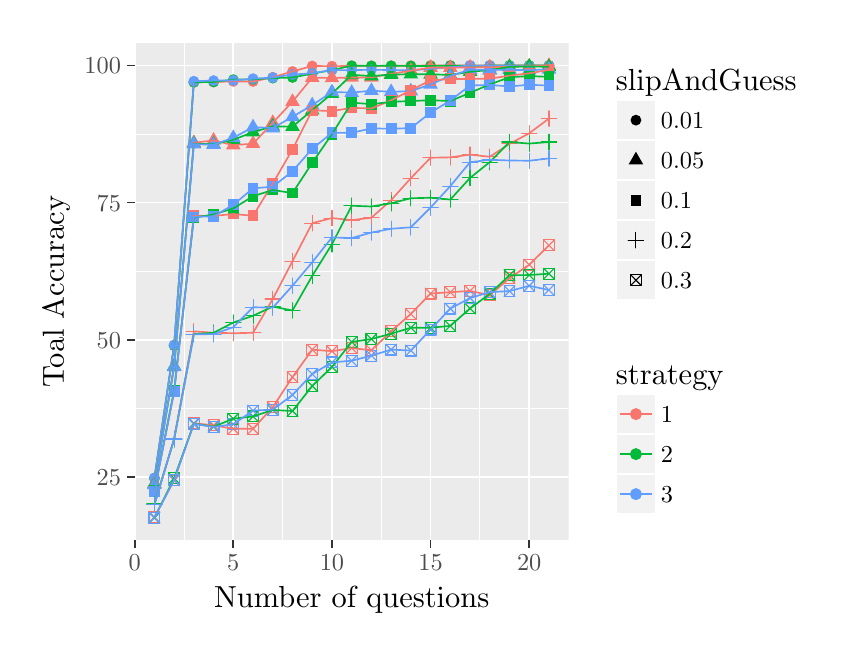
\begin{tikzpicture}[x=1pt,y=1pt]
\definecolor{fillColor}{RGB}{255,255,255}
\path[use as bounding box,fill=fillColor,fill opacity=0.00] (0,0) rectangle (289.08,216.81);
\begin{scope}
\path[clip] (  0.00,  0.00) rectangle (289.08,216.81);
\definecolor{drawColor}{RGB}{255,255,255}
\definecolor{fillColor}{RGB}{255,255,255}

\path[draw=drawColor,line width= 0.6pt,line join=round,line cap=round,fill=fillColor] (  0.00,  0.00) rectangle (289.08,216.81);
\end{scope}
\begin{scope}
\path[clip] ( 38.67, 31.53) rectangle (195.49,211.31);
\definecolor{fillColor}{gray}{0.92}

\path[fill=fillColor] ( 38.67, 31.53) rectangle (195.49,211.31);
\definecolor{drawColor}{RGB}{255,255,255}

\path[draw=drawColor,line width= 0.3pt,line join=round] ( 38.67, 79.28) --
	(195.49, 79.28);

\path[draw=drawColor,line width= 0.3pt,line join=round] ( 38.67,128.82) --
	(195.49,128.82);

\path[draw=drawColor,line width= 0.3pt,line join=round] ( 38.67,178.37) --
	(195.49,178.37);

\path[draw=drawColor,line width= 0.3pt,line join=round] ( 56.49, 31.53) --
	( 56.49,211.31);

\path[draw=drawColor,line width= 0.3pt,line join=round] ( 92.13, 31.53) --
	( 92.13,211.31);

\path[draw=drawColor,line width= 0.3pt,line join=round] (127.77, 31.53) --
	(127.77,211.31);

\path[draw=drawColor,line width= 0.3pt,line join=round] (163.41, 31.53) --
	(163.41,211.31);

\path[draw=drawColor,line width= 0.6pt,line join=round] ( 38.67, 54.51) --
	(195.49, 54.51);

\path[draw=drawColor,line width= 0.6pt,line join=round] ( 38.67,104.05) --
	(195.49,104.05);

\path[draw=drawColor,line width= 0.6pt,line join=round] ( 38.67,153.59) --
	(195.49,153.59);

\path[draw=drawColor,line width= 0.6pt,line join=round] ( 38.67,203.14) --
	(195.49,203.14);

\path[draw=drawColor,line width= 0.6pt,line join=round] ( 38.67, 31.53) --
	( 38.67,211.31);

\path[draw=drawColor,line width= 0.6pt,line join=round] ( 74.31, 31.53) --
	( 74.31,211.31);

\path[draw=drawColor,line width= 0.6pt,line join=round] (109.95, 31.53) --
	(109.95,211.31);

\path[draw=drawColor,line width= 0.6pt,line join=round] (145.59, 31.53) --
	(145.59,211.31);

\path[draw=drawColor,line width= 0.6pt,line join=round] (181.23, 31.53) --
	(181.23,211.31);
\definecolor{fillColor}{RGB}{248,118,109}

\path[fill=fillColor] ( 45.80, 54.08) circle (  1.96);

\path[fill=fillColor] ( 52.92,101.94) circle (  1.96);

\path[fill=fillColor] ( 60.05,197.07) circle (  1.96);

\path[fill=fillColor] ( 67.18,197.17) circle (  1.96);

\path[fill=fillColor] ( 74.31,197.40) circle (  1.96);

\path[fill=fillColor] ( 81.44,197.34) circle (  1.96);

\path[fill=fillColor] ( 88.57,198.90) circle (  1.96);

\path[fill=fillColor] ( 95.69,200.99) circle (  1.96);

\path[fill=fillColor] (102.82,202.98) circle (  1.96);

\path[fill=fillColor] (109.95,202.88) circle (  1.96);

\path[fill=fillColor] (117.08,202.99) circle (  1.96);

\path[fill=fillColor] (124.21,202.99) circle (  1.96);

\path[fill=fillColor] (131.34,203.02) circle (  1.96);

\path[fill=fillColor] (138.46,203.07) circle (  1.96);

\path[fill=fillColor] (145.59,203.14) circle (  1.96);

\path[fill=fillColor] (152.72,203.13) circle (  1.96);

\path[fill=fillColor] (159.85,203.13) circle (  1.96);

\path[fill=fillColor] (166.98,203.13) circle (  1.96);

\path[fill=fillColor] (174.11,203.11) circle (  1.96);

\path[fill=fillColor] (181.23,203.14) circle (  1.96);

\path[fill=fillColor] (188.36,203.14) circle (  1.96);
\definecolor{fillColor}{RGB}{0,186,56}

\path[fill=fillColor] ( 45.80, 53.96) circle (  1.96);

\path[fill=fillColor] ( 52.92,101.93) circle (  1.96);

\path[fill=fillColor] ( 60.05,197.06) circle (  1.96);

\path[fill=fillColor] ( 67.18,197.20) circle (  1.96);

\path[fill=fillColor] ( 74.31,198.04) circle (  1.96);

\path[fill=fillColor] ( 81.44,198.16) circle (  1.96);

\path[fill=fillColor] ( 88.57,198.57) circle (  1.96);

\path[fill=fillColor] ( 95.69,198.81) circle (  1.96);

\path[fill=fillColor] (102.82,200.21) circle (  1.96);

\path[fill=fillColor] (109.95,201.48) circle (  1.96);

\path[fill=fillColor] (117.08,203.05) circle (  1.96);

\path[fill=fillColor] (124.21,203.00) circle (  1.96);

\path[fill=fillColor] (131.34,203.04) circle (  1.96);

\path[fill=fillColor] (138.46,202.97) circle (  1.96);

\path[fill=fillColor] (145.59,202.99) circle (  1.96);

\path[fill=fillColor] (152.72,203.07) circle (  1.96);

\path[fill=fillColor] (159.85,203.03) circle (  1.96);

\path[fill=fillColor] (166.98,203.11) circle (  1.96);

\path[fill=fillColor] (174.11,203.13) circle (  1.96);

\path[fill=fillColor] (181.23,203.14) circle (  1.96);

\path[fill=fillColor] (188.36,203.14) circle (  1.96);
\definecolor{fillColor}{RGB}{97,156,255}

\path[fill=fillColor] ( 45.80, 54.10) circle (  1.96);

\path[fill=fillColor] ( 52.92,102.19) circle (  1.96);

\path[fill=fillColor] ( 60.05,197.46) circle (  1.96);

\path[fill=fillColor] ( 67.18,197.68) circle (  1.96);

\path[fill=fillColor] ( 74.31,197.73) circle (  1.96);

\path[fill=fillColor] ( 81.44,198.38) circle (  1.96);

\path[fill=fillColor] ( 88.57,198.77) circle (  1.96);

\path[fill=fillColor] ( 95.69,199.88) circle (  1.96);

\path[fill=fillColor] (102.82,200.31) circle (  1.96);

\path[fill=fillColor] (109.95,201.50) circle (  1.96);

\path[fill=fillColor] (117.08,201.45) circle (  1.96);

\path[fill=fillColor] (124.21,201.61) circle (  1.96);

\path[fill=fillColor] (131.34,201.49) circle (  1.96);

\path[fill=fillColor] (138.46,201.39) circle (  1.96);

\path[fill=fillColor] (145.59,201.94) circle (  1.96);

\path[fill=fillColor] (152.72,202.51) circle (  1.96);

\path[fill=fillColor] (159.85,203.11) circle (  1.96);

\path[fill=fillColor] (166.98,203.10) circle (  1.96);

\path[fill=fillColor] (174.11,203.08) circle (  1.96);

\path[fill=fillColor] (181.23,203.11) circle (  1.96);

\path[fill=fillColor] (188.36,203.10) circle (  1.96);
\definecolor{fillColor}{RGB}{248,118,109}

\path[fill=fillColor] ( 45.80, 55.21) --
	( 48.44, 50.63) --
	( 43.15, 50.63) --
	cycle;

\path[fill=fillColor] ( 52.92, 97.37) --
	( 55.57, 92.79) --
	( 50.28, 92.79) --
	cycle;

\path[fill=fillColor] ( 60.05,178.27) --
	( 62.69,173.69) --
	( 57.41,173.69) --
	cycle;

\path[fill=fillColor] ( 67.18,179.11) --
	( 69.82,174.53) --
	( 64.54,174.53) --
	cycle;

\path[fill=fillColor] ( 74.31,177.44) --
	( 76.95,172.87) --
	( 71.67,172.87) --
	cycle;

\path[fill=fillColor] ( 81.44,177.92) --
	( 84.08,173.34) --
	( 78.79,173.34) --
	cycle;

\path[fill=fillColor] ( 88.57,185.50) --
	( 91.21,180.92) --
	( 85.92,180.92) --
	cycle;

\path[fill=fillColor] ( 95.69,193.11) --
	( 98.34,188.53) --
	( 93.05,188.53) --
	cycle;

\path[fill=fillColor] (102.82,201.81) --
	(105.46,197.23) --
	(100.18,197.23) --
	cycle;

\path[fill=fillColor] (109.95,201.67) --
	(112.59,197.09) --
	(107.31,197.09) --
	cycle;

\path[fill=fillColor] (117.08,201.86) --
	(119.72,197.28) --
	(114.44,197.28) --
	cycle;

\path[fill=fillColor] (124.21,201.89) --
	(126.85,197.31) --
	(121.56,197.31) --
	cycle;

\path[fill=fillColor] (131.34,203.18) --
	(133.98,198.60) --
	(128.69,198.60) --
	cycle;

\path[fill=fillColor] (138.46,204.31) --
	(141.11,199.73) --
	(135.82,199.73) --
	cycle;

\path[fill=fillColor] (145.59,205.42) --
	(148.23,200.84) --
	(142.95,200.84) --
	cycle;

\path[fill=fillColor] (152.72,205.38) --
	(155.36,200.80) --
	(150.08,200.80) --
	cycle;

\path[fill=fillColor] (159.85,205.51) --
	(162.49,200.93) --
	(157.21,200.93) --
	cycle;

\path[fill=fillColor] (166.98,205.57) --
	(169.62,200.99) --
	(164.33,200.99) --
	cycle;

\path[fill=fillColor] (174.11,205.73) --
	(176.75,201.16) --
	(171.46,201.16) --
	cycle;

\path[fill=fillColor] (181.23,205.92) --
	(183.88,201.35) --
	(178.59,201.35) --
	cycle;

\path[fill=fillColor] (188.36,206.12) --
	(191.00,201.54) --
	(185.72,201.54) --
	cycle;
\definecolor{fillColor}{RGB}{0,186,56}

\path[fill=fillColor] ( 45.80, 54.89) --
	( 48.44, 50.32) --
	( 43.15, 50.32) --
	cycle;

\path[fill=fillColor] ( 52.92, 97.50) --
	( 55.57, 92.92) --
	( 50.28, 92.92) --
	cycle;

\path[fill=fillColor] ( 60.05,177.92) --
	( 62.69,173.34) --
	( 57.41,173.34) --
	cycle;

\path[fill=fillColor] ( 67.18,177.75) --
	( 69.82,173.17) --
	( 64.54,173.17) --
	cycle;

\path[fill=fillColor] ( 74.31,179.35) --
	( 76.95,174.77) --
	( 71.67,174.77) --
	cycle;

\path[fill=fillColor] ( 81.44,182.14) --
	( 84.08,177.56) --
	( 78.79,177.56) --
	cycle;

\path[fill=fillColor] ( 88.57,184.21) --
	( 91.21,179.63) --
	( 85.92,179.63) --
	cycle;

\path[fill=fillColor] ( 95.69,184.06) --
	( 98.34,179.49) --
	( 93.05,179.49) --
	cycle;

\path[fill=fillColor] (102.82,190.06) --
	(105.46,185.48) --
	(100.18,185.48) --
	cycle;

\path[fill=fillColor] (109.95,196.02) --
	(112.59,191.45) --
	(107.31,191.45) --
	cycle;

\path[fill=fillColor] (117.08,202.83) --
	(119.72,198.25) --
	(114.44,198.25) --
	cycle;

\path[fill=fillColor] (124.21,202.37) --
	(126.85,197.80) --
	(121.56,197.80) --
	cycle;

\path[fill=fillColor] (131.34,202.90) --
	(133.98,198.32) --
	(128.69,198.32) --
	cycle;

\path[fill=fillColor] (138.46,203.04) --
	(141.11,198.46) --
	(135.82,198.46) --
	cycle;

\path[fill=fillColor] (145.59,203.02) --
	(148.23,198.44) --
	(142.95,198.44) --
	cycle;

\path[fill=fillColor] (152.72,202.77) --
	(155.36,198.19) --
	(150.08,198.19) --
	cycle;

\path[fill=fillColor] (159.85,203.94) --
	(162.49,199.36) --
	(157.21,199.36) --
	cycle;

\path[fill=fillColor] (166.98,204.53) --
	(169.62,199.96) --
	(164.33,199.96) --
	cycle;

\path[fill=fillColor] (174.11,205.70) --
	(176.75,201.13) --
	(171.46,201.13) --
	cycle;

\path[fill=fillColor] (181.23,205.84) --
	(183.88,201.27) --
	(178.59,201.27) --
	cycle;

\path[fill=fillColor] (188.36,205.71) --
	(191.00,201.14) --
	(185.72,201.14) --
	cycle;
\definecolor{fillColor}{RGB}{97,156,255}

\path[fill=fillColor] ( 45.80, 54.62) --
	( 48.44, 50.05) --
	( 43.15, 50.05) --
	cycle;

\path[fill=fillColor] ( 52.92, 97.27) --
	( 55.57, 92.70) --
	( 50.28, 92.70) --
	cycle;

\path[fill=fillColor] ( 60.05,177.76) --
	( 62.69,173.18) --
	( 57.41,173.18) --
	cycle;

\path[fill=fillColor] ( 67.18,177.56) --
	( 69.82,172.99) --
	( 64.54,172.99) --
	cycle;

\path[fill=fillColor] ( 74.31,180.09) --
	( 76.95,175.51) --
	( 71.67,175.51) --
	cycle;

\path[fill=fillColor] ( 81.44,183.91) --
	( 84.08,179.34) --
	( 78.79,179.34) --
	cycle;

\path[fill=fillColor] ( 88.57,183.59) --
	( 91.21,179.01) --
	( 85.92,179.01) --
	cycle;

\path[fill=fillColor] ( 95.69,187.65) --
	( 98.34,183.07) --
	( 93.05,183.07) --
	cycle;

\path[fill=fillColor] (102.82,191.87) --
	(105.46,187.29) --
	(100.18,187.29) --
	cycle;

\path[fill=fillColor] (109.95,196.62) --
	(112.59,192.04) --
	(107.31,192.04) --
	cycle;

\path[fill=fillColor] (117.08,196.39) --
	(119.72,191.81) --
	(114.44,191.81) --
	cycle;

\path[fill=fillColor] (124.21,197.08) --
	(126.85,192.51) --
	(121.56,192.51) --
	cycle;

\path[fill=fillColor] (131.34,196.67) --
	(133.98,192.09) --
	(128.69,192.09) --
	cycle;

\path[fill=fillColor] (138.46,196.94) --
	(141.11,192.37) --
	(135.82,192.37) --
	cycle;

\path[fill=fillColor] (145.59,199.37) --
	(148.23,194.80) --
	(142.95,194.80) --
	cycle;

\path[fill=fillColor] (152.72,202.40) --
	(155.36,197.83) --
	(150.08,197.83) --
	cycle;

\path[fill=fillColor] (159.85,204.70) --
	(162.49,200.13) --
	(157.21,200.13) --
	cycle;

\path[fill=fillColor] (166.98,204.57) --
	(169.62,200.00) --
	(164.33,200.00) --
	cycle;

\path[fill=fillColor] (174.11,204.64) --
	(176.75,200.07) --
	(171.46,200.07) --
	cycle;

\path[fill=fillColor] (181.23,204.50) --
	(183.88,199.92) --
	(178.59,199.92) --
	cycle;

\path[fill=fillColor] (188.36,204.80) --
	(191.00,200.23) --
	(185.72,200.23) --
	cycle;
\definecolor{fillColor}{RGB}{248,118,109}

\path[fill=fillColor] ( 43.83, 47.26) --
	( 47.76, 47.26) --
	( 47.76, 51.19) --
	( 43.83, 51.19) --
	cycle;

\path[fill=fillColor] ( 50.96, 83.37) --
	( 54.89, 83.37) --
	( 54.89, 87.29) --
	( 50.96, 87.29) --
	cycle;

\path[fill=fillColor] ( 58.09,146.89) --
	( 62.01,146.89) --
	( 62.01,150.81) --
	( 58.09,150.81) --
	cycle;

\path[fill=fillColor] ( 65.22,146.81) --
	( 69.14,146.81) --
	( 69.14,150.73) --
	( 65.22,150.73) --
	cycle;

\path[fill=fillColor] ( 72.35,147.52) --
	( 76.27,147.52) --
	( 76.27,151.44) --
	( 72.35,151.44) --
	cycle;

\path[fill=fillColor] ( 79.47,146.89) --
	( 83.40,146.89) --
	( 83.40,150.81) --
	( 79.47,150.81) --
	cycle;

\path[fill=fillColor] ( 86.60,158.56) --
	( 90.53,158.56) --
	( 90.53,162.48) --
	( 86.60,162.48) --
	cycle;

\path[fill=fillColor] ( 93.73,170.86) --
	( 97.66,170.86) --
	( 97.66,174.78) --
	( 93.73,174.78) --
	cycle;

\path[fill=fillColor] (100.86,184.99) --
	(104.78,184.99) --
	(104.78,188.91) --
	(100.86,188.91) --
	cycle;

\path[fill=fillColor] (107.99,184.69) --
	(111.91,184.69) --
	(111.91,188.61) --
	(107.99,188.61) --
	cycle;

\path[fill=fillColor] (115.12,185.88) --
	(119.04,185.88) --
	(119.04,189.80) --
	(115.12,189.80) --
	cycle;

\path[fill=fillColor] (122.24,185.65) --
	(126.17,185.65) --
	(126.17,189.57) --
	(122.24,189.57) --
	cycle;

\path[fill=fillColor] (129.37,188.61) --
	(133.30,188.61) --
	(133.30,192.54) --
	(129.37,192.54) --
	cycle;

\path[fill=fillColor] (136.50,192.25) --
	(140.43,192.25) --
	(140.43,196.17) --
	(136.50,196.17) --
	cycle;

\path[fill=fillColor] (143.63,195.80) --
	(147.55,195.80) --
	(147.55,199.72) --
	(143.63,199.72) --
	cycle;

\path[fill=fillColor] (150.76,196.33) --
	(154.68,196.33) --
	(154.68,200.25) --
	(150.76,200.25) --
	cycle;

\path[fill=fillColor] (157.89,196.32) --
	(161.81,196.32) --
	(161.81,200.25) --
	(157.89,200.25) --
	cycle;

\path[fill=fillColor] (165.01,196.42) --
	(168.94,196.42) --
	(168.94,200.34) --
	(165.01,200.34) --
	cycle;

\path[fill=fillColor] (172.14,197.51) --
	(176.07,197.51) --
	(176.07,201.43) --
	(172.14,201.43) --
	cycle;

\path[fill=fillColor] (179.27,198.36) --
	(183.20,198.36) --
	(183.20,202.29) --
	(179.27,202.29) --
	cycle;

\path[fill=fillColor] (186.40,199.59) --
	(190.32,199.59) --
	(190.32,203.51) --
	(186.40,203.51) --
	cycle;
\definecolor{fillColor}{RGB}{0,186,56}

\path[fill=fillColor] ( 43.83, 47.68) --
	( 47.76, 47.68) --
	( 47.76, 51.60) --
	( 43.83, 51.60) --
	cycle;

\path[fill=fillColor] ( 50.96, 83.77) --
	( 54.89, 83.77) --
	( 54.89, 87.69) --
	( 50.96, 87.69) --
	cycle;

\path[fill=fillColor] ( 58.09,146.21) --
	( 62.01,146.21) --
	( 62.01,150.14) --
	( 58.09,150.14) --
	cycle;

\path[fill=fillColor] ( 65.22,147.34) --
	( 69.14,147.34) --
	( 69.14,151.27) --
	( 65.22,151.27) --
	cycle;

\path[fill=fillColor] ( 72.35,149.54) --
	( 76.27,149.54) --
	( 76.27,153.47) --
	( 72.35,153.47) --
	cycle;

\path[fill=fillColor] ( 79.47,153.96) --
	( 83.40,153.96) --
	( 83.40,157.88) --
	( 79.47,157.88) --
	cycle;

\path[fill=fillColor] ( 86.60,156.20) --
	( 90.53,156.20) --
	( 90.53,160.12) --
	( 86.60,160.12) --
	cycle;

\path[fill=fillColor] ( 93.73,155.08) --
	( 97.66,155.08) --
	( 97.66,159.00) --
	( 93.73,159.00) --
	cycle;

\path[fill=fillColor] (100.86,166.00) --
	(104.78,166.00) --
	(104.78,169.92) --
	(100.86,169.92) --
	cycle;

\path[fill=fillColor] (107.99,176.36) --
	(111.91,176.36) --
	(111.91,180.29) --
	(107.99,180.29) --
	cycle;

\path[fill=fillColor] (115.12,187.76) --
	(119.04,187.76) --
	(119.04,191.68) --
	(115.12,191.68) --
	cycle;

\path[fill=fillColor] (122.24,187.20) --
	(126.17,187.20) --
	(126.17,191.13) --
	(122.24,191.13) --
	cycle;

\path[fill=fillColor] (129.37,188.03) --
	(133.30,188.03) --
	(133.30,191.95) --
	(129.37,191.95) --
	cycle;

\path[fill=fillColor] (136.50,188.34) --
	(140.43,188.34) --
	(140.43,192.27) --
	(136.50,192.27) --
	cycle;

\path[fill=fillColor] (143.63,188.63) --
	(147.55,188.63) --
	(147.55,192.56) --
	(143.63,192.56) --
	cycle;

\path[fill=fillColor] (150.76,188.32) --
	(154.68,188.32) --
	(154.68,192.25) --
	(150.76,192.25) --
	cycle;

\path[fill=fillColor] (157.89,191.32) --
	(161.81,191.32) --
	(161.81,195.24) --
	(157.89,195.24) --
	cycle;

\path[fill=fillColor] (165.01,194.35) --
	(168.94,194.35) --
	(168.94,198.27) --
	(165.01,198.27) --
	cycle;

\path[fill=fillColor] (172.14,196.93) --
	(176.07,196.93) --
	(176.07,200.85) --
	(172.14,200.85) --
	cycle;

\path[fill=fillColor] (179.27,197.37) --
	(183.20,197.37) --
	(183.20,201.30) --
	(179.27,201.30) --
	cycle;

\path[fill=fillColor] (186.40,197.06) --
	(190.32,197.06) --
	(190.32,200.99) --
	(186.40,200.99) --
	cycle;
\definecolor{fillColor}{RGB}{97,156,255}

\path[fill=fillColor] ( 43.83, 47.32) --
	( 47.76, 47.32) --
	( 47.76, 51.25) --
	( 43.83, 51.25) --
	cycle;

\path[fill=fillColor] ( 50.96, 83.40) --
	( 54.89, 83.40) --
	( 54.89, 87.32) --
	( 50.96, 87.32) --
	cycle;

\path[fill=fillColor] ( 58.09,146.46) --
	( 62.01,146.46) --
	( 62.01,150.38) --
	( 58.09,150.38) --
	cycle;

\path[fill=fillColor] ( 65.22,146.71) --
	( 69.14,146.71) --
	( 69.14,150.63) --
	( 65.22,150.63) --
	cycle;

\path[fill=fillColor] ( 72.35,150.85) --
	( 76.27,150.85) --
	( 76.27,154.77) --
	( 72.35,154.77) --
	cycle;

\path[fill=fillColor] ( 79.47,156.79) --
	( 83.40,156.79) --
	( 83.40,160.72) --
	( 79.47,160.72) --
	cycle;

\path[fill=fillColor] ( 86.60,157.37) --
	( 90.53,157.37) --
	( 90.53,161.29) --
	( 86.60,161.29) --
	cycle;

\path[fill=fillColor] ( 93.73,162.98) --
	( 97.66,162.98) --
	( 97.66,166.90) --
	( 93.73,166.90) --
	cycle;

\path[fill=fillColor] (100.86,171.06) --
	(104.78,171.06) --
	(104.78,174.99) --
	(100.86,174.99) --
	cycle;

\path[fill=fillColor] (107.99,176.82) --
	(111.91,176.82) --
	(111.91,180.74) --
	(107.99,180.74) --
	cycle;

\path[fill=fillColor] (115.12,176.86) --
	(119.04,176.86) --
	(119.04,180.78) --
	(115.12,180.78) --
	cycle;

\path[fill=fillColor] (122.24,178.44) --
	(126.17,178.44) --
	(126.17,182.36) --
	(122.24,182.36) --
	cycle;

\path[fill=fillColor] (129.37,178.33) --
	(133.30,178.33) --
	(133.30,182.25) --
	(129.37,182.25) --
	cycle;

\path[fill=fillColor] (136.50,178.55) --
	(140.43,178.55) --
	(140.43,182.48) --
	(136.50,182.48) --
	cycle;

\path[fill=fillColor] (143.63,184.18) --
	(147.55,184.18) --
	(147.55,188.11) --
	(143.63,188.11) --
	cycle;

\path[fill=fillColor] (150.76,188.51) --
	(154.68,188.51) --
	(154.68,192.44) --
	(150.76,192.44) --
	cycle;

\path[fill=fillColor] (157.89,193.95) --
	(161.81,193.95) --
	(161.81,197.88) --
	(157.89,197.88) --
	cycle;

\path[fill=fillColor] (165.01,194.16) --
	(168.94,194.16) --
	(168.94,198.08) --
	(165.01,198.08) --
	cycle;

\path[fill=fillColor] (172.14,193.60) --
	(176.07,193.60) --
	(176.07,197.52) --
	(172.14,197.52) --
	cycle;

\path[fill=fillColor] (179.27,194.24) --
	(183.20,194.24) --
	(183.20,198.16) --
	(179.27,198.16) --
	cycle;

\path[fill=fillColor] (186.40,193.89) --
	(190.32,193.89) --
	(190.32,197.82) --
	(186.40,197.82) --
	cycle;
\definecolor{drawColor}{RGB}{248,118,109}

\path[draw=drawColor,line width= 0.4pt,line join=round,line cap=round] ( 43.02, 44.62) -- ( 48.57, 44.62);

\path[draw=drawColor,line width= 0.4pt,line join=round,line cap=round] ( 45.80, 41.84) -- ( 45.80, 47.39);

\path[draw=drawColor,line width= 0.4pt,line join=round,line cap=round] ( 50.15, 68.31) -- ( 55.70, 68.31);

\path[draw=drawColor,line width= 0.4pt,line join=round,line cap=round] ( 52.92, 65.53) -- ( 52.92, 71.08);

\path[draw=drawColor,line width= 0.4pt,line join=round,line cap=round] ( 57.28,107.06) -- ( 62.83,107.06);

\path[draw=drawColor,line width= 0.4pt,line join=round,line cap=round] ( 60.05,104.29) -- ( 60.05,109.84);

\path[draw=drawColor,line width= 0.4pt,line join=round,line cap=round] ( 64.41,106.59) -- ( 69.96,106.59);

\path[draw=drawColor,line width= 0.4pt,line join=round,line cap=round] ( 67.18,103.81) -- ( 67.18,109.36);

\path[draw=drawColor,line width= 0.4pt,line join=round,line cap=round] ( 71.53,106.39) -- ( 77.08,106.39);

\path[draw=drawColor,line width= 0.4pt,line join=round,line cap=round] ( 74.31,103.61) -- ( 74.31,109.16);

\path[draw=drawColor,line width= 0.4pt,line join=round,line cap=round] ( 78.66,106.56) -- ( 84.21,106.56);

\path[draw=drawColor,line width= 0.4pt,line join=round,line cap=round] ( 81.44,103.78) -- ( 81.44,109.33);

\path[draw=drawColor,line width= 0.4pt,line join=round,line cap=round] ( 85.79,118.75) -- ( 91.34,118.75);

\path[draw=drawColor,line width= 0.4pt,line join=round,line cap=round] ( 88.57,115.98) -- ( 88.57,121.53);

\path[draw=drawColor,line width= 0.4pt,line join=round,line cap=round] ( 92.92,132.43) -- ( 98.47,132.43);

\path[draw=drawColor,line width= 0.4pt,line join=round,line cap=round] ( 95.69,129.65) -- ( 95.69,135.20);

\path[draw=drawColor,line width= 0.4pt,line join=round,line cap=round] (100.05,146.17) -- (105.60,146.17);

\path[draw=drawColor,line width= 0.4pt,line join=round,line cap=round] (102.82,143.40) -- (102.82,148.95);

\path[draw=drawColor,line width= 0.4pt,line join=round,line cap=round] (107.18,148.01) -- (112.73,148.01);

\path[draw=drawColor,line width= 0.4pt,line join=round,line cap=round] (109.95,145.23) -- (109.95,150.78);

\path[draw=drawColor,line width= 0.4pt,line join=round,line cap=round] (114.30,147.26) -- (119.85,147.26);

\path[draw=drawColor,line width= 0.4pt,line join=round,line cap=round] (117.08,144.49) -- (117.08,150.04);

\path[draw=drawColor,line width= 0.4pt,line join=round,line cap=round] (121.43,148.14) -- (126.98,148.14);

\path[draw=drawColor,line width= 0.4pt,line join=round,line cap=round] (124.21,145.37) -- (124.21,150.92);

\path[draw=drawColor,line width= 0.4pt,line join=round,line cap=round] (128.56,154.49) -- (134.11,154.49);

\path[draw=drawColor,line width= 0.4pt,line join=round,line cap=round] (131.34,151.71) -- (131.34,157.26);

\path[draw=drawColor,line width= 0.4pt,line join=round,line cap=round] (135.69,162.43) -- (141.24,162.43);

\path[draw=drawColor,line width= 0.4pt,line join=round,line cap=round] (138.46,159.66) -- (138.46,165.21);

\path[draw=drawColor,line width= 0.4pt,line join=round,line cap=round] (142.82,169.81) -- (148.37,169.81);

\path[draw=drawColor,line width= 0.4pt,line join=round,line cap=round] (145.59,167.04) -- (145.59,172.59);

\path[draw=drawColor,line width= 0.4pt,line join=round,line cap=round] (149.95,169.94) -- (155.50,169.94);

\path[draw=drawColor,line width= 0.4pt,line join=round,line cap=round] (152.72,167.17) -- (152.72,172.72);

\path[draw=drawColor,line width= 0.4pt,line join=round,line cap=round] (157.07,170.93) -- (162.62,170.93);

\path[draw=drawColor,line width= 0.4pt,line join=round,line cap=round] (159.85,168.16) -- (159.85,173.71);

\path[draw=drawColor,line width= 0.4pt,line join=round,line cap=round] (164.20,170.16) -- (169.75,170.16);

\path[draw=drawColor,line width= 0.4pt,line join=round,line cap=round] (166.98,167.39) -- (166.98,172.94);

\path[draw=drawColor,line width= 0.4pt,line join=round,line cap=round] (171.33,174.82) -- (176.88,174.82);

\path[draw=drawColor,line width= 0.4pt,line join=round,line cap=round] (174.11,172.04) -- (174.11,177.59);

\path[draw=drawColor,line width= 0.4pt,line join=round,line cap=round] (178.46,178.65) -- (184.01,178.65);

\path[draw=drawColor,line width= 0.4pt,line join=round,line cap=round] (181.23,175.88) -- (181.23,181.43);

\path[draw=drawColor,line width= 0.4pt,line join=round,line cap=round] (185.59,183.96) -- (191.14,183.96);

\path[draw=drawColor,line width= 0.4pt,line join=round,line cap=round] (188.36,181.19) -- (188.36,186.74);
\definecolor{drawColor}{RGB}{0,186,56}

\path[draw=drawColor,line width= 0.4pt,line join=round,line cap=round] ( 43.02, 44.67) -- ( 48.57, 44.67);

\path[draw=drawColor,line width= 0.4pt,line join=round,line cap=round] ( 45.80, 41.89) -- ( 45.80, 47.44);

\path[draw=drawColor,line width= 0.4pt,line join=round,line cap=round] ( 50.15, 68.03) -- ( 55.70, 68.03);

\path[draw=drawColor,line width= 0.4pt,line join=round,line cap=round] ( 52.92, 65.26) -- ( 52.92, 70.81);

\path[draw=drawColor,line width= 0.4pt,line join=round,line cap=round] ( 57.28,106.07) -- ( 62.83,106.07);

\path[draw=drawColor,line width= 0.4pt,line join=round,line cap=round] ( 60.05,103.30) -- ( 60.05,108.85);

\path[draw=drawColor,line width= 0.4pt,line join=round,line cap=round] ( 64.41,106.56) -- ( 69.96,106.56);

\path[draw=drawColor,line width= 0.4pt,line join=round,line cap=round] ( 67.18,103.78) -- ( 67.18,109.33);

\path[draw=drawColor,line width= 0.4pt,line join=round,line cap=round] ( 71.53,110.26) -- ( 77.08,110.26);

\path[draw=drawColor,line width= 0.4pt,line join=round,line cap=round] ( 74.31,107.49) -- ( 74.31,113.04);

\path[draw=drawColor,line width= 0.4pt,line join=round,line cap=round] ( 78.66,112.72) -- ( 84.21,112.72);

\path[draw=drawColor,line width= 0.4pt,line join=round,line cap=round] ( 81.44,109.95) -- ( 81.44,115.50);

\path[draw=drawColor,line width= 0.4pt,line join=round,line cap=round] ( 85.79,116.01) -- ( 91.34,116.01);

\path[draw=drawColor,line width= 0.4pt,line join=round,line cap=round] ( 88.57,113.24) -- ( 88.57,118.79);

\path[draw=drawColor,line width= 0.4pt,line join=round,line cap=round] ( 92.92,114.62) -- ( 98.47,114.62);

\path[draw=drawColor,line width= 0.4pt,line join=round,line cap=round] ( 95.69,111.85) -- ( 95.69,117.40);

\path[draw=drawColor,line width= 0.4pt,line join=round,line cap=round] (100.05,127.12) -- (105.60,127.12);

\path[draw=drawColor,line width= 0.4pt,line join=round,line cap=round] (102.82,124.34) -- (102.82,129.89);

\path[draw=drawColor,line width= 0.4pt,line join=round,line cap=round] (107.18,138.56) -- (112.73,138.56);

\path[draw=drawColor,line width= 0.4pt,line join=round,line cap=round] (109.95,135.79) -- (109.95,141.34);

\path[draw=drawColor,line width= 0.4pt,line join=round,line cap=round] (114.30,152.47) -- (119.85,152.47);

\path[draw=drawColor,line width= 0.4pt,line join=round,line cap=round] (117.08,149.70) -- (117.08,155.25);

\path[draw=drawColor,line width= 0.4pt,line join=round,line cap=round] (121.43,152.19) -- (126.98,152.19);

\path[draw=drawColor,line width= 0.4pt,line join=round,line cap=round] (124.21,149.41) -- (124.21,154.96);

\path[draw=drawColor,line width= 0.4pt,line join=round,line cap=round] (128.56,153.35) -- (134.11,153.35);

\path[draw=drawColor,line width= 0.4pt,line join=round,line cap=round] (131.34,150.57) -- (131.34,156.12);

\path[draw=drawColor,line width= 0.4pt,line join=round,line cap=round] (135.69,155.17) -- (141.24,155.17);

\path[draw=drawColor,line width= 0.4pt,line join=round,line cap=round] (138.46,152.39) -- (138.46,157.94);

\path[draw=drawColor,line width= 0.4pt,line join=round,line cap=round] (142.82,155.35) -- (148.37,155.35);

\path[draw=drawColor,line width= 0.4pt,line join=round,line cap=round] (145.59,152.57) -- (145.59,158.12);

\path[draw=drawColor,line width= 0.4pt,line join=round,line cap=round] (149.95,154.70) -- (155.50,154.70);

\path[draw=drawColor,line width= 0.4pt,line join=round,line cap=round] (152.72,151.93) -- (152.72,157.48);

\path[draw=drawColor,line width= 0.4pt,line join=round,line cap=round] (157.07,162.51) -- (162.62,162.51);

\path[draw=drawColor,line width= 0.4pt,line join=round,line cap=round] (159.85,159.74) -- (159.85,165.29);

\path[draw=drawColor,line width= 0.4pt,line join=round,line cap=round] (164.20,168.24) -- (169.75,168.24);

\path[draw=drawColor,line width= 0.4pt,line join=round,line cap=round] (166.98,165.46) -- (166.98,171.01);

\path[draw=drawColor,line width= 0.4pt,line join=round,line cap=round] (171.33,175.48) -- (176.88,175.48);

\path[draw=drawColor,line width= 0.4pt,line join=round,line cap=round] (174.11,172.71) -- (174.11,178.26);

\path[draw=drawColor,line width= 0.4pt,line join=round,line cap=round] (178.46,174.93) -- (184.01,174.93);

\path[draw=drawColor,line width= 0.4pt,line join=round,line cap=round] (181.23,172.15) -- (181.23,177.70);

\path[draw=drawColor,line width= 0.4pt,line join=round,line cap=round] (185.59,175.48) -- (191.14,175.48);

\path[draw=drawColor,line width= 0.4pt,line join=round,line cap=round] (188.36,172.71) -- (188.36,178.26);
\definecolor{drawColor}{RGB}{97,156,255}

\path[draw=drawColor,line width= 0.4pt,line join=round,line cap=round] ( 43.02, 44.39) -- ( 48.57, 44.39);

\path[draw=drawColor,line width= 0.4pt,line join=round,line cap=round] ( 45.80, 41.61) -- ( 45.80, 47.16);

\path[draw=drawColor,line width= 0.4pt,line join=round,line cap=round] ( 50.15, 68.16) -- ( 55.70, 68.16);

\path[draw=drawColor,line width= 0.4pt,line join=round,line cap=round] ( 52.92, 65.39) -- ( 52.92, 70.94);

\path[draw=drawColor,line width= 0.4pt,line join=round,line cap=round] ( 57.28,105.98) -- ( 62.83,105.98);

\path[draw=drawColor,line width= 0.4pt,line join=round,line cap=round] ( 60.05,103.21) -- ( 60.05,108.76);

\path[draw=drawColor,line width= 0.4pt,line join=round,line cap=round] ( 64.41,106.09) -- ( 69.96,106.09);

\path[draw=drawColor,line width= 0.4pt,line join=round,line cap=round] ( 67.18,103.32) -- ( 67.18,108.87);

\path[draw=drawColor,line width= 0.4pt,line join=round,line cap=round] ( 71.53,108.58) -- ( 77.08,108.58);

\path[draw=drawColor,line width= 0.4pt,line join=round,line cap=round] ( 74.31,105.80) -- ( 74.31,111.35);

\path[draw=drawColor,line width= 0.4pt,line join=round,line cap=round] ( 78.66,115.79) -- ( 84.21,115.79);

\path[draw=drawColor,line width= 0.4pt,line join=round,line cap=round] ( 81.44,113.02) -- ( 81.44,118.57);

\path[draw=drawColor,line width= 0.4pt,line join=round,line cap=round] ( 85.79,115.63) -- ( 91.34,115.63);

\path[draw=drawColor,line width= 0.4pt,line join=round,line cap=round] ( 88.57,112.86) -- ( 88.57,118.41);

\path[draw=drawColor,line width= 0.4pt,line join=round,line cap=round] ( 92.92,123.56) -- ( 98.47,123.56);

\path[draw=drawColor,line width= 0.4pt,line join=round,line cap=round] ( 95.69,120.79) -- ( 95.69,126.34);

\path[draw=drawColor,line width= 0.4pt,line join=round,line cap=round] (100.05,132.05) -- (105.60,132.05);

\path[draw=drawColor,line width= 0.4pt,line join=round,line cap=round] (102.82,129.28) -- (102.82,134.83);

\path[draw=drawColor,line width= 0.4pt,line join=round,line cap=round] (107.18,141.01) -- (112.73,141.01);

\path[draw=drawColor,line width= 0.4pt,line join=round,line cap=round] (109.95,138.24) -- (109.95,143.78);

\path[draw=drawColor,line width= 0.4pt,line join=round,line cap=round] (114.30,140.79) -- (119.85,140.79);

\path[draw=drawColor,line width= 0.4pt,line join=round,line cap=round] (117.08,138.02) -- (117.08,143.57);

\path[draw=drawColor,line width= 0.4pt,line join=round,line cap=round] (121.43,142.78) -- (126.98,142.78);

\path[draw=drawColor,line width= 0.4pt,line join=round,line cap=round] (124.21,140.01) -- (124.21,145.56);

\path[draw=drawColor,line width= 0.4pt,line join=round,line cap=round] (128.56,144.14) -- (134.11,144.14);

\path[draw=drawColor,line width= 0.4pt,line join=round,line cap=round] (131.34,141.37) -- (131.34,146.92);

\path[draw=drawColor,line width= 0.4pt,line join=round,line cap=round] (135.69,144.67) -- (141.24,144.67);

\path[draw=drawColor,line width= 0.4pt,line join=round,line cap=round] (138.46,141.89) -- (138.46,147.44);

\path[draw=drawColor,line width= 0.4pt,line join=round,line cap=round] (142.82,151.80) -- (148.37,151.80);

\path[draw=drawColor,line width= 0.4pt,line join=round,line cap=round] (145.59,149.03) -- (145.59,154.58);

\path[draw=drawColor,line width= 0.4pt,line join=round,line cap=round] (149.95,159.56) -- (155.50,159.56);

\path[draw=drawColor,line width= 0.4pt,line join=round,line cap=round] (152.72,156.78) -- (152.72,162.33);

\path[draw=drawColor,line width= 0.4pt,line join=round,line cap=round] (157.07,168.20) -- (162.62,168.20);

\path[draw=drawColor,line width= 0.4pt,line join=round,line cap=round] (159.85,165.42) -- (159.85,170.97);

\path[draw=drawColor,line width= 0.4pt,line join=round,line cap=round] (164.20,169.04) -- (169.75,169.04);

\path[draw=drawColor,line width= 0.4pt,line join=round,line cap=round] (166.98,166.27) -- (166.98,171.82);

\path[draw=drawColor,line width= 0.4pt,line join=round,line cap=round] (171.33,168.82) -- (176.88,168.82);

\path[draw=drawColor,line width= 0.4pt,line join=round,line cap=round] (174.11,166.05) -- (174.11,171.60);

\path[draw=drawColor,line width= 0.4pt,line join=round,line cap=round] (178.46,168.72) -- (184.01,168.72);

\path[draw=drawColor,line width= 0.4pt,line join=round,line cap=round] (181.23,165.94) -- (181.23,171.49);

\path[draw=drawColor,line width= 0.4pt,line join=round,line cap=round] (185.59,169.56) -- (191.14,169.56);

\path[draw=drawColor,line width= 0.4pt,line join=round,line cap=round] (188.36,166.78) -- (188.36,172.33);
\definecolor{drawColor}{RGB}{248,118,109}

\path[draw=drawColor,line width= 0.4pt,line join=round,line cap=round] ( 43.83, 38.01) rectangle ( 47.76, 41.93);

\path[draw=drawColor,line width= 0.4pt,line join=round,line cap=round] ( 43.83, 38.01) -- ( 47.76, 41.93);

\path[draw=drawColor,line width= 0.4pt,line join=round,line cap=round] ( 43.83, 41.93) -- ( 47.76, 38.01);

\path[draw=drawColor,line width= 0.4pt,line join=round,line cap=round] ( 50.96, 51.25) rectangle ( 54.89, 55.17);

\path[draw=drawColor,line width= 0.4pt,line join=round,line cap=round] ( 50.96, 51.25) -- ( 54.89, 55.17);

\path[draw=drawColor,line width= 0.4pt,line join=round,line cap=round] ( 50.96, 55.17) -- ( 54.89, 51.25);

\path[draw=drawColor,line width= 0.4pt,line join=round,line cap=round] ( 58.09, 71.92) rectangle ( 62.01, 75.84);

\path[draw=drawColor,line width= 0.4pt,line join=round,line cap=round] ( 58.09, 71.92) -- ( 62.01, 75.84);

\path[draw=drawColor,line width= 0.4pt,line join=round,line cap=round] ( 58.09, 75.84) -- ( 62.01, 71.92);

\path[draw=drawColor,line width= 0.4pt,line join=round,line cap=round] ( 65.22, 71.18) rectangle ( 69.14, 75.11);

\path[draw=drawColor,line width= 0.4pt,line join=round,line cap=round] ( 65.22, 71.18) -- ( 69.14, 75.11);

\path[draw=drawColor,line width= 0.4pt,line join=round,line cap=round] ( 65.22, 75.11) -- ( 69.14, 71.18);

\path[draw=drawColor,line width= 0.4pt,line join=round,line cap=round] ( 72.35, 69.89) rectangle ( 76.27, 73.82);

\path[draw=drawColor,line width= 0.4pt,line join=round,line cap=round] ( 72.35, 69.89) -- ( 76.27, 73.82);

\path[draw=drawColor,line width= 0.4pt,line join=round,line cap=round] ( 72.35, 73.82) -- ( 76.27, 69.89);

\path[draw=drawColor,line width= 0.4pt,line join=round,line cap=round] ( 79.47, 69.91) rectangle ( 83.40, 73.84);

\path[draw=drawColor,line width= 0.4pt,line join=round,line cap=round] ( 79.47, 69.91) -- ( 83.40, 73.84);

\path[draw=drawColor,line width= 0.4pt,line join=round,line cap=round] ( 79.47, 73.84) -- ( 83.40, 69.91);

\path[draw=drawColor,line width= 0.4pt,line join=round,line cap=round] ( 86.60, 77.74) rectangle ( 90.53, 81.67);

\path[draw=drawColor,line width= 0.4pt,line join=round,line cap=round] ( 86.60, 77.74) -- ( 90.53, 81.67);

\path[draw=drawColor,line width= 0.4pt,line join=round,line cap=round] ( 86.60, 81.67) -- ( 90.53, 77.74);

\path[draw=drawColor,line width= 0.4pt,line join=round,line cap=round] ( 93.73, 88.57) rectangle ( 97.66, 92.50);

\path[draw=drawColor,line width= 0.4pt,line join=round,line cap=round] ( 93.73, 88.57) -- ( 97.66, 92.50);

\path[draw=drawColor,line width= 0.4pt,line join=round,line cap=round] ( 93.73, 92.50) -- ( 97.66, 88.57);

\path[draw=drawColor,line width= 0.4pt,line join=round,line cap=round] (100.86, 98.49) rectangle (104.78,102.42);

\path[draw=drawColor,line width= 0.4pt,line join=round,line cap=round] (100.86, 98.49) -- (104.78,102.42);

\path[draw=drawColor,line width= 0.4pt,line join=round,line cap=round] (100.86,102.42) -- (104.78, 98.49);

\path[draw=drawColor,line width= 0.4pt,line join=round,line cap=round] (107.99, 97.95) rectangle (111.91,101.87);

\path[draw=drawColor,line width= 0.4pt,line join=round,line cap=round] (107.99, 97.95) -- (111.91,101.87);

\path[draw=drawColor,line width= 0.4pt,line join=round,line cap=round] (107.99,101.87) -- (111.91, 97.95);

\path[draw=drawColor,line width= 0.4pt,line join=round,line cap=round] (115.12, 99.06) rectangle (119.04,102.98);

\path[draw=drawColor,line width= 0.4pt,line join=round,line cap=round] (115.12, 99.06) -- (119.04,102.98);

\path[draw=drawColor,line width= 0.4pt,line join=round,line cap=round] (115.12,102.98) -- (119.04, 99.06);

\path[draw=drawColor,line width= 0.4pt,line join=round,line cap=round] (122.24, 98.26) rectangle (126.17,102.19);

\path[draw=drawColor,line width= 0.4pt,line join=round,line cap=round] (122.24, 98.26) -- (126.17,102.19);

\path[draw=drawColor,line width= 0.4pt,line join=round,line cap=round] (122.24,102.19) -- (126.17, 98.26);

\path[draw=drawColor,line width= 0.4pt,line join=round,line cap=round] (129.37,105.12) rectangle (133.30,109.04);

\path[draw=drawColor,line width= 0.4pt,line join=round,line cap=round] (129.37,105.12) -- (133.30,109.04);

\path[draw=drawColor,line width= 0.4pt,line join=round,line cap=round] (129.37,109.04) -- (133.30,105.12);

\path[draw=drawColor,line width= 0.4pt,line join=round,line cap=round] (136.50,111.41) rectangle (140.43,115.34);

\path[draw=drawColor,line width= 0.4pt,line join=round,line cap=round] (136.50,111.41) -- (140.43,115.34);

\path[draw=drawColor,line width= 0.4pt,line join=round,line cap=round] (136.50,115.34) -- (140.43,111.41);

\path[draw=drawColor,line width= 0.4pt,line join=round,line cap=round] (143.63,118.76) rectangle (147.55,122.69);

\path[draw=drawColor,line width= 0.4pt,line join=round,line cap=round] (143.63,118.76) -- (147.55,122.69);

\path[draw=drawColor,line width= 0.4pt,line join=round,line cap=round] (143.63,122.69) -- (147.55,118.76);

\path[draw=drawColor,line width= 0.4pt,line join=round,line cap=round] (150.76,119.24) rectangle (154.68,123.16);

\path[draw=drawColor,line width= 0.4pt,line join=round,line cap=round] (150.76,119.24) -- (154.68,123.16);

\path[draw=drawColor,line width= 0.4pt,line join=round,line cap=round] (150.76,123.16) -- (154.68,119.24);

\path[draw=drawColor,line width= 0.4pt,line join=round,line cap=round] (157.89,119.74) rectangle (161.81,123.66);

\path[draw=drawColor,line width= 0.4pt,line join=round,line cap=round] (157.89,119.74) -- (161.81,123.66);

\path[draw=drawColor,line width= 0.4pt,line join=round,line cap=round] (157.89,123.66) -- (161.81,119.74);

\path[draw=drawColor,line width= 0.4pt,line join=round,line cap=round] (165.01,118.18) rectangle (168.94,122.10);

\path[draw=drawColor,line width= 0.4pt,line join=round,line cap=round] (165.01,118.18) -- (168.94,122.10);

\path[draw=drawColor,line width= 0.4pt,line join=round,line cap=round] (165.01,122.10) -- (168.94,118.18);

\path[draw=drawColor,line width= 0.4pt,line join=round,line cap=round] (172.14,124.33) rectangle (176.07,128.26);

\path[draw=drawColor,line width= 0.4pt,line join=round,line cap=round] (172.14,124.33) -- (176.07,128.26);

\path[draw=drawColor,line width= 0.4pt,line join=round,line cap=round] (172.14,128.26) -- (176.07,124.33);

\path[draw=drawColor,line width= 0.4pt,line join=round,line cap=round] (179.27,129.20) rectangle (183.20,133.12);

\path[draw=drawColor,line width= 0.4pt,line join=round,line cap=round] (179.27,129.20) -- (183.20,133.12);

\path[draw=drawColor,line width= 0.4pt,line join=round,line cap=round] (179.27,133.12) -- (183.20,129.20);

\path[draw=drawColor,line width= 0.4pt,line join=round,line cap=round] (186.40,136.19) rectangle (190.32,140.12);

\path[draw=drawColor,line width= 0.4pt,line join=round,line cap=round] (186.40,136.19) -- (190.32,140.12);

\path[draw=drawColor,line width= 0.4pt,line join=round,line cap=round] (186.40,140.12) -- (190.32,136.19);
\definecolor{drawColor}{RGB}{0,186,56}

\path[draw=drawColor,line width= 0.4pt,line join=round,line cap=round] ( 43.83, 37.74) rectangle ( 47.76, 41.66);

\path[draw=drawColor,line width= 0.4pt,line join=round,line cap=round] ( 43.83, 37.74) -- ( 47.76, 41.66);

\path[draw=drawColor,line width= 0.4pt,line join=round,line cap=round] ( 43.83, 41.66) -- ( 47.76, 37.74);

\path[draw=drawColor,line width= 0.4pt,line join=round,line cap=round] ( 50.96, 52.01) rectangle ( 54.89, 55.93);

\path[draw=drawColor,line width= 0.4pt,line join=round,line cap=round] ( 50.96, 52.01) -- ( 54.89, 55.93);

\path[draw=drawColor,line width= 0.4pt,line join=round,line cap=round] ( 50.96, 55.93) -- ( 54.89, 52.01);

\path[draw=drawColor,line width= 0.4pt,line join=round,line cap=round] ( 58.09, 71.76) rectangle ( 62.01, 75.68);

\path[draw=drawColor,line width= 0.4pt,line join=round,line cap=round] ( 58.09, 71.76) -- ( 62.01, 75.68);

\path[draw=drawColor,line width= 0.4pt,line join=round,line cap=round] ( 58.09, 75.68) -- ( 62.01, 71.76);

\path[draw=drawColor,line width= 0.4pt,line join=round,line cap=round] ( 65.22, 70.66) rectangle ( 69.14, 74.58);

\path[draw=drawColor,line width= 0.4pt,line join=round,line cap=round] ( 65.22, 70.66) -- ( 69.14, 74.58);

\path[draw=drawColor,line width= 0.4pt,line join=round,line cap=round] ( 65.22, 74.58) -- ( 69.14, 70.66);

\path[draw=drawColor,line width= 0.4pt,line join=round,line cap=round] ( 72.35, 73.56) rectangle ( 76.27, 77.48);

\path[draw=drawColor,line width= 0.4pt,line join=round,line cap=round] ( 72.35, 73.56) -- ( 76.27, 77.48);

\path[draw=drawColor,line width= 0.4pt,line join=round,line cap=round] ( 72.35, 77.48) -- ( 76.27, 73.56);

\path[draw=drawColor,line width= 0.4pt,line join=round,line cap=round] ( 79.47, 74.36) rectangle ( 83.40, 78.29);

\path[draw=drawColor,line width= 0.4pt,line join=round,line cap=round] ( 79.47, 74.36) -- ( 83.40, 78.29);

\path[draw=drawColor,line width= 0.4pt,line join=round,line cap=round] ( 79.47, 78.29) -- ( 83.40, 74.36);

\path[draw=drawColor,line width= 0.4pt,line join=round,line cap=round] ( 86.60, 76.72) rectangle ( 90.53, 80.65);

\path[draw=drawColor,line width= 0.4pt,line join=round,line cap=round] ( 86.60, 76.72) -- ( 90.53, 80.65);

\path[draw=drawColor,line width= 0.4pt,line join=round,line cap=round] ( 86.60, 80.65) -- ( 90.53, 76.72);

\path[draw=drawColor,line width= 0.4pt,line join=round,line cap=round] ( 93.73, 76.32) rectangle ( 97.66, 80.24);

\path[draw=drawColor,line width= 0.4pt,line join=round,line cap=round] ( 93.73, 76.32) -- ( 97.66, 80.24);

\path[draw=drawColor,line width= 0.4pt,line join=round,line cap=round] ( 93.73, 80.24) -- ( 97.66, 76.32);

\path[draw=drawColor,line width= 0.4pt,line join=round,line cap=round] (100.86, 85.37) rectangle (104.78, 89.30);

\path[draw=drawColor,line width= 0.4pt,line join=round,line cap=round] (100.86, 85.37) -- (104.78, 89.30);

\path[draw=drawColor,line width= 0.4pt,line join=round,line cap=round] (100.86, 89.30) -- (104.78, 85.37);

\path[draw=drawColor,line width= 0.4pt,line join=round,line cap=round] (107.99, 92.25) rectangle (111.91, 96.17);

\path[draw=drawColor,line width= 0.4pt,line join=round,line cap=round] (107.99, 92.25) -- (111.91, 96.17);

\path[draw=drawColor,line width= 0.4pt,line join=round,line cap=round] (107.99, 96.17) -- (111.91, 92.25);

\path[draw=drawColor,line width= 0.4pt,line join=round,line cap=round] (115.12,101.31) rectangle (119.04,105.23);

\path[draw=drawColor,line width= 0.4pt,line join=round,line cap=round] (115.12,101.31) -- (119.04,105.23);

\path[draw=drawColor,line width= 0.4pt,line join=round,line cap=round] (115.12,105.23) -- (119.04,101.31);

\path[draw=drawColor,line width= 0.4pt,line join=round,line cap=round] (122.24,102.33) rectangle (126.17,106.25);

\path[draw=drawColor,line width= 0.4pt,line join=round,line cap=round] (122.24,102.33) -- (126.17,106.25);

\path[draw=drawColor,line width= 0.4pt,line join=round,line cap=round] (122.24,106.25) -- (126.17,102.33);

\path[draw=drawColor,line width= 0.4pt,line join=round,line cap=round] (129.37,104.27) rectangle (133.30,108.19);

\path[draw=drawColor,line width= 0.4pt,line join=round,line cap=round] (129.37,104.27) -- (133.30,108.19);

\path[draw=drawColor,line width= 0.4pt,line join=round,line cap=round] (129.37,108.19) -- (133.30,104.27);

\path[draw=drawColor,line width= 0.4pt,line join=round,line cap=round] (136.50,106.42) rectangle (140.43,110.34);

\path[draw=drawColor,line width= 0.4pt,line join=round,line cap=round] (136.50,106.42) -- (140.43,110.34);

\path[draw=drawColor,line width= 0.4pt,line join=round,line cap=round] (136.50,110.34) -- (140.43,106.42);

\path[draw=drawColor,line width= 0.4pt,line join=round,line cap=round] (143.63,106.43) rectangle (147.55,110.35);

\path[draw=drawColor,line width= 0.4pt,line join=round,line cap=round] (143.63,106.43) -- (147.55,110.35);

\path[draw=drawColor,line width= 0.4pt,line join=round,line cap=round] (143.63,110.35) -- (147.55,106.43);

\path[draw=drawColor,line width= 0.4pt,line join=round,line cap=round] (150.76,107.09) rectangle (154.68,111.02);

\path[draw=drawColor,line width= 0.4pt,line join=round,line cap=round] (150.76,107.09) -- (154.68,111.02);

\path[draw=drawColor,line width= 0.4pt,line join=round,line cap=round] (150.76,111.02) -- (154.68,107.09);

\path[draw=drawColor,line width= 0.4pt,line join=round,line cap=round] (157.89,113.39) rectangle (161.81,117.32);

\path[draw=drawColor,line width= 0.4pt,line join=round,line cap=round] (157.89,113.39) -- (161.81,117.32);

\path[draw=drawColor,line width= 0.4pt,line join=round,line cap=round] (157.89,117.32) -- (161.81,113.39);

\path[draw=drawColor,line width= 0.4pt,line join=round,line cap=round] (165.01,118.65) rectangle (168.94,122.57);

\path[draw=drawColor,line width= 0.4pt,line join=round,line cap=round] (165.01,118.65) -- (168.94,122.57);

\path[draw=drawColor,line width= 0.4pt,line join=round,line cap=round] (165.01,122.57) -- (168.94,118.65);

\path[draw=drawColor,line width= 0.4pt,line join=round,line cap=round] (172.14,125.38) rectangle (176.07,129.31);

\path[draw=drawColor,line width= 0.4pt,line join=round,line cap=round] (172.14,125.38) -- (176.07,129.31);

\path[draw=drawColor,line width= 0.4pt,line join=round,line cap=round] (172.14,129.31) -- (176.07,125.38);

\path[draw=drawColor,line width= 0.4pt,line join=round,line cap=round] (179.27,125.45) rectangle (183.20,129.38);

\path[draw=drawColor,line width= 0.4pt,line join=round,line cap=round] (179.27,125.45) -- (183.20,129.38);

\path[draw=drawColor,line width= 0.4pt,line join=round,line cap=round] (179.27,129.38) -- (183.20,125.45);

\path[draw=drawColor,line width= 0.4pt,line join=round,line cap=round] (186.40,125.94) rectangle (190.32,129.86);

\path[draw=drawColor,line width= 0.4pt,line join=round,line cap=round] (186.40,125.94) -- (190.32,129.86);

\path[draw=drawColor,line width= 0.4pt,line join=round,line cap=round] (186.40,129.86) -- (190.32,125.94);
\definecolor{drawColor}{RGB}{97,156,255}

\path[draw=drawColor,line width= 0.4pt,line join=round,line cap=round] ( 43.83, 37.80) rectangle ( 47.76, 41.72);

\path[draw=drawColor,line width= 0.4pt,line join=round,line cap=round] ( 43.83, 37.80) -- ( 47.76, 41.72);

\path[draw=drawColor,line width= 0.4pt,line join=round,line cap=round] ( 43.83, 41.72) -- ( 47.76, 37.80);

\path[draw=drawColor,line width= 0.4pt,line join=round,line cap=round] ( 50.96, 51.46) rectangle ( 54.89, 55.39);

\path[draw=drawColor,line width= 0.4pt,line join=round,line cap=round] ( 50.96, 51.46) -- ( 54.89, 55.39);

\path[draw=drawColor,line width= 0.4pt,line join=round,line cap=round] ( 50.96, 55.39) -- ( 54.89, 51.46);

\path[draw=drawColor,line width= 0.4pt,line join=round,line cap=round] ( 58.09, 71.68) rectangle ( 62.01, 75.60);

\path[draw=drawColor,line width= 0.4pt,line join=round,line cap=round] ( 58.09, 71.68) -- ( 62.01, 75.60);

\path[draw=drawColor,line width= 0.4pt,line join=round,line cap=round] ( 58.09, 75.60) -- ( 62.01, 71.68);

\path[draw=drawColor,line width= 0.4pt,line join=round,line cap=round] ( 65.22, 70.56) rectangle ( 69.14, 74.48);

\path[draw=drawColor,line width= 0.4pt,line join=round,line cap=round] ( 65.22, 70.56) -- ( 69.14, 74.48);

\path[draw=drawColor,line width= 0.4pt,line join=round,line cap=round] ( 65.22, 74.48) -- ( 69.14, 70.56);

\path[draw=drawColor,line width= 0.4pt,line join=round,line cap=round] ( 72.35, 71.55) rectangle ( 76.27, 75.47);

\path[draw=drawColor,line width= 0.4pt,line join=round,line cap=round] ( 72.35, 71.55) -- ( 76.27, 75.47);

\path[draw=drawColor,line width= 0.4pt,line join=round,line cap=round] ( 72.35, 75.47) -- ( 76.27, 71.55);

\path[draw=drawColor,line width= 0.4pt,line join=round,line cap=round] ( 79.47, 76.48) rectangle ( 83.40, 80.41);

\path[draw=drawColor,line width= 0.4pt,line join=round,line cap=round] ( 79.47, 76.48) -- ( 83.40, 80.41);

\path[draw=drawColor,line width= 0.4pt,line join=round,line cap=round] ( 79.47, 80.41) -- ( 83.40, 76.48);

\path[draw=drawColor,line width= 0.4pt,line join=round,line cap=round] ( 86.60, 76.82) rectangle ( 90.53, 80.74);

\path[draw=drawColor,line width= 0.4pt,line join=round,line cap=round] ( 86.60, 76.82) -- ( 90.53, 80.74);

\path[draw=drawColor,line width= 0.4pt,line join=round,line cap=round] ( 86.60, 80.74) -- ( 90.53, 76.82);

\path[draw=drawColor,line width= 0.4pt,line join=round,line cap=round] ( 93.73, 82.14) rectangle ( 97.66, 86.07);

\path[draw=drawColor,line width= 0.4pt,line join=round,line cap=round] ( 93.73, 82.14) -- ( 97.66, 86.07);

\path[draw=drawColor,line width= 0.4pt,line join=round,line cap=round] ( 93.73, 86.07) -- ( 97.66, 82.14);

\path[draw=drawColor,line width= 0.4pt,line join=round,line cap=round] (100.86, 89.68) rectangle (104.78, 93.61);

\path[draw=drawColor,line width= 0.4pt,line join=round,line cap=round] (100.86, 89.68) -- (104.78, 93.61);

\path[draw=drawColor,line width= 0.4pt,line join=round,line cap=round] (100.86, 93.61) -- (104.78, 89.68);

\path[draw=drawColor,line width= 0.4pt,line join=round,line cap=round] (107.99, 93.89) rectangle (111.91, 97.82);

\path[draw=drawColor,line width= 0.4pt,line join=round,line cap=round] (107.99, 93.89) -- (111.91, 97.82);

\path[draw=drawColor,line width= 0.4pt,line join=round,line cap=round] (107.99, 97.82) -- (111.91, 93.89);

\path[draw=drawColor,line width= 0.4pt,line join=round,line cap=round] (115.12, 94.50) rectangle (119.04, 98.42);

\path[draw=drawColor,line width= 0.4pt,line join=round,line cap=round] (115.12, 94.50) -- (119.04, 98.42);

\path[draw=drawColor,line width= 0.4pt,line join=round,line cap=round] (115.12, 98.42) -- (119.04, 94.50);

\path[draw=drawColor,line width= 0.4pt,line join=round,line cap=round] (122.24, 96.34) rectangle (126.17,100.27);

\path[draw=drawColor,line width= 0.4pt,line join=round,line cap=round] (122.24, 96.34) -- (126.17,100.27);

\path[draw=drawColor,line width= 0.4pt,line join=round,line cap=round] (122.24,100.27) -- (126.17, 96.34);

\path[draw=drawColor,line width= 0.4pt,line join=round,line cap=round] (129.37, 98.51) rectangle (133.30,102.44);

\path[draw=drawColor,line width= 0.4pt,line join=round,line cap=round] (129.37, 98.51) -- (133.30,102.44);

\path[draw=drawColor,line width= 0.4pt,line join=round,line cap=round] (129.37,102.44) -- (133.30, 98.51);

\path[draw=drawColor,line width= 0.4pt,line join=round,line cap=round] (136.50, 98.18) rectangle (140.43,102.11);

\path[draw=drawColor,line width= 0.4pt,line join=round,line cap=round] (136.50, 98.18) -- (140.43,102.11);

\path[draw=drawColor,line width= 0.4pt,line join=round,line cap=round] (136.50,102.11) -- (140.43, 98.18);

\path[draw=drawColor,line width= 0.4pt,line join=round,line cap=round] (143.63,105.75) rectangle (147.55,109.68);

\path[draw=drawColor,line width= 0.4pt,line join=round,line cap=round] (143.63,105.75) -- (147.55,109.68);

\path[draw=drawColor,line width= 0.4pt,line join=round,line cap=round] (143.63,109.68) -- (147.55,105.75);

\path[draw=drawColor,line width= 0.4pt,line join=round,line cap=round] (150.76,113.35) rectangle (154.68,117.28);

\path[draw=drawColor,line width= 0.4pt,line join=round,line cap=round] (150.76,113.35) -- (154.68,117.28);

\path[draw=drawColor,line width= 0.4pt,line join=round,line cap=round] (150.76,117.28) -- (154.68,113.35);

\path[draw=drawColor,line width= 0.4pt,line join=round,line cap=round] (157.89,117.14) rectangle (161.81,121.06);

\path[draw=drawColor,line width= 0.4pt,line join=round,line cap=round] (157.89,117.14) -- (161.81,121.06);

\path[draw=drawColor,line width= 0.4pt,line join=round,line cap=round] (157.89,121.06) -- (161.81,117.14);

\path[draw=drawColor,line width= 0.4pt,line join=round,line cap=round] (165.01,119.31) rectangle (168.94,123.23);

\path[draw=drawColor,line width= 0.4pt,line join=round,line cap=round] (165.01,119.31) -- (168.94,123.23);

\path[draw=drawColor,line width= 0.4pt,line join=round,line cap=round] (165.01,123.23) -- (168.94,119.31);

\path[draw=drawColor,line width= 0.4pt,line join=round,line cap=round] (172.14,119.65) rectangle (176.07,123.57);

\path[draw=drawColor,line width= 0.4pt,line join=round,line cap=round] (172.14,119.65) -- (176.07,123.57);

\path[draw=drawColor,line width= 0.4pt,line join=round,line cap=round] (172.14,123.57) -- (176.07,119.65);

\path[draw=drawColor,line width= 0.4pt,line join=round,line cap=round] (179.27,121.58) rectangle (183.20,125.50);

\path[draw=drawColor,line width= 0.4pt,line join=round,line cap=round] (179.27,121.58) -- (183.20,125.50);

\path[draw=drawColor,line width= 0.4pt,line join=round,line cap=round] (179.27,125.50) -- (183.20,121.58);

\path[draw=drawColor,line width= 0.4pt,line join=round,line cap=round] (186.40,120.05) rectangle (190.32,123.98);

\path[draw=drawColor,line width= 0.4pt,line join=round,line cap=round] (186.40,120.05) -- (190.32,123.98);

\path[draw=drawColor,line width= 0.4pt,line join=round,line cap=round] (186.40,123.98) -- (190.32,120.05);
\definecolor{drawColor}{RGB}{248,118,109}

\path[draw=drawColor,line width= 0.6pt,line join=round] ( 45.80, 54.08) --
	( 52.92,101.94) --
	( 60.05,197.07) --
	( 67.18,197.17) --
	( 74.31,197.40) --
	( 81.44,197.34) --
	( 88.57,198.90) --
	( 95.69,200.99) --
	(102.82,202.98) --
	(109.95,202.88) --
	(117.08,202.99) --
	(124.21,202.99) --
	(131.34,203.02) --
	(138.46,203.07) --
	(145.59,203.14) --
	(152.72,203.13) --
	(159.85,203.13) --
	(166.98,203.13) --
	(174.11,203.11) --
	(181.23,203.14) --
	(188.36,203.14);
\definecolor{drawColor}{RGB}{0,186,56}

\path[draw=drawColor,line width= 0.6pt,line join=round] ( 45.80, 53.96) --
	( 52.92,101.93) --
	( 60.05,197.06) --
	( 67.18,197.20) --
	( 74.31,198.04) --
	( 81.44,198.16) --
	( 88.57,198.57) --
	( 95.69,198.81) --
	(102.82,200.21) --
	(109.95,201.48) --
	(117.08,203.05) --
	(124.21,203.00) --
	(131.34,203.04) --
	(138.46,202.97) --
	(145.59,202.99) --
	(152.72,203.07) --
	(159.85,203.03) --
	(166.98,203.11) --
	(174.11,203.13) --
	(181.23,203.14) --
	(188.36,203.14);
\definecolor{drawColor}{RGB}{97,156,255}

\path[draw=drawColor,line width= 0.6pt,line join=round] ( 45.80, 54.10) --
	( 52.92,102.19) --
	( 60.05,197.46) --
	( 67.18,197.68) --
	( 74.31,197.73) --
	( 81.44,198.38) --
	( 88.57,198.77) --
	( 95.69,199.88) --
	(102.82,200.31) --
	(109.95,201.50) --
	(117.08,201.45) --
	(124.21,201.61) --
	(131.34,201.49) --
	(138.46,201.39) --
	(145.59,201.94) --
	(152.72,202.51) --
	(159.85,203.11) --
	(166.98,203.10) --
	(174.11,203.08) --
	(181.23,203.11) --
	(188.36,203.10);
\definecolor{drawColor}{RGB}{248,118,109}

\path[draw=drawColor,line width= 0.6pt,line join=round] ( 45.80, 52.16) --
	( 52.92, 94.32) --
	( 60.05,175.22) --
	( 67.18,176.06) --
	( 74.31,174.39) --
	( 81.44,174.87) --
	( 88.57,182.45) --
	( 95.69,190.06) --
	(102.82,198.76) --
	(109.95,198.62) --
	(117.08,198.81) --
	(124.21,198.84) --
	(131.34,200.13) --
	(138.46,201.26) --
	(145.59,202.37) --
	(152.72,202.33) --
	(159.85,202.45) --
	(166.98,202.51) --
	(174.11,202.68) --
	(181.23,202.87) --
	(188.36,203.07);
\definecolor{drawColor}{RGB}{0,186,56}

\path[draw=drawColor,line width= 0.6pt,line join=round] ( 45.80, 51.84) --
	( 52.92, 94.45) --
	( 60.05,174.87) --
	( 67.18,174.70) --
	( 74.31,176.30) --
	( 81.44,179.09) --
	( 88.57,181.16) --
	( 95.69,181.01) --
	(102.82,187.01) --
	(109.95,192.97) --
	(117.08,199.78) --
	(124.21,199.32) --
	(131.34,199.85) --
	(138.46,199.99) --
	(145.59,199.97) --
	(152.72,199.72) --
	(159.85,200.89) --
	(166.98,201.48) --
	(174.11,202.65) --
	(181.23,202.79) --
	(188.36,202.66);
\definecolor{drawColor}{RGB}{97,156,255}

\path[draw=drawColor,line width= 0.6pt,line join=round] ( 45.80, 51.57) --
	( 52.92, 94.22) --
	( 60.05,174.71) --
	( 67.18,174.51) --
	( 74.31,177.04) --
	( 81.44,180.86) --
	( 88.57,180.54) --
	( 95.69,184.60) --
	(102.82,188.82) --
	(109.95,193.57) --
	(117.08,193.34) --
	(124.21,194.03) --
	(131.34,193.62) --
	(138.46,193.89) --
	(145.59,196.32) --
	(152.72,199.35) --
	(159.85,201.65) --
	(166.98,201.52) --
	(174.11,201.59) --
	(181.23,201.44) --
	(188.36,201.75);
\definecolor{drawColor}{RGB}{248,118,109}

\path[draw=drawColor,line width= 0.6pt,line join=round] ( 45.80, 49.22) --
	( 52.92, 85.33) --
	( 60.05,148.85) --
	( 67.18,148.77) --
	( 74.31,149.48) --
	( 81.44,148.85) --
	( 88.57,160.52) --
	( 95.69,172.82) --
	(102.82,186.95) --
	(109.95,186.65) --
	(117.08,187.84) --
	(124.21,187.61) --
	(131.34,190.57) --
	(138.46,194.21) --
	(145.59,197.76) --
	(152.72,198.29) --
	(159.85,198.28) --
	(166.98,198.38) --
	(174.11,199.47) --
	(181.23,200.32) --
	(188.36,201.55);
\definecolor{drawColor}{RGB}{0,186,56}

\path[draw=drawColor,line width= 0.6pt,line join=round] ( 45.80, 49.64) --
	( 52.92, 85.73) --
	( 60.05,148.17) --
	( 67.18,149.30) --
	( 74.31,151.50) --
	( 81.44,155.92) --
	( 88.57,158.16) --
	( 95.69,157.04) --
	(102.82,167.96) --
	(109.95,178.33) --
	(117.08,189.72) --
	(124.21,189.17) --
	(131.34,189.99) --
	(138.46,190.31) --
	(145.59,190.59) --
	(152.72,190.29) --
	(159.85,193.28) --
	(166.98,196.31) --
	(174.11,198.89) --
	(181.23,199.33) --
	(188.36,199.03);
\definecolor{drawColor}{RGB}{97,156,255}

\path[draw=drawColor,line width= 0.6pt,line join=round] ( 45.80, 49.28) --
	( 52.92, 85.36) --
	( 60.05,148.42) --
	( 67.18,148.67) --
	( 74.31,152.81) --
	( 81.44,158.76) --
	( 88.57,159.33) --
	( 95.69,164.94) --
	(102.82,173.03) --
	(109.95,178.78) --
	(117.08,178.82) --
	(124.21,180.40) --
	(131.34,180.29) --
	(138.46,180.52) --
	(145.59,186.14) --
	(152.72,190.47) --
	(159.85,195.91) --
	(166.98,196.12) --
	(174.11,195.56) --
	(181.23,196.20) --
	(188.36,195.86);
\definecolor{drawColor}{RGB}{248,118,109}

\path[draw=drawColor,line width= 0.6pt,line join=round] ( 45.80, 44.62) --
	( 52.92, 68.31) --
	( 60.05,107.06) --
	( 67.18,106.59) --
	( 74.31,106.39) --
	( 81.44,106.56) --
	( 88.57,118.75) --
	( 95.69,132.43) --
	(102.82,146.17) --
	(109.95,148.01) --
	(117.08,147.26) --
	(124.21,148.14) --
	(131.34,154.49) --
	(138.46,162.43) --
	(145.59,169.81) --
	(152.72,169.94) --
	(159.85,170.93) --
	(166.98,170.16) --
	(174.11,174.82) --
	(181.23,178.65) --
	(188.36,183.96);
\definecolor{drawColor}{RGB}{0,186,56}

\path[draw=drawColor,line width= 0.6pt,line join=round] ( 45.80, 44.67) --
	( 52.92, 68.03) --
	( 60.05,106.07) --
	( 67.18,106.56) --
	( 74.31,110.26) --
	( 81.44,112.72) --
	( 88.57,116.01) --
	( 95.69,114.62) --
	(102.82,127.12) --
	(109.95,138.56) --
	(117.08,152.47) --
	(124.21,152.19) --
	(131.34,153.35) --
	(138.46,155.17) --
	(145.59,155.35) --
	(152.72,154.70) --
	(159.85,162.51) --
	(166.98,168.24) --
	(174.11,175.48) --
	(181.23,174.93) --
	(188.36,175.48);
\definecolor{drawColor}{RGB}{97,156,255}

\path[draw=drawColor,line width= 0.6pt,line join=round] ( 45.80, 44.39) --
	( 52.92, 68.16) --
	( 60.05,105.98) --
	( 67.18,106.09) --
	( 74.31,108.58) --
	( 81.44,115.79) --
	( 88.57,115.63) --
	( 95.69,123.56) --
	(102.82,132.05) --
	(109.95,141.01) --
	(117.08,140.79) --
	(124.21,142.78) --
	(131.34,144.14) --
	(138.46,144.67) --
	(145.59,151.80) --
	(152.72,159.56) --
	(159.85,168.20) --
	(166.98,169.04) --
	(174.11,168.82) --
	(181.23,168.72) --
	(188.36,169.56);
\definecolor{drawColor}{RGB}{248,118,109}

\path[draw=drawColor,line width= 0.6pt,line join=round] ( 45.80, 39.97) --
	( 52.92, 53.21) --
	( 60.05, 73.88) --
	( 67.18, 73.14) --
	( 74.31, 71.86) --
	( 81.44, 71.88) --
	( 88.57, 79.70) --
	( 95.69, 90.53) --
	(102.82,100.45) --
	(109.95, 99.91) --
	(117.08,101.02) --
	(124.21,100.23) --
	(131.34,107.08) --
	(138.46,113.37) --
	(145.59,120.73) --
	(152.72,121.20) --
	(159.85,121.70) --
	(166.98,120.14) --
	(174.11,126.30) --
	(181.23,131.16) --
	(188.36,138.16);
\definecolor{drawColor}{RGB}{0,186,56}

\path[draw=drawColor,line width= 0.6pt,line join=round] ( 45.80, 39.70) --
	( 52.92, 53.97) --
	( 60.05, 73.72) --
	( 67.18, 72.62) --
	( 74.31, 75.52) --
	( 81.44, 76.33) --
	( 88.57, 78.68) --
	( 95.69, 78.28) --
	(102.82, 87.33) --
	(109.95, 94.21) --
	(117.08,103.27) --
	(124.21,104.29) --
	(131.34,106.23) --
	(138.46,108.38) --
	(145.59,108.39) --
	(152.72,109.05) --
	(159.85,115.36) --
	(166.98,120.61) --
	(174.11,127.35) --
	(181.23,127.42) --
	(188.36,127.90);
\definecolor{drawColor}{RGB}{97,156,255}

\path[draw=drawColor,line width= 0.6pt,line join=round] ( 45.80, 39.76) --
	( 52.92, 53.43) --
	( 60.05, 73.64) --
	( 67.18, 72.52) --
	( 74.31, 73.51) --
	( 81.44, 78.45) --
	( 88.57, 78.78) --
	( 95.69, 84.10) --
	(102.82, 91.64) --
	(109.95, 95.86) --
	(117.08, 96.46) --
	(124.21, 98.30) --
	(131.34,100.47) --
	(138.46,100.15) --
	(145.59,107.72) --
	(152.72,115.32) --
	(159.85,119.10) --
	(166.98,121.27) --
	(174.11,121.61) --
	(181.23,123.54) --
	(188.36,122.01);
\end{scope}
\begin{scope}
\path[clip] (  0.00,  0.00) rectangle (289.08,216.81);
\definecolor{drawColor}{gray}{0.30}

\node[text=drawColor,anchor=base east,inner sep=0pt, outer sep=0pt, scale=  0.88] at ( 33.72, 51.48) {25};

\node[text=drawColor,anchor=base east,inner sep=0pt, outer sep=0pt, scale=  0.88] at ( 33.72,101.02) {50};

\node[text=drawColor,anchor=base east,inner sep=0pt, outer sep=0pt, scale=  0.88] at ( 33.72,150.56) {75};

\node[text=drawColor,anchor=base east,inner sep=0pt, outer sep=0pt, scale=  0.88] at ( 33.72,200.11) {100};
\end{scope}
\begin{scope}
\path[clip] (  0.00,  0.00) rectangle (289.08,216.81);
\definecolor{drawColor}{gray}{0.20}

\path[draw=drawColor,line width= 0.6pt,line join=round] ( 35.92, 54.51) --
	( 38.67, 54.51);

\path[draw=drawColor,line width= 0.6pt,line join=round] ( 35.92,104.05) --
	( 38.67,104.05);

\path[draw=drawColor,line width= 0.6pt,line join=round] ( 35.92,153.59) --
	( 38.67,153.59);

\path[draw=drawColor,line width= 0.6pt,line join=round] ( 35.92,203.14) --
	( 38.67,203.14);
\end{scope}
\begin{scope}
\path[clip] (  0.00,  0.00) rectangle (289.08,216.81);
\definecolor{drawColor}{gray}{0.20}

\path[draw=drawColor,line width= 0.6pt,line join=round] ( 38.67, 28.78) --
	( 38.67, 31.53);

\path[draw=drawColor,line width= 0.6pt,line join=round] ( 74.31, 28.78) --
	( 74.31, 31.53);

\path[draw=drawColor,line width= 0.6pt,line join=round] (109.95, 28.78) --
	(109.95, 31.53);

\path[draw=drawColor,line width= 0.6pt,line join=round] (145.59, 28.78) --
	(145.59, 31.53);

\path[draw=drawColor,line width= 0.6pt,line join=round] (181.23, 28.78) --
	(181.23, 31.53);
\end{scope}
\begin{scope}
\path[clip] (  0.00,  0.00) rectangle (289.08,216.81);
\definecolor{drawColor}{gray}{0.30}

\node[text=drawColor,anchor=base,inner sep=0pt, outer sep=0pt, scale=  0.88] at ( 38.67, 20.52) {0};

\node[text=drawColor,anchor=base,inner sep=0pt, outer sep=0pt, scale=  0.88] at ( 74.31, 20.52) {5};

\node[text=drawColor,anchor=base,inner sep=0pt, outer sep=0pt, scale=  0.88] at (109.95, 20.52) {10};

\node[text=drawColor,anchor=base,inner sep=0pt, outer sep=0pt, scale=  0.88] at (145.59, 20.52) {15};

\node[text=drawColor,anchor=base,inner sep=0pt, outer sep=0pt, scale=  0.88] at (181.23, 20.52) {20};
\end{scope}
\begin{scope}
\path[clip] (  0.00,  0.00) rectangle (289.08,216.81);
\definecolor{drawColor}{RGB}{0,0,0}

\node[text=drawColor,anchor=base,inner sep=0pt, outer sep=0pt, scale=  1.10] at (117.08,  7.44) {Number of questions};
\end{scope}
\begin{scope}
\path[clip] (  0.00,  0.00) rectangle (289.08,216.81);
\definecolor{drawColor}{RGB}{0,0,0}

\node[text=drawColor,rotate= 90.00,anchor=base,inner sep=0pt, outer sep=0pt, scale=  1.10] at ( 13.08,121.42) {Toal Accuracy};
\end{scope}
\begin{scope}
\path[clip] (  0.00,  0.00) rectangle (289.08,216.81);
\definecolor{fillColor}{RGB}{255,255,255}

\path[fill=fillColor] (206.87,112.66) rectangle (283.58,207.50);
\end{scope}
\begin{scope}
\path[clip] (  0.00,  0.00) rectangle (289.08,216.81);
\definecolor{drawColor}{RGB}{0,0,0}

\node[text=drawColor,anchor=base west,inner sep=0pt, outer sep=0pt, scale=  1.10] at (212.56,194.23) {slipAndGuess};
\end{scope}
\begin{scope}
\path[clip] (  0.00,  0.00) rectangle (289.08,216.81);
\definecolor{drawColor}{RGB}{255,255,255}
\definecolor{fillColor}{gray}{0.95}

\path[draw=drawColor,line width= 0.6pt,line join=round,line cap=round,fill=fillColor] (212.56,176.16) rectangle (227.02,190.62);
\end{scope}
\begin{scope}
\path[clip] (  0.00,  0.00) rectangle (289.08,216.81);
\definecolor{fillColor}{RGB}{0,0,0}

\path[fill=fillColor] (219.79,183.39) circle (  1.96);
\end{scope}
\begin{scope}
\path[clip] (  0.00,  0.00) rectangle (289.08,216.81);
\definecolor{drawColor}{RGB}{255,255,255}
\definecolor{fillColor}{gray}{0.95}

\path[draw=drawColor,line width= 0.6pt,line join=round,line cap=round,fill=fillColor] (212.56,161.71) rectangle (227.02,176.16);
\end{scope}
\begin{scope}
\path[clip] (  0.00,  0.00) rectangle (289.08,216.81);
\definecolor{fillColor}{RGB}{0,0,0}

\path[fill=fillColor] (219.79,171.99) --
	(222.43,167.41) --
	(217.15,167.41) --
	cycle;
\end{scope}
\begin{scope}
\path[clip] (  0.00,  0.00) rectangle (289.08,216.81);
\definecolor{drawColor}{RGB}{255,255,255}
\definecolor{fillColor}{gray}{0.95}

\path[draw=drawColor,line width= 0.6pt,line join=round,line cap=round,fill=fillColor] (212.56,147.26) rectangle (227.02,161.71);
\end{scope}
\begin{scope}
\path[clip] (  0.00,  0.00) rectangle (289.08,216.81);
\definecolor{fillColor}{RGB}{0,0,0}

\path[fill=fillColor] (217.83,152.52) --
	(221.75,152.52) --
	(221.75,156.44) --
	(217.83,156.44) --
	cycle;
\end{scope}
\begin{scope}
\path[clip] (  0.00,  0.00) rectangle (289.08,216.81);
\definecolor{drawColor}{RGB}{255,255,255}
\definecolor{fillColor}{gray}{0.95}

\path[draw=drawColor,line width= 0.6pt,line join=round,line cap=round,fill=fillColor] (212.56,132.80) rectangle (227.02,147.26);
\end{scope}
\begin{scope}
\path[clip] (  0.00,  0.00) rectangle (289.08,216.81);
\definecolor{drawColor}{RGB}{0,0,0}

\path[draw=drawColor,line width= 0.4pt,line join=round,line cap=round] (217.01,140.03) -- (222.56,140.03);

\path[draw=drawColor,line width= 0.4pt,line join=round,line cap=round] (219.79,137.25) -- (219.79,142.80);
\end{scope}
\begin{scope}
\path[clip] (  0.00,  0.00) rectangle (289.08,216.81);
\definecolor{drawColor}{RGB}{255,255,255}
\definecolor{fillColor}{gray}{0.95}

\path[draw=drawColor,line width= 0.6pt,line join=round,line cap=round,fill=fillColor] (212.56,118.35) rectangle (227.02,132.80);
\end{scope}
\begin{scope}
\path[clip] (  0.00,  0.00) rectangle (289.08,216.81);
\definecolor{drawColor}{RGB}{0,0,0}

\path[draw=drawColor,line width= 0.4pt,line join=round,line cap=round] (217.83,123.61) rectangle (221.75,127.54);

\path[draw=drawColor,line width= 0.4pt,line join=round,line cap=round] (217.83,123.61) -- (221.75,127.54);

\path[draw=drawColor,line width= 0.4pt,line join=round,line cap=round] (217.83,127.54) -- (221.75,123.61);
\end{scope}
\begin{scope}
\path[clip] (  0.00,  0.00) rectangle (289.08,216.81);
\definecolor{drawColor}{RGB}{0,0,0}

\node[text=drawColor,anchor=base west,inner sep=0pt, outer sep=0pt, scale=  0.88] at (228.82,180.36) {0.01};
\end{scope}
\begin{scope}
\path[clip] (  0.00,  0.00) rectangle (289.08,216.81);
\definecolor{drawColor}{RGB}{0,0,0}

\node[text=drawColor,anchor=base west,inner sep=0pt, outer sep=0pt, scale=  0.88] at (228.82,165.91) {0.05};
\end{scope}
\begin{scope}
\path[clip] (  0.00,  0.00) rectangle (289.08,216.81);
\definecolor{drawColor}{RGB}{0,0,0}

\node[text=drawColor,anchor=base west,inner sep=0pt, outer sep=0pt, scale=  0.88] at (228.82,151.45) {0.1};
\end{scope}
\begin{scope}
\path[clip] (  0.00,  0.00) rectangle (289.08,216.81);
\definecolor{drawColor}{RGB}{0,0,0}

\node[text=drawColor,anchor=base west,inner sep=0pt, outer sep=0pt, scale=  0.88] at (228.82,137.00) {0.2};
\end{scope}
\begin{scope}
\path[clip] (  0.00,  0.00) rectangle (289.08,216.81);
\definecolor{drawColor}{RGB}{0,0,0}

\node[text=drawColor,anchor=base west,inner sep=0pt, outer sep=0pt, scale=  0.88] at (228.82,122.54) {0.3};
\end{scope}
\begin{scope}
\path[clip] (  0.00,  0.00) rectangle (289.08,216.81);
\definecolor{fillColor}{RGB}{255,255,255}

\path[fill=fillColor] (206.87, 35.34) rectangle (257.14,101.28);
\end{scope}
\begin{scope}
\path[clip] (  0.00,  0.00) rectangle (289.08,216.81);
\definecolor{drawColor}{RGB}{0,0,0}

\node[text=drawColor,anchor=base west,inner sep=0pt, outer sep=0pt, scale=  1.10] at (212.56, 88.01) {strategy};
\end{scope}
\begin{scope}
\path[clip] (  0.00,  0.00) rectangle (289.08,216.81);
\definecolor{drawColor}{RGB}{255,255,255}
\definecolor{fillColor}{gray}{0.95}

\path[draw=drawColor,line width= 0.6pt,line join=round,line cap=round,fill=fillColor] (212.56, 69.94) rectangle (227.02, 84.40);
\end{scope}
\begin{scope}
\path[clip] (  0.00,  0.00) rectangle (289.08,216.81);
\definecolor{drawColor}{RGB}{248,118,109}
\definecolor{fillColor}{RGB}{248,118,109}

\path[draw=drawColor,line width= 0.4pt,line join=round,line cap=round,fill=fillColor] (219.79, 77.17) circle (  1.96);
\end{scope}
\begin{scope}
\path[clip] (  0.00,  0.00) rectangle (289.08,216.81);
\definecolor{drawColor}{RGB}{248,118,109}

\path[draw=drawColor,line width= 0.6pt,line join=round] (214.01, 77.17) -- (225.57, 77.17);
\end{scope}
\begin{scope}
\path[clip] (  0.00,  0.00) rectangle (289.08,216.81);
\definecolor{drawColor}{RGB}{255,255,255}
\definecolor{fillColor}{gray}{0.95}

\path[draw=drawColor,line width= 0.6pt,line join=round,line cap=round,fill=fillColor] (212.56, 55.49) rectangle (227.02, 69.94);
\end{scope}
\begin{scope}
\path[clip] (  0.00,  0.00) rectangle (289.08,216.81);
\definecolor{drawColor}{RGB}{0,186,56}
\definecolor{fillColor}{RGB}{0,186,56}

\path[draw=drawColor,line width= 0.4pt,line join=round,line cap=round,fill=fillColor] (219.79, 62.71) circle (  1.96);
\end{scope}
\begin{scope}
\path[clip] (  0.00,  0.00) rectangle (289.08,216.81);
\definecolor{drawColor}{RGB}{0,186,56}

\path[draw=drawColor,line width= 0.6pt,line join=round] (214.01, 62.71) -- (225.57, 62.71);
\end{scope}
\begin{scope}
\path[clip] (  0.00,  0.00) rectangle (289.08,216.81);
\definecolor{drawColor}{RGB}{255,255,255}
\definecolor{fillColor}{gray}{0.95}

\path[draw=drawColor,line width= 0.6pt,line join=round,line cap=round,fill=fillColor] (212.56, 41.03) rectangle (227.02, 55.49);
\end{scope}
\begin{scope}
\path[clip] (  0.00,  0.00) rectangle (289.08,216.81);
\definecolor{drawColor}{RGB}{97,156,255}
\definecolor{fillColor}{RGB}{97,156,255}

\path[draw=drawColor,line width= 0.4pt,line join=round,line cap=round,fill=fillColor] (219.79, 48.26) circle (  1.96);
\end{scope}
\begin{scope}
\path[clip] (  0.00,  0.00) rectangle (289.08,216.81);
\definecolor{drawColor}{RGB}{97,156,255}

\path[draw=drawColor,line width= 0.6pt,line join=round] (214.01, 48.26) -- (225.57, 48.26);
\end{scope}
\begin{scope}
\path[clip] (  0.00,  0.00) rectangle (289.08,216.81);
\definecolor{drawColor}{RGB}{0,0,0}

\node[text=drawColor,anchor=base west,inner sep=0pt, outer sep=0pt, scale=  0.88] at (228.82, 74.14) {1};
\end{scope}
\begin{scope}
\path[clip] (  0.00,  0.00) rectangle (289.08,216.81);
\definecolor{drawColor}{RGB}{0,0,0}

\node[text=drawColor,anchor=base west,inner sep=0pt, outer sep=0pt, scale=  0.88] at (228.82, 59.68) {2};
\end{scope}
\begin{scope}
\path[clip] (  0.00,  0.00) rectangle (289.08,216.81);
\definecolor{drawColor}{RGB}{0,0,0}

\node[text=drawColor,anchor=base west,inner sep=0pt, outer sep=0pt, scale=  0.88] at (228.82, 45.23) {3};
\end{scope}
\end{tikzpicture}

  \end{center}
  \caption{Strategy Comparison}  
  \label{fig:StrategyComparison}
\end{figure}

\begin{figure}[h!]
  \begin{center}
  % Created by tikzDevice version 0.10.1.2 on 2018-03-05 22:44:11
% !TEX encoding = UTF-8 Unicode
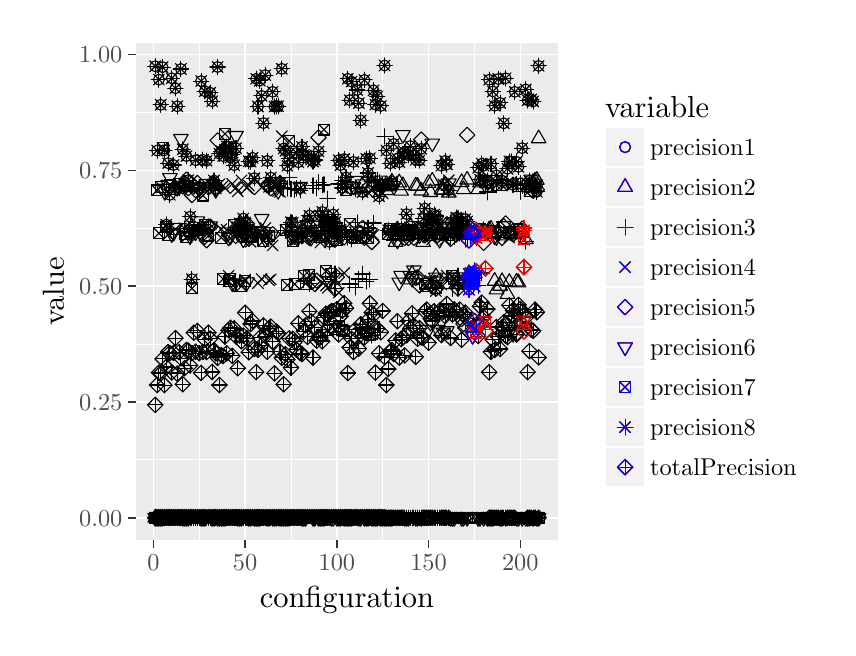
\begin{tikzpicture}[x=1pt,y=1pt]
\definecolor{fillColor}{RGB}{255,255,255}
\path[use as bounding box,fill=fillColor,fill opacity=0.00] (0,0) rectangle (289.08,216.81);
\begin{scope}
\path[clip] (  0.00,  0.00) rectangle (289.08,216.81);
\definecolor{drawColor}{RGB}{255,255,255}
\definecolor{fillColor}{RGB}{255,255,255}

\path[draw=drawColor,line width= 0.6pt,line join=round,line cap=round,fill=fillColor] (  0.00,  0.00) rectangle (289.08,216.81);
\end{scope}
\begin{scope}
\path[clip] ( 39.17, 31.53) rectangle (191.57,211.31);
\definecolor{fillColor}{gray}{0.92}

\path[fill=fillColor] ( 39.17, 31.53) rectangle (191.57,211.31);
\definecolor{drawColor}{RGB}{255,255,255}

\path[draw=drawColor,line width= 0.3pt,line join=round] ( 39.17, 60.63) --
	(191.57, 60.63);

\path[draw=drawColor,line width= 0.3pt,line join=round] ( 39.17,102.47) --
	(191.57,102.47);

\path[draw=drawColor,line width= 0.3pt,line join=round] ( 39.17,144.32) --
	(191.57,144.32);

\path[draw=drawColor,line width= 0.3pt,line join=round] ( 39.17,186.17) --
	(191.57,186.17);

\path[draw=drawColor,line width= 0.3pt,line join=round] ( 62.00, 31.53) --
	( 62.00,211.31);

\path[draw=drawColor,line width= 0.3pt,line join=round] ( 95.15, 31.53) --
	( 95.15,211.31);

\path[draw=drawColor,line width= 0.3pt,line join=round] (128.30, 31.53) --
	(128.30,211.31);

\path[draw=drawColor,line width= 0.3pt,line join=round] (161.44, 31.53) --
	(161.44,211.31);

\path[draw=drawColor,line width= 0.6pt,line join=round] ( 39.17, 39.70) --
	(191.57, 39.70);

\path[draw=drawColor,line width= 0.6pt,line join=round] ( 39.17, 81.55) --
	(191.57, 81.55);

\path[draw=drawColor,line width= 0.6pt,line join=round] ( 39.17,123.40) --
	(191.57,123.40);

\path[draw=drawColor,line width= 0.6pt,line join=round] ( 39.17,165.24) --
	(191.57,165.24);

\path[draw=drawColor,line width= 0.6pt,line join=round] ( 39.17,207.09) --
	(191.57,207.09);

\path[draw=drawColor,line width= 0.6pt,line join=round] ( 45.43, 31.53) --
	( 45.43,211.31);

\path[draw=drawColor,line width= 0.6pt,line join=round] ( 78.58, 31.53) --
	( 78.58,211.31);

\path[draw=drawColor,line width= 0.6pt,line join=round] (111.72, 31.53) --
	(111.72,211.31);

\path[draw=drawColor,line width= 0.6pt,line join=round] (144.87, 31.53) --
	(144.87,211.31);

\path[draw=drawColor,line width= 0.6pt,line join=round] (178.02, 31.53) --
	(178.02,211.31);
\definecolor{drawColor}{RGB}{0,0,0}

\path[draw=drawColor,line width= 0.4pt,line join=round,line cap=round] ( 46.09,202.87) circle (  1.96);

\path[draw=drawColor,line width= 0.4pt,line join=round,line cap=round] ( 46.76,172.41) circle (  1.96);

\path[draw=drawColor,line width= 0.4pt,line join=round,line cap=round] ( 47.42,198.05) circle (  1.96);

\path[draw=drawColor,line width= 0.4pt,line join=round,line cap=round] ( 48.08,188.94) circle (  1.96);

\path[draw=drawColor,line width= 0.4pt,line join=round,line cap=round] ( 48.75,202.54) circle (  1.96);

\path[draw=drawColor,line width= 0.4pt,line join=round,line cap=round] ( 49.41,172.47) circle (  1.96);

\path[draw=drawColor,line width= 0.4pt,line join=round,line cap=round] ( 50.07,145.62) circle (  1.96);

\path[draw=drawColor,line width= 0.4pt,line join=round,line cap=round] ( 50.73,167.85) circle (  1.96);

\path[draw=drawColor,line width= 0.4pt,line join=round,line cap=round] ( 51.40,156.40) circle (  1.96);

\path[draw=drawColor,line width= 0.4pt,line join=round,line cap=round] ( 52.06,198.52) circle (  1.96);

\path[draw=drawColor,line width= 0.4pt,line join=round,line cap=round] ( 52.72,167.18) circle (  1.96);

\path[draw=drawColor,line width= 0.4pt,line join=round,line cap=round] ( 53.39,194.90) circle (  1.96);

\path[draw=drawColor,line width= 0.4pt,line join=round,line cap=round] ( 54.05,188.41) circle (  1.96);

\path[draw=drawColor,line width= 0.4pt,line join=round,line cap=round] ( 54.71,158.95) circle (  1.96);

\path[draw=drawColor,line width= 0.4pt,line join=round,line cap=round] ( 55.38,201.87) circle (  1.96);

\path[draw=drawColor,line width= 0.4pt,line join=round,line cap=round] ( 56.04,172.87) circle (  1.96);

\path[draw=drawColor,line width= 0.4pt,line join=round,line cap=round] ( 56.70,144.22) circle (  1.96);

\path[draw=drawColor,line width= 0.4pt,line join=round,line cap=round] ( 57.36,170.40) circle (  1.96);

\path[draw=drawColor,line width= 0.4pt,line join=round,line cap=round] ( 58.03,161.69) circle (  1.96);

\path[draw=drawColor,line width= 0.4pt,line join=round,line cap=round] ( 58.69,148.50) circle (  1.96);

\path[draw=drawColor,line width= 0.4pt,line join=round,line cap=round] ( 59.35,125.94) circle (  1.96);

\path[draw=drawColor,line width= 0.4pt,line join=round,line cap=round] ( 60.02,143.21) circle (  1.96);

\path[draw=drawColor,line width= 0.4pt,line join=round,line cap=round] ( 60.68,168.92) circle (  1.96);

\path[draw=drawColor,line width= 0.4pt,line join=round,line cap=round] ( 61.34,143.75) circle (  1.96);

\path[draw=drawColor,line width= 0.4pt,line join=round,line cap=round] ( 62.00,158.88) circle (  1.96);

\path[draw=drawColor,line width= 0.4pt,line join=round,line cap=round] ( 62.67,197.51) circle (  1.96);

\path[draw=drawColor,line width= 0.4pt,line join=round,line cap=round] ( 63.33,169.06) circle (  1.96);

\path[draw=drawColor,line width= 0.4pt,line join=round,line cap=round] ( 63.99,193.83) circle (  1.96);

\path[draw=drawColor,line width= 0.4pt,line join=round,line cap=round] ( 64.66,168.72) circle (  1.96);

\path[draw=drawColor,line width= 0.4pt,line join=round,line cap=round] ( 65.32,143.82) circle (  1.96);

\path[draw=drawColor,line width= 0.4pt,line join=round,line cap=round] ( 65.98,193.30) circle (  1.96);

\path[draw=drawColor,line width= 0.4pt,line join=round,line cap=round] ( 66.65,190.22) circle (  1.96);

\path[draw=drawColor,line width= 0.4pt,line join=round,line cap=round] ( 67.31,161.56) circle (  1.96);

\path[draw=drawColor,line width= 0.4pt,line join=round,line cap=round] ( 67.97,158.75) circle (  1.96);

\path[draw=drawColor,line width= 0.4pt,line join=round,line cap=round] ( 68.63,202.60) circle (  1.96);

\path[draw=drawColor,line width= 0.4pt,line join=round,line cap=round] ( 69.30,171.27) circle (  1.96);

\path[draw=drawColor,line width= 0.4pt,line join=round,line cap=round] ( 69.96,172.14) circle (  1.96);

\path[draw=drawColor,line width= 0.4pt,line join=round,line cap=round] ( 70.62,170.40) circle (  1.96);

\path[draw=drawColor,line width= 0.4pt,line join=round,line cap=round] ( 71.29,172.74) circle (  1.96);

\path[draw=drawColor,line width= 0.4pt,line join=round,line cap=round] ( 71.95,173.88) circle (  1.96);

\path[draw=drawColor,line width= 0.4pt,line join=round,line cap=round] ( 72.61,173.81) circle (  1.96);

\path[draw=drawColor,line width= 0.4pt,line join=round,line cap=round] ( 73.27,169.86) circle (  1.96);

\path[draw=drawColor,line width= 0.4pt,line join=round,line cap=round] ( 73.94,171.07) circle (  1.96);

\path[draw=drawColor,line width= 0.4pt,line join=round,line cap=round] ( 74.60,167.12) circle (  1.96);

\path[draw=drawColor,line width= 0.4pt,line join=round,line cap=round] ( 75.26,173.28) circle (  1.96);

\path[draw=drawColor,line width= 0.4pt,line join=round,line cap=round] ( 75.93,144.69) circle (  1.96);

\path[draw=drawColor,line width= 0.4pt,line join=round,line cap=round] ( 76.59,146.09) circle (  1.96);

\path[draw=drawColor,line width= 0.4pt,line join=round,line cap=round] ( 77.25,140.94) circle (  1.96);

\path[draw=drawColor,line width= 0.4pt,line join=round,line cap=round] ( 77.91,147.83) circle (  1.96);

\path[draw=drawColor,line width= 0.4pt,line join=round,line cap=round] ( 78.58,146.43) circle (  1.96);

\path[draw=drawColor,line width= 0.4pt,line join=round,line cap=round] ( 79.24,143.75) circle (  1.96);

\path[draw=drawColor,line width= 0.4pt,line join=round,line cap=round] ( 79.90,168.52) circle (  1.96);

\path[draw=drawColor,line width= 0.4pt,line join=round,line cap=round] ( 80.57,168.39) circle (  1.96);

\path[draw=drawColor,line width= 0.4pt,line join=round,line cap=round] ( 81.23,169.79) circle (  1.96);

\path[draw=drawColor,line width= 0.4pt,line join=round,line cap=round] ( 81.89,162.43) circle (  1.96);

\path[draw=drawColor,line width= 0.4pt,line join=round,line cap=round] ( 82.56,198.32) circle (  1.96);

\path[draw=drawColor,line width= 0.4pt,line join=round,line cap=round] ( 83.22,188.34) circle (  1.96);

\path[draw=drawColor,line width= 0.4pt,line join=round,line cap=round] ( 83.88,197.65) circle (  1.96);

\path[draw=drawColor,line width= 0.4pt,line join=round,line cap=round] ( 84.54,192.16) circle (  1.96);

\path[draw=drawColor,line width= 0.4pt,line join=round,line cap=round] ( 85.21,182.32) circle (  1.96);

\path[draw=drawColor,line width= 0.4pt,line join=round,line cap=round] ( 85.87,199.66) circle (  1.96);

\path[draw=drawColor,line width= 0.4pt,line join=round,line cap=round] ( 86.53,168.66) circle (  1.96);

\path[draw=drawColor,line width= 0.4pt,line join=round,line cap=round] ( 87.20,159.28) circle (  1.96);

\path[draw=drawColor,line width= 0.4pt,line join=round,line cap=round] ( 87.86,162.63) circle (  1.96);

\path[draw=drawColor,line width= 0.4pt,line join=round,line cap=round] ( 88.52,193.63) circle (  1.96);

\path[draw=drawColor,line width= 0.4pt,line join=round,line cap=round] ( 89.18,188.27) circle (  1.96);

\path[draw=drawColor,line width= 0.4pt,line join=round,line cap=round] ( 89.85,188.48) circle (  1.96);

\path[draw=drawColor,line width= 0.4pt,line join=round,line cap=round] ( 90.51,188.41) circle (  1.96);

\path[draw=drawColor,line width= 0.4pt,line join=round,line cap=round] ( 91.17,160.49) circle (  1.96);

\path[draw=drawColor,line width= 0.4pt,line join=round,line cap=round] ( 91.84,201.93) circle (  1.96);

\path[draw=drawColor,line width= 0.4pt,line join=round,line cap=round] ( 92.50,173.14) circle (  1.96);

\path[draw=drawColor,line width= 0.4pt,line join=round,line cap=round] ( 93.16,172.34) circle (  1.96);

\path[draw=drawColor,line width= 0.4pt,line join=round,line cap=round] ( 93.83,166.92) circle (  1.96);

\path[draw=drawColor,line width= 0.4pt,line join=round,line cap=round] ( 94.49,169.39) circle (  1.96);

\path[draw=drawColor,line width= 0.4pt,line join=round,line cap=round] ( 95.15,146.49) circle (  1.96);

\path[draw=drawColor,line width= 0.4pt,line join=round,line cap=round] ( 95.81,146.29) circle (  1.96);

\path[draw=drawColor,line width= 0.4pt,line join=round,line cap=round] ( 96.48,141.21) circle (  1.96);

\path[draw=drawColor,line width= 0.4pt,line join=round,line cap=round] ( 97.14,171.54) circle (  1.96);

\path[draw=drawColor,line width= 0.4pt,line join=round,line cap=round] ( 97.80,168.19) circle (  1.96);

\path[draw=drawColor,line width= 0.4pt,line join=round,line cap=round] ( 98.47,158.75) circle (  1.96);

\path[draw=drawColor,line width= 0.4pt,line join=round,line cap=round] ( 99.13,173.75) circle (  1.96);

\path[draw=drawColor,line width= 0.4pt,line join=round,line cap=round] ( 99.79,170.80) circle (  1.96);

\path[draw=drawColor,line width= 0.4pt,line join=round,line cap=round] (100.45,170.60) circle (  1.96);

\path[draw=drawColor,line width= 0.4pt,line join=round,line cap=round] (101.12,146.96) circle (  1.96);

\path[draw=drawColor,line width= 0.4pt,line join=round,line cap=round] (101.78,148.91) circle (  1.96);

\path[draw=drawColor,line width= 0.4pt,line join=round,line cap=round] (102.44,169.19) circle (  1.96);

\path[draw=drawColor,line width= 0.4pt,line join=round,line cap=round] (103.11,168.46) circle (  1.96);

\path[draw=drawColor,line width= 0.4pt,line join=round,line cap=round] (103.77,168.99) circle (  1.96);

\path[draw=drawColor,line width= 0.4pt,line join=round,line cap=round] (104.43,141.61) circle (  1.96);

\path[draw=drawColor,line width= 0.4pt,line join=round,line cap=round] (105.09,172.07) circle (  1.96);

\path[draw=drawColor,line width= 0.4pt,line join=round,line cap=round] (105.76,148.91) circle (  1.96);

\path[draw=drawColor,line width= 0.4pt,line join=round,line cap=round] (106.42,150.24) circle (  1.96);

\path[draw=drawColor,line width= 0.4pt,line join=round,line cap=round] (107.08,146.83) circle (  1.96);

\path[draw=drawColor,line width= 0.4pt,line join=round,line cap=round] (107.75,145.56) circle (  1.96);

\path[draw=drawColor,line width= 0.4pt,line join=round,line cap=round] (108.41,146.96) circle (  1.96);

\path[draw=drawColor,line width= 0.4pt,line join=round,line cap=round] (109.07,139.40) circle (  1.96);

\path[draw=drawColor,line width= 0.4pt,line join=round,line cap=round] (109.74,146.63) circle (  1.96);

\path[draw=drawColor,line width= 0.4pt,line join=round,line cap=round] (110.40,149.31) circle (  1.96);

\path[draw=drawColor,line width= 0.4pt,line join=round,line cap=round] (111.06,146.49) circle (  1.96);

\path[draw=drawColor,line width= 0.4pt,line join=round,line cap=round] (111.72,142.81) circle (  1.96);

\path[draw=drawColor,line width= 0.4pt,line join=round,line cap=round] (112.39,168.92) circle (  1.96);

\path[draw=drawColor,line width= 0.4pt,line join=round,line cap=round] (113.05,167.12) circle (  1.96);

\path[draw=drawColor,line width= 0.4pt,line join=round,line cap=round] (113.71,158.88) circle (  1.96);

\path[draw=drawColor,line width= 0.4pt,line join=round,line cap=round] (114.38,169.33) circle (  1.96);

\path[draw=drawColor,line width= 0.4pt,line join=round,line cap=round] (115.04,162.70) circle (  1.96);

\path[draw=drawColor,line width= 0.4pt,line join=round,line cap=round] (115.70,198.32) circle (  1.96);

\path[draw=drawColor,line width= 0.4pt,line join=round,line cap=round] (116.36,190.62) circle (  1.96);

\path[draw=drawColor,line width= 0.4pt,line join=round,line cap=round] (117.03,197.31) circle (  1.96);

\path[draw=drawColor,line width= 0.4pt,line join=round,line cap=round] (117.69,168.32) circle (  1.96);

\path[draw=drawColor,line width= 0.4pt,line join=round,line cap=round] (118.35,158.55) circle (  1.96);

\path[draw=drawColor,line width= 0.4pt,line join=round,line cap=round] (119.02,194.30) circle (  1.96);

\path[draw=drawColor,line width= 0.4pt,line join=round,line cap=round] (119.68,189.55) circle (  1.96);

\path[draw=drawColor,line width= 0.4pt,line join=round,line cap=round] (120.34,183.32) circle (  1.96);

\path[draw=drawColor,line width= 0.4pt,line join=round,line cap=round] (121.01,157.41) circle (  1.96);

\path[draw=drawColor,line width= 0.4pt,line join=round,line cap=round] (121.67,197.92) circle (  1.96);

\path[draw=drawColor,line width= 0.4pt,line join=round,line cap=round] (122.33,169.39) circle (  1.96);

\path[draw=drawColor,line width= 0.4pt,line join=round,line cap=round] (122.99,164.30) circle (  1.96);

\path[draw=drawColor,line width= 0.4pt,line join=round,line cap=round] (123.66,169.59) circle (  1.96);

\path[draw=drawColor,line width= 0.4pt,line join=round,line cap=round] (124.32,161.22) circle (  1.96);

\path[draw=drawColor,line width= 0.4pt,line join=round,line cap=round] (124.98,194.17) circle (  1.96);

\path[draw=drawColor,line width= 0.4pt,line join=round,line cap=round] (125.65,189.01) circle (  1.96);

\path[draw=drawColor,line width= 0.4pt,line join=round,line cap=round] (126.31,191.89) circle (  1.96);

\path[draw=drawColor,line width= 0.4pt,line join=round,line cap=round] (126.97,155.87) circle (  1.96);

\path[draw=drawColor,line width= 0.4pt,line join=round,line cap=round] (127.63,188.54) circle (  1.96);

\path[draw=drawColor,line width= 0.4pt,line join=round,line cap=round] (128.30,160.09) circle (  1.96);

\path[draw=drawColor,line width= 0.4pt,line join=round,line cap=round] (128.96,203.14) circle (  1.96);

\path[draw=drawColor,line width= 0.4pt,line join=round,line cap=round] (129.62,172.41) circle (  1.96);

\path[draw=drawColor,line width= 0.4pt,line join=round,line cap=round] (130.29,143.62) circle (  1.96);

\path[draw=drawColor,line width= 0.4pt,line join=round,line cap=round] (130.95,167.79) circle (  1.96);

\path[draw=drawColor,line width= 0.4pt,line join=round,line cap=round] (131.61,161.22) circle (  1.96);

\path[draw=drawColor,line width= 0.4pt,line join=round,line cap=round] (132.28,174.82) circle (  1.96);

\path[draw=drawColor,line width= 0.4pt,line join=round,line cap=round] (132.94,143.35) circle (  1.96);

\path[draw=drawColor,line width= 0.4pt,line join=round,line cap=round] (133.60,169.46) circle (  1.96);

\path[draw=drawColor,line width= 0.4pt,line join=round,line cap=round] (134.26,168.19) circle (  1.96);

\path[draw=drawColor,line width= 0.4pt,line join=round,line cap=round] (134.93,144.15) circle (  1.96);

\path[draw=drawColor,line width= 0.4pt,line join=round,line cap=round] (135.59,171.20) circle (  1.96);

\path[draw=drawColor,line width= 0.4pt,line join=round,line cap=round] (136.25,171.87) circle (  1.96);

\path[draw=drawColor,line width= 0.4pt,line join=round,line cap=round] (136.92,149.44) circle (  1.96);

\path[draw=drawColor,line width= 0.4pt,line join=round,line cap=round] (137.58,170.73) circle (  1.96);

\path[draw=drawColor,line width= 0.4pt,line join=round,line cap=round] (138.24,174.01) circle (  1.96);

\path[draw=drawColor,line width= 0.4pt,line join=round,line cap=round] (138.90,143.68) circle (  1.96);

\path[draw=drawColor,line width= 0.4pt,line join=round,line cap=round] (139.57,170.80) circle (  1.96);

\path[draw=drawColor,line width= 0.4pt,line join=round,line cap=round] (140.23,169.06) circle (  1.96);

\path[draw=drawColor,line width= 0.4pt,line join=round,line cap=round] (140.89,143.68) circle (  1.96);

\path[draw=drawColor,line width= 0.4pt,line join=round,line cap=round] (141.56,168.86) circle (  1.96);

\path[draw=drawColor,line width= 0.4pt,line join=round,line cap=round] (142.22,173.01) circle (  1.96);

\path[draw=drawColor,line width= 0.4pt,line join=round,line cap=round] (142.88,147.70) circle (  1.96);

\path[draw=drawColor,line width= 0.4pt,line join=round,line cap=round] (143.54,151.45) circle (  1.96);

\path[draw=drawColor,line width= 0.4pt,line join=round,line cap=round] (144.21,142.28) circle (  1.96);

\path[draw=drawColor,line width= 0.4pt,line join=round,line cap=round] (144.87,146.29) circle (  1.96);

\path[draw=drawColor,line width= 0.4pt,line join=round,line cap=round] (145.53,147.50) circle (  1.96);

\path[draw=drawColor,line width= 0.4pt,line join=round,line cap=round] (146.20,145.36) circle (  1.96);

\path[draw=drawColor,line width= 0.4pt,line join=round,line cap=round] (146.86,149.24) circle (  1.96);

\path[draw=drawColor,line width= 0.4pt,line join=round,line cap=round] (147.52,148.77) circle (  1.96);

\path[draw=drawColor,line width= 0.4pt,line join=round,line cap=round] (148.19,146.29) circle (  1.96);

\path[draw=drawColor,line width= 0.4pt,line join=round,line cap=round] (148.85,142.41) circle (  1.96);

\path[draw=drawColor,line width= 0.4pt,line join=round,line cap=round] (149.51,166.92) circle (  1.96);

\path[draw=drawColor,line width= 0.4pt,line join=round,line cap=round] (150.17,160.15) circle (  1.96);

\path[draw=drawColor,line width= 0.4pt,line join=round,line cap=round] (150.84,168.66) circle (  1.96);

\path[draw=drawColor,line width= 0.4pt,line join=round,line cap=round] (151.50,167.38) circle (  1.96);

\path[draw=drawColor,line width= 0.4pt,line join=round,line cap=round] (152.16,158.08) circle (  1.96);

\path[draw=drawColor,line width= 0.4pt,line join=round,line cap=round] (152.83,146.36) circle (  1.96);

\path[draw=drawColor,line width= 0.4pt,line join=round,line cap=round] (153.49,144.62) circle (  1.96);

\path[draw=drawColor,line width= 0.4pt,line join=round,line cap=round] (154.15,142.81) circle (  1.96);

\path[draw=drawColor,line width= 0.4pt,line join=round,line cap=round] (154.81,148.17) circle (  1.96);

\path[draw=drawColor,line width= 0.4pt,line join=round,line cap=round] (155.48,147.90) circle (  1.96);

\path[draw=drawColor,line width= 0.4pt,line join=round,line cap=round] (156.14,142.48) circle (  1.96);

\path[draw=drawColor,line width= 0.4pt,line join=round,line cap=round] (156.80,146.76) circle (  1.96);

\path[draw=drawColor,line width= 0.4pt,line join=round,line cap=round] (157.47,145.42) circle (  1.96);

\path[draw=drawColor,line width= 0.4pt,line join=round,line cap=round] (158.13,147.63) circle (  1.96);

\path[draw=drawColor,line width= 0.4pt,line join=round,line cap=round] (158.79,146.76) circle (  1.96);

\path[draw=drawColor,line width= 0.4pt,line join=round,line cap=round] (159.46,122.19) circle (  1.96);

\path[draw=drawColor,line width= 0.4pt,line join=round,line cap=round] (160.12,125.81) circle (  1.96);

\path[draw=drawColor,line width= 0.4pt,line join=round,line cap=round] (160.78,127.14) circle (  1.96);

\path[draw=drawColor,line width= 0.4pt,line join=round,line cap=round] (161.44,126.48) circle (  1.96);

\path[draw=drawColor,line width= 0.4pt,line join=round,line cap=round] (162.11,140.80) circle (  1.96);

\path[draw=drawColor,line width= 0.4pt,line join=round,line cap=round] (162.77,166.18) circle (  1.96);

\path[draw=drawColor,line width= 0.4pt,line join=round,line cap=round] (163.43,161.89) circle (  1.96);

\path[draw=drawColor,line width= 0.4pt,line join=round,line cap=round] (164.10,167.65) circle (  1.96);

\path[draw=drawColor,line width= 0.4pt,line join=round,line cap=round] (164.76,166.92) circle (  1.96);

\path[draw=drawColor,line width= 0.4pt,line join=round,line cap=round] (165.42,142.68) circle (  1.96);

\path[draw=drawColor,line width= 0.4pt,line join=round,line cap=round] (166.08,161.56) circle (  1.96);

\path[draw=drawColor,line width= 0.4pt,line join=round,line cap=round] (166.75,197.98) circle (  1.96);

\path[draw=drawColor,line width= 0.4pt,line join=round,line cap=round] (167.41,167.59) circle (  1.96);

\path[draw=drawColor,line width= 0.4pt,line join=round,line cap=round] (168.07,193.76) circle (  1.96);

\path[draw=drawColor,line width= 0.4pt,line join=round,line cap=round] (168.74,188.61) circle (  1.96);

\path[draw=drawColor,line width= 0.4pt,line join=round,line cap=round] (169.40,163.43) circle (  1.96);

\path[draw=drawColor,line width= 0.4pt,line join=round,line cap=round] (170.06,198.25) circle (  1.96);

\path[draw=drawColor,line width= 0.4pt,line join=round,line cap=round] (170.73,189.61) circle (  1.96);

\path[draw=drawColor,line width= 0.4pt,line join=round,line cap=round] (171.39,161.49) circle (  1.96);

\path[draw=drawColor,line width= 0.4pt,line join=round,line cap=round] (172.05,182.25) circle (  1.96);

\path[draw=drawColor,line width= 0.4pt,line join=round,line cap=round] (172.71,198.52) circle (  1.96);

\path[draw=drawColor,line width= 0.4pt,line join=round,line cap=round] (173.38,165.84) circle (  1.96);

\path[draw=drawColor,line width= 0.4pt,line join=round,line cap=round] (174.04,168.46) circle (  1.96);

\path[draw=drawColor,line width= 0.4pt,line join=round,line cap=round] (174.70,168.46) circle (  1.96);

\path[draw=drawColor,line width= 0.4pt,line join=round,line cap=round] (175.37,160.02) circle (  1.96);

\path[draw=drawColor,line width= 0.4pt,line join=round,line cap=round] (176.03,193.63) circle (  1.96);

\path[draw=drawColor,line width= 0.4pt,line join=round,line cap=round] (176.69,168.32) circle (  1.96);

\path[draw=drawColor,line width= 0.4pt,line join=round,line cap=round] (177.35,166.51) circle (  1.96);

\path[draw=drawColor,line width= 0.4pt,line join=round,line cap=round] (178.02,160.56) circle (  1.96);

\path[draw=drawColor,line width= 0.4pt,line join=round,line cap=round] (178.68,173.28) circle (  1.96);

\path[draw=drawColor,line width= 0.4pt,line join=round,line cap=round] (179.34,143.41) circle (  1.96);

\path[draw=drawColor,line width= 0.4pt,line join=round,line cap=round] (180.01,194.50) circle (  1.96);

\path[draw=drawColor,line width= 0.4pt,line join=round,line cap=round] (180.67,190.55) circle (  1.96);

\path[draw=drawColor,line width= 0.4pt,line join=round,line cap=round] (181.33,161.49) circle (  1.96);

\path[draw=drawColor,line width= 0.4pt,line join=round,line cap=round] (181.99,190.89) circle (  1.96);

\path[draw=drawColor,line width= 0.4pt,line join=round,line cap=round] (182.66,190.15) circle (  1.96);

\path[draw=drawColor,line width= 0.4pt,line join=round,line cap=round] (183.32,159.55) circle (  1.96);

\path[draw=drawColor,line width= 0.4pt,line join=round,line cap=round] (183.98,157.54) circle (  1.96);

\path[draw=drawColor,line width= 0.4pt,line join=round,line cap=round] (184.65,203.00) circle (  1.96);

\path[draw=drawColor,line width= 0.4pt,line join=round,line cap=round] ( 46.09, 42.75) --
	( 48.74, 38.18) --
	( 43.45, 38.18) --
	( 46.09, 42.75);

\path[draw=drawColor,line width= 0.4pt,line join=round,line cap=round] ( 46.76, 42.75) --
	( 49.40, 38.18) --
	( 44.11, 38.18) --
	( 46.76, 42.75);

\path[draw=drawColor,line width= 0.4pt,line join=round,line cap=round] ( 47.42, 42.75) --
	( 50.06, 38.18) --
	( 44.78, 38.18) --
	( 47.42, 42.75);

\path[draw=drawColor,line width= 0.4pt,line join=round,line cap=round] ( 48.08, 42.75) --
	( 50.73, 38.18) --
	( 45.44, 38.18) --
	( 48.08, 42.75);

\path[draw=drawColor,line width= 0.4pt,line join=round,line cap=round] ( 48.75, 42.75) --
	( 51.39, 38.18) --
	( 46.10, 38.18) --
	( 48.75, 42.75);

\path[draw=drawColor,line width= 0.4pt,line join=round,line cap=round] ( 49.41, 42.75) --
	( 52.05, 38.18) --
	( 46.77, 38.18) --
	( 49.41, 42.75);

\path[draw=drawColor,line width= 0.4pt,line join=round,line cap=round] ( 50.07, 42.75) --
	( 52.71, 38.18) --
	( 47.43, 38.18) --
	( 50.07, 42.75);

\path[draw=drawColor,line width= 0.4pt,line join=round,line cap=round] ( 50.73, 42.75) --
	( 53.38, 38.18) --
	( 48.09, 38.18) --
	( 50.73, 42.75);

\path[draw=drawColor,line width= 0.4pt,line join=round,line cap=round] ( 51.40, 42.75) --
	( 54.04, 38.18) --
	( 48.76, 38.18) --
	( 51.40, 42.75);

\path[draw=drawColor,line width= 0.4pt,line join=round,line cap=round] ( 52.06, 42.75) --
	( 54.70, 38.18) --
	( 49.42, 38.18) --
	( 52.06, 42.75);

\path[draw=drawColor,line width= 0.4pt,line join=round,line cap=round] ( 52.72, 42.75) --
	( 55.37, 38.18) --
	( 50.08, 38.18) --
	( 52.72, 42.75);

\path[draw=drawColor,line width= 0.4pt,line join=round,line cap=round] ( 53.39, 42.75) --
	( 56.03, 38.18) --
	( 50.74, 38.18) --
	( 53.39, 42.75);

\path[draw=drawColor,line width= 0.4pt,line join=round,line cap=round] ( 54.05, 42.75) --
	( 56.69, 38.18) --
	( 51.41, 38.18) --
	( 54.05, 42.75);

\path[draw=drawColor,line width= 0.4pt,line join=round,line cap=round] ( 54.71, 42.75) --
	( 57.35, 38.18) --
	( 52.07, 38.18) --
	( 54.71, 42.75);

\path[draw=drawColor,line width= 0.4pt,line join=round,line cap=round] ( 55.38, 42.75) --
	( 58.02, 38.18) --
	( 52.73, 38.18) --
	( 55.38, 42.75);

\path[draw=drawColor,line width= 0.4pt,line join=round,line cap=round] ( 56.04, 42.75) --
	( 58.68, 38.18) --
	( 53.40, 38.18) --
	( 56.04, 42.75);

\path[draw=drawColor,line width= 0.4pt,line join=round,line cap=round] ( 56.70, 42.75) --
	( 59.34, 38.18) --
	( 54.06, 38.18) --
	( 56.70, 42.75);

\path[draw=drawColor,line width= 0.4pt,line join=round,line cap=round] ( 57.36, 42.75) --
	( 60.01, 38.18) --
	( 54.72, 38.18) --
	( 57.36, 42.75);

\path[draw=drawColor,line width= 0.4pt,line join=round,line cap=round] ( 58.03, 42.75) --
	( 60.67, 38.18) --
	( 55.38, 38.18) --
	( 58.03, 42.75);

\path[draw=drawColor,line width= 0.4pt,line join=round,line cap=round] ( 58.69, 42.75) --
	( 61.33, 38.18) --
	( 56.05, 38.18) --
	( 58.69, 42.75);

\path[draw=drawColor,line width= 0.4pt,line join=round,line cap=round] ( 59.35, 42.75) --
	( 62.00, 38.18) --
	( 56.71, 38.18) --
	( 59.35, 42.75);

\path[draw=drawColor,line width= 0.4pt,line join=round,line cap=round] ( 60.02, 42.75) --
	( 62.66, 38.18) --
	( 57.37, 38.18) --
	( 60.02, 42.75);

\path[draw=drawColor,line width= 0.4pt,line join=round,line cap=round] ( 60.68, 42.75) --
	( 63.32, 38.18) --
	( 58.04, 38.18) --
	( 60.68, 42.75);

\path[draw=drawColor,line width= 0.4pt,line join=round,line cap=round] ( 61.34, 42.75) --
	( 63.98, 38.18) --
	( 58.70, 38.18) --
	( 61.34, 42.75);

\path[draw=drawColor,line width= 0.4pt,line join=round,line cap=round] ( 62.00, 42.75) --
	( 64.65, 38.18) --
	( 59.36, 38.18) --
	( 62.00, 42.75);

\path[draw=drawColor,line width= 0.4pt,line join=round,line cap=round] ( 62.67, 42.75) --
	( 65.31, 38.18) --
	( 60.02, 38.18) --
	( 62.67, 42.75);

\path[draw=drawColor,line width= 0.4pt,line join=round,line cap=round] ( 63.33, 42.75) --
	( 65.97, 38.18) --
	( 60.69, 38.18) --
	( 63.33, 42.75);

\path[draw=drawColor,line width= 0.4pt,line join=round,line cap=round] ( 63.99, 42.75) --
	( 66.64, 38.18) --
	( 61.35, 38.18) --
	( 63.99, 42.75);

\path[draw=drawColor,line width= 0.4pt,line join=round,line cap=round] ( 64.66, 42.75) --
	( 67.30, 38.18) --
	( 62.01, 38.18) --
	( 64.66, 42.75);

\path[draw=drawColor,line width= 0.4pt,line join=round,line cap=round] ( 65.32, 42.75) --
	( 67.96, 38.18) --
	( 62.68, 38.18) --
	( 65.32, 42.75);

\path[draw=drawColor,line width= 0.4pt,line join=round,line cap=round] ( 65.98, 42.75) --
	( 68.62, 38.18) --
	( 63.34, 38.18) --
	( 65.98, 42.75);

\path[draw=drawColor,line width= 0.4pt,line join=round,line cap=round] ( 66.65, 42.75) --
	( 69.29, 38.18) --
	( 64.00, 38.18) --
	( 66.65, 42.75);

\path[draw=drawColor,line width= 0.4pt,line join=round,line cap=round] ( 67.31, 42.75) --
	( 69.95, 38.18) --
	( 64.67, 38.18) --
	( 67.31, 42.75);

\path[draw=drawColor,line width= 0.4pt,line join=round,line cap=round] ( 67.97, 42.75) --
	( 70.61, 38.18) --
	( 65.33, 38.18) --
	( 67.97, 42.75);

\path[draw=drawColor,line width= 0.4pt,line join=round,line cap=round] ( 68.63, 42.75) --
	( 71.28, 38.18) --
	( 65.99, 38.18) --
	( 68.63, 42.75);

\path[draw=drawColor,line width= 0.4pt,line join=round,line cap=round] ( 69.30, 42.75) --
	( 71.94, 38.18) --
	( 66.65, 38.18) --
	( 69.30, 42.75);

\path[draw=drawColor,line width= 0.4pt,line join=round,line cap=round] ( 69.96, 42.75) --
	( 72.60, 38.18) --
	( 67.32, 38.18) --
	( 69.96, 42.75);

\path[draw=drawColor,line width= 0.4pt,line join=round,line cap=round] ( 70.62, 42.75) --
	( 73.27, 38.18) --
	( 67.98, 38.18) --
	( 70.62, 42.75);

\path[draw=drawColor,line width= 0.4pt,line join=round,line cap=round] ( 71.29, 42.75) --
	( 73.93, 38.18) --
	( 68.64, 38.18) --
	( 71.29, 42.75);

\path[draw=drawColor,line width= 0.4pt,line join=round,line cap=round] ( 71.95, 42.75) --
	( 74.59, 38.18) --
	( 69.31, 38.18) --
	( 71.95, 42.75);

\path[draw=drawColor,line width= 0.4pt,line join=round,line cap=round] ( 72.61, 42.75) --
	( 75.25, 38.18) --
	( 69.97, 38.18) --
	( 72.61, 42.75);

\path[draw=drawColor,line width= 0.4pt,line join=round,line cap=round] ( 73.27, 42.75) --
	( 75.92, 38.18) --
	( 70.63, 38.18) --
	( 73.27, 42.75);

\path[draw=drawColor,line width= 0.4pt,line join=round,line cap=round] ( 73.94, 42.75) --
	( 76.58, 38.18) --
	( 71.29, 38.18) --
	( 73.94, 42.75);

\path[draw=drawColor,line width= 0.4pt,line join=round,line cap=round] ( 74.60, 42.75) --
	( 77.24, 38.18) --
	( 71.96, 38.18) --
	( 74.60, 42.75);

\path[draw=drawColor,line width= 0.4pt,line join=round,line cap=round] ( 75.26, 42.75) --
	( 77.91, 38.18) --
	( 72.62, 38.18) --
	( 75.26, 42.75);

\path[draw=drawColor,line width= 0.4pt,line join=round,line cap=round] ( 75.93, 42.75) --
	( 78.57, 38.18) --
	( 73.28, 38.18) --
	( 75.93, 42.75);

\path[draw=drawColor,line width= 0.4pt,line join=round,line cap=round] ( 76.59, 42.75) --
	( 79.23, 38.18) --
	( 73.95, 38.18) --
	( 76.59, 42.75);

\path[draw=drawColor,line width= 0.4pt,line join=round,line cap=round] ( 77.25, 42.75) --
	( 79.89, 38.18) --
	( 74.61, 38.18) --
	( 77.25, 42.75);

\path[draw=drawColor,line width= 0.4pt,line join=round,line cap=round] ( 77.91, 42.75) --
	( 80.56, 38.18) --
	( 75.27, 38.18) --
	( 77.91, 42.75);

\path[draw=drawColor,line width= 0.4pt,line join=round,line cap=round] ( 78.58, 42.75) --
	( 81.22, 38.18) --
	( 75.94, 38.18) --
	( 78.58, 42.75);

\path[draw=drawColor,line width= 0.4pt,line join=round,line cap=round] ( 79.24, 42.75) --
	( 81.88, 38.18) --
	( 76.60, 38.18) --
	( 79.24, 42.75);

\path[draw=drawColor,line width= 0.4pt,line join=round,line cap=round] ( 79.90, 42.75) --
	( 82.55, 38.18) --
	( 77.26, 38.18) --
	( 79.90, 42.75);

\path[draw=drawColor,line width= 0.4pt,line join=round,line cap=round] ( 80.57, 42.75) --
	( 83.21, 38.18) --
	( 77.92, 38.18) --
	( 80.57, 42.75);

\path[draw=drawColor,line width= 0.4pt,line join=round,line cap=round] ( 81.23, 42.75) --
	( 83.87, 38.18) --
	( 78.59, 38.18) --
	( 81.23, 42.75);

\path[draw=drawColor,line width= 0.4pt,line join=round,line cap=round] ( 81.89, 42.75) --
	( 84.54, 38.18) --
	( 79.25, 38.18) --
	( 81.89, 42.75);

\path[draw=drawColor,line width= 0.4pt,line join=round,line cap=round] ( 82.56, 42.75) --
	( 85.20, 38.18) --
	( 79.91, 38.18) --
	( 82.56, 42.75);

\path[draw=drawColor,line width= 0.4pt,line join=round,line cap=round] ( 83.22, 42.75) --
	( 85.86, 38.18) --
	( 80.58, 38.18) --
	( 83.22, 42.75);

\path[draw=drawColor,line width= 0.4pt,line join=round,line cap=round] ( 83.88, 42.75) --
	( 86.52, 38.18) --
	( 81.24, 38.18) --
	( 83.88, 42.75);

\path[draw=drawColor,line width= 0.4pt,line join=round,line cap=round] ( 84.54, 42.75) --
	( 87.19, 38.18) --
	( 81.90, 38.18) --
	( 84.54, 42.75);

\path[draw=drawColor,line width= 0.4pt,line join=round,line cap=round] ( 85.21, 42.75) --
	( 87.85, 38.18) --
	( 82.56, 38.18) --
	( 85.21, 42.75);

\path[draw=drawColor,line width= 0.4pt,line join=round,line cap=round] ( 85.87, 42.75) --
	( 88.51, 38.18) --
	( 83.23, 38.18) --
	( 85.87, 42.75);

\path[draw=drawColor,line width= 0.4pt,line join=round,line cap=round] ( 86.53, 42.75) --
	( 89.18, 38.18) --
	( 83.89, 38.18) --
	( 86.53, 42.75);

\path[draw=drawColor,line width= 0.4pt,line join=round,line cap=round] ( 87.20, 42.75) --
	( 89.84, 38.18) --
	( 84.55, 38.18) --
	( 87.20, 42.75);

\path[draw=drawColor,line width= 0.4pt,line join=round,line cap=round] ( 87.86, 42.75) --
	( 90.50, 38.18) --
	( 85.22, 38.18) --
	( 87.86, 42.75);

\path[draw=drawColor,line width= 0.4pt,line join=round,line cap=round] ( 88.52, 42.75) --
	( 91.16, 38.18) --
	( 85.88, 38.18) --
	( 88.52, 42.75);

\path[draw=drawColor,line width= 0.4pt,line join=round,line cap=round] ( 89.18, 42.75) --
	( 91.83, 38.18) --
	( 86.54, 38.18) --
	( 89.18, 42.75);

\path[draw=drawColor,line width= 0.4pt,line join=round,line cap=round] ( 89.85, 42.75) --
	( 92.49, 38.18) --
	( 87.21, 38.18) --
	( 89.85, 42.75);

\path[draw=drawColor,line width= 0.4pt,line join=round,line cap=round] ( 90.51, 42.75) --
	( 93.15, 38.18) --
	( 87.87, 38.18) --
	( 90.51, 42.75);

\path[draw=drawColor,line width= 0.4pt,line join=round,line cap=round] ( 91.17, 42.75) --
	( 93.82, 38.18) --
	( 88.53, 38.18) --
	( 91.17, 42.75);

\path[draw=drawColor,line width= 0.4pt,line join=round,line cap=round] ( 91.84, 42.75) --
	( 94.48, 38.18) --
	( 89.19, 38.18) --
	( 91.84, 42.75);

\path[draw=drawColor,line width= 0.4pt,line join=round,line cap=round] ( 92.50, 42.75) --
	( 95.14, 38.18) --
	( 89.86, 38.18) --
	( 92.50, 42.75);

\path[draw=drawColor,line width= 0.4pt,line join=round,line cap=round] ( 93.16, 42.75) --
	( 95.80, 38.18) --
	( 90.52, 38.18) --
	( 93.16, 42.75);

\path[draw=drawColor,line width= 0.4pt,line join=round,line cap=round] ( 93.83, 42.75) --
	( 96.47, 38.18) --
	( 91.18, 38.18) --
	( 93.83, 42.75);

\path[draw=drawColor,line width= 0.4pt,line join=round,line cap=round] ( 94.49, 42.75) --
	( 97.13, 38.18) --
	( 91.85, 38.18) --
	( 94.49, 42.75);

\path[draw=drawColor,line width= 0.4pt,line join=round,line cap=round] ( 95.15, 42.75) --
	( 97.79, 38.18) --
	( 92.51, 38.18) --
	( 95.15, 42.75);

\path[draw=drawColor,line width= 0.4pt,line join=round,line cap=round] ( 95.81, 42.75) --
	( 98.46, 38.18) --
	( 93.17, 38.18) --
	( 95.81, 42.75);

\path[draw=drawColor,line width= 0.4pt,line join=round,line cap=round] ( 96.48, 42.75) --
	( 99.12, 38.18) --
	( 93.83, 38.18) --
	( 96.48, 42.75);

\path[draw=drawColor,line width= 0.4pt,line join=round,line cap=round] ( 97.14, 42.75) --
	( 99.78, 38.18) --
	( 94.50, 38.18) --
	( 97.14, 42.75);

\path[draw=drawColor,line width= 0.4pt,line join=round,line cap=round] ( 97.80, 42.75) --
	(100.45, 38.18) --
	( 95.16, 38.18) --
	( 97.80, 42.75);

\path[draw=drawColor,line width= 0.4pt,line join=round,line cap=round] ( 98.47, 42.75) --
	(101.11, 38.18) --
	( 95.82, 38.18) --
	( 98.47, 42.75);

\path[draw=drawColor,line width= 0.4pt,line join=round,line cap=round] ( 99.13, 42.75) --
	(101.77, 38.18) --
	( 96.49, 38.18) --
	( 99.13, 42.75);

\path[draw=drawColor,line width= 0.4pt,line join=round,line cap=round] ( 99.79, 42.75) --
	(102.43, 38.18) --
	( 97.15, 38.18) --
	( 99.79, 42.75);

\path[draw=drawColor,line width= 0.4pt,line join=round,line cap=round] (100.45, 42.75) --
	(103.10, 38.18) --
	( 97.81, 38.18) --
	(100.45, 42.75);

\path[draw=drawColor,line width= 0.4pt,line join=round,line cap=round] (101.12, 42.75) --
	(103.76, 38.18) --
	( 98.47, 38.18) --
	(101.12, 42.75);

\path[draw=drawColor,line width= 0.4pt,line join=round,line cap=round] (101.78, 42.75) --
	(104.42, 38.18) --
	( 99.14, 38.18) --
	(101.78, 42.75);

\path[draw=drawColor,line width= 0.4pt,line join=round,line cap=round] (102.44, 42.75) --
	(105.09, 38.18) --
	( 99.80, 38.18) --
	(102.44, 42.75);

\path[draw=drawColor,line width= 0.4pt,line join=round,line cap=round] (103.11, 42.75) --
	(105.75, 38.18) --
	(100.46, 38.18) --
	(103.11, 42.75);

\path[draw=drawColor,line width= 0.4pt,line join=round,line cap=round] (103.77, 42.75) --
	(106.41, 38.18) --
	(101.13, 38.18) --
	(103.77, 42.75);

\path[draw=drawColor,line width= 0.4pt,line join=round,line cap=round] (104.43, 42.75) --
	(107.07, 38.18) --
	(101.79, 38.18) --
	(104.43, 42.75);

\path[draw=drawColor,line width= 0.4pt,line join=round,line cap=round] (105.09, 42.75) --
	(107.74, 38.18) --
	(102.45, 38.18) --
	(105.09, 42.75);

\path[draw=drawColor,line width= 0.4pt,line join=round,line cap=round] (105.76, 42.75) --
	(108.40, 38.18) --
	(103.12, 38.18) --
	(105.76, 42.75);

\path[draw=drawColor,line width= 0.4pt,line join=round,line cap=round] (106.42, 42.75) --
	(109.06, 38.18) --
	(103.78, 38.18) --
	(106.42, 42.75);

\path[draw=drawColor,line width= 0.4pt,line join=round,line cap=round] (107.08, 42.75) --
	(109.73, 38.18) --
	(104.44, 38.18) --
	(107.08, 42.75);

\path[draw=drawColor,line width= 0.4pt,line join=round,line cap=round] (107.75, 42.75) --
	(110.39, 38.18) --
	(105.10, 38.18) --
	(107.75, 42.75);

\path[draw=drawColor,line width= 0.4pt,line join=round,line cap=round] (108.41, 42.75) --
	(111.05, 38.18) --
	(105.77, 38.18) --
	(108.41, 42.75);

\path[draw=drawColor,line width= 0.4pt,line join=round,line cap=round] (109.07, 42.75) --
	(111.72, 38.18) --
	(106.43, 38.18) --
	(109.07, 42.75);

\path[draw=drawColor,line width= 0.4pt,line join=round,line cap=round] (109.74, 42.75) --
	(112.38, 38.18) --
	(107.09, 38.18) --
	(109.74, 42.75);

\path[draw=drawColor,line width= 0.4pt,line join=round,line cap=round] (110.40, 42.75) --
	(113.04, 38.18) --
	(107.76, 38.18) --
	(110.40, 42.75);

\path[draw=drawColor,line width= 0.4pt,line join=round,line cap=round] (111.06, 42.75) --
	(113.70, 38.18) --
	(108.42, 38.18) --
	(111.06, 42.75);

\path[draw=drawColor,line width= 0.4pt,line join=round,line cap=round] (111.72, 42.75) --
	(114.37, 38.18) --
	(109.08, 38.18) --
	(111.72, 42.75);

\path[draw=drawColor,line width= 0.4pt,line join=round,line cap=round] (112.39, 42.75) --
	(115.03, 38.18) --
	(109.74, 38.18) --
	(112.39, 42.75);

\path[draw=drawColor,line width= 0.4pt,line join=round,line cap=round] (113.05, 42.75) --
	(115.69, 38.18) --
	(110.41, 38.18) --
	(113.05, 42.75);

\path[draw=drawColor,line width= 0.4pt,line join=round,line cap=round] (113.71, 42.75) --
	(116.36, 38.18) --
	(111.07, 38.18) --
	(113.71, 42.75);

\path[draw=drawColor,line width= 0.4pt,line join=round,line cap=round] (114.38, 42.75) --
	(117.02, 38.18) --
	(111.73, 38.18) --
	(114.38, 42.75);

\path[draw=drawColor,line width= 0.4pt,line join=round,line cap=round] (115.04, 42.75) --
	(117.68, 38.18) --
	(112.40, 38.18) --
	(115.04, 42.75);

\path[draw=drawColor,line width= 0.4pt,line join=round,line cap=round] (115.70, 42.75) --
	(118.34, 38.18) --
	(113.06, 38.18) --
	(115.70, 42.75);

\path[draw=drawColor,line width= 0.4pt,line join=round,line cap=round] (116.36, 42.75) --
	(119.01, 38.18) --
	(113.72, 38.18) --
	(116.36, 42.75);

\path[draw=drawColor,line width= 0.4pt,line join=round,line cap=round] (117.03, 42.75) --
	(119.67, 38.18) --
	(114.39, 38.18) --
	(117.03, 42.75);

\path[draw=drawColor,line width= 0.4pt,line join=round,line cap=round] (117.69, 42.75) --
	(120.33, 38.18) --
	(115.05, 38.18) --
	(117.69, 42.75);

\path[draw=drawColor,line width= 0.4pt,line join=round,line cap=round] (118.35, 42.75) --
	(121.00, 38.18) --
	(115.71, 38.18) --
	(118.35, 42.75);

\path[draw=drawColor,line width= 0.4pt,line join=round,line cap=round] (119.02, 42.75) --
	(121.66, 38.18) --
	(116.37, 38.18) --
	(119.02, 42.75);

\path[draw=drawColor,line width= 0.4pt,line join=round,line cap=round] (119.68, 42.75) --
	(122.32, 38.18) --
	(117.04, 38.18) --
	(119.68, 42.75);

\path[draw=drawColor,line width= 0.4pt,line join=round,line cap=round] (120.34, 42.75) --
	(122.98, 38.18) --
	(117.70, 38.18) --
	(120.34, 42.75);

\path[draw=drawColor,line width= 0.4pt,line join=round,line cap=round] (121.01, 42.75) --
	(123.65, 38.18) --
	(118.36, 38.18) --
	(121.01, 42.75);

\path[draw=drawColor,line width= 0.4pt,line join=round,line cap=round] (121.67, 42.75) --
	(124.31, 38.18) --
	(119.03, 38.18) --
	(121.67, 42.75);

\path[draw=drawColor,line width= 0.4pt,line join=round,line cap=round] (122.33, 42.75) --
	(124.97, 38.18) --
	(119.69, 38.18) --
	(122.33, 42.75);

\path[draw=drawColor,line width= 0.4pt,line join=round,line cap=round] (122.99, 42.75) --
	(125.64, 38.18) --
	(120.35, 38.18) --
	(122.99, 42.75);

\path[draw=drawColor,line width= 0.4pt,line join=round,line cap=round] (123.66, 42.75) --
	(126.30, 38.18) --
	(121.01, 38.18) --
	(123.66, 42.75);

\path[draw=drawColor,line width= 0.4pt,line join=round,line cap=round] (124.32, 42.75) --
	(126.96, 38.18) --
	(121.68, 38.18) --
	(124.32, 42.75);

\path[draw=drawColor,line width= 0.4pt,line join=round,line cap=round] (124.98, 42.75) --
	(127.63, 38.18) --
	(122.34, 38.18) --
	(124.98, 42.75);

\path[draw=drawColor,line width= 0.4pt,line join=round,line cap=round] (125.65, 42.75) --
	(128.29, 38.18) --
	(123.00, 38.18) --
	(125.65, 42.75);

\path[draw=drawColor,line width= 0.4pt,line join=round,line cap=round] (126.31, 42.75) --
	(128.95, 38.18) --
	(123.67, 38.18) --
	(126.31, 42.75);

\path[draw=drawColor,line width= 0.4pt,line join=round,line cap=round] (126.97, 42.75) --
	(129.61, 38.18) --
	(124.33, 38.18) --
	(126.97, 42.75);

\path[draw=drawColor,line width= 0.4pt,line join=round,line cap=round] (127.63, 42.75) --
	(130.28, 38.18) --
	(124.99, 38.18) --
	(127.63, 42.75);

\path[draw=drawColor,line width= 0.4pt,line join=round,line cap=round] (128.30, 42.75) --
	(130.94, 38.18) --
	(125.65, 38.18) --
	(128.30, 42.75);

\path[draw=drawColor,line width= 0.4pt,line join=round,line cap=round] (128.96, 42.75) --
	(131.60, 38.18) --
	(126.32, 38.18) --
	(128.96, 42.75);

\path[draw=drawColor,line width= 0.4pt,line join=round,line cap=round] (129.62,161.06) --
	(132.27,156.49) --
	(126.98,156.49) --
	(129.62,161.06);

\path[draw=drawColor,line width= 0.4pt,line join=round,line cap=round] (130.29,162.47) --
	(132.93,157.89) --
	(127.64,157.89) --
	(130.29,162.47);

\path[draw=drawColor,line width= 0.4pt,line join=round,line cap=round] (130.95,163.27) --
	(133.59,158.69) --
	(128.31,158.69) --
	(130.95,163.27);

\path[draw=drawColor,line width= 0.4pt,line join=round,line cap=round] (131.61,164.14) --
	(134.25,159.57) --
	(128.97,159.57) --
	(131.61,164.14);

\path[draw=drawColor,line width= 0.4pt,line join=round,line cap=round] (132.28,144.52) --
	(134.92,139.95) --
	(129.63,139.95) --
	(132.28,144.52);

\path[draw=drawColor,line width= 0.4pt,line join=round,line cap=round] (132.94,142.38) --
	(135.58,137.80) --
	(130.30,137.80) --
	(132.94,142.38);

\path[draw=drawColor,line width= 0.4pt,line join=round,line cap=round] (133.60,146.93) --
	(136.24,142.36) --
	(130.96,142.36) --
	(133.60,146.93);

\path[draw=drawColor,line width= 0.4pt,line join=round,line cap=round] (134.26,163.87) --
	(136.91,159.30) --
	(131.62,159.30) --
	(134.26,163.87);

\path[draw=drawColor,line width= 0.4pt,line join=round,line cap=round] (134.93,160.86) --
	(137.57,156.28) --
	(132.28,156.28) --
	(134.93,160.86);

\path[draw=drawColor,line width= 0.4pt,line join=round,line cap=round] (135.59,162.87) --
	(138.23,158.29) --
	(132.95,158.29) --
	(135.59,162.87);

\path[draw=drawColor,line width= 0.4pt,line join=round,line cap=round] (136.25,146.60) --
	(138.90,142.02) --
	(133.61,142.02) --
	(136.25,146.60);

\path[draw=drawColor,line width= 0.4pt,line join=round,line cap=round] (136.92,144.39) --
	(139.56,139.81) --
	(134.27,139.81) --
	(136.92,144.39);

\path[draw=drawColor,line width= 0.4pt,line join=round,line cap=round] (137.58,144.86) --
	(140.22,140.28) --
	(134.94,140.28) --
	(137.58,144.86);

\path[draw=drawColor,line width= 0.4pt,line join=round,line cap=round] (138.24,128.79) --
	(140.88,124.21) --
	(135.60,124.21) --
	(138.24,128.79);

\path[draw=drawColor,line width= 0.4pt,line join=round,line cap=round] (138.90,130.80) --
	(141.55,126.22) --
	(136.26,126.22) --
	(138.90,130.80);

\path[draw=drawColor,line width= 0.4pt,line join=round,line cap=round] (139.57,145.33) --
	(142.21,140.75) --
	(136.92,140.75) --
	(139.57,145.33);

\path[draw=drawColor,line width= 0.4pt,line join=round,line cap=round] (140.23,162.74) --
	(142.87,158.16) --
	(137.59,158.16) --
	(140.23,162.74);

\path[draw=drawColor,line width= 0.4pt,line join=round,line cap=round] (140.89,162.60) --
	(143.54,158.03) --
	(138.25,158.03) --
	(140.89,162.60);

\path[draw=drawColor,line width= 0.4pt,line join=round,line cap=round] (141.56,146.67) --
	(144.20,142.09) --
	(138.91,142.09) --
	(141.56,146.67);

\path[draw=drawColor,line width= 0.4pt,line join=round,line cap=round] (142.22,160.93) --
	(144.86,156.35) --
	(139.58,156.35) --
	(142.22,160.93);

\path[draw=drawColor,line width= 0.4pt,line join=round,line cap=round] (142.88,142.38) --
	(145.52,137.80) --
	(140.24,137.80) --
	(142.88,142.38);

\path[draw=drawColor,line width= 0.4pt,line join=round,line cap=round] (143.54,145.39) --
	(146.19,140.82) --
	(140.90,140.82) --
	(143.54,145.39);

\path[draw=drawColor,line width= 0.4pt,line join=round,line cap=round] (144.21,147.47) --
	(146.85,142.89) --
	(141.57,142.89) --
	(144.21,147.47);

\path[draw=drawColor,line width= 0.4pt,line join=round,line cap=round] (144.87,163.67) --
	(147.51,159.10) --
	(142.23,159.10) --
	(144.87,163.67);

\path[draw=drawColor,line width= 0.4pt,line join=round,line cap=round] (145.53,160.39) --
	(148.18,155.82) --
	(142.89,155.82) --
	(145.53,160.39);

\path[draw=drawColor,line width= 0.4pt,line join=round,line cap=round] (146.20,164.48) --
	(148.84,159.90) --
	(143.55,159.90) --
	(146.20,164.48);

\path[draw=drawColor,line width= 0.4pt,line join=round,line cap=round] (146.86,127.45) --
	(149.50,122.87) --
	(144.22,122.87) --
	(146.86,127.45);

\path[draw=drawColor,line width= 0.4pt,line join=round,line cap=round] (147.52,129.93) --
	(150.17,125.35) --
	(144.88,125.35) --
	(147.52,129.93);

\path[draw=drawColor,line width= 0.4pt,line join=round,line cap=round] (148.19,145.26) --
	(150.83,140.68) --
	(145.54,140.68) --
	(148.19,145.26);

\path[draw=drawColor,line width= 0.4pt,line join=round,line cap=round] (148.85,144.79) --
	(151.49,140.22) --
	(146.21,140.22) --
	(148.85,144.79);

\path[draw=drawColor,line width= 0.4pt,line join=round,line cap=round] (149.51,161.26) --
	(152.15,156.69) --
	(146.87,156.69) --
	(149.51,161.26);

\path[draw=drawColor,line width= 0.4pt,line join=round,line cap=round] (150.17,161.13) --
	(152.82,156.55) --
	(147.53,156.55) --
	(150.17,161.13);

\path[draw=drawColor,line width= 0.4pt,line join=round,line cap=round] (150.84,163.14) --
	(153.48,158.56) --
	(148.19,158.56) --
	(150.84,163.14);

\path[draw=drawColor,line width= 0.4pt,line join=round,line cap=round] (151.50,144.52) --
	(154.14,139.95) --
	(148.86,139.95) --
	(151.50,144.52);

\path[draw=drawColor,line width= 0.4pt,line join=round,line cap=round] (152.16,160.19) --
	(154.81,155.61) --
	(149.52,155.61) --
	(152.16,160.19);

\path[draw=drawColor,line width= 0.4pt,line join=round,line cap=round] (152.83,146.93) --
	(155.47,142.36) --
	(150.18,142.36) --
	(152.83,146.93);

\path[draw=drawColor,line width= 0.4pt,line join=round,line cap=round] (153.49,145.73) --
	(156.13,141.15) --
	(150.85,141.15) --
	(153.49,145.73);

\path[draw=drawColor,line width= 0.4pt,line join=round,line cap=round] (154.15,145.53) --
	(156.79,140.95) --
	(151.51,140.95) --
	(154.15,145.53);

\path[draw=drawColor,line width= 0.4pt,line join=round,line cap=round] (154.81,127.12) --
	(157.46,122.54) --
	(152.17,122.54) --
	(154.81,127.12);

\path[draw=drawColor,line width= 0.4pt,line join=round,line cap=round] (155.48,128.12) --
	(158.12,123.54) --
	(152.84,123.54) --
	(155.48,128.12);

\path[draw=drawColor,line width= 0.4pt,line join=round,line cap=round] (156.14,144.99) --
	(158.78,140.42) --
	(153.50,140.42) --
	(156.14,144.99);

\path[draw=drawColor,line width= 0.4pt,line join=round,line cap=round] (156.80,164.01) --
	(159.45,159.43) --
	(154.16,159.43) --
	(156.80,164.01);

\path[draw=drawColor,line width= 0.4pt,line join=round,line cap=round] (157.47,161.40) --
	(160.11,156.82) --
	(154.82,156.82) --
	(157.47,161.40);

\path[draw=drawColor,line width= 0.4pt,line join=round,line cap=round] (158.13,147.47) --
	(160.77,142.89) --
	(155.49,142.89) --
	(158.13,147.47);

\path[draw=drawColor,line width= 0.4pt,line join=round,line cap=round] (158.79,164.88) --
	(161.43,160.30) --
	(156.15,160.30) --
	(158.79,164.88);

\path[draw=drawColor,line width= 0.4pt,line join=round,line cap=round] (159.46,131.00) --
	(162.10,126.42) --
	(156.81,126.42) --
	(159.46,131.00);

\path[draw=drawColor,line width= 0.4pt,line join=round,line cap=round] (160.12,126.85) --
	(162.76,122.27) --
	(157.48,122.27) --
	(160.12,126.85);

\path[draw=drawColor,line width= 0.4pt,line join=round,line cap=round] (160.78,146.80) --
	(163.42,142.22) --
	(158.14,142.22) --
	(160.78,146.80);

\path[draw=drawColor,line width= 0.4pt,line join=round,line cap=round] (161.44,145.60) --
	(164.09,141.02) --
	(158.80,141.02) --
	(161.44,145.60);

\path[draw=drawColor,line width= 0.4pt,line join=round,line cap=round] (162.11,146.47) --
	(164.75,141.89) --
	(159.46,141.89) --
	(162.11,146.47);

\path[draw=drawColor,line width= 0.4pt,line join=round,line cap=round] (162.77,161.40) --
	(165.41,156.82) --
	(160.13,156.82) --
	(162.77,161.40);

\path[draw=drawColor,line width= 0.4pt,line join=round,line cap=round] (163.43,163.87) --
	(166.08,159.30) --
	(160.79,159.30) --
	(163.43,163.87);

\path[draw=drawColor,line width= 0.4pt,line join=round,line cap=round] (164.10,145.86) --
	(166.74,141.29) --
	(161.45,141.29) --
	(164.10,145.86);

\path[draw=drawColor,line width= 0.4pt,line join=round,line cap=round] (164.76,164.41) --
	(167.40,159.83) --
	(162.12,159.83) --
	(164.76,164.41);

\path[draw=drawColor,line width= 0.4pt,line join=round,line cap=round] (165.42,144.52) --
	(168.06,139.95) --
	(162.78,139.95) --
	(165.42,144.52);

\path[draw=drawColor,line width= 0.4pt,line join=round,line cap=round] (166.08,163.54) --
	(168.73,158.96) --
	(163.44,158.96) --
	(166.08,163.54);

\path[draw=drawColor,line width= 0.4pt,line join=round,line cap=round] (166.75,146.87) --
	(169.39,142.29) --
	(164.10,142.29) --
	(166.75,146.87);

\path[draw=drawColor,line width= 0.4pt,line join=round,line cap=round] (167.41,147.14) --
	(170.05,142.56) --
	(164.77,142.56) --
	(167.41,147.14);

\path[draw=drawColor,line width= 0.4pt,line join=round,line cap=round] (168.07,145.19) --
	(170.72,140.62) --
	(165.43,140.62) --
	(168.07,145.19);

\path[draw=drawColor,line width= 0.4pt,line join=round,line cap=round] (168.74,128.32) --
	(171.38,123.74) --
	(166.09,123.74) --
	(168.74,128.32);

\path[draw=drawColor,line width= 0.4pt,line join=round,line cap=round] (169.40,125.17) --
	(172.04,120.60) --
	(166.76,120.60) --
	(169.40,125.17);

\path[draw=drawColor,line width= 0.4pt,line join=round,line cap=round] (170.06,145.53) --
	(172.70,140.95) --
	(167.42,140.95) --
	(170.06,145.53);

\path[draw=drawColor,line width= 0.4pt,line join=round,line cap=round] (170.73,126.51) --
	(173.37,121.94) --
	(168.08,121.94) --
	(170.73,126.51);

\path[draw=drawColor,line width= 0.4pt,line join=round,line cap=round] (171.39,128.19) --
	(174.03,123.61) --
	(168.75,123.61) --
	(171.39,128.19);

\path[draw=drawColor,line width= 0.4pt,line join=round,line cap=round] (172.05,112.05) --
	(174.69,107.47) --
	(169.41,107.47) --
	(172.05,112.05);

\path[draw=drawColor,line width= 0.4pt,line join=round,line cap=round] (172.71,144.73) --
	(175.36,140.15) --
	(170.07,140.15) --
	(172.71,144.73);

\path[draw=drawColor,line width= 0.4pt,line join=round,line cap=round] (173.38,123.57) --
	(176.02,118.99) --
	(170.73,118.99) --
	(173.38,123.57);

\path[draw=drawColor,line width= 0.4pt,line join=round,line cap=round] (174.04,127.92) --
	(176.68,123.34) --
	(171.40,123.34) --
	(174.04,127.92);

\path[draw=drawColor,line width= 0.4pt,line join=round,line cap=round] (174.70,145.26) --
	(177.35,140.68) --
	(172.06,140.68) --
	(174.70,145.26);

\path[draw=drawColor,line width= 0.4pt,line join=round,line cap=round] (175.37,112.25) --
	(178.01,107.68) --
	(172.72,107.68) --
	(175.37,112.25);

\path[draw=drawColor,line width= 0.4pt,line join=round,line cap=round] (176.03,145.06) --
	(178.67,140.48) --
	(173.39,140.48) --
	(176.03,145.06);

\path[draw=drawColor,line width= 0.4pt,line join=round,line cap=round] (176.69,128.05) --
	(179.33,123.48) --
	(174.05,123.48) --
	(176.69,128.05);

\path[draw=drawColor,line width= 0.4pt,line join=round,line cap=round] (177.35,127.72) --
	(180.00,123.14) --
	(174.71,123.14) --
	(177.35,127.72);

\path[draw=drawColor,line width= 0.4pt,line join=round,line cap=round] (178.02,112.39) --
	(180.66,107.81) --
	(175.37,107.81) --
	(178.02,112.39);

\path[draw=drawColor,line width= 0.4pt,line join=round,line cap=round] (178.68,145.66) --
	(181.32,141.09) --
	(176.04,141.09) --
	(178.68,145.66);

\path[draw=drawColor,line width= 0.4pt,line join=round,line cap=round] (179.34,112.32) --
	(181.99,107.74) --
	(176.70,107.74) --
	(179.34,112.32);

\path[draw=drawColor,line width= 0.4pt,line join=round,line cap=round] (180.01,143.39) --
	(182.65,138.81) --
	(177.36,138.81) --
	(180.01,143.39);

\path[draw=drawColor,line width= 0.4pt,line join=round,line cap=round] (180.67,162.33) --
	(183.31,157.76) --
	(178.03,157.76) --
	(180.67,162.33);

\path[draw=drawColor,line width= 0.4pt,line join=round,line cap=round] (181.33,163.00) --
	(183.97,158.43) --
	(178.69,158.43) --
	(181.33,163.00);

\path[draw=drawColor,line width= 0.4pt,line join=round,line cap=round] (181.99,161.87) --
	(184.64,157.29) --
	(179.35,157.29) --
	(181.99,161.87);

\path[draw=drawColor,line width= 0.4pt,line join=round,line cap=round] (182.66,164.01) --
	(185.30,159.43) --
	(180.02,159.43) --
	(182.66,164.01);

\path[draw=drawColor,line width= 0.4pt,line join=round,line cap=round] (183.32,164.48) --
	(185.96,159.90) --
	(180.68,159.90) --
	(183.32,164.48);

\path[draw=drawColor,line width= 0.4pt,line join=round,line cap=round] (183.98,164.81) --
	(186.63,160.23) --
	(181.34,160.23) --
	(183.98,164.81);

\path[draw=drawColor,line width= 0.4pt,line join=round,line cap=round] (184.65,179.81) --
	(187.29,175.23) --
	(182.00,175.23) --
	(184.65,179.81);

\path[draw=drawColor,line width= 0.4pt,line join=round,line cap=round] ( 43.32, 39.70) -- ( 48.87, 39.70);

\path[draw=drawColor,line width= 0.4pt,line join=round,line cap=round] ( 46.09, 36.93) -- ( 46.09, 42.48);

\path[draw=drawColor,line width= 0.4pt,line join=round,line cap=round] ( 43.98, 39.70) -- ( 49.53, 39.70);

\path[draw=drawColor,line width= 0.4pt,line join=round,line cap=round] ( 46.76, 36.93) -- ( 46.76, 42.48);

\path[draw=drawColor,line width= 0.4pt,line join=round,line cap=round] ( 44.65, 39.70) -- ( 50.20, 39.70);

\path[draw=drawColor,line width= 0.4pt,line join=round,line cap=round] ( 47.42, 36.93) -- ( 47.42, 42.48);

\path[draw=drawColor,line width= 0.4pt,line join=round,line cap=round] ( 45.31, 39.70) -- ( 50.86, 39.70);

\path[draw=drawColor,line width= 0.4pt,line join=round,line cap=round] ( 48.08, 36.93) -- ( 48.08, 42.48);

\path[draw=drawColor,line width= 0.4pt,line join=round,line cap=round] ( 45.97, 39.70) -- ( 51.52, 39.70);

\path[draw=drawColor,line width= 0.4pt,line join=round,line cap=round] ( 48.75, 36.93) -- ( 48.75, 42.48);

\path[draw=drawColor,line width= 0.4pt,line join=round,line cap=round] ( 46.63, 39.70) -- ( 52.18, 39.70);

\path[draw=drawColor,line width= 0.4pt,line join=round,line cap=round] ( 49.41, 36.93) -- ( 49.41, 42.48);

\path[draw=drawColor,line width= 0.4pt,line join=round,line cap=round] ( 47.30, 39.70) -- ( 52.85, 39.70);

\path[draw=drawColor,line width= 0.4pt,line join=round,line cap=round] ( 50.07, 36.93) -- ( 50.07, 42.48);

\path[draw=drawColor,line width= 0.4pt,line join=round,line cap=round] ( 47.96, 39.70) -- ( 53.51, 39.70);

\path[draw=drawColor,line width= 0.4pt,line join=round,line cap=round] ( 50.73, 36.93) -- ( 50.73, 42.48);

\path[draw=drawColor,line width= 0.4pt,line join=round,line cap=round] ( 48.62, 39.70) -- ( 54.17, 39.70);

\path[draw=drawColor,line width= 0.4pt,line join=round,line cap=round] ( 51.40, 36.93) -- ( 51.40, 42.48);

\path[draw=drawColor,line width= 0.4pt,line join=round,line cap=round] ( 49.29, 39.70) -- ( 54.84, 39.70);

\path[draw=drawColor,line width= 0.4pt,line join=round,line cap=round] ( 52.06, 36.93) -- ( 52.06, 42.48);

\path[draw=drawColor,line width= 0.4pt,line join=round,line cap=round] ( 49.95, 39.70) -- ( 55.50, 39.70);

\path[draw=drawColor,line width= 0.4pt,line join=round,line cap=round] ( 52.72, 36.93) -- ( 52.72, 42.48);

\path[draw=drawColor,line width= 0.4pt,line join=round,line cap=round] ( 50.61, 39.70) -- ( 56.16, 39.70);

\path[draw=drawColor,line width= 0.4pt,line join=round,line cap=round] ( 53.39, 36.93) -- ( 53.39, 42.48);

\path[draw=drawColor,line width= 0.4pt,line join=round,line cap=round] ( 51.27, 39.70) -- ( 56.82, 39.70);

\path[draw=drawColor,line width= 0.4pt,line join=round,line cap=round] ( 54.05, 36.93) -- ( 54.05, 42.48);

\path[draw=drawColor,line width= 0.4pt,line join=round,line cap=round] ( 51.94, 39.70) -- ( 57.49, 39.70);

\path[draw=drawColor,line width= 0.4pt,line join=round,line cap=round] ( 54.71, 36.93) -- ( 54.71, 42.48);

\path[draw=drawColor,line width= 0.4pt,line join=round,line cap=round] ( 52.60, 39.70) -- ( 58.15, 39.70);

\path[draw=drawColor,line width= 0.4pt,line join=round,line cap=round] ( 55.38, 36.93) -- ( 55.38, 42.48);

\path[draw=drawColor,line width= 0.4pt,line join=round,line cap=round] ( 53.26, 39.70) -- ( 58.81, 39.70);

\path[draw=drawColor,line width= 0.4pt,line join=round,line cap=round] ( 56.04, 36.93) -- ( 56.04, 42.48);

\path[draw=drawColor,line width= 0.4pt,line join=round,line cap=round] ( 53.93, 39.70) -- ( 59.48, 39.70);

\path[draw=drawColor,line width= 0.4pt,line join=round,line cap=round] ( 56.70, 36.93) -- ( 56.70, 42.48);

\path[draw=drawColor,line width= 0.4pt,line join=round,line cap=round] ( 54.59, 39.70) -- ( 60.14, 39.70);

\path[draw=drawColor,line width= 0.4pt,line join=round,line cap=round] ( 57.36, 36.93) -- ( 57.36, 42.48);

\path[draw=drawColor,line width= 0.4pt,line join=round,line cap=round] ( 55.25, 39.70) -- ( 60.80, 39.70);

\path[draw=drawColor,line width= 0.4pt,line join=round,line cap=round] ( 58.03, 36.93) -- ( 58.03, 42.48);

\path[draw=drawColor,line width= 0.4pt,line join=round,line cap=round] ( 55.92, 39.70) -- ( 61.46, 39.70);

\path[draw=drawColor,line width= 0.4pt,line join=round,line cap=round] ( 58.69, 36.93) -- ( 58.69, 42.48);

\path[draw=drawColor,line width= 0.4pt,line join=round,line cap=round] ( 56.58, 39.70) -- ( 62.13, 39.70);

\path[draw=drawColor,line width= 0.4pt,line join=round,line cap=round] ( 59.35, 36.93) -- ( 59.35, 42.48);

\path[draw=drawColor,line width= 0.4pt,line join=round,line cap=round] ( 57.24, 39.70) -- ( 62.79, 39.70);

\path[draw=drawColor,line width= 0.4pt,line join=round,line cap=round] ( 60.02, 36.93) -- ( 60.02, 42.48);

\path[draw=drawColor,line width= 0.4pt,line join=round,line cap=round] ( 57.90, 39.70) -- ( 63.45, 39.70);

\path[draw=drawColor,line width= 0.4pt,line join=round,line cap=round] ( 60.68, 36.93) -- ( 60.68, 42.48);

\path[draw=drawColor,line width= 0.4pt,line join=round,line cap=round] ( 58.57, 39.70) -- ( 64.12, 39.70);

\path[draw=drawColor,line width= 0.4pt,line join=round,line cap=round] ( 61.34, 36.93) -- ( 61.34, 42.48);

\path[draw=drawColor,line width= 0.4pt,line join=round,line cap=round] ( 59.23, 39.70) -- ( 64.78, 39.70);

\path[draw=drawColor,line width= 0.4pt,line join=round,line cap=round] ( 62.00, 36.93) -- ( 62.00, 42.48);

\path[draw=drawColor,line width= 0.4pt,line join=round,line cap=round] ( 59.89, 39.70) -- ( 65.44, 39.70);

\path[draw=drawColor,line width= 0.4pt,line join=round,line cap=round] ( 62.67, 36.93) -- ( 62.67, 42.48);

\path[draw=drawColor,line width= 0.4pt,line join=round,line cap=round] ( 60.56, 39.70) -- ( 66.11, 39.70);

\path[draw=drawColor,line width= 0.4pt,line join=round,line cap=round] ( 63.33, 36.93) -- ( 63.33, 42.48);

\path[draw=drawColor,line width= 0.4pt,line join=round,line cap=round] ( 61.22, 39.70) -- ( 66.77, 39.70);

\path[draw=drawColor,line width= 0.4pt,line join=round,line cap=round] ( 63.99, 36.93) -- ( 63.99, 42.48);

\path[draw=drawColor,line width= 0.4pt,line join=round,line cap=round] ( 61.88, 39.70) -- ( 67.43, 39.70);

\path[draw=drawColor,line width= 0.4pt,line join=round,line cap=round] ( 64.66, 36.93) -- ( 64.66, 42.48);

\path[draw=drawColor,line width= 0.4pt,line join=round,line cap=round] ( 62.54, 39.70) -- ( 68.09, 39.70);

\path[draw=drawColor,line width= 0.4pt,line join=round,line cap=round] ( 65.32, 36.93) -- ( 65.32, 42.48);

\path[draw=drawColor,line width= 0.4pt,line join=round,line cap=round] ( 63.21, 39.70) -- ( 68.76, 39.70);

\path[draw=drawColor,line width= 0.4pt,line join=round,line cap=round] ( 65.98, 36.93) -- ( 65.98, 42.48);

\path[draw=drawColor,line width= 0.4pt,line join=round,line cap=round] ( 63.87, 39.70) -- ( 69.42, 39.70);

\path[draw=drawColor,line width= 0.4pt,line join=round,line cap=round] ( 66.65, 36.93) -- ( 66.65, 42.48);

\path[draw=drawColor,line width= 0.4pt,line join=round,line cap=round] ( 64.53, 39.70) -- ( 70.08, 39.70);

\path[draw=drawColor,line width= 0.4pt,line join=round,line cap=round] ( 67.31, 36.93) -- ( 67.31, 42.48);

\path[draw=drawColor,line width= 0.4pt,line join=round,line cap=round] ( 65.20, 39.70) -- ( 70.75, 39.70);

\path[draw=drawColor,line width= 0.4pt,line join=round,line cap=round] ( 67.97, 36.93) -- ( 67.97, 42.48);

\path[draw=drawColor,line width= 0.4pt,line join=round,line cap=round] ( 65.86, 39.70) -- ( 71.41, 39.70);

\path[draw=drawColor,line width= 0.4pt,line join=round,line cap=round] ( 68.63, 36.93) -- ( 68.63, 42.48);

\path[draw=drawColor,line width= 0.4pt,line join=round,line cap=round] ( 66.52, 39.70) -- ( 72.07, 39.70);

\path[draw=drawColor,line width= 0.4pt,line join=round,line cap=round] ( 69.30, 36.93) -- ( 69.30, 42.48);

\path[draw=drawColor,line width= 0.4pt,line join=round,line cap=round] ( 67.18, 39.70) -- ( 72.73, 39.70);

\path[draw=drawColor,line width= 0.4pt,line join=round,line cap=round] ( 69.96, 36.93) -- ( 69.96, 42.48);

\path[draw=drawColor,line width= 0.4pt,line join=round,line cap=round] ( 67.85, 39.70) -- ( 73.40, 39.70);

\path[draw=drawColor,line width= 0.4pt,line join=round,line cap=round] ( 70.62, 36.93) -- ( 70.62, 42.48);

\path[draw=drawColor,line width= 0.4pt,line join=round,line cap=round] ( 68.51, 39.70) -- ( 74.06, 39.70);

\path[draw=drawColor,line width= 0.4pt,line join=round,line cap=round] ( 71.29, 36.93) -- ( 71.29, 42.48);

\path[draw=drawColor,line width= 0.4pt,line join=round,line cap=round] ( 69.17, 39.70) -- ( 74.72, 39.70);

\path[draw=drawColor,line width= 0.4pt,line join=round,line cap=round] ( 71.95, 36.93) -- ( 71.95, 42.48);

\path[draw=drawColor,line width= 0.4pt,line join=round,line cap=round] ( 69.84, 39.70) -- ( 75.39, 39.70);

\path[draw=drawColor,line width= 0.4pt,line join=round,line cap=round] ( 72.61, 36.93) -- ( 72.61, 42.48);

\path[draw=drawColor,line width= 0.4pt,line join=round,line cap=round] ( 70.50, 39.70) -- ( 76.05, 39.70);

\path[draw=drawColor,line width= 0.4pt,line join=round,line cap=round] ( 73.27, 36.93) -- ( 73.27, 42.48);

\path[draw=drawColor,line width= 0.4pt,line join=round,line cap=round] ( 71.16, 39.70) -- ( 76.71, 39.70);

\path[draw=drawColor,line width= 0.4pt,line join=round,line cap=round] ( 73.94, 36.93) -- ( 73.94, 42.48);

\path[draw=drawColor,line width= 0.4pt,line join=round,line cap=round] ( 71.83, 39.70) -- ( 77.38, 39.70);

\path[draw=drawColor,line width= 0.4pt,line join=round,line cap=round] ( 74.60, 36.93) -- ( 74.60, 42.48);

\path[draw=drawColor,line width= 0.4pt,line join=round,line cap=round] ( 72.49, 39.70) -- ( 78.04, 39.70);

\path[draw=drawColor,line width= 0.4pt,line join=round,line cap=round] ( 75.26, 36.93) -- ( 75.26, 42.48);

\path[draw=drawColor,line width= 0.4pt,line join=round,line cap=round] ( 73.15, 39.70) -- ( 78.70, 39.70);

\path[draw=drawColor,line width= 0.4pt,line join=round,line cap=round] ( 75.93, 36.93) -- ( 75.93, 42.48);

\path[draw=drawColor,line width= 0.4pt,line join=round,line cap=round] ( 73.81, 39.70) -- ( 79.36, 39.70);

\path[draw=drawColor,line width= 0.4pt,line join=round,line cap=round] ( 76.59, 36.93) -- ( 76.59, 42.48);

\path[draw=drawColor,line width= 0.4pt,line join=round,line cap=round] ( 74.48, 39.70) -- ( 80.03, 39.70);

\path[draw=drawColor,line width= 0.4pt,line join=round,line cap=round] ( 77.25, 36.93) -- ( 77.25, 42.48);

\path[draw=drawColor,line width= 0.4pt,line join=round,line cap=round] ( 75.14, 39.70) -- ( 80.69, 39.70);

\path[draw=drawColor,line width= 0.4pt,line join=round,line cap=round] ( 77.91, 36.93) -- ( 77.91, 42.48);

\path[draw=drawColor,line width= 0.4pt,line join=round,line cap=round] ( 75.80, 39.70) -- ( 81.35, 39.70);

\path[draw=drawColor,line width= 0.4pt,line join=round,line cap=round] ( 78.58, 36.93) -- ( 78.58, 42.48);

\path[draw=drawColor,line width= 0.4pt,line join=round,line cap=round] ( 76.47, 39.70) -- ( 82.02, 39.70);

\path[draw=drawColor,line width= 0.4pt,line join=round,line cap=round] ( 79.24, 36.93) -- ( 79.24, 42.48);

\path[draw=drawColor,line width= 0.4pt,line join=round,line cap=round] ( 77.13, 39.70) -- ( 82.68, 39.70);

\path[draw=drawColor,line width= 0.4pt,line join=round,line cap=round] ( 79.90, 36.93) -- ( 79.90, 42.48);

\path[draw=drawColor,line width= 0.4pt,line join=round,line cap=round] ( 77.79, 39.70) -- ( 83.34, 39.70);

\path[draw=drawColor,line width= 0.4pt,line join=round,line cap=round] ( 80.57, 36.93) -- ( 80.57, 42.48);

\path[draw=drawColor,line width= 0.4pt,line join=round,line cap=round] ( 78.45, 39.70) -- ( 84.00, 39.70);

\path[draw=drawColor,line width= 0.4pt,line join=round,line cap=round] ( 81.23, 36.93) -- ( 81.23, 42.48);

\path[draw=drawColor,line width= 0.4pt,line join=round,line cap=round] ( 79.12, 39.70) -- ( 84.67, 39.70);

\path[draw=drawColor,line width= 0.4pt,line join=round,line cap=round] ( 81.89, 36.93) -- ( 81.89, 42.48);

\path[draw=drawColor,line width= 0.4pt,line join=round,line cap=round] ( 79.78, 39.70) -- ( 85.33, 39.70);

\path[draw=drawColor,line width= 0.4pt,line join=round,line cap=round] ( 82.56, 36.93) -- ( 82.56, 42.48);

\path[draw=drawColor,line width= 0.4pt,line join=round,line cap=round] ( 80.44, 39.70) -- ( 85.99, 39.70);

\path[draw=drawColor,line width= 0.4pt,line join=round,line cap=round] ( 83.22, 36.93) -- ( 83.22, 42.48);

\path[draw=drawColor,line width= 0.4pt,line join=round,line cap=round] ( 81.11, 39.70) -- ( 86.66, 39.70);

\path[draw=drawColor,line width= 0.4pt,line join=round,line cap=round] ( 83.88, 36.93) -- ( 83.88, 42.48);

\path[draw=drawColor,line width= 0.4pt,line join=round,line cap=round] ( 81.77, 39.70) -- ( 87.32, 39.70);

\path[draw=drawColor,line width= 0.4pt,line join=round,line cap=round] ( 84.54, 36.93) -- ( 84.54, 42.48);

\path[draw=drawColor,line width= 0.4pt,line join=round,line cap=round] ( 82.43, 39.70) -- ( 87.98, 39.70);

\path[draw=drawColor,line width= 0.4pt,line join=round,line cap=round] ( 85.21, 36.93) -- ( 85.21, 42.48);

\path[draw=drawColor,line width= 0.4pt,line join=round,line cap=round] ( 83.10, 39.70) -- ( 88.64, 39.70);

\path[draw=drawColor,line width= 0.4pt,line join=round,line cap=round] ( 85.87, 36.93) -- ( 85.87, 42.48);

\path[draw=drawColor,line width= 0.4pt,line join=round,line cap=round] ( 83.76, 39.70) -- ( 89.31, 39.70);

\path[draw=drawColor,line width= 0.4pt,line join=round,line cap=round] ( 86.53, 36.93) -- ( 86.53, 42.48);

\path[draw=drawColor,line width= 0.4pt,line join=round,line cap=round] ( 84.42, 39.70) -- ( 89.97, 39.70);

\path[draw=drawColor,line width= 0.4pt,line join=round,line cap=round] ( 87.20, 36.93) -- ( 87.20, 42.48);

\path[draw=drawColor,line width= 0.4pt,line join=round,line cap=round] ( 85.08, 39.70) -- ( 90.63, 39.70);

\path[draw=drawColor,line width= 0.4pt,line join=round,line cap=round] ( 87.86, 36.93) -- ( 87.86, 42.48);

\path[draw=drawColor,line width= 0.4pt,line join=round,line cap=round] ( 85.75, 39.70) -- ( 91.30, 39.70);

\path[draw=drawColor,line width= 0.4pt,line join=round,line cap=round] ( 88.52, 36.93) -- ( 88.52, 42.48);

\path[draw=drawColor,line width= 0.4pt,line join=round,line cap=round] ( 86.41, 39.70) -- ( 91.96, 39.70);

\path[draw=drawColor,line width= 0.4pt,line join=round,line cap=round] ( 89.18, 36.93) -- ( 89.18, 42.48);

\path[draw=drawColor,line width= 0.4pt,line join=round,line cap=round] ( 87.07, 39.70) -- ( 92.62, 39.70);

\path[draw=drawColor,line width= 0.4pt,line join=round,line cap=round] ( 89.85, 36.93) -- ( 89.85, 42.48);

\path[draw=drawColor,line width= 0.4pt,line join=round,line cap=round] ( 87.74, 39.70) -- ( 93.29, 39.70);

\path[draw=drawColor,line width= 0.4pt,line join=round,line cap=round] ( 90.51, 36.93) -- ( 90.51, 42.48);

\path[draw=drawColor,line width= 0.4pt,line join=round,line cap=round] ( 88.40, 39.70) -- ( 93.95, 39.70);

\path[draw=drawColor,line width= 0.4pt,line join=round,line cap=round] ( 91.17, 36.93) -- ( 91.17, 42.48);

\path[draw=drawColor,line width= 0.4pt,line join=round,line cap=round] ( 89.06, 39.70) -- ( 94.61, 39.70);

\path[draw=drawColor,line width= 0.4pt,line join=round,line cap=round] ( 91.84, 36.93) -- ( 91.84, 42.48);

\path[draw=drawColor,line width= 0.4pt,line join=round,line cap=round] ( 89.72,158.88) -- ( 95.27,158.88);

\path[draw=drawColor,line width= 0.4pt,line join=round,line cap=round] ( 92.50,156.11) -- ( 92.50,161.66);

\path[draw=drawColor,line width= 0.4pt,line join=round,line cap=round] ( 90.39,143.41) -- ( 95.94,143.41);

\path[draw=drawColor,line width= 0.4pt,line join=round,line cap=round] ( 93.16,140.64) -- ( 93.16,146.19);

\path[draw=drawColor,line width= 0.4pt,line join=round,line cap=round] ( 91.05,158.75) -- ( 96.60,158.75);

\path[draw=drawColor,line width= 0.4pt,line join=round,line cap=round] ( 93.83,155.97) -- ( 93.83,161.52);

\path[draw=drawColor,line width= 0.4pt,line join=round,line cap=round] ( 91.71,162.70) -- ( 97.26,162.70);

\path[draw=drawColor,line width= 0.4pt,line join=round,line cap=round] ( 94.49,159.92) -- ( 94.49,165.47);

\path[draw=drawColor,line width= 0.4pt,line join=round,line cap=round] ( 92.38,158.55) -- ( 97.93,158.55);

\path[draw=drawColor,line width= 0.4pt,line join=round,line cap=round] ( 95.15,155.77) -- ( 95.15,161.32);

\path[draw=drawColor,line width= 0.4pt,line join=round,line cap=round] ( 93.04,141.94) -- ( 98.59,141.94);

\path[draw=drawColor,line width= 0.4pt,line join=round,line cap=round] ( 95.81,139.17) -- ( 95.81,144.72);

\path[draw=drawColor,line width= 0.4pt,line join=round,line cap=round] ( 93.70,158.28) -- ( 99.25,158.28);

\path[draw=drawColor,line width= 0.4pt,line join=round,line cap=round] ( 96.48,155.50) -- ( 96.48,161.05);

\path[draw=drawColor,line width= 0.4pt,line join=round,line cap=round] ( 94.36,158.75) -- ( 99.91,158.75);

\path[draw=drawColor,line width= 0.4pt,line join=round,line cap=round] ( 97.14,155.97) -- ( 97.14,161.52);

\path[draw=drawColor,line width= 0.4pt,line join=round,line cap=round] ( 95.03,142.21) -- (100.58,142.21);

\path[draw=drawColor,line width= 0.4pt,line join=round,line cap=round] ( 97.80,139.43) -- ( 97.80,144.98);

\path[draw=drawColor,line width= 0.4pt,line join=round,line cap=round] ( 95.69,158.08) -- (101.24,158.08);

\path[draw=drawColor,line width= 0.4pt,line join=round,line cap=round] ( 98.47,155.30) -- ( 98.47,160.85);

\path[draw=drawColor,line width= 0.4pt,line join=round,line cap=round] ( 96.35,141.47) -- (101.90,141.47);

\path[draw=drawColor,line width= 0.4pt,line join=round,line cap=round] ( 99.13,138.70) -- ( 99.13,144.25);

\path[draw=drawColor,line width= 0.4pt,line join=round,line cap=round] ( 97.02,125.61) -- (102.57,125.61);

\path[draw=drawColor,line width= 0.4pt,line join=round,line cap=round] ( 99.79,122.83) -- ( 99.79,128.38);

\path[draw=drawColor,line width= 0.4pt,line join=round,line cap=round] ( 97.68,144.75) -- (103.23,144.75);

\path[draw=drawColor,line width= 0.4pt,line join=round,line cap=round] (100.45,141.98) -- (100.45,147.53);

\path[draw=drawColor,line width= 0.4pt,line join=round,line cap=round] ( 98.34,144.08) -- (103.89,144.08);

\path[draw=drawColor,line width= 0.4pt,line join=round,line cap=round] (101.12,141.31) -- (101.12,146.86);

\path[draw=drawColor,line width= 0.4pt,line join=round,line cap=round] ( 99.01,124.27) -- (104.56,124.27);

\path[draw=drawColor,line width= 0.4pt,line join=round,line cap=round] (101.78,121.49) -- (101.78,127.04);

\path[draw=drawColor,line width= 0.4pt,line join=round,line cap=round] ( 99.67,144.49) -- (105.22,144.49);

\path[draw=drawColor,line width= 0.4pt,line join=round,line cap=round] (102.44,141.71) -- (102.44,147.26);

\path[draw=drawColor,line width= 0.4pt,line join=round,line cap=round] (100.33,159.75) -- (105.88,159.75);

\path[draw=drawColor,line width= 0.4pt,line join=round,line cap=round] (103.11,156.98) -- (103.11,162.53);

\path[draw=drawColor,line width= 0.4pt,line join=round,line cap=round] (100.99,143.28) -- (106.54,143.28);

\path[draw=drawColor,line width= 0.4pt,line join=round,line cap=round] (103.77,140.51) -- (103.77,146.06);

\path[draw=drawColor,line width= 0.4pt,line join=round,line cap=round] (101.66,158.81) -- (107.21,158.81);

\path[draw=drawColor,line width= 0.4pt,line join=round,line cap=round] (104.43,156.04) -- (104.43,161.59);

\path[draw=drawColor,line width= 0.4pt,line join=round,line cap=round] (102.32,160.89) -- (107.87,160.89);

\path[draw=drawColor,line width= 0.4pt,line join=round,line cap=round] (105.09,158.12) -- (105.09,163.66);

\path[draw=drawColor,line width= 0.4pt,line join=round,line cap=round] (102.98,142.54) -- (108.53,142.54);

\path[draw=drawColor,line width= 0.4pt,line join=round,line cap=round] (105.76,139.77) -- (105.76,145.32);

\path[draw=drawColor,line width= 0.4pt,line join=round,line cap=round] (103.65,159.89) -- (109.20,159.89);

\path[draw=drawColor,line width= 0.4pt,line join=round,line cap=round] (106.42,157.11) -- (106.42,162.66);

\path[draw=drawColor,line width= 0.4pt,line join=round,line cap=round] (104.31,160.15) -- (109.86,160.15);

\path[draw=drawColor,line width= 0.4pt,line join=round,line cap=round] (107.08,157.38) -- (107.08,162.93);

\path[draw=drawColor,line width= 0.4pt,line join=round,line cap=round] (104.97,143.35) -- (110.52,143.35);

\path[draw=drawColor,line width= 0.4pt,line join=round,line cap=round] (107.75,140.57) -- (107.75,146.12);

\path[draw=drawColor,line width= 0.4pt,line join=round,line cap=round] (105.63,155.00) -- (111.18,155.00);

\path[draw=drawColor,line width= 0.4pt,line join=round,line cap=round] (108.41,152.22) -- (108.41,157.77);

\path[draw=drawColor,line width= 0.4pt,line join=round,line cap=round] (106.30,143.01) -- (111.85,143.01);

\path[draw=drawColor,line width= 0.4pt,line join=round,line cap=round] (109.07,140.24) -- (109.07,145.79);

\path[draw=drawColor,line width= 0.4pt,line join=round,line cap=round] (106.96,125.20) -- (112.51,125.20);

\path[draw=drawColor,line width= 0.4pt,line join=round,line cap=round] (109.74,122.43) -- (109.74,127.98);

\path[draw=drawColor,line width= 0.4pt,line join=round,line cap=round] (107.62,144.49) -- (113.17,144.49);

\path[draw=drawColor,line width= 0.4pt,line join=round,line cap=round] (110.40,141.71) -- (110.40,147.26);

\path[draw=drawColor,line width= 0.4pt,line join=round,line cap=round] (108.29,127.95) -- (113.84,127.95);

\path[draw=drawColor,line width= 0.4pt,line join=round,line cap=round] (111.06,125.17) -- (111.06,130.72);

\path[draw=drawColor,line width= 0.4pt,line join=round,line cap=round] (108.95,145.29) -- (114.50,145.29);

\path[draw=drawColor,line width= 0.4pt,line join=round,line cap=round] (111.72,142.51) -- (111.72,148.06);

\path[draw=drawColor,line width= 0.4pt,line join=round,line cap=round] (109.61,160.49) -- (115.16,160.49);

\path[draw=drawColor,line width= 0.4pt,line join=round,line cap=round] (112.39,157.71) -- (112.39,163.26);

\path[draw=drawColor,line width= 0.4pt,line join=round,line cap=round] (110.28,160.02) -- (115.83,160.02);

\path[draw=drawColor,line width= 0.4pt,line join=round,line cap=round] (113.05,157.24) -- (113.05,162.79);

\path[draw=drawColor,line width= 0.4pt,line join=round,line cap=round] (110.94,161.43) -- (116.49,161.43);

\path[draw=drawColor,line width= 0.4pt,line join=round,line cap=round] (113.71,158.65) -- (113.71,164.20);

\path[draw=drawColor,line width= 0.4pt,line join=round,line cap=round] (111.60,143.62) -- (117.15,143.62);

\path[draw=drawColor,line width= 0.4pt,line join=round,line cap=round] (114.38,140.84) -- (114.38,146.39);

\path[draw=drawColor,line width= 0.4pt,line join=round,line cap=round] (112.26,161.16) -- (117.81,161.16);

\path[draw=drawColor,line width= 0.4pt,line join=round,line cap=round] (115.04,158.38) -- (115.04,163.93);

\path[draw=drawColor,line width= 0.4pt,line join=round,line cap=round] (112.93,141.00) -- (118.48,141.00);

\path[draw=drawColor,line width= 0.4pt,line join=round,line cap=round] (115.70,138.23) -- (115.70,143.78);

\path[draw=drawColor,line width= 0.4pt,line join=round,line cap=round] (113.59,124.20) -- (119.14,124.20);

\path[draw=drawColor,line width= 0.4pt,line join=round,line cap=round] (116.36,121.42) -- (116.36,126.97);

\path[draw=drawColor,line width= 0.4pt,line join=round,line cap=round] (114.25,140.40) -- (119.80,140.40);

\path[draw=drawColor,line width= 0.4pt,line join=round,line cap=round] (117.03,137.63) -- (117.03,143.18);

\path[draw=drawColor,line width= 0.4pt,line join=round,line cap=round] (114.92,141.54) -- (120.47,141.54);

\path[draw=drawColor,line width= 0.4pt,line join=round,line cap=round] (117.69,138.77) -- (117.69,144.32);

\path[draw=drawColor,line width= 0.4pt,line join=round,line cap=round] (115.58,122.99) -- (121.13,122.99);

\path[draw=drawColor,line width= 0.4pt,line join=round,line cap=round] (118.35,120.22) -- (118.35,125.77);

\path[draw=drawColor,line width= 0.4pt,line join=round,line cap=round] (116.24,146.36) -- (121.79,146.36);

\path[draw=drawColor,line width= 0.4pt,line join=round,line cap=round] (119.02,143.59) -- (119.02,149.14);

\path[draw=drawColor,line width= 0.4pt,line join=round,line cap=round] (116.90,126.01) -- (122.45,126.01);

\path[draw=drawColor,line width= 0.4pt,line join=round,line cap=round] (119.68,123.23) -- (119.68,128.78);

\path[draw=drawColor,line width= 0.4pt,line join=round,line cap=round] (117.57,108.00) -- (123.12,108.00);

\path[draw=drawColor,line width= 0.4pt,line join=round,line cap=round] (120.34,105.22) -- (120.34,110.77);

\path[draw=drawColor,line width= 0.4pt,line join=round,line cap=round] (118.23,127.81) -- (123.78,127.81);

\path[draw=drawColor,line width= 0.4pt,line join=round,line cap=round] (121.01,125.04) -- (121.01,130.59);

\path[draw=drawColor,line width= 0.4pt,line join=round,line cap=round] (118.89,143.35) -- (124.44,143.35);

\path[draw=drawColor,line width= 0.4pt,line join=round,line cap=round] (121.67,140.57) -- (121.67,146.12);

\path[draw=drawColor,line width= 0.4pt,line join=round,line cap=round] (119.56,125.14) -- (125.11,125.14);

\path[draw=drawColor,line width= 0.4pt,line join=round,line cap=round] (122.33,122.36) -- (122.33,127.91);

\path[draw=drawColor,line width= 0.4pt,line join=round,line cap=round] (120.22,144.49) -- (125.77,144.49);

\path[draw=drawColor,line width= 0.4pt,line join=round,line cap=round] (122.99,141.71) -- (122.99,147.26);

\path[draw=drawColor,line width= 0.4pt,line join=round,line cap=round] (120.88,125.81) -- (126.43,125.81);

\path[draw=drawColor,line width= 0.4pt,line join=round,line cap=round] (123.66,123.03) -- (123.66,128.58);

\path[draw=drawColor,line width= 0.4pt,line join=round,line cap=round] (121.55,105.65) -- (127.09,105.65);

\path[draw=drawColor,line width= 0.4pt,line join=round,line cap=round] (124.32,102.88) -- (124.32,108.43);

\path[draw=drawColor,line width= 0.4pt,line join=round,line cap=round] (122.21,146.23) -- (127.76,146.23);

\path[draw=drawColor,line width= 0.4pt,line join=round,line cap=round] (124.98,143.45) -- (124.98,149.00);

\path[draw=drawColor,line width= 0.4pt,line join=round,line cap=round] (122.87,160.96) -- (128.42,160.96);

\path[draw=drawColor,line width= 0.4pt,line join=round,line cap=round] (125.65,158.18) -- (125.65,163.73);

\path[draw=drawColor,line width= 0.4pt,line join=round,line cap=round] (123.53,161.69) -- (129.08,161.69);

\path[draw=drawColor,line width= 0.4pt,line join=round,line cap=round] (126.31,158.92) -- (126.31,164.47);

\path[draw=drawColor,line width= 0.4pt,line join=round,line cap=round] (124.20,160.96) -- (129.75,160.96);

\path[draw=drawColor,line width= 0.4pt,line join=round,line cap=round] (126.97,158.18) -- (126.97,163.73);

\path[draw=drawColor,line width= 0.4pt,line join=round,line cap=round] (124.86,158.41) -- (130.41,158.41);

\path[draw=drawColor,line width= 0.4pt,line join=round,line cap=round] (127.63,155.64) -- (127.63,161.19);

\path[draw=drawColor,line width= 0.4pt,line join=round,line cap=round] (125.52,159.08) -- (131.07,159.08);

\path[draw=drawColor,line width= 0.4pt,line join=round,line cap=round] (128.30,156.31) -- (128.30,161.86);

\path[draw=drawColor,line width= 0.4pt,line join=round,line cap=round] (126.19,177.49) -- (131.74,177.49);

\path[draw=drawColor,line width= 0.4pt,line join=round,line cap=round] (128.96,174.72) -- (128.96,180.27);

\path[draw=drawColor,line width= 0.4pt,line join=round,line cap=round] (126.85, 39.70) -- (132.40, 39.70);

\path[draw=drawColor,line width= 0.4pt,line join=round,line cap=round] (129.62, 36.93) -- (129.62, 42.48);

\path[draw=drawColor,line width= 0.4pt,line join=round,line cap=round] (127.51, 39.70) -- (133.06, 39.70);

\path[draw=drawColor,line width= 0.4pt,line join=round,line cap=round] (130.29, 36.93) -- (130.29, 42.48);

\path[draw=drawColor,line width= 0.4pt,line join=round,line cap=round] (128.17, 39.70) -- (133.72, 39.70);

\path[draw=drawColor,line width= 0.4pt,line join=round,line cap=round] (130.95, 36.93) -- (130.95, 42.48);

\path[draw=drawColor,line width= 0.4pt,line join=round,line cap=round] (128.84, 39.70) -- (134.39, 39.70);

\path[draw=drawColor,line width= 0.4pt,line join=round,line cap=round] (131.61, 36.93) -- (131.61, 42.48);

\path[draw=drawColor,line width= 0.4pt,line join=round,line cap=round] (129.50, 39.70) -- (135.05, 39.70);

\path[draw=drawColor,line width= 0.4pt,line join=round,line cap=round] (132.28, 36.93) -- (132.28, 42.48);

\path[draw=drawColor,line width= 0.4pt,line join=round,line cap=round] (130.16, 39.70) -- (135.71, 39.70);

\path[draw=drawColor,line width= 0.4pt,line join=round,line cap=round] (132.94, 36.93) -- (132.94, 42.48);

\path[draw=drawColor,line width= 0.4pt,line join=round,line cap=round] (130.83, 39.70) -- (136.38, 39.70);

\path[draw=drawColor,line width= 0.4pt,line join=round,line cap=round] (133.60, 36.93) -- (133.60, 42.48);

\path[draw=drawColor,line width= 0.4pt,line join=round,line cap=round] (131.49, 39.70) -- (137.04, 39.70);

\path[draw=drawColor,line width= 0.4pt,line join=round,line cap=round] (134.26, 36.93) -- (134.26, 42.48);

\path[draw=drawColor,line width= 0.4pt,line join=round,line cap=round] (132.15, 39.70) -- (137.70, 39.70);

\path[draw=drawColor,line width= 0.4pt,line join=round,line cap=round] (134.93, 36.93) -- (134.93, 42.48);

\path[draw=drawColor,line width= 0.4pt,line join=round,line cap=round] (132.81, 39.70) -- (138.36, 39.70);

\path[draw=drawColor,line width= 0.4pt,line join=round,line cap=round] (135.59, 36.93) -- (135.59, 42.48);

\path[draw=drawColor,line width= 0.4pt,line join=round,line cap=round] (133.48, 39.70) -- (139.03, 39.70);

\path[draw=drawColor,line width= 0.4pt,line join=round,line cap=round] (136.25, 36.93) -- (136.25, 42.48);

\path[draw=drawColor,line width= 0.4pt,line join=round,line cap=round] (134.14, 39.70) -- (139.69, 39.70);

\path[draw=drawColor,line width= 0.4pt,line join=round,line cap=round] (136.92, 36.93) -- (136.92, 42.48);

\path[draw=drawColor,line width= 0.4pt,line join=round,line cap=round] (134.80, 39.70) -- (140.35, 39.70);

\path[draw=drawColor,line width= 0.4pt,line join=round,line cap=round] (137.58, 36.93) -- (137.58, 42.48);

\path[draw=drawColor,line width= 0.4pt,line join=round,line cap=round] (135.47, 39.70) -- (141.02, 39.70);

\path[draw=drawColor,line width= 0.4pt,line join=round,line cap=round] (138.24, 36.93) -- (138.24, 42.48);

\path[draw=drawColor,line width= 0.4pt,line join=round,line cap=round] (136.13, 39.70) -- (141.68, 39.70);

\path[draw=drawColor,line width= 0.4pt,line join=round,line cap=round] (138.90, 36.93) -- (138.90, 42.48);

\path[draw=drawColor,line width= 0.4pt,line join=round,line cap=round] (136.79, 39.70) -- (142.34, 39.70);

\path[draw=drawColor,line width= 0.4pt,line join=round,line cap=round] (139.57, 36.93) -- (139.57, 42.48);

\path[draw=drawColor,line width= 0.4pt,line join=round,line cap=round] (137.46, 39.70) -- (143.01, 39.70);

\path[draw=drawColor,line width= 0.4pt,line join=round,line cap=round] (140.23, 36.93) -- (140.23, 42.48);

\path[draw=drawColor,line width= 0.4pt,line join=round,line cap=round] (138.12, 39.70) -- (143.67, 39.70);

\path[draw=drawColor,line width= 0.4pt,line join=round,line cap=round] (140.89, 36.93) -- (140.89, 42.48);

\path[draw=drawColor,line width= 0.4pt,line join=round,line cap=round] (138.78, 39.70) -- (144.33, 39.70);

\path[draw=drawColor,line width= 0.4pt,line join=round,line cap=round] (141.56, 36.93) -- (141.56, 42.48);

\path[draw=drawColor,line width= 0.4pt,line join=round,line cap=round] (139.44, 39.70) -- (144.99, 39.70);

\path[draw=drawColor,line width= 0.4pt,line join=round,line cap=round] (142.22, 36.93) -- (142.22, 42.48);

\path[draw=drawColor,line width= 0.4pt,line join=round,line cap=round] (140.11, 39.70) -- (145.66, 39.70);

\path[draw=drawColor,line width= 0.4pt,line join=round,line cap=round] (142.88, 36.93) -- (142.88, 42.48);

\path[draw=drawColor,line width= 0.4pt,line join=round,line cap=round] (140.77, 39.70) -- (146.32, 39.70);

\path[draw=drawColor,line width= 0.4pt,line join=round,line cap=round] (143.54, 36.93) -- (143.54, 42.48);

\path[draw=drawColor,line width= 0.4pt,line join=round,line cap=round] (141.43, 39.70) -- (146.98, 39.70);

\path[draw=drawColor,line width= 0.4pt,line join=round,line cap=round] (144.21, 36.93) -- (144.21, 42.48);

\path[draw=drawColor,line width= 0.4pt,line join=round,line cap=round] (142.10, 39.70) -- (147.65, 39.70);

\path[draw=drawColor,line width= 0.4pt,line join=round,line cap=round] (144.87, 36.93) -- (144.87, 42.48);

\path[draw=drawColor,line width= 0.4pt,line join=round,line cap=round] (142.76, 39.70) -- (148.31, 39.70);

\path[draw=drawColor,line width= 0.4pt,line join=round,line cap=round] (145.53, 36.93) -- (145.53, 42.48);

\path[draw=drawColor,line width= 0.4pt,line join=round,line cap=round] (143.42, 39.70) -- (148.97, 39.70);

\path[draw=drawColor,line width= 0.4pt,line join=round,line cap=round] (146.20, 36.93) -- (146.20, 42.48);

\path[draw=drawColor,line width= 0.4pt,line join=round,line cap=round] (144.08, 39.70) -- (149.63, 39.70);

\path[draw=drawColor,line width= 0.4pt,line join=round,line cap=round] (146.86, 36.93) -- (146.86, 42.48);

\path[draw=drawColor,line width= 0.4pt,line join=round,line cap=round] (144.75, 39.70) -- (150.30, 39.70);

\path[draw=drawColor,line width= 0.4pt,line join=round,line cap=round] (147.52, 36.93) -- (147.52, 42.48);

\path[draw=drawColor,line width= 0.4pt,line join=round,line cap=round] (145.41, 39.70) -- (150.96, 39.70);

\path[draw=drawColor,line width= 0.4pt,line join=round,line cap=round] (148.19, 36.93) -- (148.19, 42.48);

\path[draw=drawColor,line width= 0.4pt,line join=round,line cap=round] (146.07, 39.70) -- (151.62, 39.70);

\path[draw=drawColor,line width= 0.4pt,line join=round,line cap=round] (148.85, 36.93) -- (148.85, 42.48);

\path[draw=drawColor,line width= 0.4pt,line join=round,line cap=round] (146.74, 39.70) -- (152.29, 39.70);

\path[draw=drawColor,line width= 0.4pt,line join=round,line cap=round] (149.51, 36.93) -- (149.51, 42.48);

\path[draw=drawColor,line width= 0.4pt,line join=round,line cap=round] (147.40, 39.70) -- (152.95, 39.70);

\path[draw=drawColor,line width= 0.4pt,line join=round,line cap=round] (150.17, 36.93) -- (150.17, 42.48);

\path[draw=drawColor,line width= 0.4pt,line join=round,line cap=round] (148.06, 39.70) -- (153.61, 39.70);

\path[draw=drawColor,line width= 0.4pt,line join=round,line cap=round] (150.84, 36.93) -- (150.84, 42.48);

\path[draw=drawColor,line width= 0.4pt,line join=round,line cap=round] (148.73, 39.70) -- (154.27, 39.70);

\path[draw=drawColor,line width= 0.4pt,line join=round,line cap=round] (151.50, 36.93) -- (151.50, 42.48);

\path[draw=drawColor,line width= 0.4pt,line join=round,line cap=round] (149.39, 39.70) -- (154.94, 39.70);

\path[draw=drawColor,line width= 0.4pt,line join=round,line cap=round] (152.16, 36.93) -- (152.16, 42.48);

\path[draw=drawColor,line width= 0.4pt,line join=round,line cap=round] (150.05,141.21) -- (155.60,141.21);

\path[draw=drawColor,line width= 0.4pt,line join=round,line cap=round] (152.83,138.43) -- (152.83,143.98);

\path[draw=drawColor,line width= 0.4pt,line join=round,line cap=round] (150.71,122.53) -- (156.26,122.53);

\path[draw=drawColor,line width= 0.4pt,line join=round,line cap=round] (153.49,119.75) -- (153.49,125.30);

\path[draw=drawColor,line width= 0.4pt,line join=round,line cap=round] (151.38,141.27) -- (156.93,141.27);

\path[draw=drawColor,line width= 0.4pt,line join=round,line cap=round] (154.15,138.50) -- (154.15,144.05);

\path[draw=drawColor,line width= 0.4pt,line join=round,line cap=round] (152.04,143.21) -- (157.59,143.21);

\path[draw=drawColor,line width= 0.4pt,line join=round,line cap=round] (154.81,140.44) -- (154.81,145.99);

\path[draw=drawColor,line width= 0.4pt,line join=round,line cap=round] (152.70,127.14) -- (158.25,127.14);

\path[draw=drawColor,line width= 0.4pt,line join=round,line cap=round] (155.48,124.37) -- (155.48,129.92);

\path[draw=drawColor,line width= 0.4pt,line join=round,line cap=round] (153.37,144.42) -- (158.92,144.42);

\path[draw=drawColor,line width= 0.4pt,line join=round,line cap=round] (156.14,141.64) -- (156.14,147.19);

\path[draw=drawColor,line width= 0.4pt,line join=round,line cap=round] (154.03,147.10) -- (159.58,147.10);

\path[draw=drawColor,line width= 0.4pt,line join=round,line cap=round] (156.80,144.32) -- (156.80,149.87);

\path[draw=drawColor,line width= 0.4pt,line join=round,line cap=round] (154.69,124.60) -- (160.24,124.60);

\path[draw=drawColor,line width= 0.4pt,line join=round,line cap=round] (157.47,121.83) -- (157.47,127.38);

\path[draw=drawColor,line width= 0.4pt,line join=round,line cap=round] (155.35,140.27) -- (160.90,140.27);

\path[draw=drawColor,line width= 0.4pt,line join=round,line cap=round] (158.13,137.49) -- (158.13,143.04);

\path[draw=drawColor,line width= 0.4pt,line join=round,line cap=round] (156.02,140.74) -- (161.57,140.74);

\path[draw=drawColor,line width= 0.4pt,line join=round,line cap=round] (158.79,137.96) -- (158.79,143.51);

\path[draw=drawColor,line width= 0.4pt,line join=round,line cap=round] (156.68,126.61) -- (162.23,126.61);

\path[draw=drawColor,line width= 0.4pt,line join=round,line cap=round] (159.46,123.83) -- (159.46,129.38);

\path[draw=drawColor,line width= 0.4pt,line join=round,line cap=round] (157.34,140.47) -- (162.89,140.47);

\path[draw=drawColor,line width= 0.4pt,line join=round,line cap=round] (160.12,137.69) -- (160.12,143.24);

\path[draw=drawColor,line width= 0.4pt,line join=round,line cap=round] (158.01,126.34) -- (163.56,126.34);

\path[draw=drawColor,line width= 0.4pt,line join=round,line cap=round] (160.78,123.57) -- (160.78,129.12);

\path[draw=drawColor,line width= 0.4pt,line join=round,line cap=round] (158.67,129.15) -- (164.22,129.15);

\path[draw=drawColor,line width= 0.4pt,line join=round,line cap=round] (161.44,126.38) -- (161.44,131.93);

\path[draw=drawColor,line width= 0.4pt,line join=round,line cap=round] (159.33,141.14) -- (164.88,141.14);

\path[draw=drawColor,line width= 0.4pt,line join=round,line cap=round] (162.11,138.36) -- (162.11,143.91);

\path[draw=drawColor,line width= 0.4pt,line join=round,line cap=round] (159.99,123.60) -- (165.54,123.60);

\path[draw=drawColor,line width= 0.4pt,line join=round,line cap=round] (162.77,120.82) -- (162.77,126.37);

\path[draw=drawColor,line width= 0.4pt,line join=round,line cap=round] (160.66,111.41) -- (166.21,111.41);

\path[draw=drawColor,line width= 0.4pt,line join=round,line cap=round] (163.43,108.64) -- (163.43,114.19);

\path[draw=drawColor,line width= 0.4pt,line join=round,line cap=round] (161.32,128.15) -- (166.87,128.15);

\path[draw=drawColor,line width= 0.4pt,line join=round,line cap=round] (164.10,125.37) -- (164.10,130.92);

\path[draw=drawColor,line width= 0.4pt,line join=round,line cap=round] (161.98,143.82) -- (167.53,143.82);

\path[draw=drawColor,line width= 0.4pt,line join=round,line cap=round] (164.76,141.04) -- (164.76,146.59);

\path[draw=drawColor,line width= 0.4pt,line join=round,line cap=round] (162.65,107.86) -- (168.20,107.86);

\path[draw=drawColor,line width= 0.4pt,line join=round,line cap=round] (165.42,105.09) -- (165.42,110.64);

\path[draw=drawColor,line width= 0.4pt,line join=round,line cap=round] (163.31,157.41) -- (168.86,157.41);

\path[draw=drawColor,line width= 0.4pt,line join=round,line cap=round] (166.08,154.63) -- (166.08,160.18);

\path[draw=drawColor,line width= 0.4pt,line join=round,line cap=round] (163.97, 39.70) -- (169.52, 39.70);

\path[draw=drawColor,line width= 0.4pt,line join=round,line cap=round] (166.75, 36.93) -- (166.75, 42.48);

\path[draw=drawColor,line width= 0.4pt,line join=round,line cap=round] (164.64, 39.70) -- (170.19, 39.70);

\path[draw=drawColor,line width= 0.4pt,line join=round,line cap=round] (167.41, 36.93) -- (167.41, 42.48);

\path[draw=drawColor,line width= 0.4pt,line join=round,line cap=round] (165.30, 39.70) -- (170.85, 39.70);

\path[draw=drawColor,line width= 0.4pt,line join=round,line cap=round] (168.07, 36.93) -- (168.07, 42.48);

\path[draw=drawColor,line width= 0.4pt,line join=round,line cap=round] (165.96, 39.70) -- (171.51, 39.70);

\path[draw=drawColor,line width= 0.4pt,line join=round,line cap=round] (168.74, 36.93) -- (168.74, 42.48);

\path[draw=drawColor,line width= 0.4pt,line join=round,line cap=round] (166.62, 39.70) -- (172.17, 39.70);

\path[draw=drawColor,line width= 0.4pt,line join=round,line cap=round] (169.40, 36.93) -- (169.40, 42.48);

\path[draw=drawColor,line width= 0.4pt,line join=round,line cap=round] (167.29, 39.70) -- (172.84, 39.70);

\path[draw=drawColor,line width= 0.4pt,line join=round,line cap=round] (170.06, 36.93) -- (170.06, 42.48);

\path[draw=drawColor,line width= 0.4pt,line join=round,line cap=round] (167.95, 39.70) -- (173.50, 39.70);

\path[draw=drawColor,line width= 0.4pt,line join=round,line cap=round] (170.73, 36.93) -- (170.73, 42.48);

\path[draw=drawColor,line width= 0.4pt,line join=round,line cap=round] (168.61, 39.70) -- (174.16, 39.70);

\path[draw=drawColor,line width= 0.4pt,line join=round,line cap=round] (171.39, 36.93) -- (171.39, 42.48);

\path[draw=drawColor,line width= 0.4pt,line join=round,line cap=round] (169.28, 39.70) -- (174.83, 39.70);

\path[draw=drawColor,line width= 0.4pt,line join=round,line cap=round] (172.05, 36.93) -- (172.05, 42.48);

\path[draw=drawColor,line width= 0.4pt,line join=round,line cap=round] (169.94, 39.70) -- (175.49, 39.70);

\path[draw=drawColor,line width= 0.4pt,line join=round,line cap=round] (172.71, 36.93) -- (172.71, 42.48);

\path[draw=drawColor,line width= 0.4pt,line join=round,line cap=round] (170.60, 39.70) -- (176.15, 39.70);

\path[draw=drawColor,line width= 0.4pt,line join=round,line cap=round] (173.38, 36.93) -- (173.38, 42.48);

\path[draw=drawColor,line width= 0.4pt,line join=round,line cap=round] (171.26, 39.70) -- (176.81, 39.70);

\path[draw=drawColor,line width= 0.4pt,line join=round,line cap=round] (174.04, 36.93) -- (174.04, 42.48);

\path[draw=drawColor,line width= 0.4pt,line join=round,line cap=round] (171.93, 39.70) -- (177.48, 39.70);

\path[draw=drawColor,line width= 0.4pt,line join=round,line cap=round] (174.70, 36.93) -- (174.70, 42.48);

\path[draw=drawColor,line width= 0.4pt,line join=round,line cap=round] (172.59, 39.70) -- (178.14, 39.70);

\path[draw=drawColor,line width= 0.4pt,line join=round,line cap=round] (175.37, 36.93) -- (175.37, 42.48);

\path[draw=drawColor,line width= 0.4pt,line join=round,line cap=round] (173.25, 39.70) -- (178.80, 39.70);

\path[draw=drawColor,line width= 0.4pt,line join=round,line cap=round] (176.03, 36.93) -- (176.03, 42.48);

\path[draw=drawColor,line width= 0.4pt,line join=round,line cap=round] (173.92,160.29) -- (179.47,160.29);

\path[draw=drawColor,line width= 0.4pt,line join=round,line cap=round] (176.69,157.51) -- (176.69,163.06);

\path[draw=drawColor,line width= 0.4pt,line join=round,line cap=round] (174.58,143.08) -- (180.13,143.08);

\path[draw=drawColor,line width= 0.4pt,line join=round,line cap=round] (177.35,140.31) -- (177.35,145.85);

\path[draw=drawColor,line width= 0.4pt,line join=round,line cap=round] (175.24,157.54) -- (180.79,157.54);

\path[draw=drawColor,line width= 0.4pt,line join=round,line cap=round] (178.02,154.77) -- (178.02,160.32);

\path[draw=drawColor,line width= 0.4pt,line join=round,line cap=round] (175.91,159.75) -- (181.46,159.75);

\path[draw=drawColor,line width= 0.4pt,line join=round,line cap=round] (178.68,156.98) -- (178.68,162.53);

\path[draw=drawColor,line width= 0.4pt,line join=round,line cap=round] (176.57,144.42) -- (182.12,144.42);

\path[draw=drawColor,line width= 0.4pt,line join=round,line cap=round] (179.34,141.64) -- (179.34,147.19);

\path[draw=drawColor,line width= 0.4pt,line join=round,line cap=round] (177.23,139.60) -- (182.78,139.60);

\path[draw=drawColor,line width= 0.4pt,line join=round,line cap=round] (180.01,136.82) -- (180.01,142.37);

\path[draw=drawColor,line width= 0.4pt,line join=round,line cap=round] (177.89, 39.70) -- (183.44, 39.70);

\path[draw=drawColor,line width= 0.4pt,line join=round,line cap=round] (180.67, 36.93) -- (180.67, 42.48);

\path[draw=drawColor,line width= 0.4pt,line join=round,line cap=round] (178.56, 39.70) -- (184.11, 39.70);

\path[draw=drawColor,line width= 0.4pt,line join=round,line cap=round] (181.33, 36.93) -- (181.33, 42.48);

\path[draw=drawColor,line width= 0.4pt,line join=round,line cap=round] (179.22, 39.70) -- (184.77, 39.70);

\path[draw=drawColor,line width= 0.4pt,line join=round,line cap=round] (181.99, 36.93) -- (181.99, 42.48);

\path[draw=drawColor,line width= 0.4pt,line join=round,line cap=round] (179.88, 39.70) -- (185.43, 39.70);

\path[draw=drawColor,line width= 0.4pt,line join=round,line cap=round] (182.66, 36.93) -- (182.66, 42.48);

\path[draw=drawColor,line width= 0.4pt,line join=round,line cap=round] (180.55, 39.70) -- (186.10, 39.70);

\path[draw=drawColor,line width= 0.4pt,line join=round,line cap=round] (183.32, 36.93) -- (183.32, 42.48);

\path[draw=drawColor,line width= 0.4pt,line join=round,line cap=round] (181.21,157.68) -- (186.76,157.68);

\path[draw=drawColor,line width= 0.4pt,line join=round,line cap=round] (183.98,154.90) -- (183.98,160.45);

\path[draw=drawColor,line width= 0.4pt,line join=round,line cap=round] (181.87, 39.70) -- (187.42, 39.70);

\path[draw=drawColor,line width= 0.4pt,line join=round,line cap=round] (184.65, 36.93) -- (184.65, 42.48);

\path[draw=drawColor,line width= 0.4pt,line join=round,line cap=round] ( 44.13, 37.74) -- ( 48.06, 41.66);

\path[draw=drawColor,line width= 0.4pt,line join=round,line cap=round] ( 44.13, 41.66) -- ( 48.06, 37.74);

\path[draw=drawColor,line width= 0.4pt,line join=round,line cap=round] ( 44.80, 37.74) -- ( 48.72, 41.66);

\path[draw=drawColor,line width= 0.4pt,line join=round,line cap=round] ( 44.80, 41.66) -- ( 48.72, 37.74);

\path[draw=drawColor,line width= 0.4pt,line join=round,line cap=round] ( 45.46, 37.74) -- ( 49.38, 41.66);

\path[draw=drawColor,line width= 0.4pt,line join=round,line cap=round] ( 45.46, 41.66) -- ( 49.38, 37.74);

\path[draw=drawColor,line width= 0.4pt,line join=round,line cap=round] ( 46.12, 37.74) -- ( 50.05, 41.66);

\path[draw=drawColor,line width= 0.4pt,line join=round,line cap=round] ( 46.12, 41.66) -- ( 50.05, 37.74);

\path[draw=drawColor,line width= 0.4pt,line join=round,line cap=round] ( 46.78, 37.74) -- ( 50.71, 41.66);

\path[draw=drawColor,line width= 0.4pt,line join=round,line cap=round] ( 46.78, 41.66) -- ( 50.71, 37.74);

\path[draw=drawColor,line width= 0.4pt,line join=round,line cap=round] ( 47.45, 37.74) -- ( 51.37, 41.66);

\path[draw=drawColor,line width= 0.4pt,line join=round,line cap=round] ( 47.45, 41.66) -- ( 51.37, 37.74);

\path[draw=drawColor,line width= 0.4pt,line join=round,line cap=round] ( 48.11, 37.74) -- ( 52.03, 41.66);

\path[draw=drawColor,line width= 0.4pt,line join=round,line cap=round] ( 48.11, 41.66) -- ( 52.03, 37.74);

\path[draw=drawColor,line width= 0.4pt,line join=round,line cap=round] ( 48.77, 37.74) -- ( 52.70, 41.66);

\path[draw=drawColor,line width= 0.4pt,line join=round,line cap=round] ( 48.77, 41.66) -- ( 52.70, 37.74);

\path[draw=drawColor,line width= 0.4pt,line join=round,line cap=round] ( 49.44, 37.74) -- ( 53.36, 41.66);

\path[draw=drawColor,line width= 0.4pt,line join=round,line cap=round] ( 49.44, 41.66) -- ( 53.36, 37.74);

\path[draw=drawColor,line width= 0.4pt,line join=round,line cap=round] ( 50.10, 37.74) -- ( 54.02, 41.66);

\path[draw=drawColor,line width= 0.4pt,line join=round,line cap=round] ( 50.10, 41.66) -- ( 54.02, 37.74);

\path[draw=drawColor,line width= 0.4pt,line join=round,line cap=round] ( 50.76, 37.74) -- ( 54.69, 41.66);

\path[draw=drawColor,line width= 0.4pt,line join=round,line cap=round] ( 50.76, 41.66) -- ( 54.69, 37.74);

\path[draw=drawColor,line width= 0.4pt,line join=round,line cap=round] ( 51.42, 37.74) -- ( 55.35, 41.66);

\path[draw=drawColor,line width= 0.4pt,line join=round,line cap=round] ( 51.42, 41.66) -- ( 55.35, 37.74);

\path[draw=drawColor,line width= 0.4pt,line join=round,line cap=round] ( 52.09, 37.74) -- ( 56.01, 41.66);

\path[draw=drawColor,line width= 0.4pt,line join=round,line cap=round] ( 52.09, 41.66) -- ( 56.01, 37.74);

\path[draw=drawColor,line width= 0.4pt,line join=round,line cap=round] ( 52.75, 37.74) -- ( 56.67, 41.66);

\path[draw=drawColor,line width= 0.4pt,line join=round,line cap=round] ( 52.75, 41.66) -- ( 56.67, 37.74);

\path[draw=drawColor,line width= 0.4pt,line join=round,line cap=round] ( 53.41, 37.74) -- ( 57.34, 41.66);

\path[draw=drawColor,line width= 0.4pt,line join=round,line cap=round] ( 53.41, 41.66) -- ( 57.34, 37.74);

\path[draw=drawColor,line width= 0.4pt,line join=round,line cap=round] ( 54.08, 37.74) -- ( 58.00, 41.66);

\path[draw=drawColor,line width= 0.4pt,line join=round,line cap=round] ( 54.08, 41.66) -- ( 58.00, 37.74);

\path[draw=drawColor,line width= 0.4pt,line join=round,line cap=round] ( 54.74, 37.74) -- ( 58.66, 41.66);

\path[draw=drawColor,line width= 0.4pt,line join=round,line cap=round] ( 54.74, 41.66) -- ( 58.66, 37.74);

\path[draw=drawColor,line width= 0.4pt,line join=round,line cap=round] ( 55.40, 37.74) -- ( 59.33, 41.66);

\path[draw=drawColor,line width= 0.4pt,line join=round,line cap=round] ( 55.40, 41.66) -- ( 59.33, 37.74);

\path[draw=drawColor,line width= 0.4pt,line join=round,line cap=round] ( 56.06, 37.74) -- ( 59.99, 41.66);

\path[draw=drawColor,line width= 0.4pt,line join=round,line cap=round] ( 56.06, 41.66) -- ( 59.99, 37.74);

\path[draw=drawColor,line width= 0.4pt,line join=round,line cap=round] ( 56.73, 37.74) -- ( 60.65, 41.66);

\path[draw=drawColor,line width= 0.4pt,line join=round,line cap=round] ( 56.73, 41.66) -- ( 60.65, 37.74);

\path[draw=drawColor,line width= 0.4pt,line join=round,line cap=round] ( 57.39, 37.74) -- ( 61.31, 41.66);

\path[draw=drawColor,line width= 0.4pt,line join=round,line cap=round] ( 57.39, 41.66) -- ( 61.31, 37.74);

\path[draw=drawColor,line width= 0.4pt,line join=round,line cap=round] ( 58.05, 37.74) -- ( 61.98, 41.66);

\path[draw=drawColor,line width= 0.4pt,line join=round,line cap=round] ( 58.05, 41.66) -- ( 61.98, 37.74);

\path[draw=drawColor,line width= 0.4pt,line join=round,line cap=round] ( 58.72, 37.74) -- ( 62.64, 41.66);

\path[draw=drawColor,line width= 0.4pt,line join=round,line cap=round] ( 58.72, 41.66) -- ( 62.64, 37.74);

\path[draw=drawColor,line width= 0.4pt,line join=round,line cap=round] ( 59.38, 37.74) -- ( 63.30, 41.66);

\path[draw=drawColor,line width= 0.4pt,line join=round,line cap=round] ( 59.38, 41.66) -- ( 63.30, 37.74);

\path[draw=drawColor,line width= 0.4pt,line join=round,line cap=round] ( 60.04, 37.74) -- ( 63.97, 41.66);

\path[draw=drawColor,line width= 0.4pt,line join=round,line cap=round] ( 60.04, 41.66) -- ( 63.97, 37.74);

\path[draw=drawColor,line width= 0.4pt,line join=round,line cap=round] ( 60.71, 37.74) -- ( 64.63, 41.66);

\path[draw=drawColor,line width= 0.4pt,line join=round,line cap=round] ( 60.71, 41.66) -- ( 64.63, 37.74);

\path[draw=drawColor,line width= 0.4pt,line join=round,line cap=round] ( 61.37, 37.74) -- ( 65.29, 41.66);

\path[draw=drawColor,line width= 0.4pt,line join=round,line cap=round] ( 61.37, 41.66) -- ( 65.29, 37.74);

\path[draw=drawColor,line width= 0.4pt,line join=round,line cap=round] ( 62.03, 37.74) -- ( 65.96, 41.66);

\path[draw=drawColor,line width= 0.4pt,line join=round,line cap=round] ( 62.03, 41.66) -- ( 65.96, 37.74);

\path[draw=drawColor,line width= 0.4pt,line join=round,line cap=round] ( 62.69, 37.74) -- ( 66.62, 41.66);

\path[draw=drawColor,line width= 0.4pt,line join=round,line cap=round] ( 62.69, 41.66) -- ( 66.62, 37.74);

\path[draw=drawColor,line width= 0.4pt,line join=round,line cap=round] ( 63.36, 37.74) -- ( 67.28, 41.66);

\path[draw=drawColor,line width= 0.4pt,line join=round,line cap=round] ( 63.36, 41.66) -- ( 67.28, 37.74);

\path[draw=drawColor,line width= 0.4pt,line join=round,line cap=round] ( 64.02, 37.74) -- ( 67.94, 41.66);

\path[draw=drawColor,line width= 0.4pt,line join=round,line cap=round] ( 64.02, 41.66) -- ( 67.94, 37.74);

\path[draw=drawColor,line width= 0.4pt,line join=round,line cap=round] ( 64.68, 37.74) -- ( 68.61, 41.66);

\path[draw=drawColor,line width= 0.4pt,line join=round,line cap=round] ( 64.68, 41.66) -- ( 68.61, 37.74);

\path[draw=drawColor,line width= 0.4pt,line join=round,line cap=round] ( 65.35, 37.74) -- ( 69.27, 41.66);

\path[draw=drawColor,line width= 0.4pt,line join=round,line cap=round] ( 65.35, 41.66) -- ( 69.27, 37.74);

\path[draw=drawColor,line width= 0.4pt,line join=round,line cap=round] ( 66.01, 37.74) -- ( 69.93, 41.66);

\path[draw=drawColor,line width= 0.4pt,line join=round,line cap=round] ( 66.01, 41.66) -- ( 69.93, 37.74);

\path[draw=drawColor,line width= 0.4pt,line join=round,line cap=round] ( 66.67, 37.74) -- ( 70.60, 41.66);

\path[draw=drawColor,line width= 0.4pt,line join=round,line cap=round] ( 66.67, 41.66) -- ( 70.60, 37.74);

\path[draw=drawColor,line width= 0.4pt,line join=round,line cap=round] ( 67.33,158.33) -- ( 71.26,162.25);

\path[draw=drawColor,line width= 0.4pt,line join=round,line cap=round] ( 67.33,162.25) -- ( 71.26,158.33);

\path[draw=drawColor,line width= 0.4pt,line join=round,line cap=round] ( 68.00,142.06) -- ( 71.92,145.98);

\path[draw=drawColor,line width= 0.4pt,line join=round,line cap=round] ( 68.00,145.98) -- ( 71.92,142.06);

\path[draw=drawColor,line width= 0.4pt,line join=round,line cap=round] ( 68.66,157.72) -- ( 72.58,161.65);

\path[draw=drawColor,line width= 0.4pt,line join=round,line cap=round] ( 68.66,161.65) -- ( 72.58,157.72);

\path[draw=drawColor,line width= 0.4pt,line join=round,line cap=round] ( 69.32,156.85) -- ( 73.25,160.78);

\path[draw=drawColor,line width= 0.4pt,line join=round,line cap=round] ( 69.32,160.78) -- ( 73.25,156.85);

\path[draw=drawColor,line width= 0.4pt,line join=round,line cap=round] ( 69.99,141.72) -- ( 73.91,145.64);

\path[draw=drawColor,line width= 0.4pt,line join=round,line cap=round] ( 69.99,145.64) -- ( 73.91,141.72);

\path[draw=drawColor,line width= 0.4pt,line join=round,line cap=round] ( 70.65,125.18) -- ( 74.57,129.11);

\path[draw=drawColor,line width= 0.4pt,line join=round,line cap=round] ( 70.65,129.11) -- ( 74.57,125.18);

\path[draw=drawColor,line width= 0.4pt,line join=round,line cap=round] ( 71.31,138.71) -- ( 75.24,142.63);

\path[draw=drawColor,line width= 0.4pt,line join=round,line cap=round] ( 71.31,142.63) -- ( 75.24,138.71);

\path[draw=drawColor,line width= 0.4pt,line join=round,line cap=round] ( 71.98,158.39) -- ( 75.90,162.32);

\path[draw=drawColor,line width= 0.4pt,line join=round,line cap=round] ( 71.98,162.32) -- ( 75.90,158.39);

\path[draw=drawColor,line width= 0.4pt,line join=round,line cap=round] ( 72.64,139.98) -- ( 76.56,143.90);

\path[draw=drawColor,line width= 0.4pt,line join=round,line cap=round] ( 72.64,143.90) -- ( 76.56,139.98);

\path[draw=drawColor,line width= 0.4pt,line join=round,line cap=round] ( 73.30,157.05) -- ( 77.23,160.98);

\path[draw=drawColor,line width= 0.4pt,line join=round,line cap=round] ( 73.30,160.98) -- ( 77.23,157.05);

\path[draw=drawColor,line width= 0.4pt,line join=round,line cap=round] ( 73.96,155.71) -- ( 77.89,159.64);

\path[draw=drawColor,line width= 0.4pt,line join=round,line cap=round] ( 73.96,159.64) -- ( 77.89,155.71);

\path[draw=drawColor,line width= 0.4pt,line join=round,line cap=round] ( 74.63,142.93) -- ( 78.55,146.85);

\path[draw=drawColor,line width= 0.4pt,line join=round,line cap=round] ( 74.63,146.85) -- ( 78.55,142.93);

\path[draw=drawColor,line width= 0.4pt,line join=round,line cap=round] ( 75.29,159.66) -- ( 79.21,163.59);

\path[draw=drawColor,line width= 0.4pt,line join=round,line cap=round] ( 75.29,163.59) -- ( 79.21,159.66);

\path[draw=drawColor,line width= 0.4pt,line join=round,line cap=round] ( 75.95,142.66) -- ( 79.88,146.58);

\path[draw=drawColor,line width= 0.4pt,line join=round,line cap=round] ( 75.95,146.58) -- ( 79.88,142.66);

\path[draw=drawColor,line width= 0.4pt,line join=round,line cap=round] ( 76.62,123.78) -- ( 80.54,127.70);

\path[draw=drawColor,line width= 0.4pt,line join=round,line cap=round] ( 76.62,127.70) -- ( 80.54,123.78);

\path[draw=drawColor,line width= 0.4pt,line join=round,line cap=round] ( 77.28,156.92) -- ( 81.20,160.84);

\path[draw=drawColor,line width= 0.4pt,line join=round,line cap=round] ( 77.28,160.84) -- ( 81.20,156.92);

\path[draw=drawColor,line width= 0.4pt,line join=round,line cap=round] ( 77.94,157.79) -- ( 81.87,161.71);

\path[draw=drawColor,line width= 0.4pt,line join=round,line cap=round] ( 77.94,161.71) -- ( 81.87,157.79);

\path[draw=drawColor,line width= 0.4pt,line join=round,line cap=round] ( 78.60,137.44) -- ( 82.53,141.36);

\path[draw=drawColor,line width= 0.4pt,line join=round,line cap=round] ( 78.60,141.36) -- ( 82.53,137.44);

\path[draw=drawColor,line width= 0.4pt,line join=round,line cap=round] ( 79.27,140.52) -- ( 83.19,144.44);

\path[draw=drawColor,line width= 0.4pt,line join=round,line cap=round] ( 79.27,144.44) -- ( 83.19,140.52);

\path[draw=drawColor,line width= 0.4pt,line join=round,line cap=round] ( 79.93,160.27) -- ( 83.85,164.19);

\path[draw=drawColor,line width= 0.4pt,line join=round,line cap=round] ( 79.93,164.19) -- ( 83.85,160.27);

\path[draw=drawColor,line width= 0.4pt,line join=round,line cap=round] ( 80.59,141.65) -- ( 84.52,145.58);

\path[draw=drawColor,line width= 0.4pt,line join=round,line cap=round] ( 80.59,145.58) -- ( 84.52,141.65);

\path[draw=drawColor,line width= 0.4pt,line join=round,line cap=round] ( 81.26,122.57) -- ( 85.18,126.50);

\path[draw=drawColor,line width= 0.4pt,line join=round,line cap=round] ( 81.26,126.50) -- ( 85.18,122.57);

\path[draw=drawColor,line width= 0.4pt,line join=round,line cap=round] ( 81.92,139.24) -- ( 85.84,143.17);

\path[draw=drawColor,line width= 0.4pt,line join=round,line cap=round] ( 81.92,143.17) -- ( 85.84,139.24);

\path[draw=drawColor,line width= 0.4pt,line join=round,line cap=round] ( 82.58,124.04) -- ( 86.51,127.97);

\path[draw=drawColor,line width= 0.4pt,line join=round,line cap=round] ( 82.58,127.97) -- ( 86.51,124.04);

\path[draw=drawColor,line width= 0.4pt,line join=round,line cap=round] ( 83.24,105.16) -- ( 87.17,109.09);

\path[draw=drawColor,line width= 0.4pt,line join=round,line cap=round] ( 83.24,109.09) -- ( 87.17,105.16);

\path[draw=drawColor,line width= 0.4pt,line join=round,line cap=round] ( 83.91,142.46) -- ( 87.83,146.38);

\path[draw=drawColor,line width= 0.4pt,line join=round,line cap=round] ( 83.91,146.38) -- ( 87.83,142.46);

\path[draw=drawColor,line width= 0.4pt,line join=round,line cap=round] ( 84.57,139.71) -- ( 88.50,143.64);

\path[draw=drawColor,line width= 0.4pt,line join=round,line cap=round] ( 84.57,143.64) -- ( 88.50,139.71);

\path[draw=drawColor,line width= 0.4pt,line join=round,line cap=round] ( 85.23,123.51) -- ( 89.16,127.43);

\path[draw=drawColor,line width= 0.4pt,line join=round,line cap=round] ( 85.23,127.43) -- ( 89.16,123.51);

\path[draw=drawColor,line width= 0.4pt,line join=round,line cap=round] ( 85.90,123.91) -- ( 89.82,127.83);

\path[draw=drawColor,line width= 0.4pt,line join=round,line cap=round] ( 85.90,127.83) -- ( 89.82,123.91);

\path[draw=drawColor,line width= 0.4pt,line join=round,line cap=round] ( 86.56,136.16) -- ( 90.48,140.09);

\path[draw=drawColor,line width= 0.4pt,line join=round,line cap=round] ( 86.56,140.09) -- ( 90.48,136.16);

\path[draw=drawColor,line width= 0.4pt,line join=round,line cap=round] ( 87.22,158.06) -- ( 91.15,161.98);

\path[draw=drawColor,line width= 0.4pt,line join=round,line cap=round] ( 87.22,161.98) -- ( 91.15,158.06);

\path[draw=drawColor,line width= 0.4pt,line join=round,line cap=round] ( 87.89,157.66) -- ( 91.81,161.58);

\path[draw=drawColor,line width= 0.4pt,line join=round,line cap=round] ( 87.89,161.58) -- ( 91.81,157.66);

\path[draw=drawColor,line width= 0.4pt,line join=round,line cap=round] ( 88.55,155.85) -- ( 92.47,159.77);

\path[draw=drawColor,line width= 0.4pt,line join=round,line cap=round] ( 88.55,159.77) -- ( 92.47,155.85);

\path[draw=drawColor,line width= 0.4pt,line join=round,line cap=round] ( 89.21,155.51) -- ( 93.14,159.44);

\path[draw=drawColor,line width= 0.4pt,line join=round,line cap=round] ( 89.21,159.44) -- ( 93.14,155.51);

\path[draw=drawColor,line width= 0.4pt,line join=round,line cap=round] ( 89.87,175.60) -- ( 93.80,179.52);

\path[draw=drawColor,line width= 0.4pt,line join=round,line cap=round] ( 89.87,179.52) -- ( 93.80,175.60);

\path[draw=drawColor,line width= 0.4pt,line join=round,line cap=round] ( 90.54, 37.74) -- ( 94.46, 41.66);

\path[draw=drawColor,line width= 0.4pt,line join=round,line cap=round] ( 90.54, 41.66) -- ( 94.46, 37.74);

\path[draw=drawColor,line width= 0.4pt,line join=round,line cap=round] ( 91.20, 37.74) -- ( 95.12, 41.66);

\path[draw=drawColor,line width= 0.4pt,line join=round,line cap=round] ( 91.20, 41.66) -- ( 95.12, 37.74);

\path[draw=drawColor,line width= 0.4pt,line join=round,line cap=round] ( 91.86, 37.74) -- ( 95.79, 41.66);

\path[draw=drawColor,line width= 0.4pt,line join=round,line cap=round] ( 91.86, 41.66) -- ( 95.79, 37.74);

\path[draw=drawColor,line width= 0.4pt,line join=round,line cap=round] ( 92.53, 37.74) -- ( 96.45, 41.66);

\path[draw=drawColor,line width= 0.4pt,line join=round,line cap=round] ( 92.53, 41.66) -- ( 96.45, 37.74);

\path[draw=drawColor,line width= 0.4pt,line join=round,line cap=round] ( 93.19, 37.74) -- ( 97.11, 41.66);

\path[draw=drawColor,line width= 0.4pt,line join=round,line cap=round] ( 93.19, 41.66) -- ( 97.11, 37.74);

\path[draw=drawColor,line width= 0.4pt,line join=round,line cap=round] ( 93.85, 37.74) -- ( 97.78, 41.66);

\path[draw=drawColor,line width= 0.4pt,line join=round,line cap=round] ( 93.85, 41.66) -- ( 97.78, 37.74);

\path[draw=drawColor,line width= 0.4pt,line join=round,line cap=round] ( 94.51, 37.74) -- ( 98.44, 41.66);

\path[draw=drawColor,line width= 0.4pt,line join=round,line cap=round] ( 94.51, 41.66) -- ( 98.44, 37.74);

\path[draw=drawColor,line width= 0.4pt,line join=round,line cap=round] ( 95.18, 37.74) -- ( 99.10, 41.66);

\path[draw=drawColor,line width= 0.4pt,line join=round,line cap=round] ( 95.18, 41.66) -- ( 99.10, 37.74);

\path[draw=drawColor,line width= 0.4pt,line join=round,line cap=round] ( 95.84, 37.74) -- ( 99.76, 41.66);

\path[draw=drawColor,line width= 0.4pt,line join=round,line cap=round] ( 95.84, 41.66) -- ( 99.76, 37.74);

\path[draw=drawColor,line width= 0.4pt,line join=round,line cap=round] ( 96.50, 37.74) -- (100.43, 41.66);

\path[draw=drawColor,line width= 0.4pt,line join=round,line cap=round] ( 96.50, 41.66) -- (100.43, 37.74);

\path[draw=drawColor,line width= 0.4pt,line join=round,line cap=round] ( 97.17, 37.74) -- (101.09, 41.66);

\path[draw=drawColor,line width= 0.4pt,line join=round,line cap=round] ( 97.17, 41.66) -- (101.09, 37.74);

\path[draw=drawColor,line width= 0.4pt,line join=round,line cap=round] ( 97.83, 37.74) -- (101.75, 41.66);

\path[draw=drawColor,line width= 0.4pt,line join=round,line cap=round] ( 97.83, 41.66) -- (101.75, 37.74);

\path[draw=drawColor,line width= 0.4pt,line join=round,line cap=round] ( 98.49, 37.74) -- (102.42, 41.66);

\path[draw=drawColor,line width= 0.4pt,line join=round,line cap=round] ( 98.49, 41.66) -- (102.42, 37.74);

\path[draw=drawColor,line width= 0.4pt,line join=round,line cap=round] ( 99.16, 37.74) -- (103.08, 41.66);

\path[draw=drawColor,line width= 0.4pt,line join=round,line cap=round] ( 99.16, 41.66) -- (103.08, 37.74);

\path[draw=drawColor,line width= 0.4pt,line join=round,line cap=round] ( 99.82, 37.74) -- (103.74, 41.66);

\path[draw=drawColor,line width= 0.4pt,line join=round,line cap=round] ( 99.82, 41.66) -- (103.74, 37.74);

\path[draw=drawColor,line width= 0.4pt,line join=round,line cap=round] (100.48, 37.74) -- (104.41, 41.66);

\path[draw=drawColor,line width= 0.4pt,line join=round,line cap=round] (100.48, 41.66) -- (104.41, 37.74);

\path[draw=drawColor,line width= 0.4pt,line join=round,line cap=round] (101.14, 37.74) -- (105.07, 41.66);

\path[draw=drawColor,line width= 0.4pt,line join=round,line cap=round] (101.14, 41.66) -- (105.07, 37.74);

\path[draw=drawColor,line width= 0.4pt,line join=round,line cap=round] (101.81, 37.74) -- (105.73, 41.66);

\path[draw=drawColor,line width= 0.4pt,line join=round,line cap=round] (101.81, 41.66) -- (105.73, 37.74);

\path[draw=drawColor,line width= 0.4pt,line join=round,line cap=round] (102.47, 37.74) -- (106.39, 41.66);

\path[draw=drawColor,line width= 0.4pt,line join=round,line cap=round] (102.47, 41.66) -- (106.39, 37.74);

\path[draw=drawColor,line width= 0.4pt,line join=round,line cap=round] (103.13, 37.74) -- (107.06, 41.66);

\path[draw=drawColor,line width= 0.4pt,line join=round,line cap=round] (103.13, 41.66) -- (107.06, 37.74);

\path[draw=drawColor,line width= 0.4pt,line join=round,line cap=round] (103.80,137.23) -- (107.72,141.16);

\path[draw=drawColor,line width= 0.4pt,line join=round,line cap=round] (103.80,141.16) -- (107.72,137.23);

\path[draw=drawColor,line width= 0.4pt,line join=round,line cap=round] (104.46,140.52) -- (108.38,144.44);

\path[draw=drawColor,line width= 0.4pt,line join=round,line cap=round] (104.46,144.44) -- (108.38,140.52);

\path[draw=drawColor,line width= 0.4pt,line join=round,line cap=round] (105.12,142.32) -- (109.05,146.25);

\path[draw=drawColor,line width= 0.4pt,line join=round,line cap=round] (105.12,146.25) -- (109.05,142.32);

\path[draw=drawColor,line width= 0.4pt,line join=round,line cap=round] (105.78,121.63) -- (109.71,125.56);

\path[draw=drawColor,line width= 0.4pt,line join=round,line cap=round] (105.78,125.56) -- (109.71,121.63);

\path[draw=drawColor,line width= 0.4pt,line join=round,line cap=round] (106.45,120.83) -- (110.37,124.76);

\path[draw=drawColor,line width= 0.4pt,line join=round,line cap=round] (106.45,124.76) -- (110.37,120.83);

\path[draw=drawColor,line width= 0.4pt,line join=round,line cap=round] (107.11,140.38) -- (111.03,144.31);

\path[draw=drawColor,line width= 0.4pt,line join=round,line cap=round] (107.11,144.31) -- (111.03,140.38);

\path[draw=drawColor,line width= 0.4pt,line join=round,line cap=round] (107.77,143.39) -- (111.70,147.32);

\path[draw=drawColor,line width= 0.4pt,line join=round,line cap=round] (107.77,147.32) -- (111.70,143.39);

\path[draw=drawColor,line width= 0.4pt,line join=round,line cap=round] (108.44,141.32) -- (112.36,145.24);

\path[draw=drawColor,line width= 0.4pt,line join=round,line cap=round] (108.44,145.24) -- (112.36,141.32);

\path[draw=drawColor,line width= 0.4pt,line join=round,line cap=round] (109.10,123.98) -- (113.02,127.90);

\path[draw=drawColor,line width= 0.4pt,line join=round,line cap=round] (109.10,127.90) -- (113.02,123.98);

\path[draw=drawColor,line width= 0.4pt,line join=round,line cap=round] (109.76,141.72) -- (113.69,145.64);

\path[draw=drawColor,line width= 0.4pt,line join=round,line cap=round] (109.76,145.64) -- (113.69,141.72);

\path[draw=drawColor,line width= 0.4pt,line join=round,line cap=round] (110.43,119.09) -- (114.35,123.01);

\path[draw=drawColor,line width= 0.4pt,line join=round,line cap=round] (110.43,123.01) -- (114.35,119.09);

\path[draw=drawColor,line width= 0.4pt,line join=round,line cap=round] (111.09,141.79) -- (115.01,145.71);

\path[draw=drawColor,line width= 0.4pt,line join=round,line cap=round] (111.09,145.71) -- (115.01,141.79);

\path[draw=drawColor,line width= 0.4pt,line join=round,line cap=round] (111.75,105.30) -- (115.68,109.22);

\path[draw=drawColor,line width= 0.4pt,line join=round,line cap=round] (111.75,109.22) -- (115.68,105.30);

\path[draw=drawColor,line width= 0.4pt,line join=round,line cap=round] (112.41,126.19) -- (116.34,130.11);

\path[draw=drawColor,line width= 0.4pt,line join=round,line cap=round] (112.41,130.11) -- (116.34,126.19);

\path[draw=drawColor,line width= 0.4pt,line join=round,line cap=round] (113.08,157.99) -- (117.00,161.91);

\path[draw=drawColor,line width= 0.4pt,line join=round,line cap=round] (113.08,161.91) -- (117.00,157.99);

\path[draw=drawColor,line width= 0.4pt,line join=round,line cap=round] (113.74, 37.74) -- (117.66, 41.66);

\path[draw=drawColor,line width= 0.4pt,line join=round,line cap=round] (113.74, 41.66) -- (117.66, 37.74);

\path[draw=drawColor,line width= 0.4pt,line join=round,line cap=round] (114.40, 37.74) -- (118.33, 41.66);

\path[draw=drawColor,line width= 0.4pt,line join=round,line cap=round] (114.40, 41.66) -- (118.33, 37.74);

\path[draw=drawColor,line width= 0.4pt,line join=round,line cap=round] (115.07, 37.74) -- (118.99, 41.66);

\path[draw=drawColor,line width= 0.4pt,line join=round,line cap=round] (115.07, 41.66) -- (118.99, 37.74);

\path[draw=drawColor,line width= 0.4pt,line join=round,line cap=round] (115.73, 37.74) -- (119.65, 41.66);

\path[draw=drawColor,line width= 0.4pt,line join=round,line cap=round] (115.73, 41.66) -- (119.65, 37.74);

\path[draw=drawColor,line width= 0.4pt,line join=round,line cap=round] (116.39, 37.74) -- (120.32, 41.66);

\path[draw=drawColor,line width= 0.4pt,line join=round,line cap=round] (116.39, 41.66) -- (120.32, 37.74);

\path[draw=drawColor,line width= 0.4pt,line join=round,line cap=round] (117.05, 37.74) -- (120.98, 41.66);

\path[draw=drawColor,line width= 0.4pt,line join=round,line cap=round] (117.05, 41.66) -- (120.98, 37.74);

\path[draw=drawColor,line width= 0.4pt,line join=round,line cap=round] (117.72, 37.74) -- (121.64, 41.66);

\path[draw=drawColor,line width= 0.4pt,line join=round,line cap=round] (117.72, 41.66) -- (121.64, 37.74);

\path[draw=drawColor,line width= 0.4pt,line join=round,line cap=round] (118.38, 37.74) -- (122.30, 41.66);

\path[draw=drawColor,line width= 0.4pt,line join=round,line cap=round] (118.38, 41.66) -- (122.30, 37.74);

\path[draw=drawColor,line width= 0.4pt,line join=round,line cap=round] (119.04, 37.74) -- (122.97, 41.66);

\path[draw=drawColor,line width= 0.4pt,line join=round,line cap=round] (119.04, 41.66) -- (122.97, 37.74);

\path[draw=drawColor,line width= 0.4pt,line join=round,line cap=round] (119.71, 37.74) -- (123.63, 41.66);

\path[draw=drawColor,line width= 0.4pt,line join=round,line cap=round] (119.71, 41.66) -- (123.63, 37.74);

\path[draw=drawColor,line width= 0.4pt,line join=round,line cap=round] (120.37,159.06) -- (124.29,162.99);

\path[draw=drawColor,line width= 0.4pt,line join=round,line cap=round] (120.37,162.99) -- (124.29,159.06);

\path[draw=drawColor,line width= 0.4pt,line join=round,line cap=round] (121.03,155.31) -- (124.96,159.24);

\path[draw=drawColor,line width= 0.4pt,line join=round,line cap=round] (121.03,159.24) -- (124.96,155.31);

\path[draw=drawColor,line width= 0.4pt,line join=round,line cap=round] (121.69,142.72) -- (125.62,146.65);

\path[draw=drawColor,line width= 0.4pt,line join=round,line cap=round] (121.69,146.65) -- (125.62,142.72);

\path[draw=drawColor,line width= 0.4pt,line join=round,line cap=round] (122.36,155.98) -- (126.28,159.91);

\path[draw=drawColor,line width= 0.4pt,line join=round,line cap=round] (122.36,159.91) -- (126.28,155.98);

\path[draw=drawColor,line width= 0.4pt,line join=round,line cap=round] (123.02,139.98) -- (126.95,143.90);

\path[draw=drawColor,line width= 0.4pt,line join=round,line cap=round] (123.02,143.90) -- (126.95,139.98);

\path[draw=drawColor,line width= 0.4pt,line join=round,line cap=round] (123.68, 37.74) -- (127.61, 41.66);

\path[draw=drawColor,line width= 0.4pt,line join=round,line cap=round] (123.68, 41.66) -- (127.61, 37.74);

\path[draw=drawColor,line width= 0.4pt,line join=round,line cap=round] (124.35, 37.74) -- (128.27, 41.66);

\path[draw=drawColor,line width= 0.4pt,line join=round,line cap=round] (124.35, 41.66) -- (128.27, 37.74);

\path[draw=drawColor,line width= 0.4pt,line join=round,line cap=round] (125.01, 37.74) -- (128.93, 41.66);

\path[draw=drawColor,line width= 0.4pt,line join=round,line cap=round] (125.01, 41.66) -- (128.93, 37.74);

\path[draw=drawColor,line width= 0.4pt,line join=round,line cap=round] (125.67, 37.74) -- (129.60, 41.66);

\path[draw=drawColor,line width= 0.4pt,line join=round,line cap=round] (125.67, 41.66) -- (129.60, 37.74);

\path[draw=drawColor,line width= 0.4pt,line join=round,line cap=round] (126.34,154.98) -- (130.26,158.90);

\path[draw=drawColor,line width= 0.4pt,line join=round,line cap=round] (126.34,158.90) -- (130.26,154.98);

\path[draw=drawColor,line width= 0.4pt,line join=round,line cap=round] (127.00, 37.74) -- (130.92, 41.66);

\path[draw=drawColor,line width= 0.4pt,line join=round,line cap=round] (127.00, 41.66) -- (130.92, 37.74);

\path[draw=drawColor,line width= 0.4pt,line join=round,line cap=round] (127.66, 37.74) -- (131.59, 41.66);

\path[draw=drawColor,line width= 0.4pt,line join=round,line cap=round] (127.66, 41.66) -- (131.59, 37.74);

\path[draw=drawColor,line width= 0.4pt,line join=round,line cap=round] (128.32, 37.74) -- (132.25, 41.66);

\path[draw=drawColor,line width= 0.4pt,line join=round,line cap=round] (128.32, 41.66) -- (132.25, 37.74);

\path[draw=drawColor,line width= 0.4pt,line join=round,line cap=round] (128.99, 37.74) -- (132.91, 41.66);

\path[draw=drawColor,line width= 0.4pt,line join=round,line cap=round] (128.99, 41.66) -- (132.91, 37.74);

\path[draw=drawColor,line width= 0.4pt,line join=round,line cap=round] (129.65, 37.74) -- (133.57, 41.66);

\path[draw=drawColor,line width= 0.4pt,line join=round,line cap=round] (129.65, 41.66) -- (133.57, 37.74);

\path[draw=drawColor,line width= 0.4pt,line join=round,line cap=round] (130.31, 37.74) -- (134.24, 41.66);

\path[draw=drawColor,line width= 0.4pt,line join=round,line cap=round] (130.31, 41.66) -- (134.24, 37.74);

\path[draw=drawColor,line width= 0.4pt,line join=round,line cap=round] (130.98, 37.74) -- (134.90, 41.66);

\path[draw=drawColor,line width= 0.4pt,line join=round,line cap=round] (130.98, 41.66) -- (134.90, 37.74);

\path[draw=drawColor,line width= 0.4pt,line join=round,line cap=round] (131.64, 37.74) -- (135.56, 41.66);

\path[draw=drawColor,line width= 0.4pt,line join=round,line cap=round] (131.64, 41.66) -- (135.56, 37.74);

\path[draw=drawColor,line width= 0.4pt,line join=round,line cap=round] (132.30, 37.74) -- (136.23, 41.66);

\path[draw=drawColor,line width= 0.4pt,line join=round,line cap=round] (132.30, 41.66) -- (136.23, 37.74);

\path[draw=drawColor,line width= 0.4pt,line join=round,line cap=round] (132.96, 37.74) -- (136.89, 41.66);

\path[draw=drawColor,line width= 0.4pt,line join=round,line cap=round] (132.96, 41.66) -- (136.89, 37.74);

\path[draw=drawColor,line width= 0.4pt,line join=round,line cap=round] (133.63, 37.74) -- (137.55, 41.66);

\path[draw=drawColor,line width= 0.4pt,line join=round,line cap=round] (133.63, 41.66) -- (137.55, 37.74);

\path[draw=drawColor,line width= 0.4pt,line join=round,line cap=round] (134.29, 37.74) -- (138.21, 41.66);

\path[draw=drawColor,line width= 0.4pt,line join=round,line cap=round] (134.29, 41.66) -- (138.21, 37.74);

\path[draw=drawColor,line width= 0.4pt,line join=round,line cap=round] (134.95, 37.74) -- (138.88, 41.66);

\path[draw=drawColor,line width= 0.4pt,line join=round,line cap=round] (134.95, 41.66) -- (138.88, 37.74);

\path[draw=drawColor,line width= 0.4pt,line join=round,line cap=round] (135.62, 37.74) -- (139.54, 41.66);

\path[draw=drawColor,line width= 0.4pt,line join=round,line cap=round] (135.62, 41.66) -- (139.54, 37.74);

\path[draw=drawColor,line width= 0.4pt,line join=round,line cap=round] (136.28, 37.74) -- (140.20, 41.66);

\path[draw=drawColor,line width= 0.4pt,line join=round,line cap=round] (136.28, 41.66) -- (140.20, 37.74);

\path[draw=drawColor,line width= 0.4pt,line join=round,line cap=round] (136.94, 37.74) -- (140.87, 41.66);

\path[draw=drawColor,line width= 0.4pt,line join=round,line cap=round] (136.94, 41.66) -- (140.87, 37.74);

\path[draw=drawColor,line width= 0.4pt,line join=round,line cap=round] (137.61, 37.74) -- (141.53, 41.66);

\path[draw=drawColor,line width= 0.4pt,line join=round,line cap=round] (137.61, 41.66) -- (141.53, 37.74);

\path[draw=drawColor,line width= 0.4pt,line join=round,line cap=round] (138.27, 37.74) -- (142.19, 41.66);

\path[draw=drawColor,line width= 0.4pt,line join=round,line cap=round] (138.27, 41.66) -- (142.19, 37.74);

\path[draw=drawColor,line width= 0.4pt,line join=round,line cap=round] (138.93, 37.74) -- (142.86, 41.66);

\path[draw=drawColor,line width= 0.4pt,line join=round,line cap=round] (138.93, 41.66) -- (142.86, 37.74);

\path[draw=drawColor,line width= 0.4pt,line join=round,line cap=round] (139.59, 37.74) -- (143.52, 41.66);

\path[draw=drawColor,line width= 0.4pt,line join=round,line cap=round] (139.59, 41.66) -- (143.52, 37.74);

\path[draw=drawColor,line width= 0.4pt,line join=round,line cap=round] (140.26, 37.74) -- (144.18, 41.66);

\path[draw=drawColor,line width= 0.4pt,line join=round,line cap=round] (140.26, 41.66) -- (144.18, 37.74);

\path[draw=drawColor,line width= 0.4pt,line join=round,line cap=round] (140.92,139.91) -- (144.84,143.84);

\path[draw=drawColor,line width= 0.4pt,line join=round,line cap=round] (140.92,143.84) -- (144.84,139.91);

\path[draw=drawColor,line width= 0.4pt,line join=round,line cap=round] (141.58,121.23) -- (145.51,125.16);

\path[draw=drawColor,line width= 0.4pt,line join=round,line cap=round] (141.58,125.16) -- (145.51,121.23);

\path[draw=drawColor,line width= 0.4pt,line join=round,line cap=round] (142.25,141.12) -- (146.17,145.04);

\path[draw=drawColor,line width= 0.4pt,line join=round,line cap=round] (142.25,145.04) -- (146.17,141.12);

\path[draw=drawColor,line width= 0.4pt,line join=round,line cap=round] (142.91,141.59) -- (146.83,145.51);

\path[draw=drawColor,line width= 0.4pt,line join=round,line cap=round] (142.91,145.51) -- (146.83,141.59);

\path[draw=drawColor,line width= 0.4pt,line join=round,line cap=round] (143.57,123.38) -- (147.50,127.30);

\path[draw=drawColor,line width= 0.4pt,line join=round,line cap=round] (143.57,127.30) -- (147.50,123.38);

\path[draw=drawColor,line width= 0.4pt,line join=round,line cap=round] (144.23,138.37) -- (148.16,142.30);

\path[draw=drawColor,line width= 0.4pt,line join=round,line cap=round] (144.23,142.30) -- (148.16,138.37);

\path[draw=drawColor,line width= 0.4pt,line join=round,line cap=round] (144.90,139.98) -- (148.82,143.90);

\path[draw=drawColor,line width= 0.4pt,line join=round,line cap=round] (144.90,143.90) -- (148.82,139.98);

\path[draw=drawColor,line width= 0.4pt,line join=round,line cap=round] (145.56,119.69) -- (149.48,123.62);

\path[draw=drawColor,line width= 0.4pt,line join=round,line cap=round] (145.56,123.62) -- (149.48,119.69);

\path[draw=drawColor,line width= 0.4pt,line join=round,line cap=round] (146.22,143.19) -- (150.15,147.12);

\path[draw=drawColor,line width= 0.4pt,line join=round,line cap=round] (146.22,147.12) -- (150.15,143.19);

\path[draw=drawColor,line width= 0.4pt,line join=round,line cap=round] (146.89,143.06) -- (150.81,146.98);

\path[draw=drawColor,line width= 0.4pt,line join=round,line cap=round] (146.89,146.98) -- (150.81,143.06);

\path[draw=drawColor,line width= 0.4pt,line join=round,line cap=round] (147.55,122.04) -- (151.47,125.96);

\path[draw=drawColor,line width= 0.4pt,line join=round,line cap=round] (147.55,125.96) -- (151.47,122.04);

\path[draw=drawColor,line width= 0.4pt,line join=round,line cap=round] (148.21,104.23) -- (152.14,108.15);

\path[draw=drawColor,line width= 0.4pt,line join=round,line cap=round] (148.21,108.15) -- (152.14,104.23);

\path[draw=drawColor,line width= 0.4pt,line join=round,line cap=round] (148.87,138.17) -- (152.80,142.10);

\path[draw=drawColor,line width= 0.4pt,line join=round,line cap=round] (148.87,142.10) -- (152.80,138.17);

\path[draw=drawColor,line width= 0.4pt,line join=round,line cap=round] (149.54,125.18) -- (153.46,129.11);

\path[draw=drawColor,line width= 0.4pt,line join=round,line cap=round] (149.54,129.11) -- (153.46,125.18);

\path[draw=drawColor,line width= 0.4pt,line join=round,line cap=round] (150.20,159.73) -- (154.13,163.66);

\path[draw=drawColor,line width= 0.4pt,line join=round,line cap=round] (150.20,163.66) -- (154.13,159.73);

\path[draw=drawColor,line width= 0.4pt,line join=round,line cap=round] (150.86, 37.74) -- (154.79, 41.66);

\path[draw=drawColor,line width= 0.4pt,line join=round,line cap=round] (150.86, 41.66) -- (154.79, 37.74);

\path[draw=drawColor,line width= 0.4pt,line join=round,line cap=round] (151.53, 37.74) -- (155.45, 41.66);

\path[draw=drawColor,line width= 0.4pt,line join=round,line cap=round] (151.53, 41.66) -- (155.45, 37.74);

\path[draw=drawColor,line width= 0.4pt,line join=round,line cap=round] (152.19, 37.74) -- (156.11, 41.66);

\path[draw=drawColor,line width= 0.4pt,line join=round,line cap=round] (152.19, 41.66) -- (156.11, 37.74);

\path[draw=drawColor,line width= 0.4pt,line join=round,line cap=round] (152.85, 37.74) -- (156.78, 41.66);

\path[draw=drawColor,line width= 0.4pt,line join=round,line cap=round] (152.85, 41.66) -- (156.78, 37.74);

\path[draw=drawColor,line width= 0.4pt,line join=round,line cap=round] (153.52, 37.74) -- (157.44, 41.66);

\path[draw=drawColor,line width= 0.4pt,line join=round,line cap=round] (153.52, 41.66) -- (157.44, 37.74);

\path[draw=drawColor,line width= 0.4pt,line join=round,line cap=round] (154.18, 37.74) -- (158.10, 41.66);

\path[draw=drawColor,line width= 0.4pt,line join=round,line cap=round] (154.18, 41.66) -- (158.10, 37.74);

\path[draw=drawColor,line width= 0.4pt,line join=round,line cap=round] (154.84, 37.74) -- (158.77, 41.66);

\path[draw=drawColor,line width= 0.4pt,line join=round,line cap=round] (154.84, 41.66) -- (158.77, 37.74);

\path[draw=drawColor,line width= 0.4pt,line join=round,line cap=round] (155.50, 37.74) -- (159.43, 41.66);

\path[draw=drawColor,line width= 0.4pt,line join=round,line cap=round] (155.50, 41.66) -- (159.43, 37.74);

\path[draw=drawColor,line width= 0.4pt,line join=round,line cap=round] (156.17, 37.74) -- (160.09, 41.66);

\path[draw=drawColor,line width= 0.4pt,line join=round,line cap=round] (156.17, 41.66) -- (160.09, 37.74);

\path[draw=drawColor,line width= 0.4pt,line join=round,line cap=round] (156.83, 37.74) -- (160.75, 41.66);

\path[draw=drawColor,line width= 0.4pt,line join=round,line cap=round] (156.83, 41.66) -- (160.75, 37.74);

\path[draw=drawColor,line width= 0.4pt,line join=round,line cap=round] (157.49,125.85) -- (161.42,129.78);

\path[draw=drawColor,line width= 0.4pt,line join=round,line cap=round] (157.49,129.78) -- (161.42,125.85);

\path[draw=drawColor,line width= 0.4pt,line join=round,line cap=round] (158.16,126.12) -- (162.08,130.04);

\path[draw=drawColor,line width= 0.4pt,line join=round,line cap=round] (158.16,130.04) -- (162.08,126.12);

\path[draw=drawColor,line width= 0.4pt,line join=round,line cap=round] (158.82,123.51) -- (162.74,127.43);

\path[draw=drawColor,line width= 0.4pt,line join=round,line cap=round] (158.82,127.43) -- (162.74,123.51);

\path[draw=drawColor,line width= 0.4pt,line join=round,line cap=round] (159.48,121.43) -- (163.41,125.36);

\path[draw=drawColor,line width= 0.4pt,line join=round,line cap=round] (159.48,125.36) -- (163.41,121.43);

\path[draw=drawColor,line width= 0.4pt,line join=round,line cap=round] (160.14,107.11) -- (164.07,111.03);

\path[draw=drawColor,line width= 0.4pt,line join=round,line cap=round] (160.14,111.03) -- (164.07,107.11);

\path[draw=drawColor,line width= 0.4pt,line join=round,line cap=round] (160.81, 37.74) -- (164.73, 41.66);

\path[draw=drawColor,line width= 0.4pt,line join=round,line cap=round] (160.81, 41.66) -- (164.73, 37.74);

\path[draw=drawColor,line width= 0.4pt,line join=round,line cap=round] (161.47, 37.74) -- (165.39, 41.66);

\path[draw=drawColor,line width= 0.4pt,line join=round,line cap=round] (161.47, 41.66) -- (165.39, 37.74);

\path[draw=drawColor,line width= 0.4pt,line join=round,line cap=round] (162.13, 37.74) -- (166.06, 41.66);

\path[draw=drawColor,line width= 0.4pt,line join=round,line cap=round] (162.13, 41.66) -- (166.06, 37.74);

\path[draw=drawColor,line width= 0.4pt,line join=round,line cap=round] (162.80, 37.74) -- (166.72, 41.66);

\path[draw=drawColor,line width= 0.4pt,line join=round,line cap=round] (162.80, 41.66) -- (166.72, 37.74);

\path[draw=drawColor,line width= 0.4pt,line join=round,line cap=round] (163.46,141.05) -- (167.38,144.98);

\path[draw=drawColor,line width= 0.4pt,line join=round,line cap=round] (163.46,144.98) -- (167.38,141.05);

\path[draw=drawColor,line width= 0.4pt,line join=round,line cap=round] (164.12, 37.74) -- (168.05, 41.66);

\path[draw=drawColor,line width= 0.4pt,line join=round,line cap=round] (164.12, 41.66) -- (168.05, 37.74);

\path[draw=drawColor,line width= 0.4pt,line join=round,line cap=round] (164.79, 37.74) -- (168.71, 41.66);

\path[draw=drawColor,line width= 0.4pt,line join=round,line cap=round] (164.79, 41.66) -- (168.71, 37.74);

\path[draw=drawColor,line width= 0.4pt,line join=round,line cap=round] (165.45, 37.74) -- (169.37, 41.66);

\path[draw=drawColor,line width= 0.4pt,line join=round,line cap=round] (165.45, 41.66) -- (169.37, 37.74);

\path[draw=drawColor,line width= 0.4pt,line join=round,line cap=round] (166.11, 37.74) -- (170.04, 41.66);

\path[draw=drawColor,line width= 0.4pt,line join=round,line cap=round] (166.11, 41.66) -- (170.04, 37.74);

\path[draw=drawColor,line width= 0.4pt,line join=round,line cap=round] (166.77, 37.74) -- (170.70, 41.66);

\path[draw=drawColor,line width= 0.4pt,line join=round,line cap=round] (166.77, 41.66) -- (170.70, 37.74);

\path[draw=drawColor,line width= 0.4pt,line join=round,line cap=round] (167.44, 37.74) -- (171.36, 41.66);

\path[draw=drawColor,line width= 0.4pt,line join=round,line cap=round] (167.44, 41.66) -- (171.36, 37.74);

\path[draw=drawColor,line width= 0.4pt,line join=round,line cap=round] (168.10, 37.74) -- (172.02, 41.66);

\path[draw=drawColor,line width= 0.4pt,line join=round,line cap=round] (168.10, 41.66) -- (172.02, 37.74);

\path[draw=drawColor,line width= 0.4pt,line join=round,line cap=round] (168.76, 37.74) -- (172.69, 41.66);

\path[draw=drawColor,line width= 0.4pt,line join=round,line cap=round] (168.76, 41.66) -- (172.69, 37.74);

\path[draw=drawColor,line width= 0.4pt,line join=round,line cap=round] (169.43, 37.74) -- (173.35, 41.66);

\path[draw=drawColor,line width= 0.4pt,line join=round,line cap=round] (169.43, 41.66) -- (173.35, 37.74);

\path[draw=drawColor,line width= 0.4pt,line join=round,line cap=round] (170.09, 37.74) -- (174.01, 41.66);

\path[draw=drawColor,line width= 0.4pt,line join=round,line cap=round] (170.09, 41.66) -- (174.01, 37.74);

\path[draw=drawColor,line width= 0.4pt,line join=round,line cap=round] (170.75, 37.74) -- (174.68, 41.66);

\path[draw=drawColor,line width= 0.4pt,line join=round,line cap=round] (170.75, 41.66) -- (174.68, 37.74);

\path[draw=drawColor,line width= 0.4pt,line join=round,line cap=round] (171.41,158.79) -- (175.34,162.72);

\path[draw=drawColor,line width= 0.4pt,line join=round,line cap=round] (171.41,162.72) -- (175.34,158.79);

\path[draw=drawColor,line width= 0.4pt,line join=round,line cap=round] (172.08,139.04) -- (176.00,142.97);

\path[draw=drawColor,line width= 0.4pt,line join=round,line cap=round] (172.08,142.97) -- (176.00,139.04);

\path[draw=drawColor,line width= 0.4pt,line join=round,line cap=round] (172.74,159.06) -- (176.66,162.99);

\path[draw=drawColor,line width= 0.4pt,line join=round,line cap=round] (172.74,162.99) -- (176.66,159.06);

\path[draw=drawColor,line width= 0.4pt,line join=round,line cap=round] (173.40,158.39) -- (177.33,162.32);

\path[draw=drawColor,line width= 0.4pt,line join=round,line cap=round] (173.40,162.32) -- (177.33,158.39);

\path[draw=drawColor,line width= 0.4pt,line join=round,line cap=round] (174.07,140.98) -- (177.99,144.91);

\path[draw=drawColor,line width= 0.4pt,line join=round,line cap=round] (174.07,144.91) -- (177.99,140.98);

\path[draw=drawColor,line width= 0.4pt,line join=round,line cap=round] (174.73, 37.74) -- (178.65, 41.66);

\path[draw=drawColor,line width= 0.4pt,line join=round,line cap=round] (174.73, 41.66) -- (178.65, 37.74);

\path[draw=drawColor,line width= 0.4pt,line join=round,line cap=round] (175.39, 37.74) -- (179.32, 41.66);

\path[draw=drawColor,line width= 0.4pt,line join=round,line cap=round] (175.39, 41.66) -- (179.32, 37.74);

\path[draw=drawColor,line width= 0.4pt,line join=round,line cap=round] (176.06, 37.74) -- (179.98, 41.66);

\path[draw=drawColor,line width= 0.4pt,line join=round,line cap=round] (176.06, 41.66) -- (179.98, 37.74);

\path[draw=drawColor,line width= 0.4pt,line join=round,line cap=round] (176.72, 37.74) -- (180.64, 41.66);

\path[draw=drawColor,line width= 0.4pt,line join=round,line cap=round] (176.72, 41.66) -- (180.64, 37.74);

\path[draw=drawColor,line width= 0.4pt,line join=round,line cap=round] (177.38,141.52) -- (181.31,145.44);

\path[draw=drawColor,line width= 0.4pt,line join=round,line cap=round] (177.38,145.44) -- (181.31,141.52);

\path[draw=drawColor,line width= 0.4pt,line join=round,line cap=round] (178.04, 37.74) -- (181.97, 41.66);

\path[draw=drawColor,line width= 0.4pt,line join=round,line cap=round] (178.04, 41.66) -- (181.97, 37.74);

\path[draw=drawColor,line width= 0.4pt,line join=round,line cap=round] (178.71, 37.74) -- (182.63, 41.66);

\path[draw=drawColor,line width= 0.4pt,line join=round,line cap=round] (178.71, 41.66) -- (182.63, 37.74);

\path[draw=drawColor,line width= 0.4pt,line join=round,line cap=round] (179.37, 37.74) -- (183.29, 41.66);

\path[draw=drawColor,line width= 0.4pt,line join=round,line cap=round] (179.37, 41.66) -- (183.29, 37.74);

\path[draw=drawColor,line width= 0.4pt,line join=round,line cap=round] (180.03, 37.74) -- (183.96, 41.66);

\path[draw=drawColor,line width= 0.4pt,line join=round,line cap=round] (180.03, 41.66) -- (183.96, 37.74);

\path[draw=drawColor,line width= 0.4pt,line join=round,line cap=round] (180.70, 37.74) -- (184.62, 41.66);

\path[draw=drawColor,line width= 0.4pt,line join=round,line cap=round] (180.70, 41.66) -- (184.62, 37.74);

\path[draw=drawColor,line width= 0.4pt,line join=round,line cap=round] (181.36,157.25) -- (185.28,161.18);

\path[draw=drawColor,line width= 0.4pt,line join=round,line cap=round] (181.36,161.18) -- (185.28,157.25);

\path[draw=drawColor,line width= 0.4pt,line join=round,line cap=round] (182.02, 37.74) -- (185.95, 41.66);

\path[draw=drawColor,line width= 0.4pt,line join=round,line cap=round] (182.02, 41.66) -- (185.95, 37.74);

\path[draw=drawColor,line width= 0.4pt,line join=round,line cap=round] (182.68, 37.74) -- (186.61, 41.66);

\path[draw=drawColor,line width= 0.4pt,line join=round,line cap=round] (182.68, 41.66) -- (186.61, 37.74);

\path[draw=drawColor,line width= 0.4pt,line join=round,line cap=round] ( 43.32, 39.70) --
	( 46.09, 42.48) --
	( 48.87, 39.70) --
	( 46.09, 36.93) --
	( 43.32, 39.70);

\path[draw=drawColor,line width= 0.4pt,line join=round,line cap=round] ( 43.98, 39.70) --
	( 46.76, 42.48) --
	( 49.53, 39.70) --
	( 46.76, 36.93) --
	( 43.98, 39.70);

\path[draw=drawColor,line width= 0.4pt,line join=round,line cap=round] ( 44.65, 39.70) --
	( 47.42, 42.48) --
	( 50.20, 39.70) --
	( 47.42, 36.93) --
	( 44.65, 39.70);

\path[draw=drawColor,line width= 0.4pt,line join=round,line cap=round] ( 45.31, 39.70) --
	( 48.08, 42.48) --
	( 50.86, 39.70) --
	( 48.08, 36.93) --
	( 45.31, 39.70);

\path[draw=drawColor,line width= 0.4pt,line join=round,line cap=round] ( 45.97, 39.70) --
	( 48.75, 42.48) --
	( 51.52, 39.70) --
	( 48.75, 36.93) --
	( 45.97, 39.70);

\path[draw=drawColor,line width= 0.4pt,line join=round,line cap=round] ( 46.63, 39.70) --
	( 49.41, 42.48) --
	( 52.18, 39.70) --
	( 49.41, 36.93) --
	( 46.63, 39.70);

\path[draw=drawColor,line width= 0.4pt,line join=round,line cap=round] ( 47.30, 39.70) --
	( 50.07, 42.48) --
	( 52.85, 39.70) --
	( 50.07, 36.93) --
	( 47.30, 39.70);

\path[draw=drawColor,line width= 0.4pt,line join=round,line cap=round] ( 47.96, 39.70) --
	( 50.73, 42.48) --
	( 53.51, 39.70) --
	( 50.73, 36.93) --
	( 47.96, 39.70);

\path[draw=drawColor,line width= 0.4pt,line join=round,line cap=round] ( 48.62, 39.70) --
	( 51.40, 42.48) --
	( 54.17, 39.70) --
	( 51.40, 36.93) --
	( 48.62, 39.70);

\path[draw=drawColor,line width= 0.4pt,line join=round,line cap=round] ( 49.29, 39.70) --
	( 52.06, 42.48) --
	( 54.84, 39.70) --
	( 52.06, 36.93) --
	( 49.29, 39.70);

\path[draw=drawColor,line width= 0.4pt,line join=round,line cap=round] ( 49.95, 39.70) --
	( 52.72, 42.48) --
	( 55.50, 39.70) --
	( 52.72, 36.93) --
	( 49.95, 39.70);

\path[draw=drawColor,line width= 0.4pt,line join=round,line cap=round] ( 50.61, 39.70) --
	( 53.39, 42.48) --
	( 56.16, 39.70) --
	( 53.39, 36.93) --
	( 50.61, 39.70);

\path[draw=drawColor,line width= 0.4pt,line join=round,line cap=round] ( 51.27, 39.70) --
	( 54.05, 42.48) --
	( 56.82, 39.70) --
	( 54.05, 36.93) --
	( 51.27, 39.70);

\path[draw=drawColor,line width= 0.4pt,line join=round,line cap=round] ( 51.94, 39.70) --
	( 54.71, 42.48) --
	( 57.49, 39.70) --
	( 54.71, 36.93) --
	( 51.94, 39.70);

\path[draw=drawColor,line width= 0.4pt,line join=round,line cap=round] ( 52.60, 39.70) --
	( 55.38, 42.48) --
	( 58.15, 39.70) --
	( 55.38, 36.93) --
	( 52.60, 39.70);

\path[draw=drawColor,line width= 0.4pt,line join=round,line cap=round] ( 53.26,159.42) --
	( 56.04,162.19) --
	( 58.81,159.42) --
	( 56.04,156.64) --
	( 53.26,159.42);

\path[draw=drawColor,line width= 0.4pt,line join=round,line cap=round] ( 53.93,160.62) --
	( 56.70,163.40) --
	( 59.48,160.62) --
	( 56.70,157.85) --
	( 53.93,160.62);

\path[draw=drawColor,line width= 0.4pt,line join=round,line cap=round] ( 54.59,161.89) --
	( 57.36,164.67) --
	( 60.14,161.89) --
	( 57.36,159.12) --
	( 54.59,161.89);

\path[draw=drawColor,line width= 0.4pt,line join=round,line cap=round] ( 55.25,158.81) --
	( 58.03,161.59) --
	( 60.80,158.81) --
	( 58.03,156.04) --
	( 55.25,158.81);

\path[draw=drawColor,line width= 0.4pt,line join=round,line cap=round] ( 55.92,160.82) --
	( 58.69,163.60) --
	( 61.46,160.82) --
	( 58.69,158.05) --
	( 55.92,160.82);

\path[draw=drawColor,line width= 0.4pt,line join=round,line cap=round] ( 56.58,156.34) --
	( 59.35,159.11) --
	( 62.13,156.34) --
	( 59.35,153.56) --
	( 56.58,156.34);

\path[draw=drawColor,line width= 0.4pt,line join=round,line cap=round] ( 57.24,159.48) --
	( 60.02,162.26) --
	( 62.79,159.48) --
	( 60.02,156.71) --
	( 57.24,159.48);

\path[draw=drawColor,line width= 0.4pt,line join=round,line cap=round] ( 57.90,158.14) --
	( 60.68,160.92) --
	( 63.45,158.14) --
	( 60.68,155.37) --
	( 57.90,158.14);

\path[draw=drawColor,line width= 0.4pt,line join=round,line cap=round] ( 58.57,160.69) --
	( 61.34,163.46) --
	( 64.12,160.69) --
	( 61.34,157.91) --
	( 58.57,160.69);

\path[draw=drawColor,line width= 0.4pt,line join=round,line cap=round] ( 59.23,158.75) --
	( 62.00,161.52) --
	( 64.78,158.75) --
	( 62.00,155.97) --
	( 59.23,158.75);

\path[draw=drawColor,line width= 0.4pt,line join=round,line cap=round] ( 59.89,142.88) --
	( 62.67,145.65) --
	( 65.44,142.88) --
	( 62.67,140.10) --
	( 59.89,142.88);

\path[draw=drawColor,line width= 0.4pt,line join=round,line cap=round] ( 60.56,144.22) --
	( 63.33,146.99) --
	( 66.11,144.22) --
	( 63.33,141.44) --
	( 60.56,144.22);

\path[draw=drawColor,line width= 0.4pt,line join=round,line cap=round] ( 61.22,141.27) --
	( 63.99,144.05) --
	( 66.77,141.27) --
	( 63.99,138.50) --
	( 61.22,141.27);

\path[draw=drawColor,line width= 0.4pt,line join=round,line cap=round] ( 61.88,140.00) --
	( 64.66,142.78) --
	( 67.43,140.00) --
	( 64.66,137.23) --
	( 61.88,140.00);

\path[draw=drawColor,line width= 0.4pt,line join=round,line cap=round] ( 62.54,144.95) --
	( 65.32,147.73) --
	( 68.09,144.95) --
	( 65.32,142.18) --
	( 62.54,144.95);

\path[draw=drawColor,line width= 0.4pt,line join=round,line cap=round] ( 63.21,144.89) --
	( 65.98,147.66) --
	( 68.76,144.89) --
	( 65.98,142.11) --
	( 63.21,144.89);

\path[draw=drawColor,line width= 0.4pt,line join=round,line cap=round] ( 63.87,160.29) --
	( 66.65,163.06) --
	( 69.42,160.29) --
	( 66.65,157.51) --
	( 63.87,160.29);

\path[draw=drawColor,line width= 0.4pt,line join=round,line cap=round] ( 64.53,160.42) --
	( 67.31,163.20) --
	( 70.08,160.42) --
	( 67.31,157.65) --
	( 64.53,160.42);

\path[draw=drawColor,line width= 0.4pt,line join=round,line cap=round] ( 65.20,158.75) --
	( 67.97,161.52) --
	( 70.75,158.75) --
	( 67.97,155.97) --
	( 65.20,158.75);

\path[draw=drawColor,line width= 0.4pt,line join=round,line cap=round] ( 65.86,176.09) --
	( 68.63,178.86) --
	( 71.41,176.09) --
	( 68.63,173.31) --
	( 65.86,176.09);

\path[draw=drawColor,line width= 0.4pt,line join=round,line cap=round] ( 66.52, 39.70) --
	( 69.30, 42.48) --
	( 72.07, 39.70) --
	( 69.30, 36.93) --
	( 66.52, 39.70);

\path[draw=drawColor,line width= 0.4pt,line join=round,line cap=round] ( 67.18, 39.70) --
	( 69.96, 42.48) --
	( 72.73, 39.70) --
	( 69.96, 36.93) --
	( 67.18, 39.70);

\path[draw=drawColor,line width= 0.4pt,line join=round,line cap=round] ( 67.85, 39.70) --
	( 70.62, 42.48) --
	( 73.40, 39.70) --
	( 70.62, 36.93) --
	( 67.85, 39.70);

\path[draw=drawColor,line width= 0.4pt,line join=round,line cap=round] ( 68.51, 39.70) --
	( 71.29, 42.48) --
	( 74.06, 39.70) --
	( 71.29, 36.93) --
	( 68.51, 39.70);

\path[draw=drawColor,line width= 0.4pt,line join=round,line cap=round] ( 69.17, 39.70) --
	( 71.95, 42.48) --
	( 74.72, 39.70) --
	( 71.95, 36.93) --
	( 69.17, 39.70);

\path[draw=drawColor,line width= 0.4pt,line join=round,line cap=round] ( 69.84, 39.70) --
	( 72.61, 42.48) --
	( 75.39, 39.70) --
	( 72.61, 36.93) --
	( 69.84, 39.70);

\path[draw=drawColor,line width= 0.4pt,line join=round,line cap=round] ( 70.50, 39.70) --
	( 73.27, 42.48) --
	( 76.05, 39.70) --
	( 73.27, 36.93) --
	( 70.50, 39.70);

\path[draw=drawColor,line width= 0.4pt,line join=round,line cap=round] ( 71.16, 39.70) --
	( 73.94, 42.48) --
	( 76.71, 39.70) --
	( 73.94, 36.93) --
	( 71.16, 39.70);

\path[draw=drawColor,line width= 0.4pt,line join=round,line cap=round] ( 71.83, 39.70) --
	( 74.60, 42.48) --
	( 77.38, 39.70) --
	( 74.60, 36.93) --
	( 71.83, 39.70);

\path[draw=drawColor,line width= 0.4pt,line join=round,line cap=round] ( 72.49, 39.70) --
	( 75.26, 42.48) --
	( 78.04, 39.70) --
	( 75.26, 36.93) --
	( 72.49, 39.70);

\path[draw=drawColor,line width= 0.4pt,line join=round,line cap=round] ( 73.15,144.15) --
	( 75.93,146.93) --
	( 78.70,144.15) --
	( 75.93,141.38) --
	( 73.15,144.15);

\path[draw=drawColor,line width= 0.4pt,line join=round,line cap=round] ( 73.81,144.02) --
	( 76.59,146.79) --
	( 79.36,144.02) --
	( 76.59,141.24) --
	( 73.81,144.02);

\path[draw=drawColor,line width= 0.4pt,line join=round,line cap=round] ( 74.48,141.94) --
	( 77.25,144.72) --
	( 80.03,141.94) --
	( 77.25,139.17) --
	( 74.48,141.94);

\path[draw=drawColor,line width= 0.4pt,line join=round,line cap=round] ( 75.14,144.49) --
	( 77.91,147.26) --
	( 80.69,144.49) --
	( 77.91,141.71) --
	( 75.14,144.49);

\path[draw=drawColor,line width= 0.4pt,line join=round,line cap=round] ( 75.80,144.62) --
	( 78.58,147.39) --
	( 81.35,144.62) --
	( 78.58,141.85) --
	( 75.80,144.62);

\path[draw=drawColor,line width= 0.4pt,line join=round,line cap=round] ( 76.47,145.96) --
	( 79.24,148.73) --
	( 82.02,145.96) --
	( 79.24,143.18) --
	( 76.47,145.96);

\path[draw=drawColor,line width= 0.4pt,line join=round,line cap=round] ( 77.13,140.54) --
	( 79.90,143.31) --
	( 82.68,140.54) --
	( 79.90,137.76) --
	( 77.13,140.54);

\path[draw=drawColor,line width= 0.4pt,line join=round,line cap=round] ( 77.79,141.14) --
	( 80.57,143.91) --
	( 83.34,141.14) --
	( 80.57,138.36) --
	( 77.79,141.14);

\path[draw=drawColor,line width= 0.4pt,line join=round,line cap=round] ( 78.45,143.15) --
	( 81.23,145.92) --
	( 84.00,143.15) --
	( 81.23,140.37) --
	( 78.45,143.15);

\path[draw=drawColor,line width= 0.4pt,line join=round,line cap=round] ( 79.12,159.22) --
	( 81.89,161.99) --
	( 84.67,159.22) --
	( 81.89,156.44) --
	( 79.12,159.22);

\path[draw=drawColor,line width= 0.4pt,line join=round,line cap=round] ( 79.78, 39.70) --
	( 82.56, 42.48) --
	( 85.33, 39.70) --
	( 82.56, 36.93) --
	( 79.78, 39.70);

\path[draw=drawColor,line width= 0.4pt,line join=round,line cap=round] ( 80.44, 39.70) --
	( 83.22, 42.48) --
	( 85.99, 39.70) --
	( 83.22, 36.93) --
	( 80.44, 39.70);

\path[draw=drawColor,line width= 0.4pt,line join=round,line cap=round] ( 81.11, 39.70) --
	( 83.88, 42.48) --
	( 86.66, 39.70) --
	( 83.88, 36.93) --
	( 81.11, 39.70);

\path[draw=drawColor,line width= 0.4pt,line join=round,line cap=round] ( 81.77, 39.70) --
	( 84.54, 42.48) --
	( 87.32, 39.70) --
	( 84.54, 36.93) --
	( 81.77, 39.70);

\path[draw=drawColor,line width= 0.4pt,line join=round,line cap=round] ( 82.43, 39.70) --
	( 85.21, 42.48) --
	( 87.98, 39.70) --
	( 85.21, 36.93) --
	( 82.43, 39.70);

\path[draw=drawColor,line width= 0.4pt,line join=round,line cap=round] ( 83.10, 39.70) --
	( 85.87, 42.48) --
	( 88.64, 39.70) --
	( 85.87, 36.93) --
	( 83.10, 39.70);

\path[draw=drawColor,line width= 0.4pt,line join=round,line cap=round] ( 83.76,159.82) --
	( 86.53,162.59) --
	( 89.31,159.82) --
	( 86.53,157.04) --
	( 83.76,159.82);

\path[draw=drawColor,line width= 0.4pt,line join=round,line cap=round] ( 84.42,159.89) --
	( 87.20,162.66) --
	( 89.97,159.89) --
	( 87.20,157.11) --
	( 84.42,159.89);

\path[draw=drawColor,line width= 0.4pt,line join=round,line cap=round] ( 85.08,158.75) --
	( 87.86,161.52) --
	( 90.63,158.75) --
	( 87.86,155.97) --
	( 85.08,158.75);

\path[draw=drawColor,line width= 0.4pt,line join=round,line cap=round] ( 85.75,142.21) --
	( 88.52,144.98) --
	( 91.30,142.21) --
	( 88.52,139.43) --
	( 85.75,142.21);

\path[draw=drawColor,line width= 0.4pt,line join=round,line cap=round] ( 86.41, 39.70) --
	( 89.18, 42.48) --
	( 91.96, 39.70) --
	( 89.18, 36.93) --
	( 86.41, 39.70);

\path[draw=drawColor,line width= 0.4pt,line join=round,line cap=round] ( 87.07, 39.70) --
	( 89.85, 42.48) --
	( 92.62, 39.70) --
	( 89.85, 36.93) --
	( 87.07, 39.70);

\path[draw=drawColor,line width= 0.4pt,line join=round,line cap=round] ( 87.74, 39.70) --
	( 90.51, 42.48) --
	( 93.29, 39.70) --
	( 90.51, 36.93) --
	( 87.74, 39.70);

\path[draw=drawColor,line width= 0.4pt,line join=round,line cap=round] ( 88.40,160.69) --
	( 91.17,163.46) --
	( 93.95,160.69) --
	( 91.17,157.91) --
	( 88.40,160.69);

\path[draw=drawColor,line width= 0.4pt,line join=round,line cap=round] ( 89.06, 39.70) --
	( 91.84, 42.48) --
	( 94.61, 39.70) --
	( 91.84, 36.93) --
	( 89.06, 39.70);

\path[draw=drawColor,line width= 0.4pt,line join=round,line cap=round] ( 89.72, 39.70) --
	( 92.50, 42.48) --
	( 95.27, 39.70) --
	( 92.50, 36.93) --
	( 89.72, 39.70);

\path[draw=drawColor,line width= 0.4pt,line join=round,line cap=round] ( 90.39, 39.70) --
	( 93.16, 42.48) --
	( 95.94, 39.70) --
	( 93.16, 36.93) --
	( 90.39, 39.70);

\path[draw=drawColor,line width= 0.4pt,line join=round,line cap=round] ( 91.05, 39.70) --
	( 93.83, 42.48) --
	( 96.60, 39.70) --
	( 93.83, 36.93) --
	( 91.05, 39.70);

\path[draw=drawColor,line width= 0.4pt,line join=round,line cap=round] ( 91.71, 39.70) --
	( 94.49, 42.48) --
	( 97.26, 39.70) --
	( 94.49, 36.93) --
	( 91.71, 39.70);

\path[draw=drawColor,line width= 0.4pt,line join=round,line cap=round] ( 92.38, 39.70) --
	( 95.15, 42.48) --
	( 97.93, 39.70) --
	( 95.15, 36.93) --
	( 92.38, 39.70);

\path[draw=drawColor,line width= 0.4pt,line join=round,line cap=round] ( 93.04, 39.70) --
	( 95.81, 42.48) --
	( 98.59, 39.70) --
	( 95.81, 36.93) --
	( 93.04, 39.70);

\path[draw=drawColor,line width= 0.4pt,line join=round,line cap=round] ( 93.70, 39.70) --
	( 96.48, 42.48) --
	( 99.25, 39.70) --
	( 96.48, 36.93) --
	( 93.70, 39.70);

\path[draw=drawColor,line width= 0.4pt,line join=round,line cap=round] ( 94.36, 39.70) --
	( 97.14, 42.48) --
	( 99.91, 39.70) --
	( 97.14, 36.93) --
	( 94.36, 39.70);

\path[draw=drawColor,line width= 0.4pt,line join=round,line cap=round] ( 95.03, 39.70) --
	( 97.80, 42.48) --
	(100.58, 39.70) --
	( 97.80, 36.93) --
	( 95.03, 39.70);

\path[draw=drawColor,line width= 0.4pt,line join=round,line cap=round] ( 95.69, 39.70) --
	( 98.47, 42.48) --
	(101.24, 39.70) --
	( 98.47, 36.93) --
	( 95.69, 39.70);

\path[draw=drawColor,line width= 0.4pt,line join=round,line cap=round] ( 96.35,143.21) --
	( 99.13,145.99) --
	(101.90,143.21) --
	( 99.13,140.44) --
	( 96.35,143.21);

\path[draw=drawColor,line width= 0.4pt,line join=round,line cap=round] ( 97.02,143.35) --
	( 99.79,146.12) --
	(102.57,143.35) --
	( 99.79,140.57) --
	( 97.02,143.35);

\path[draw=drawColor,line width= 0.4pt,line join=round,line cap=round] ( 97.68,144.89) --
	(100.45,147.66) --
	(103.23,144.89) --
	(100.45,142.11) --
	( 97.68,144.89);

\path[draw=drawColor,line width= 0.4pt,line join=round,line cap=round] ( 98.34,141.34) --
	(101.12,144.11) --
	(103.89,141.34) --
	(101.12,138.56) --
	( 98.34,141.34);

\path[draw=drawColor,line width= 0.4pt,line join=round,line cap=round] ( 99.01,145.16) --
	(101.78,147.93) --
	(104.56,145.16) --
	(101.78,142.38) --
	( 99.01,145.16);

\path[draw=drawColor,line width= 0.4pt,line join=round,line cap=round] ( 99.67,142.28) --
	(102.44,145.05) --
	(105.22,142.28) --
	(102.44,139.50) --
	( 99.67,142.28);

\path[draw=drawColor,line width= 0.4pt,line join=round,line cap=round] (100.33,125.27) --
	(103.11,128.05) --
	(105.88,125.27) --
	(103.11,122.50) --
	(100.33,125.27);

\path[draw=drawColor,line width= 0.4pt,line join=round,line cap=round] (100.99,124.20) --
	(103.77,126.97) --
	(106.54,124.20) --
	(103.77,121.42) --
	(100.99,124.20);

\path[draw=drawColor,line width= 0.4pt,line join=round,line cap=round] (101.66,125.40) --
	(104.43,128.18) --
	(107.21,125.40) --
	(104.43,122.63) --
	(101.66,125.40);

\path[draw=drawColor,line width= 0.4pt,line join=round,line cap=round] (102.32,177.09) --
	(105.09,179.87) --
	(107.87,177.09) --
	(105.09,174.32) --
	(102.32,177.09);

\path[draw=drawColor,line width= 0.4pt,line join=round,line cap=round] (102.98, 39.70) --
	(105.76, 42.48) --
	(108.53, 39.70) --
	(105.76, 36.93) --
	(102.98, 39.70);

\path[draw=drawColor,line width= 0.4pt,line join=round,line cap=round] (103.65, 39.70) --
	(106.42, 42.48) --
	(109.20, 39.70) --
	(106.42, 36.93) --
	(103.65, 39.70);

\path[draw=drawColor,line width= 0.4pt,line join=round,line cap=round] (104.31, 39.70) --
	(107.08, 42.48) --
	(109.86, 39.70) --
	(107.08, 36.93) --
	(104.31, 39.70);

\path[draw=drawColor,line width= 0.4pt,line join=round,line cap=round] (104.97, 39.70) --
	(107.75, 42.48) --
	(110.52, 39.70) --
	(107.75, 36.93) --
	(104.97, 39.70);

\path[draw=drawColor,line width= 0.4pt,line join=round,line cap=round] (105.63, 39.70) --
	(108.41, 42.48) --
	(111.18, 39.70) --
	(108.41, 36.93) --
	(105.63, 39.70);

\path[draw=drawColor,line width= 0.4pt,line join=round,line cap=round] (106.30, 39.70) --
	(109.07, 42.48) --
	(111.85, 39.70) --
	(109.07, 36.93) --
	(106.30, 39.70);

\path[draw=drawColor,line width= 0.4pt,line join=round,line cap=round] (106.96,144.15) --
	(109.74,146.93) --
	(112.51,144.15) --
	(109.74,141.38) --
	(106.96,144.15);

\path[draw=drawColor,line width= 0.4pt,line join=round,line cap=round] (107.62,140.40) --
	(110.40,143.18) --
	(113.17,140.40) --
	(110.40,137.63) --
	(107.62,140.40);

\path[draw=drawColor,line width= 0.4pt,line join=round,line cap=round] (108.29,140.20) --
	(111.06,142.98) --
	(113.84,140.20) --
	(111.06,137.43) --
	(108.29,140.20);

\path[draw=drawColor,line width= 0.4pt,line join=round,line cap=round] (108.95,126.68) --
	(111.72,129.45) --
	(114.50,126.68) --
	(111.72,123.90) --
	(108.95,126.68);

\path[draw=drawColor,line width= 0.4pt,line join=round,line cap=round] (109.61, 39.70) --
	(112.39, 42.48) --
	(115.16, 39.70) --
	(112.39, 36.93) --
	(109.61, 39.70);

\path[draw=drawColor,line width= 0.4pt,line join=round,line cap=round] (110.28, 39.70) --
	(113.05, 42.48) --
	(115.83, 39.70) --
	(113.05, 36.93) --
	(110.28, 39.70);

\path[draw=drawColor,line width= 0.4pt,line join=round,line cap=round] (110.94, 39.70) --
	(113.71, 42.48) --
	(116.49, 39.70) --
	(113.71, 36.93) --
	(110.94, 39.70);

\path[draw=drawColor,line width= 0.4pt,line join=round,line cap=round] (111.60,141.07) --
	(114.38,143.85) --
	(117.15,141.07) --
	(114.38,138.30) --
	(111.60,141.07);

\path[draw=drawColor,line width= 0.4pt,line join=round,line cap=round] (112.26, 39.70) --
	(115.04, 42.48) --
	(117.81, 39.70) --
	(115.04, 36.93) --
	(112.26, 39.70);

\path[draw=drawColor,line width= 0.4pt,line join=round,line cap=round] (112.93, 39.70) --
	(115.70, 42.48) --
	(118.48, 39.70) --
	(115.70, 36.93) --
	(112.93, 39.70);

\path[draw=drawColor,line width= 0.4pt,line join=round,line cap=round] (113.59, 39.70) --
	(116.36, 42.48) --
	(119.14, 39.70) --
	(116.36, 36.93) --
	(113.59, 39.70);

\path[draw=drawColor,line width= 0.4pt,line join=round,line cap=round] (114.25, 39.70) --
	(117.03, 42.48) --
	(119.80, 39.70) --
	(117.03, 36.93) --
	(114.25, 39.70);

\path[draw=drawColor,line width= 0.4pt,line join=round,line cap=round] (114.92, 39.70) --
	(117.69, 42.48) --
	(120.47, 39.70) --
	(117.69, 36.93) --
	(114.92, 39.70);

\path[draw=drawColor,line width= 0.4pt,line join=round,line cap=round] (115.58, 39.70) --
	(118.35, 42.48) --
	(121.13, 39.70) --
	(118.35, 36.93) --
	(115.58, 39.70);

\path[draw=drawColor,line width= 0.4pt,line join=round,line cap=round] (116.24, 39.70) --
	(119.02, 42.48) --
	(121.79, 39.70) --
	(119.02, 36.93) --
	(116.24, 39.70);

\path[draw=drawColor,line width= 0.4pt,line join=round,line cap=round] (116.90,142.75) --
	(119.68,145.52) --
	(122.45,142.75) --
	(119.68,139.97) --
	(116.90,142.75);

\path[draw=drawColor,line width= 0.4pt,line join=round,line cap=round] (117.57,142.61) --
	(120.34,145.39) --
	(123.12,142.61) --
	(120.34,139.84) --
	(117.57,142.61);

\path[draw=drawColor,line width= 0.4pt,line join=round,line cap=round] (118.23,144.42) --
	(121.01,147.19) --
	(123.78,144.42) --
	(121.01,141.64) --
	(118.23,144.42);

\path[draw=drawColor,line width= 0.4pt,line join=round,line cap=round] (118.89,140.87) --
	(121.67,143.65) --
	(124.44,140.87) --
	(121.67,138.10) --
	(118.89,140.87);

\path[draw=drawColor,line width= 0.4pt,line join=round,line cap=round] (119.56, 39.70) --
	(122.33, 42.48) --
	(125.11, 39.70) --
	(122.33, 36.93) --
	(119.56, 39.70);

\path[draw=drawColor,line width= 0.4pt,line join=round,line cap=round] (120.22, 39.70) --
	(122.99, 42.48) --
	(125.77, 39.70) --
	(122.99, 36.93) --
	(120.22, 39.70);

\path[draw=drawColor,line width= 0.4pt,line join=round,line cap=round] (120.88, 39.70) --
	(123.66, 42.48) --
	(126.43, 39.70) --
	(123.66, 36.93) --
	(120.88, 39.70);

\path[draw=drawColor,line width= 0.4pt,line join=round,line cap=round] (121.55,139.33) --
	(124.32,142.11) --
	(127.09,139.33) --
	(124.32,136.56) --
	(121.55,139.33);

\path[draw=drawColor,line width= 0.4pt,line join=round,line cap=round] (122.21, 39.70) --
	(124.98, 42.48) --
	(127.76, 39.70) --
	(124.98, 36.93) --
	(122.21, 39.70);

\path[draw=drawColor,line width= 0.4pt,line join=round,line cap=round] (122.87, 39.70) --
	(125.65, 42.48) --
	(128.42, 39.70) --
	(125.65, 36.93) --
	(122.87, 39.70);

\path[draw=drawColor,line width= 0.4pt,line join=round,line cap=round] (123.53, 39.70) --
	(126.31, 42.48) --
	(129.08, 39.70) --
	(126.31, 36.93) --
	(123.53, 39.70);

\path[draw=drawColor,line width= 0.4pt,line join=round,line cap=round] (124.20, 39.70) --
	(126.97, 42.48) --
	(129.75, 39.70) --
	(126.97, 36.93) --
	(124.20, 39.70);

\path[draw=drawColor,line width= 0.4pt,line join=round,line cap=round] (124.86,159.75) --
	(127.63,162.53) --
	(130.41,159.75) --
	(127.63,156.98) --
	(124.86,159.75);

\path[draw=drawColor,line width= 0.4pt,line join=round,line cap=round] (125.52, 39.70) --
	(128.30, 42.48) --
	(131.07, 39.70) --
	(128.30, 36.93) --
	(125.52, 39.70);

\path[draw=drawColor,line width= 0.4pt,line join=round,line cap=round] (126.19, 39.70) --
	(128.96, 42.48) --
	(131.74, 39.70) --
	(128.96, 36.93) --
	(126.19, 39.70);

\path[draw=drawColor,line width= 0.4pt,line join=round,line cap=round] (126.85, 39.70) --
	(129.62, 42.48) --
	(132.40, 39.70) --
	(129.62, 36.93) --
	(126.85, 39.70);

\path[draw=drawColor,line width= 0.4pt,line join=round,line cap=round] (127.51, 39.70) --
	(130.29, 42.48) --
	(133.06, 39.70) --
	(130.29, 36.93) --
	(127.51, 39.70);

\path[draw=drawColor,line width= 0.4pt,line join=round,line cap=round] (128.17, 39.70) --
	(130.95, 42.48) --
	(133.72, 39.70) --
	(130.95, 36.93) --
	(128.17, 39.70);

\path[draw=drawColor,line width= 0.4pt,line join=round,line cap=round] (128.84, 39.70) --
	(131.61, 42.48) --
	(134.39, 39.70) --
	(131.61, 36.93) --
	(128.84, 39.70);

\path[draw=drawColor,line width= 0.4pt,line join=round,line cap=round] (129.50, 39.70) --
	(132.28, 42.48) --
	(135.05, 39.70) --
	(132.28, 36.93) --
	(129.50, 39.70);

\path[draw=drawColor,line width= 0.4pt,line join=round,line cap=round] (130.16, 39.70) --
	(132.94, 42.48) --
	(135.71, 39.70) --
	(132.94, 36.93) --
	(130.16, 39.70);

\path[draw=drawColor,line width= 0.4pt,line join=round,line cap=round] (130.83, 39.70) --
	(133.60, 42.48) --
	(136.38, 39.70) --
	(133.60, 36.93) --
	(130.83, 39.70);

\path[draw=drawColor,line width= 0.4pt,line join=round,line cap=round] (131.49, 39.70) --
	(134.26, 42.48) --
	(137.04, 39.70) --
	(134.26, 36.93) --
	(131.49, 39.70);

\path[draw=drawColor,line width= 0.4pt,line join=round,line cap=round] (132.15, 39.70) --
	(134.93, 42.48) --
	(137.70, 39.70) --
	(134.93, 36.93) --
	(132.15, 39.70);

\path[draw=drawColor,line width= 0.4pt,line join=round,line cap=round] (132.81, 39.70) --
	(135.59, 42.48) --
	(138.36, 39.70) --
	(135.59, 36.93) --
	(132.81, 39.70);

\path[draw=drawColor,line width= 0.4pt,line join=round,line cap=round] (133.48,140.80) --
	(136.25,143.58) --
	(139.03,140.80) --
	(136.25,138.03) --
	(133.48,140.80);

\path[draw=drawColor,line width= 0.4pt,line join=round,line cap=round] (134.14,142.81) --
	(136.92,145.59) --
	(139.69,142.81) --
	(136.92,140.04) --
	(134.14,142.81);

\path[draw=drawColor,line width= 0.4pt,line join=round,line cap=round] (134.80,140.80) --
	(137.58,143.58) --
	(140.35,140.80) --
	(137.58,138.03) --
	(134.80,140.80);

\path[draw=drawColor,line width= 0.4pt,line join=round,line cap=round] (135.47,144.95) --
	(138.24,147.73) --
	(141.02,144.95) --
	(138.24,142.18) --
	(135.47,144.95);

\path[draw=drawColor,line width= 0.4pt,line join=round,line cap=round] (136.13,143.01) --
	(138.90,145.79) --
	(141.68,143.01) --
	(138.90,140.24) --
	(136.13,143.01);

\path[draw=drawColor,line width= 0.4pt,line join=round,line cap=round] (136.79,140.87) --
	(139.57,143.65) --
	(142.34,140.87) --
	(139.57,138.10) --
	(136.79,140.87);

\path[draw=drawColor,line width= 0.4pt,line join=round,line cap=round] (137.46,126.34) --
	(140.23,129.12) --
	(143.01,126.34) --
	(140.23,123.57) --
	(137.46,126.34);

\path[draw=drawColor,line width= 0.4pt,line join=round,line cap=round] (138.12,126.61) --
	(140.89,129.38) --
	(143.67,126.61) --
	(140.89,123.83) --
	(138.12,126.61);

\path[draw=drawColor,line width= 0.4pt,line join=round,line cap=round] (138.78,123.66) --
	(141.56,126.44) --
	(144.33,123.66) --
	(141.56,120.89) --
	(138.78,123.66);

\path[draw=drawColor,line width= 0.4pt,line join=round,line cap=round] (139.44,176.36) --
	(142.22,179.13) --
	(144.99,176.36) --
	(142.22,173.58) --
	(139.44,176.36);

\path[draw=drawColor,line width= 0.4pt,line join=round,line cap=round] (140.11, 39.70) --
	(142.88, 42.48) --
	(145.66, 39.70) --
	(142.88, 36.93) --
	(140.11, 39.70);

\path[draw=drawColor,line width= 0.4pt,line join=round,line cap=round] (140.77, 39.70) --
	(143.54, 42.48) --
	(146.32, 39.70) --
	(143.54, 36.93) --
	(140.77, 39.70);

\path[draw=drawColor,line width= 0.4pt,line join=round,line cap=round] (141.43, 39.70) --
	(144.21, 42.48) --
	(146.98, 39.70) --
	(144.21, 36.93) --
	(141.43, 39.70);

\path[draw=drawColor,line width= 0.4pt,line join=round,line cap=round] (142.10, 39.70) --
	(144.87, 42.48) --
	(147.65, 39.70) --
	(144.87, 36.93) --
	(142.10, 39.70);

\path[draw=drawColor,line width= 0.4pt,line join=round,line cap=round] (142.76, 39.70) --
	(145.53, 42.48) --
	(148.31, 39.70) --
	(145.53, 36.93) --
	(142.76, 39.70);

\path[draw=drawColor,line width= 0.4pt,line join=round,line cap=round] (143.42, 39.70) --
	(146.20, 42.48) --
	(148.97, 39.70) --
	(146.20, 36.93) --
	(143.42, 39.70);

\path[draw=drawColor,line width= 0.4pt,line join=round,line cap=round] (144.08,145.09) --
	(146.86,147.86) --
	(149.63,145.09) --
	(146.86,142.31) --
	(144.08,145.09);

\path[draw=drawColor,line width= 0.4pt,line join=round,line cap=round] (144.75,144.89) --
	(147.52,147.66) --
	(150.30,144.89) --
	(147.52,142.11) --
	(144.75,144.89);

\path[draw=drawColor,line width= 0.4pt,line join=round,line cap=round] (145.41,141.81) --
	(148.19,144.58) --
	(150.96,141.81) --
	(148.19,139.03) --
	(145.41,141.81);

\path[draw=drawColor,line width= 0.4pt,line join=round,line cap=round] (146.07,125.20) --
	(148.85,127.98) --
	(151.62,125.20) --
	(148.85,122.43) --
	(146.07,125.20);

\path[draw=drawColor,line width= 0.4pt,line join=round,line cap=round] (146.74, 39.70) --
	(149.51, 42.48) --
	(152.29, 39.70) --
	(149.51, 36.93) --
	(146.74, 39.70);

\path[draw=drawColor,line width= 0.4pt,line join=round,line cap=round] (147.40, 39.70) --
	(150.17, 42.48) --
	(152.95, 39.70) --
	(150.17, 36.93) --
	(147.40, 39.70);

\path[draw=drawColor,line width= 0.4pt,line join=round,line cap=round] (148.06, 39.70) --
	(150.84, 42.48) --
	(153.61, 39.70) --
	(150.84, 36.93) --
	(148.06, 39.70);

\path[draw=drawColor,line width= 0.4pt,line join=round,line cap=round] (148.73,145.76) --
	(151.50,148.53) --
	(154.27,145.76) --
	(151.50,142.98) --
	(148.73,145.76);

\path[draw=drawColor,line width= 0.4pt,line join=round,line cap=round] (149.39, 39.70) --
	(152.16, 42.48) --
	(154.94, 39.70) --
	(152.16, 36.93) --
	(149.39, 39.70);

\path[draw=drawColor,line width= 0.4pt,line join=round,line cap=round] (150.05,140.54) --
	(152.83,143.31) --
	(155.60,140.54) --
	(152.83,137.76) --
	(150.05,140.54);

\path[draw=drawColor,line width= 0.4pt,line join=round,line cap=round] (150.71,144.35) --
	(153.49,147.13) --
	(156.26,144.35) --
	(153.49,141.58) --
	(150.71,144.35);

\path[draw=drawColor,line width= 0.4pt,line join=round,line cap=round] (151.38,145.22) --
	(154.15,148.00) --
	(156.93,145.22) --
	(154.15,142.45) --
	(151.38,145.22);

\path[draw=drawColor,line width= 0.4pt,line join=round,line cap=round] (152.04,142.01) --
	(154.81,144.78) --
	(157.59,142.01) --
	(154.81,139.23) --
	(152.04,142.01);

\path[draw=drawColor,line width= 0.4pt,line join=round,line cap=round] (152.70,144.15) --
	(155.48,146.93) --
	(158.25,144.15) --
	(155.48,141.38) --
	(152.70,144.15);

\path[draw=drawColor,line width= 0.4pt,line join=round,line cap=round] (153.37,142.88) --
	(156.14,145.65) --
	(158.92,142.88) --
	(156.14,140.10) --
	(153.37,142.88);

\path[draw=drawColor,line width= 0.4pt,line join=round,line cap=round] (154.03,111.48) --
	(156.80,114.25) --
	(159.58,111.48) --
	(156.80,108.70) --
	(154.03,111.48);

\path[draw=drawColor,line width= 0.4pt,line join=round,line cap=round] (154.69,109.74) --
	(157.47,112.51) --
	(160.24,109.74) --
	(157.47,106.96) --
	(154.69,109.74);

\path[draw=drawColor,line width= 0.4pt,line join=round,line cap=round] (155.35,108.33) --
	(158.13,111.11) --
	(160.90,108.33) --
	(158.13,105.56) --
	(155.35,108.33);

\path[draw=drawColor,line width= 0.4pt,line join=round,line cap=round] (156.02,178.03) --
	(158.79,180.81) --
	(161.57,178.03) --
	(158.79,175.26) --
	(156.02,178.03);

\path[draw=drawColor,line width= 0.4pt,line join=round,line cap=round] (156.68,139.93) --
	(159.46,142.71) --
	(162.23,139.93) --
	(159.46,137.16) --
	(156.68,139.93);

\path[draw=drawColor,line width= 0.4pt,line join=round,line cap=round] (157.34,142.68) --
	(160.12,145.45) --
	(162.89,142.68) --
	(160.12,139.90) --
	(157.34,142.68);

\path[draw=drawColor,line width= 0.4pt,line join=round,line cap=round] (158.01,142.54) --
	(160.78,145.32) --
	(163.56,142.54) --
	(160.78,139.77) --
	(158.01,142.54);

\path[draw=drawColor,line width= 0.4pt,line join=round,line cap=round] (158.67,110.81) --
	(161.44,113.58) --
	(164.22,110.81) --
	(161.44,108.03) --
	(158.67,110.81);

\path[draw=drawColor,line width= 0.4pt,line join=round,line cap=round] (159.33,141.41) --
	(162.11,144.18) --
	(164.88,141.41) --
	(162.11,138.63) --
	(159.33,141.41);

\path[draw=drawColor,line width= 0.4pt,line join=round,line cap=round] (159.99,109.54) --
	(162.77,112.31) --
	(165.54,109.54) --
	(162.77,106.76) --
	(159.99,109.54);

\path[draw=drawColor,line width= 0.4pt,line join=round,line cap=round] (160.66,109.67) --
	(163.43,112.44) --
	(166.21,109.67) --
	(163.43,106.89) --
	(160.66,109.67);

\path[draw=drawColor,line width= 0.4pt,line join=round,line cap=round] (161.32,109.87) --
	(164.10,112.65) --
	(166.87,109.87) --
	(164.10,107.10) --
	(161.32,109.87);

\path[draw=drawColor,line width= 0.4pt,line join=round,line cap=round] (161.98,139.06) --
	(164.76,141.84) --
	(167.53,139.06) --
	(164.76,136.29) --
	(161.98,139.06);

\path[draw=drawColor,line width= 0.4pt,line join=round,line cap=round] (162.65,107.13) --
	(165.42,109.90) --
	(168.20,107.13) --
	(165.42,104.35) --
	(162.65,107.13);

\path[draw=drawColor,line width= 0.4pt,line join=round,line cap=round] (163.31,161.02) --
	(166.08,163.80) --
	(168.86,161.02) --
	(166.08,158.25) --
	(163.31,161.02);

\path[draw=drawColor,line width= 0.4pt,line join=round,line cap=round] (163.97, 39.70) --
	(166.75, 42.48) --
	(169.52, 39.70) --
	(166.75, 36.93) --
	(163.97, 39.70);

\path[draw=drawColor,line width= 0.4pt,line join=round,line cap=round] (164.64, 39.70) --
	(167.41, 42.48) --
	(170.19, 39.70) --
	(167.41, 36.93) --
	(164.64, 39.70);

\path[draw=drawColor,line width= 0.4pt,line join=round,line cap=round] (165.30, 39.70) --
	(168.07, 42.48) --
	(170.85, 39.70) --
	(168.07, 36.93) --
	(165.30, 39.70);

\path[draw=drawColor,line width= 0.4pt,line join=round,line cap=round] (165.96, 39.70) --
	(168.74, 42.48) --
	(171.51, 39.70) --
	(168.74, 36.93) --
	(165.96, 39.70);

\path[draw=drawColor,line width= 0.4pt,line join=round,line cap=round] (166.62, 39.70) --
	(169.40, 42.48) --
	(172.17, 39.70) --
	(169.40, 36.93) --
	(166.62, 39.70);

\path[draw=drawColor,line width= 0.4pt,line join=round,line cap=round] (167.29, 39.70) --
	(170.06, 42.48) --
	(172.84, 39.70) --
	(170.06, 36.93) --
	(167.29, 39.70);

\path[draw=drawColor,line width= 0.4pt,line join=round,line cap=round] (167.95,144.02) --
	(170.73,146.79) --
	(173.50,144.02) --
	(170.73,141.24) --
	(167.95,144.02);

\path[draw=drawColor,line width= 0.4pt,line join=round,line cap=round] (168.61,140.80) --
	(171.39,143.58) --
	(174.16,140.80) --
	(171.39,138.03) --
	(168.61,140.80);

\path[draw=drawColor,line width= 0.4pt,line join=round,line cap=round] (169.28,145.02) --
	(172.05,147.80) --
	(174.83,145.02) --
	(172.05,142.25) --
	(169.28,145.02);

\path[draw=drawColor,line width= 0.4pt,line join=round,line cap=round] (169.94,146.09) --
	(172.71,148.87) --
	(175.49,146.09) --
	(172.71,143.32) --
	(169.94,146.09);

\path[draw=drawColor,line width= 0.4pt,line join=round,line cap=round] (170.60, 39.70) --
	(173.38, 42.48) --
	(176.15, 39.70) --
	(173.38, 36.93) --
	(170.60, 39.70);

\path[draw=drawColor,line width= 0.4pt,line join=round,line cap=round] (171.26, 39.70) --
	(174.04, 42.48) --
	(176.81, 39.70) --
	(174.04, 36.93) --
	(171.26, 39.70);

\path[draw=drawColor,line width= 0.4pt,line join=round,line cap=round] (171.93, 39.70) --
	(174.70, 42.48) --
	(177.48, 39.70) --
	(174.70, 36.93) --
	(171.93, 39.70);

\path[draw=drawColor,line width= 0.4pt,line join=round,line cap=round] (172.59,142.14) --
	(175.37,144.92) --
	(178.14,142.14) --
	(175.37,139.37) --
	(172.59,142.14);

\path[draw=drawColor,line width= 0.4pt,line join=round,line cap=round] (173.25, 39.70) --
	(176.03, 42.48) --
	(178.80, 39.70) --
	(176.03, 36.93) --
	(173.25, 39.70);

\path[draw=drawColor,line width= 0.4pt,line join=round,line cap=round] (173.92,106.26) --
	(176.69,109.03) --
	(179.47,106.26) --
	(176.69,103.48) --
	(173.92,106.26);

\path[draw=drawColor,line width= 0.4pt,line join=round,line cap=round] (174.58,109.07) --
	(177.35,111.84) --
	(180.13,109.07) --
	(177.35,106.29) --
	(174.58,109.07);

\path[draw=drawColor,line width= 0.4pt,line join=round,line cap=round] (175.24,110.41) --
	(178.02,113.18) --
	(180.79,110.41) --
	(178.02,107.63) --
	(175.24,110.41);

\path[draw=drawColor,line width= 0.4pt,line join=round,line cap=round] (175.91,144.15) --
	(178.68,146.93) --
	(181.46,144.15) --
	(178.68,141.38) --
	(175.91,144.15);

\path[draw=drawColor,line width= 0.4pt,line join=round,line cap=round] (176.57,107.06) --
	(179.34,109.83) --
	(182.12,107.06) --
	(179.34,104.28) --
	(176.57,107.06);

\path[draw=drawColor,line width= 0.4pt,line join=round,line cap=round] (177.23,108.26) --
	(180.01,111.04) --
	(182.78,108.26) --
	(180.01,105.49) --
	(177.23,108.26);

\path[draw=drawColor,line width= 0.4pt,line join=round,line cap=round] (177.89, 39.70) --
	(180.67, 42.48) --
	(183.44, 39.70) --
	(180.67, 36.93) --
	(177.89, 39.70);

\path[draw=drawColor,line width= 0.4pt,line join=round,line cap=round] (178.56, 39.70) --
	(181.33, 42.48) --
	(184.11, 39.70) --
	(181.33, 36.93) --
	(178.56, 39.70);

\path[draw=drawColor,line width= 0.4pt,line join=round,line cap=round] (179.22, 39.70) --
	(181.99, 42.48) --
	(184.77, 39.70) --
	(181.99, 36.93) --
	(179.22, 39.70);

\path[draw=drawColor,line width= 0.4pt,line join=round,line cap=round] (179.88,157.88) --
	(182.66,160.65) --
	(185.43,157.88) --
	(182.66,155.10) --
	(179.88,157.88);

\path[draw=drawColor,line width= 0.4pt,line join=round,line cap=round] (180.55, 39.70) --
	(183.32, 42.48) --
	(186.10, 39.70) --
	(183.32, 36.93) --
	(180.55, 39.70);

\path[draw=drawColor,line width= 0.4pt,line join=round,line cap=round] (181.21,158.28) --
	(183.98,161.05) --
	(186.76,158.28) --
	(183.98,155.50) --
	(181.21,158.28);

\path[draw=drawColor,line width= 0.4pt,line join=round,line cap=round] (181.87, 39.70) --
	(184.65, 42.48) --
	(187.42, 39.70) --
	(184.65, 36.93) --
	(181.87, 39.70);

\path[draw=drawColor,line width= 0.4pt,line join=round,line cap=round] ( 46.09, 36.65) --
	( 48.74, 41.23) --
	( 43.45, 41.23) --
	( 46.09, 36.65);

\path[draw=drawColor,line width= 0.4pt,line join=round,line cap=round] ( 46.76, 36.65) --
	( 49.40, 41.23) --
	( 44.11, 41.23) --
	( 46.76, 36.65);

\path[draw=drawColor,line width= 0.4pt,line join=round,line cap=round] ( 47.42, 36.65) --
	( 50.06, 41.23) --
	( 44.78, 41.23) --
	( 47.42, 36.65);

\path[draw=drawColor,line width= 0.4pt,line join=round,line cap=round] ( 48.08, 36.65) --
	( 50.73, 41.23) --
	( 45.44, 41.23) --
	( 48.08, 36.65);

\path[draw=drawColor,line width= 0.4pt,line join=round,line cap=round] ( 48.75, 36.65) --
	( 51.39, 41.23) --
	( 46.10, 41.23) --
	( 48.75, 36.65);

\path[draw=drawColor,line width= 0.4pt,line join=round,line cap=round] ( 49.41,154.69) --
	( 52.05,159.27) --
	( 46.77,159.27) --
	( 49.41,154.69);

\path[draw=drawColor,line width= 0.4pt,line join=round,line cap=round] ( 50.07,155.63) --
	( 52.71,160.21) --
	( 47.43,160.21) --
	( 50.07,155.63);

\path[draw=drawColor,line width= 0.4pt,line join=round,line cap=round] ( 50.73,157.04) --
	( 53.38,161.61) --
	( 48.09,161.61) --
	( 50.73,157.04);

\path[draw=drawColor,line width= 0.4pt,line join=round,line cap=round] ( 51.40,159.51) --
	( 54.04,164.09) --
	( 48.76,164.09) --
	( 51.40,159.51);

\path[draw=drawColor,line width= 0.4pt,line join=round,line cap=round] ( 52.06,139.23) --
	( 54.70,143.80) --
	( 49.42,143.80) --
	( 52.06,139.23);

\path[draw=drawColor,line width= 0.4pt,line join=round,line cap=round] ( 52.72,139.69) --
	( 55.37,144.27) --
	( 50.08,144.27) --
	( 52.72,139.69);

\path[draw=drawColor,line width= 0.4pt,line join=round,line cap=round] ( 53.39,141.50) --
	( 56.03,146.08) --
	( 50.74,146.08) --
	( 53.39,141.50);

\path[draw=drawColor,line width= 0.4pt,line join=round,line cap=round] ( 54.05,155.90) --
	( 56.69,160.47) --
	( 51.41,160.47) --
	( 54.05,155.90);

\path[draw=drawColor,line width= 0.4pt,line join=round,line cap=round] ( 54.71,156.30) --
	( 57.35,160.88) --
	( 52.07,160.88) --
	( 54.71,156.30);

\path[draw=drawColor,line width= 0.4pt,line join=round,line cap=round] ( 55.38,173.64) --
	( 58.02,178.22) --
	( 52.73,178.22) --
	( 55.38,173.64);

\path[draw=drawColor,line width= 0.4pt,line join=round,line cap=round] ( 56.04, 36.65) --
	( 58.68, 41.23) --
	( 53.40, 41.23) --
	( 56.04, 36.65);

\path[draw=drawColor,line width= 0.4pt,line join=round,line cap=round] ( 56.70, 36.65) --
	( 59.34, 41.23) --
	( 54.06, 41.23) --
	( 56.70, 36.65);

\path[draw=drawColor,line width= 0.4pt,line join=round,line cap=round] ( 57.36, 36.65) --
	( 60.01, 41.23) --
	( 54.72, 41.23) --
	( 57.36, 36.65);

\path[draw=drawColor,line width= 0.4pt,line join=round,line cap=round] ( 58.03, 36.65) --
	( 60.67, 41.23) --
	( 55.38, 41.23) --
	( 58.03, 36.65);

\path[draw=drawColor,line width= 0.4pt,line join=round,line cap=round] ( 58.69,138.42) --
	( 61.33,143.00) --
	( 56.05,143.00) --
	( 58.69,138.42);

\path[draw=drawColor,line width= 0.4pt,line join=round,line cap=round] ( 59.35,140.83) --
	( 62.00,145.41) --
	( 56.71,145.41) --
	( 59.35,140.83);

\path[draw=drawColor,line width= 0.4pt,line join=round,line cap=round] ( 60.02,140.03) --
	( 62.66,144.61) --
	( 57.37,144.61) --
	( 60.02,140.03);

\path[draw=drawColor,line width= 0.4pt,line join=round,line cap=round] ( 60.68,139.89) --
	( 63.32,144.47) --
	( 58.04,144.47) --
	( 60.68,139.89);

\path[draw=drawColor,line width= 0.4pt,line join=round,line cap=round] ( 61.34,143.85) --
	( 63.98,148.42) --
	( 58.70,148.42) --
	( 61.34,143.85);

\path[draw=drawColor,line width= 0.4pt,line join=round,line cap=round] ( 62.00,155.43) --
	( 64.65,160.01) --
	( 59.36,160.01) --
	( 62.00,155.43);

\path[draw=drawColor,line width= 0.4pt,line join=round,line cap=round] ( 62.67, 36.65) --
	( 65.31, 41.23) --
	( 60.02, 41.23) --
	( 62.67, 36.65);

\path[draw=drawColor,line width= 0.4pt,line join=round,line cap=round] ( 63.33, 36.65) --
	( 65.97, 41.23) --
	( 60.69, 41.23) --
	( 63.33, 36.65);

\path[draw=drawColor,line width= 0.4pt,line join=round,line cap=round] ( 63.99, 36.65) --
	( 66.64, 41.23) --
	( 61.35, 41.23) --
	( 63.99, 36.65);

\path[draw=drawColor,line width= 0.4pt,line join=round,line cap=round] ( 64.66,157.37) --
	( 67.30,161.95) --
	( 62.01,161.95) --
	( 64.66,157.37);

\path[draw=drawColor,line width= 0.4pt,line join=round,line cap=round] ( 65.32,156.23) --
	( 67.96,160.81) --
	( 62.68,160.81) --
	( 65.32,156.23);

\path[draw=drawColor,line width= 0.4pt,line join=round,line cap=round] ( 65.98,142.04) --
	( 68.62,146.61) --
	( 63.34,146.61) --
	( 65.98,142.04);

\path[draw=drawColor,line width= 0.4pt,line join=round,line cap=round] ( 66.65, 36.65) --
	( 69.29, 41.23) --
	( 64.00, 41.23) --
	( 66.65, 36.65);

\path[draw=drawColor,line width= 0.4pt,line join=round,line cap=round] ( 67.31, 36.65) --
	( 69.95, 41.23) --
	( 64.67, 41.23) --
	( 67.31, 36.65);

\path[draw=drawColor,line width= 0.4pt,line join=round,line cap=round] ( 67.97,155.16) --
	( 70.61,159.74) --
	( 65.33,159.74) --
	( 67.97,155.16);

\path[draw=drawColor,line width= 0.4pt,line join=round,line cap=round] ( 68.63, 36.65) --
	( 71.28, 41.23) --
	( 65.99, 41.23) --
	( 68.63, 36.65);

\path[draw=drawColor,line width= 0.4pt,line join=round,line cap=round] ( 69.30, 36.65) --
	( 71.94, 41.23) --
	( 66.65, 41.23) --
	( 69.30, 36.65);

\path[draw=drawColor,line width= 0.4pt,line join=round,line cap=round] ( 69.96, 36.65) --
	( 72.60, 41.23) --
	( 67.32, 41.23) --
	( 69.96, 36.65);

\path[draw=drawColor,line width= 0.4pt,line join=round,line cap=round] ( 70.62, 36.65) --
	( 73.27, 41.23) --
	( 67.98, 41.23) --
	( 70.62, 36.65);

\path[draw=drawColor,line width= 0.4pt,line join=round,line cap=round] ( 71.29, 36.65) --
	( 73.93, 41.23) --
	( 68.64, 41.23) --
	( 71.29, 36.65);

\path[draw=drawColor,line width= 0.4pt,line join=round,line cap=round] ( 71.95,139.89) --
	( 74.59,144.47) --
	( 69.31,144.47) --
	( 71.95,139.89);

\path[draw=drawColor,line width= 0.4pt,line join=round,line cap=round] ( 72.61,137.95) --
	( 75.25,142.53) --
	( 69.97,142.53) --
	( 72.61,137.95);

\path[draw=drawColor,line width= 0.4pt,line join=round,line cap=round] ( 73.27,138.35) --
	( 75.92,142.93) --
	( 70.63,142.93) --
	( 73.27,138.35);

\path[draw=drawColor,line width= 0.4pt,line join=round,line cap=round] ( 73.94,121.42) --
	( 76.58,125.99) --
	( 71.29,125.99) --
	( 73.94,121.42);

\path[draw=drawColor,line width= 0.4pt,line join=round,line cap=round] ( 74.60,121.35) --
	( 77.24,125.93) --
	( 71.96,125.93) --
	( 74.60,121.35);

\path[draw=drawColor,line width= 0.4pt,line join=round,line cap=round] ( 75.26,174.71) --
	( 77.91,179.29) --
	( 72.62,179.29) --
	( 75.26,174.71);

\path[draw=drawColor,line width= 0.4pt,line join=round,line cap=round] ( 75.93, 36.65) --
	( 78.57, 41.23) --
	( 73.28, 41.23) --
	( 75.93, 36.65);

\path[draw=drawColor,line width= 0.4pt,line join=round,line cap=round] ( 76.59, 36.65) --
	( 79.23, 41.23) --
	( 73.95, 41.23) --
	( 76.59, 36.65);

\path[draw=drawColor,line width= 0.4pt,line join=round,line cap=round] ( 77.25, 36.65) --
	( 79.89, 41.23) --
	( 74.61, 41.23) --
	( 77.25, 36.65);

\path[draw=drawColor,line width= 0.4pt,line join=round,line cap=round] ( 77.91,137.28) --
	( 80.56,141.86) --
	( 75.27,141.86) --
	( 77.91,137.28);

\path[draw=drawColor,line width= 0.4pt,line join=round,line cap=round] ( 78.58,139.23) --
	( 81.22,143.80) --
	( 75.94,143.80) --
	( 78.58,139.23);

\path[draw=drawColor,line width= 0.4pt,line join=round,line cap=round] ( 79.24,121.82) --
	( 81.88,126.39) --
	( 76.60,126.39) --
	( 79.24,121.82);

\path[draw=drawColor,line width= 0.4pt,line join=round,line cap=round] ( 79.90, 36.65) --
	( 82.55, 41.23) --
	( 77.26, 41.23) --
	( 79.90, 36.65);

\path[draw=drawColor,line width= 0.4pt,line join=round,line cap=round] ( 80.57, 36.65) --
	( 83.21, 41.23) --
	( 77.92, 41.23) --
	( 80.57, 36.65);

\path[draw=drawColor,line width= 0.4pt,line join=round,line cap=round] ( 81.23,139.23) --
	( 83.87,143.80) --
	( 78.59,143.80) --
	( 81.23,139.23);

\path[draw=drawColor,line width= 0.4pt,line join=round,line cap=round] ( 81.89, 36.65) --
	( 84.54, 41.23) --
	( 79.25, 41.23) --
	( 81.89, 36.65);

\path[draw=drawColor,line width= 0.4pt,line join=round,line cap=round] ( 82.56, 36.65) --
	( 85.20, 41.23) --
	( 79.91, 41.23) --
	( 82.56, 36.65);

\path[draw=drawColor,line width= 0.4pt,line join=round,line cap=round] ( 83.22, 36.65) --
	( 85.86, 41.23) --
	( 80.58, 41.23) --
	( 83.22, 36.65);

\path[draw=drawColor,line width= 0.4pt,line join=round,line cap=round] ( 83.88, 36.65) --
	( 86.52, 41.23) --
	( 81.24, 41.23) --
	( 83.88, 36.65);

\path[draw=drawColor,line width= 0.4pt,line join=round,line cap=round] ( 84.54,144.72) --
	( 87.19,149.29) --
	( 81.90,149.29) --
	( 84.54,144.72);

\path[draw=drawColor,line width= 0.4pt,line join=round,line cap=round] ( 85.21,139.96) --
	( 87.85,144.54) --
	( 82.56,144.54) --
	( 85.21,139.96);

\path[draw=drawColor,line width= 0.4pt,line join=round,line cap=round] ( 85.87,137.35) --
	( 88.51,141.93) --
	( 83.23,141.93) --
	( 85.87,137.35);

\path[draw=drawColor,line width= 0.4pt,line join=round,line cap=round] ( 86.53, 36.65) --
	( 89.18, 41.23) --
	( 83.89, 41.23) --
	( 86.53, 36.65);

\path[draw=drawColor,line width= 0.4pt,line join=round,line cap=round] ( 87.20, 36.65) --
	( 89.84, 41.23) --
	( 84.55, 41.23) --
	( 87.20, 36.65);

\path[draw=drawColor,line width= 0.4pt,line join=round,line cap=round] ( 87.86,138.35) --
	( 90.50,142.93) --
	( 85.22,142.93) --
	( 87.86,138.35);

\path[draw=drawColor,line width= 0.4pt,line join=round,line cap=round] ( 88.52, 36.65) --
	( 91.16, 41.23) --
	( 85.88, 41.23) --
	( 88.52, 36.65);

\path[draw=drawColor,line width= 0.4pt,line join=round,line cap=round] ( 89.18, 36.65) --
	( 91.83, 41.23) --
	( 86.54, 41.23) --
	( 89.18, 36.65);

\path[draw=drawColor,line width= 0.4pt,line join=round,line cap=round] ( 89.85, 36.65) --
	( 92.49, 41.23) --
	( 87.21, 41.23) --
	( 89.85, 36.65);

\path[draw=drawColor,line width= 0.4pt,line join=round,line cap=round] ( 90.51,154.83) --
	( 93.15,159.40) --
	( 87.87,159.40) --
	( 90.51,154.83);

\path[draw=drawColor,line width= 0.4pt,line join=round,line cap=round] ( 91.17, 36.65) --
	( 93.82, 41.23) --
	( 88.53, 41.23) --
	( 91.17, 36.65);

\path[draw=drawColor,line width= 0.4pt,line join=round,line cap=round] ( 91.84, 36.65) --
	( 94.48, 41.23) --
	( 89.19, 41.23) --
	( 91.84, 36.65);

\path[draw=drawColor,line width= 0.4pt,line join=round,line cap=round] ( 92.50, 36.65) --
	( 95.14, 41.23) --
	( 89.86, 41.23) --
	( 92.50, 36.65);

\path[draw=drawColor,line width= 0.4pt,line join=round,line cap=round] ( 93.16, 36.65) --
	( 95.80, 41.23) --
	( 90.52, 41.23) --
	( 93.16, 36.65);

\path[draw=drawColor,line width= 0.4pt,line join=round,line cap=round] ( 93.83, 36.65) --
	( 96.47, 41.23) --
	( 91.18, 41.23) --
	( 93.83, 36.65);

\path[draw=drawColor,line width= 0.4pt,line join=round,line cap=round] ( 94.49, 36.65) --
	( 97.13, 41.23) --
	( 91.85, 41.23) --
	( 94.49, 36.65);

\path[draw=drawColor,line width= 0.4pt,line join=round,line cap=round] ( 95.15,138.15) --
	( 97.79,142.73) --
	( 92.51,142.73) --
	( 95.15,138.15);

\path[draw=drawColor,line width= 0.4pt,line join=round,line cap=round] ( 95.81,138.49) --
	( 98.46,143.07) --
	( 93.17,143.07) --
	( 95.81,138.49);

\path[draw=drawColor,line width= 0.4pt,line join=round,line cap=round] ( 96.48,139.16) --
	( 99.12,143.74) --
	( 93.83,143.74) --
	( 96.48,139.16);

\path[draw=drawColor,line width= 0.4pt,line join=round,line cap=round] ( 97.14,139.96) --
	( 99.78,144.54) --
	( 94.50,144.54) --
	( 97.14,139.96);

\path[draw=drawColor,line width= 0.4pt,line join=round,line cap=round] ( 97.80,138.09) --
	(100.45,142.66) --
	( 95.16,142.66) --
	( 97.80,138.09);

\path[draw=drawColor,line width= 0.4pt,line join=round,line cap=round] ( 98.47,156.30) --
	(101.11,160.88) --
	( 95.82,160.88) --
	( 98.47,156.30);

\path[draw=drawColor,line width= 0.4pt,line join=round,line cap=round] ( 99.13, 36.65) --
	(101.77, 41.23) --
	( 96.49, 41.23) --
	( 99.13, 36.65);

\path[draw=drawColor,line width= 0.4pt,line join=round,line cap=round] ( 99.79, 36.65) --
	(102.43, 41.23) --
	( 97.15, 41.23) --
	( 99.79, 36.65);

\path[draw=drawColor,line width= 0.4pt,line join=round,line cap=round] (100.45, 36.65) --
	(103.10, 41.23) --
	( 97.81, 41.23) --
	(100.45, 36.65);

\path[draw=drawColor,line width= 0.4pt,line join=round,line cap=round] (101.12,138.96) --
	(103.76,143.53) --
	( 98.47,143.53) --
	(101.12,138.96);

\path[draw=drawColor,line width= 0.4pt,line join=round,line cap=round] (101.78,138.02) --
	(104.42,142.60) --
	( 99.14,142.60) --
	(101.78,138.02);

\path[draw=drawColor,line width= 0.4pt,line join=round,line cap=round] (102.44,137.89) --
	(105.09,142.46) --
	( 99.80,142.46) --
	(102.44,137.89);

\path[draw=drawColor,line width= 0.4pt,line join=round,line cap=round] (103.11, 36.65) --
	(105.75, 41.23) --
	(100.46, 41.23) --
	(103.11, 36.65);

\path[draw=drawColor,line width= 0.4pt,line join=round,line cap=round] (103.77, 36.65) --
	(106.41, 41.23) --
	(101.13, 41.23) --
	(103.77, 36.65);

\path[draw=drawColor,line width= 0.4pt,line join=round,line cap=round] (104.43,139.96) --
	(107.07,144.54) --
	(101.79,144.54) --
	(104.43,139.96);

\path[draw=drawColor,line width= 0.4pt,line join=round,line cap=round] (105.09, 36.65) --
	(107.74, 41.23) --
	(102.45, 41.23) --
	(105.09, 36.65);

\path[draw=drawColor,line width= 0.4pt,line join=round,line cap=round] (105.76, 36.65) --
	(108.40, 41.23) --
	(103.12, 41.23) --
	(105.76, 36.65);

\path[draw=drawColor,line width= 0.4pt,line join=round,line cap=round] (106.42, 36.65) --
	(109.06, 41.23) --
	(103.78, 41.23) --
	(106.42, 36.65);

\path[draw=drawColor,line width= 0.4pt,line join=round,line cap=round] (107.08, 36.65) --
	(109.73, 41.23) --
	(104.44, 41.23) --
	(107.08, 36.65);

\path[draw=drawColor,line width= 0.4pt,line join=round,line cap=round] (107.75,138.62) --
	(110.39,143.20) --
	(105.10,143.20) --
	(107.75,138.62);

\path[draw=drawColor,line width= 0.4pt,line join=round,line cap=round] (108.41,141.57) --
	(111.05,146.15) --
	(105.77,146.15) --
	(108.41,141.57);

\path[draw=drawColor,line width= 0.4pt,line join=round,line cap=round] (109.07,122.15) --
	(111.72,126.73) --
	(106.43,126.73) --
	(109.07,122.15);

\path[draw=drawColor,line width= 0.4pt,line join=round,line cap=round] (109.74, 36.65) --
	(112.38, 41.23) --
	(107.09, 41.23) --
	(109.74, 36.65);

\path[draw=drawColor,line width= 0.4pt,line join=round,line cap=round] (110.40, 36.65) --
	(113.04, 41.23) --
	(107.76, 41.23) --
	(110.40, 36.65);

\path[draw=drawColor,line width= 0.4pt,line join=round,line cap=round] (111.06,141.57) --
	(113.70,146.15) --
	(108.42,146.15) --
	(111.06,141.57);

\path[draw=drawColor,line width= 0.4pt,line join=round,line cap=round] (111.72, 36.65) --
	(114.37, 41.23) --
	(109.08, 41.23) --
	(111.72, 36.65);

\path[draw=drawColor,line width= 0.4pt,line join=round,line cap=round] (112.39, 36.65) --
	(115.03, 41.23) --
	(109.74, 41.23) --
	(112.39, 36.65);

\path[draw=drawColor,line width= 0.4pt,line join=round,line cap=round] (113.05, 36.65) --
	(115.69, 41.23) --
	(110.41, 41.23) --
	(113.05, 36.65);

\path[draw=drawColor,line width= 0.4pt,line join=round,line cap=round] (113.71,139.23) --
	(116.36,143.80) --
	(111.07,143.80) --
	(113.71,139.23);

\path[draw=drawColor,line width= 0.4pt,line join=round,line cap=round] (114.38, 36.65) --
	(117.02, 41.23) --
	(111.73, 41.23) --
	(114.38, 36.65);

\path[draw=drawColor,line width= 0.4pt,line join=round,line cap=round] (115.04, 36.65) --
	(117.68, 41.23) --
	(112.40, 41.23) --
	(115.04, 36.65);

\path[draw=drawColor,line width= 0.4pt,line join=round,line cap=round] (115.70, 36.65) --
	(118.34, 41.23) --
	(113.06, 41.23) --
	(115.70, 36.65);

\path[draw=drawColor,line width= 0.4pt,line join=round,line cap=round] (116.36, 36.65) --
	(119.01, 41.23) --
	(113.72, 41.23) --
	(116.36, 36.65);

\path[draw=drawColor,line width= 0.4pt,line join=round,line cap=round] (117.03, 36.65) --
	(119.67, 41.23) --
	(114.39, 41.23) --
	(117.03, 36.65);

\path[draw=drawColor,line width= 0.4pt,line join=round,line cap=round] (117.69,156.37) --
	(120.33,160.94) --
	(115.05,160.94) --
	(117.69,156.37);

\path[draw=drawColor,line width= 0.4pt,line join=round,line cap=round] (118.35,158.51) --
	(121.00,163.09) --
	(115.71,163.09) --
	(118.35,158.51);

\path[draw=drawColor,line width= 0.4pt,line join=round,line cap=round] (119.02,140.23) --
	(121.66,144.81) --
	(116.37,144.81) --
	(119.02,140.23);

\path[draw=drawColor,line width= 0.4pt,line join=round,line cap=round] (119.68, 36.65) --
	(122.32, 41.23) --
	(117.04, 41.23) --
	(119.68, 36.65);

\path[draw=drawColor,line width= 0.4pt,line join=round,line cap=round] (120.34, 36.65) --
	(122.98, 41.23) --
	(117.70, 41.23) --
	(120.34, 36.65);

\path[draw=drawColor,line width= 0.4pt,line join=round,line cap=round] (121.01,157.24) --
	(123.65,161.81) --
	(118.36,161.81) --
	(121.01,157.24);

\path[draw=drawColor,line width= 0.4pt,line join=round,line cap=round] (121.67, 36.65) --
	(124.31, 41.23) --
	(119.03, 41.23) --
	(121.67, 36.65);

\path[draw=drawColor,line width= 0.4pt,line join=round,line cap=round] (122.33, 36.65) --
	(124.97, 41.23) --
	(119.69, 41.23) --
	(122.33, 36.65);

\path[draw=drawColor,line width= 0.4pt,line join=round,line cap=round] (122.99, 36.65) --
	(125.64, 41.23) --
	(120.35, 41.23) --
	(122.99, 36.65);

\path[draw=drawColor,line width= 0.4pt,line join=round,line cap=round] (123.66,139.63) --
	(126.30,144.20) --
	(121.01,144.20) --
	(123.66,139.63);

\path[draw=drawColor,line width= 0.4pt,line join=round,line cap=round] (124.32, 36.65) --
	(126.96, 41.23) --
	(121.68, 41.23) --
	(124.32, 36.65);

\path[draw=drawColor,line width= 0.4pt,line join=round,line cap=round] (124.98, 36.65) --
	(127.63, 41.23) --
	(122.34, 41.23) --
	(124.98, 36.65);

\path[draw=drawColor,line width= 0.4pt,line join=round,line cap=round] (125.65, 36.65) --
	(128.29, 41.23) --
	(123.00, 41.23) --
	(125.65, 36.65);

\path[draw=drawColor,line width= 0.4pt,line join=round,line cap=round] (126.31, 36.65) --
	(128.95, 41.23) --
	(123.67, 41.23) --
	(126.31, 36.65);

\path[draw=drawColor,line width= 0.4pt,line join=round,line cap=round] (126.97,158.58) --
	(129.61,163.15) --
	(124.33,163.15) --
	(126.97,158.58);

\path[draw=drawColor,line width= 0.4pt,line join=round,line cap=round] (127.63, 36.65) --
	(130.28, 41.23) --
	(124.99, 41.23) --
	(127.63, 36.65);

\path[draw=drawColor,line width= 0.4pt,line join=round,line cap=round] (128.30, 36.65) --
	(130.94, 41.23) --
	(125.65, 41.23) --
	(128.30, 36.65);

\path[draw=drawColor,line width= 0.4pt,line join=round,line cap=round] (128.96, 36.65) --
	(131.60, 41.23) --
	(126.32, 41.23) --
	(128.96, 36.65);

\path[draw=drawColor,line width= 0.4pt,line join=round,line cap=round] (129.62, 36.65) --
	(132.27, 41.23) --
	(126.98, 41.23) --
	(129.62, 36.65);

\path[draw=drawColor,line width= 0.4pt,line join=round,line cap=round] (130.29, 36.65) --
	(132.93, 41.23) --
	(127.64, 41.23) --
	(130.29, 36.65);

\path[draw=drawColor,line width= 0.4pt,line join=round,line cap=round] (130.95, 36.65) --
	(133.59, 41.23) --
	(128.31, 41.23) --
	(130.95, 36.65);

\path[draw=drawColor,line width= 0.4pt,line join=round,line cap=round] (131.61, 36.65) --
	(134.25, 41.23) --
	(128.97, 41.23) --
	(131.61, 36.65);

\path[draw=drawColor,line width= 0.4pt,line join=round,line cap=round] (132.28,138.15) --
	(134.92,142.73) --
	(129.63,142.73) --
	(132.28,138.15);

\path[draw=drawColor,line width= 0.4pt,line join=round,line cap=round] (132.94,139.56) --
	(135.58,144.14) --
	(130.30,144.14) --
	(132.94,139.56);

\path[draw=drawColor,line width= 0.4pt,line join=round,line cap=round] (133.60,136.88) --
	(136.24,141.46) --
	(130.96,141.46) --
	(133.60,136.88);

\path[draw=drawColor,line width= 0.4pt,line join=round,line cap=round] (134.26,121.75) --
	(136.91,126.33) --
	(131.62,126.33) --
	(134.26,121.75);

\path[draw=drawColor,line width= 0.4pt,line join=round,line cap=round] (134.93,124.16) --
	(137.57,128.74) --
	(132.28,128.74) --
	(134.93,124.16);

\path[draw=drawColor,line width= 0.4pt,line join=round,line cap=round] (135.59,175.05) --
	(138.23,179.62) --
	(132.95,179.62) --
	(135.59,175.05);

\path[draw=drawColor,line width= 0.4pt,line join=round,line cap=round] (136.25, 36.65) --
	(138.90, 41.23) --
	(133.61, 41.23) --
	(136.25, 36.65);

\path[draw=drawColor,line width= 0.4pt,line join=round,line cap=round] (136.92, 36.65) --
	(139.56, 41.23) --
	(134.27, 41.23) --
	(136.92, 36.65);

\path[draw=drawColor,line width= 0.4pt,line join=round,line cap=round] (137.58, 36.65) --
	(140.22, 41.23) --
	(134.94, 41.23) --
	(137.58, 36.65);

\path[draw=drawColor,line width= 0.4pt,line join=round,line cap=round] (138.24,124.09) --
	(140.88,128.67) --
	(135.60,128.67) --
	(138.24,124.09);

\path[draw=drawColor,line width= 0.4pt,line join=round,line cap=round] (138.90,123.09) --
	(141.55,127.67) --
	(136.26,127.67) --
	(138.90,123.09);

\path[draw=drawColor,line width= 0.4pt,line join=round,line cap=round] (139.57,126.10) --
	(142.21,130.68) --
	(136.92,130.68) --
	(139.57,126.10);

\path[draw=drawColor,line width= 0.4pt,line join=round,line cap=round] (140.23, 36.65) --
	(142.87, 41.23) --
	(137.59, 41.23) --
	(140.23, 36.65);

\path[draw=drawColor,line width= 0.4pt,line join=round,line cap=round] (140.89, 36.65) --
	(143.54, 41.23) --
	(138.25, 41.23) --
	(140.89, 36.65);

\path[draw=drawColor,line width= 0.4pt,line join=round,line cap=round] (141.56,138.82) --
	(144.20,143.40) --
	(138.91,143.40) --
	(141.56,138.82);

\path[draw=drawColor,line width= 0.4pt,line join=round,line cap=round] (142.22, 36.65) --
	(144.86, 41.23) --
	(139.58, 41.23) --
	(142.22, 36.65);

\path[draw=drawColor,line width= 0.4pt,line join=round,line cap=round] (142.88,139.16) --
	(145.52,143.74) --
	(140.24,143.74) --
	(142.88,139.16);

\path[draw=drawColor,line width= 0.4pt,line join=round,line cap=round] (143.54,138.96) --
	(146.19,143.53) --
	(140.90,143.53) --
	(143.54,138.96);

\path[draw=drawColor,line width= 0.4pt,line join=round,line cap=round] (144.21,141.50) --
	(146.85,146.08) --
	(141.57,146.08) --
	(144.21,141.50);

\path[draw=drawColor,line width= 0.4pt,line join=round,line cap=round] (144.87,104.68) --
	(147.51,109.25) --
	(142.23,109.25) --
	(144.87,104.68);

\path[draw=drawColor,line width= 0.4pt,line join=round,line cap=round] (145.53,107.15) --
	(148.18,111.73) --
	(142.89,111.73) --
	(145.53,107.15);

\path[draw=drawColor,line width= 0.4pt,line join=round,line cap=round] (146.20,171.97) --
	(148.84,176.54) --
	(143.55,176.54) --
	(146.20,171.97);

\path[draw=drawColor,line width= 0.4pt,line join=round,line cap=round] (146.86,122.15) --
	(149.50,126.73) --
	(144.22,126.73) --
	(146.86,122.15);

\path[draw=drawColor,line width= 0.4pt,line join=round,line cap=round] (147.52,123.56) --
	(150.17,128.13) --
	(144.88,128.13) --
	(147.52,123.56);

\path[draw=drawColor,line width= 0.4pt,line join=round,line cap=round] (148.19,104.61) --
	(150.83,109.19) --
	(145.54,109.19) --
	(148.19,104.61);

\path[draw=drawColor,line width= 0.4pt,line join=round,line cap=round] (148.85,137.15) --
	(151.49,141.73) --
	(146.21,141.73) --
	(148.85,137.15);

\path[draw=drawColor,line width= 0.4pt,line join=round,line cap=round] (149.51,107.62) --
	(152.15,112.20) --
	(146.87,112.20) --
	(149.51,107.62);

\path[draw=drawColor,line width= 0.4pt,line join=round,line cap=round] (150.17,103.67) --
	(152.82,108.25) --
	(147.53,108.25) --
	(150.17,103.67);

\path[draw=drawColor,line width= 0.4pt,line join=round,line cap=round] (150.84,141.30) --
	(153.48,145.88) --
	(148.19,145.88) --
	(150.84,141.30);

\path[draw=drawColor,line width= 0.4pt,line join=round,line cap=round] (151.50,104.14) --
	(154.14,108.72) --
	(148.86,108.72) --
	(151.50,104.14);

\path[draw=drawColor,line width= 0.4pt,line join=round,line cap=round] (152.16,157.57) --
	(154.81,162.15) --
	(149.52,162.15) --
	(152.16,157.57);

\path[draw=drawColor,line width= 0.4pt,line join=round,line cap=round] (152.83, 36.65) --
	(155.47, 41.23) --
	(150.18, 41.23) --
	(152.83, 36.65);

\path[draw=drawColor,line width= 0.4pt,line join=round,line cap=round] (153.49, 36.65) --
	(156.13, 41.23) --
	(150.85, 41.23) --
	(153.49, 36.65);

\path[draw=drawColor,line width= 0.4pt,line join=round,line cap=round] (154.15, 36.65) --
	(156.79, 41.23) --
	(151.51, 41.23) --
	(154.15, 36.65);

\path[draw=drawColor,line width= 0.4pt,line join=round,line cap=round] (154.81,123.62) --
	(157.46,128.20) --
	(152.17,128.20) --
	(154.81,123.62);

\path[draw=drawColor,line width= 0.4pt,line join=round,line cap=round] (155.48,121.08) --
	(158.12,125.66) --
	(152.84,125.66) --
	(155.48,121.08);

\path[draw=drawColor,line width= 0.4pt,line join=round,line cap=round] (156.14,122.69) --
	(158.78,127.26) --
	(153.50,127.26) --
	(156.14,122.69);

\path[draw=drawColor,line width= 0.4pt,line join=round,line cap=round] (156.80, 36.65) --
	(159.45, 41.23) --
	(154.16, 41.23) --
	(156.80, 36.65);

\path[draw=drawColor,line width= 0.4pt,line join=round,line cap=round] (157.47, 36.65) --
	(160.11, 41.23) --
	(154.82, 41.23) --
	(157.47, 36.65);

\path[draw=drawColor,line width= 0.4pt,line join=round,line cap=round] (158.13,140.36) --
	(160.77,144.94) --
	(155.49,144.94) --
	(158.13,140.36);

\path[draw=drawColor,line width= 0.4pt,line join=round,line cap=round] (158.79, 36.65) --
	(161.43, 41.23) --
	(156.15, 41.23) --
	(158.79, 36.65);

\path[draw=drawColor,line width= 0.4pt,line join=round,line cap=round] (159.46,121.35) --
	(162.10,125.93) --
	(156.81,125.93) --
	(159.46,121.35);

\path[draw=drawColor,line width= 0.4pt,line join=round,line cap=round] (160.12,122.35) --
	(162.76,126.93) --
	(157.48,126.93) --
	(160.12,122.35);

\path[draw=drawColor,line width= 0.4pt,line join=round,line cap=round] (160.78,102.47) --
	(163.42,107.04) --
	(158.14,107.04) --
	(160.78,102.47);

\path[draw=drawColor,line width= 0.4pt,line join=round,line cap=round] (161.44,139.16) --
	(164.09,143.74) --
	(158.80,143.74) --
	(161.44,139.16);

\path[draw=drawColor,line width= 0.4pt,line join=round,line cap=round] (162.11,104.21) --
	(164.75,108.79) --
	(159.46,108.79) --
	(162.11,104.21);

\path[draw=drawColor,line width= 0.4pt,line join=round,line cap=round] (162.77, 36.65) --
	(165.41, 41.23) --
	(160.13, 41.23) --
	(162.77, 36.65);

\path[draw=drawColor,line width= 0.4pt,line join=round,line cap=round] (163.43, 36.65) --
	(166.08, 41.23) --
	(160.79, 41.23) --
	(163.43, 36.65);

\path[draw=drawColor,line width= 0.4pt,line join=round,line cap=round] (164.10,140.97) --
	(166.74,145.54) --
	(161.45,145.54) --
	(164.10,140.97);

\path[draw=drawColor,line width= 0.4pt,line join=round,line cap=round] (164.76, 36.65) --
	(167.40, 41.23) --
	(162.12, 41.23) --
	(164.76, 36.65);

\path[draw=drawColor,line width= 0.4pt,line join=round,line cap=round] (165.42,140.16) --
	(168.06,144.74) --
	(162.78,144.74) --
	(165.42,140.16);

\path[draw=drawColor,line width= 0.4pt,line join=round,line cap=round] (166.08, 36.65) --
	(168.73, 41.23) --
	(163.44, 41.23) --
	(166.08, 36.65);

\path[draw=drawColor,line width= 0.4pt,line join=round,line cap=round] (166.75, 36.65) --
	(169.39, 41.23) --
	(164.10, 41.23) --
	(166.75, 36.65);

\path[draw=drawColor,line width= 0.4pt,line join=round,line cap=round] (167.41, 36.65) --
	(170.05, 41.23) --
	(164.77, 41.23) --
	(167.41, 36.65);

\path[draw=drawColor,line width= 0.4pt,line join=round,line cap=round] (168.07, 36.65) --
	(170.72, 41.23) --
	(165.43, 41.23) --
	(168.07, 36.65);

\path[draw=drawColor,line width= 0.4pt,line join=round,line cap=round] (168.74,138.35) --
	(171.38,142.93) --
	(166.09,142.93) --
	(168.74,138.35);

\path[draw=drawColor,line width= 0.4pt,line join=round,line cap=round] (169.40,138.15) --
	(172.04,142.73) --
	(166.76,142.73) --
	(169.40,138.15);

\path[draw=drawColor,line width= 0.4pt,line join=round,line cap=round] (170.06,140.03) --
	(172.70,144.61) --
	(167.42,144.61) --
	(170.06,140.03);

\path[draw=drawColor,line width= 0.4pt,line join=round,line cap=round] (170.73, 36.65) --
	(173.37, 41.23) --
	(168.08, 41.23) --
	(170.73, 36.65);

\path[draw=drawColor,line width= 0.4pt,line join=round,line cap=round] (171.39, 36.65) --
	(174.03, 41.23) --
	(168.75, 41.23) --
	(171.39, 36.65);

\path[draw=drawColor,line width= 0.4pt,line join=round,line cap=round] (172.05,142.10) --
	(174.69,146.68) --
	(169.41,146.68) --
	(172.05,142.10);

\path[draw=drawColor,line width= 0.4pt,line join=round,line cap=round] (172.71, 36.65) --
	(175.36, 41.23) --
	(170.07, 41.23) --
	(172.71, 36.65);

\path[draw=drawColor,line width= 0.4pt,line join=round,line cap=round] (173.38,104.54) --
	(176.02,109.12) --
	(170.73,109.12) --
	(173.38,104.54);

\path[draw=drawColor,line width= 0.4pt,line join=round,line cap=round] (174.04,103.81) --
	(176.68,108.38) --
	(171.40,108.38) --
	(174.04,103.81);

\path[draw=drawColor,line width= 0.4pt,line join=round,line cap=round] (174.70,139.89) --
	(177.35,144.47) --
	(172.06,144.47) --
	(174.70,139.89);

\path[draw=drawColor,line width= 0.4pt,line join=round,line cap=round] (175.37,103.20) --
	(178.01,107.78) --
	(172.72,107.78) --
	(175.37,103.20);

\path[draw=drawColor,line width= 0.4pt,line join=round,line cap=round] (176.03,104.54) --
	(178.67,109.12) --
	(173.39,109.12) --
	(176.03,104.54);

\path[draw=drawColor,line width= 0.4pt,line join=round,line cap=round] (176.69, 36.65) --
	(179.33, 41.23) --
	(174.05, 41.23) --
	(176.69, 36.65);

\path[draw=drawColor,line width= 0.4pt,line join=round,line cap=round] (177.35, 36.65) --
	(180.00, 41.23) --
	(174.71, 41.23) --
	(177.35, 36.65);

\path[draw=drawColor,line width= 0.4pt,line join=round,line cap=round] (178.02,140.30) --
	(180.66,144.87) --
	(175.37,144.87) --
	(178.02,140.30);

\path[draw=drawColor,line width= 0.4pt,line join=round,line cap=round] (178.68, 36.65) --
	(181.32, 41.23) --
	(176.04, 41.23) --
	(178.68, 36.65);

\path[draw=drawColor,line width= 0.4pt,line join=round,line cap=round] (179.34,108.02) --
	(181.99,112.60) --
	(176.70,112.60) --
	(179.34,108.02);

\path[draw=drawColor,line width= 0.4pt,line join=round,line cap=round] (180.01, 36.65) --
	(182.65, 41.23) --
	(177.36, 41.23) --
	(180.01, 36.65);

\path[draw=drawColor,line width= 0.4pt,line join=round,line cap=round] (180.67, 36.65) --
	(183.31, 41.23) --
	(178.03, 41.23) --
	(180.67, 36.65);

\path[draw=drawColor,line width= 0.4pt,line join=round,line cap=round] (181.33, 36.65) --
	(183.97, 41.23) --
	(178.69, 41.23) --
	(181.33, 36.65);

\path[draw=drawColor,line width= 0.4pt,line join=round,line cap=round] (181.99,158.98) --
	(184.64,163.55) --
	(179.35,163.55) --
	(181.99,158.98);

\path[draw=drawColor,line width= 0.4pt,line join=round,line cap=round] (182.66, 36.65) --
	(185.30, 41.23) --
	(180.02, 41.23) --
	(182.66, 36.65);

\path[draw=drawColor,line width= 0.4pt,line join=round,line cap=round] (183.32,157.24) --
	(185.96,161.81) --
	(180.68,161.81) --
	(183.32,157.24);

\path[draw=drawColor,line width= 0.4pt,line join=round,line cap=round] (183.98, 36.65) --
	(186.63, 41.23) --
	(181.34, 41.23) --
	(183.98, 36.65);

\path[draw=drawColor,line width= 0.4pt,line join=round,line cap=round] (184.65, 36.65) --
	(187.29, 41.23) --
	(182.00, 41.23) --
	(184.65, 36.65);

\path[draw=drawColor,line width= 0.4pt,line join=round,line cap=round] ( 44.13, 37.74) rectangle ( 48.06, 41.66);

\path[draw=drawColor,line width= 0.4pt,line join=round,line cap=round] ( 44.13, 37.74) -- ( 48.06, 41.66);

\path[draw=drawColor,line width= 0.4pt,line join=round,line cap=round] ( 44.13, 41.66) -- ( 48.06, 37.74);

\path[draw=drawColor,line width= 0.4pt,line join=round,line cap=round] ( 44.80,156.05) rectangle ( 48.72,159.97);

\path[draw=drawColor,line width= 0.4pt,line join=round,line cap=round] ( 44.80,156.05) -- ( 48.72,159.97);

\path[draw=drawColor,line width= 0.4pt,line join=round,line cap=round] ( 44.80,159.97) -- ( 48.72,156.05);

\path[draw=drawColor,line width= 0.4pt,line join=round,line cap=round] ( 45.46,140.58) rectangle ( 49.38,144.51);

\path[draw=drawColor,line width= 0.4pt,line join=round,line cap=round] ( 45.46,140.58) -- ( 49.38,144.51);

\path[draw=drawColor,line width= 0.4pt,line join=round,line cap=round] ( 45.46,144.51) -- ( 49.38,140.58);

\path[draw=drawColor,line width= 0.4pt,line join=round,line cap=round] ( 46.12,157.39) rectangle ( 50.05,161.31);

\path[draw=drawColor,line width= 0.4pt,line join=round,line cap=round] ( 46.12,157.39) -- ( 50.05,161.31);

\path[draw=drawColor,line width= 0.4pt,line join=round,line cap=round] ( 46.12,161.31) -- ( 50.05,157.39);

\path[draw=drawColor,line width= 0.4pt,line join=round,line cap=round] ( 46.78,171.45) rectangle ( 50.71,175.37);

\path[draw=drawColor,line width= 0.4pt,line join=round,line cap=round] ( 46.78,171.45) -- ( 50.71,175.37);

\path[draw=drawColor,line width= 0.4pt,line join=round,line cap=round] ( 46.78,175.37) -- ( 50.71,171.45);

\path[draw=drawColor,line width= 0.4pt,line join=round,line cap=round] ( 47.45, 37.74) rectangle ( 51.37, 41.66);

\path[draw=drawColor,line width= 0.4pt,line join=round,line cap=round] ( 47.45, 37.74) -- ( 51.37, 41.66);

\path[draw=drawColor,line width= 0.4pt,line join=round,line cap=round] ( 47.45, 41.66) -- ( 51.37, 37.74);

\path[draw=drawColor,line width= 0.4pt,line join=round,line cap=round] ( 48.11,142.99) rectangle ( 52.03,146.92);

\path[draw=drawColor,line width= 0.4pt,line join=round,line cap=round] ( 48.11,142.99) -- ( 52.03,146.92);

\path[draw=drawColor,line width= 0.4pt,line join=round,line cap=round] ( 48.11,146.92) -- ( 52.03,142.99);

\path[draw=drawColor,line width= 0.4pt,line join=round,line cap=round] ( 48.77,140.05) rectangle ( 52.70,143.97);

\path[draw=drawColor,line width= 0.4pt,line join=round,line cap=round] ( 48.77,140.05) -- ( 52.70,143.97);

\path[draw=drawColor,line width= 0.4pt,line join=round,line cap=round] ( 48.77,143.97) -- ( 52.70,140.05);

\path[draw=drawColor,line width= 0.4pt,line join=round,line cap=round] ( 49.44,157.99) rectangle ( 53.36,161.91);

\path[draw=drawColor,line width= 0.4pt,line join=round,line cap=round] ( 49.44,157.99) -- ( 53.36,161.91);

\path[draw=drawColor,line width= 0.4pt,line join=round,line cap=round] ( 49.44,161.91) -- ( 53.36,157.99);

\path[draw=drawColor,line width= 0.4pt,line join=round,line cap=round] ( 50.10, 37.74) rectangle ( 54.02, 41.66);

\path[draw=drawColor,line width= 0.4pt,line join=round,line cap=round] ( 50.10, 37.74) -- ( 54.02, 41.66);

\path[draw=drawColor,line width= 0.4pt,line join=round,line cap=round] ( 50.10, 41.66) -- ( 54.02, 37.74);

\path[draw=drawColor,line width= 0.4pt,line join=round,line cap=round] ( 50.76,156.38) rectangle ( 54.69,160.31);

\path[draw=drawColor,line width= 0.4pt,line join=round,line cap=round] ( 50.76,156.38) -- ( 54.69,160.31);

\path[draw=drawColor,line width= 0.4pt,line join=round,line cap=round] ( 50.76,160.31) -- ( 54.69,156.38);

\path[draw=drawColor,line width= 0.4pt,line join=round,line cap=round] ( 51.42,141.99) rectangle ( 55.35,145.91);

\path[draw=drawColor,line width= 0.4pt,line join=round,line cap=round] ( 51.42,141.99) -- ( 55.35,145.91);

\path[draw=drawColor,line width= 0.4pt,line join=round,line cap=round] ( 51.42,145.91) -- ( 55.35,141.99);

\path[draw=drawColor,line width= 0.4pt,line join=round,line cap=round] ( 52.09, 37.74) rectangle ( 56.01, 41.66);

\path[draw=drawColor,line width= 0.4pt,line join=round,line cap=round] ( 52.09, 37.74) -- ( 56.01, 41.66);

\path[draw=drawColor,line width= 0.4pt,line join=round,line cap=round] ( 52.09, 41.66) -- ( 56.01, 37.74);

\path[draw=drawColor,line width= 0.4pt,line join=round,line cap=round] ( 52.75,158.46) rectangle ( 56.67,162.38);

\path[draw=drawColor,line width= 0.4pt,line join=round,line cap=round] ( 52.75,158.46) -- ( 56.67,162.38);

\path[draw=drawColor,line width= 0.4pt,line join=round,line cap=round] ( 52.75,162.38) -- ( 56.67,158.46);

\path[draw=drawColor,line width= 0.4pt,line join=round,line cap=round] ( 53.41, 37.74) rectangle ( 57.34, 41.66);

\path[draw=drawColor,line width= 0.4pt,line join=round,line cap=round] ( 53.41, 37.74) -- ( 57.34, 41.66);

\path[draw=drawColor,line width= 0.4pt,line join=round,line cap=round] ( 53.41, 41.66) -- ( 57.34, 37.74);

\path[draw=drawColor,line width= 0.4pt,line join=round,line cap=round] ( 54.08, 37.74) rectangle ( 58.00, 41.66);

\path[draw=drawColor,line width= 0.4pt,line join=round,line cap=round] ( 54.08, 37.74) -- ( 58.00, 41.66);

\path[draw=drawColor,line width= 0.4pt,line join=round,line cap=round] ( 54.08, 41.66) -- ( 58.00, 37.74);

\path[draw=drawColor,line width= 0.4pt,line join=round,line cap=round] ( 54.74,140.31) rectangle ( 58.66,144.24);

\path[draw=drawColor,line width= 0.4pt,line join=round,line cap=round] ( 54.74,140.31) -- ( 58.66,144.24);

\path[draw=drawColor,line width= 0.4pt,line join=round,line cap=round] ( 54.74,144.24) -- ( 58.66,140.31);

\path[draw=drawColor,line width= 0.4pt,line join=round,line cap=round] ( 55.40,139.18) rectangle ( 59.33,143.10);

\path[draw=drawColor,line width= 0.4pt,line join=round,line cap=round] ( 55.40,139.18) -- ( 59.33,143.10);

\path[draw=drawColor,line width= 0.4pt,line join=round,line cap=round] ( 55.40,143.10) -- ( 59.33,139.18);

\path[draw=drawColor,line width= 0.4pt,line join=round,line cap=round] ( 56.06,157.79) rectangle ( 59.99,161.71);

\path[draw=drawColor,line width= 0.4pt,line join=round,line cap=round] ( 56.06,157.79) -- ( 59.99,161.71);

\path[draw=drawColor,line width= 0.4pt,line join=round,line cap=round] ( 56.06,161.71) -- ( 59.99,157.79);

\path[draw=drawColor,line width= 0.4pt,line join=round,line cap=round] ( 56.73, 37.74) rectangle ( 60.65, 41.66);

\path[draw=drawColor,line width= 0.4pt,line join=round,line cap=round] ( 56.73, 37.74) -- ( 60.65, 41.66);

\path[draw=drawColor,line width= 0.4pt,line join=round,line cap=round] ( 56.73, 41.66) -- ( 60.65, 37.74);

\path[draw=drawColor,line width= 0.4pt,line join=round,line cap=round] ( 57.39,120.63) rectangle ( 61.31,124.55);

\path[draw=drawColor,line width= 0.4pt,line join=round,line cap=round] ( 57.39,120.63) -- ( 61.31,124.55);

\path[draw=drawColor,line width= 0.4pt,line join=round,line cap=round] ( 57.39,124.55) -- ( 61.31,120.63);

\path[draw=drawColor,line width= 0.4pt,line join=round,line cap=round] ( 58.05,142.52) rectangle ( 61.98,146.45);

\path[draw=drawColor,line width= 0.4pt,line join=round,line cap=round] ( 58.05,142.52) -- ( 61.98,146.45);

\path[draw=drawColor,line width= 0.4pt,line join=round,line cap=round] ( 58.05,146.45) -- ( 61.98,142.52);

\path[draw=drawColor,line width= 0.4pt,line join=round,line cap=round] ( 58.72, 37.74) rectangle ( 62.64, 41.66);

\path[draw=drawColor,line width= 0.4pt,line join=round,line cap=round] ( 58.72, 37.74) -- ( 62.64, 41.66);

\path[draw=drawColor,line width= 0.4pt,line join=round,line cap=round] ( 58.72, 41.66) -- ( 62.64, 37.74);

\path[draw=drawColor,line width= 0.4pt,line join=round,line cap=round] ( 59.38,141.72) rectangle ( 63.30,145.64);

\path[draw=drawColor,line width= 0.4pt,line join=round,line cap=round] ( 59.38,141.72) -- ( 63.30,145.64);

\path[draw=drawColor,line width= 0.4pt,line join=round,line cap=round] ( 59.38,145.64) -- ( 63.30,141.72);

\path[draw=drawColor,line width= 0.4pt,line join=round,line cap=round] ( 60.04, 37.74) rectangle ( 63.97, 41.66);

\path[draw=drawColor,line width= 0.4pt,line join=round,line cap=round] ( 60.04, 37.74) -- ( 63.97, 41.66);

\path[draw=drawColor,line width= 0.4pt,line join=round,line cap=round] ( 60.04, 41.66) -- ( 63.97, 37.74);

\path[draw=drawColor,line width= 0.4pt,line join=round,line cap=round] ( 60.71, 37.74) rectangle ( 64.63, 41.66);

\path[draw=drawColor,line width= 0.4pt,line join=round,line cap=round] ( 60.71, 37.74) -- ( 64.63, 41.66);

\path[draw=drawColor,line width= 0.4pt,line join=round,line cap=round] ( 60.71, 41.66) -- ( 64.63, 37.74);

\path[draw=drawColor,line width= 0.4pt,line join=round,line cap=round] ( 61.37,154.17) rectangle ( 65.29,158.10);

\path[draw=drawColor,line width= 0.4pt,line join=round,line cap=round] ( 61.37,154.17) -- ( 65.29,158.10);

\path[draw=drawColor,line width= 0.4pt,line join=round,line cap=round] ( 61.37,158.10) -- ( 65.29,154.17);

\path[draw=drawColor,line width= 0.4pt,line join=round,line cap=round] ( 62.03,143.53) rectangle ( 65.96,147.45);

\path[draw=drawColor,line width= 0.4pt,line join=round,line cap=round] ( 62.03,143.53) -- ( 65.96,147.45);

\path[draw=drawColor,line width= 0.4pt,line join=round,line cap=round] ( 62.03,147.45) -- ( 65.96,143.53);

\path[draw=drawColor,line width= 0.4pt,line join=round,line cap=round] ( 62.69, 37.74) rectangle ( 66.62, 41.66);

\path[draw=drawColor,line width= 0.4pt,line join=round,line cap=round] ( 62.69, 37.74) -- ( 66.62, 41.66);

\path[draw=drawColor,line width= 0.4pt,line join=round,line cap=round] ( 62.69, 41.66) -- ( 66.62, 37.74);

\path[draw=drawColor,line width= 0.4pt,line join=round,line cap=round] ( 63.36,139.71) rectangle ( 67.28,143.64);

\path[draw=drawColor,line width= 0.4pt,line join=round,line cap=round] ( 63.36,139.71) -- ( 67.28,143.64);

\path[draw=drawColor,line width= 0.4pt,line join=round,line cap=round] ( 63.36,143.64) -- ( 67.28,139.71);

\path[draw=drawColor,line width= 0.4pt,line join=round,line cap=round] ( 64.02, 37.74) rectangle ( 67.94, 41.66);

\path[draw=drawColor,line width= 0.4pt,line join=round,line cap=round] ( 64.02, 37.74) -- ( 67.94, 41.66);

\path[draw=drawColor,line width= 0.4pt,line join=round,line cap=round] ( 64.02, 41.66) -- ( 67.94, 37.74);

\path[draw=drawColor,line width= 0.4pt,line join=round,line cap=round] ( 64.68, 37.74) rectangle ( 68.61, 41.66);

\path[draw=drawColor,line width= 0.4pt,line join=round,line cap=round] ( 64.68, 37.74) -- ( 68.61, 41.66);

\path[draw=drawColor,line width= 0.4pt,line join=round,line cap=round] ( 64.68, 41.66) -- ( 68.61, 37.74);

\path[draw=drawColor,line width= 0.4pt,line join=round,line cap=round] ( 65.35,157.99) rectangle ( 69.27,161.91);

\path[draw=drawColor,line width= 0.4pt,line join=round,line cap=round] ( 65.35,157.99) -- ( 69.27,161.91);

\path[draw=drawColor,line width= 0.4pt,line join=round,line cap=round] ( 65.35,161.91) -- ( 69.27,157.99);

\path[draw=drawColor,line width= 0.4pt,line join=round,line cap=round] ( 66.01, 37.74) rectangle ( 69.93, 41.66);

\path[draw=drawColor,line width= 0.4pt,line join=round,line cap=round] ( 66.01, 37.74) -- ( 69.93, 41.66);

\path[draw=drawColor,line width= 0.4pt,line join=round,line cap=round] ( 66.01, 41.66) -- ( 69.93, 37.74);

\path[draw=drawColor,line width= 0.4pt,line join=round,line cap=round] ( 66.67, 37.74) rectangle ( 70.60, 41.66);

\path[draw=drawColor,line width= 0.4pt,line join=round,line cap=round] ( 66.67, 37.74) -- ( 70.60, 41.66);

\path[draw=drawColor,line width= 0.4pt,line join=round,line cap=round] ( 66.67, 41.66) -- ( 70.60, 37.74);

\path[draw=drawColor,line width= 0.4pt,line join=round,line cap=round] ( 67.33, 37.74) rectangle ( 71.26, 41.66);

\path[draw=drawColor,line width= 0.4pt,line join=round,line cap=round] ( 67.33, 37.74) -- ( 71.26, 41.66);

\path[draw=drawColor,line width= 0.4pt,line join=round,line cap=round] ( 67.33, 41.66) -- ( 71.26, 37.74);

\path[draw=drawColor,line width= 0.4pt,line join=round,line cap=round] ( 68.00,138.98) rectangle ( 71.92,142.90);

\path[draw=drawColor,line width= 0.4pt,line join=round,line cap=round] ( 68.00,138.98) -- ( 71.92,142.90);

\path[draw=drawColor,line width= 0.4pt,line join=round,line cap=round] ( 68.00,142.90) -- ( 71.92,138.98);

\path[draw=drawColor,line width= 0.4pt,line join=round,line cap=round] ( 68.66,124.04) rectangle ( 72.58,127.97);

\path[draw=drawColor,line width= 0.4pt,line join=round,line cap=round] ( 68.66,124.04) -- ( 72.58,127.97);

\path[draw=drawColor,line width= 0.4pt,line join=round,line cap=round] ( 68.66,127.97) -- ( 72.58,124.04);

\path[draw=drawColor,line width= 0.4pt,line join=round,line cap=round] ( 69.32,176.47) rectangle ( 73.25,180.39);

\path[draw=drawColor,line width= 0.4pt,line join=round,line cap=round] ( 69.32,176.47) -- ( 73.25,180.39);

\path[draw=drawColor,line width= 0.4pt,line join=round,line cap=round] ( 69.32,180.39) -- ( 73.25,176.47);

\path[draw=drawColor,line width= 0.4pt,line join=round,line cap=round] ( 69.99, 37.74) rectangle ( 73.91, 41.66);

\path[draw=drawColor,line width= 0.4pt,line join=round,line cap=round] ( 69.99, 37.74) -- ( 73.91, 41.66);

\path[draw=drawColor,line width= 0.4pt,line join=round,line cap=round] ( 69.99, 41.66) -- ( 73.91, 37.74);

\path[draw=drawColor,line width= 0.4pt,line join=round,line cap=round] ( 70.65,123.17) rectangle ( 74.57,127.10);

\path[draw=drawColor,line width= 0.4pt,line join=round,line cap=round] ( 70.65,123.17) -- ( 74.57,127.10);

\path[draw=drawColor,line width= 0.4pt,line join=round,line cap=round] ( 70.65,127.10) -- ( 74.57,123.17);

\path[draw=drawColor,line width= 0.4pt,line join=round,line cap=round] ( 71.31,123.98) rectangle ( 75.24,127.90);

\path[draw=drawColor,line width= 0.4pt,line join=round,line cap=round] ( 71.31,123.98) -- ( 75.24,127.90);

\path[draw=drawColor,line width= 0.4pt,line join=round,line cap=round] ( 71.31,127.90) -- ( 75.24,123.98);

\path[draw=drawColor,line width= 0.4pt,line join=round,line cap=round] ( 71.98, 37.74) rectangle ( 75.90, 41.66);

\path[draw=drawColor,line width= 0.4pt,line join=round,line cap=round] ( 71.98, 37.74) -- ( 75.90, 41.66);

\path[draw=drawColor,line width= 0.4pt,line join=round,line cap=round] ( 71.98, 41.66) -- ( 75.90, 37.74);

\path[draw=drawColor,line width= 0.4pt,line join=round,line cap=round] ( 72.64,143.53) rectangle ( 76.56,147.45);

\path[draw=drawColor,line width= 0.4pt,line join=round,line cap=round] ( 72.64,143.53) -- ( 76.56,147.45);

\path[draw=drawColor,line width= 0.4pt,line join=round,line cap=round] ( 72.64,147.45) -- ( 76.56,143.53);

\path[draw=drawColor,line width= 0.4pt,line join=round,line cap=round] ( 73.30, 37.74) rectangle ( 77.23, 41.66);

\path[draw=drawColor,line width= 0.4pt,line join=round,line cap=round] ( 73.30, 37.74) -- ( 77.23, 41.66);

\path[draw=drawColor,line width= 0.4pt,line join=round,line cap=round] ( 73.30, 41.66) -- ( 77.23, 37.74);

\path[draw=drawColor,line width= 0.4pt,line join=round,line cap=round] ( 73.96, 37.74) rectangle ( 77.89, 41.66);

\path[draw=drawColor,line width= 0.4pt,line join=round,line cap=round] ( 73.96, 37.74) -- ( 77.89, 41.66);

\path[draw=drawColor,line width= 0.4pt,line join=round,line cap=round] ( 73.96, 41.66) -- ( 77.89, 37.74);

\path[draw=drawColor,line width= 0.4pt,line join=round,line cap=round] ( 74.63,142.06) rectangle ( 78.55,145.98);

\path[draw=drawColor,line width= 0.4pt,line join=round,line cap=round] ( 74.63,142.06) -- ( 78.55,145.98);

\path[draw=drawColor,line width= 0.4pt,line join=round,line cap=round] ( 74.63,145.98) -- ( 78.55,142.06);

\path[draw=drawColor,line width= 0.4pt,line join=round,line cap=round] ( 75.29,121.43) rectangle ( 79.21,125.36);

\path[draw=drawColor,line width= 0.4pt,line join=round,line cap=round] ( 75.29,121.43) -- ( 79.21,125.36);

\path[draw=drawColor,line width= 0.4pt,line join=round,line cap=round] ( 75.29,125.36) -- ( 79.21,121.43);

\path[draw=drawColor,line width= 0.4pt,line join=round,line cap=round] ( 75.95, 37.74) rectangle ( 79.88, 41.66);

\path[draw=drawColor,line width= 0.4pt,line join=round,line cap=round] ( 75.95, 37.74) -- ( 79.88, 41.66);

\path[draw=drawColor,line width= 0.4pt,line join=round,line cap=round] ( 75.95, 41.66) -- ( 79.88, 37.74);

\path[draw=drawColor,line width= 0.4pt,line join=round,line cap=round] ( 76.62,123.38) rectangle ( 80.54,127.30);

\path[draw=drawColor,line width= 0.4pt,line join=round,line cap=round] ( 76.62,123.38) -- ( 80.54,127.30);

\path[draw=drawColor,line width= 0.4pt,line join=round,line cap=round] ( 76.62,127.30) -- ( 80.54,123.38);

\path[draw=drawColor,line width= 0.4pt,line join=round,line cap=round] ( 77.28, 37.74) rectangle ( 81.20, 41.66);

\path[draw=drawColor,line width= 0.4pt,line join=round,line cap=round] ( 77.28, 37.74) -- ( 81.20, 41.66);

\path[draw=drawColor,line width= 0.4pt,line join=round,line cap=round] ( 77.28, 41.66) -- ( 81.20, 37.74);

\path[draw=drawColor,line width= 0.4pt,line join=round,line cap=round] ( 77.94, 37.74) rectangle ( 81.87, 41.66);

\path[draw=drawColor,line width= 0.4pt,line join=round,line cap=round] ( 77.94, 37.74) -- ( 81.87, 41.66);

\path[draw=drawColor,line width= 0.4pt,line join=round,line cap=round] ( 77.94, 41.66) -- ( 81.87, 37.74);

\path[draw=drawColor,line width= 0.4pt,line join=round,line cap=round] ( 78.60,139.38) rectangle ( 82.53,143.30);

\path[draw=drawColor,line width= 0.4pt,line join=round,line cap=round] ( 78.60,139.38) -- ( 82.53,143.30);

\path[draw=drawColor,line width= 0.4pt,line join=round,line cap=round] ( 78.60,143.30) -- ( 82.53,139.38);

\path[draw=drawColor,line width= 0.4pt,line join=round,line cap=round] ( 79.27, 37.74) rectangle ( 83.19, 41.66);

\path[draw=drawColor,line width= 0.4pt,line join=round,line cap=round] ( 79.27, 37.74) -- ( 83.19, 41.66);

\path[draw=drawColor,line width= 0.4pt,line join=round,line cap=round] ( 79.27, 41.66) -- ( 83.19, 37.74);

\path[draw=drawColor,line width= 0.4pt,line join=round,line cap=round] ( 79.93, 37.74) rectangle ( 83.85, 41.66);

\path[draw=drawColor,line width= 0.4pt,line join=round,line cap=round] ( 79.93, 37.74) -- ( 83.85, 41.66);

\path[draw=drawColor,line width= 0.4pt,line join=round,line cap=round] ( 79.93, 41.66) -- ( 83.85, 37.74);

\path[draw=drawColor,line width= 0.4pt,line join=round,line cap=round] ( 80.59, 37.74) rectangle ( 84.52, 41.66);

\path[draw=drawColor,line width= 0.4pt,line join=round,line cap=round] ( 80.59, 37.74) -- ( 84.52, 41.66);

\path[draw=drawColor,line width= 0.4pt,line join=round,line cap=round] ( 80.59, 41.66) -- ( 84.52, 37.74);

\path[draw=drawColor,line width= 0.4pt,line join=round,line cap=round] ( 81.26,140.98) rectangle ( 85.18,144.91);

\path[draw=drawColor,line width= 0.4pt,line join=round,line cap=round] ( 81.26,140.98) -- ( 85.18,144.91);

\path[draw=drawColor,line width= 0.4pt,line join=round,line cap=round] ( 81.26,144.91) -- ( 85.18,140.98);

\path[draw=drawColor,line width= 0.4pt,line join=round,line cap=round] ( 81.92,140.92) rectangle ( 85.84,144.84);

\path[draw=drawColor,line width= 0.4pt,line join=round,line cap=round] ( 81.92,140.92) -- ( 85.84,144.84);

\path[draw=drawColor,line width= 0.4pt,line join=round,line cap=round] ( 81.92,144.84) -- ( 85.84,140.92);

\path[draw=drawColor,line width= 0.4pt,line join=round,line cap=round] ( 82.58, 37.74) rectangle ( 86.51, 41.66);

\path[draw=drawColor,line width= 0.4pt,line join=round,line cap=round] ( 82.58, 37.74) -- ( 86.51, 41.66);

\path[draw=drawColor,line width= 0.4pt,line join=round,line cap=round] ( 82.58, 41.66) -- ( 86.51, 37.74);

\path[draw=drawColor,line width= 0.4pt,line join=round,line cap=round] ( 83.24,137.77) rectangle ( 87.17,141.69);

\path[draw=drawColor,line width= 0.4pt,line join=round,line cap=round] ( 83.24,137.77) -- ( 87.17,141.69);

\path[draw=drawColor,line width= 0.4pt,line join=round,line cap=round] ( 83.24,141.69) -- ( 87.17,137.77);

\path[draw=drawColor,line width= 0.4pt,line join=round,line cap=round] ( 83.91, 37.74) rectangle ( 87.83, 41.66);

\path[draw=drawColor,line width= 0.4pt,line join=round,line cap=round] ( 83.91, 37.74) -- ( 87.83, 41.66);

\path[draw=drawColor,line width= 0.4pt,line join=round,line cap=round] ( 83.91, 41.66) -- ( 87.83, 37.74);

\path[draw=drawColor,line width= 0.4pt,line join=round,line cap=round] ( 84.57, 37.74) rectangle ( 88.50, 41.66);

\path[draw=drawColor,line width= 0.4pt,line join=round,line cap=round] ( 84.57, 37.74) -- ( 88.50, 41.66);

\path[draw=drawColor,line width= 0.4pt,line join=round,line cap=round] ( 84.57, 41.66) -- ( 88.50, 37.74);

\path[draw=drawColor,line width= 0.4pt,line join=round,line cap=round] ( 85.23,139.58) rectangle ( 89.16,143.50);

\path[draw=drawColor,line width= 0.4pt,line join=round,line cap=round] ( 85.23,139.58) -- ( 89.16,143.50);

\path[draw=drawColor,line width= 0.4pt,line join=round,line cap=round] ( 85.23,143.50) -- ( 89.16,139.58);

\path[draw=drawColor,line width= 0.4pt,line join=round,line cap=round] ( 85.90, 37.74) rectangle ( 89.82, 41.66);

\path[draw=drawColor,line width= 0.4pt,line join=round,line cap=round] ( 85.90, 37.74) -- ( 89.82, 41.66);

\path[draw=drawColor,line width= 0.4pt,line join=round,line cap=round] ( 85.90, 41.66) -- ( 89.82, 37.74);

\path[draw=drawColor,line width= 0.4pt,line join=round,line cap=round] ( 86.56, 37.74) rectangle ( 90.48, 41.66);

\path[draw=drawColor,line width= 0.4pt,line join=round,line cap=round] ( 86.56, 37.74) -- ( 90.48, 41.66);

\path[draw=drawColor,line width= 0.4pt,line join=round,line cap=round] ( 86.56, 41.66) -- ( 90.48, 37.74);

\path[draw=drawColor,line width= 0.4pt,line join=round,line cap=round] ( 87.22, 37.74) rectangle ( 91.15, 41.66);

\path[draw=drawColor,line width= 0.4pt,line join=round,line cap=round] ( 87.22, 37.74) -- ( 91.15, 41.66);

\path[draw=drawColor,line width= 0.4pt,line join=round,line cap=round] ( 87.22, 41.66) -- ( 91.15, 37.74);

\path[draw=drawColor,line width= 0.4pt,line join=round,line cap=round] ( 87.89,158.86) rectangle ( 91.81,162.79);

\path[draw=drawColor,line width= 0.4pt,line join=round,line cap=round] ( 87.89,158.86) -- ( 91.81,162.79);

\path[draw=drawColor,line width= 0.4pt,line join=round,line cap=round] ( 87.89,162.79) -- ( 91.81,158.86);

\path[draw=drawColor,line width= 0.4pt,line join=round,line cap=round] ( 88.55, 37.74) rectangle ( 92.47, 41.66);

\path[draw=drawColor,line width= 0.4pt,line join=round,line cap=round] ( 88.55, 37.74) -- ( 92.47, 41.66);

\path[draw=drawColor,line width= 0.4pt,line join=round,line cap=round] ( 88.55, 41.66) -- ( 92.47, 37.74);

\path[draw=drawColor,line width= 0.4pt,line join=round,line cap=round] ( 89.21, 37.74) rectangle ( 93.14, 41.66);

\path[draw=drawColor,line width= 0.4pt,line join=round,line cap=round] ( 89.21, 37.74) -- ( 93.14, 41.66);

\path[draw=drawColor,line width= 0.4pt,line join=round,line cap=round] ( 89.21, 41.66) -- ( 93.14, 37.74);

\path[draw=drawColor,line width= 0.4pt,line join=round,line cap=round] ( 89.87, 37.74) rectangle ( 93.80, 41.66);

\path[draw=drawColor,line width= 0.4pt,line join=round,line cap=round] ( 89.87, 37.74) -- ( 93.80, 41.66);

\path[draw=drawColor,line width= 0.4pt,line join=round,line cap=round] ( 89.87, 41.66) -- ( 93.80, 37.74);

\path[draw=drawColor,line width= 0.4pt,line join=round,line cap=round] ( 90.54, 37.74) rectangle ( 94.46, 41.66);

\path[draw=drawColor,line width= 0.4pt,line join=round,line cap=round] ( 90.54, 37.74) -- ( 94.46, 41.66);

\path[draw=drawColor,line width= 0.4pt,line join=round,line cap=round] ( 90.54, 41.66) -- ( 94.46, 37.74);

\path[draw=drawColor,line width= 0.4pt,line join=round,line cap=round] ( 91.20,141.65) rectangle ( 95.12,145.58);

\path[draw=drawColor,line width= 0.4pt,line join=round,line cap=round] ( 91.20,141.65) -- ( 95.12,145.58);

\path[draw=drawColor,line width= 0.4pt,line join=round,line cap=round] ( 91.20,145.58) -- ( 95.12,141.65);

\path[draw=drawColor,line width= 0.4pt,line join=round,line cap=round] ( 91.86,121.77) rectangle ( 95.79,125.69);

\path[draw=drawColor,line width= 0.4pt,line join=round,line cap=round] ( 91.86,121.77) -- ( 95.79,125.69);

\path[draw=drawColor,line width= 0.4pt,line join=round,line cap=round] ( 91.86,125.69) -- ( 95.79,121.77);

\path[draw=drawColor,line width= 0.4pt,line join=round,line cap=round] ( 92.53,173.93) rectangle ( 96.45,177.85);

\path[draw=drawColor,line width= 0.4pt,line join=round,line cap=round] ( 92.53,173.93) -- ( 96.45,177.85);

\path[draw=drawColor,line width= 0.4pt,line join=round,line cap=round] ( 92.53,177.85) -- ( 96.45,173.93);

\path[draw=drawColor,line width= 0.4pt,line join=round,line cap=round] ( 93.19, 37.74) rectangle ( 97.11, 41.66);

\path[draw=drawColor,line width= 0.4pt,line join=round,line cap=round] ( 93.19, 37.74) -- ( 97.11, 41.66);

\path[draw=drawColor,line width= 0.4pt,line join=round,line cap=round] ( 93.19, 41.66) -- ( 97.11, 37.74);

\path[draw=drawColor,line width= 0.4pt,line join=round,line cap=round] ( 93.85,137.70) rectangle ( 97.78,141.63);

\path[draw=drawColor,line width= 0.4pt,line join=round,line cap=round] ( 93.85,137.70) -- ( 97.78,141.63);

\path[draw=drawColor,line width= 0.4pt,line join=round,line cap=round] ( 93.85,141.63) -- ( 97.78,137.70);

\path[draw=drawColor,line width= 0.4pt,line join=round,line cap=round] ( 94.51,122.17) rectangle ( 98.44,126.09);

\path[draw=drawColor,line width= 0.4pt,line join=round,line cap=round] ( 94.51,122.17) -- ( 98.44,126.09);

\path[draw=drawColor,line width= 0.4pt,line join=round,line cap=round] ( 94.51,126.09) -- ( 98.44,122.17);

\path[draw=drawColor,line width= 0.4pt,line join=round,line cap=round] ( 95.18, 37.74) rectangle ( 99.10, 41.66);

\path[draw=drawColor,line width= 0.4pt,line join=round,line cap=round] ( 95.18, 37.74) -- ( 99.10, 41.66);

\path[draw=drawColor,line width= 0.4pt,line join=round,line cap=round] ( 95.18, 41.66) -- ( 99.10, 37.74);

\path[draw=drawColor,line width= 0.4pt,line join=round,line cap=round] ( 95.84,139.04) rectangle ( 99.76,142.97);

\path[draw=drawColor,line width= 0.4pt,line join=round,line cap=round] ( 95.84,139.04) -- ( 99.76,142.97);

\path[draw=drawColor,line width= 0.4pt,line join=round,line cap=round] ( 95.84,142.97) -- ( 99.76,139.04);

\path[draw=drawColor,line width= 0.4pt,line join=round,line cap=round] ( 96.50, 37.74) rectangle (100.43, 41.66);

\path[draw=drawColor,line width= 0.4pt,line join=round,line cap=round] ( 96.50, 37.74) -- (100.43, 41.66);

\path[draw=drawColor,line width= 0.4pt,line join=round,line cap=round] ( 96.50, 41.66) -- (100.43, 37.74);

\path[draw=drawColor,line width= 0.4pt,line join=round,line cap=round] ( 97.17, 37.74) rectangle (101.09, 41.66);

\path[draw=drawColor,line width= 0.4pt,line join=round,line cap=round] ( 97.17, 37.74) -- (101.09, 41.66);

\path[draw=drawColor,line width= 0.4pt,line join=round,line cap=round] ( 97.17, 41.66) -- (101.09, 37.74);

\path[draw=drawColor,line width= 0.4pt,line join=round,line cap=round] ( 97.83,125.12) rectangle (101.75,129.04);

\path[draw=drawColor,line width= 0.4pt,line join=round,line cap=round] ( 97.83,125.12) -- (101.75,129.04);

\path[draw=drawColor,line width= 0.4pt,line join=round,line cap=round] ( 97.83,129.04) -- (101.75,125.12);

\path[draw=drawColor,line width= 0.4pt,line join=round,line cap=round] ( 98.49,122.30) rectangle (102.42,126.23);

\path[draw=drawColor,line width= 0.4pt,line join=round,line cap=round] ( 98.49,122.30) -- (102.42,126.23);

\path[draw=drawColor,line width= 0.4pt,line join=round,line cap=round] ( 98.49,126.23) -- (102.42,122.30);

\path[draw=drawColor,line width= 0.4pt,line join=round,line cap=round] ( 99.16, 37.74) rectangle (103.08, 41.66);

\path[draw=drawColor,line width= 0.4pt,line join=round,line cap=round] ( 99.16, 37.74) -- (103.08, 41.66);

\path[draw=drawColor,line width= 0.4pt,line join=round,line cap=round] ( 99.16, 41.66) -- (103.08, 37.74);

\path[draw=drawColor,line width= 0.4pt,line join=round,line cap=round] ( 99.82,125.38) rectangle (103.74,129.31);

\path[draw=drawColor,line width= 0.4pt,line join=round,line cap=round] ( 99.82,125.38) -- (103.74,129.31);

\path[draw=drawColor,line width= 0.4pt,line join=round,line cap=round] ( 99.82,129.31) -- (103.74,125.38);

\path[draw=drawColor,line width= 0.4pt,line join=round,line cap=round] (100.48, 37.74) rectangle (104.41, 41.66);

\path[draw=drawColor,line width= 0.4pt,line join=round,line cap=round] (100.48, 37.74) -- (104.41, 41.66);

\path[draw=drawColor,line width= 0.4pt,line join=round,line cap=round] (100.48, 41.66) -- (104.41, 37.74);

\path[draw=drawColor,line width= 0.4pt,line join=round,line cap=round] (101.14, 37.74) rectangle (105.07, 41.66);

\path[draw=drawColor,line width= 0.4pt,line join=round,line cap=round] (101.14, 37.74) -- (105.07, 41.66);

\path[draw=drawColor,line width= 0.4pt,line join=round,line cap=round] (101.14, 41.66) -- (105.07, 37.74);

\path[draw=drawColor,line width= 0.4pt,line join=round,line cap=round] (101.81,141.39) rectangle (105.73,145.31);

\path[draw=drawColor,line width= 0.4pt,line join=round,line cap=round] (101.81,141.39) -- (105.73,145.31);

\path[draw=drawColor,line width= 0.4pt,line join=round,line cap=round] (101.81,145.31) -- (105.73,141.39);

\path[draw=drawColor,line width= 0.4pt,line join=round,line cap=round] (102.47, 37.74) rectangle (106.39, 41.66);

\path[draw=drawColor,line width= 0.4pt,line join=round,line cap=round] (102.47, 37.74) -- (106.39, 41.66);

\path[draw=drawColor,line width= 0.4pt,line join=round,line cap=round] (102.47, 41.66) -- (106.39, 37.74);

\path[draw=drawColor,line width= 0.4pt,line join=round,line cap=round] (103.13, 37.74) rectangle (107.06, 41.66);

\path[draw=drawColor,line width= 0.4pt,line join=round,line cap=round] (103.13, 37.74) -- (107.06, 41.66);

\path[draw=drawColor,line width= 0.4pt,line join=round,line cap=round] (103.13, 41.66) -- (107.06, 37.74);

\path[draw=drawColor,line width= 0.4pt,line join=round,line cap=round] (103.80,139.11) rectangle (107.72,143.03);

\path[draw=drawColor,line width= 0.4pt,line join=round,line cap=round] (103.80,139.11) -- (107.72,143.03);

\path[draw=drawColor,line width= 0.4pt,line join=round,line cap=round] (103.80,143.03) -- (107.72,139.11);

\path[draw=drawColor,line width= 0.4pt,line join=round,line cap=round] (104.46,103.82) rectangle (108.38,107.75);

\path[draw=drawColor,line width= 0.4pt,line join=round,line cap=round] (104.46,103.82) -- (108.38,107.75);

\path[draw=drawColor,line width= 0.4pt,line join=round,line cap=round] (104.46,107.75) -- (108.38,103.82);

\path[draw=drawColor,line width= 0.4pt,line join=round,line cap=round] (105.12,178.01) rectangle (109.05,181.93);

\path[draw=drawColor,line width= 0.4pt,line join=round,line cap=round] (105.12,178.01) -- (109.05,181.93);

\path[draw=drawColor,line width= 0.4pt,line join=round,line cap=round] (105.12,181.93) -- (109.05,178.01);

\path[draw=drawColor,line width= 0.4pt,line join=round,line cap=round] (105.78,126.79) rectangle (109.71,130.71);

\path[draw=drawColor,line width= 0.4pt,line join=round,line cap=round] (105.78,126.79) -- (109.71,130.71);

\path[draw=drawColor,line width= 0.4pt,line join=round,line cap=round] (105.78,130.71) -- (109.71,126.79);

\path[draw=drawColor,line width= 0.4pt,line join=round,line cap=round] (106.45,105.43) rectangle (110.37,109.36);

\path[draw=drawColor,line width= 0.4pt,line join=round,line cap=round] (106.45,105.43) -- (110.37,109.36);

\path[draw=drawColor,line width= 0.4pt,line join=round,line cap=round] (106.45,109.36) -- (110.37,105.43);

\path[draw=drawColor,line width= 0.4pt,line join=round,line cap=round] (107.11,140.52) rectangle (111.03,144.44);

\path[draw=drawColor,line width= 0.4pt,line join=round,line cap=round] (107.11,140.52) -- (111.03,144.44);

\path[draw=drawColor,line width= 0.4pt,line join=round,line cap=round] (107.11,144.44) -- (111.03,140.52);

\path[draw=drawColor,line width= 0.4pt,line join=round,line cap=round] (107.77,125.79) rectangle (111.70,129.71);

\path[draw=drawColor,line width= 0.4pt,line join=round,line cap=round] (107.77,125.79) -- (111.70,129.71);

\path[draw=drawColor,line width= 0.4pt,line join=round,line cap=round] (107.77,129.71) -- (111.70,125.79);

\path[draw=drawColor,line width= 0.4pt,line join=round,line cap=round] (108.44,106.77) rectangle (112.36,110.69);

\path[draw=drawColor,line width= 0.4pt,line join=round,line cap=round] (108.44,106.77) -- (112.36,110.69);

\path[draw=drawColor,line width= 0.4pt,line join=round,line cap=round] (108.44,110.69) -- (112.36,106.77);

\path[draw=drawColor,line width= 0.4pt,line join=round,line cap=round] (109.10,105.90) rectangle (113.02,109.82);

\path[draw=drawColor,line width= 0.4pt,line join=round,line cap=round] (109.10,105.90) -- (113.02,109.82);

\path[draw=drawColor,line width= 0.4pt,line join=round,line cap=round] (109.10,109.82) -- (113.02,105.90);

\path[draw=drawColor,line width= 0.4pt,line join=round,line cap=round] (109.76,138.17) rectangle (113.69,142.10);

\path[draw=drawColor,line width= 0.4pt,line join=round,line cap=round] (109.76,138.17) -- (113.69,142.10);

\path[draw=drawColor,line width= 0.4pt,line join=round,line cap=round] (109.76,142.10) -- (113.69,138.17);

\path[draw=drawColor,line width= 0.4pt,line join=round,line cap=round] (110.43,106.90) rectangle (114.35,110.83);

\path[draw=drawColor,line width= 0.4pt,line join=round,line cap=round] (110.43,106.90) -- (114.35,110.83);

\path[draw=drawColor,line width= 0.4pt,line join=round,line cap=round] (110.43,110.83) -- (114.35,106.90);

\path[draw=drawColor,line width= 0.4pt,line join=round,line cap=round] (111.09,141.18) rectangle (115.01,145.11);

\path[draw=drawColor,line width= 0.4pt,line join=round,line cap=round] (111.09,141.18) -- (115.01,145.11);

\path[draw=drawColor,line width= 0.4pt,line join=round,line cap=round] (111.09,145.11) -- (115.01,141.18);

\path[draw=drawColor,line width= 0.4pt,line join=round,line cap=round] (111.75,105.77) rectangle (115.68,109.69);

\path[draw=drawColor,line width= 0.4pt,line join=round,line cap=round] (111.75,105.77) -- (115.68,109.69);

\path[draw=drawColor,line width= 0.4pt,line join=round,line cap=round] (111.75,109.69) -- (115.68,105.77);

\path[draw=drawColor,line width= 0.4pt,line join=round,line cap=round] (112.41,105.10) rectangle (116.34,109.02);

\path[draw=drawColor,line width= 0.4pt,line join=round,line cap=round] (112.41,105.10) -- (116.34,109.02);

\path[draw=drawColor,line width= 0.4pt,line join=round,line cap=round] (112.41,109.02) -- (116.34,105.10);

\path[draw=drawColor,line width= 0.4pt,line join=round,line cap=round] (113.08,156.12) rectangle (117.00,160.04);

\path[draw=drawColor,line width= 0.4pt,line join=round,line cap=round] (113.08,156.12) -- (117.00,160.04);

\path[draw=drawColor,line width= 0.4pt,line join=round,line cap=round] (113.08,160.04) -- (117.00,156.12);

\path[draw=drawColor,line width= 0.4pt,line join=round,line cap=round] (113.74, 37.74) rectangle (117.66, 41.66);

\path[draw=drawColor,line width= 0.4pt,line join=round,line cap=round] (113.74, 37.74) -- (117.66, 41.66);

\path[draw=drawColor,line width= 0.4pt,line join=round,line cap=round] (113.74, 41.66) -- (117.66, 37.74);

\path[draw=drawColor,line width= 0.4pt,line join=round,line cap=round] (114.40,143.86) rectangle (118.33,147.79);

\path[draw=drawColor,line width= 0.4pt,line join=round,line cap=round] (114.40,143.86) -- (118.33,147.79);

\path[draw=drawColor,line width= 0.4pt,line join=round,line cap=round] (114.40,147.79) -- (118.33,143.86);

\path[draw=drawColor,line width= 0.4pt,line join=round,line cap=round] (115.07,139.24) rectangle (118.99,143.17);

\path[draw=drawColor,line width= 0.4pt,line join=round,line cap=round] (115.07,139.24) -- (118.99,143.17);

\path[draw=drawColor,line width= 0.4pt,line join=round,line cap=round] (115.07,143.17) -- (118.99,139.24);

\path[draw=drawColor,line width= 0.4pt,line join=round,line cap=round] (115.73, 37.74) rectangle (119.65, 41.66);

\path[draw=drawColor,line width= 0.4pt,line join=round,line cap=round] (115.73, 37.74) -- (119.65, 41.66);

\path[draw=drawColor,line width= 0.4pt,line join=round,line cap=round] (115.73, 41.66) -- (119.65, 37.74);

\path[draw=drawColor,line width= 0.4pt,line join=round,line cap=round] (116.39,138.91) rectangle (120.32,142.83);

\path[draw=drawColor,line width= 0.4pt,line join=round,line cap=round] (116.39,138.91) -- (120.32,142.83);

\path[draw=drawColor,line width= 0.4pt,line join=round,line cap=round] (116.39,142.83) -- (120.32,138.91);

\path[draw=drawColor,line width= 0.4pt,line join=round,line cap=round] (117.05, 37.74) rectangle (120.98, 41.66);

\path[draw=drawColor,line width= 0.4pt,line join=round,line cap=round] (117.05, 37.74) -- (120.98, 41.66);

\path[draw=drawColor,line width= 0.4pt,line join=round,line cap=round] (117.05, 41.66) -- (120.98, 37.74);

\path[draw=drawColor,line width= 0.4pt,line join=round,line cap=round] (117.72, 37.74) rectangle (121.64, 41.66);

\path[draw=drawColor,line width= 0.4pt,line join=round,line cap=round] (117.72, 37.74) -- (121.64, 41.66);

\path[draw=drawColor,line width= 0.4pt,line join=round,line cap=round] (117.72, 41.66) -- (121.64, 37.74);

\path[draw=drawColor,line width= 0.4pt,line join=round,line cap=round] (118.38,138.84) rectangle (122.30,142.77);

\path[draw=drawColor,line width= 0.4pt,line join=round,line cap=round] (118.38,138.84) -- (122.30,142.77);

\path[draw=drawColor,line width= 0.4pt,line join=round,line cap=round] (118.38,142.77) -- (122.30,138.84);

\path[draw=drawColor,line width= 0.4pt,line join=round,line cap=round] (119.04, 37.74) rectangle (122.97, 41.66);

\path[draw=drawColor,line width= 0.4pt,line join=round,line cap=round] (119.04, 37.74) -- (122.97, 41.66);

\path[draw=drawColor,line width= 0.4pt,line join=round,line cap=round] (119.04, 41.66) -- (122.97, 37.74);

\path[draw=drawColor,line width= 0.4pt,line join=round,line cap=round] (119.71, 37.74) rectangle (123.63, 41.66);

\path[draw=drawColor,line width= 0.4pt,line join=round,line cap=round] (119.71, 37.74) -- (123.63, 41.66);

\path[draw=drawColor,line width= 0.4pt,line join=round,line cap=round] (119.71, 41.66) -- (123.63, 37.74);

\path[draw=drawColor,line width= 0.4pt,line join=round,line cap=round] (120.37,105.03) rectangle (124.29,108.95);

\path[draw=drawColor,line width= 0.4pt,line join=round,line cap=round] (120.37,105.03) -- (124.29,108.95);

\path[draw=drawColor,line width= 0.4pt,line join=round,line cap=round] (120.37,108.95) -- (124.29,105.03);

\path[draw=drawColor,line width= 0.4pt,line join=round,line cap=round] (121.03,138.77) rectangle (124.96,142.70);

\path[draw=drawColor,line width= 0.4pt,line join=round,line cap=round] (121.03,138.77) -- (124.96,142.70);

\path[draw=drawColor,line width= 0.4pt,line join=round,line cap=round] (121.03,142.70) -- (124.96,138.77);

\path[draw=drawColor,line width= 0.4pt,line join=round,line cap=round] (121.69,103.96) rectangle (125.62,107.88);

\path[draw=drawColor,line width= 0.4pt,line join=round,line cap=round] (121.69,103.96) -- (125.62,107.88);

\path[draw=drawColor,line width= 0.4pt,line join=round,line cap=round] (121.69,107.88) -- (125.62,103.96);

\path[draw=drawColor,line width= 0.4pt,line join=round,line cap=round] (122.36,104.23) rectangle (126.28,108.15);

\path[draw=drawColor,line width= 0.4pt,line join=round,line cap=round] (122.36,104.23) -- (126.28,108.15);

\path[draw=drawColor,line width= 0.4pt,line join=round,line cap=round] (122.36,108.15) -- (126.28,104.23);

\path[draw=drawColor,line width= 0.4pt,line join=round,line cap=round] (123.02,106.77) rectangle (126.95,110.69);

\path[draw=drawColor,line width= 0.4pt,line join=round,line cap=round] (123.02,106.77) -- (126.95,110.69);

\path[draw=drawColor,line width= 0.4pt,line join=round,line cap=round] (123.02,110.69) -- (126.95,106.77);

\path[draw=drawColor,line width= 0.4pt,line join=round,line cap=round] (123.68, 37.74) rectangle (127.61, 41.66);

\path[draw=drawColor,line width= 0.4pt,line join=round,line cap=round] (123.68, 37.74) -- (127.61, 41.66);

\path[draw=drawColor,line width= 0.4pt,line join=round,line cap=round] (123.68, 41.66) -- (127.61, 37.74);

\path[draw=drawColor,line width= 0.4pt,line join=round,line cap=round] (124.35,158.12) rectangle (128.27,162.05);

\path[draw=drawColor,line width= 0.4pt,line join=round,line cap=round] (124.35,158.12) -- (128.27,162.05);

\path[draw=drawColor,line width= 0.4pt,line join=round,line cap=round] (124.35,162.05) -- (128.27,158.12);

\path[draw=drawColor,line width= 0.4pt,line join=round,line cap=round] (125.01, 37.74) rectangle (128.93, 41.66);

\path[draw=drawColor,line width= 0.4pt,line join=round,line cap=round] (125.01, 37.74) -- (128.93, 41.66);

\path[draw=drawColor,line width= 0.4pt,line join=round,line cap=round] (125.01, 41.66) -- (128.93, 37.74);

\path[draw=drawColor,line width= 0.4pt,line join=round,line cap=round] (125.67, 37.74) rectangle (129.60, 41.66);

\path[draw=drawColor,line width= 0.4pt,line join=round,line cap=round] (125.67, 37.74) -- (129.60, 41.66);

\path[draw=drawColor,line width= 0.4pt,line join=round,line cap=round] (125.67, 41.66) -- (129.60, 37.74);

\path[draw=drawColor,line width= 0.4pt,line join=round,line cap=round] (126.34,158.12) rectangle (130.26,162.05);

\path[draw=drawColor,line width= 0.4pt,line join=round,line cap=round] (126.34,158.12) -- (130.26,162.05);

\path[draw=drawColor,line width= 0.4pt,line join=round,line cap=round] (126.34,162.05) -- (130.26,158.12);

\path[draw=drawColor,line width= 0.4pt,line join=round,line cap=round] (127.00, 37.74) rectangle (130.92, 41.66);

\path[draw=drawColor,line width= 0.4pt,line join=round,line cap=round] (127.00, 37.74) -- (130.92, 41.66);

\path[draw=drawColor,line width= 0.4pt,line join=round,line cap=round] (127.00, 41.66) -- (130.92, 37.74);

\path[draw=drawColor,line width= 0.4pt,line join=round,line cap=round] (127.66, 37.74) rectangle (131.59, 41.66);

\path[draw=drawColor,line width= 0.4pt,line join=round,line cap=round] (127.66, 37.74) -- (131.59, 41.66);

\path[draw=drawColor,line width= 0.4pt,line join=round,line cap=round] (127.66, 41.66) -- (131.59, 37.74);

\path[draw=drawColor,line width= 0.4pt,line join=round,line cap=round] (128.32,140.38) rectangle (132.25,144.31);

\path[draw=drawColor,line width= 0.4pt,line join=round,line cap=round] (128.32,140.38) -- (132.25,144.31);

\path[draw=drawColor,line width= 0.4pt,line join=round,line cap=round] (128.32,144.31) -- (132.25,140.38);

\path[draw=drawColor,line width= 0.4pt,line join=round,line cap=round] (128.99,141.99) rectangle (132.91,145.91);

\path[draw=drawColor,line width= 0.4pt,line join=round,line cap=round] (128.99,141.99) -- (132.91,145.91);

\path[draw=drawColor,line width= 0.4pt,line join=round,line cap=round] (128.99,145.91) -- (132.91,141.99);

\path[draw=drawColor,line width= 0.4pt,line join=round,line cap=round] (129.65,158.26) rectangle (133.57,162.18);

\path[draw=drawColor,line width= 0.4pt,line join=round,line cap=round] (129.65,158.26) -- (133.57,162.18);

\path[draw=drawColor,line width= 0.4pt,line join=round,line cap=round] (129.65,162.18) -- (133.57,158.26);

\path[draw=drawColor,line width= 0.4pt,line join=round,line cap=round] (130.31, 37.74) rectangle (134.24, 41.66);

\path[draw=drawColor,line width= 0.4pt,line join=round,line cap=round] (130.31, 37.74) -- (134.24, 41.66);

\path[draw=drawColor,line width= 0.4pt,line join=round,line cap=round] (130.31, 41.66) -- (134.24, 37.74);

\path[draw=drawColor,line width= 0.4pt,line join=round,line cap=round] (130.98,140.72) rectangle (134.90,144.64);

\path[draw=drawColor,line width= 0.4pt,line join=round,line cap=round] (130.98,140.72) -- (134.90,144.64);

\path[draw=drawColor,line width= 0.4pt,line join=round,line cap=round] (130.98,144.64) -- (134.90,140.72);

\path[draw=drawColor,line width= 0.4pt,line join=round,line cap=round] (131.64,141.99) rectangle (135.56,145.91);

\path[draw=drawColor,line width= 0.4pt,line join=round,line cap=round] (131.64,141.99) -- (135.56,145.91);

\path[draw=drawColor,line width= 0.4pt,line join=round,line cap=round] (131.64,145.91) -- (135.56,141.99);

\path[draw=drawColor,line width= 0.4pt,line join=round,line cap=round] (132.30, 37.74) rectangle (136.23, 41.66);

\path[draw=drawColor,line width= 0.4pt,line join=round,line cap=round] (132.30, 37.74) -- (136.23, 41.66);

\path[draw=drawColor,line width= 0.4pt,line join=round,line cap=round] (132.30, 41.66) -- (136.23, 37.74);

\path[draw=drawColor,line width= 0.4pt,line join=round,line cap=round] (132.96,139.91) rectangle (136.89,143.84);

\path[draw=drawColor,line width= 0.4pt,line join=round,line cap=round] (132.96,139.91) -- (136.89,143.84);

\path[draw=drawColor,line width= 0.4pt,line join=round,line cap=round] (132.96,143.84) -- (136.89,139.91);

\path[draw=drawColor,line width= 0.4pt,line join=round,line cap=round] (133.63, 37.74) rectangle (137.55, 41.66);

\path[draw=drawColor,line width= 0.4pt,line join=round,line cap=round] (133.63, 37.74) -- (137.55, 41.66);

\path[draw=drawColor,line width= 0.4pt,line join=round,line cap=round] (133.63, 41.66) -- (137.55, 37.74);

\path[draw=drawColor,line width= 0.4pt,line join=round,line cap=round] (134.29, 37.74) rectangle (138.21, 41.66);

\path[draw=drawColor,line width= 0.4pt,line join=round,line cap=round] (134.29, 37.74) -- (138.21, 41.66);

\path[draw=drawColor,line width= 0.4pt,line join=round,line cap=round] (134.29, 41.66) -- (138.21, 37.74);

\path[draw=drawColor,line width= 0.4pt,line join=round,line cap=round] (134.95,141.25) rectangle (138.88,145.18);

\path[draw=drawColor,line width= 0.4pt,line join=round,line cap=round] (134.95,141.25) -- (138.88,145.18);

\path[draw=drawColor,line width= 0.4pt,line join=round,line cap=round] (134.95,145.18) -- (138.88,141.25);

\path[draw=drawColor,line width= 0.4pt,line join=round,line cap=round] (135.62,141.85) rectangle (139.54,145.78);

\path[draw=drawColor,line width= 0.4pt,line join=round,line cap=round] (135.62,141.85) -- (139.54,145.78);

\path[draw=drawColor,line width= 0.4pt,line join=round,line cap=round] (135.62,145.78) -- (139.54,141.85);

\path[draw=drawColor,line width= 0.4pt,line join=round,line cap=round] (136.28, 37.74) rectangle (140.20, 41.66);

\path[draw=drawColor,line width= 0.4pt,line join=round,line cap=round] (136.28, 37.74) -- (140.20, 41.66);

\path[draw=drawColor,line width= 0.4pt,line join=round,line cap=round] (136.28, 41.66) -- (140.20, 37.74);

\path[draw=drawColor,line width= 0.4pt,line join=round,line cap=round] (136.94,142.86) rectangle (140.87,146.78);

\path[draw=drawColor,line width= 0.4pt,line join=round,line cap=round] (136.94,142.86) -- (140.87,146.78);

\path[draw=drawColor,line width= 0.4pt,line join=round,line cap=round] (136.94,146.78) -- (140.87,142.86);

\path[draw=drawColor,line width= 0.4pt,line join=round,line cap=round] (137.61, 37.74) rectangle (141.53, 41.66);

\path[draw=drawColor,line width= 0.4pt,line join=round,line cap=round] (137.61, 37.74) -- (141.53, 41.66);

\path[draw=drawColor,line width= 0.4pt,line join=round,line cap=round] (137.61, 41.66) -- (141.53, 37.74);

\path[draw=drawColor,line width= 0.4pt,line join=round,line cap=round] (138.27, 37.74) rectangle (142.19, 41.66);

\path[draw=drawColor,line width= 0.4pt,line join=round,line cap=round] (138.27, 37.74) -- (142.19, 41.66);

\path[draw=drawColor,line width= 0.4pt,line join=round,line cap=round] (138.27, 41.66) -- (142.19, 37.74);

\path[draw=drawColor,line width= 0.4pt,line join=round,line cap=round] (138.93,140.52) rectangle (142.86,144.44);

\path[draw=drawColor,line width= 0.4pt,line join=round,line cap=round] (138.93,140.52) -- (142.86,144.44);

\path[draw=drawColor,line width= 0.4pt,line join=round,line cap=round] (138.93,144.44) -- (142.86,140.52);

\path[draw=drawColor,line width= 0.4pt,line join=round,line cap=round] (139.59, 37.74) rectangle (143.52, 41.66);

\path[draw=drawColor,line width= 0.4pt,line join=round,line cap=round] (139.59, 37.74) -- (143.52, 41.66);

\path[draw=drawColor,line width= 0.4pt,line join=round,line cap=round] (139.59, 41.66) -- (143.52, 37.74);

\path[draw=drawColor,line width= 0.4pt,line join=round,line cap=round] (140.26, 37.74) rectangle (144.18, 41.66);

\path[draw=drawColor,line width= 0.4pt,line join=round,line cap=round] (140.26, 37.74) -- (144.18, 41.66);

\path[draw=drawColor,line width= 0.4pt,line join=round,line cap=round] (140.26, 41.66) -- (144.18, 37.74);

\path[draw=drawColor,line width= 0.4pt,line join=round,line cap=round] (140.92, 37.74) rectangle (144.84, 41.66);

\path[draw=drawColor,line width= 0.4pt,line join=round,line cap=round] (140.92, 37.74) -- (144.84, 41.66);

\path[draw=drawColor,line width= 0.4pt,line join=round,line cap=round] (140.92, 41.66) -- (144.84, 37.74);

\path[draw=drawColor,line width= 0.4pt,line join=round,line cap=round] (141.58,122.37) rectangle (145.51,126.30);

\path[draw=drawColor,line width= 0.4pt,line join=round,line cap=round] (141.58,122.37) -- (145.51,126.30);

\path[draw=drawColor,line width= 0.4pt,line join=round,line cap=round] (141.58,126.30) -- (145.51,122.37);

\path[draw=drawColor,line width= 0.4pt,line join=round,line cap=round] (142.25,121.37) rectangle (146.17,125.29);

\path[draw=drawColor,line width= 0.4pt,line join=round,line cap=round] (142.25,121.37) -- (146.17,125.29);

\path[draw=drawColor,line width= 0.4pt,line join=round,line cap=round] (142.25,125.29) -- (146.17,121.37);

\path[draw=drawColor,line width= 0.4pt,line join=round,line cap=round] (142.91, 37.74) rectangle (146.83, 41.66);

\path[draw=drawColor,line width= 0.4pt,line join=round,line cap=round] (142.91, 37.74) -- (146.83, 41.66);

\path[draw=drawColor,line width= 0.4pt,line join=round,line cap=round] (142.91, 41.66) -- (146.83, 37.74);

\path[draw=drawColor,line width= 0.4pt,line join=round,line cap=round] (143.57,139.98) rectangle (147.50,143.90);

\path[draw=drawColor,line width= 0.4pt,line join=round,line cap=round] (143.57,139.98) -- (147.50,143.90);

\path[draw=drawColor,line width= 0.4pt,line join=round,line cap=round] (143.57,143.90) -- (147.50,139.98);

\path[draw=drawColor,line width= 0.4pt,line join=round,line cap=round] (144.23, 37.74) rectangle (148.16, 41.66);

\path[draw=drawColor,line width= 0.4pt,line join=round,line cap=round] (144.23, 37.74) -- (148.16, 41.66);

\path[draw=drawColor,line width= 0.4pt,line join=round,line cap=round] (144.23, 41.66) -- (148.16, 37.74);

\path[draw=drawColor,line width= 0.4pt,line join=round,line cap=round] (144.90, 37.74) rectangle (148.82, 41.66);

\path[draw=drawColor,line width= 0.4pt,line join=round,line cap=round] (144.90, 37.74) -- (148.82, 41.66);

\path[draw=drawColor,line width= 0.4pt,line join=round,line cap=round] (144.90, 41.66) -- (148.82, 37.74);

\path[draw=drawColor,line width= 0.4pt,line join=round,line cap=round] (145.56,120.83) rectangle (149.48,124.76);

\path[draw=drawColor,line width= 0.4pt,line join=round,line cap=round] (145.56,120.83) -- (149.48,124.76);

\path[draw=drawColor,line width= 0.4pt,line join=round,line cap=round] (145.56,124.76) -- (149.48,120.83);

\path[draw=drawColor,line width= 0.4pt,line join=round,line cap=round] (146.22, 37.74) rectangle (150.15, 41.66);

\path[draw=drawColor,line width= 0.4pt,line join=round,line cap=round] (146.22, 37.74) -- (150.15, 41.66);

\path[draw=drawColor,line width= 0.4pt,line join=round,line cap=round] (146.22, 41.66) -- (150.15, 37.74);

\path[draw=drawColor,line width= 0.4pt,line join=round,line cap=round] (146.89, 37.74) rectangle (150.81, 41.66);

\path[draw=drawColor,line width= 0.4pt,line join=round,line cap=round] (146.89, 37.74) -- (150.81, 41.66);

\path[draw=drawColor,line width= 0.4pt,line join=round,line cap=round] (146.89, 41.66) -- (150.81, 37.74);

\path[draw=drawColor,line width= 0.4pt,line join=round,line cap=round] (147.55, 37.74) rectangle (151.47, 41.66);

\path[draw=drawColor,line width= 0.4pt,line join=round,line cap=round] (147.55, 37.74) -- (151.47, 41.66);

\path[draw=drawColor,line width= 0.4pt,line join=round,line cap=round] (147.55, 41.66) -- (151.47, 37.74);

\path[draw=drawColor,line width= 0.4pt,line join=round,line cap=round] (148.21,140.11) rectangle (152.14,144.04);

\path[draw=drawColor,line width= 0.4pt,line join=round,line cap=round] (148.21,140.11) -- (152.14,144.04);

\path[draw=drawColor,line width= 0.4pt,line join=round,line cap=round] (148.21,144.04) -- (152.14,140.11);

\path[draw=drawColor,line width= 0.4pt,line join=round,line cap=round] (148.87, 37.74) rectangle (152.80, 41.66);

\path[draw=drawColor,line width= 0.4pt,line join=round,line cap=round] (148.87, 37.74) -- (152.80, 41.66);

\path[draw=drawColor,line width= 0.4pt,line join=round,line cap=round] (148.87, 41.66) -- (152.80, 37.74);

\path[draw=drawColor,line width= 0.4pt,line join=round,line cap=round] (149.54, 37.74) rectangle (153.46, 41.66);

\path[draw=drawColor,line width= 0.4pt,line join=round,line cap=round] (149.54, 37.74) -- (153.46, 41.66);

\path[draw=drawColor,line width= 0.4pt,line join=round,line cap=round] (149.54, 41.66) -- (153.46, 37.74);

\path[draw=drawColor,line width= 0.4pt,line join=round,line cap=round] (150.20, 37.74) rectangle (154.13, 41.66);

\path[draw=drawColor,line width= 0.4pt,line join=round,line cap=round] (150.20, 37.74) -- (154.13, 41.66);

\path[draw=drawColor,line width= 0.4pt,line join=round,line cap=round] (150.20, 41.66) -- (154.13, 37.74);

\path[draw=drawColor,line width= 0.4pt,line join=round,line cap=round] (150.86, 37.74) rectangle (154.79, 41.66);

\path[draw=drawColor,line width= 0.4pt,line join=round,line cap=round] (150.86, 37.74) -- (154.79, 41.66);

\path[draw=drawColor,line width= 0.4pt,line join=round,line cap=round] (150.86, 41.66) -- (154.79, 37.74);

\path[draw=drawColor,line width= 0.4pt,line join=round,line cap=round] (151.53,125.12) rectangle (155.45,129.04);

\path[draw=drawColor,line width= 0.4pt,line join=round,line cap=round] (151.53,125.12) -- (155.45,129.04);

\path[draw=drawColor,line width= 0.4pt,line join=round,line cap=round] (151.53,129.04) -- (155.45,125.12);

\path[draw=drawColor,line width= 0.4pt,line join=round,line cap=round] (152.19,124.18) rectangle (156.11,128.10);

\path[draw=drawColor,line width= 0.4pt,line join=round,line cap=round] (152.19,124.18) -- (156.11,128.10);

\path[draw=drawColor,line width= 0.4pt,line join=round,line cap=round] (152.19,128.10) -- (156.11,124.18);

\path[draw=drawColor,line width= 0.4pt,line join=round,line cap=round] (152.85, 37.74) rectangle (156.78, 41.66);

\path[draw=drawColor,line width= 0.4pt,line join=round,line cap=round] (152.85, 37.74) -- (156.78, 41.66);

\path[draw=drawColor,line width= 0.4pt,line join=round,line cap=round] (152.85, 41.66) -- (156.78, 37.74);

\path[draw=drawColor,line width= 0.4pt,line join=round,line cap=round] (153.52,122.71) rectangle (157.44,126.63);

\path[draw=drawColor,line width= 0.4pt,line join=round,line cap=round] (153.52,122.71) -- (157.44,126.63);

\path[draw=drawColor,line width= 0.4pt,line join=round,line cap=round] (153.52,126.63) -- (157.44,122.71);

\path[draw=drawColor,line width= 0.4pt,line join=round,line cap=round] (154.18, 37.74) rectangle (158.10, 41.66);

\path[draw=drawColor,line width= 0.4pt,line join=round,line cap=round] (154.18, 37.74) -- (158.10, 41.66);

\path[draw=drawColor,line width= 0.4pt,line join=round,line cap=round] (154.18, 41.66) -- (158.10, 37.74);

\path[draw=drawColor,line width= 0.4pt,line join=round,line cap=round] (154.84, 37.74) rectangle (158.77, 41.66);

\path[draw=drawColor,line width= 0.4pt,line join=round,line cap=round] (154.84, 37.74) -- (158.77, 41.66);

\path[draw=drawColor,line width= 0.4pt,line join=round,line cap=round] (154.84, 41.66) -- (158.77, 37.74);

\path[draw=drawColor,line width= 0.4pt,line join=round,line cap=round] (155.50,140.92) rectangle (159.43,144.84);

\path[draw=drawColor,line width= 0.4pt,line join=round,line cap=round] (155.50,140.92) -- (159.43,144.84);

\path[draw=drawColor,line width= 0.4pt,line join=round,line cap=round] (155.50,144.84) -- (159.43,140.92);

\path[draw=drawColor,line width= 0.4pt,line join=round,line cap=round] (156.17, 37.74) rectangle (160.09, 41.66);

\path[draw=drawColor,line width= 0.4pt,line join=round,line cap=round] (156.17, 37.74) -- (160.09, 41.66);

\path[draw=drawColor,line width= 0.4pt,line join=round,line cap=round] (156.17, 41.66) -- (160.09, 37.74);

\path[draw=drawColor,line width= 0.4pt,line join=round,line cap=round] (156.83, 37.74) rectangle (160.75, 41.66);

\path[draw=drawColor,line width= 0.4pt,line join=round,line cap=round] (156.83, 37.74) -- (160.75, 41.66);

\path[draw=drawColor,line width= 0.4pt,line join=round,line cap=round] (156.83, 41.66) -- (160.75, 37.74);

\path[draw=drawColor,line width= 0.4pt,line join=round,line cap=round] (157.49,123.64) rectangle (161.42,127.57);

\path[draw=drawColor,line width= 0.4pt,line join=round,line cap=round] (157.49,123.64) -- (161.42,127.57);

\path[draw=drawColor,line width= 0.4pt,line join=round,line cap=round] (157.49,127.57) -- (161.42,123.64);

\path[draw=drawColor,line width= 0.4pt,line join=round,line cap=round] (158.16,106.77) rectangle (162.08,110.69);

\path[draw=drawColor,line width= 0.4pt,line join=round,line cap=round] (158.16,106.77) -- (162.08,110.69);

\path[draw=drawColor,line width= 0.4pt,line join=round,line cap=round] (158.16,110.69) -- (162.08,106.77);

\path[draw=drawColor,line width= 0.4pt,line join=round,line cap=round] (158.82,122.10) rectangle (162.74,126.03);

\path[draw=drawColor,line width= 0.4pt,line join=round,line cap=round] (158.82,122.10) -- (162.74,126.03);

\path[draw=drawColor,line width= 0.4pt,line join=round,line cap=round] (158.82,126.03) -- (162.74,122.10);

\path[draw=drawColor,line width= 0.4pt,line join=round,line cap=round] (159.48,123.17) rectangle (163.41,127.10);

\path[draw=drawColor,line width= 0.4pt,line join=round,line cap=round] (159.48,123.17) -- (163.41,127.10);

\path[draw=drawColor,line width= 0.4pt,line join=round,line cap=round] (159.48,127.10) -- (163.41,123.17);

\path[draw=drawColor,line width= 0.4pt,line join=round,line cap=round] (160.14,104.36) rectangle (164.07,108.28);

\path[draw=drawColor,line width= 0.4pt,line join=round,line cap=round] (160.14,104.36) -- (164.07,108.28);

\path[draw=drawColor,line width= 0.4pt,line join=round,line cap=round] (160.14,108.28) -- (164.07,104.36);

\path[draw=drawColor,line width= 0.4pt,line join=round,line cap=round] (160.81, 37.74) rectangle (164.73, 41.66);

\path[draw=drawColor,line width= 0.4pt,line join=round,line cap=round] (160.81, 37.74) -- (164.73, 41.66);

\path[draw=drawColor,line width= 0.4pt,line join=round,line cap=round] (160.81, 41.66) -- (164.73, 37.74);

\path[draw=drawColor,line width= 0.4pt,line join=round,line cap=round] (161.47,142.06) rectangle (165.39,145.98);

\path[draw=drawColor,line width= 0.4pt,line join=round,line cap=round] (161.47,142.06) -- (165.39,145.98);

\path[draw=drawColor,line width= 0.4pt,line join=round,line cap=round] (161.47,145.98) -- (165.39,142.06);

\path[draw=drawColor,line width= 0.4pt,line join=round,line cap=round] (162.13, 37.74) rectangle (166.06, 41.66);

\path[draw=drawColor,line width= 0.4pt,line join=round,line cap=round] (162.13, 37.74) -- (166.06, 41.66);

\path[draw=drawColor,line width= 0.4pt,line join=round,line cap=round] (162.13, 41.66) -- (166.06, 37.74);

\path[draw=drawColor,line width= 0.4pt,line join=round,line cap=round] (162.80, 37.74) rectangle (166.72, 41.66);

\path[draw=drawColor,line width= 0.4pt,line join=round,line cap=round] (162.80, 37.74) -- (166.72, 41.66);

\path[draw=drawColor,line width= 0.4pt,line join=round,line cap=round] (162.80, 41.66) -- (166.72, 37.74);

\path[draw=drawColor,line width= 0.4pt,line join=round,line cap=round] (163.46,108.38) rectangle (167.38,112.30);

\path[draw=drawColor,line width= 0.4pt,line join=round,line cap=round] (163.46,108.38) -- (167.38,112.30);

\path[draw=drawColor,line width= 0.4pt,line join=round,line cap=round] (163.46,112.30) -- (167.38,108.38);

\path[draw=drawColor,line width= 0.4pt,line join=round,line cap=round] (164.12, 37.74) rectangle (168.05, 41.66);

\path[draw=drawColor,line width= 0.4pt,line join=round,line cap=round] (164.12, 37.74) -- (168.05, 41.66);

\path[draw=drawColor,line width= 0.4pt,line join=round,line cap=round] (164.12, 41.66) -- (168.05, 37.74);

\path[draw=drawColor,line width= 0.4pt,line join=round,line cap=round] (164.79, 37.74) rectangle (168.71, 41.66);

\path[draw=drawColor,line width= 0.4pt,line join=round,line cap=round] (164.79, 37.74) -- (168.71, 41.66);

\path[draw=drawColor,line width= 0.4pt,line join=round,line cap=round] (164.79, 41.66) -- (168.71, 37.74);

\path[draw=drawColor,line width= 0.4pt,line join=round,line cap=round] (165.45,157.19) rectangle (169.37,161.11);

\path[draw=drawColor,line width= 0.4pt,line join=round,line cap=round] (165.45,157.19) -- (169.37,161.11);

\path[draw=drawColor,line width= 0.4pt,line join=round,line cap=round] (165.45,161.11) -- (169.37,157.19);

\path[draw=drawColor,line width= 0.4pt,line join=round,line cap=round] (166.11,141.45) rectangle (170.04,145.38);

\path[draw=drawColor,line width= 0.4pt,line join=round,line cap=round] (166.11,141.45) -- (170.04,145.38);

\path[draw=drawColor,line width= 0.4pt,line join=round,line cap=round] (166.11,145.38) -- (170.04,141.45);

\path[draw=drawColor,line width= 0.4pt,line join=round,line cap=round] (166.77, 37.74) rectangle (170.70, 41.66);

\path[draw=drawColor,line width= 0.4pt,line join=round,line cap=round] (166.77, 37.74) -- (170.70, 41.66);

\path[draw=drawColor,line width= 0.4pt,line join=round,line cap=round] (166.77, 41.66) -- (170.70, 37.74);

\path[draw=drawColor,line width= 0.4pt,line join=round,line cap=round] (167.44,157.99) rectangle (171.36,161.91);

\path[draw=drawColor,line width= 0.4pt,line join=round,line cap=round] (167.44,157.99) -- (171.36,161.91);

\path[draw=drawColor,line width= 0.4pt,line join=round,line cap=round] (167.44,161.91) -- (171.36,157.99);

\path[draw=drawColor,line width= 0.4pt,line join=round,line cap=round] (168.10, 37.74) rectangle (172.02, 41.66);

\path[draw=drawColor,line width= 0.4pt,line join=round,line cap=round] (168.10, 37.74) -- (172.02, 41.66);

\path[draw=drawColor,line width= 0.4pt,line join=round,line cap=round] (168.10, 41.66) -- (172.02, 37.74);

\path[draw=drawColor,line width= 0.4pt,line join=round,line cap=round] (168.76, 37.74) rectangle (172.69, 41.66);

\path[draw=drawColor,line width= 0.4pt,line join=round,line cap=round] (168.76, 37.74) -- (172.69, 41.66);

\path[draw=drawColor,line width= 0.4pt,line join=round,line cap=round] (168.76, 41.66) -- (172.69, 37.74);

\path[draw=drawColor,line width= 0.4pt,line join=round,line cap=round] (169.43,157.92) rectangle (173.35,161.85);

\path[draw=drawColor,line width= 0.4pt,line join=round,line cap=round] (169.43,157.92) -- (173.35,161.85);

\path[draw=drawColor,line width= 0.4pt,line join=round,line cap=round] (169.43,161.85) -- (173.35,157.92);

\path[draw=drawColor,line width= 0.4pt,line join=round,line cap=round] (170.09, 37.74) rectangle (174.01, 41.66);

\path[draw=drawColor,line width= 0.4pt,line join=round,line cap=round] (170.09, 37.74) -- (174.01, 41.66);

\path[draw=drawColor,line width= 0.4pt,line join=round,line cap=round] (170.09, 41.66) -- (174.01, 37.74);

\path[draw=drawColor,line width= 0.4pt,line join=round,line cap=round] (170.75, 37.74) rectangle (174.68, 41.66);

\path[draw=drawColor,line width= 0.4pt,line join=round,line cap=round] (170.75, 37.74) -- (174.68, 41.66);

\path[draw=drawColor,line width= 0.4pt,line join=round,line cap=round] (170.75, 41.66) -- (174.68, 37.74);

\path[draw=drawColor,line width= 0.4pt,line join=round,line cap=round] (171.41, 37.74) rectangle (175.34, 41.66);

\path[draw=drawColor,line width= 0.4pt,line join=round,line cap=round] (171.41, 37.74) -- (175.34, 41.66);

\path[draw=drawColor,line width= 0.4pt,line join=round,line cap=round] (171.41, 41.66) -- (175.34, 37.74);

\path[draw=drawColor,line width= 0.4pt,line join=round,line cap=round] (172.08,140.85) rectangle (176.00,144.77);

\path[draw=drawColor,line width= 0.4pt,line join=round,line cap=round] (172.08,140.85) -- (176.00,144.77);

\path[draw=drawColor,line width= 0.4pt,line join=round,line cap=round] (172.08,144.77) -- (176.00,140.85);

\path[draw=drawColor,line width= 0.4pt,line join=round,line cap=round] (172.74, 37.74) rectangle (176.66, 41.66);

\path[draw=drawColor,line width= 0.4pt,line join=round,line cap=round] (172.74, 37.74) -- (176.66, 41.66);

\path[draw=drawColor,line width= 0.4pt,line join=round,line cap=round] (172.74, 41.66) -- (176.66, 37.74);

\path[draw=drawColor,line width= 0.4pt,line join=round,line cap=round] (173.40, 37.74) rectangle (177.33, 41.66);

\path[draw=drawColor,line width= 0.4pt,line join=round,line cap=round] (173.40, 37.74) -- (177.33, 41.66);

\path[draw=drawColor,line width= 0.4pt,line join=round,line cap=round] (173.40, 41.66) -- (177.33, 37.74);

\path[draw=drawColor,line width= 0.4pt,line join=round,line cap=round] (174.07, 37.74) rectangle (177.99, 41.66);

\path[draw=drawColor,line width= 0.4pt,line join=round,line cap=round] (174.07, 37.74) -- (177.99, 41.66);

\path[draw=drawColor,line width= 0.4pt,line join=round,line cap=round] (174.07, 41.66) -- (177.99, 37.74);

\path[draw=drawColor,line width= 0.4pt,line join=round,line cap=round] (174.73, 37.74) rectangle (178.65, 41.66);

\path[draw=drawColor,line width= 0.4pt,line join=round,line cap=round] (174.73, 37.74) -- (178.65, 41.66);

\path[draw=drawColor,line width= 0.4pt,line join=round,line cap=round] (174.73, 41.66) -- (178.65, 37.74);

\path[draw=drawColor,line width= 0.4pt,line join=round,line cap=round] (175.39,141.92) rectangle (179.32,145.85);

\path[draw=drawColor,line width= 0.4pt,line join=round,line cap=round] (175.39,141.92) -- (179.32,145.85);

\path[draw=drawColor,line width= 0.4pt,line join=round,line cap=round] (175.39,145.85) -- (179.32,141.92);

\path[draw=drawColor,line width= 0.4pt,line join=round,line cap=round] (176.06, 37.74) rectangle (179.98, 41.66);

\path[draw=drawColor,line width= 0.4pt,line join=round,line cap=round] (176.06, 37.74) -- (179.98, 41.66);

\path[draw=drawColor,line width= 0.4pt,line join=round,line cap=round] (176.06, 41.66) -- (179.98, 37.74);

\path[draw=drawColor,line width= 0.4pt,line join=round,line cap=round] (176.72, 37.74) rectangle (180.64, 41.66);

\path[draw=drawColor,line width= 0.4pt,line join=round,line cap=round] (176.72, 37.74) -- (180.64, 41.66);

\path[draw=drawColor,line width= 0.4pt,line join=round,line cap=round] (176.72, 41.66) -- (180.64, 37.74);

\path[draw=drawColor,line width= 0.4pt,line join=round,line cap=round] (177.38,138.31) rectangle (181.31,142.23);

\path[draw=drawColor,line width= 0.4pt,line join=round,line cap=round] (177.38,138.31) -- (181.31,142.23);

\path[draw=drawColor,line width= 0.4pt,line join=round,line cap=round] (177.38,142.23) -- (181.31,138.31);

\path[draw=drawColor,line width= 0.4pt,line join=round,line cap=round] (178.04, 37.74) rectangle (181.97, 41.66);

\path[draw=drawColor,line width= 0.4pt,line join=round,line cap=round] (178.04, 37.74) -- (181.97, 41.66);

\path[draw=drawColor,line width= 0.4pt,line join=round,line cap=round] (178.04, 41.66) -- (181.97, 37.74);

\path[draw=drawColor,line width= 0.4pt,line join=round,line cap=round] (178.71, 37.74) rectangle (182.63, 41.66);

\path[draw=drawColor,line width= 0.4pt,line join=round,line cap=round] (178.71, 37.74) -- (182.63, 41.66);

\path[draw=drawColor,line width= 0.4pt,line join=round,line cap=round] (178.71, 41.66) -- (182.63, 37.74);

\path[draw=drawColor,line width= 0.4pt,line join=round,line cap=round] (179.37,155.85) rectangle (183.29,159.77);

\path[draw=drawColor,line width= 0.4pt,line join=round,line cap=round] (179.37,155.85) -- (183.29,159.77);

\path[draw=drawColor,line width= 0.4pt,line join=round,line cap=round] (179.37,159.77) -- (183.29,155.85);

\path[draw=drawColor,line width= 0.4pt,line join=round,line cap=round] (180.03, 37.74) rectangle (183.96, 41.66);

\path[draw=drawColor,line width= 0.4pt,line join=round,line cap=round] (180.03, 37.74) -- (183.96, 41.66);

\path[draw=drawColor,line width= 0.4pt,line join=round,line cap=round] (180.03, 41.66) -- (183.96, 37.74);

\path[draw=drawColor,line width= 0.4pt,line join=round,line cap=round] (180.70, 37.74) rectangle (184.62, 41.66);

\path[draw=drawColor,line width= 0.4pt,line join=round,line cap=round] (180.70, 37.74) -- (184.62, 41.66);

\path[draw=drawColor,line width= 0.4pt,line join=round,line cap=round] (180.70, 41.66) -- (184.62, 37.74);

\path[draw=drawColor,line width= 0.4pt,line join=round,line cap=round] (181.36, 37.74) rectangle (185.28, 41.66);

\path[draw=drawColor,line width= 0.4pt,line join=round,line cap=round] (181.36, 37.74) -- (185.28, 41.66);

\path[draw=drawColor,line width= 0.4pt,line join=round,line cap=round] (181.36, 41.66) -- (185.28, 37.74);

\path[draw=drawColor,line width= 0.4pt,line join=round,line cap=round] (182.02, 37.74) rectangle (185.95, 41.66);

\path[draw=drawColor,line width= 0.4pt,line join=round,line cap=round] (182.02, 37.74) -- (185.95, 41.66);

\path[draw=drawColor,line width= 0.4pt,line join=round,line cap=round] (182.02, 41.66) -- (185.95, 37.74);

\path[draw=drawColor,line width= 0.4pt,line join=round,line cap=round] (182.68, 37.74) rectangle (186.61, 41.66);

\path[draw=drawColor,line width= 0.4pt,line join=round,line cap=round] (182.68, 37.74) -- (186.61, 41.66);

\path[draw=drawColor,line width= 0.4pt,line join=round,line cap=round] (182.68, 41.66) -- (186.61, 37.74);

\path[draw=drawColor,line width= 0.4pt,line join=round,line cap=round] ( 44.13,200.91) -- ( 48.06,204.83);

\path[draw=drawColor,line width= 0.4pt,line join=round,line cap=round] ( 44.13,204.83) -- ( 48.06,200.91);

\path[draw=drawColor,line width= 0.4pt,line join=round,line cap=round] ( 43.32,202.87) -- ( 48.87,202.87);

\path[draw=drawColor,line width= 0.4pt,line join=round,line cap=round] ( 46.09,200.10) -- ( 46.09,205.65);

\path[draw=drawColor,line width= 0.4pt,line join=round,line cap=round] ( 44.80,170.44) -- ( 48.72,174.37);

\path[draw=drawColor,line width= 0.4pt,line join=round,line cap=round] ( 44.80,174.37) -- ( 48.72,170.44);

\path[draw=drawColor,line width= 0.4pt,line join=round,line cap=round] ( 43.98,172.41) -- ( 49.53,172.41);

\path[draw=drawColor,line width= 0.4pt,line join=round,line cap=round] ( 46.76,169.63) -- ( 46.76,175.18);

\path[draw=drawColor,line width= 0.4pt,line join=round,line cap=round] ( 45.46,196.09) -- ( 49.38,200.01);

\path[draw=drawColor,line width= 0.4pt,line join=round,line cap=round] ( 45.46,200.01) -- ( 49.38,196.09);

\path[draw=drawColor,line width= 0.4pt,line join=round,line cap=round] ( 44.65,198.05) -- ( 50.20,198.05);

\path[draw=drawColor,line width= 0.4pt,line join=round,line cap=round] ( 47.42,195.27) -- ( 47.42,200.82);

\path[draw=drawColor,line width= 0.4pt,line join=round,line cap=round] ( 46.12,186.98) -- ( 50.05,190.91);

\path[draw=drawColor,line width= 0.4pt,line join=round,line cap=round] ( 46.12,190.91) -- ( 50.05,186.98);

\path[draw=drawColor,line width= 0.4pt,line join=round,line cap=round] ( 45.31,188.94) -- ( 50.86,188.94);

\path[draw=drawColor,line width= 0.4pt,line join=round,line cap=round] ( 48.08,186.17) -- ( 48.08,191.72);

\path[draw=drawColor,line width= 0.4pt,line join=round,line cap=round] ( 46.78,200.57) -- ( 50.71,204.50);

\path[draw=drawColor,line width= 0.4pt,line join=round,line cap=round] ( 46.78,204.50) -- ( 50.71,200.57);

\path[draw=drawColor,line width= 0.4pt,line join=round,line cap=round] ( 45.97,202.54) -- ( 51.52,202.54);

\path[draw=drawColor,line width= 0.4pt,line join=round,line cap=round] ( 48.75,199.76) -- ( 48.75,205.31);

\path[draw=drawColor,line width= 0.4pt,line join=round,line cap=round] ( 47.45,170.51) -- ( 51.37,174.44);

\path[draw=drawColor,line width= 0.4pt,line join=round,line cap=round] ( 47.45,174.44) -- ( 51.37,170.51);

\path[draw=drawColor,line width= 0.4pt,line join=round,line cap=round] ( 46.63,172.47) -- ( 52.18,172.47);

\path[draw=drawColor,line width= 0.4pt,line join=round,line cap=round] ( 49.41,169.70) -- ( 49.41,175.25);

\path[draw=drawColor,line width= 0.4pt,line join=round,line cap=round] ( 48.11,143.66) -- ( 52.03,147.59);

\path[draw=drawColor,line width= 0.4pt,line join=round,line cap=round] ( 48.11,147.59) -- ( 52.03,143.66);

\path[draw=drawColor,line width= 0.4pt,line join=round,line cap=round] ( 47.30,145.62) -- ( 52.85,145.62);

\path[draw=drawColor,line width= 0.4pt,line join=round,line cap=round] ( 50.07,142.85) -- ( 50.07,148.40);

\path[draw=drawColor,line width= 0.4pt,line join=round,line cap=round] ( 48.77,165.89) -- ( 52.70,169.82);

\path[draw=drawColor,line width= 0.4pt,line join=round,line cap=round] ( 48.77,169.82) -- ( 52.70,165.89);

\path[draw=drawColor,line width= 0.4pt,line join=round,line cap=round] ( 47.96,167.85) -- ( 53.51,167.85);

\path[draw=drawColor,line width= 0.4pt,line join=round,line cap=round] ( 50.73,165.08) -- ( 50.73,170.63);

\path[draw=drawColor,line width= 0.4pt,line join=round,line cap=round] ( 49.44,154.44) -- ( 53.36,158.37);

\path[draw=drawColor,line width= 0.4pt,line join=round,line cap=round] ( 49.44,158.37) -- ( 53.36,154.44);

\path[draw=drawColor,line width= 0.4pt,line join=round,line cap=round] ( 48.62,156.40) -- ( 54.17,156.40);

\path[draw=drawColor,line width= 0.4pt,line join=round,line cap=round] ( 51.40,153.63) -- ( 51.40,159.18);

\path[draw=drawColor,line width= 0.4pt,line join=round,line cap=round] ( 50.10,196.56) -- ( 54.02,200.48);

\path[draw=drawColor,line width= 0.4pt,line join=round,line cap=round] ( 50.10,200.48) -- ( 54.02,196.56);

\path[draw=drawColor,line width= 0.4pt,line join=round,line cap=round] ( 49.29,198.52) -- ( 54.84,198.52);

\path[draw=drawColor,line width= 0.4pt,line join=round,line cap=round] ( 52.06,195.74) -- ( 52.06,201.29);

\path[draw=drawColor,line width= 0.4pt,line join=round,line cap=round] ( 50.76,165.22) -- ( 54.69,169.15);

\path[draw=drawColor,line width= 0.4pt,line join=round,line cap=round] ( 50.76,169.15) -- ( 54.69,165.22);

\path[draw=drawColor,line width= 0.4pt,line join=round,line cap=round] ( 49.95,167.18) -- ( 55.50,167.18);

\path[draw=drawColor,line width= 0.4pt,line join=round,line cap=round] ( 52.72,164.41) -- ( 52.72,169.96);

\path[draw=drawColor,line width= 0.4pt,line join=round,line cap=round] ( 51.42,192.94) -- ( 55.35,196.86);

\path[draw=drawColor,line width= 0.4pt,line join=round,line cap=round] ( 51.42,196.86) -- ( 55.35,192.94);

\path[draw=drawColor,line width= 0.4pt,line join=round,line cap=round] ( 50.61,194.90) -- ( 56.16,194.90);

\path[draw=drawColor,line width= 0.4pt,line join=round,line cap=round] ( 53.39,192.13) -- ( 53.39,197.68);

\path[draw=drawColor,line width= 0.4pt,line join=round,line cap=round] ( 52.09,186.45) -- ( 56.01,190.37);

\path[draw=drawColor,line width= 0.4pt,line join=round,line cap=round] ( 52.09,190.37) -- ( 56.01,186.45);

\path[draw=drawColor,line width= 0.4pt,line join=round,line cap=round] ( 51.27,188.41) -- ( 56.82,188.41);

\path[draw=drawColor,line width= 0.4pt,line join=round,line cap=round] ( 54.05,185.63) -- ( 54.05,191.18);

\path[draw=drawColor,line width= 0.4pt,line join=round,line cap=round] ( 52.75,156.99) -- ( 56.67,160.91);

\path[draw=drawColor,line width= 0.4pt,line join=round,line cap=round] ( 52.75,160.91) -- ( 56.67,156.99);

\path[draw=drawColor,line width= 0.4pt,line join=round,line cap=round] ( 51.94,158.95) -- ( 57.49,158.95);

\path[draw=drawColor,line width= 0.4pt,line join=round,line cap=round] ( 54.71,156.17) -- ( 54.71,161.72);

\path[draw=drawColor,line width= 0.4pt,line join=round,line cap=round] ( 53.41,199.90) -- ( 57.34,203.83);

\path[draw=drawColor,line width= 0.4pt,line join=round,line cap=round] ( 53.41,203.83) -- ( 57.34,199.90);

\path[draw=drawColor,line width= 0.4pt,line join=round,line cap=round] ( 52.60,201.87) -- ( 58.15,201.87);

\path[draw=drawColor,line width= 0.4pt,line join=round,line cap=round] ( 55.38,199.09) -- ( 55.38,204.64);

\path[draw=drawColor,line width= 0.4pt,line join=round,line cap=round] ( 54.08,170.91) -- ( 58.00,174.84);

\path[draw=drawColor,line width= 0.4pt,line join=round,line cap=round] ( 54.08,174.84) -- ( 58.00,170.91);

\path[draw=drawColor,line width= 0.4pt,line join=round,line cap=round] ( 53.26,172.87) -- ( 58.81,172.87);

\path[draw=drawColor,line width= 0.4pt,line join=round,line cap=round] ( 56.04,170.10) -- ( 56.04,175.65);

\path[draw=drawColor,line width= 0.4pt,line join=round,line cap=round] ( 54.74,142.26) -- ( 58.66,146.18);

\path[draw=drawColor,line width= 0.4pt,line join=round,line cap=round] ( 54.74,146.18) -- ( 58.66,142.26);

\path[draw=drawColor,line width= 0.4pt,line join=round,line cap=round] ( 53.93,144.22) -- ( 59.48,144.22);

\path[draw=drawColor,line width= 0.4pt,line join=round,line cap=round] ( 56.70,141.44) -- ( 56.70,146.99);

\path[draw=drawColor,line width= 0.4pt,line join=round,line cap=round] ( 55.40,168.44) -- ( 59.33,172.36);

\path[draw=drawColor,line width= 0.4pt,line join=round,line cap=round] ( 55.40,172.36) -- ( 59.33,168.44);

\path[draw=drawColor,line width= 0.4pt,line join=round,line cap=round] ( 54.59,170.40) -- ( 60.14,170.40);

\path[draw=drawColor,line width= 0.4pt,line join=round,line cap=round] ( 57.36,167.62) -- ( 57.36,173.17);

\path[draw=drawColor,line width= 0.4pt,line join=round,line cap=round] ( 56.06,159.73) -- ( 59.99,163.66);

\path[draw=drawColor,line width= 0.4pt,line join=round,line cap=round] ( 56.06,163.66) -- ( 59.99,159.73);

\path[draw=drawColor,line width= 0.4pt,line join=round,line cap=round] ( 55.25,161.69) -- ( 60.80,161.69);

\path[draw=drawColor,line width= 0.4pt,line join=round,line cap=round] ( 58.03,158.92) -- ( 58.03,164.47);

\path[draw=drawColor,line width= 0.4pt,line join=round,line cap=round] ( 56.73,146.54) -- ( 60.65,150.47);

\path[draw=drawColor,line width= 0.4pt,line join=round,line cap=round] ( 56.73,150.47) -- ( 60.65,146.54);

\path[draw=drawColor,line width= 0.4pt,line join=round,line cap=round] ( 55.92,148.50) -- ( 61.46,148.50);

\path[draw=drawColor,line width= 0.4pt,line join=round,line cap=round] ( 58.69,145.73) -- ( 58.69,151.28);

\path[draw=drawColor,line width= 0.4pt,line join=round,line cap=round] ( 57.39,123.98) -- ( 61.31,127.90);

\path[draw=drawColor,line width= 0.4pt,line join=round,line cap=round] ( 57.39,127.90) -- ( 61.31,123.98);

\path[draw=drawColor,line width= 0.4pt,line join=round,line cap=round] ( 56.58,125.94) -- ( 62.13,125.94);

\path[draw=drawColor,line width= 0.4pt,line join=round,line cap=round] ( 59.35,123.16) -- ( 59.35,128.71);

\path[draw=drawColor,line width= 0.4pt,line join=round,line cap=round] ( 58.05,141.25) -- ( 61.98,145.18);

\path[draw=drawColor,line width= 0.4pt,line join=round,line cap=round] ( 58.05,145.18) -- ( 61.98,141.25);

\path[draw=drawColor,line width= 0.4pt,line join=round,line cap=round] ( 57.24,143.21) -- ( 62.79,143.21);

\path[draw=drawColor,line width= 0.4pt,line join=round,line cap=round] ( 60.02,140.44) -- ( 60.02,145.99);

\path[draw=drawColor,line width= 0.4pt,line join=round,line cap=round] ( 58.72,166.96) -- ( 62.64,170.89);

\path[draw=drawColor,line width= 0.4pt,line join=round,line cap=round] ( 58.72,170.89) -- ( 62.64,166.96);

\path[draw=drawColor,line width= 0.4pt,line join=round,line cap=round] ( 57.90,168.92) -- ( 63.45,168.92);

\path[draw=drawColor,line width= 0.4pt,line join=round,line cap=round] ( 60.68,166.15) -- ( 60.68,171.70);

\path[draw=drawColor,line width= 0.4pt,line join=round,line cap=round] ( 59.38,141.79) -- ( 63.30,145.71);

\path[draw=drawColor,line width= 0.4pt,line join=round,line cap=round] ( 59.38,145.71) -- ( 63.30,141.79);

\path[draw=drawColor,line width= 0.4pt,line join=round,line cap=round] ( 58.57,143.75) -- ( 64.12,143.75);

\path[draw=drawColor,line width= 0.4pt,line join=round,line cap=round] ( 61.34,140.97) -- ( 61.34,146.52);

\path[draw=drawColor,line width= 0.4pt,line join=round,line cap=round] ( 60.04,156.92) -- ( 63.97,160.84);

\path[draw=drawColor,line width= 0.4pt,line join=round,line cap=round] ( 60.04,160.84) -- ( 63.97,156.92);

\path[draw=drawColor,line width= 0.4pt,line join=round,line cap=round] ( 59.23,158.88) -- ( 64.78,158.88);

\path[draw=drawColor,line width= 0.4pt,line join=round,line cap=round] ( 62.00,156.11) -- ( 62.00,161.66);

\path[draw=drawColor,line width= 0.4pt,line join=round,line cap=round] ( 60.71,195.55) -- ( 64.63,199.48);

\path[draw=drawColor,line width= 0.4pt,line join=round,line cap=round] ( 60.71,199.48) -- ( 64.63,195.55);

\path[draw=drawColor,line width= 0.4pt,line join=round,line cap=round] ( 59.89,197.51) -- ( 65.44,197.51);

\path[draw=drawColor,line width= 0.4pt,line join=round,line cap=round] ( 62.67,194.74) -- ( 62.67,200.29);

\path[draw=drawColor,line width= 0.4pt,line join=round,line cap=round] ( 61.37,167.10) -- ( 65.29,171.02);

\path[draw=drawColor,line width= 0.4pt,line join=round,line cap=round] ( 61.37,171.02) -- ( 65.29,167.10);

\path[draw=drawColor,line width= 0.4pt,line join=round,line cap=round] ( 60.56,169.06) -- ( 66.11,169.06);

\path[draw=drawColor,line width= 0.4pt,line join=round,line cap=round] ( 63.33,166.28) -- ( 63.33,171.83);

\path[draw=drawColor,line width= 0.4pt,line join=round,line cap=round] ( 62.03,191.87) -- ( 65.96,195.79);

\path[draw=drawColor,line width= 0.4pt,line join=round,line cap=round] ( 62.03,195.79) -- ( 65.96,191.87);

\path[draw=drawColor,line width= 0.4pt,line join=round,line cap=round] ( 61.22,193.83) -- ( 66.77,193.83);

\path[draw=drawColor,line width= 0.4pt,line join=round,line cap=round] ( 63.99,191.06) -- ( 63.99,196.61);

\path[draw=drawColor,line width= 0.4pt,line join=round,line cap=round] ( 62.69,166.76) -- ( 66.62,170.69);

\path[draw=drawColor,line width= 0.4pt,line join=round,line cap=round] ( 62.69,170.69) -- ( 66.62,166.76);

\path[draw=drawColor,line width= 0.4pt,line join=round,line cap=round] ( 61.88,168.72) -- ( 67.43,168.72);

\path[draw=drawColor,line width= 0.4pt,line join=round,line cap=round] ( 64.66,165.95) -- ( 64.66,171.50);

\path[draw=drawColor,line width= 0.4pt,line join=round,line cap=round] ( 63.36,141.85) -- ( 67.28,145.78);

\path[draw=drawColor,line width= 0.4pt,line join=round,line cap=round] ( 63.36,145.78) -- ( 67.28,141.85);

\path[draw=drawColor,line width= 0.4pt,line join=round,line cap=round] ( 62.54,143.82) -- ( 68.09,143.82);

\path[draw=drawColor,line width= 0.4pt,line join=round,line cap=round] ( 65.32,141.04) -- ( 65.32,146.59);

\path[draw=drawColor,line width= 0.4pt,line join=round,line cap=round] ( 64.02,191.33) -- ( 67.94,195.26);

\path[draw=drawColor,line width= 0.4pt,line join=round,line cap=round] ( 64.02,195.26) -- ( 67.94,191.33);

\path[draw=drawColor,line width= 0.4pt,line join=round,line cap=round] ( 63.21,193.30) -- ( 68.76,193.30);

\path[draw=drawColor,line width= 0.4pt,line join=round,line cap=round] ( 65.98,190.52) -- ( 65.98,196.07);

\path[draw=drawColor,line width= 0.4pt,line join=round,line cap=round] ( 64.68,188.25) -- ( 68.61,192.18);

\path[draw=drawColor,line width= 0.4pt,line join=round,line cap=round] ( 64.68,192.18) -- ( 68.61,188.25);

\path[draw=drawColor,line width= 0.4pt,line join=round,line cap=round] ( 63.87,190.22) -- ( 69.42,190.22);

\path[draw=drawColor,line width= 0.4pt,line join=round,line cap=round] ( 66.65,187.44) -- ( 66.65,192.99);

\path[draw=drawColor,line width= 0.4pt,line join=round,line cap=round] ( 65.35,159.60) -- ( 69.27,163.52);

\path[draw=drawColor,line width= 0.4pt,line join=round,line cap=round] ( 65.35,163.52) -- ( 69.27,159.60);

\path[draw=drawColor,line width= 0.4pt,line join=round,line cap=round] ( 64.53,161.56) -- ( 70.08,161.56);

\path[draw=drawColor,line width= 0.4pt,line join=round,line cap=round] ( 67.31,158.78) -- ( 67.31,164.33);

\path[draw=drawColor,line width= 0.4pt,line join=round,line cap=round] ( 66.01,156.79) -- ( 69.93,160.71);

\path[draw=drawColor,line width= 0.4pt,line join=round,line cap=round] ( 66.01,160.71) -- ( 69.93,156.79);

\path[draw=drawColor,line width= 0.4pt,line join=round,line cap=round] ( 65.20,158.75) -- ( 70.75,158.75);

\path[draw=drawColor,line width= 0.4pt,line join=round,line cap=round] ( 67.97,155.97) -- ( 67.97,161.52);

\path[draw=drawColor,line width= 0.4pt,line join=round,line cap=round] ( 66.67,200.64) -- ( 70.60,204.56);

\path[draw=drawColor,line width= 0.4pt,line join=round,line cap=round] ( 66.67,204.56) -- ( 70.60,200.64);

\path[draw=drawColor,line width= 0.4pt,line join=round,line cap=round] ( 65.86,202.60) -- ( 71.41,202.60);

\path[draw=drawColor,line width= 0.4pt,line join=round,line cap=round] ( 68.63,199.83) -- ( 68.63,205.38);

\path[draw=drawColor,line width= 0.4pt,line join=round,line cap=round] ( 67.33,169.31) -- ( 71.26,173.23);

\path[draw=drawColor,line width= 0.4pt,line join=round,line cap=round] ( 67.33,173.23) -- ( 71.26,169.31);

\path[draw=drawColor,line width= 0.4pt,line join=round,line cap=round] ( 66.52,171.27) -- ( 72.07,171.27);

\path[draw=drawColor,line width= 0.4pt,line join=round,line cap=round] ( 69.30,168.49) -- ( 69.30,174.04);

\path[draw=drawColor,line width= 0.4pt,line join=round,line cap=round] ( 68.00,170.18) -- ( 71.92,174.10);

\path[draw=drawColor,line width= 0.4pt,line join=round,line cap=round] ( 68.00,174.10) -- ( 71.92,170.18);

\path[draw=drawColor,line width= 0.4pt,line join=round,line cap=round] ( 67.18,172.14) -- ( 72.73,172.14);

\path[draw=drawColor,line width= 0.4pt,line join=round,line cap=round] ( 69.96,169.36) -- ( 69.96,174.91);

\path[draw=drawColor,line width= 0.4pt,line join=round,line cap=round] ( 68.66,168.44) -- ( 72.58,172.36);

\path[draw=drawColor,line width= 0.4pt,line join=round,line cap=round] ( 68.66,172.36) -- ( 72.58,168.44);

\path[draw=drawColor,line width= 0.4pt,line join=round,line cap=round] ( 67.85,170.40) -- ( 73.40,170.40);

\path[draw=drawColor,line width= 0.4pt,line join=round,line cap=round] ( 70.62,167.62) -- ( 70.62,173.17);

\path[draw=drawColor,line width= 0.4pt,line join=round,line cap=round] ( 69.32,170.78) -- ( 73.25,174.70);

\path[draw=drawColor,line width= 0.4pt,line join=round,line cap=round] ( 69.32,174.70) -- ( 73.25,170.78);

\path[draw=drawColor,line width= 0.4pt,line join=round,line cap=round] ( 68.51,172.74) -- ( 74.06,172.74);

\path[draw=drawColor,line width= 0.4pt,line join=round,line cap=round] ( 71.29,169.97) -- ( 71.29,175.52);

\path[draw=drawColor,line width= 0.4pt,line join=round,line cap=round] ( 69.99,171.92) -- ( 73.91,175.84);

\path[draw=drawColor,line width= 0.4pt,line join=round,line cap=round] ( 69.99,175.84) -- ( 73.91,171.92);

\path[draw=drawColor,line width= 0.4pt,line join=round,line cap=round] ( 69.17,173.88) -- ( 74.72,173.88);

\path[draw=drawColor,line width= 0.4pt,line join=round,line cap=round] ( 71.95,171.10) -- ( 71.95,176.65);

\path[draw=drawColor,line width= 0.4pt,line join=round,line cap=round] ( 70.65,171.85) -- ( 74.57,175.77);

\path[draw=drawColor,line width= 0.4pt,line join=round,line cap=round] ( 70.65,175.77) -- ( 74.57,171.85);

\path[draw=drawColor,line width= 0.4pt,line join=round,line cap=round] ( 69.84,173.81) -- ( 75.39,173.81);

\path[draw=drawColor,line width= 0.4pt,line join=round,line cap=round] ( 72.61,171.04) -- ( 72.61,176.59);

\path[draw=drawColor,line width= 0.4pt,line join=round,line cap=round] ( 71.31,167.90) -- ( 75.24,171.82);

\path[draw=drawColor,line width= 0.4pt,line join=round,line cap=round] ( 71.31,171.82) -- ( 75.24,167.90);

\path[draw=drawColor,line width= 0.4pt,line join=round,line cap=round] ( 70.50,169.86) -- ( 76.05,169.86);

\path[draw=drawColor,line width= 0.4pt,line join=round,line cap=round] ( 73.27,167.09) -- ( 73.27,172.64);

\path[draw=drawColor,line width= 0.4pt,line join=round,line cap=round] ( 71.98,169.10) -- ( 75.90,173.03);

\path[draw=drawColor,line width= 0.4pt,line join=round,line cap=round] ( 71.98,173.03) -- ( 75.90,169.10);

\path[draw=drawColor,line width= 0.4pt,line join=round,line cap=round] ( 71.16,171.07) -- ( 76.71,171.07);

\path[draw=drawColor,line width= 0.4pt,line join=round,line cap=round] ( 73.94,168.29) -- ( 73.94,173.84);

\path[draw=drawColor,line width= 0.4pt,line join=round,line cap=round] ( 72.64,165.15) -- ( 76.56,169.08);

\path[draw=drawColor,line width= 0.4pt,line join=round,line cap=round] ( 72.64,169.08) -- ( 76.56,165.15);

\path[draw=drawColor,line width= 0.4pt,line join=round,line cap=round] ( 71.83,167.12) -- ( 77.38,167.12);

\path[draw=drawColor,line width= 0.4pt,line join=round,line cap=round] ( 74.60,164.34) -- ( 74.60,169.89);

\path[draw=drawColor,line width= 0.4pt,line join=round,line cap=round] ( 73.30,171.31) -- ( 77.23,175.24);

\path[draw=drawColor,line width= 0.4pt,line join=round,line cap=round] ( 73.30,175.24) -- ( 77.23,171.31);

\path[draw=drawColor,line width= 0.4pt,line join=round,line cap=round] ( 72.49,173.28) -- ( 78.04,173.28);

\path[draw=drawColor,line width= 0.4pt,line join=round,line cap=round] ( 75.26,170.50) -- ( 75.26,176.05);

\path[draw=drawColor,line width= 0.4pt,line join=round,line cap=round] ( 73.96,142.72) -- ( 77.89,146.65);

\path[draw=drawColor,line width= 0.4pt,line join=round,line cap=round] ( 73.96,146.65) -- ( 77.89,142.72);

\path[draw=drawColor,line width= 0.4pt,line join=round,line cap=round] ( 73.15,144.69) -- ( 78.70,144.69);

\path[draw=drawColor,line width= 0.4pt,line join=round,line cap=round] ( 75.93,141.91) -- ( 75.93,147.46);

\path[draw=drawColor,line width= 0.4pt,line join=round,line cap=round] ( 74.63,144.13) -- ( 78.55,148.06);

\path[draw=drawColor,line width= 0.4pt,line join=round,line cap=round] ( 74.63,148.06) -- ( 78.55,144.13);

\path[draw=drawColor,line width= 0.4pt,line join=round,line cap=round] ( 73.81,146.09) -- ( 79.36,146.09);

\path[draw=drawColor,line width= 0.4pt,line join=round,line cap=round] ( 76.59,143.32) -- ( 76.59,148.87);

\path[draw=drawColor,line width= 0.4pt,line join=round,line cap=round] ( 75.29,138.98) -- ( 79.21,142.90);

\path[draw=drawColor,line width= 0.4pt,line join=round,line cap=round] ( 75.29,142.90) -- ( 79.21,138.98);

\path[draw=drawColor,line width= 0.4pt,line join=round,line cap=round] ( 74.48,140.94) -- ( 80.03,140.94);

\path[draw=drawColor,line width= 0.4pt,line join=round,line cap=round] ( 77.25,138.16) -- ( 77.25,143.71);

\path[draw=drawColor,line width= 0.4pt,line join=round,line cap=round] ( 75.95,145.87) -- ( 79.88,149.80);

\path[draw=drawColor,line width= 0.4pt,line join=round,line cap=round] ( 75.95,149.80) -- ( 79.88,145.87);

\path[draw=drawColor,line width= 0.4pt,line join=round,line cap=round] ( 75.14,147.83) -- ( 80.69,147.83);

\path[draw=drawColor,line width= 0.4pt,line join=round,line cap=round] ( 77.91,145.06) -- ( 77.91,150.61);

\path[draw=drawColor,line width= 0.4pt,line join=round,line cap=round] ( 76.62,144.47) -- ( 80.54,148.39);

\path[draw=drawColor,line width= 0.4pt,line join=round,line cap=round] ( 76.62,148.39) -- ( 80.54,144.47);

\path[draw=drawColor,line width= 0.4pt,line join=round,line cap=round] ( 75.80,146.43) -- ( 81.35,146.43);

\path[draw=drawColor,line width= 0.4pt,line join=round,line cap=round] ( 78.58,143.65) -- ( 78.58,149.20);

\path[draw=drawColor,line width= 0.4pt,line join=round,line cap=round] ( 77.28,141.79) -- ( 81.20,145.71);

\path[draw=drawColor,line width= 0.4pt,line join=round,line cap=round] ( 77.28,145.71) -- ( 81.20,141.79);

\path[draw=drawColor,line width= 0.4pt,line join=round,line cap=round] ( 76.47,143.75) -- ( 82.02,143.75);

\path[draw=drawColor,line width= 0.4pt,line join=round,line cap=round] ( 79.24,140.97) -- ( 79.24,146.52);

\path[draw=drawColor,line width= 0.4pt,line join=round,line cap=round] ( 77.94,166.56) -- ( 81.87,170.48);

\path[draw=drawColor,line width= 0.4pt,line join=round,line cap=round] ( 77.94,170.48) -- ( 81.87,166.56);

\path[draw=drawColor,line width= 0.4pt,line join=round,line cap=round] ( 77.13,168.52) -- ( 82.68,168.52);

\path[draw=drawColor,line width= 0.4pt,line join=round,line cap=round] ( 79.90,165.75) -- ( 79.90,171.30);

\path[draw=drawColor,line width= 0.4pt,line join=round,line cap=round] ( 78.60,166.43) -- ( 82.53,170.35);

\path[draw=drawColor,line width= 0.4pt,line join=round,line cap=round] ( 78.60,170.35) -- ( 82.53,166.43);

\path[draw=drawColor,line width= 0.4pt,line join=round,line cap=round] ( 77.79,168.39) -- ( 83.34,168.39);

\path[draw=drawColor,line width= 0.4pt,line join=round,line cap=round] ( 80.57,165.61) -- ( 80.57,171.16);

\path[draw=drawColor,line width= 0.4pt,line join=round,line cap=round] ( 79.27,167.83) -- ( 83.19,171.76);

\path[draw=drawColor,line width= 0.4pt,line join=round,line cap=round] ( 79.27,171.76) -- ( 83.19,167.83);

\path[draw=drawColor,line width= 0.4pt,line join=round,line cap=round] ( 78.45,169.79) -- ( 84.00,169.79);

\path[draw=drawColor,line width= 0.4pt,line join=round,line cap=round] ( 81.23,167.02) -- ( 81.23,172.57);

\path[draw=drawColor,line width= 0.4pt,line join=round,line cap=round] ( 79.93,160.47) -- ( 83.85,164.39);

\path[draw=drawColor,line width= 0.4pt,line join=round,line cap=round] ( 79.93,164.39) -- ( 83.85,160.47);

\path[draw=drawColor,line width= 0.4pt,line join=round,line cap=round] ( 79.12,162.43) -- ( 84.67,162.43);

\path[draw=drawColor,line width= 0.4pt,line join=round,line cap=round] ( 81.89,159.66) -- ( 81.89,165.20);

\path[draw=drawColor,line width= 0.4pt,line join=round,line cap=round] ( 80.59,196.36) -- ( 84.52,200.28);

\path[draw=drawColor,line width= 0.4pt,line join=round,line cap=round] ( 80.59,200.28) -- ( 84.52,196.36);

\path[draw=drawColor,line width= 0.4pt,line join=round,line cap=round] ( 79.78,198.32) -- ( 85.33,198.32);

\path[draw=drawColor,line width= 0.4pt,line join=round,line cap=round] ( 82.56,195.54) -- ( 82.56,201.09);

\path[draw=drawColor,line width= 0.4pt,line join=round,line cap=round] ( 81.26,186.38) -- ( 85.18,190.30);

\path[draw=drawColor,line width= 0.4pt,line join=round,line cap=round] ( 81.26,190.30) -- ( 85.18,186.38);

\path[draw=drawColor,line width= 0.4pt,line join=round,line cap=round] ( 80.44,188.34) -- ( 85.99,188.34);

\path[draw=drawColor,line width= 0.4pt,line join=round,line cap=round] ( 83.22,185.57) -- ( 83.22,191.12);

\path[draw=drawColor,line width= 0.4pt,line join=round,line cap=round] ( 81.92,195.69) -- ( 85.84,199.61);

\path[draw=drawColor,line width= 0.4pt,line join=round,line cap=round] ( 81.92,199.61) -- ( 85.84,195.69);

\path[draw=drawColor,line width= 0.4pt,line join=round,line cap=round] ( 81.11,197.65) -- ( 86.66,197.65);

\path[draw=drawColor,line width= 0.4pt,line join=round,line cap=round] ( 83.88,194.87) -- ( 83.88,200.42);

\path[draw=drawColor,line width= 0.4pt,line join=round,line cap=round] ( 82.58,190.20) -- ( 86.51,194.12);

\path[draw=drawColor,line width= 0.4pt,line join=round,line cap=round] ( 82.58,194.12) -- ( 86.51,190.20);

\path[draw=drawColor,line width= 0.4pt,line join=round,line cap=round] ( 81.77,192.16) -- ( 87.32,192.16);

\path[draw=drawColor,line width= 0.4pt,line join=round,line cap=round] ( 84.54,189.38) -- ( 84.54,194.93);

\path[draw=drawColor,line width= 0.4pt,line join=round,line cap=round] ( 83.24,180.35) -- ( 87.17,184.28);

\path[draw=drawColor,line width= 0.4pt,line join=round,line cap=round] ( 83.24,184.28) -- ( 87.17,180.35);

\path[draw=drawColor,line width= 0.4pt,line join=round,line cap=round] ( 82.43,182.32) -- ( 87.98,182.32);

\path[draw=drawColor,line width= 0.4pt,line join=round,line cap=round] ( 85.21,179.54) -- ( 85.21,185.09);

\path[draw=drawColor,line width= 0.4pt,line join=round,line cap=round] ( 83.91,197.69) -- ( 87.83,201.62);

\path[draw=drawColor,line width= 0.4pt,line join=round,line cap=round] ( 83.91,201.62) -- ( 87.83,197.69);

\path[draw=drawColor,line width= 0.4pt,line join=round,line cap=round] ( 83.10,199.66) -- ( 88.64,199.66);

\path[draw=drawColor,line width= 0.4pt,line join=round,line cap=round] ( 85.87,196.88) -- ( 85.87,202.43);

\path[draw=drawColor,line width= 0.4pt,line join=round,line cap=round] ( 84.57,166.69) -- ( 88.50,170.62);

\path[draw=drawColor,line width= 0.4pt,line join=round,line cap=round] ( 84.57,170.62) -- ( 88.50,166.69);

\path[draw=drawColor,line width= 0.4pt,line join=round,line cap=round] ( 83.76,168.66) -- ( 89.31,168.66);

\path[draw=drawColor,line width= 0.4pt,line join=round,line cap=round] ( 86.53,165.88) -- ( 86.53,171.43);

\path[draw=drawColor,line width= 0.4pt,line join=round,line cap=round] ( 85.23,157.32) -- ( 89.16,161.25);

\path[draw=drawColor,line width= 0.4pt,line join=round,line cap=round] ( 85.23,161.25) -- ( 89.16,157.32);

\path[draw=drawColor,line width= 0.4pt,line join=round,line cap=round] ( 84.42,159.28) -- ( 89.97,159.28);

\path[draw=drawColor,line width= 0.4pt,line join=round,line cap=round] ( 87.20,156.51) -- ( 87.20,162.06);

\path[draw=drawColor,line width= 0.4pt,line join=round,line cap=round] ( 85.90,160.67) -- ( 89.82,164.59);

\path[draw=drawColor,line width= 0.4pt,line join=round,line cap=round] ( 85.90,164.59) -- ( 89.82,160.67);

\path[draw=drawColor,line width= 0.4pt,line join=round,line cap=round] ( 85.08,162.63) -- ( 90.63,162.63);

\path[draw=drawColor,line width= 0.4pt,line join=round,line cap=round] ( 87.86,159.86) -- ( 87.86,165.41);

\path[draw=drawColor,line width= 0.4pt,line join=round,line cap=round] ( 86.56,191.67) -- ( 90.48,195.59);

\path[draw=drawColor,line width= 0.4pt,line join=round,line cap=round] ( 86.56,195.59) -- ( 90.48,191.67);

\path[draw=drawColor,line width= 0.4pt,line join=round,line cap=round] ( 85.75,193.63) -- ( 91.30,193.63);

\path[draw=drawColor,line width= 0.4pt,line join=round,line cap=round] ( 88.52,190.86) -- ( 88.52,196.41);

\path[draw=drawColor,line width= 0.4pt,line join=round,line cap=round] ( 87.22,186.31) -- ( 91.15,190.24);

\path[draw=drawColor,line width= 0.4pt,line join=round,line cap=round] ( 87.22,190.24) -- ( 91.15,186.31);

\path[draw=drawColor,line width= 0.4pt,line join=round,line cap=round] ( 86.41,188.27) -- ( 91.96,188.27);

\path[draw=drawColor,line width= 0.4pt,line join=round,line cap=round] ( 89.18,185.50) -- ( 89.18,191.05);

\path[draw=drawColor,line width= 0.4pt,line join=round,line cap=round] ( 87.89,186.51) -- ( 91.81,190.44);

\path[draw=drawColor,line width= 0.4pt,line join=round,line cap=round] ( 87.89,190.44) -- ( 91.81,186.51);

\path[draw=drawColor,line width= 0.4pt,line join=round,line cap=round] ( 87.07,188.48) -- ( 92.62,188.48);

\path[draw=drawColor,line width= 0.4pt,line join=round,line cap=round] ( 89.85,185.70) -- ( 89.85,191.25);

\path[draw=drawColor,line width= 0.4pt,line join=round,line cap=round] ( 88.55,186.45) -- ( 92.47,190.37);

\path[draw=drawColor,line width= 0.4pt,line join=round,line cap=round] ( 88.55,190.37) -- ( 92.47,186.45);

\path[draw=drawColor,line width= 0.4pt,line join=round,line cap=round] ( 87.74,188.41) -- ( 93.29,188.41);

\path[draw=drawColor,line width= 0.4pt,line join=round,line cap=round] ( 90.51,185.63) -- ( 90.51,191.18);

\path[draw=drawColor,line width= 0.4pt,line join=round,line cap=round] ( 89.21,158.53) -- ( 93.14,162.45);

\path[draw=drawColor,line width= 0.4pt,line join=round,line cap=round] ( 89.21,162.45) -- ( 93.14,158.53);

\path[draw=drawColor,line width= 0.4pt,line join=round,line cap=round] ( 88.40,160.49) -- ( 93.95,160.49);

\path[draw=drawColor,line width= 0.4pt,line join=round,line cap=round] ( 91.17,157.71) -- ( 91.17,163.26);

\path[draw=drawColor,line width= 0.4pt,line join=round,line cap=round] ( 89.87,199.97) -- ( 93.80,203.90);

\path[draw=drawColor,line width= 0.4pt,line join=round,line cap=round] ( 89.87,203.90) -- ( 93.80,199.97);

\path[draw=drawColor,line width= 0.4pt,line join=round,line cap=round] ( 89.06,201.93) -- ( 94.61,201.93);

\path[draw=drawColor,line width= 0.4pt,line join=round,line cap=round] ( 91.84,199.16) -- ( 91.84,204.71);

\path[draw=drawColor,line width= 0.4pt,line join=round,line cap=round] ( 90.54,171.18) -- ( 94.46,175.10);

\path[draw=drawColor,line width= 0.4pt,line join=round,line cap=round] ( 90.54,175.10) -- ( 94.46,171.18);

\path[draw=drawColor,line width= 0.4pt,line join=round,line cap=round] ( 89.72,173.14) -- ( 95.27,173.14);

\path[draw=drawColor,line width= 0.4pt,line join=round,line cap=round] ( 92.50,170.37) -- ( 92.50,175.92);

\path[draw=drawColor,line width= 0.4pt,line join=round,line cap=round] ( 91.20,170.38) -- ( 95.12,174.30);

\path[draw=drawColor,line width= 0.4pt,line join=round,line cap=round] ( 91.20,174.30) -- ( 95.12,170.38);

\path[draw=drawColor,line width= 0.4pt,line join=round,line cap=round] ( 90.39,172.34) -- ( 95.94,172.34);

\path[draw=drawColor,line width= 0.4pt,line join=round,line cap=round] ( 93.16,169.56) -- ( 93.16,175.11);

\path[draw=drawColor,line width= 0.4pt,line join=round,line cap=round] ( 91.86,164.95) -- ( 95.79,168.88);

\path[draw=drawColor,line width= 0.4pt,line join=round,line cap=round] ( 91.86,168.88) -- ( 95.79,164.95);

\path[draw=drawColor,line width= 0.4pt,line join=round,line cap=round] ( 91.05,166.92) -- ( 96.60,166.92);

\path[draw=drawColor,line width= 0.4pt,line join=round,line cap=round] ( 93.83,164.14) -- ( 93.83,169.69);

\path[draw=drawColor,line width= 0.4pt,line join=round,line cap=round] ( 92.53,167.43) -- ( 96.45,171.36);

\path[draw=drawColor,line width= 0.4pt,line join=round,line cap=round] ( 92.53,171.36) -- ( 96.45,167.43);

\path[draw=drawColor,line width= 0.4pt,line join=round,line cap=round] ( 91.71,169.39) -- ( 97.26,169.39);

\path[draw=drawColor,line width= 0.4pt,line join=round,line cap=round] ( 94.49,166.62) -- ( 94.49,172.17);

\path[draw=drawColor,line width= 0.4pt,line join=round,line cap=round] ( 93.19,144.53) -- ( 97.11,148.46);

\path[draw=drawColor,line width= 0.4pt,line join=round,line cap=round] ( 93.19,148.46) -- ( 97.11,144.53);

\path[draw=drawColor,line width= 0.4pt,line join=round,line cap=round] ( 92.38,146.49) -- ( 97.93,146.49);

\path[draw=drawColor,line width= 0.4pt,line join=round,line cap=round] ( 95.15,143.72) -- ( 95.15,149.27);

\path[draw=drawColor,line width= 0.4pt,line join=round,line cap=round] ( 93.85,144.33) -- ( 97.78,148.26);

\path[draw=drawColor,line width= 0.4pt,line join=round,line cap=round] ( 93.85,148.26) -- ( 97.78,144.33);

\path[draw=drawColor,line width= 0.4pt,line join=round,line cap=round] ( 93.04,146.29) -- ( 98.59,146.29);

\path[draw=drawColor,line width= 0.4pt,line join=round,line cap=round] ( 95.81,143.52) -- ( 95.81,149.07);

\path[draw=drawColor,line width= 0.4pt,line join=round,line cap=round] ( 94.51,139.24) -- ( 98.44,143.17);

\path[draw=drawColor,line width= 0.4pt,line join=round,line cap=round] ( 94.51,143.17) -- ( 98.44,139.24);

\path[draw=drawColor,line width= 0.4pt,line join=round,line cap=round] ( 93.70,141.21) -- ( 99.25,141.21);

\path[draw=drawColor,line width= 0.4pt,line join=round,line cap=round] ( 96.48,138.43) -- ( 96.48,143.98);

\path[draw=drawColor,line width= 0.4pt,line join=round,line cap=round] ( 95.18,169.57) -- ( 99.10,173.50);

\path[draw=drawColor,line width= 0.4pt,line join=round,line cap=round] ( 95.18,173.50) -- ( 99.10,169.57);

\path[draw=drawColor,line width= 0.4pt,line join=round,line cap=round] ( 94.36,171.54) -- ( 99.91,171.54);

\path[draw=drawColor,line width= 0.4pt,line join=round,line cap=round] ( 97.14,168.76) -- ( 97.14,174.31);

\path[draw=drawColor,line width= 0.4pt,line join=round,line cap=round] ( 95.84,166.23) -- ( 99.76,170.15);

\path[draw=drawColor,line width= 0.4pt,line join=round,line cap=round] ( 95.84,170.15) -- ( 99.76,166.23);

\path[draw=drawColor,line width= 0.4pt,line join=round,line cap=round] ( 95.03,168.19) -- (100.58,168.19);

\path[draw=drawColor,line width= 0.4pt,line join=round,line cap=round] ( 97.80,165.41) -- ( 97.80,170.96);

\path[draw=drawColor,line width= 0.4pt,line join=round,line cap=round] ( 96.50,156.79) -- (100.43,160.71);

\path[draw=drawColor,line width= 0.4pt,line join=round,line cap=round] ( 96.50,160.71) -- (100.43,156.79);

\path[draw=drawColor,line width= 0.4pt,line join=round,line cap=round] ( 95.69,158.75) -- (101.24,158.75);

\path[draw=drawColor,line width= 0.4pt,line join=round,line cap=round] ( 98.47,155.97) -- ( 98.47,161.52);

\path[draw=drawColor,line width= 0.4pt,line join=round,line cap=round] ( 97.17,171.78) -- (101.09,175.71);

\path[draw=drawColor,line width= 0.4pt,line join=round,line cap=round] ( 97.17,175.71) -- (101.09,171.78);

\path[draw=drawColor,line width= 0.4pt,line join=round,line cap=round] ( 96.35,173.75) -- (101.90,173.75);

\path[draw=drawColor,line width= 0.4pt,line join=round,line cap=round] ( 99.13,170.97) -- ( 99.13,176.52);

\path[draw=drawColor,line width= 0.4pt,line join=round,line cap=round] ( 97.83,168.84) -- (101.75,172.76);

\path[draw=drawColor,line width= 0.4pt,line join=round,line cap=round] ( 97.83,172.76) -- (101.75,168.84);

\path[draw=drawColor,line width= 0.4pt,line join=round,line cap=round] ( 97.02,170.80) -- (102.57,170.80);

\path[draw=drawColor,line width= 0.4pt,line join=round,line cap=round] ( 99.79,168.02) -- ( 99.79,173.57);

\path[draw=drawColor,line width= 0.4pt,line join=round,line cap=round] ( 98.49,168.64) -- (102.42,172.56);

\path[draw=drawColor,line width= 0.4pt,line join=round,line cap=round] ( 98.49,172.56) -- (102.42,168.64);

\path[draw=drawColor,line width= 0.4pt,line join=round,line cap=round] ( 97.68,170.60) -- (103.23,170.60);

\path[draw=drawColor,line width= 0.4pt,line join=round,line cap=round] (100.45,167.82) -- (100.45,173.37);

\path[draw=drawColor,line width= 0.4pt,line join=round,line cap=round] ( 99.16,145.00) -- (103.08,148.93);

\path[draw=drawColor,line width= 0.4pt,line join=round,line cap=round] ( 99.16,148.93) -- (103.08,145.00);

\path[draw=drawColor,line width= 0.4pt,line join=round,line cap=round] ( 98.34,146.96) -- (103.89,146.96);

\path[draw=drawColor,line width= 0.4pt,line join=round,line cap=round] (101.12,144.19) -- (101.12,149.74);

\path[draw=drawColor,line width= 0.4pt,line join=round,line cap=round] ( 99.82,146.94) -- (103.74,150.87);

\path[draw=drawColor,line width= 0.4pt,line join=round,line cap=round] ( 99.82,150.87) -- (103.74,146.94);

\path[draw=drawColor,line width= 0.4pt,line join=round,line cap=round] ( 99.01,148.91) -- (104.56,148.91);

\path[draw=drawColor,line width= 0.4pt,line join=round,line cap=round] (101.78,146.13) -- (101.78,151.68);

\path[draw=drawColor,line width= 0.4pt,line join=round,line cap=round] (100.48,167.23) -- (104.41,171.15);

\path[draw=drawColor,line width= 0.4pt,line join=round,line cap=round] (100.48,171.15) -- (104.41,167.23);

\path[draw=drawColor,line width= 0.4pt,line join=round,line cap=round] ( 99.67,169.19) -- (105.22,169.19);

\path[draw=drawColor,line width= 0.4pt,line join=round,line cap=round] (102.44,166.42) -- (102.44,171.97);

\path[draw=drawColor,line width= 0.4pt,line join=round,line cap=round] (101.14,166.49) -- (105.07,170.42);

\path[draw=drawColor,line width= 0.4pt,line join=round,line cap=round] (101.14,170.42) -- (105.07,166.49);

\path[draw=drawColor,line width= 0.4pt,line join=round,line cap=round] (100.33,168.46) -- (105.88,168.46);

\path[draw=drawColor,line width= 0.4pt,line join=round,line cap=round] (103.11,165.68) -- (103.11,171.23);

\path[draw=drawColor,line width= 0.4pt,line join=round,line cap=round] (101.81,167.03) -- (105.73,170.95);

\path[draw=drawColor,line width= 0.4pt,line join=round,line cap=round] (101.81,170.95) -- (105.73,167.03);

\path[draw=drawColor,line width= 0.4pt,line join=round,line cap=round] (100.99,168.99) -- (106.54,168.99);

\path[draw=drawColor,line width= 0.4pt,line join=round,line cap=round] (103.77,166.22) -- (103.77,171.77);

\path[draw=drawColor,line width= 0.4pt,line join=round,line cap=round] (102.47,139.64) -- (106.39,143.57);

\path[draw=drawColor,line width= 0.4pt,line join=round,line cap=round] (102.47,143.57) -- (106.39,139.64);

\path[draw=drawColor,line width= 0.4pt,line join=round,line cap=round] (101.66,141.61) -- (107.21,141.61);

\path[draw=drawColor,line width= 0.4pt,line join=round,line cap=round] (104.43,138.83) -- (104.43,144.38);

\path[draw=drawColor,line width= 0.4pt,line join=round,line cap=round] (103.13,170.11) -- (107.06,174.03);

\path[draw=drawColor,line width= 0.4pt,line join=round,line cap=round] (103.13,174.03) -- (107.06,170.11);

\path[draw=drawColor,line width= 0.4pt,line join=round,line cap=round] (102.32,172.07) -- (107.87,172.07);

\path[draw=drawColor,line width= 0.4pt,line join=round,line cap=round] (105.09,169.30) -- (105.09,174.85);

\path[draw=drawColor,line width= 0.4pt,line join=round,line cap=round] (103.80,146.94) -- (107.72,150.87);

\path[draw=drawColor,line width= 0.4pt,line join=round,line cap=round] (103.80,150.87) -- (107.72,146.94);

\path[draw=drawColor,line width= 0.4pt,line join=round,line cap=round] (102.98,148.91) -- (108.53,148.91);

\path[draw=drawColor,line width= 0.4pt,line join=round,line cap=round] (105.76,146.13) -- (105.76,151.68);

\path[draw=drawColor,line width= 0.4pt,line join=round,line cap=round] (104.46,148.28) -- (108.38,152.21);

\path[draw=drawColor,line width= 0.4pt,line join=round,line cap=round] (104.46,152.21) -- (108.38,148.28);

\path[draw=drawColor,line width= 0.4pt,line join=round,line cap=round] (103.65,150.24) -- (109.20,150.24);

\path[draw=drawColor,line width= 0.4pt,line join=round,line cap=round] (106.42,147.47) -- (106.42,153.02);

\path[draw=drawColor,line width= 0.4pt,line join=round,line cap=round] (105.12,144.87) -- (109.05,148.79);

\path[draw=drawColor,line width= 0.4pt,line join=round,line cap=round] (105.12,148.79) -- (109.05,144.87);

\path[draw=drawColor,line width= 0.4pt,line join=round,line cap=round] (104.31,146.83) -- (109.86,146.83);

\path[draw=drawColor,line width= 0.4pt,line join=round,line cap=round] (107.08,144.05) -- (107.08,149.60);

\path[draw=drawColor,line width= 0.4pt,line join=round,line cap=round] (105.78,143.60) -- (109.71,147.52);

\path[draw=drawColor,line width= 0.4pt,line join=round,line cap=round] (105.78,147.52) -- (109.71,143.60);

\path[draw=drawColor,line width= 0.4pt,line join=round,line cap=round] (104.97,145.56) -- (110.52,145.56);

\path[draw=drawColor,line width= 0.4pt,line join=round,line cap=round] (107.75,142.78) -- (107.75,148.33);

\path[draw=drawColor,line width= 0.4pt,line join=round,line cap=round] (106.45,145.00) -- (110.37,148.93);

\path[draw=drawColor,line width= 0.4pt,line join=round,line cap=round] (106.45,148.93) -- (110.37,145.00);

\path[draw=drawColor,line width= 0.4pt,line join=round,line cap=round] (105.63,146.96) -- (111.18,146.96);

\path[draw=drawColor,line width= 0.4pt,line join=round,line cap=round] (108.41,144.19) -- (108.41,149.74);

\path[draw=drawColor,line width= 0.4pt,line join=round,line cap=round] (107.11,137.44) -- (111.03,141.36);

\path[draw=drawColor,line width= 0.4pt,line join=round,line cap=round] (107.11,141.36) -- (111.03,137.44);

\path[draw=drawColor,line width= 0.4pt,line join=round,line cap=round] (106.30,139.40) -- (111.85,139.40);

\path[draw=drawColor,line width= 0.4pt,line join=round,line cap=round] (109.07,136.62) -- (109.07,142.17);

\path[draw=drawColor,line width= 0.4pt,line join=round,line cap=round] (107.77,144.67) -- (111.70,148.59);

\path[draw=drawColor,line width= 0.4pt,line join=round,line cap=round] (107.77,148.59) -- (111.70,144.67);

\path[draw=drawColor,line width= 0.4pt,line join=round,line cap=round] (106.96,146.63) -- (112.51,146.63);

\path[draw=drawColor,line width= 0.4pt,line join=round,line cap=round] (109.74,143.85) -- (109.74,149.40);

\path[draw=drawColor,line width= 0.4pt,line join=round,line cap=round] (108.44,147.34) -- (112.36,151.27);

\path[draw=drawColor,line width= 0.4pt,line join=round,line cap=round] (108.44,151.27) -- (112.36,147.34);

\path[draw=drawColor,line width= 0.4pt,line join=round,line cap=round] (107.62,149.31) -- (113.17,149.31);

\path[draw=drawColor,line width= 0.4pt,line join=round,line cap=round] (110.40,146.53) -- (110.40,152.08);

\path[draw=drawColor,line width= 0.4pt,line join=round,line cap=round] (109.10,144.53) -- (113.02,148.46);

\path[draw=drawColor,line width= 0.4pt,line join=round,line cap=round] (109.10,148.46) -- (113.02,144.53);

\path[draw=drawColor,line width= 0.4pt,line join=round,line cap=round] (108.29,146.49) -- (113.84,146.49);

\path[draw=drawColor,line width= 0.4pt,line join=round,line cap=round] (111.06,143.72) -- (111.06,149.27);

\path[draw=drawColor,line width= 0.4pt,line join=round,line cap=round] (109.76,140.85) -- (113.69,144.77);

\path[draw=drawColor,line width= 0.4pt,line join=round,line cap=round] (109.76,144.77) -- (113.69,140.85);

\path[draw=drawColor,line width= 0.4pt,line join=round,line cap=round] (108.95,142.81) -- (114.50,142.81);

\path[draw=drawColor,line width= 0.4pt,line join=round,line cap=round] (111.72,140.04) -- (111.72,145.59);

\path[draw=drawColor,line width= 0.4pt,line join=round,line cap=round] (110.43,166.96) -- (114.35,170.89);

\path[draw=drawColor,line width= 0.4pt,line join=round,line cap=round] (110.43,170.89) -- (114.35,166.96);

\path[draw=drawColor,line width= 0.4pt,line join=round,line cap=round] (109.61,168.92) -- (115.16,168.92);

\path[draw=drawColor,line width= 0.4pt,line join=round,line cap=round] (112.39,166.15) -- (112.39,171.70);

\path[draw=drawColor,line width= 0.4pt,line join=round,line cap=round] (111.09,165.15) -- (115.01,169.08);

\path[draw=drawColor,line width= 0.4pt,line join=round,line cap=round] (111.09,169.08) -- (115.01,165.15);

\path[draw=drawColor,line width= 0.4pt,line join=round,line cap=round] (110.28,167.12) -- (115.83,167.12);

\path[draw=drawColor,line width= 0.4pt,line join=round,line cap=round] (113.05,164.34) -- (113.05,169.89);

\path[draw=drawColor,line width= 0.4pt,line join=round,line cap=round] (111.75,156.92) -- (115.68,160.84);

\path[draw=drawColor,line width= 0.4pt,line join=round,line cap=round] (111.75,160.84) -- (115.68,156.92);

\path[draw=drawColor,line width= 0.4pt,line join=round,line cap=round] (110.94,158.88) -- (116.49,158.88);

\path[draw=drawColor,line width= 0.4pt,line join=round,line cap=round] (113.71,156.11) -- (113.71,161.66);

\path[draw=drawColor,line width= 0.4pt,line join=round,line cap=round] (112.41,167.36) -- (116.34,171.29);

\path[draw=drawColor,line width= 0.4pt,line join=round,line cap=round] (112.41,171.29) -- (116.34,167.36);

\path[draw=drawColor,line width= 0.4pt,line join=round,line cap=round] (111.60,169.33) -- (117.15,169.33);

\path[draw=drawColor,line width= 0.4pt,line join=round,line cap=round] (114.38,166.55) -- (114.38,172.10);

\path[draw=drawColor,line width= 0.4pt,line join=round,line cap=round] (113.08,160.74) -- (117.00,164.66);

\path[draw=drawColor,line width= 0.4pt,line join=round,line cap=round] (113.08,164.66) -- (117.00,160.74);

\path[draw=drawColor,line width= 0.4pt,line join=round,line cap=round] (112.26,162.70) -- (117.81,162.70);

\path[draw=drawColor,line width= 0.4pt,line join=round,line cap=round] (115.04,159.92) -- (115.04,165.47);

\path[draw=drawColor,line width= 0.4pt,line join=round,line cap=round] (113.74,196.36) -- (117.66,200.28);

\path[draw=drawColor,line width= 0.4pt,line join=round,line cap=round] (113.74,200.28) -- (117.66,196.36);

\path[draw=drawColor,line width= 0.4pt,line join=round,line cap=round] (112.93,198.32) -- (118.48,198.32);

\path[draw=drawColor,line width= 0.4pt,line join=round,line cap=round] (115.70,195.54) -- (115.70,201.09);

\path[draw=drawColor,line width= 0.4pt,line join=round,line cap=round] (114.40,188.66) -- (118.33,192.58);

\path[draw=drawColor,line width= 0.4pt,line join=round,line cap=round] (114.40,192.58) -- (118.33,188.66);

\path[draw=drawColor,line width= 0.4pt,line join=round,line cap=round] (113.59,190.62) -- (119.14,190.62);

\path[draw=drawColor,line width= 0.4pt,line join=round,line cap=round] (116.36,187.84) -- (116.36,193.39);

\path[draw=drawColor,line width= 0.4pt,line join=round,line cap=round] (115.07,195.35) -- (118.99,199.28);

\path[draw=drawColor,line width= 0.4pt,line join=round,line cap=round] (115.07,199.28) -- (118.99,195.35);

\path[draw=drawColor,line width= 0.4pt,line join=round,line cap=round] (114.25,197.31) -- (119.80,197.31);

\path[draw=drawColor,line width= 0.4pt,line join=round,line cap=round] (117.03,194.54) -- (117.03,200.09);

\path[draw=drawColor,line width= 0.4pt,line join=round,line cap=round] (115.73,166.36) -- (119.65,170.28);

\path[draw=drawColor,line width= 0.4pt,line join=round,line cap=round] (115.73,170.28) -- (119.65,166.36);

\path[draw=drawColor,line width= 0.4pt,line join=round,line cap=round] (114.92,168.32) -- (120.47,168.32);

\path[draw=drawColor,line width= 0.4pt,line join=round,line cap=round] (117.69,165.55) -- (117.69,171.10);

\path[draw=drawColor,line width= 0.4pt,line join=round,line cap=round] (116.39,156.58) -- (120.32,160.51);

\path[draw=drawColor,line width= 0.4pt,line join=round,line cap=round] (116.39,160.51) -- (120.32,156.58);

\path[draw=drawColor,line width= 0.4pt,line join=round,line cap=round] (115.58,158.55) -- (121.13,158.55);

\path[draw=drawColor,line width= 0.4pt,line join=round,line cap=round] (118.35,155.77) -- (118.35,161.32);

\path[draw=drawColor,line width= 0.4pt,line join=round,line cap=round] (117.05,192.34) -- (120.98,196.26);

\path[draw=drawColor,line width= 0.4pt,line join=round,line cap=round] (117.05,196.26) -- (120.98,192.34);

\path[draw=drawColor,line width= 0.4pt,line join=round,line cap=round] (116.24,194.30) -- (121.79,194.30);

\path[draw=drawColor,line width= 0.4pt,line join=round,line cap=round] (119.02,191.53) -- (119.02,197.08);

\path[draw=drawColor,line width= 0.4pt,line join=round,line cap=round] (117.72,187.58) -- (121.64,191.51);

\path[draw=drawColor,line width= 0.4pt,line join=round,line cap=round] (117.72,191.51) -- (121.64,187.58);

\path[draw=drawColor,line width= 0.4pt,line join=round,line cap=round] (116.90,189.55) -- (122.45,189.55);

\path[draw=drawColor,line width= 0.4pt,line join=round,line cap=round] (119.68,186.77) -- (119.68,192.32);

\path[draw=drawColor,line width= 0.4pt,line join=round,line cap=round] (118.38,181.36) -- (122.30,185.28);

\path[draw=drawColor,line width= 0.4pt,line join=round,line cap=round] (118.38,185.28) -- (122.30,181.36);

\path[draw=drawColor,line width= 0.4pt,line join=round,line cap=round] (117.57,183.32) -- (123.12,183.32);

\path[draw=drawColor,line width= 0.4pt,line join=round,line cap=round] (120.34,180.54) -- (120.34,186.09);

\path[draw=drawColor,line width= 0.4pt,line join=round,line cap=round] (119.04,155.45) -- (122.97,159.37);

\path[draw=drawColor,line width= 0.4pt,line join=round,line cap=round] (119.04,159.37) -- (122.97,155.45);

\path[draw=drawColor,line width= 0.4pt,line join=round,line cap=round] (118.23,157.41) -- (123.78,157.41);

\path[draw=drawColor,line width= 0.4pt,line join=round,line cap=round] (121.01,154.63) -- (121.01,160.18);

\path[draw=drawColor,line width= 0.4pt,line join=round,line cap=round] (119.71,195.95) -- (123.63,199.88);

\path[draw=drawColor,line width= 0.4pt,line join=round,line cap=round] (119.71,199.88) -- (123.63,195.95);

\path[draw=drawColor,line width= 0.4pt,line join=round,line cap=round] (118.89,197.92) -- (124.44,197.92);

\path[draw=drawColor,line width= 0.4pt,line join=round,line cap=round] (121.67,195.14) -- (121.67,200.69);

\path[draw=drawColor,line width= 0.4pt,line join=round,line cap=round] (120.37,167.43) -- (124.29,171.36);

\path[draw=drawColor,line width= 0.4pt,line join=round,line cap=round] (120.37,171.36) -- (124.29,167.43);

\path[draw=drawColor,line width= 0.4pt,line join=round,line cap=round] (119.56,169.39) -- (125.11,169.39);

\path[draw=drawColor,line width= 0.4pt,line join=round,line cap=round] (122.33,166.62) -- (122.33,172.17);

\path[draw=drawColor,line width= 0.4pt,line join=round,line cap=round] (121.03,162.34) -- (124.96,166.27);

\path[draw=drawColor,line width= 0.4pt,line join=round,line cap=round] (121.03,166.27) -- (124.96,162.34);

\path[draw=drawColor,line width= 0.4pt,line join=round,line cap=round] (120.22,164.30) -- (125.77,164.30);

\path[draw=drawColor,line width= 0.4pt,line join=round,line cap=round] (122.99,161.53) -- (122.99,167.08);

\path[draw=drawColor,line width= 0.4pt,line join=round,line cap=round] (121.69,167.63) -- (125.62,171.56);

\path[draw=drawColor,line width= 0.4pt,line join=round,line cap=round] (121.69,171.56) -- (125.62,167.63);

\path[draw=drawColor,line width= 0.4pt,line join=round,line cap=round] (120.88,169.59) -- (126.43,169.59);

\path[draw=drawColor,line width= 0.4pt,line join=round,line cap=round] (123.66,166.82) -- (123.66,172.37);

\path[draw=drawColor,line width= 0.4pt,line join=round,line cap=round] (122.36,159.26) -- (126.28,163.19);

\path[draw=drawColor,line width= 0.4pt,line join=round,line cap=round] (122.36,163.19) -- (126.28,159.26);

\path[draw=drawColor,line width= 0.4pt,line join=round,line cap=round] (121.55,161.22) -- (127.09,161.22);

\path[draw=drawColor,line width= 0.4pt,line join=round,line cap=round] (124.32,158.45) -- (124.32,164.00);

\path[draw=drawColor,line width= 0.4pt,line join=round,line cap=round] (123.02,192.20) -- (126.95,196.13);

\path[draw=drawColor,line width= 0.4pt,line join=round,line cap=round] (123.02,196.13) -- (126.95,192.20);

\path[draw=drawColor,line width= 0.4pt,line join=round,line cap=round] (122.21,194.17) -- (127.76,194.17);

\path[draw=drawColor,line width= 0.4pt,line join=round,line cap=round] (124.98,191.39) -- (124.98,196.94);

\path[draw=drawColor,line width= 0.4pt,line join=round,line cap=round] (123.68,187.05) -- (127.61,190.97);

\path[draw=drawColor,line width= 0.4pt,line join=round,line cap=round] (123.68,190.97) -- (127.61,187.05);

\path[draw=drawColor,line width= 0.4pt,line join=round,line cap=round] (122.87,189.01) -- (128.42,189.01);

\path[draw=drawColor,line width= 0.4pt,line join=round,line cap=round] (125.65,186.24) -- (125.65,191.79);

\path[draw=drawColor,line width= 0.4pt,line join=round,line cap=round] (124.35,189.93) -- (128.27,193.85);

\path[draw=drawColor,line width= 0.4pt,line join=round,line cap=round] (124.35,193.85) -- (128.27,189.93);

\path[draw=drawColor,line width= 0.4pt,line join=round,line cap=round] (123.53,191.89) -- (129.08,191.89);

\path[draw=drawColor,line width= 0.4pt,line join=round,line cap=round] (126.31,189.12) -- (126.31,194.66);

\path[draw=drawColor,line width= 0.4pt,line join=round,line cap=round] (125.01,153.91) -- (128.93,157.83);

\path[draw=drawColor,line width= 0.4pt,line join=round,line cap=round] (125.01,157.83) -- (128.93,153.91);

\path[draw=drawColor,line width= 0.4pt,line join=round,line cap=round] (124.20,155.87) -- (129.75,155.87);

\path[draw=drawColor,line width= 0.4pt,line join=round,line cap=round] (126.97,153.09) -- (126.97,158.64);

\path[draw=drawColor,line width= 0.4pt,line join=round,line cap=round] (125.67,186.58) -- (129.60,190.50);

\path[draw=drawColor,line width= 0.4pt,line join=round,line cap=round] (125.67,190.50) -- (129.60,186.58);

\path[draw=drawColor,line width= 0.4pt,line join=round,line cap=round] (124.86,188.54) -- (130.41,188.54);

\path[draw=drawColor,line width= 0.4pt,line join=round,line cap=round] (127.63,185.77) -- (127.63,191.32);

\path[draw=drawColor,line width= 0.4pt,line join=round,line cap=round] (126.34,158.12) -- (130.26,162.05);

\path[draw=drawColor,line width= 0.4pt,line join=round,line cap=round] (126.34,162.05) -- (130.26,158.12);

\path[draw=drawColor,line width= 0.4pt,line join=round,line cap=round] (125.52,160.09) -- (131.07,160.09);

\path[draw=drawColor,line width= 0.4pt,line join=round,line cap=round] (128.30,157.31) -- (128.30,162.86);

\path[draw=drawColor,line width= 0.4pt,line join=round,line cap=round] (127.00,201.18) -- (130.92,205.10);

\path[draw=drawColor,line width= 0.4pt,line join=round,line cap=round] (127.00,205.10) -- (130.92,201.18);

\path[draw=drawColor,line width= 0.4pt,line join=round,line cap=round] (126.19,203.14) -- (131.74,203.14);

\path[draw=drawColor,line width= 0.4pt,line join=round,line cap=round] (128.96,200.36) -- (128.96,205.91);

\path[draw=drawColor,line width= 0.4pt,line join=round,line cap=round] (127.66,170.44) -- (131.59,174.37);

\path[draw=drawColor,line width= 0.4pt,line join=round,line cap=round] (127.66,174.37) -- (131.59,170.44);

\path[draw=drawColor,line width= 0.4pt,line join=round,line cap=round] (126.85,172.41) -- (132.40,172.41);

\path[draw=drawColor,line width= 0.4pt,line join=round,line cap=round] (129.62,169.63) -- (129.62,175.18);

\path[draw=drawColor,line width= 0.4pt,line join=round,line cap=round] (128.32,141.65) -- (132.25,145.58);

\path[draw=drawColor,line width= 0.4pt,line join=round,line cap=round] (128.32,145.58) -- (132.25,141.65);

\path[draw=drawColor,line width= 0.4pt,line join=round,line cap=round] (127.51,143.62) -- (133.06,143.62);

\path[draw=drawColor,line width= 0.4pt,line join=round,line cap=round] (130.29,140.84) -- (130.29,146.39);

\path[draw=drawColor,line width= 0.4pt,line join=round,line cap=round] (128.99,165.82) -- (132.91,169.75);

\path[draw=drawColor,line width= 0.4pt,line join=round,line cap=round] (128.99,169.75) -- (132.91,165.82);

\path[draw=drawColor,line width= 0.4pt,line join=round,line cap=round] (128.17,167.79) -- (133.72,167.79);

\path[draw=drawColor,line width= 0.4pt,line join=round,line cap=round] (130.95,165.01) -- (130.95,170.56);

\path[draw=drawColor,line width= 0.4pt,line join=round,line cap=round] (129.65,159.26) -- (133.57,163.19);

\path[draw=drawColor,line width= 0.4pt,line join=round,line cap=round] (129.65,163.19) -- (133.57,159.26);

\path[draw=drawColor,line width= 0.4pt,line join=round,line cap=round] (128.84,161.22) -- (134.39,161.22);

\path[draw=drawColor,line width= 0.4pt,line join=round,line cap=round] (131.61,158.45) -- (131.61,164.00);

\path[draw=drawColor,line width= 0.4pt,line join=round,line cap=round] (130.31,172.85) -- (134.24,176.78);

\path[draw=drawColor,line width= 0.4pt,line join=round,line cap=round] (130.31,176.78) -- (134.24,172.85);

\path[draw=drawColor,line width= 0.4pt,line join=round,line cap=round] (129.50,174.82) -- (135.05,174.82);

\path[draw=drawColor,line width= 0.4pt,line join=round,line cap=round] (132.28,172.04) -- (132.28,177.59);

\path[draw=drawColor,line width= 0.4pt,line join=round,line cap=round] (130.98,141.39) -- (134.90,145.31);

\path[draw=drawColor,line width= 0.4pt,line join=round,line cap=round] (130.98,145.31) -- (134.90,141.39);

\path[draw=drawColor,line width= 0.4pt,line join=round,line cap=round] (130.16,143.35) -- (135.71,143.35);

\path[draw=drawColor,line width= 0.4pt,line join=round,line cap=round] (132.94,140.57) -- (132.94,146.12);

\path[draw=drawColor,line width= 0.4pt,line join=round,line cap=round] (131.64,167.50) -- (135.56,171.42);

\path[draw=drawColor,line width= 0.4pt,line join=round,line cap=round] (131.64,171.42) -- (135.56,167.50);

\path[draw=drawColor,line width= 0.4pt,line join=round,line cap=round] (130.83,169.46) -- (136.38,169.46);

\path[draw=drawColor,line width= 0.4pt,line join=round,line cap=round] (133.60,166.69) -- (133.60,172.24);

\path[draw=drawColor,line width= 0.4pt,line join=round,line cap=round] (132.30,166.23) -- (136.23,170.15);

\path[draw=drawColor,line width= 0.4pt,line join=round,line cap=round] (132.30,170.15) -- (136.23,166.23);

\path[draw=drawColor,line width= 0.4pt,line join=round,line cap=round] (131.49,168.19) -- (137.04,168.19);

\path[draw=drawColor,line width= 0.4pt,line join=round,line cap=round] (134.26,165.41) -- (134.26,170.96);

\path[draw=drawColor,line width= 0.4pt,line join=round,line cap=round] (132.96,142.19) -- (136.89,146.11);

\path[draw=drawColor,line width= 0.4pt,line join=round,line cap=round] (132.96,146.11) -- (136.89,142.19);

\path[draw=drawColor,line width= 0.4pt,line join=round,line cap=round] (132.15,144.15) -- (137.70,144.15);

\path[draw=drawColor,line width= 0.4pt,line join=round,line cap=round] (134.93,141.38) -- (134.93,146.93);

\path[draw=drawColor,line width= 0.4pt,line join=round,line cap=round] (133.63,169.24) -- (137.55,173.16);

\path[draw=drawColor,line width= 0.4pt,line join=round,line cap=round] (133.63,173.16) -- (137.55,169.24);

\path[draw=drawColor,line width= 0.4pt,line join=round,line cap=round] (132.81,171.20) -- (138.36,171.20);

\path[draw=drawColor,line width= 0.4pt,line join=round,line cap=round] (135.59,168.43) -- (135.59,173.98);

\path[draw=drawColor,line width= 0.4pt,line join=round,line cap=round] (134.29,169.91) -- (138.21,173.83);

\path[draw=drawColor,line width= 0.4pt,line join=round,line cap=round] (134.29,173.83) -- (138.21,169.91);

\path[draw=drawColor,line width= 0.4pt,line join=round,line cap=round] (133.48,171.87) -- (139.03,171.87);

\path[draw=drawColor,line width= 0.4pt,line join=round,line cap=round] (136.25,169.10) -- (136.25,174.65);

\path[draw=drawColor,line width= 0.4pt,line join=round,line cap=round] (134.95,147.48) -- (138.88,151.40);

\path[draw=drawColor,line width= 0.4pt,line join=round,line cap=round] (134.95,151.40) -- (138.88,147.48);

\path[draw=drawColor,line width= 0.4pt,line join=round,line cap=round] (134.14,149.44) -- (139.69,149.44);

\path[draw=drawColor,line width= 0.4pt,line join=round,line cap=round] (136.92,146.67) -- (136.92,152.22);

\path[draw=drawColor,line width= 0.4pt,line join=round,line cap=round] (135.62,168.77) -- (139.54,172.69);

\path[draw=drawColor,line width= 0.4pt,line join=round,line cap=round] (135.62,172.69) -- (139.54,168.77);

\path[draw=drawColor,line width= 0.4pt,line join=round,line cap=round] (134.80,170.73) -- (140.35,170.73);

\path[draw=drawColor,line width= 0.4pt,line join=round,line cap=round] (137.58,167.96) -- (137.58,173.51);

\path[draw=drawColor,line width= 0.4pt,line join=round,line cap=round] (136.28,172.05) -- (140.20,175.98);

\path[draw=drawColor,line width= 0.4pt,line join=round,line cap=round] (136.28,175.98) -- (140.20,172.05);

\path[draw=drawColor,line width= 0.4pt,line join=round,line cap=round] (135.47,174.01) -- (141.02,174.01);

\path[draw=drawColor,line width= 0.4pt,line join=round,line cap=round] (138.24,171.24) -- (138.24,176.79);

\path[draw=drawColor,line width= 0.4pt,line join=round,line cap=round] (136.94,141.72) -- (140.87,145.64);

\path[draw=drawColor,line width= 0.4pt,line join=round,line cap=round] (136.94,145.64) -- (140.87,141.72);

\path[draw=drawColor,line width= 0.4pt,line join=round,line cap=round] (136.13,143.68) -- (141.68,143.68);

\path[draw=drawColor,line width= 0.4pt,line join=round,line cap=round] (138.90,140.91) -- (138.90,146.46);

\path[draw=drawColor,line width= 0.4pt,line join=round,line cap=round] (137.61,168.84) -- (141.53,172.76);

\path[draw=drawColor,line width= 0.4pt,line join=round,line cap=round] (137.61,172.76) -- (141.53,168.84);

\path[draw=drawColor,line width= 0.4pt,line join=round,line cap=round] (136.79,170.80) -- (142.34,170.80);

\path[draw=drawColor,line width= 0.4pt,line join=round,line cap=round] (139.57,168.02) -- (139.57,173.57);

\path[draw=drawColor,line width= 0.4pt,line join=round,line cap=round] (138.27,167.10) -- (142.19,171.02);

\path[draw=drawColor,line width= 0.4pt,line join=round,line cap=round] (138.27,171.02) -- (142.19,167.10);

\path[draw=drawColor,line width= 0.4pt,line join=round,line cap=round] (137.46,169.06) -- (143.01,169.06);

\path[draw=drawColor,line width= 0.4pt,line join=round,line cap=round] (140.23,166.28) -- (140.23,171.83);

\path[draw=drawColor,line width= 0.4pt,line join=round,line cap=round] (138.93,141.72) -- (142.86,145.64);

\path[draw=drawColor,line width= 0.4pt,line join=round,line cap=round] (138.93,145.64) -- (142.86,141.72);

\path[draw=drawColor,line width= 0.4pt,line join=round,line cap=round] (138.12,143.68) -- (143.67,143.68);

\path[draw=drawColor,line width= 0.4pt,line join=round,line cap=round] (140.89,140.91) -- (140.89,146.46);

\path[draw=drawColor,line width= 0.4pt,line join=round,line cap=round] (139.59,166.90) -- (143.52,170.82);

\path[draw=drawColor,line width= 0.4pt,line join=round,line cap=round] (139.59,170.82) -- (143.52,166.90);

\path[draw=drawColor,line width= 0.4pt,line join=round,line cap=round] (138.78,168.86) -- (144.33,168.86);

\path[draw=drawColor,line width= 0.4pt,line join=round,line cap=round] (141.56,166.08) -- (141.56,171.63);

\path[draw=drawColor,line width= 0.4pt,line join=round,line cap=round] (140.26,171.05) -- (144.18,174.97);

\path[draw=drawColor,line width= 0.4pt,line join=round,line cap=round] (140.26,174.97) -- (144.18,171.05);

\path[draw=drawColor,line width= 0.4pt,line join=round,line cap=round] (139.44,173.01) -- (144.99,173.01);

\path[draw=drawColor,line width= 0.4pt,line join=round,line cap=round] (142.22,170.23) -- (142.22,175.78);

\path[draw=drawColor,line width= 0.4pt,line join=round,line cap=round] (140.92,145.74) -- (144.84,149.66);

\path[draw=drawColor,line width= 0.4pt,line join=round,line cap=round] (140.92,149.66) -- (144.84,145.74);

\path[draw=drawColor,line width= 0.4pt,line join=round,line cap=round] (140.11,147.70) -- (145.66,147.70);

\path[draw=drawColor,line width= 0.4pt,line join=round,line cap=round] (142.88,144.93) -- (142.88,150.47);

\path[draw=drawColor,line width= 0.4pt,line join=round,line cap=round] (141.58,149.49) -- (145.51,153.41);

\path[draw=drawColor,line width= 0.4pt,line join=round,line cap=round] (141.58,153.41) -- (145.51,149.49);

\path[draw=drawColor,line width= 0.4pt,line join=round,line cap=round] (140.77,151.45) -- (146.32,151.45);

\path[draw=drawColor,line width= 0.4pt,line join=round,line cap=round] (143.54,148.67) -- (143.54,154.22);

\path[draw=drawColor,line width= 0.4pt,line join=round,line cap=round] (142.25,140.31) -- (146.17,144.24);

\path[draw=drawColor,line width= 0.4pt,line join=round,line cap=round] (142.25,144.24) -- (146.17,140.31);

\path[draw=drawColor,line width= 0.4pt,line join=round,line cap=round] (141.43,142.28) -- (146.98,142.28);

\path[draw=drawColor,line width= 0.4pt,line join=round,line cap=round] (144.21,139.50) -- (144.21,145.05);

\path[draw=drawColor,line width= 0.4pt,line join=round,line cap=round] (142.91,144.33) -- (146.83,148.26);

\path[draw=drawColor,line width= 0.4pt,line join=round,line cap=round] (142.91,148.26) -- (146.83,144.33);

\path[draw=drawColor,line width= 0.4pt,line join=round,line cap=round] (142.10,146.29) -- (147.65,146.29);

\path[draw=drawColor,line width= 0.4pt,line join=round,line cap=round] (144.87,143.52) -- (144.87,149.07);

\path[draw=drawColor,line width= 0.4pt,line join=round,line cap=round] (143.57,145.54) -- (147.50,149.46);

\path[draw=drawColor,line width= 0.4pt,line join=round,line cap=round] (143.57,149.46) -- (147.50,145.54);

\path[draw=drawColor,line width= 0.4pt,line join=round,line cap=round] (142.76,147.50) -- (148.31,147.50);

\path[draw=drawColor,line width= 0.4pt,line join=round,line cap=round] (145.53,144.72) -- (145.53,150.27);

\path[draw=drawColor,line width= 0.4pt,line join=round,line cap=round] (144.23,143.39) -- (148.16,147.32);

\path[draw=drawColor,line width= 0.4pt,line join=round,line cap=round] (144.23,147.32) -- (148.16,143.39);

\path[draw=drawColor,line width= 0.4pt,line join=round,line cap=round] (143.42,145.36) -- (148.97,145.36);

\path[draw=drawColor,line width= 0.4pt,line join=round,line cap=round] (146.20,142.58) -- (146.20,148.13);

\path[draw=drawColor,line width= 0.4pt,line join=round,line cap=round] (144.90,147.28) -- (148.82,151.20);

\path[draw=drawColor,line width= 0.4pt,line join=round,line cap=round] (144.90,151.20) -- (148.82,147.28);

\path[draw=drawColor,line width= 0.4pt,line join=round,line cap=round] (144.08,149.24) -- (149.63,149.24);

\path[draw=drawColor,line width= 0.4pt,line join=round,line cap=round] (146.86,146.47) -- (146.86,152.01);

\path[draw=drawColor,line width= 0.4pt,line join=round,line cap=round] (145.56,146.81) -- (149.48,150.73);

\path[draw=drawColor,line width= 0.4pt,line join=round,line cap=round] (145.56,150.73) -- (149.48,146.81);

\path[draw=drawColor,line width= 0.4pt,line join=round,line cap=round] (144.75,148.77) -- (150.30,148.77);

\path[draw=drawColor,line width= 0.4pt,line join=round,line cap=round] (147.52,146.00) -- (147.52,151.55);

\path[draw=drawColor,line width= 0.4pt,line join=round,line cap=round] (146.22,144.33) -- (150.15,148.26);

\path[draw=drawColor,line width= 0.4pt,line join=round,line cap=round] (146.22,148.26) -- (150.15,144.33);

\path[draw=drawColor,line width= 0.4pt,line join=round,line cap=round] (145.41,146.29) -- (150.96,146.29);

\path[draw=drawColor,line width= 0.4pt,line join=round,line cap=round] (148.19,143.52) -- (148.19,149.07);

\path[draw=drawColor,line width= 0.4pt,line join=round,line cap=round] (146.89,140.45) -- (150.81,144.37);

\path[draw=drawColor,line width= 0.4pt,line join=round,line cap=round] (146.89,144.37) -- (150.81,140.45);

\path[draw=drawColor,line width= 0.4pt,line join=round,line cap=round] (146.07,142.41) -- (151.62,142.41);

\path[draw=drawColor,line width= 0.4pt,line join=round,line cap=round] (148.85,139.64) -- (148.85,145.19);

\path[draw=drawColor,line width= 0.4pt,line join=round,line cap=round] (147.55,164.95) -- (151.47,168.88);

\path[draw=drawColor,line width= 0.4pt,line join=round,line cap=round] (147.55,168.88) -- (151.47,164.95);

\path[draw=drawColor,line width= 0.4pt,line join=round,line cap=round] (146.74,166.92) -- (152.29,166.92);

\path[draw=drawColor,line width= 0.4pt,line join=round,line cap=round] (149.51,164.14) -- (149.51,169.69);

\path[draw=drawColor,line width= 0.4pt,line join=round,line cap=round] (148.21,158.19) -- (152.14,162.12);

\path[draw=drawColor,line width= 0.4pt,line join=round,line cap=round] (148.21,162.12) -- (152.14,158.19);

\path[draw=drawColor,line width= 0.4pt,line join=round,line cap=round] (147.40,160.15) -- (152.95,160.15);

\path[draw=drawColor,line width= 0.4pt,line join=round,line cap=round] (150.17,157.38) -- (150.17,162.93);

\path[draw=drawColor,line width= 0.4pt,line join=round,line cap=round] (148.87,166.69) -- (152.80,170.62);

\path[draw=drawColor,line width= 0.4pt,line join=round,line cap=round] (148.87,170.62) -- (152.80,166.69);

\path[draw=drawColor,line width= 0.4pt,line join=round,line cap=round] (148.06,168.66) -- (153.61,168.66);

\path[draw=drawColor,line width= 0.4pt,line join=round,line cap=round] (150.84,165.88) -- (150.84,171.43);

\path[draw=drawColor,line width= 0.4pt,line join=round,line cap=round] (149.54,165.42) -- (153.46,169.35);

\path[draw=drawColor,line width= 0.4pt,line join=round,line cap=round] (149.54,169.35) -- (153.46,165.42);

\path[draw=drawColor,line width= 0.4pt,line join=round,line cap=round] (148.73,167.38) -- (154.27,167.38);

\path[draw=drawColor,line width= 0.4pt,line join=round,line cap=round] (151.50,164.61) -- (151.50,170.16);

\path[draw=drawColor,line width= 0.4pt,line join=round,line cap=round] (150.20,156.12) -- (154.13,160.04);

\path[draw=drawColor,line width= 0.4pt,line join=round,line cap=round] (150.20,160.04) -- (154.13,156.12);

\path[draw=drawColor,line width= 0.4pt,line join=round,line cap=round] (149.39,158.08) -- (154.94,158.08);

\path[draw=drawColor,line width= 0.4pt,line join=round,line cap=round] (152.16,155.30) -- (152.16,160.85);

\path[draw=drawColor,line width= 0.4pt,line join=round,line cap=round] (150.86,144.40) -- (154.79,148.32);

\path[draw=drawColor,line width= 0.4pt,line join=round,line cap=round] (150.86,148.32) -- (154.79,144.40);

\path[draw=drawColor,line width= 0.4pt,line join=round,line cap=round] (150.05,146.36) -- (155.60,146.36);

\path[draw=drawColor,line width= 0.4pt,line join=round,line cap=round] (152.83,143.59) -- (152.83,149.14);

\path[draw=drawColor,line width= 0.4pt,line join=round,line cap=round] (151.53,142.66) -- (155.45,146.58);

\path[draw=drawColor,line width= 0.4pt,line join=round,line cap=round] (151.53,146.58) -- (155.45,142.66);

\path[draw=drawColor,line width= 0.4pt,line join=round,line cap=round] (150.71,144.62) -- (156.26,144.62);

\path[draw=drawColor,line width= 0.4pt,line join=round,line cap=round] (153.49,141.85) -- (153.49,147.39);

\path[draw=drawColor,line width= 0.4pt,line join=round,line cap=round] (152.19,140.85) -- (156.11,144.77);

\path[draw=drawColor,line width= 0.4pt,line join=round,line cap=round] (152.19,144.77) -- (156.11,140.85);

\path[draw=drawColor,line width= 0.4pt,line join=round,line cap=round] (151.38,142.81) -- (156.93,142.81);

\path[draw=drawColor,line width= 0.4pt,line join=round,line cap=round] (154.15,140.04) -- (154.15,145.59);

\path[draw=drawColor,line width= 0.4pt,line join=round,line cap=round] (152.85,146.21) -- (156.78,150.13);

\path[draw=drawColor,line width= 0.4pt,line join=round,line cap=round] (152.85,150.13) -- (156.78,146.21);

\path[draw=drawColor,line width= 0.4pt,line join=round,line cap=round] (152.04,148.17) -- (157.59,148.17);

\path[draw=drawColor,line width= 0.4pt,line join=round,line cap=round] (154.81,145.39) -- (154.81,150.94);

\path[draw=drawColor,line width= 0.4pt,line join=round,line cap=round] (153.52,145.94) -- (157.44,149.86);

\path[draw=drawColor,line width= 0.4pt,line join=round,line cap=round] (153.52,149.86) -- (157.44,145.94);

\path[draw=drawColor,line width= 0.4pt,line join=round,line cap=round] (152.70,147.90) -- (158.25,147.90);

\path[draw=drawColor,line width= 0.4pt,line join=round,line cap=round] (155.48,145.13) -- (155.48,150.68);

\path[draw=drawColor,line width= 0.4pt,line join=round,line cap=round] (154.18,140.52) -- (158.10,144.44);

\path[draw=drawColor,line width= 0.4pt,line join=round,line cap=round] (154.18,144.44) -- (158.10,140.52);

\path[draw=drawColor,line width= 0.4pt,line join=round,line cap=round] (153.37,142.48) -- (158.92,142.48);

\path[draw=drawColor,line width= 0.4pt,line join=round,line cap=round] (156.14,139.70) -- (156.14,145.25);

\path[draw=drawColor,line width= 0.4pt,line join=round,line cap=round] (154.84,144.80) -- (158.77,148.72);

\path[draw=drawColor,line width= 0.4pt,line join=round,line cap=round] (154.84,148.72) -- (158.77,144.80);

\path[draw=drawColor,line width= 0.4pt,line join=round,line cap=round] (154.03,146.76) -- (159.58,146.76);

\path[draw=drawColor,line width= 0.4pt,line join=round,line cap=round] (156.80,143.99) -- (156.80,149.54);

\path[draw=drawColor,line width= 0.4pt,line join=round,line cap=round] (155.50,143.46) -- (159.43,147.39);

\path[draw=drawColor,line width= 0.4pt,line join=round,line cap=round] (155.50,147.39) -- (159.43,143.46);

\path[draw=drawColor,line width= 0.4pt,line join=round,line cap=round] (154.69,145.42) -- (160.24,145.42);

\path[draw=drawColor,line width= 0.4pt,line join=round,line cap=round] (157.47,142.65) -- (157.47,148.20);

\path[draw=drawColor,line width= 0.4pt,line join=round,line cap=round] (156.17,145.67) -- (160.09,149.60);

\path[draw=drawColor,line width= 0.4pt,line join=round,line cap=round] (156.17,149.60) -- (160.09,145.67);

\path[draw=drawColor,line width= 0.4pt,line join=round,line cap=round] (155.35,147.63) -- (160.90,147.63);

\path[draw=drawColor,line width= 0.4pt,line join=round,line cap=round] (158.13,144.86) -- (158.13,150.41);

\path[draw=drawColor,line width= 0.4pt,line join=round,line cap=round] (156.83,144.80) -- (160.75,148.72);

\path[draw=drawColor,line width= 0.4pt,line join=round,line cap=round] (156.83,148.72) -- (160.75,144.80);

\path[draw=drawColor,line width= 0.4pt,line join=round,line cap=round] (156.02,146.76) -- (161.57,146.76);

\path[draw=drawColor,line width= 0.4pt,line join=round,line cap=round] (158.79,143.99) -- (158.79,149.54);

\path[draw=drawColor,line width= 0.4pt,line join=round,line cap=round] (157.49,120.23) -- (161.42,124.15);

\path[draw=drawColor,line width= 0.4pt,line join=round,line cap=round] (157.49,124.15) -- (161.42,120.23);

\path[draw=drawColor,line width= 0.4pt,line join=round,line cap=round] (156.68,122.19) -- (162.23,122.19);

\path[draw=drawColor,line width= 0.4pt,line join=round,line cap=round] (159.46,119.42) -- (159.46,124.97);

\path[draw=drawColor,line width= 0.4pt,line join=round,line cap=round] (158.16,123.84) -- (162.08,127.77);

\path[draw=drawColor,line width= 0.4pt,line join=round,line cap=round] (158.16,127.77) -- (162.08,123.84);

\path[draw=drawColor,line width= 0.4pt,line join=round,line cap=round] (157.34,125.81) -- (162.89,125.81);

\path[draw=drawColor,line width= 0.4pt,line join=round,line cap=round] (160.12,123.03) -- (160.12,128.58);

\path[draw=drawColor,line width= 0.4pt,line join=round,line cap=round] (158.82,125.18) -- (162.74,129.11);

\path[draw=drawColor,line width= 0.4pt,line join=round,line cap=round] (158.82,129.11) -- (162.74,125.18);

\path[draw=drawColor,line width= 0.4pt,line join=round,line cap=round] (158.01,127.14) -- (163.56,127.14);

\path[draw=drawColor,line width= 0.4pt,line join=round,line cap=round] (160.78,124.37) -- (160.78,129.92);

\path[draw=drawColor,line width= 0.4pt,line join=round,line cap=round] (159.48,124.51) -- (163.41,128.44);

\path[draw=drawColor,line width= 0.4pt,line join=round,line cap=round] (159.48,128.44) -- (163.41,124.51);

\path[draw=drawColor,line width= 0.4pt,line join=round,line cap=round] (158.67,126.48) -- (164.22,126.48);

\path[draw=drawColor,line width= 0.4pt,line join=round,line cap=round] (161.44,123.70) -- (161.44,129.25);

\path[draw=drawColor,line width= 0.4pt,line join=round,line cap=round] (160.14,138.84) -- (164.07,142.77);

\path[draw=drawColor,line width= 0.4pt,line join=round,line cap=round] (160.14,142.77) -- (164.07,138.84);

\path[draw=drawColor,line width= 0.4pt,line join=round,line cap=round] (159.33,140.80) -- (164.88,140.80);

\path[draw=drawColor,line width= 0.4pt,line join=round,line cap=round] (162.11,138.03) -- (162.11,143.58);

\path[draw=drawColor,line width= 0.4pt,line join=round,line cap=round] (160.81,164.22) -- (164.73,168.14);

\path[draw=drawColor,line width= 0.4pt,line join=round,line cap=round] (160.81,168.14) -- (164.73,164.22);

\path[draw=drawColor,line width= 0.4pt,line join=round,line cap=round] (159.99,166.18) -- (165.54,166.18);

\path[draw=drawColor,line width= 0.4pt,line join=round,line cap=round] (162.77,163.40) -- (162.77,168.95);

\path[draw=drawColor,line width= 0.4pt,line join=round,line cap=round] (161.47,159.93) -- (165.39,163.86);

\path[draw=drawColor,line width= 0.4pt,line join=round,line cap=round] (161.47,163.86) -- (165.39,159.93);

\path[draw=drawColor,line width= 0.4pt,line join=round,line cap=round] (160.66,161.89) -- (166.21,161.89);

\path[draw=drawColor,line width= 0.4pt,line join=round,line cap=round] (163.43,159.12) -- (163.43,164.67);

\path[draw=drawColor,line width= 0.4pt,line join=round,line cap=round] (162.13,165.69) -- (166.06,169.61);

\path[draw=drawColor,line width= 0.4pt,line join=round,line cap=round] (162.13,169.61) -- (166.06,165.69);

\path[draw=drawColor,line width= 0.4pt,line join=round,line cap=round] (161.32,167.65) -- (166.87,167.65);

\path[draw=drawColor,line width= 0.4pt,line join=round,line cap=round] (164.10,164.88) -- (164.10,170.43);

\path[draw=drawColor,line width= 0.4pt,line join=round,line cap=round] (162.80,164.95) -- (166.72,168.88);

\path[draw=drawColor,line width= 0.4pt,line join=round,line cap=round] (162.80,168.88) -- (166.72,164.95);

\path[draw=drawColor,line width= 0.4pt,line join=round,line cap=round] (161.98,166.92) -- (167.53,166.92);

\path[draw=drawColor,line width= 0.4pt,line join=round,line cap=round] (164.76,164.14) -- (164.76,169.69);

\path[draw=drawColor,line width= 0.4pt,line join=round,line cap=round] (163.46,140.72) -- (167.38,144.64);

\path[draw=drawColor,line width= 0.4pt,line join=round,line cap=round] (163.46,144.64) -- (167.38,140.72);

\path[draw=drawColor,line width= 0.4pt,line join=round,line cap=round] (162.65,142.68) -- (168.20,142.68);

\path[draw=drawColor,line width= 0.4pt,line join=round,line cap=round] (165.42,139.90) -- (165.42,145.45);

\path[draw=drawColor,line width= 0.4pt,line join=round,line cap=round] (164.12,159.60) -- (168.05,163.52);

\path[draw=drawColor,line width= 0.4pt,line join=round,line cap=round] (164.12,163.52) -- (168.05,159.60);

\path[draw=drawColor,line width= 0.4pt,line join=round,line cap=round] (163.31,161.56) -- (168.86,161.56);

\path[draw=drawColor,line width= 0.4pt,line join=round,line cap=round] (166.08,158.78) -- (166.08,164.33);

\path[draw=drawColor,line width= 0.4pt,line join=round,line cap=round] (164.79,196.02) -- (168.71,199.94);

\path[draw=drawColor,line width= 0.4pt,line join=round,line cap=round] (164.79,199.94) -- (168.71,196.02);

\path[draw=drawColor,line width= 0.4pt,line join=round,line cap=round] (163.97,197.98) -- (169.52,197.98);

\path[draw=drawColor,line width= 0.4pt,line join=round,line cap=round] (166.75,195.21) -- (166.75,200.76);

\path[draw=drawColor,line width= 0.4pt,line join=round,line cap=round] (165.45,165.62) -- (169.37,169.55);

\path[draw=drawColor,line width= 0.4pt,line join=round,line cap=round] (165.45,169.55) -- (169.37,165.62);

\path[draw=drawColor,line width= 0.4pt,line join=round,line cap=round] (164.64,167.59) -- (170.19,167.59);

\path[draw=drawColor,line width= 0.4pt,line join=round,line cap=round] (167.41,164.81) -- (167.41,170.36);

\path[draw=drawColor,line width= 0.4pt,line join=round,line cap=round] (166.11,191.80) -- (170.04,195.73);

\path[draw=drawColor,line width= 0.4pt,line join=round,line cap=round] (166.11,195.73) -- (170.04,191.80);

\path[draw=drawColor,line width= 0.4pt,line join=round,line cap=round] (165.30,193.76) -- (170.85,193.76);

\path[draw=drawColor,line width= 0.4pt,line join=round,line cap=round] (168.07,190.99) -- (168.07,196.54);

\path[draw=drawColor,line width= 0.4pt,line join=round,line cap=round] (166.77,186.65) -- (170.70,190.57);

\path[draw=drawColor,line width= 0.4pt,line join=round,line cap=round] (166.77,190.57) -- (170.70,186.65);

\path[draw=drawColor,line width= 0.4pt,line join=round,line cap=round] (165.96,188.61) -- (171.51,188.61);

\path[draw=drawColor,line width= 0.4pt,line join=round,line cap=round] (168.74,185.83) -- (168.74,191.38);

\path[draw=drawColor,line width= 0.4pt,line join=round,line cap=round] (167.44,161.47) -- (171.36,165.40);

\path[draw=drawColor,line width= 0.4pt,line join=round,line cap=round] (167.44,165.40) -- (171.36,161.47);

\path[draw=drawColor,line width= 0.4pt,line join=round,line cap=round] (166.62,163.43) -- (172.17,163.43);

\path[draw=drawColor,line width= 0.4pt,line join=round,line cap=round] (169.40,160.66) -- (169.40,166.21);

\path[draw=drawColor,line width= 0.4pt,line join=round,line cap=round] (168.10,196.29) -- (172.02,200.21);

\path[draw=drawColor,line width= 0.4pt,line join=round,line cap=round] (168.10,200.21) -- (172.02,196.29);

\path[draw=drawColor,line width= 0.4pt,line join=round,line cap=round] (167.29,198.25) -- (172.84,198.25);

\path[draw=drawColor,line width= 0.4pt,line join=round,line cap=round] (170.06,195.48) -- (170.06,201.03);

\path[draw=drawColor,line width= 0.4pt,line join=round,line cap=round] (168.76,187.65) -- (172.69,191.58);

\path[draw=drawColor,line width= 0.4pt,line join=round,line cap=round] (168.76,191.58) -- (172.69,187.65);

\path[draw=drawColor,line width= 0.4pt,line join=round,line cap=round] (167.95,189.61) -- (173.50,189.61);

\path[draw=drawColor,line width= 0.4pt,line join=round,line cap=round] (170.73,186.84) -- (170.73,192.39);

\path[draw=drawColor,line width= 0.4pt,line join=round,line cap=round] (169.43,159.53) -- (173.35,163.45);

\path[draw=drawColor,line width= 0.4pt,line join=round,line cap=round] (169.43,163.45) -- (173.35,159.53);

\path[draw=drawColor,line width= 0.4pt,line join=round,line cap=round] (168.61,161.49) -- (174.16,161.49);

\path[draw=drawColor,line width= 0.4pt,line join=round,line cap=round] (171.39,158.72) -- (171.39,164.27);

\path[draw=drawColor,line width= 0.4pt,line join=round,line cap=round] (170.09,180.29) -- (174.01,184.21);

\path[draw=drawColor,line width= 0.4pt,line join=round,line cap=round] (170.09,184.21) -- (174.01,180.29);

\path[draw=drawColor,line width= 0.4pt,line join=round,line cap=round] (169.28,182.25) -- (174.83,182.25);

\path[draw=drawColor,line width= 0.4pt,line join=round,line cap=round] (172.05,179.47) -- (172.05,185.02);

\path[draw=drawColor,line width= 0.4pt,line join=round,line cap=round] (170.75,196.56) -- (174.68,200.48);

\path[draw=drawColor,line width= 0.4pt,line join=round,line cap=round] (170.75,200.48) -- (174.68,196.56);

\path[draw=drawColor,line width= 0.4pt,line join=round,line cap=round] (169.94,198.52) -- (175.49,198.52);

\path[draw=drawColor,line width= 0.4pt,line join=round,line cap=round] (172.71,195.74) -- (172.71,201.29);

\path[draw=drawColor,line width= 0.4pt,line join=round,line cap=round] (171.41,163.88) -- (175.34,167.81);

\path[draw=drawColor,line width= 0.4pt,line join=round,line cap=round] (171.41,167.81) -- (175.34,163.88);

\path[draw=drawColor,line width= 0.4pt,line join=round,line cap=round] (170.60,165.84) -- (176.15,165.84);

\path[draw=drawColor,line width= 0.4pt,line join=round,line cap=round] (173.38,163.07) -- (173.38,168.62);

\path[draw=drawColor,line width= 0.4pt,line join=round,line cap=round] (172.08,166.49) -- (176.00,170.42);

\path[draw=drawColor,line width= 0.4pt,line join=round,line cap=round] (172.08,170.42) -- (176.00,166.49);

\path[draw=drawColor,line width= 0.4pt,line join=round,line cap=round] (171.26,168.46) -- (176.81,168.46);

\path[draw=drawColor,line width= 0.4pt,line join=round,line cap=round] (174.04,165.68) -- (174.04,171.23);

\path[draw=drawColor,line width= 0.4pt,line join=round,line cap=round] (172.74,166.49) -- (176.66,170.42);

\path[draw=drawColor,line width= 0.4pt,line join=round,line cap=round] (172.74,170.42) -- (176.66,166.49);

\path[draw=drawColor,line width= 0.4pt,line join=round,line cap=round] (171.93,168.46) -- (177.48,168.46);

\path[draw=drawColor,line width= 0.4pt,line join=round,line cap=round] (174.70,165.68) -- (174.70,171.23);

\path[draw=drawColor,line width= 0.4pt,line join=round,line cap=round] (173.40,158.06) -- (177.33,161.98);

\path[draw=drawColor,line width= 0.4pt,line join=round,line cap=round] (173.40,161.98) -- (177.33,158.06);

\path[draw=drawColor,line width= 0.4pt,line join=round,line cap=round] (172.59,160.02) -- (178.14,160.02);

\path[draw=drawColor,line width= 0.4pt,line join=round,line cap=round] (175.37,157.24) -- (175.37,162.79);

\path[draw=drawColor,line width= 0.4pt,line join=round,line cap=round] (174.07,191.67) -- (177.99,195.59);

\path[draw=drawColor,line width= 0.4pt,line join=round,line cap=round] (174.07,195.59) -- (177.99,191.67);

\path[draw=drawColor,line width= 0.4pt,line join=round,line cap=round] (173.25,193.63) -- (178.80,193.63);

\path[draw=drawColor,line width= 0.4pt,line join=round,line cap=round] (176.03,190.86) -- (176.03,196.41);

\path[draw=drawColor,line width= 0.4pt,line join=round,line cap=round] (174.73,166.36) -- (178.65,170.28);

\path[draw=drawColor,line width= 0.4pt,line join=round,line cap=round] (174.73,170.28) -- (178.65,166.36);

\path[draw=drawColor,line width= 0.4pt,line join=round,line cap=round] (173.92,168.32) -- (179.47,168.32);

\path[draw=drawColor,line width= 0.4pt,line join=round,line cap=round] (176.69,165.55) -- (176.69,171.10);

\path[draw=drawColor,line width= 0.4pt,line join=round,line cap=round] (175.39,164.55) -- (179.32,168.48);

\path[draw=drawColor,line width= 0.4pt,line join=round,line cap=round] (175.39,168.48) -- (179.32,164.55);

\path[draw=drawColor,line width= 0.4pt,line join=round,line cap=round] (174.58,166.51) -- (180.13,166.51);

\path[draw=drawColor,line width= 0.4pt,line join=round,line cap=round] (177.35,163.74) -- (177.35,169.29);

\path[draw=drawColor,line width= 0.4pt,line join=round,line cap=round] (176.06,158.59) -- (179.98,162.52);

\path[draw=drawColor,line width= 0.4pt,line join=round,line cap=round] (176.06,162.52) -- (179.98,158.59);

\path[draw=drawColor,line width= 0.4pt,line join=round,line cap=round] (175.24,160.56) -- (180.79,160.56);

\path[draw=drawColor,line width= 0.4pt,line join=round,line cap=round] (178.02,157.78) -- (178.02,163.33);

\path[draw=drawColor,line width= 0.4pt,line join=round,line cap=round] (176.72,171.31) -- (180.64,175.24);

\path[draw=drawColor,line width= 0.4pt,line join=round,line cap=round] (176.72,175.24) -- (180.64,171.31);

\path[draw=drawColor,line width= 0.4pt,line join=round,line cap=round] (175.91,173.28) -- (181.46,173.28);

\path[draw=drawColor,line width= 0.4pt,line join=round,line cap=round] (178.68,170.50) -- (178.68,176.05);

\path[draw=drawColor,line width= 0.4pt,line join=round,line cap=round] (177.38,141.45) -- (181.31,145.38);

\path[draw=drawColor,line width= 0.4pt,line join=round,line cap=round] (177.38,145.38) -- (181.31,141.45);

\path[draw=drawColor,line width= 0.4pt,line join=round,line cap=round] (176.57,143.41) -- (182.12,143.41);

\path[draw=drawColor,line width= 0.4pt,line join=round,line cap=round] (179.34,140.64) -- (179.34,146.19);

\path[draw=drawColor,line width= 0.4pt,line join=round,line cap=round] (178.04,192.54) -- (181.97,196.46);

\path[draw=drawColor,line width= 0.4pt,line join=round,line cap=round] (178.04,196.46) -- (181.97,192.54);

\path[draw=drawColor,line width= 0.4pt,line join=round,line cap=round] (177.23,194.50) -- (182.78,194.50);

\path[draw=drawColor,line width= 0.4pt,line join=round,line cap=round] (180.01,191.73) -- (180.01,197.28);

\path[draw=drawColor,line width= 0.4pt,line join=round,line cap=round] (178.71,188.59) -- (182.63,192.51);

\path[draw=drawColor,line width= 0.4pt,line join=round,line cap=round] (178.71,192.51) -- (182.63,188.59);

\path[draw=drawColor,line width= 0.4pt,line join=round,line cap=round] (177.89,190.55) -- (183.44,190.55);

\path[draw=drawColor,line width= 0.4pt,line join=round,line cap=round] (180.67,187.78) -- (180.67,193.33);

\path[draw=drawColor,line width= 0.4pt,line join=round,line cap=round] (179.37,159.53) -- (183.29,163.45);

\path[draw=drawColor,line width= 0.4pt,line join=round,line cap=round] (179.37,163.45) -- (183.29,159.53);

\path[draw=drawColor,line width= 0.4pt,line join=round,line cap=round] (178.56,161.49) -- (184.11,161.49);

\path[draw=drawColor,line width= 0.4pt,line join=round,line cap=round] (181.33,158.72) -- (181.33,164.27);

\path[draw=drawColor,line width= 0.4pt,line join=round,line cap=round] (180.03,188.92) -- (183.96,192.85);

\path[draw=drawColor,line width= 0.4pt,line join=round,line cap=round] (180.03,192.85) -- (183.96,188.92);

\path[draw=drawColor,line width= 0.4pt,line join=round,line cap=round] (179.22,190.89) -- (184.77,190.89);

\path[draw=drawColor,line width= 0.4pt,line join=round,line cap=round] (181.99,188.11) -- (181.99,193.66);

\path[draw=drawColor,line width= 0.4pt,line join=round,line cap=round] (180.70,188.19) -- (184.62,192.11);

\path[draw=drawColor,line width= 0.4pt,line join=round,line cap=round] (180.70,192.11) -- (184.62,188.19);

\path[draw=drawColor,line width= 0.4pt,line join=round,line cap=round] (179.88,190.15) -- (185.43,190.15);

\path[draw=drawColor,line width= 0.4pt,line join=round,line cap=round] (182.66,187.37) -- (182.66,192.92);

\path[draw=drawColor,line width= 0.4pt,line join=round,line cap=round] (181.36,157.59) -- (185.28,161.51);

\path[draw=drawColor,line width= 0.4pt,line join=round,line cap=round] (181.36,161.51) -- (185.28,157.59);

\path[draw=drawColor,line width= 0.4pt,line join=round,line cap=round] (180.55,159.55) -- (186.10,159.55);

\path[draw=drawColor,line width= 0.4pt,line join=round,line cap=round] (183.32,156.78) -- (183.32,162.33);

\path[draw=drawColor,line width= 0.4pt,line join=round,line cap=round] (182.02,155.58) -- (185.95,159.50);

\path[draw=drawColor,line width= 0.4pt,line join=round,line cap=round] (182.02,159.50) -- (185.95,155.58);

\path[draw=drawColor,line width= 0.4pt,line join=round,line cap=round] (181.21,157.54) -- (186.76,157.54);

\path[draw=drawColor,line width= 0.4pt,line join=round,line cap=round] (183.98,154.77) -- (183.98,160.32);

\path[draw=drawColor,line width= 0.4pt,line join=round,line cap=round] (182.68,201.04) -- (186.61,204.97);

\path[draw=drawColor,line width= 0.4pt,line join=round,line cap=round] (182.68,204.97) -- (186.61,201.04);

\path[draw=drawColor,line width= 0.4pt,line join=round,line cap=round] (181.87,203.00) -- (187.42,203.00);

\path[draw=drawColor,line width= 0.4pt,line join=round,line cap=round] (184.65,200.23) -- (184.65,205.78);

\path[draw=drawColor,line width= 0.4pt,line join=round,line cap=round] ( 43.32, 80.49) -- ( 48.87, 80.49);

\path[draw=drawColor,line width= 0.4pt,line join=round,line cap=round] ( 46.09, 77.72) -- ( 46.09, 83.27);

\path[draw=drawColor,line width= 0.4pt,line join=round,line cap=round] ( 43.32, 80.49) --
	( 46.09, 83.27) --
	( 48.87, 80.49) --
	( 46.09, 77.72) --
	( 43.32, 80.49);

\path[draw=drawColor,line width= 0.4pt,line join=round,line cap=round] ( 43.98, 87.67) -- ( 49.53, 87.67);

\path[draw=drawColor,line width= 0.4pt,line join=round,line cap=round] ( 46.76, 84.89) -- ( 46.76, 90.44);

\path[draw=drawColor,line width= 0.4pt,line join=round,line cap=round] ( 43.98, 87.67) --
	( 46.76, 90.44) --
	( 49.53, 87.67) --
	( 46.76, 84.89) --
	( 43.98, 87.67);

\path[draw=drawColor,line width= 0.4pt,line join=round,line cap=round] ( 44.65, 92.14) -- ( 50.20, 92.14);

\path[draw=drawColor,line width= 0.4pt,line join=round,line cap=round] ( 47.42, 89.37) -- ( 47.42, 94.92);

\path[draw=drawColor,line width= 0.4pt,line join=round,line cap=round] ( 44.65, 92.14) --
	( 47.42, 94.92) --
	( 50.20, 92.14) --
	( 47.42, 89.37) --
	( 44.65, 92.14);

\path[draw=drawColor,line width= 0.4pt,line join=round,line cap=round] ( 45.31, 91.97) -- ( 50.86, 91.97);

\path[draw=drawColor,line width= 0.4pt,line join=round,line cap=round] ( 48.08, 89.19) -- ( 48.08, 94.74);

\path[draw=drawColor,line width= 0.4pt,line join=round,line cap=round] ( 45.31, 91.97) --
	( 48.08, 94.74) --
	( 50.86, 91.97) --
	( 48.08, 89.19) --
	( 45.31, 91.97);

\path[draw=drawColor,line width= 0.4pt,line join=round,line cap=round] ( 45.97, 97.12) -- ( 51.52, 97.12);

\path[draw=drawColor,line width= 0.4pt,line join=round,line cap=round] ( 48.75, 94.35) -- ( 48.75, 99.90);

\path[draw=drawColor,line width= 0.4pt,line join=round,line cap=round] ( 45.97, 97.12) --
	( 48.75, 99.90) --
	( 51.52, 97.12) --
	( 48.75, 94.35) --
	( 45.97, 97.12);

\path[draw=drawColor,line width= 0.4pt,line join=round,line cap=round] ( 46.63, 87.65) -- ( 52.18, 87.65);

\path[draw=drawColor,line width= 0.4pt,line join=round,line cap=round] ( 49.41, 84.88) -- ( 49.41, 90.43);

\path[draw=drawColor,line width= 0.4pt,line join=round,line cap=round] ( 46.63, 87.65) --
	( 49.41, 90.43) --
	( 52.18, 87.65) --
	( 49.41, 84.88) --
	( 46.63, 87.65);

\path[draw=drawColor,line width= 0.4pt,line join=round,line cap=round] ( 47.30, 94.21) -- ( 52.85, 94.21);

\path[draw=drawColor,line width= 0.4pt,line join=round,line cap=round] ( 50.07, 91.44) -- ( 50.07, 96.99);

\path[draw=drawColor,line width= 0.4pt,line join=round,line cap=round] ( 47.30, 94.21) --
	( 50.07, 96.99) --
	( 52.85, 94.21) --
	( 50.07, 91.44) --
	( 47.30, 94.21);

\path[draw=drawColor,line width= 0.4pt,line join=round,line cap=round] ( 47.96, 99.58) -- ( 53.51, 99.58);

\path[draw=drawColor,line width= 0.4pt,line join=round,line cap=round] ( 50.73, 96.80) -- ( 50.73,102.35);

\path[draw=drawColor,line width= 0.4pt,line join=round,line cap=round] ( 47.96, 99.58) --
	( 50.73,102.35) --
	( 53.51, 99.58) --
	( 50.73, 96.80) --
	( 47.96, 99.58);

\path[draw=drawColor,line width= 0.4pt,line join=round,line cap=round] ( 48.62, 99.27) -- ( 54.17, 99.27);

\path[draw=drawColor,line width= 0.4pt,line join=round,line cap=round] ( 51.40, 96.49) -- ( 51.40,102.04);

\path[draw=drawColor,line width= 0.4pt,line join=round,line cap=round] ( 48.62, 99.27) --
	( 51.40,102.04) --
	( 54.17, 99.27) --
	( 51.40, 96.49) --
	( 48.62, 99.27);

\path[draw=drawColor,line width= 0.4pt,line join=round,line cap=round] ( 49.29, 92.23) -- ( 54.84, 92.23);

\path[draw=drawColor,line width= 0.4pt,line join=round,line cap=round] ( 52.06, 89.45) -- ( 52.06, 95.00);

\path[draw=drawColor,line width= 0.4pt,line join=round,line cap=round] ( 49.29, 92.23) --
	( 52.06, 95.00) --
	( 54.84, 92.23) --
	( 52.06, 89.45) --
	( 49.29, 92.23);

\path[draw=drawColor,line width= 0.4pt,line join=round,line cap=round] ( 49.95, 99.28) -- ( 55.50, 99.28);

\path[draw=drawColor,line width= 0.4pt,line join=round,line cap=round] ( 52.72, 96.51) -- ( 52.72,102.06);

\path[draw=drawColor,line width= 0.4pt,line join=round,line cap=round] ( 49.95, 99.28) --
	( 52.72,102.06) --
	( 55.50, 99.28) --
	( 52.72, 96.51) --
	( 49.95, 99.28);

\path[draw=drawColor,line width= 0.4pt,line join=round,line cap=round] ( 50.61,104.64) -- ( 56.16,104.64);

\path[draw=drawColor,line width= 0.4pt,line join=round,line cap=round] ( 53.39,101.87) -- ( 53.39,107.41);

\path[draw=drawColor,line width= 0.4pt,line join=round,line cap=round] ( 50.61,104.64) --
	( 53.39,107.41) --
	( 56.16,104.64) --
	( 53.39,101.87) --
	( 50.61,104.64);

\path[draw=drawColor,line width= 0.4pt,line join=round,line cap=round] ( 51.27, 91.78) -- ( 56.82, 91.78);

\path[draw=drawColor,line width= 0.4pt,line join=round,line cap=round] ( 54.05, 89.01) -- ( 54.05, 94.56);

\path[draw=drawColor,line width= 0.4pt,line join=round,line cap=round] ( 51.27, 91.78) --
	( 54.05, 94.56) --
	( 56.82, 91.78) --
	( 54.05, 89.01) --
	( 51.27, 91.78);

\path[draw=drawColor,line width= 0.4pt,line join=round,line cap=round] ( 51.94, 99.56) -- ( 57.49, 99.56);

\path[draw=drawColor,line width= 0.4pt,line join=round,line cap=round] ( 54.71, 96.78) -- ( 54.71,102.33);

\path[draw=drawColor,line width= 0.4pt,line join=round,line cap=round] ( 51.94, 99.56) --
	( 54.71,102.33) --
	( 57.49, 99.56) --
	( 54.71, 96.78) --
	( 51.94, 99.56);

\path[draw=drawColor,line width= 0.4pt,line join=round,line cap=round] ( 52.60, 97.37) -- ( 58.15, 97.37);

\path[draw=drawColor,line width= 0.4pt,line join=round,line cap=round] ( 55.38, 94.59) -- ( 55.38,100.14);

\path[draw=drawColor,line width= 0.4pt,line join=round,line cap=round] ( 52.60, 97.37) --
	( 55.38,100.14) --
	( 58.15, 97.37) --
	( 55.38, 94.59) --
	( 52.60, 97.37);

\path[draw=drawColor,line width= 0.4pt,line join=round,line cap=round] ( 53.26, 87.96) -- ( 58.81, 87.96);

\path[draw=drawColor,line width= 0.4pt,line join=round,line cap=round] ( 56.04, 85.19) -- ( 56.04, 90.73);

\path[draw=drawColor,line width= 0.4pt,line join=round,line cap=round] ( 53.26, 87.96) --
	( 56.04, 90.73) --
	( 58.81, 87.96) --
	( 56.04, 85.19) --
	( 53.26, 87.96);

\path[draw=drawColor,line width= 0.4pt,line join=round,line cap=round] ( 53.93, 93.77) -- ( 59.48, 93.77);

\path[draw=drawColor,line width= 0.4pt,line join=round,line cap=round] ( 56.70, 90.99) -- ( 56.70, 96.54);

\path[draw=drawColor,line width= 0.4pt,line join=round,line cap=round] ( 53.93, 93.77) --
	( 56.70, 96.54) --
	( 59.48, 93.77) --
	( 56.70, 90.99) --
	( 53.93, 93.77);

\path[draw=drawColor,line width= 0.4pt,line join=round,line cap=round] ( 54.59,100.33) -- ( 60.14,100.33);

\path[draw=drawColor,line width= 0.4pt,line join=round,line cap=round] ( 57.36, 97.55) -- ( 57.36,103.10);

\path[draw=drawColor,line width= 0.4pt,line join=round,line cap=round] ( 54.59,100.33) --
	( 57.36,103.10) --
	( 60.14,100.33) --
	( 57.36, 97.55) --
	( 54.59,100.33);

\path[draw=drawColor,line width= 0.4pt,line join=round,line cap=round] ( 55.25,100.10) -- ( 60.80,100.10);

\path[draw=drawColor,line width= 0.4pt,line join=round,line cap=round] ( 58.03, 97.32) -- ( 58.03,102.87);

\path[draw=drawColor,line width= 0.4pt,line join=round,line cap=round] ( 55.25,100.10) --
	( 58.03,102.87) --
	( 60.80,100.10) --
	( 58.03, 97.32) --
	( 55.25,100.10);

\path[draw=drawColor,line width= 0.4pt,line join=round,line cap=round] ( 55.92, 94.76) -- ( 61.46, 94.76);

\path[draw=drawColor,line width= 0.4pt,line join=round,line cap=round] ( 58.69, 91.99) -- ( 58.69, 97.54);

\path[draw=drawColor,line width= 0.4pt,line join=round,line cap=round] ( 55.92, 94.76) --
	( 58.69, 97.54) --
	( 61.46, 94.76) --
	( 58.69, 91.99) --
	( 55.92, 94.76);

\path[draw=drawColor,line width= 0.4pt,line join=round,line cap=round] ( 56.58, 99.22) -- ( 62.13, 99.22);

\path[draw=drawColor,line width= 0.4pt,line join=round,line cap=round] ( 59.35, 96.45) -- ( 59.35,102.00);

\path[draw=drawColor,line width= 0.4pt,line join=round,line cap=round] ( 56.58, 99.22) --
	( 59.35,102.00) --
	( 62.13, 99.22) --
	( 59.35, 96.45) --
	( 56.58, 99.22);

\path[draw=drawColor,line width= 0.4pt,line join=round,line cap=round] ( 57.24,106.57) -- ( 62.79,106.57);

\path[draw=drawColor,line width= 0.4pt,line join=round,line cap=round] ( 60.02,103.80) -- ( 60.02,109.35);

\path[draw=drawColor,line width= 0.4pt,line join=round,line cap=round] ( 57.24,106.57) --
	( 60.02,109.35) --
	( 62.79,106.57) --
	( 60.02,103.80) --
	( 57.24,106.57);

\path[draw=drawColor,line width= 0.4pt,line join=round,line cap=round] ( 57.90, 99.72) -- ( 63.45, 99.72);

\path[draw=drawColor,line width= 0.4pt,line join=round,line cap=round] ( 60.68, 96.94) -- ( 60.68,102.49);

\path[draw=drawColor,line width= 0.4pt,line join=round,line cap=round] ( 57.90, 99.72) --
	( 60.68,102.49) --
	( 63.45, 99.72) --
	( 60.68, 96.94) --
	( 57.90, 99.72);

\path[draw=drawColor,line width= 0.4pt,line join=round,line cap=round] ( 58.57,107.23) -- ( 64.12,107.23);

\path[draw=drawColor,line width= 0.4pt,line join=round,line cap=round] ( 61.34,104.46) -- ( 61.34,110.01);

\path[draw=drawColor,line width= 0.4pt,line join=round,line cap=round] ( 58.57,107.23) --
	( 61.34,110.01) --
	( 64.12,107.23) --
	( 61.34,104.46) --
	( 58.57,107.23);

\path[draw=drawColor,line width= 0.4pt,line join=round,line cap=round] ( 59.23, 99.22) -- ( 64.78, 99.22);

\path[draw=drawColor,line width= 0.4pt,line join=round,line cap=round] ( 62.00, 96.45) -- ( 62.00,102.00);

\path[draw=drawColor,line width= 0.4pt,line join=round,line cap=round] ( 59.23, 99.22) --
	( 62.00,102.00) --
	( 64.78, 99.22) --
	( 62.00, 96.45) --
	( 59.23, 99.22);

\path[draw=drawColor,line width= 0.4pt,line join=round,line cap=round] ( 59.89, 92.05) -- ( 65.44, 92.05);

\path[draw=drawColor,line width= 0.4pt,line join=round,line cap=round] ( 62.67, 89.28) -- ( 62.67, 94.83);

\path[draw=drawColor,line width= 0.4pt,line join=round,line cap=round] ( 59.89, 92.05) --
	( 62.67, 94.83) --
	( 65.44, 92.05) --
	( 62.67, 89.28) --
	( 59.89, 92.05);

\path[draw=drawColor,line width= 0.4pt,line join=round,line cap=round] ( 60.56, 99.66) -- ( 66.11, 99.66);

\path[draw=drawColor,line width= 0.4pt,line join=round,line cap=round] ( 63.33, 96.89) -- ( 63.33,102.44);

\path[draw=drawColor,line width= 0.4pt,line join=round,line cap=round] ( 60.56, 99.66) --
	( 63.33,102.44) --
	( 66.11, 99.66) --
	( 63.33, 96.89) --
	( 60.56, 99.66);

\path[draw=drawColor,line width= 0.4pt,line join=round,line cap=round] ( 61.22,104.15) -- ( 66.77,104.15);

\path[draw=drawColor,line width= 0.4pt,line join=round,line cap=round] ( 63.99,101.38) -- ( 63.99,106.93);

\path[draw=drawColor,line width= 0.4pt,line join=round,line cap=round] ( 61.22,104.15) --
	( 63.99,106.93) --
	( 66.77,104.15) --
	( 63.99,101.38) --
	( 61.22,104.15);

\path[draw=drawColor,line width= 0.4pt,line join=round,line cap=round] ( 61.88, 99.58) -- ( 67.43, 99.58);

\path[draw=drawColor,line width= 0.4pt,line join=round,line cap=round] ( 64.66, 96.81) -- ( 64.66,102.36);

\path[draw=drawColor,line width= 0.4pt,line join=round,line cap=round] ( 61.88, 99.58) --
	( 64.66,102.36) --
	( 67.43, 99.58) --
	( 64.66, 96.81) --
	( 61.88, 99.58);

\path[draw=drawColor,line width= 0.4pt,line join=round,line cap=round] ( 62.54,106.58) -- ( 68.09,106.58);

\path[draw=drawColor,line width= 0.4pt,line join=round,line cap=round] ( 65.32,103.81) -- ( 65.32,109.36);

\path[draw=drawColor,line width= 0.4pt,line join=round,line cap=round] ( 62.54,106.58) --
	( 65.32,109.36) --
	( 68.09,106.58) --
	( 65.32,103.81) --
	( 62.54,106.58);

\path[draw=drawColor,line width= 0.4pt,line join=round,line cap=round] ( 63.21,104.42) -- ( 68.76,104.42);

\path[draw=drawColor,line width= 0.4pt,line join=round,line cap=round] ( 65.98,101.65) -- ( 65.98,107.20);

\path[draw=drawColor,line width= 0.4pt,line join=round,line cap=round] ( 63.21,104.42) --
	( 65.98,107.20) --
	( 68.76,104.42) --
	( 65.98,101.65) --
	( 63.21,104.42);

\path[draw=drawColor,line width= 0.4pt,line join=round,line cap=round] ( 63.87, 92.40) -- ( 69.42, 92.40);

\path[draw=drawColor,line width= 0.4pt,line join=round,line cap=round] ( 66.65, 89.63) -- ( 66.65, 95.18);

\path[draw=drawColor,line width= 0.4pt,line join=round,line cap=round] ( 63.87, 92.40) --
	( 66.65, 95.18) --
	( 69.42, 92.40) --
	( 66.65, 89.63) --
	( 63.87, 92.40);

\path[draw=drawColor,line width= 0.4pt,line join=round,line cap=round] ( 64.53,100.29) -- ( 70.08,100.29);

\path[draw=drawColor,line width= 0.4pt,line join=round,line cap=round] ( 67.31, 97.51) -- ( 67.31,103.06);

\path[draw=drawColor,line width= 0.4pt,line join=round,line cap=round] ( 64.53,100.29) --
	( 67.31,103.06) --
	( 70.08,100.29) --
	( 67.31, 97.51) --
	( 64.53,100.29);

\path[draw=drawColor,line width= 0.4pt,line join=round,line cap=round] ( 65.20, 99.16) -- ( 70.75, 99.16);

\path[draw=drawColor,line width= 0.4pt,line join=round,line cap=round] ( 67.97, 96.38) -- ( 67.97,101.93);

\path[draw=drawColor,line width= 0.4pt,line join=round,line cap=round] ( 65.20, 99.16) --
	( 67.97,101.93) --
	( 70.75, 99.16) --
	( 67.97, 96.38) --
	( 65.20, 99.16);

\path[draw=drawColor,line width= 0.4pt,line join=round,line cap=round] ( 65.86, 97.48) -- ( 71.41, 97.48);

\path[draw=drawColor,line width= 0.4pt,line join=round,line cap=round] ( 68.63, 94.70) -- ( 68.63,100.25);

\path[draw=drawColor,line width= 0.4pt,line join=round,line cap=round] ( 65.86, 97.48) --
	( 68.63,100.25) --
	( 71.41, 97.48) --
	( 68.63, 94.70) --
	( 65.86, 97.48);

\path[draw=drawColor,line width= 0.4pt,line join=round,line cap=round] ( 66.52, 87.67) -- ( 72.07, 87.67);

\path[draw=drawColor,line width= 0.4pt,line join=round,line cap=round] ( 69.30, 84.89) -- ( 69.30, 90.44);

\path[draw=drawColor,line width= 0.4pt,line join=round,line cap=round] ( 66.52, 87.67) --
	( 69.30, 90.44) --
	( 72.07, 87.67) --
	( 69.30, 84.89) --
	( 66.52, 87.67);

\path[draw=drawColor,line width= 0.4pt,line join=round,line cap=round] ( 67.18, 98.51) -- ( 72.73, 98.51);

\path[draw=drawColor,line width= 0.4pt,line join=round,line cap=round] ( 69.96, 95.73) -- ( 69.96,101.28);

\path[draw=drawColor,line width= 0.4pt,line join=round,line cap=round] ( 67.18, 98.51) --
	( 69.96,101.28) --
	( 72.73, 98.51) --
	( 69.96, 95.73) --
	( 67.18, 98.51);

\path[draw=drawColor,line width= 0.4pt,line join=round,line cap=round] ( 67.85, 98.16) -- ( 73.40, 98.16);

\path[draw=drawColor,line width= 0.4pt,line join=round,line cap=round] ( 70.62, 95.39) -- ( 70.62,100.94);

\path[draw=drawColor,line width= 0.4pt,line join=round,line cap=round] ( 67.85, 98.16) --
	( 70.62,100.94) --
	( 73.40, 98.16) --
	( 70.62, 95.39) --
	( 67.85, 98.16);

\path[draw=drawColor,line width= 0.4pt,line join=round,line cap=round] ( 68.51,105.19) -- ( 74.06,105.19);

\path[draw=drawColor,line width= 0.4pt,line join=round,line cap=round] ( 71.29,102.42) -- ( 71.29,107.97);

\path[draw=drawColor,line width= 0.4pt,line join=round,line cap=round] ( 68.51,105.19) --
	( 71.29,107.97) --
	( 74.06,105.19) --
	( 71.29,102.42) --
	( 68.51,105.19);

\path[draw=drawColor,line width= 0.4pt,line join=round,line cap=round] ( 69.17, 99.15) -- ( 74.72, 99.15);

\path[draw=drawColor,line width= 0.4pt,line join=round,line cap=round] ( 71.95, 96.37) -- ( 71.95,101.92);

\path[draw=drawColor,line width= 0.4pt,line join=round,line cap=round] ( 69.17, 99.15) --
	( 71.95,101.92) --
	( 74.72, 99.15) --
	( 71.95, 96.37) --
	( 69.17, 99.15);

\path[draw=drawColor,line width= 0.4pt,line join=round,line cap=round] ( 69.84,107.50) -- ( 75.39,107.50);

\path[draw=drawColor,line width= 0.4pt,line join=round,line cap=round] ( 72.61,104.73) -- ( 72.61,110.28);

\path[draw=drawColor,line width= 0.4pt,line join=round,line cap=round] ( 69.84,107.50) --
	( 72.61,110.28) --
	( 75.39,107.50) --
	( 72.61,104.73) --
	( 69.84,107.50);

\path[draw=drawColor,line width= 0.4pt,line join=round,line cap=round] ( 70.50,108.36) -- ( 76.05,108.36);

\path[draw=drawColor,line width= 0.4pt,line join=round,line cap=round] ( 73.27,105.58) -- ( 73.27,111.13);

\path[draw=drawColor,line width= 0.4pt,line join=round,line cap=round] ( 70.50,108.36) --
	( 73.27,111.13) --
	( 76.05,108.36) --
	( 73.27,105.58) --
	( 70.50,108.36);

\path[draw=drawColor,line width= 0.4pt,line join=round,line cap=round] ( 71.16, 98.22) -- ( 76.71, 98.22);

\path[draw=drawColor,line width= 0.4pt,line join=round,line cap=round] ( 73.94, 95.45) -- ( 73.94,101.00);

\path[draw=drawColor,line width= 0.4pt,line join=round,line cap=round] ( 71.16, 98.22) --
	( 73.94,101.00) --
	( 76.71, 98.22) --
	( 73.94, 95.45) --
	( 71.16, 98.22);

\path[draw=drawColor,line width= 0.4pt,line join=round,line cap=round] ( 71.83,108.15) -- ( 77.38,108.15);

\path[draw=drawColor,line width= 0.4pt,line join=round,line cap=round] ( 74.60,105.37) -- ( 74.60,110.92);

\path[draw=drawColor,line width= 0.4pt,line join=round,line cap=round] ( 71.83,108.15) --
	( 74.60,110.92) --
	( 77.38,108.15) --
	( 74.60,105.37) --
	( 71.83,108.15);

\path[draw=drawColor,line width= 0.4pt,line join=round,line cap=round] ( 72.49,105.27) -- ( 78.04,105.27);

\path[draw=drawColor,line width= 0.4pt,line join=round,line cap=round] ( 75.26,102.49) -- ( 75.26,108.04);

\path[draw=drawColor,line width= 0.4pt,line join=round,line cap=round] ( 72.49,105.27) --
	( 75.26,108.04) --
	( 78.04,105.27) --
	( 75.26,102.49) --
	( 72.49,105.27);

\path[draw=drawColor,line width= 0.4pt,line join=round,line cap=round] ( 73.15, 93.75) -- ( 78.70, 93.75);

\path[draw=drawColor,line width= 0.4pt,line join=round,line cap=round] ( 75.93, 90.98) -- ( 75.93, 96.53);

\path[draw=drawColor,line width= 0.4pt,line join=round,line cap=round] ( 73.15, 93.75) --
	( 75.93, 96.53) --
	( 78.70, 93.75) --
	( 75.93, 90.98) --
	( 73.15, 93.75);

\path[draw=drawColor,line width= 0.4pt,line join=round,line cap=round] ( 73.81,105.53) -- ( 79.36,105.53);

\path[draw=drawColor,line width= 0.4pt,line join=round,line cap=round] ( 76.59,102.75) -- ( 76.59,108.30);

\path[draw=drawColor,line width= 0.4pt,line join=round,line cap=round] ( 73.81,105.53) --
	( 76.59,108.30) --
	( 79.36,105.53) --
	( 76.59,102.75) --
	( 73.81,105.53);

\path[draw=drawColor,line width= 0.4pt,line join=round,line cap=round] ( 74.48,103.49) -- ( 80.03,103.49);

\path[draw=drawColor,line width= 0.4pt,line join=round,line cap=round] ( 77.25,100.72) -- ( 77.25,106.27);

\path[draw=drawColor,line width= 0.4pt,line join=round,line cap=round] ( 74.48,103.49) --
	( 77.25,106.27) --
	( 80.03,103.49) --
	( 77.25,100.72) --
	( 74.48,103.49);

\path[draw=drawColor,line width= 0.4pt,line join=round,line cap=round] ( 75.14,105.53) -- ( 80.69,105.53);

\path[draw=drawColor,line width= 0.4pt,line join=round,line cap=round] ( 77.91,102.75) -- ( 77.91,108.30);

\path[draw=drawColor,line width= 0.4pt,line join=round,line cap=round] ( 75.14,105.53) --
	( 77.91,108.30) --
	( 80.69,105.53) --
	( 77.91,102.75) --
	( 75.14,105.53);

\path[draw=drawColor,line width= 0.4pt,line join=round,line cap=round] ( 75.80,113.78) -- ( 81.35,113.78);

\path[draw=drawColor,line width= 0.4pt,line join=round,line cap=round] ( 78.58,111.00) -- ( 78.58,116.55);

\path[draw=drawColor,line width= 0.4pt,line join=round,line cap=round] ( 75.80,113.78) --
	( 78.58,116.55) --
	( 81.35,113.78) --
	( 78.58,111.00) --
	( 75.80,113.78);

\path[draw=drawColor,line width= 0.4pt,line join=round,line cap=round] ( 76.47,104.54) -- ( 82.02,104.54);

\path[draw=drawColor,line width= 0.4pt,line join=round,line cap=round] ( 79.24,101.76) -- ( 79.24,107.31);

\path[draw=drawColor,line width= 0.4pt,line join=round,line cap=round] ( 76.47,104.54) --
	( 79.24,107.31) --
	( 82.02,104.54) --
	( 79.24,101.76) --
	( 76.47,104.54);

\path[draw=drawColor,line width= 0.4pt,line join=round,line cap=round] ( 77.13, 99.52) -- ( 82.68, 99.52);

\path[draw=drawColor,line width= 0.4pt,line join=round,line cap=round] ( 79.90, 96.74) -- ( 79.90,102.29);

\path[draw=drawColor,line width= 0.4pt,line join=round,line cap=round] ( 77.13, 99.52) --
	( 79.90,102.29) --
	( 82.68, 99.52) --
	( 79.90, 96.74) --
	( 77.13, 99.52);

\path[draw=drawColor,line width= 0.4pt,line join=round,line cap=round] ( 77.79,109.72) -- ( 83.34,109.72);

\path[draw=drawColor,line width= 0.4pt,line join=round,line cap=round] ( 80.57,106.95) -- ( 80.57,112.49);

\path[draw=drawColor,line width= 0.4pt,line join=round,line cap=round] ( 77.79,109.72) --
	( 80.57,112.49) --
	( 83.34,109.72) --
	( 80.57,106.95) --
	( 77.79,109.72);

\path[draw=drawColor,line width= 0.4pt,line join=round,line cap=round] ( 78.45,110.82) -- ( 84.00,110.82);

\path[draw=drawColor,line width= 0.4pt,line join=round,line cap=round] ( 81.23,108.05) -- ( 81.23,113.60);

\path[draw=drawColor,line width= 0.4pt,line join=round,line cap=round] ( 78.45,110.82) --
	( 81.23,113.60) --
	( 84.00,110.82) --
	( 81.23,108.05) --
	( 78.45,110.82);

\path[draw=drawColor,line width= 0.4pt,line join=round,line cap=round] ( 79.12,100.64) -- ( 84.67,100.64);

\path[draw=drawColor,line width= 0.4pt,line join=round,line cap=round] ( 81.89, 97.86) -- ( 81.89,103.41);

\path[draw=drawColor,line width= 0.4pt,line join=round,line cap=round] ( 79.12,100.64) --
	( 81.89,103.41) --
	( 84.67,100.64) --
	( 81.89, 97.86) --
	( 79.12,100.64);

\path[draw=drawColor,line width= 0.4pt,line join=round,line cap=round] ( 79.78, 92.35) -- ( 85.33, 92.35);

\path[draw=drawColor,line width= 0.4pt,line join=round,line cap=round] ( 82.56, 89.57) -- ( 82.56, 95.12);

\path[draw=drawColor,line width= 0.4pt,line join=round,line cap=round] ( 79.78, 92.35) --
	( 82.56, 95.12) --
	( 85.33, 92.35) --
	( 82.56, 89.57) --
	( 79.78, 92.35);

\path[draw=drawColor,line width= 0.4pt,line join=round,line cap=round] ( 80.44,100.37) -- ( 85.99,100.37);

\path[draw=drawColor,line width= 0.4pt,line join=round,line cap=round] ( 83.22, 97.60) -- ( 83.22,103.15);

\path[draw=drawColor,line width= 0.4pt,line join=round,line cap=round] ( 80.44,100.37) --
	( 83.22,103.15) --
	( 85.99,100.37) --
	( 83.22, 97.60) --
	( 80.44,100.37);

\path[draw=drawColor,line width= 0.4pt,line join=round,line cap=round] ( 81.11,104.77) -- ( 86.66,104.77);

\path[draw=drawColor,line width= 0.4pt,line join=round,line cap=round] ( 83.88,102.00) -- ( 83.88,107.55);

\path[draw=drawColor,line width= 0.4pt,line join=round,line cap=round] ( 81.11,104.77) --
	( 83.88,107.55) --
	( 86.66,104.77) --
	( 83.88,102.00) --
	( 81.11,104.77);

\path[draw=drawColor,line width= 0.4pt,line join=round,line cap=round] ( 81.77,102.11) -- ( 87.32,102.11);

\path[draw=drawColor,line width= 0.4pt,line join=round,line cap=round] ( 84.54, 99.34) -- ( 84.54,104.89);

\path[draw=drawColor,line width= 0.4pt,line join=round,line cap=round] ( 81.77,102.11) --
	( 84.54,104.89) --
	( 87.32,102.11) --
	( 84.54, 99.34) --
	( 81.77,102.11);

\path[draw=drawColor,line width= 0.4pt,line join=round,line cap=round] ( 82.43,109.20) -- ( 87.98,109.20);

\path[draw=drawColor,line width= 0.4pt,line join=round,line cap=round] ( 85.21,106.43) -- ( 85.21,111.98);

\path[draw=drawColor,line width= 0.4pt,line join=round,line cap=round] ( 82.43,109.20) --
	( 85.21,111.98) --
	( 87.98,109.20) --
	( 85.21,106.43) --
	( 82.43,109.20);

\path[draw=drawColor,line width= 0.4pt,line join=round,line cap=round] ( 83.10,105.37) -- ( 88.64,105.37);

\path[draw=drawColor,line width= 0.4pt,line join=round,line cap=round] ( 85.87,102.59) -- ( 85.87,108.14);

\path[draw=drawColor,line width= 0.4pt,line join=round,line cap=round] ( 83.10,105.37) --
	( 85.87,108.14) --
	( 88.64,105.37) --
	( 85.87,102.59) --
	( 83.10,105.37);

\path[draw=drawColor,line width= 0.4pt,line join=round,line cap=round] ( 83.76, 99.70) -- ( 89.31, 99.70);

\path[draw=drawColor,line width= 0.4pt,line join=round,line cap=round] ( 86.53, 96.93) -- ( 86.53,102.48);

\path[draw=drawColor,line width= 0.4pt,line join=round,line cap=round] ( 83.76, 99.70) --
	( 86.53,102.48) --
	( 89.31, 99.70) --
	( 86.53, 96.93) --
	( 83.76, 99.70);

\path[draw=drawColor,line width= 0.4pt,line join=round,line cap=round] ( 84.42,108.07) -- ( 89.97,108.07);

\path[draw=drawColor,line width= 0.4pt,line join=round,line cap=round] ( 87.20,105.30) -- ( 87.20,110.85);

\path[draw=drawColor,line width= 0.4pt,line join=round,line cap=round] ( 84.42,108.07) --
	( 87.20,110.85) --
	( 89.97,108.07) --
	( 87.20,105.30) --
	( 84.42,108.07);

\path[draw=drawColor,line width= 0.4pt,line join=round,line cap=round] ( 85.08,108.80) -- ( 90.63,108.80);

\path[draw=drawColor,line width= 0.4pt,line join=round,line cap=round] ( 87.86,106.02) -- ( 87.86,111.57);

\path[draw=drawColor,line width= 0.4pt,line join=round,line cap=round] ( 85.08,108.80) --
	( 87.86,111.57) --
	( 90.63,108.80) --
	( 87.86,106.02) --
	( 85.08,108.80);

\path[draw=drawColor,line width= 0.4pt,line join=round,line cap=round] ( 85.75,103.30) -- ( 91.30,103.30);

\path[draw=drawColor,line width= 0.4pt,line join=round,line cap=round] ( 88.52,100.53) -- ( 88.52,106.08);

\path[draw=drawColor,line width= 0.4pt,line join=round,line cap=round] ( 85.75,103.30) --
	( 88.52,106.08) --
	( 91.30,103.30) --
	( 88.52,100.53) --
	( 85.75,103.30);

\path[draw=drawColor,line width= 0.4pt,line join=round,line cap=round] ( 86.41, 91.89) -- ( 91.96, 91.89);

\path[draw=drawColor,line width= 0.4pt,line join=round,line cap=round] ( 89.18, 89.11) -- ( 89.18, 94.66);

\path[draw=drawColor,line width= 0.4pt,line join=round,line cap=round] ( 86.41, 91.89) --
	( 89.18, 94.66) --
	( 91.96, 91.89) --
	( 89.18, 89.11) --
	( 86.41, 91.89);

\path[draw=drawColor,line width= 0.4pt,line join=round,line cap=round] ( 87.07,107.03) -- ( 92.62,107.03);

\path[draw=drawColor,line width= 0.4pt,line join=round,line cap=round] ( 89.85,104.25) -- ( 89.85,109.80);

\path[draw=drawColor,line width= 0.4pt,line join=round,line cap=round] ( 87.07,107.03) --
	( 89.85,109.80) --
	( 92.62,107.03) --
	( 89.85,104.25) --
	( 87.07,107.03);

\path[draw=drawColor,line width= 0.4pt,line join=round,line cap=round] ( 87.74,106.41) -- ( 93.29,106.41);

\path[draw=drawColor,line width= 0.4pt,line join=round,line cap=round] ( 90.51,103.64) -- ( 90.51,109.19);

\path[draw=drawColor,line width= 0.4pt,line join=round,line cap=round] ( 87.74,106.41) --
	( 90.51,109.19) --
	( 93.29,106.41) --
	( 90.51,103.64) --
	( 87.74,106.41);

\path[draw=drawColor,line width= 0.4pt,line join=round,line cap=round] ( 88.40, 99.74) -- ( 93.95, 99.74);

\path[draw=drawColor,line width= 0.4pt,line join=round,line cap=round] ( 91.17, 96.97) -- ( 91.17,102.52);

\path[draw=drawColor,line width= 0.4pt,line join=round,line cap=round] ( 88.40, 99.74) --
	( 91.17,102.52) --
	( 93.95, 99.74) --
	( 91.17, 96.97) --
	( 88.40, 99.74);

\path[draw=drawColor,line width= 0.4pt,line join=round,line cap=round] ( 89.06, 97.49) -- ( 94.61, 97.49);

\path[draw=drawColor,line width= 0.4pt,line join=round,line cap=round] ( 91.84, 94.72) -- ( 91.84,100.27);

\path[draw=drawColor,line width= 0.4pt,line join=round,line cap=round] ( 89.06, 97.49) --
	( 91.84,100.27) --
	( 94.61, 97.49) --
	( 91.84, 94.72) --
	( 89.06, 97.49);

\path[draw=drawColor,line width= 0.4pt,line join=round,line cap=round] ( 89.72, 87.96) -- ( 95.27, 87.96);

\path[draw=drawColor,line width= 0.4pt,line join=round,line cap=round] ( 92.50, 85.19) -- ( 92.50, 90.73);

\path[draw=drawColor,line width= 0.4pt,line join=round,line cap=round] ( 89.72, 87.96) --
	( 92.50, 90.73) --
	( 95.27, 87.96) --
	( 92.50, 85.19) --
	( 89.72, 87.96);

\path[draw=drawColor,line width= 0.4pt,line join=round,line cap=round] ( 90.39, 98.81) -- ( 95.94, 98.81);

\path[draw=drawColor,line width= 0.4pt,line join=round,line cap=round] ( 93.16, 96.04) -- ( 93.16,101.59);

\path[draw=drawColor,line width= 0.4pt,line join=round,line cap=round] ( 90.39, 98.81) --
	( 93.16,101.59) --
	( 95.94, 98.81) --
	( 93.16, 96.04) --
	( 90.39, 98.81);

\path[draw=drawColor,line width= 0.4pt,line join=round,line cap=round] ( 91.05, 96.89) -- ( 96.60, 96.89);

\path[draw=drawColor,line width= 0.4pt,line join=round,line cap=round] ( 93.83, 94.12) -- ( 93.83, 99.66);

\path[draw=drawColor,line width= 0.4pt,line join=round,line cap=round] ( 91.05, 96.89) --
	( 93.83, 99.66) --
	( 96.60, 96.89) --
	( 93.83, 94.12) --
	( 91.05, 96.89);

\path[draw=drawColor,line width= 0.4pt,line join=round,line cap=round] ( 91.71,104.52) -- ( 97.26,104.52);

\path[draw=drawColor,line width= 0.4pt,line join=round,line cap=round] ( 94.49,101.75) -- ( 94.49,107.30);

\path[draw=drawColor,line width= 0.4pt,line join=round,line cap=round] ( 91.71,104.52) --
	( 94.49,107.30) --
	( 97.26,104.52) --
	( 94.49,101.75) --
	( 91.71,104.52);

\path[draw=drawColor,line width= 0.4pt,line join=round,line cap=round] ( 92.38, 93.94) -- ( 97.93, 93.94);

\path[draw=drawColor,line width= 0.4pt,line join=round,line cap=round] ( 95.15, 91.17) -- ( 95.15, 96.72);

\path[draw=drawColor,line width= 0.4pt,line join=round,line cap=round] ( 92.38, 93.94) --
	( 95.15, 96.72) --
	( 97.93, 93.94) --
	( 95.15, 91.17) --
	( 92.38, 93.94);

\path[draw=drawColor,line width= 0.4pt,line join=round,line cap=round] ( 93.04,104.36) -- ( 98.59,104.36);

\path[draw=drawColor,line width= 0.4pt,line join=round,line cap=round] ( 95.81,101.58) -- ( 95.81,107.13);

\path[draw=drawColor,line width= 0.4pt,line join=round,line cap=round] ( 93.04,104.36) --
	( 95.81,107.13) --
	( 98.59,104.36) --
	( 95.81,101.58) --
	( 93.04,104.36);

\path[draw=drawColor,line width= 0.4pt,line join=round,line cap=round] ( 93.70,103.27) -- ( 99.25,103.27);

\path[draw=drawColor,line width= 0.4pt,line join=round,line cap=round] ( 96.48,100.49) -- ( 96.48,106.04);

\path[draw=drawColor,line width= 0.4pt,line join=round,line cap=round] ( 93.70,103.27) --
	( 96.48,106.04) --
	( 99.25,103.27) --
	( 96.48,100.49) --
	( 93.70,103.27);

\path[draw=drawColor,line width= 0.4pt,line join=round,line cap=round] ( 94.36,100.46) -- ( 99.91,100.46);

\path[draw=drawColor,line width= 0.4pt,line join=round,line cap=round] ( 97.14, 97.68) -- ( 97.14,103.23);

\path[draw=drawColor,line width= 0.4pt,line join=round,line cap=round] ( 94.36,100.46) --
	( 97.14,103.23) --
	( 99.91,100.46) --
	( 97.14, 97.68) --
	( 94.36,100.46);

\path[draw=drawColor,line width= 0.4pt,line join=round,line cap=round] ( 95.03,109.98) -- (100.58,109.98);

\path[draw=drawColor,line width= 0.4pt,line join=round,line cap=round] ( 97.80,107.20) -- ( 97.80,112.75);

\path[draw=drawColor,line width= 0.4pt,line join=round,line cap=round] ( 95.03,109.98) --
	( 97.80,112.75) --
	(100.58,109.98) --
	( 97.80,107.20) --
	( 95.03,109.98);

\path[draw=drawColor,line width= 0.4pt,line join=round,line cap=round] ( 95.69, 99.22) -- (101.24, 99.22);

\path[draw=drawColor,line width= 0.4pt,line join=round,line cap=round] ( 98.47, 96.44) -- ( 98.47,101.99);

\path[draw=drawColor,line width= 0.4pt,line join=round,line cap=round] ( 95.69, 99.22) --
	( 98.47,101.99) --
	(101.24, 99.22) --
	( 98.47, 96.44) --
	( 95.69, 99.22);

\path[draw=drawColor,line width= 0.4pt,line join=round,line cap=round] ( 96.35, 98.87) -- (101.90, 98.87);

\path[draw=drawColor,line width= 0.4pt,line join=round,line cap=round] ( 99.13, 96.10) -- ( 99.13,101.65);

\path[draw=drawColor,line width= 0.4pt,line join=round,line cap=round] ( 96.35, 98.87) --
	( 99.13,101.65) --
	(101.90, 98.87) --
	( 99.13, 96.10) --
	( 96.35, 98.87);

\path[draw=drawColor,line width= 0.4pt,line join=round,line cap=round] ( 97.02,107.09) -- (102.57,107.09);

\path[draw=drawColor,line width= 0.4pt,line join=round,line cap=round] ( 99.79,104.32) -- ( 99.79,109.87);

\path[draw=drawColor,line width= 0.4pt,line join=round,line cap=round] ( 97.02,107.09) --
	( 99.79,109.87) --
	(102.57,107.09) --
	( 99.79,104.32) --
	( 97.02,107.09);

\path[draw=drawColor,line width= 0.4pt,line join=round,line cap=round] ( 97.68,109.28) -- (103.23,109.28);

\path[draw=drawColor,line width= 0.4pt,line join=round,line cap=round] (100.45,106.50) -- (100.45,112.05);

\path[draw=drawColor,line width= 0.4pt,line join=round,line cap=round] ( 97.68,109.28) --
	(100.45,112.05) --
	(103.23,109.28) --
	(100.45,106.50) --
	( 97.68,109.28);

\path[draw=drawColor,line width= 0.4pt,line join=round,line cap=round] ( 98.34,105.06) -- (103.89,105.06);

\path[draw=drawColor,line width= 0.4pt,line join=round,line cap=round] (101.12,102.28) -- (101.12,107.83);

\path[draw=drawColor,line width= 0.4pt,line join=round,line cap=round] ( 98.34,105.06) --
	(101.12,107.83) --
	(103.89,105.06) --
	(101.12,102.28) --
	( 98.34,105.06);

\path[draw=drawColor,line width= 0.4pt,line join=round,line cap=round] ( 99.01,114.38) -- (104.56,114.38);

\path[draw=drawColor,line width= 0.4pt,line join=round,line cap=round] (101.78,111.61) -- (101.78,117.16);

\path[draw=drawColor,line width= 0.4pt,line join=round,line cap=round] ( 99.01,114.38) --
	(101.78,117.16) --
	(104.56,114.38) --
	(101.78,111.61) --
	( 99.01,114.38);

\path[draw=drawColor,line width= 0.4pt,line join=round,line cap=round] ( 99.67,110.65) -- (105.22,110.65);

\path[draw=drawColor,line width= 0.4pt,line join=round,line cap=round] (102.44,107.87) -- (102.44,113.42);

\path[draw=drawColor,line width= 0.4pt,line join=round,line cap=round] ( 99.67,110.65) --
	(102.44,113.42) --
	(105.22,110.65) --
	(102.44,107.87) --
	( 99.67,110.65);

\path[draw=drawColor,line width= 0.4pt,line join=round,line cap=round] (100.33, 97.59) -- (105.88, 97.59);

\path[draw=drawColor,line width= 0.4pt,line join=round,line cap=round] (103.11, 94.82) -- (103.11,100.37);

\path[draw=drawColor,line width= 0.4pt,line join=round,line cap=round] (100.33, 97.59) --
	(103.11,100.37) --
	(105.88, 97.59) --
	(103.11, 94.82) --
	(100.33, 97.59);

\path[draw=drawColor,line width= 0.4pt,line join=round,line cap=round] (100.99,108.49) -- (106.54,108.49);

\path[draw=drawColor,line width= 0.4pt,line join=round,line cap=round] (103.77,105.71) -- (103.77,111.26);

\path[draw=drawColor,line width= 0.4pt,line join=round,line cap=round] (100.99,108.49) --
	(103.77,111.26) --
	(106.54,108.49) --
	(103.77,105.71) --
	(100.99,108.49);

\path[draw=drawColor,line width= 0.4pt,line join=round,line cap=round] (101.66,103.69) -- (107.21,103.69);

\path[draw=drawColor,line width= 0.4pt,line join=round,line cap=round] (104.43,100.92) -- (104.43,106.47);

\path[draw=drawColor,line width= 0.4pt,line join=round,line cap=round] (101.66,103.69) --
	(104.43,106.47) --
	(107.21,103.69) --
	(104.43,100.92) --
	(101.66,103.69);

\path[draw=drawColor,line width= 0.4pt,line join=round,line cap=round] (102.32,105.12) -- (107.87,105.12);

\path[draw=drawColor,line width= 0.4pt,line join=round,line cap=round] (105.09,102.34) -- (105.09,107.89);

\path[draw=drawColor,line width= 0.4pt,line join=round,line cap=round] (102.32,105.12) --
	(105.09,107.89) --
	(107.87,105.12) --
	(105.09,102.34) --
	(102.32,105.12);

\path[draw=drawColor,line width= 0.4pt,line join=round,line cap=round] (102.98,104.97) -- (108.53,104.97);

\path[draw=drawColor,line width= 0.4pt,line join=round,line cap=round] (105.76,102.19) -- (105.76,107.74);

\path[draw=drawColor,line width= 0.4pt,line join=round,line cap=round] (102.98,104.97) --
	(105.76,107.74) --
	(108.53,104.97) --
	(105.76,102.19) --
	(102.98,104.97);

\path[draw=drawColor,line width= 0.4pt,line join=round,line cap=round] (103.65,103.47) -- (109.20,103.47);

\path[draw=drawColor,line width= 0.4pt,line join=round,line cap=round] (106.42,100.69) -- (106.42,106.24);

\path[draw=drawColor,line width= 0.4pt,line join=round,line cap=round] (103.65,103.47) --
	(106.42,106.24) --
	(109.20,103.47) --
	(106.42,100.69) --
	(103.65,103.47);

\path[draw=drawColor,line width= 0.4pt,line join=round,line cap=round] (104.31,112.15) -- (109.86,112.15);

\path[draw=drawColor,line width= 0.4pt,line join=round,line cap=round] (107.08,109.37) -- (107.08,114.92);

\path[draw=drawColor,line width= 0.4pt,line join=round,line cap=round] (104.31,112.15) --
	(107.08,114.92) --
	(109.86,112.15) --
	(107.08,109.37) --
	(104.31,112.15);

\path[draw=drawColor,line width= 0.4pt,line join=round,line cap=round] (104.97,113.49) -- (110.52,113.49);

\path[draw=drawColor,line width= 0.4pt,line join=round,line cap=round] (107.75,110.71) -- (107.75,116.26);

\path[draw=drawColor,line width= 0.4pt,line join=round,line cap=round] (104.97,113.49) --
	(107.75,116.26) --
	(110.52,113.49) --
	(107.75,110.71) --
	(104.97,113.49);

\path[draw=drawColor,line width= 0.4pt,line join=round,line cap=round] (105.63,112.89) -- (111.18,112.89);

\path[draw=drawColor,line width= 0.4pt,line join=round,line cap=round] (108.41,110.12) -- (108.41,115.67);

\path[draw=drawColor,line width= 0.4pt,line join=round,line cap=round] (105.63,112.89) --
	(108.41,115.67) --
	(111.18,112.89) --
	(108.41,110.12) --
	(105.63,112.89);

\path[draw=drawColor,line width= 0.4pt,line join=round,line cap=round] (106.30,113.90) -- (111.85,113.90);

\path[draw=drawColor,line width= 0.4pt,line join=round,line cap=round] (109.07,111.13) -- (109.07,116.68);

\path[draw=drawColor,line width= 0.4pt,line join=round,line cap=round] (106.30,113.90) --
	(109.07,116.68) --
	(111.85,113.90) --
	(109.07,111.13) --
	(106.30,113.90);

\path[draw=drawColor,line width= 0.4pt,line join=round,line cap=round] (106.96,114.39) -- (112.51,114.39);

\path[draw=drawColor,line width= 0.4pt,line join=round,line cap=round] (109.74,111.62) -- (109.74,117.17);

\path[draw=drawColor,line width= 0.4pt,line join=round,line cap=round] (106.96,114.39) --
	(109.74,117.17) --
	(112.51,114.39) --
	(109.74,111.62) --
	(106.96,114.39);

\path[draw=drawColor,line width= 0.4pt,line join=round,line cap=round] (107.62,114.37) -- (113.17,114.37);

\path[draw=drawColor,line width= 0.4pt,line join=round,line cap=round] (110.40,111.59) -- (110.40,117.14);

\path[draw=drawColor,line width= 0.4pt,line join=round,line cap=round] (107.62,114.37) --
	(110.40,117.14) --
	(113.17,114.37) --
	(110.40,111.59) --
	(107.62,114.37);

\path[draw=drawColor,line width= 0.4pt,line join=round,line cap=round] (108.29,122.41) -- (113.84,122.41);

\path[draw=drawColor,line width= 0.4pt,line join=round,line cap=round] (111.06,119.63) -- (111.06,125.18);

\path[draw=drawColor,line width= 0.4pt,line join=round,line cap=round] (108.29,122.41) --
	(111.06,125.18) --
	(113.84,122.41) --
	(111.06,119.63) --
	(108.29,122.41);

\path[draw=drawColor,line width= 0.4pt,line join=round,line cap=round] (108.95,115.10) -- (114.50,115.10);

\path[draw=drawColor,line width= 0.4pt,line join=round,line cap=round] (111.72,112.33) -- (111.72,117.88);

\path[draw=drawColor,line width= 0.4pt,line join=round,line cap=round] (108.95,115.10) --
	(111.72,117.88) --
	(114.50,115.10) --
	(111.72,112.33) --
	(108.95,115.10);

\path[draw=drawColor,line width= 0.4pt,line join=round,line cap=round] (109.61,105.92) -- (115.16,105.92);

\path[draw=drawColor,line width= 0.4pt,line join=round,line cap=round] (112.39,103.15) -- (112.39,108.70);

\path[draw=drawColor,line width= 0.4pt,line join=round,line cap=round] (109.61,105.92) --
	(112.39,108.70) --
	(115.16,105.92) --
	(112.39,103.15) --
	(109.61,105.92);

\path[draw=drawColor,line width= 0.4pt,line join=round,line cap=round] (110.28,112.53) -- (115.83,112.53);

\path[draw=drawColor,line width= 0.4pt,line join=round,line cap=round] (113.05,109.76) -- (113.05,115.31);

\path[draw=drawColor,line width= 0.4pt,line join=round,line cap=round] (110.28,112.53) --
	(113.05,115.31) --
	(115.83,112.53) --
	(113.05,109.76) --
	(110.28,112.53);

\path[draw=drawColor,line width= 0.4pt,line join=round,line cap=round] (110.94,114.48) -- (116.49,114.48);

\path[draw=drawColor,line width= 0.4pt,line join=round,line cap=round] (113.71,111.71) -- (113.71,117.26);

\path[draw=drawColor,line width= 0.4pt,line join=round,line cap=round] (110.94,114.48) --
	(113.71,117.26) --
	(116.49,114.48) --
	(113.71,111.71) --
	(110.94,114.48);

\path[draw=drawColor,line width= 0.4pt,line join=round,line cap=round] (111.60,117.24) -- (117.15,117.24);

\path[draw=drawColor,line width= 0.4pt,line join=round,line cap=round] (114.38,114.47) -- (114.38,120.02);

\path[draw=drawColor,line width= 0.4pt,line join=round,line cap=round] (111.60,117.24) --
	(114.38,120.02) --
	(117.15,117.24) --
	(114.38,114.47) --
	(111.60,117.24);

\path[draw=drawColor,line width= 0.4pt,line join=round,line cap=round] (112.26,115.46) -- (117.81,115.46);

\path[draw=drawColor,line width= 0.4pt,line join=round,line cap=round] (115.04,112.69) -- (115.04,118.24);

\path[draw=drawColor,line width= 0.4pt,line join=round,line cap=round] (112.26,115.46) --
	(115.04,118.24) --
	(117.81,115.46) --
	(115.04,112.69) --
	(112.26,115.46);

\path[draw=drawColor,line width= 0.4pt,line join=round,line cap=round] (112.93, 92.02) -- (118.48, 92.02);

\path[draw=drawColor,line width= 0.4pt,line join=round,line cap=round] (115.70, 89.24) -- (115.70, 94.79);

\path[draw=drawColor,line width= 0.4pt,line join=round,line cap=round] (112.93, 92.02) --
	(115.70, 94.79) --
	(118.48, 92.02) --
	(115.70, 89.24) --
	(112.93, 92.02);

\path[draw=drawColor,line width= 0.4pt,line join=round,line cap=round] (113.59,101.26) -- (119.14,101.26);

\path[draw=drawColor,line width= 0.4pt,line join=round,line cap=round] (116.36, 98.48) -- (116.36,104.03);

\path[draw=drawColor,line width= 0.4pt,line join=round,line cap=round] (113.59,101.26) --
	(116.36,104.03) --
	(119.14,101.26) --
	(116.36, 98.48) --
	(113.59,101.26);

\path[draw=drawColor,line width= 0.4pt,line join=round,line cap=round] (114.25,104.38) -- (119.80,104.38);

\path[draw=drawColor,line width= 0.4pt,line join=round,line cap=round] (117.03,101.61) -- (117.03,107.16);

\path[draw=drawColor,line width= 0.4pt,line join=round,line cap=round] (114.25,104.38) --
	(117.03,107.16) --
	(119.80,104.38) --
	(117.03,101.61) --
	(114.25,104.38);

\path[draw=drawColor,line width= 0.4pt,line join=round,line cap=round] (114.92, 99.55) -- (120.47, 99.55);

\path[draw=drawColor,line width= 0.4pt,line join=round,line cap=round] (117.69, 96.78) -- (117.69,102.33);

\path[draw=drawColor,line width= 0.4pt,line join=round,line cap=round] (114.92, 99.55) --
	(117.69,102.33) --
	(120.47, 99.55) --
	(117.69, 96.78) --
	(114.92, 99.55);

\path[draw=drawColor,line width= 0.4pt,line join=round,line cap=round] (115.58,107.70) -- (121.13,107.70);

\path[draw=drawColor,line width= 0.4pt,line join=round,line cap=round] (118.35,104.93) -- (118.35,110.48);

\path[draw=drawColor,line width= 0.4pt,line join=round,line cap=round] (115.58,107.70) --
	(118.35,110.48) --
	(121.13,107.70) --
	(118.35,104.93) --
	(115.58,107.70);

\path[draw=drawColor,line width= 0.4pt,line join=round,line cap=round] (116.24,104.63) -- (121.79,104.63);

\path[draw=drawColor,line width= 0.4pt,line join=round,line cap=round] (119.02,101.86) -- (119.02,107.41);

\path[draw=drawColor,line width= 0.4pt,line join=round,line cap=round] (116.24,104.63) --
	(119.02,107.41) --
	(121.79,104.63) --
	(119.02,101.86) --
	(116.24,104.63);

\path[draw=drawColor,line width= 0.4pt,line join=round,line cap=round] (116.90,100.83) -- (122.45,100.83);

\path[draw=drawColor,line width= 0.4pt,line join=round,line cap=round] (119.68, 98.06) -- (119.68,103.61);

\path[draw=drawColor,line width= 0.4pt,line join=round,line cap=round] (116.90,100.83) --
	(119.68,103.61) --
	(122.45,100.83) --
	(119.68, 98.06) --
	(116.90,100.83);

\path[draw=drawColor,line width= 0.4pt,line join=round,line cap=round] (117.57,109.64) -- (123.12,109.64);

\path[draw=drawColor,line width= 0.4pt,line join=round,line cap=round] (120.34,106.87) -- (120.34,112.42);

\path[draw=drawColor,line width= 0.4pt,line join=round,line cap=round] (117.57,109.64) --
	(120.34,112.42) --
	(123.12,109.64) --
	(120.34,106.87) --
	(117.57,109.64);

\path[draw=drawColor,line width= 0.4pt,line join=round,line cap=round] (118.23,108.31) -- (123.78,108.31);

\path[draw=drawColor,line width= 0.4pt,line join=round,line cap=round] (121.01,105.53) -- (121.01,111.08);

\path[draw=drawColor,line width= 0.4pt,line join=round,line cap=round] (118.23,108.31) --
	(121.01,111.08) --
	(123.78,108.31) --
	(121.01,105.53) --
	(118.23,108.31);

\path[draw=drawColor,line width= 0.4pt,line join=round,line cap=round] (118.89,104.86) -- (124.44,104.86);

\path[draw=drawColor,line width= 0.4pt,line join=round,line cap=round] (121.67,102.08) -- (121.67,107.63);

\path[draw=drawColor,line width= 0.4pt,line join=round,line cap=round] (118.89,104.86) --
	(121.67,107.63) --
	(124.44,104.86) --
	(121.67,102.08) --
	(118.89,104.86);

\path[draw=drawColor,line width= 0.4pt,line join=round,line cap=round] (119.56,106.38) -- (125.11,106.38);

\path[draw=drawColor,line width= 0.4pt,line join=round,line cap=round] (122.33,103.61) -- (122.33,109.16);

\path[draw=drawColor,line width= 0.4pt,line join=round,line cap=round] (119.56,106.38) --
	(122.33,109.16) --
	(125.11,106.38) --
	(122.33,103.61) --
	(119.56,106.38);

\path[draw=drawColor,line width= 0.4pt,line join=round,line cap=round] (120.22,111.28) -- (125.77,111.28);

\path[draw=drawColor,line width= 0.4pt,line join=round,line cap=round] (122.99,108.50) -- (122.99,114.05);

\path[draw=drawColor,line width= 0.4pt,line join=round,line cap=round] (120.22,111.28) --
	(122.99,114.05) --
	(125.77,111.28) --
	(122.99,108.50) --
	(120.22,111.28);

\path[draw=drawColor,line width= 0.4pt,line join=round,line cap=round] (120.88,117.21) -- (126.43,117.21);

\path[draw=drawColor,line width= 0.4pt,line join=round,line cap=round] (123.66,114.44) -- (123.66,119.99);

\path[draw=drawColor,line width= 0.4pt,line join=round,line cap=round] (120.88,117.21) --
	(123.66,119.99) --
	(126.43,117.21) --
	(123.66,114.44) --
	(120.88,117.21);

\path[draw=drawColor,line width= 0.4pt,line join=round,line cap=round] (121.55,113.87) -- (127.09,113.87);

\path[draw=drawColor,line width= 0.4pt,line join=round,line cap=round] (124.32,111.10) -- (124.32,116.65);

\path[draw=drawColor,line width= 0.4pt,line join=round,line cap=round] (121.55,113.87) --
	(124.32,116.65) --
	(127.09,113.87) --
	(124.32,111.10) --
	(121.55,113.87);

\path[draw=drawColor,line width= 0.4pt,line join=round,line cap=round] (122.21,113.04) -- (127.76,113.04);

\path[draw=drawColor,line width= 0.4pt,line join=round,line cap=round] (124.98,110.27) -- (124.98,115.82);

\path[draw=drawColor,line width= 0.4pt,line join=round,line cap=round] (122.21,113.04) --
	(124.98,115.82) --
	(127.76,113.04) --
	(124.98,110.27) --
	(122.21,113.04);

\path[draw=drawColor,line width= 0.4pt,line join=round,line cap=round] (122.87, 92.19) -- (128.42, 92.19);

\path[draw=drawColor,line width= 0.4pt,line join=round,line cap=round] (125.65, 89.41) -- (125.65, 94.96);

\path[draw=drawColor,line width= 0.4pt,line join=round,line cap=round] (122.87, 92.19) --
	(125.65, 94.96) --
	(128.42, 92.19) --
	(125.65, 89.41) --
	(122.87, 92.19);

\path[draw=drawColor,line width= 0.4pt,line join=round,line cap=round] (123.53,108.05) -- (129.08,108.05);

\path[draw=drawColor,line width= 0.4pt,line join=round,line cap=round] (126.31,105.27) -- (126.31,110.82);

\path[draw=drawColor,line width= 0.4pt,line join=round,line cap=round] (123.53,108.05) --
	(126.31,110.82) --
	(129.08,108.05) --
	(126.31,105.27) --
	(123.53,108.05);

\path[draw=drawColor,line width= 0.4pt,line join=round,line cap=round] (124.20, 99.14) -- (129.75, 99.14);

\path[draw=drawColor,line width= 0.4pt,line join=round,line cap=round] (126.97, 96.37) -- (126.97,101.92);

\path[draw=drawColor,line width= 0.4pt,line join=round,line cap=round] (124.20, 99.14) --
	(126.97,101.92) --
	(129.75, 99.14) --
	(126.97, 96.37) --
	(124.20, 99.14);

\path[draw=drawColor,line width= 0.4pt,line join=round,line cap=round] (124.86,106.76) -- (130.41,106.76);

\path[draw=drawColor,line width= 0.4pt,line join=round,line cap=round] (127.63,103.98) -- (127.63,109.53);

\path[draw=drawColor,line width= 0.4pt,line join=round,line cap=round] (124.86,106.76) --
	(127.63,109.53) --
	(130.41,106.76) --
	(127.63,103.98) --
	(124.86,106.76);

\path[draw=drawColor,line width= 0.4pt,line join=round,line cap=round] (125.52,114.42) -- (131.07,114.42);

\path[draw=drawColor,line width= 0.4pt,line join=round,line cap=round] (128.30,111.65) -- (128.30,117.20);

\path[draw=drawColor,line width= 0.4pt,line join=round,line cap=round] (125.52,114.42) --
	(128.30,117.20) --
	(131.07,114.42) --
	(128.30,111.65) --
	(125.52,114.42);

\path[draw=drawColor,line width= 0.4pt,line join=round,line cap=round] (126.19, 97.79) -- (131.74, 97.79);

\path[draw=drawColor,line width= 0.4pt,line join=round,line cap=round] (128.96, 95.01) -- (128.96,100.56);

\path[draw=drawColor,line width= 0.4pt,line join=round,line cap=round] (126.19, 97.79) --
	(128.96,100.56) --
	(131.74, 97.79) --
	(128.96, 95.01) --
	(126.19, 97.79);

\path[draw=drawColor,line width= 0.4pt,line join=round,line cap=round] (126.85, 87.67) -- (132.40, 87.67);

\path[draw=drawColor,line width= 0.4pt,line join=round,line cap=round] (129.62, 84.89) -- (129.62, 90.44);

\path[draw=drawColor,line width= 0.4pt,line join=round,line cap=round] (126.85, 87.67) --
	(129.62, 90.44) --
	(132.40, 87.67) --
	(129.62, 84.89) --
	(126.85, 87.67);

\path[draw=drawColor,line width= 0.4pt,line join=round,line cap=round] (127.51, 93.48) -- (133.06, 93.48);

\path[draw=drawColor,line width= 0.4pt,line join=round,line cap=round] (130.29, 90.70) -- (130.29, 96.25);

\path[draw=drawColor,line width= 0.4pt,line join=round,line cap=round] (127.51, 93.48) --
	(130.29, 96.25) --
	(133.06, 93.48) --
	(130.29, 90.70) --
	(127.51, 93.48);

\path[draw=drawColor,line width= 0.4pt,line join=round,line cap=round] (128.17, 99.82) -- (133.72, 99.82);

\path[draw=drawColor,line width= 0.4pt,line join=round,line cap=round] (130.95, 97.04) -- (130.95,102.59);

\path[draw=drawColor,line width= 0.4pt,line join=round,line cap=round] (128.17, 99.82) --
	(130.95,102.59) --
	(133.72, 99.82) --
	(130.95, 97.04) --
	(128.17, 99.82);

\path[draw=drawColor,line width= 0.4pt,line join=round,line cap=round] (128.84,100.32) -- (134.39,100.32);

\path[draw=drawColor,line width= 0.4pt,line join=round,line cap=round] (131.61, 97.55) -- (131.61,103.10);

\path[draw=drawColor,line width= 0.4pt,line join=round,line cap=round] (128.84,100.32) --
	(131.61,103.10) --
	(134.39,100.32) --
	(131.61, 97.55) --
	(128.84,100.32);

\path[draw=drawColor,line width= 0.4pt,line join=round,line cap=round] (129.50, 98.89) -- (135.05, 98.89);

\path[draw=drawColor,line width= 0.4pt,line join=round,line cap=round] (132.28, 96.12) -- (132.28,101.67);

\path[draw=drawColor,line width= 0.4pt,line join=round,line cap=round] (129.50, 98.89) --
	(132.28,101.67) --
	(135.05, 98.89) --
	(132.28, 96.12) --
	(129.50, 98.89);

\path[draw=drawColor,line width= 0.4pt,line join=round,line cap=round] (130.16,103.80) -- (135.71,103.80);

\path[draw=drawColor,line width= 0.4pt,line join=round,line cap=round] (132.94,101.03) -- (132.94,106.58);

\path[draw=drawColor,line width= 0.4pt,line join=round,line cap=round] (130.16,103.80) --
	(132.94,106.58) --
	(135.71,103.80) --
	(132.94,101.03) --
	(130.16,103.80);

\path[draw=drawColor,line width= 0.4pt,line join=round,line cap=round] (130.83,110.72) -- (136.38,110.72);

\path[draw=drawColor,line width= 0.4pt,line join=round,line cap=round] (133.60,107.95) -- (133.60,113.50);

\path[draw=drawColor,line width= 0.4pt,line join=round,line cap=round] (130.83,110.72) --
	(133.60,113.50) --
	(136.38,110.72) --
	(133.60,107.95) --
	(130.83,110.72);

\path[draw=drawColor,line width= 0.4pt,line join=round,line cap=round] (131.49, 97.60) -- (137.04, 97.60);

\path[draw=drawColor,line width= 0.4pt,line join=round,line cap=round] (134.26, 94.83) -- (134.26,100.38);

\path[draw=drawColor,line width= 0.4pt,line join=round,line cap=round] (131.49, 97.60) --
	(134.26,100.38) --
	(137.04, 97.60) --
	(134.26, 94.83) --
	(131.49, 97.60);

\path[draw=drawColor,line width= 0.4pt,line join=round,line cap=round] (132.15,104.29) -- (137.70,104.29);

\path[draw=drawColor,line width= 0.4pt,line join=round,line cap=round] (134.93,101.51) -- (134.93,107.06);

\path[draw=drawColor,line width= 0.4pt,line join=round,line cap=round] (132.15,104.29) --
	(134.93,107.06) --
	(137.70,104.29) --
	(134.93,101.51) --
	(132.15,104.29);

\path[draw=drawColor,line width= 0.4pt,line join=round,line cap=round] (132.81,104.89) -- (138.36,104.89);

\path[draw=drawColor,line width= 0.4pt,line join=round,line cap=round] (135.59,102.12) -- (135.59,107.67);

\path[draw=drawColor,line width= 0.4pt,line join=round,line cap=round] (132.81,104.89) --
	(135.59,107.67) --
	(138.36,104.89) --
	(135.59,102.12) --
	(132.81,104.89);

\path[draw=drawColor,line width= 0.4pt,line join=round,line cap=round] (133.48, 98.36) -- (139.03, 98.36);

\path[draw=drawColor,line width= 0.4pt,line join=round,line cap=round] (136.25, 95.59) -- (136.25,101.14);

\path[draw=drawColor,line width= 0.4pt,line join=round,line cap=round] (133.48, 98.36) --
	(136.25,101.14) --
	(139.03, 98.36) --
	(136.25, 95.59) --
	(133.48, 98.36);

\path[draw=drawColor,line width= 0.4pt,line join=round,line cap=round] (134.14,105.67) -- (139.69,105.67);

\path[draw=drawColor,line width= 0.4pt,line join=round,line cap=round] (136.92,102.89) -- (136.92,108.44);

\path[draw=drawColor,line width= 0.4pt,line join=round,line cap=round] (134.14,105.67) --
	(136.92,108.44) --
	(139.69,105.67) --
	(136.92,102.89) --
	(134.14,105.67);

\path[draw=drawColor,line width= 0.4pt,line join=round,line cap=round] (134.80,110.88) -- (140.35,110.88);

\path[draw=drawColor,line width= 0.4pt,line join=round,line cap=round] (137.58,108.10) -- (137.58,113.65);

\path[draw=drawColor,line width= 0.4pt,line join=round,line cap=round] (134.80,110.88) --
	(137.58,113.65) --
	(140.35,110.88) --
	(137.58,108.10) --
	(134.80,110.88);

\path[draw=drawColor,line width= 0.4pt,line join=round,line cap=round] (135.47,108.12) -- (141.02,108.12);

\path[draw=drawColor,line width= 0.4pt,line join=round,line cap=round] (138.24,105.35) -- (138.24,110.90);

\path[draw=drawColor,line width= 0.4pt,line join=round,line cap=round] (135.47,108.12) --
	(138.24,110.90) --
	(141.02,108.12) --
	(138.24,105.35) --
	(135.47,108.12);

\path[draw=drawColor,line width= 0.4pt,line join=round,line cap=round] (136.13,113.56) -- (141.68,113.56);

\path[draw=drawColor,line width= 0.4pt,line join=round,line cap=round] (138.90,110.79) -- (138.90,116.34);

\path[draw=drawColor,line width= 0.4pt,line join=round,line cap=round] (136.13,113.56) --
	(138.90,116.34) --
	(141.68,113.56) --
	(138.90,110.79) --
	(136.13,113.56);

\path[draw=drawColor,line width= 0.4pt,line join=round,line cap=round] (136.79,109.13) -- (142.34,109.13);

\path[draw=drawColor,line width= 0.4pt,line join=round,line cap=round] (139.57,106.35) -- (139.57,111.90);

\path[draw=drawColor,line width= 0.4pt,line join=round,line cap=round] (136.79,109.13) --
	(139.57,111.90) --
	(142.34,109.13) --
	(139.57,106.35) --
	(136.79,109.13);

\path[draw=drawColor,line width= 0.4pt,line join=round,line cap=round] (137.46, 97.87) -- (143.01, 97.87);

\path[draw=drawColor,line width= 0.4pt,line join=round,line cap=round] (140.23, 95.09) -- (140.23,100.64);

\path[draw=drawColor,line width= 0.4pt,line join=round,line cap=round] (137.46, 97.87) --
	(140.23,100.64) --
	(143.01, 97.87) --
	(140.23, 95.09) --
	(137.46, 97.87);

\path[draw=drawColor,line width= 0.4pt,line join=round,line cap=round] (138.12,104.39) -- (143.67,104.39);

\path[draw=drawColor,line width= 0.4pt,line join=round,line cap=round] (140.89,101.61) -- (140.89,107.16);

\path[draw=drawColor,line width= 0.4pt,line join=round,line cap=round] (138.12,104.39) --
	(140.89,107.16) --
	(143.67,104.39) --
	(140.89,101.61) --
	(138.12,104.39);

\path[draw=drawColor,line width= 0.4pt,line join=round,line cap=round] (138.78,108.25) -- (144.33,108.25);

\path[draw=drawColor,line width= 0.4pt,line join=round,line cap=round] (141.56,105.47) -- (141.56,111.02);

\path[draw=drawColor,line width= 0.4pt,line join=round,line cap=round] (138.78,108.25) --
	(141.56,111.02) --
	(144.33,108.25) --
	(141.56,105.47) --
	(138.78,108.25);

\path[draw=drawColor,line width= 0.4pt,line join=round,line cap=round] (139.44,104.88) -- (144.99,104.88);

\path[draw=drawColor,line width= 0.4pt,line join=round,line cap=round] (142.22,102.11) -- (142.22,107.66);

\path[draw=drawColor,line width= 0.4pt,line join=round,line cap=round] (139.44,104.88) --
	(142.22,107.66) --
	(144.99,104.88) --
	(142.22,102.11) --
	(139.44,104.88);

\path[draw=drawColor,line width= 0.4pt,line join=round,line cap=round] (140.11,104.74) -- (145.66,104.74);

\path[draw=drawColor,line width= 0.4pt,line join=round,line cap=round] (142.88,101.97) -- (142.88,107.52);

\path[draw=drawColor,line width= 0.4pt,line join=round,line cap=round] (140.11,104.74) --
	(142.88,107.52) --
	(145.66,104.74) --
	(142.88,101.97) --
	(140.11,104.74);

\path[draw=drawColor,line width= 0.4pt,line join=round,line cap=round] (140.77,114.27) -- (146.32,114.27);

\path[draw=drawColor,line width= 0.4pt,line join=round,line cap=round] (143.54,111.50) -- (143.54,117.05);

\path[draw=drawColor,line width= 0.4pt,line join=round,line cap=round] (140.77,114.27) --
	(143.54,117.05) --
	(146.32,114.27) --
	(143.54,111.50) --
	(140.77,114.27);

\path[draw=drawColor,line width= 0.4pt,line join=round,line cap=round] (141.43,114.92) -- (146.98,114.92);

\path[draw=drawColor,line width= 0.4pt,line join=round,line cap=round] (144.21,112.14) -- (144.21,117.69);

\path[draw=drawColor,line width= 0.4pt,line join=round,line cap=round] (141.43,114.92) --
	(144.21,117.69) --
	(146.98,114.92) --
	(144.21,112.14) --
	(141.43,114.92);

\path[draw=drawColor,line width= 0.4pt,line join=round,line cap=round] (142.10,102.95) -- (147.65,102.95);

\path[draw=drawColor,line width= 0.4pt,line join=round,line cap=round] (144.87,100.17) -- (144.87,105.72);

\path[draw=drawColor,line width= 0.4pt,line join=round,line cap=round] (142.10,102.95) --
	(144.87,105.72) --
	(147.65,102.95) --
	(144.87,100.17) --
	(142.10,102.95);

\path[draw=drawColor,line width= 0.4pt,line join=round,line cap=round] (142.76,113.65) -- (148.31,113.65);

\path[draw=drawColor,line width= 0.4pt,line join=round,line cap=round] (145.53,110.88) -- (145.53,116.43);

\path[draw=drawColor,line width= 0.4pt,line join=round,line cap=round] (142.76,113.65) --
	(145.53,116.43) --
	(148.31,113.65) --
	(145.53,110.88) --
	(142.76,113.65);

\path[draw=drawColor,line width= 0.4pt,line join=round,line cap=round] (143.42,110.82) -- (148.97,110.82);

\path[draw=drawColor,line width= 0.4pt,line join=round,line cap=round] (146.20,108.05) -- (146.20,113.60);

\path[draw=drawColor,line width= 0.4pt,line join=round,line cap=round] (143.42,110.82) --
	(146.20,113.60) --
	(148.97,110.82) --
	(146.20,108.05) --
	(143.42,110.82);

\path[draw=drawColor,line width= 0.4pt,line join=round,line cap=round] (144.08,114.31) -- (149.63,114.31);

\path[draw=drawColor,line width= 0.4pt,line join=round,line cap=round] (146.86,111.54) -- (146.86,117.09);

\path[draw=drawColor,line width= 0.4pt,line join=round,line cap=round] (144.08,114.31) --
	(146.86,117.09) --
	(149.63,114.31) --
	(146.86,111.54) --
	(144.08,114.31);

\path[draw=drawColor,line width= 0.4pt,line join=round,line cap=round] (144.75,122.51) -- (150.30,122.51);

\path[draw=drawColor,line width= 0.4pt,line join=round,line cap=round] (147.52,119.73) -- (147.52,125.28);

\path[draw=drawColor,line width= 0.4pt,line join=round,line cap=round] (144.75,122.51) --
	(147.52,125.28) --
	(150.30,122.51) --
	(147.52,119.73) --
	(144.75,122.51);

\path[draw=drawColor,line width= 0.4pt,line join=round,line cap=round] (145.41,113.60) -- (150.96,113.60);

\path[draw=drawColor,line width= 0.4pt,line join=round,line cap=round] (148.19,110.83) -- (148.19,116.38);

\path[draw=drawColor,line width= 0.4pt,line join=round,line cap=round] (145.41,113.60) --
	(148.19,116.38) --
	(150.96,113.60) --
	(148.19,110.83) --
	(145.41,113.60);

\path[draw=drawColor,line width= 0.4pt,line join=round,line cap=round] (146.07,114.55) -- (151.62,114.55);

\path[draw=drawColor,line width= 0.4pt,line join=round,line cap=round] (148.85,111.77) -- (148.85,117.32);

\path[draw=drawColor,line width= 0.4pt,line join=round,line cap=round] (146.07,114.55) --
	(148.85,117.32) --
	(151.62,114.55) --
	(148.85,111.77) --
	(146.07,114.55);

\path[draw=drawColor,line width= 0.4pt,line join=round,line cap=round] (146.74,105.73) -- (152.29,105.73);

\path[draw=drawColor,line width= 0.4pt,line join=round,line cap=round] (149.51,102.95) -- (149.51,108.50);

\path[draw=drawColor,line width= 0.4pt,line join=round,line cap=round] (146.74,105.73) --
	(149.51,108.50) --
	(152.29,105.73) --
	(149.51,102.95) --
	(146.74,105.73);

\path[draw=drawColor,line width= 0.4pt,line join=round,line cap=round] (147.40,114.10) -- (152.95,114.10);

\path[draw=drawColor,line width= 0.4pt,line join=round,line cap=round] (150.17,111.32) -- (150.17,116.87);

\path[draw=drawColor,line width= 0.4pt,line join=round,line cap=round] (147.40,114.10) --
	(150.17,116.87) --
	(152.95,114.10) --
	(150.17,111.32) --
	(147.40,114.10);

\path[draw=drawColor,line width= 0.4pt,line join=round,line cap=round] (148.06,112.62) -- (153.61,112.62);

\path[draw=drawColor,line width= 0.4pt,line join=round,line cap=round] (150.84,109.85) -- (150.84,115.40);

\path[draw=drawColor,line width= 0.4pt,line join=round,line cap=round] (148.06,112.62) --
	(150.84,115.40) --
	(153.61,112.62) --
	(150.84,109.85) --
	(148.06,112.62);

\path[draw=drawColor,line width= 0.4pt,line join=round,line cap=round] (148.73,116.97) -- (154.27,116.97);

\path[draw=drawColor,line width= 0.4pt,line join=round,line cap=round] (151.50,114.19) -- (151.50,119.74);

\path[draw=drawColor,line width= 0.4pt,line join=round,line cap=round] (148.73,116.97) --
	(151.50,119.74) --
	(154.27,116.97) --
	(151.50,114.19) --
	(148.73,116.97);

\path[draw=drawColor,line width= 0.4pt,line join=round,line cap=round] (149.39,114.34) -- (154.94,114.34);

\path[draw=drawColor,line width= 0.4pt,line join=round,line cap=round] (152.16,111.57) -- (152.16,117.11);

\path[draw=drawColor,line width= 0.4pt,line join=round,line cap=round] (149.39,114.34) --
	(152.16,117.11) --
	(154.94,114.34) --
	(152.16,111.57) --
	(149.39,114.34);

\path[draw=drawColor,line width= 0.4pt,line join=round,line cap=round] (150.05,104.68) -- (155.60,104.68);

\path[draw=drawColor,line width= 0.4pt,line join=round,line cap=round] (152.83,101.91) -- (152.83,107.46);

\path[draw=drawColor,line width= 0.4pt,line join=round,line cap=round] (150.05,104.68) --
	(152.83,107.46) --
	(155.60,104.68) --
	(152.83,101.91) --
	(150.05,104.68);

\path[draw=drawColor,line width= 0.4pt,line join=round,line cap=round] (150.71,113.16) -- (156.26,113.16);

\path[draw=drawColor,line width= 0.4pt,line join=round,line cap=round] (153.49,110.38) -- (153.49,115.93);

\path[draw=drawColor,line width= 0.4pt,line join=round,line cap=round] (150.71,113.16) --
	(153.49,115.93) --
	(156.26,113.16) --
	(153.49,110.38) --
	(150.71,113.16);

\path[draw=drawColor,line width= 0.4pt,line join=round,line cap=round] (151.38,115.02) -- (156.93,115.02);

\path[draw=drawColor,line width= 0.4pt,line join=round,line cap=round] (154.15,112.24) -- (154.15,117.79);

\path[draw=drawColor,line width= 0.4pt,line join=round,line cap=round] (151.38,115.02) --
	(154.15,117.79) --
	(156.93,115.02) --
	(154.15,112.24) --
	(151.38,115.02);

\path[draw=drawColor,line width= 0.4pt,line join=round,line cap=round] (152.04,113.96) -- (157.59,113.96);

\path[draw=drawColor,line width= 0.4pt,line join=round,line cap=round] (154.81,111.19) -- (154.81,116.74);

\path[draw=drawColor,line width= 0.4pt,line join=round,line cap=round] (152.04,113.96) --
	(154.81,116.74) --
	(157.59,113.96) --
	(154.81,111.19) --
	(152.04,113.96);

\path[draw=drawColor,line width= 0.4pt,line join=round,line cap=round] (152.70,122.58) -- (158.25,122.58);

\path[draw=drawColor,line width= 0.4pt,line join=round,line cap=round] (155.48,119.81) -- (155.48,125.36);

\path[draw=drawColor,line width= 0.4pt,line join=round,line cap=round] (152.70,122.58) --
	(155.48,125.36) --
	(158.25,122.58) --
	(155.48,119.81) --
	(152.70,122.58);

\path[draw=drawColor,line width= 0.4pt,line join=round,line cap=round] (153.37,114.92) -- (158.92,114.92);

\path[draw=drawColor,line width= 0.4pt,line join=round,line cap=round] (156.14,112.14) -- (156.14,117.69);

\path[draw=drawColor,line width= 0.4pt,line join=round,line cap=round] (153.37,114.92) --
	(156.14,117.69) --
	(158.92,114.92) --
	(156.14,112.14) --
	(153.37,114.92);

\path[draw=drawColor,line width= 0.4pt,line join=round,line cap=round] (154.03,104.02) -- (159.58,104.02);

\path[draw=drawColor,line width= 0.4pt,line join=round,line cap=round] (156.80,101.25) -- (156.80,106.80);

\path[draw=drawColor,line width= 0.4pt,line join=round,line cap=round] (154.03,104.02) --
	(156.80,106.80) --
	(159.58,104.02) --
	(156.80,101.25) --
	(154.03,104.02);

\path[draw=drawColor,line width= 0.4pt,line join=round,line cap=round] (154.69,113.23) -- (160.24,113.23);

\path[draw=drawColor,line width= 0.4pt,line join=round,line cap=round] (157.47,110.45) -- (157.47,116.00);

\path[draw=drawColor,line width= 0.4pt,line join=round,line cap=round] (154.69,113.23) --
	(157.47,116.00) --
	(160.24,113.23) --
	(157.47,110.45) --
	(154.69,113.23);

\path[draw=drawColor,line width= 0.4pt,line join=round,line cap=round] (155.35,113.89) -- (160.90,113.89);

\path[draw=drawColor,line width= 0.4pt,line join=round,line cap=round] (158.13,111.11) -- (158.13,116.66);

\path[draw=drawColor,line width= 0.4pt,line join=round,line cap=round] (155.35,113.89) --
	(158.13,116.66) --
	(160.90,113.89) --
	(158.13,111.11) --
	(155.35,113.89);

\path[draw=drawColor,line width= 0.4pt,line join=round,line cap=round] (156.02,111.65) -- (161.57,111.65);

\path[draw=drawColor,line width= 0.4pt,line join=round,line cap=round] (158.79,108.88) -- (158.79,114.43);

\path[draw=drawColor,line width= 0.4pt,line join=round,line cap=round] (156.02,111.65) --
	(158.79,114.43) --
	(161.57,111.65) --
	(158.79,108.88) --
	(156.02,111.65);

\path[draw=drawColor,line width= 0.4pt,line join=round,line cap=round] (156.68,127.09) -- (162.23,127.09);

\path[draw=drawColor,line width= 0.4pt,line join=round,line cap=round] (159.46,124.31) -- (159.46,129.86);

\path[draw=drawColor,line width= 0.4pt,line join=round,line cap=round] (156.68,127.09) --
	(159.46,129.86) --
	(162.23,127.09) --
	(159.46,124.31) --
	(156.68,127.09);

\path[draw=drawColor,line width= 0.4pt,line join=round,line cap=round] (157.34,127.60) -- (162.89,127.60);

\path[draw=drawColor,line width= 0.4pt,line join=round,line cap=round] (160.12,124.82) -- (160.12,130.37);

\path[draw=drawColor,line width= 0.4pt,line join=round,line cap=round] (157.34,127.60) --
	(160.12,130.37) --
	(162.89,127.60) --
	(160.12,124.82) --
	(157.34,127.60);

\path[draw=drawColor,line width= 0.4pt,line join=round,line cap=round] (158.01,127.75) -- (163.56,127.75);

\path[draw=drawColor,line width= 0.4pt,line join=round,line cap=round] (160.78,124.97) -- (160.78,130.52);

\path[draw=drawColor,line width= 0.4pt,line join=round,line cap=round] (158.01,127.75) --
	(160.78,130.52) --
	(163.56,127.75) --
	(160.78,124.97) --
	(158.01,127.75);

\path[draw=drawColor,line width= 0.4pt,line join=round,line cap=round] (158.67,128.27) -- (164.22,128.27);

\path[draw=drawColor,line width= 0.4pt,line join=round,line cap=round] (161.44,125.50) -- (161.44,131.05);

\path[draw=drawColor,line width= 0.4pt,line join=round,line cap=round] (158.67,128.27) --
	(161.44,131.05) --
	(164.22,128.27) --
	(161.44,125.50) --
	(158.67,128.27);

\path[draw=drawColor,line width= 0.4pt,line join=round,line cap=round] (159.33,128.78) -- (164.88,128.78);

\path[draw=drawColor,line width= 0.4pt,line join=round,line cap=round] (162.11,126.00) -- (162.11,131.55);

\path[draw=drawColor,line width= 0.4pt,line join=round,line cap=round] (159.33,128.78) --
	(162.11,131.55) --
	(164.88,128.78) --
	(162.11,126.00) --
	(159.33,128.78);

\path[draw=drawColor,line width= 0.4pt,line join=round,line cap=round] (159.99,105.37) -- (165.54,105.37);

\path[draw=drawColor,line width= 0.4pt,line join=round,line cap=round] (162.77,102.59) -- (162.77,108.14);

\path[draw=drawColor,line width= 0.4pt,line join=round,line cap=round] (159.99,105.37) --
	(162.77,108.14) --
	(165.54,105.37) --
	(162.77,102.59) --
	(159.99,105.37);

\path[draw=drawColor,line width= 0.4pt,line join=round,line cap=round] (160.66,116.14) -- (166.21,116.14);

\path[draw=drawColor,line width= 0.4pt,line join=round,line cap=round] (163.43,113.36) -- (163.43,118.91);

\path[draw=drawColor,line width= 0.4pt,line join=round,line cap=round] (160.66,116.14) --
	(163.43,118.91) --
	(166.21,116.14) --
	(163.43,113.36) --
	(160.66,116.14);

\path[draw=drawColor,line width= 0.4pt,line join=round,line cap=round] (161.32,117.44) -- (166.87,117.44);

\path[draw=drawColor,line width= 0.4pt,line join=round,line cap=round] (164.10,114.67) -- (164.10,120.22);

\path[draw=drawColor,line width= 0.4pt,line join=round,line cap=round] (161.32,117.44) --
	(164.10,120.22) --
	(166.87,117.44) --
	(164.10,114.67) --
	(161.32,117.44);

\path[draw=drawColor,line width= 0.4pt,line join=round,line cap=round] (161.98,112.15) -- (167.53,112.15);

\path[draw=drawColor,line width= 0.4pt,line join=round,line cap=round] (164.76,109.37) -- (164.76,114.92);

\path[draw=drawColor,line width= 0.4pt,line join=round,line cap=round] (161.98,112.15) --
	(164.76,114.92) --
	(167.53,112.15) --
	(164.76,109.37) --
	(161.98,112.15);

\path[draw=drawColor,line width= 0.4pt,line join=round,line cap=round] (162.65,129.80) -- (168.20,129.80);

\path[draw=drawColor,line width= 0.4pt,line join=round,line cap=round] (165.42,127.02) -- (165.42,132.57);

\path[draw=drawColor,line width= 0.4pt,line join=round,line cap=round] (162.65,129.80) --
	(165.42,132.57) --
	(168.20,129.80) --
	(165.42,127.02) --
	(162.65,129.80);

\path[draw=drawColor,line width= 0.4pt,line join=round,line cap=round] (163.31,115.14) -- (168.86,115.14);

\path[draw=drawColor,line width= 0.4pt,line join=round,line cap=round] (166.08,112.37) -- (166.08,117.92);

\path[draw=drawColor,line width= 0.4pt,line join=round,line cap=round] (163.31,115.14) --
	(166.08,117.92) --
	(168.86,115.14) --
	(166.08,112.37) --
	(163.31,115.14);

\path[draw=drawColor,line width= 0.4pt,line join=round,line cap=round] (163.97, 92.29) -- (169.52, 92.29);

\path[draw=drawColor,line width= 0.4pt,line join=round,line cap=round] (166.75, 89.51) -- (166.75, 95.06);

\path[draw=drawColor,line width= 0.4pt,line join=round,line cap=round] (163.97, 92.29) --
	(166.75, 95.06) --
	(169.52, 92.29) --
	(166.75, 89.51) --
	(163.97, 92.29);

\path[draw=drawColor,line width= 0.4pt,line join=round,line cap=round] (164.64, 99.65) -- (170.19, 99.65);

\path[draw=drawColor,line width= 0.4pt,line join=round,line cap=round] (167.41, 96.88) -- (167.41,102.43);

\path[draw=drawColor,line width= 0.4pt,line join=round,line cap=round] (164.64, 99.65) --
	(167.41,102.43) --
	(170.19, 99.65) --
	(167.41, 96.88) --
	(164.64, 99.65);

\path[draw=drawColor,line width= 0.4pt,line join=round,line cap=round] (165.30,103.99) -- (170.85,103.99);

\path[draw=drawColor,line width= 0.4pt,line join=round,line cap=round] (168.07,101.21) -- (168.07,106.76);

\path[draw=drawColor,line width= 0.4pt,line join=round,line cap=round] (165.30,103.99) --
	(168.07,106.76) --
	(170.85,103.99) --
	(168.07,101.21) --
	(165.30,103.99);

\path[draw=drawColor,line width= 0.4pt,line join=round,line cap=round] (165.96,100.34) -- (171.51,100.34);

\path[draw=drawColor,line width= 0.4pt,line join=round,line cap=round] (168.74, 97.56) -- (168.74,103.11);

\path[draw=drawColor,line width= 0.4pt,line join=round,line cap=round] (165.96,100.34) --
	(168.74,103.11) --
	(171.51,100.34) --
	(168.74, 97.56) --
	(165.96,100.34);

\path[draw=drawColor,line width= 0.4pt,line join=round,line cap=round] (166.62,108.66) -- (172.17,108.66);

\path[draw=drawColor,line width= 0.4pt,line join=round,line cap=round] (169.40,105.88) -- (169.40,111.43);

\path[draw=drawColor,line width= 0.4pt,line join=round,line cap=round] (166.62,108.66) --
	(169.40,111.43) --
	(172.17,108.66) --
	(169.40,105.88) --
	(166.62,108.66);

\path[draw=drawColor,line width= 0.4pt,line join=round,line cap=round] (167.29,105.11) -- (172.84,105.11);

\path[draw=drawColor,line width= 0.4pt,line join=round,line cap=round] (170.06,102.33) -- (170.06,107.88);

\path[draw=drawColor,line width= 0.4pt,line join=round,line cap=round] (167.29,105.11) --
	(170.06,107.88) --
	(172.84,105.11) --
	(170.06,102.33) --
	(167.29,105.11);

\path[draw=drawColor,line width= 0.4pt,line join=round,line cap=round] (167.95,100.69) -- (173.50,100.69);

\path[draw=drawColor,line width= 0.4pt,line join=round,line cap=round] (170.73, 97.91) -- (170.73,103.46);

\path[draw=drawColor,line width= 0.4pt,line join=round,line cap=round] (167.95,100.69) --
	(170.73,103.46) --
	(173.50,100.69) --
	(170.73, 97.91) --
	(167.95,100.69);

\path[draw=drawColor,line width= 0.4pt,line join=round,line cap=round] (168.61,108.49) -- (174.16,108.49);

\path[draw=drawColor,line width= 0.4pt,line join=round,line cap=round] (171.39,105.71) -- (171.39,111.26);

\path[draw=drawColor,line width= 0.4pt,line join=round,line cap=round] (168.61,108.49) --
	(171.39,111.26) --
	(174.16,108.49) --
	(171.39,105.71) --
	(168.61,108.49);

\path[draw=drawColor,line width= 0.4pt,line join=round,line cap=round] (169.28,110.35) -- (174.83,110.35);

\path[draw=drawColor,line width= 0.4pt,line join=round,line cap=round] (172.05,107.57) -- (172.05,113.12);

\path[draw=drawColor,line width= 0.4pt,line join=round,line cap=round] (169.28,110.35) --
	(172.05,113.12) --
	(174.83,110.35) --
	(172.05,107.57) --
	(169.28,110.35);

\path[draw=drawColor,line width= 0.4pt,line join=round,line cap=round] (169.94,105.45) -- (175.49,105.45);

\path[draw=drawColor,line width= 0.4pt,line join=round,line cap=round] (172.71,102.68) -- (172.71,108.23);

\path[draw=drawColor,line width= 0.4pt,line join=round,line cap=round] (169.94,105.45) --
	(172.71,108.23) --
	(175.49,105.45) --
	(172.71,102.68) --
	(169.94,105.45);

\path[draw=drawColor,line width= 0.4pt,line join=round,line cap=round] (170.60,104.96) -- (176.15,104.96);

\path[draw=drawColor,line width= 0.4pt,line join=round,line cap=round] (173.38,102.18) -- (173.38,107.73);

\path[draw=drawColor,line width= 0.4pt,line join=round,line cap=round] (170.60,104.96) --
	(173.38,107.73) --
	(176.15,104.96) --
	(173.38,102.18) --
	(170.60,104.96);

\path[draw=drawColor,line width= 0.4pt,line join=round,line cap=round] (171.26,116.48) -- (176.81,116.48);

\path[draw=drawColor,line width= 0.4pt,line join=round,line cap=round] (174.04,113.71) -- (174.04,119.26);

\path[draw=drawColor,line width= 0.4pt,line join=round,line cap=round] (171.26,116.48) --
	(174.04,119.26) --
	(176.81,116.48) --
	(174.04,113.71) --
	(171.26,116.48);

\path[draw=drawColor,line width= 0.4pt,line join=round,line cap=round] (171.93,112.77) -- (177.48,112.77);

\path[draw=drawColor,line width= 0.4pt,line join=round,line cap=round] (174.70,110.00) -- (174.70,115.55);

\path[draw=drawColor,line width= 0.4pt,line join=round,line cap=round] (171.93,112.77) --
	(174.70,115.55) --
	(177.48,112.77) --
	(174.70,110.00) --
	(171.93,112.77);

\path[draw=drawColor,line width= 0.4pt,line join=round,line cap=round] (172.59,114.67) -- (178.14,114.67);

\path[draw=drawColor,line width= 0.4pt,line join=round,line cap=round] (175.37,111.90) -- (175.37,117.45);

\path[draw=drawColor,line width= 0.4pt,line join=round,line cap=round] (172.59,114.67) --
	(175.37,117.45) --
	(178.14,114.67) --
	(175.37,111.90) --
	(172.59,114.67);

\path[draw=drawColor,line width= 0.4pt,line join=round,line cap=round] (173.25,112.36) -- (178.80,112.36);

\path[draw=drawColor,line width= 0.4pt,line join=round,line cap=round] (176.03,109.59) -- (176.03,115.14);

\path[draw=drawColor,line width= 0.4pt,line join=round,line cap=round] (173.25,112.36) --
	(176.03,115.14) --
	(178.80,112.36) --
	(176.03,109.59) --
	(173.25,112.36);

\path[draw=drawColor,line width= 0.4pt,line join=round,line cap=round] (173.92,105.91) -- (179.47,105.91);

\path[draw=drawColor,line width= 0.4pt,line join=round,line cap=round] (176.69,103.14) -- (176.69,108.69);

\path[draw=drawColor,line width= 0.4pt,line join=round,line cap=round] (173.92,105.91) --
	(176.69,108.69) --
	(179.47,105.91) --
	(176.69,103.14) --
	(173.92,105.91);

\path[draw=drawColor,line width= 0.4pt,line join=round,line cap=round] (174.58,116.64) -- (180.13,116.64);

\path[draw=drawColor,line width= 0.4pt,line join=round,line cap=round] (177.35,113.87) -- (177.35,119.42);

\path[draw=drawColor,line width= 0.4pt,line join=round,line cap=round] (174.58,116.64) --
	(177.35,119.42) --
	(180.13,116.64) --
	(177.35,113.87) --
	(174.58,116.64);

\path[draw=drawColor,line width= 0.4pt,line join=round,line cap=round] (175.24,115.14) -- (180.79,115.14);

\path[draw=drawColor,line width= 0.4pt,line join=round,line cap=round] (178.02,112.37) -- (178.02,117.92);

\path[draw=drawColor,line width= 0.4pt,line join=round,line cap=round] (175.24,115.14) --
	(178.02,117.92) --
	(180.79,115.14) --
	(178.02,112.37) --
	(175.24,115.14);

\path[draw=drawColor,line width= 0.4pt,line join=round,line cap=round] (175.91,114.02) -- (181.46,114.02);

\path[draw=drawColor,line width= 0.4pt,line join=round,line cap=round] (178.68,111.25) -- (178.68,116.80);

\path[draw=drawColor,line width= 0.4pt,line join=round,line cap=round] (175.91,114.02) --
	(178.68,116.80) --
	(181.46,114.02) --
	(178.68,111.25) --
	(175.91,114.02);

\path[draw=drawColor,line width= 0.4pt,line join=round,line cap=round] (176.57,130.30) -- (182.12,130.30);

\path[draw=drawColor,line width= 0.4pt,line join=round,line cap=round] (179.34,127.53) -- (179.34,133.08);

\path[draw=drawColor,line width= 0.4pt,line join=round,line cap=round] (176.57,130.30) --
	(179.34,133.08) --
	(182.12,130.30) --
	(179.34,127.53) --
	(176.57,130.30);

\path[draw=drawColor,line width= 0.4pt,line join=round,line cap=round] (177.23,112.04) -- (182.78,112.04);

\path[draw=drawColor,line width= 0.4pt,line join=round,line cap=round] (180.01,109.26) -- (180.01,114.81);

\path[draw=drawColor,line width= 0.4pt,line join=round,line cap=round] (177.23,112.04) --
	(180.01,114.81) --
	(182.78,112.04) --
	(180.01,109.26) --
	(177.23,112.04);

\path[draw=drawColor,line width= 0.4pt,line join=round,line cap=round] (177.89, 92.36) -- (183.44, 92.36);

\path[draw=drawColor,line width= 0.4pt,line join=round,line cap=round] (180.67, 89.59) -- (180.67, 95.14);

\path[draw=drawColor,line width= 0.4pt,line join=round,line cap=round] (177.89, 92.36) --
	(180.67, 95.14) --
	(183.44, 92.36) --
	(180.67, 89.59) --
	(177.89, 92.36);

\path[draw=drawColor,line width= 0.4pt,line join=round,line cap=round] (178.56, 99.94) -- (184.11, 99.94);

\path[draw=drawColor,line width= 0.4pt,line join=round,line cap=round] (181.33, 97.17) -- (181.33,102.72);

\path[draw=drawColor,line width= 0.4pt,line join=round,line cap=round] (178.56, 99.94) --
	(181.33,102.72) --
	(184.11, 99.94) --
	(181.33, 97.17) --
	(178.56, 99.94);

\path[draw=drawColor,line width= 0.4pt,line join=round,line cap=round] (179.22,107.68) -- (184.77,107.68);

\path[draw=drawColor,line width= 0.4pt,line join=round,line cap=round] (181.99,104.90) -- (181.99,110.45);

\path[draw=drawColor,line width= 0.4pt,line join=round,line cap=round] (179.22,107.68) --
	(181.99,110.45) --
	(184.77,107.68) --
	(181.99,104.90) --
	(179.22,107.68);

\path[draw=drawColor,line width= 0.4pt,line join=round,line cap=round] (179.88,107.24) -- (185.43,107.24);

\path[draw=drawColor,line width= 0.4pt,line join=round,line cap=round] (182.66,104.47) -- (182.66,110.02);

\path[draw=drawColor,line width= 0.4pt,line join=round,line cap=round] (179.88,107.24) --
	(182.66,110.02) --
	(185.43,107.24) --
	(182.66,104.47) --
	(179.88,107.24);

\path[draw=drawColor,line width= 0.4pt,line join=round,line cap=round] (180.55,114.89) -- (186.10,114.89);

\path[draw=drawColor,line width= 0.4pt,line join=round,line cap=round] (183.32,112.12) -- (183.32,117.67);

\path[draw=drawColor,line width= 0.4pt,line join=round,line cap=round] (180.55,114.89) --
	(183.32,117.67) --
	(186.10,114.89) --
	(183.32,112.12) --
	(180.55,114.89);

\path[draw=drawColor,line width= 0.4pt,line join=round,line cap=round] (181.21,113.99) -- (186.76,113.99);

\path[draw=drawColor,line width= 0.4pt,line join=round,line cap=round] (183.98,111.21) -- (183.98,116.76);

\path[draw=drawColor,line width= 0.4pt,line join=round,line cap=round] (181.21,113.99) --
	(183.98,116.76) --
	(186.76,113.99) --
	(183.98,111.21) --
	(181.21,113.99);

\path[draw=drawColor,line width= 0.4pt,line join=round,line cap=round] (181.87, 97.66) -- (187.42, 97.66);

\path[draw=drawColor,line width= 0.4pt,line join=round,line cap=round] (184.65, 94.89) -- (184.65,100.43);

\path[draw=drawColor,line width= 0.4pt,line join=round,line cap=round] (181.87, 97.66) --
	(184.65,100.43) --
	(187.42, 97.66) --
	(184.65, 94.89) --
	(181.87, 97.66);
\definecolor{drawColor}{RGB}{255,0,0}

\path[draw=drawColor,line width= 0.4pt,line join=round,line cap=round] (159.46,122.19) circle (  1.96);

\path[draw=drawColor,line width= 0.4pt,line join=round,line cap=round] (160.12,125.81) circle (  1.96);

\path[draw=drawColor,line width= 0.4pt,line join=round,line cap=round] (160.78,127.14) circle (  1.96);

\path[draw=drawColor,line width= 0.4pt,line join=round,line cap=round] (161.44,126.48) circle (  1.96);

\path[draw=drawColor,line width= 0.4pt,line join=round,line cap=round] (162.11,140.80) circle (  1.96);

\path[draw=drawColor,line width= 0.4pt,line join=round,line cap=round] (165.42,142.68) circle (  1.96);

\path[draw=drawColor,line width= 0.4pt,line join=round,line cap=round] (179.34,143.41) circle (  1.96);

\path[draw=drawColor,line width= 0.4pt,line join=round,line cap=round] (159.46,131.00) --
	(162.10,126.42) --
	(156.81,126.42) --
	(159.46,131.00);

\path[draw=drawColor,line width= 0.4pt,line join=round,line cap=round] (160.12,126.85) --
	(162.76,122.27) --
	(157.48,122.27) --
	(160.12,126.85);

\path[draw=drawColor,line width= 0.4pt,line join=round,line cap=round] (160.78,146.80) --
	(163.42,142.22) --
	(158.14,142.22) --
	(160.78,146.80);

\path[draw=drawColor,line width= 0.4pt,line join=round,line cap=round] (161.44,145.60) --
	(164.09,141.02) --
	(158.80,141.02) --
	(161.44,145.60);

\path[draw=drawColor,line width= 0.4pt,line join=round,line cap=round] (162.11,146.47) --
	(164.75,141.89) --
	(159.46,141.89) --
	(162.11,146.47);

\path[draw=drawColor,line width= 0.4pt,line join=round,line cap=round] (165.42,144.52) --
	(168.06,139.95) --
	(162.78,139.95) --
	(165.42,144.52);

\path[draw=drawColor,line width= 0.4pt,line join=round,line cap=round] (179.34,112.32) --
	(181.99,107.74) --
	(176.70,107.74) --
	(179.34,112.32);

\path[draw=drawColor,line width= 0.4pt,line join=round,line cap=round] (156.68,126.61) -- (162.23,126.61);

\path[draw=drawColor,line width= 0.4pt,line join=round,line cap=round] (159.46,123.83) -- (159.46,129.38);

\path[draw=drawColor,line width= 0.4pt,line join=round,line cap=round] (157.34,140.47) -- (162.89,140.47);

\path[draw=drawColor,line width= 0.4pt,line join=round,line cap=round] (160.12,137.69) -- (160.12,143.24);

\path[draw=drawColor,line width= 0.4pt,line join=round,line cap=round] (158.01,126.34) -- (163.56,126.34);

\path[draw=drawColor,line width= 0.4pt,line join=round,line cap=round] (160.78,123.57) -- (160.78,129.12);

\path[draw=drawColor,line width= 0.4pt,line join=round,line cap=round] (158.67,129.15) -- (164.22,129.15);

\path[draw=drawColor,line width= 0.4pt,line join=round,line cap=round] (161.44,126.38) -- (161.44,131.93);

\path[draw=drawColor,line width= 0.4pt,line join=round,line cap=round] (159.33,141.14) -- (164.88,141.14);

\path[draw=drawColor,line width= 0.4pt,line join=round,line cap=round] (162.11,138.36) -- (162.11,143.91);

\path[draw=drawColor,line width= 0.4pt,line join=round,line cap=round] (162.65,107.86) -- (168.20,107.86);

\path[draw=drawColor,line width= 0.4pt,line join=round,line cap=round] (165.42,105.09) -- (165.42,110.64);

\path[draw=drawColor,line width= 0.4pt,line join=round,line cap=round] (176.57,144.42) -- (182.12,144.42);

\path[draw=drawColor,line width= 0.4pt,line join=round,line cap=round] (179.34,141.64) -- (179.34,147.19);

\path[draw=drawColor,line width= 0.4pt,line join=round,line cap=round] (157.49,125.85) -- (161.42,129.78);

\path[draw=drawColor,line width= 0.4pt,line join=round,line cap=round] (157.49,129.78) -- (161.42,125.85);

\path[draw=drawColor,line width= 0.4pt,line join=round,line cap=round] (158.16,126.12) -- (162.08,130.04);

\path[draw=drawColor,line width= 0.4pt,line join=round,line cap=round] (158.16,130.04) -- (162.08,126.12);

\path[draw=drawColor,line width= 0.4pt,line join=round,line cap=round] (158.82,123.51) -- (162.74,127.43);

\path[draw=drawColor,line width= 0.4pt,line join=round,line cap=round] (158.82,127.43) -- (162.74,123.51);

\path[draw=drawColor,line width= 0.4pt,line join=round,line cap=round] (159.48,121.43) -- (163.41,125.36);

\path[draw=drawColor,line width= 0.4pt,line join=round,line cap=round] (159.48,125.36) -- (163.41,121.43);

\path[draw=drawColor,line width= 0.4pt,line join=round,line cap=round] (160.14,107.11) -- (164.07,111.03);

\path[draw=drawColor,line width= 0.4pt,line join=round,line cap=round] (160.14,111.03) -- (164.07,107.11);

\path[draw=drawColor,line width= 0.4pt,line join=round,line cap=round] (163.46,141.05) -- (167.38,144.98);

\path[draw=drawColor,line width= 0.4pt,line join=round,line cap=round] (163.46,144.98) -- (167.38,141.05);

\path[draw=drawColor,line width= 0.4pt,line join=round,line cap=round] (177.38,141.52) -- (181.31,145.44);

\path[draw=drawColor,line width= 0.4pt,line join=round,line cap=round] (177.38,145.44) -- (181.31,141.52);

\path[draw=drawColor,line width= 0.4pt,line join=round,line cap=round] (156.68,139.93) --
	(159.46,142.71) --
	(162.23,139.93) --
	(159.46,137.16) --
	(156.68,139.93);

\path[draw=drawColor,line width= 0.4pt,line join=round,line cap=round] (157.34,142.68) --
	(160.12,145.45) --
	(162.89,142.68) --
	(160.12,139.90) --
	(157.34,142.68);

\path[draw=drawColor,line width= 0.4pt,line join=round,line cap=round] (158.01,142.54) --
	(160.78,145.32) --
	(163.56,142.54) --
	(160.78,139.77) --
	(158.01,142.54);

\path[draw=drawColor,line width= 0.4pt,line join=round,line cap=round] (158.67,110.81) --
	(161.44,113.58) --
	(164.22,110.81) --
	(161.44,108.03) --
	(158.67,110.81);

\path[draw=drawColor,line width= 0.4pt,line join=round,line cap=round] (159.33,141.41) --
	(162.11,144.18) --
	(164.88,141.41) --
	(162.11,138.63) --
	(159.33,141.41);

\path[draw=drawColor,line width= 0.4pt,line join=round,line cap=round] (162.65,107.13) --
	(165.42,109.90) --
	(168.20,107.13) --
	(165.42,104.35) --
	(162.65,107.13);

\path[draw=drawColor,line width= 0.4pt,line join=round,line cap=round] (176.57,107.06) --
	(179.34,109.83) --
	(182.12,107.06) --
	(179.34,104.28) --
	(176.57,107.06);

\path[draw=drawColor,line width= 0.4pt,line join=round,line cap=round] (159.46,121.35) --
	(162.10,125.93) --
	(156.81,125.93) --
	(159.46,121.35);

\path[draw=drawColor,line width= 0.4pt,line join=round,line cap=round] (160.12,122.35) --
	(162.76,126.93) --
	(157.48,126.93) --
	(160.12,122.35);

\path[draw=drawColor,line width= 0.4pt,line join=round,line cap=round] (160.78,102.47) --
	(163.42,107.04) --
	(158.14,107.04) --
	(160.78,102.47);

\path[draw=drawColor,line width= 0.4pt,line join=round,line cap=round] (161.44,139.16) --
	(164.09,143.74) --
	(158.80,143.74) --
	(161.44,139.16);

\path[draw=drawColor,line width= 0.4pt,line join=round,line cap=round] (162.11,104.21) --
	(164.75,108.79) --
	(159.46,108.79) --
	(162.11,104.21);

\path[draw=drawColor,line width= 0.4pt,line join=round,line cap=round] (165.42,140.16) --
	(168.06,144.74) --
	(162.78,144.74) --
	(165.42,140.16);

\path[draw=drawColor,line width= 0.4pt,line join=round,line cap=round] (179.34,108.02) --
	(181.99,112.60) --
	(176.70,112.60) --
	(179.34,108.02);

\path[draw=drawColor,line width= 0.4pt,line join=round,line cap=round] (157.49,123.64) rectangle (161.42,127.57);

\path[draw=drawColor,line width= 0.4pt,line join=round,line cap=round] (157.49,123.64) -- (161.42,127.57);

\path[draw=drawColor,line width= 0.4pt,line join=round,line cap=round] (157.49,127.57) -- (161.42,123.64);

\path[draw=drawColor,line width= 0.4pt,line join=round,line cap=round] (158.16,106.77) rectangle (162.08,110.69);

\path[draw=drawColor,line width= 0.4pt,line join=round,line cap=round] (158.16,106.77) -- (162.08,110.69);

\path[draw=drawColor,line width= 0.4pt,line join=round,line cap=round] (158.16,110.69) -- (162.08,106.77);

\path[draw=drawColor,line width= 0.4pt,line join=round,line cap=round] (158.82,122.10) rectangle (162.74,126.03);

\path[draw=drawColor,line width= 0.4pt,line join=round,line cap=round] (158.82,122.10) -- (162.74,126.03);

\path[draw=drawColor,line width= 0.4pt,line join=round,line cap=round] (158.82,126.03) -- (162.74,122.10);

\path[draw=drawColor,line width= 0.4pt,line join=round,line cap=round] (159.48,123.17) rectangle (163.41,127.10);

\path[draw=drawColor,line width= 0.4pt,line join=round,line cap=round] (159.48,123.17) -- (163.41,127.10);

\path[draw=drawColor,line width= 0.4pt,line join=round,line cap=round] (159.48,127.10) -- (163.41,123.17);

\path[draw=drawColor,line width= 0.4pt,line join=round,line cap=round] (160.14,104.36) rectangle (164.07,108.28);

\path[draw=drawColor,line width= 0.4pt,line join=round,line cap=round] (160.14,104.36) -- (164.07,108.28);

\path[draw=drawColor,line width= 0.4pt,line join=round,line cap=round] (160.14,108.28) -- (164.07,104.36);

\path[draw=drawColor,line width= 0.4pt,line join=round,line cap=round] (163.46,108.38) rectangle (167.38,112.30);

\path[draw=drawColor,line width= 0.4pt,line join=round,line cap=round] (163.46,108.38) -- (167.38,112.30);

\path[draw=drawColor,line width= 0.4pt,line join=round,line cap=round] (163.46,112.30) -- (167.38,108.38);

\path[draw=drawColor,line width= 0.4pt,line join=round,line cap=round] (177.38,138.31) rectangle (181.31,142.23);

\path[draw=drawColor,line width= 0.4pt,line join=round,line cap=round] (177.38,138.31) -- (181.31,142.23);

\path[draw=drawColor,line width= 0.4pt,line join=round,line cap=round] (177.38,142.23) -- (181.31,138.31);

\path[draw=drawColor,line width= 0.4pt,line join=round,line cap=round] (157.49,120.23) -- (161.42,124.15);

\path[draw=drawColor,line width= 0.4pt,line join=round,line cap=round] (157.49,124.15) -- (161.42,120.23);

\path[draw=drawColor,line width= 0.4pt,line join=round,line cap=round] (156.68,122.19) -- (162.23,122.19);

\path[draw=drawColor,line width= 0.4pt,line join=round,line cap=round] (159.46,119.42) -- (159.46,124.97);

\path[draw=drawColor,line width= 0.4pt,line join=round,line cap=round] (158.16,123.84) -- (162.08,127.77);

\path[draw=drawColor,line width= 0.4pt,line join=round,line cap=round] (158.16,127.77) -- (162.08,123.84);

\path[draw=drawColor,line width= 0.4pt,line join=round,line cap=round] (157.34,125.81) -- (162.89,125.81);

\path[draw=drawColor,line width= 0.4pt,line join=round,line cap=round] (160.12,123.03) -- (160.12,128.58);

\path[draw=drawColor,line width= 0.4pt,line join=round,line cap=round] (158.82,125.18) -- (162.74,129.11);

\path[draw=drawColor,line width= 0.4pt,line join=round,line cap=round] (158.82,129.11) -- (162.74,125.18);

\path[draw=drawColor,line width= 0.4pt,line join=round,line cap=round] (158.01,127.14) -- (163.56,127.14);

\path[draw=drawColor,line width= 0.4pt,line join=round,line cap=round] (160.78,124.37) -- (160.78,129.92);

\path[draw=drawColor,line width= 0.4pt,line join=round,line cap=round] (159.48,124.51) -- (163.41,128.44);

\path[draw=drawColor,line width= 0.4pt,line join=round,line cap=round] (159.48,128.44) -- (163.41,124.51);

\path[draw=drawColor,line width= 0.4pt,line join=round,line cap=round] (158.67,126.48) -- (164.22,126.48);

\path[draw=drawColor,line width= 0.4pt,line join=round,line cap=round] (161.44,123.70) -- (161.44,129.25);

\path[draw=drawColor,line width= 0.4pt,line join=round,line cap=round] (160.14,138.84) -- (164.07,142.77);

\path[draw=drawColor,line width= 0.4pt,line join=round,line cap=round] (160.14,142.77) -- (164.07,138.84);

\path[draw=drawColor,line width= 0.4pt,line join=round,line cap=round] (159.33,140.80) -- (164.88,140.80);

\path[draw=drawColor,line width= 0.4pt,line join=round,line cap=round] (162.11,138.03) -- (162.11,143.58);

\path[draw=drawColor,line width= 0.4pt,line join=round,line cap=round] (163.46,140.72) -- (167.38,144.64);

\path[draw=drawColor,line width= 0.4pt,line join=round,line cap=round] (163.46,144.64) -- (167.38,140.72);

\path[draw=drawColor,line width= 0.4pt,line join=round,line cap=round] (162.65,142.68) -- (168.20,142.68);

\path[draw=drawColor,line width= 0.4pt,line join=round,line cap=round] (165.42,139.90) -- (165.42,145.45);

\path[draw=drawColor,line width= 0.4pt,line join=round,line cap=round] (177.38,141.45) -- (181.31,145.38);

\path[draw=drawColor,line width= 0.4pt,line join=round,line cap=round] (177.38,145.38) -- (181.31,141.45);

\path[draw=drawColor,line width= 0.4pt,line join=round,line cap=round] (176.57,143.41) -- (182.12,143.41);

\path[draw=drawColor,line width= 0.4pt,line join=round,line cap=round] (179.34,140.64) -- (179.34,146.19);

\path[draw=drawColor,line width= 0.4pt,line join=round,line cap=round] (156.68,127.09) -- (162.23,127.09);

\path[draw=drawColor,line width= 0.4pt,line join=round,line cap=round] (159.46,124.31) -- (159.46,129.86);

\path[draw=drawColor,line width= 0.4pt,line join=round,line cap=round] (156.68,127.09) --
	(159.46,129.86) --
	(162.23,127.09) --
	(159.46,124.31) --
	(156.68,127.09);

\path[draw=drawColor,line width= 0.4pt,line join=round,line cap=round] (157.34,127.60) -- (162.89,127.60);

\path[draw=drawColor,line width= 0.4pt,line join=round,line cap=round] (160.12,124.82) -- (160.12,130.37);

\path[draw=drawColor,line width= 0.4pt,line join=round,line cap=round] (157.34,127.60) --
	(160.12,130.37) --
	(162.89,127.60) --
	(160.12,124.82) --
	(157.34,127.60);

\path[draw=drawColor,line width= 0.4pt,line join=round,line cap=round] (158.01,127.75) -- (163.56,127.75);

\path[draw=drawColor,line width= 0.4pt,line join=round,line cap=round] (160.78,124.97) -- (160.78,130.52);

\path[draw=drawColor,line width= 0.4pt,line join=round,line cap=round] (158.01,127.75) --
	(160.78,130.52) --
	(163.56,127.75) --
	(160.78,124.97) --
	(158.01,127.75);

\path[draw=drawColor,line width= 0.4pt,line join=round,line cap=round] (158.67,128.27) -- (164.22,128.27);

\path[draw=drawColor,line width= 0.4pt,line join=round,line cap=round] (161.44,125.50) -- (161.44,131.05);

\path[draw=drawColor,line width= 0.4pt,line join=round,line cap=round] (158.67,128.27) --
	(161.44,131.05) --
	(164.22,128.27) --
	(161.44,125.50) --
	(158.67,128.27);

\path[draw=drawColor,line width= 0.4pt,line join=round,line cap=round] (159.33,128.78) -- (164.88,128.78);

\path[draw=drawColor,line width= 0.4pt,line join=round,line cap=round] (162.11,126.00) -- (162.11,131.55);

\path[draw=drawColor,line width= 0.4pt,line join=round,line cap=round] (159.33,128.78) --
	(162.11,131.55) --
	(164.88,128.78) --
	(162.11,126.00) --
	(159.33,128.78);

\path[draw=drawColor,line width= 0.4pt,line join=round,line cap=round] (162.65,129.80) -- (168.20,129.80);

\path[draw=drawColor,line width= 0.4pt,line join=round,line cap=round] (165.42,127.02) -- (165.42,132.57);

\path[draw=drawColor,line width= 0.4pt,line join=round,line cap=round] (162.65,129.80) --
	(165.42,132.57) --
	(168.20,129.80) --
	(165.42,127.02) --
	(162.65,129.80);

\path[draw=drawColor,line width= 0.4pt,line join=round,line cap=round] (176.57,130.30) -- (182.12,130.30);

\path[draw=drawColor,line width= 0.4pt,line join=round,line cap=round] (179.34,127.53) -- (179.34,133.08);

\path[draw=drawColor,line width= 0.4pt,line join=round,line cap=round] (176.57,130.30) --
	(179.34,133.08) --
	(182.12,130.30) --
	(179.34,127.53) --
	(176.57,130.30);
\definecolor{drawColor}{RGB}{0,0,255}

\path[draw=drawColor,line width= 0.4pt,line join=round,line cap=round] (159.46,122.19) circle (  1.96);

\path[draw=drawColor,line width= 0.4pt,line join=round,line cap=round] (160.12,125.81) circle (  1.96);

\path[draw=drawColor,line width= 0.4pt,line join=round,line cap=round] (160.78,127.14) circle (  1.96);

\path[draw=drawColor,line width= 0.4pt,line join=round,line cap=round] (161.44,126.48) circle (  1.96);

\path[draw=drawColor,line width= 0.4pt,line join=round,line cap=round] (159.46,131.00) --
	(162.10,126.42) --
	(156.81,126.42) --
	(159.46,131.00);

\path[draw=drawColor,line width= 0.4pt,line join=round,line cap=round] (160.12,126.85) --
	(162.76,122.27) --
	(157.48,122.27) --
	(160.12,126.85);

\path[draw=drawColor,line width= 0.4pt,line join=round,line cap=round] (160.78,146.80) --
	(163.42,142.22) --
	(158.14,142.22) --
	(160.78,146.80);

\path[draw=drawColor,line width= 0.4pt,line join=round,line cap=round] (161.44,145.60) --
	(164.09,141.02) --
	(158.80,141.02) --
	(161.44,145.60);

\path[draw=drawColor,line width= 0.4pt,line join=round,line cap=round] (156.68,126.61) -- (162.23,126.61);

\path[draw=drawColor,line width= 0.4pt,line join=round,line cap=round] (159.46,123.83) -- (159.46,129.38);

\path[draw=drawColor,line width= 0.4pt,line join=round,line cap=round] (157.34,140.47) -- (162.89,140.47);

\path[draw=drawColor,line width= 0.4pt,line join=round,line cap=round] (160.12,137.69) -- (160.12,143.24);

\path[draw=drawColor,line width= 0.4pt,line join=round,line cap=round] (158.01,126.34) -- (163.56,126.34);

\path[draw=drawColor,line width= 0.4pt,line join=round,line cap=round] (160.78,123.57) -- (160.78,129.12);

\path[draw=drawColor,line width= 0.4pt,line join=round,line cap=round] (158.67,129.15) -- (164.22,129.15);

\path[draw=drawColor,line width= 0.4pt,line join=round,line cap=round] (161.44,126.38) -- (161.44,131.93);

\path[draw=drawColor,line width= 0.4pt,line join=round,line cap=round] (157.49,125.85) -- (161.42,129.78);

\path[draw=drawColor,line width= 0.4pt,line join=round,line cap=round] (157.49,129.78) -- (161.42,125.85);

\path[draw=drawColor,line width= 0.4pt,line join=round,line cap=round] (158.16,126.12) -- (162.08,130.04);

\path[draw=drawColor,line width= 0.4pt,line join=round,line cap=round] (158.16,130.04) -- (162.08,126.12);

\path[draw=drawColor,line width= 0.4pt,line join=round,line cap=round] (158.82,123.51) -- (162.74,127.43);

\path[draw=drawColor,line width= 0.4pt,line join=round,line cap=round] (158.82,127.43) -- (162.74,123.51);

\path[draw=drawColor,line width= 0.4pt,line join=round,line cap=round] (159.48,121.43) -- (163.41,125.36);

\path[draw=drawColor,line width= 0.4pt,line join=round,line cap=round] (159.48,125.36) -- (163.41,121.43);

\path[draw=drawColor,line width= 0.4pt,line join=round,line cap=round] (156.68,139.93) --
	(159.46,142.71) --
	(162.23,139.93) --
	(159.46,137.16) --
	(156.68,139.93);

\path[draw=drawColor,line width= 0.4pt,line join=round,line cap=round] (157.34,142.68) --
	(160.12,145.45) --
	(162.89,142.68) --
	(160.12,139.90) --
	(157.34,142.68);

\path[draw=drawColor,line width= 0.4pt,line join=round,line cap=round] (158.01,142.54) --
	(160.78,145.32) --
	(163.56,142.54) --
	(160.78,139.77) --
	(158.01,142.54);

\path[draw=drawColor,line width= 0.4pt,line join=round,line cap=round] (158.67,110.81) --
	(161.44,113.58) --
	(164.22,110.81) --
	(161.44,108.03) --
	(158.67,110.81);

\path[draw=drawColor,line width= 0.4pt,line join=round,line cap=round] (159.46,121.35) --
	(162.10,125.93) --
	(156.81,125.93) --
	(159.46,121.35);

\path[draw=drawColor,line width= 0.4pt,line join=round,line cap=round] (160.12,122.35) --
	(162.76,126.93) --
	(157.48,126.93) --
	(160.12,122.35);

\path[draw=drawColor,line width= 0.4pt,line join=round,line cap=round] (160.78,102.47) --
	(163.42,107.04) --
	(158.14,107.04) --
	(160.78,102.47);

\path[draw=drawColor,line width= 0.4pt,line join=round,line cap=round] (161.44,139.16) --
	(164.09,143.74) --
	(158.80,143.74) --
	(161.44,139.16);

\path[draw=drawColor,line width= 0.4pt,line join=round,line cap=round] (157.49,123.64) rectangle (161.42,127.57);

\path[draw=drawColor,line width= 0.4pt,line join=round,line cap=round] (157.49,123.64) -- (161.42,127.57);

\path[draw=drawColor,line width= 0.4pt,line join=round,line cap=round] (157.49,127.57) -- (161.42,123.64);

\path[draw=drawColor,line width= 0.4pt,line join=round,line cap=round] (158.16,106.77) rectangle (162.08,110.69);

\path[draw=drawColor,line width= 0.4pt,line join=round,line cap=round] (158.16,106.77) -- (162.08,110.69);

\path[draw=drawColor,line width= 0.4pt,line join=round,line cap=round] (158.16,110.69) -- (162.08,106.77);

\path[draw=drawColor,line width= 0.4pt,line join=round,line cap=round] (158.82,122.10) rectangle (162.74,126.03);

\path[draw=drawColor,line width= 0.4pt,line join=round,line cap=round] (158.82,122.10) -- (162.74,126.03);

\path[draw=drawColor,line width= 0.4pt,line join=round,line cap=round] (158.82,126.03) -- (162.74,122.10);

\path[draw=drawColor,line width= 0.4pt,line join=round,line cap=round] (159.48,123.17) rectangle (163.41,127.10);

\path[draw=drawColor,line width= 0.4pt,line join=round,line cap=round] (159.48,123.17) -- (163.41,127.10);

\path[draw=drawColor,line width= 0.4pt,line join=round,line cap=round] (159.48,127.10) -- (163.41,123.17);

\path[draw=drawColor,line width= 0.4pt,line join=round,line cap=round] (157.49,120.23) -- (161.42,124.15);

\path[draw=drawColor,line width= 0.4pt,line join=round,line cap=round] (157.49,124.15) -- (161.42,120.23);

\path[draw=drawColor,line width= 0.4pt,line join=round,line cap=round] (156.68,122.19) -- (162.23,122.19);

\path[draw=drawColor,line width= 0.4pt,line join=round,line cap=round] (159.46,119.42) -- (159.46,124.97);

\path[draw=drawColor,line width= 0.4pt,line join=round,line cap=round] (158.16,123.84) -- (162.08,127.77);

\path[draw=drawColor,line width= 0.4pt,line join=round,line cap=round] (158.16,127.77) -- (162.08,123.84);

\path[draw=drawColor,line width= 0.4pt,line join=round,line cap=round] (157.34,125.81) -- (162.89,125.81);

\path[draw=drawColor,line width= 0.4pt,line join=round,line cap=round] (160.12,123.03) -- (160.12,128.58);

\path[draw=drawColor,line width= 0.4pt,line join=round,line cap=round] (158.82,125.18) -- (162.74,129.11);

\path[draw=drawColor,line width= 0.4pt,line join=round,line cap=round] (158.82,129.11) -- (162.74,125.18);

\path[draw=drawColor,line width= 0.4pt,line join=round,line cap=round] (158.01,127.14) -- (163.56,127.14);

\path[draw=drawColor,line width= 0.4pt,line join=round,line cap=round] (160.78,124.37) -- (160.78,129.92);

\path[draw=drawColor,line width= 0.4pt,line join=round,line cap=round] (159.48,124.51) -- (163.41,128.44);

\path[draw=drawColor,line width= 0.4pt,line join=round,line cap=round] (159.48,128.44) -- (163.41,124.51);

\path[draw=drawColor,line width= 0.4pt,line join=round,line cap=round] (158.67,126.48) -- (164.22,126.48);

\path[draw=drawColor,line width= 0.4pt,line join=round,line cap=round] (161.44,123.70) -- (161.44,129.25);

\path[draw=drawColor,line width= 0.4pt,line join=round,line cap=round] (156.68,127.09) -- (162.23,127.09);

\path[draw=drawColor,line width= 0.4pt,line join=round,line cap=round] (159.46,124.31) -- (159.46,129.86);

\path[draw=drawColor,line width= 0.4pt,line join=round,line cap=round] (156.68,127.09) --
	(159.46,129.86) --
	(162.23,127.09) --
	(159.46,124.31) --
	(156.68,127.09);

\path[draw=drawColor,line width= 0.4pt,line join=round,line cap=round] (157.34,127.60) -- (162.89,127.60);

\path[draw=drawColor,line width= 0.4pt,line join=round,line cap=round] (160.12,124.82) -- (160.12,130.37);

\path[draw=drawColor,line width= 0.4pt,line join=round,line cap=round] (157.34,127.60) --
	(160.12,130.37) --
	(162.89,127.60) --
	(160.12,124.82) --
	(157.34,127.60);

\path[draw=drawColor,line width= 0.4pt,line join=round,line cap=round] (158.01,127.75) -- (163.56,127.75);

\path[draw=drawColor,line width= 0.4pt,line join=round,line cap=round] (160.78,124.97) -- (160.78,130.52);

\path[draw=drawColor,line width= 0.4pt,line join=round,line cap=round] (158.01,127.75) --
	(160.78,130.52) --
	(163.56,127.75) --
	(160.78,124.97) --
	(158.01,127.75);

\path[draw=drawColor,line width= 0.4pt,line join=round,line cap=round] (158.67,128.27) -- (164.22,128.27);

\path[draw=drawColor,line width= 0.4pt,line join=round,line cap=round] (161.44,125.50) -- (161.44,131.05);

\path[draw=drawColor,line width= 0.4pt,line join=round,line cap=round] (158.67,128.27) --
	(161.44,131.05) --
	(164.22,128.27) --
	(161.44,125.50) --
	(158.67,128.27);
\end{scope}
\begin{scope}
\path[clip] (  0.00,  0.00) rectangle (289.08,216.81);
\definecolor{drawColor}{gray}{0.30}

\node[text=drawColor,anchor=base east,inner sep=0pt, outer sep=0pt, scale=  0.88] at ( 34.22, 36.67) {0.00};

\node[text=drawColor,anchor=base east,inner sep=0pt, outer sep=0pt, scale=  0.88] at ( 34.22, 78.52) {0.25};

\node[text=drawColor,anchor=base east,inner sep=0pt, outer sep=0pt, scale=  0.88] at ( 34.22,120.37) {0.50};

\node[text=drawColor,anchor=base east,inner sep=0pt, outer sep=0pt, scale=  0.88] at ( 34.22,162.21) {0.75};

\node[text=drawColor,anchor=base east,inner sep=0pt, outer sep=0pt, scale=  0.88] at ( 34.22,204.06) {1.00};
\end{scope}
\begin{scope}
\path[clip] (  0.00,  0.00) rectangle (289.08,216.81);
\definecolor{drawColor}{gray}{0.20}

\path[draw=drawColor,line width= 0.6pt,line join=round] ( 36.42, 39.70) --
	( 39.17, 39.70);

\path[draw=drawColor,line width= 0.6pt,line join=round] ( 36.42, 81.55) --
	( 39.17, 81.55);

\path[draw=drawColor,line width= 0.6pt,line join=round] ( 36.42,123.40) --
	( 39.17,123.40);

\path[draw=drawColor,line width= 0.6pt,line join=round] ( 36.42,165.24) --
	( 39.17,165.24);

\path[draw=drawColor,line width= 0.6pt,line join=round] ( 36.42,207.09) --
	( 39.17,207.09);
\end{scope}
\begin{scope}
\path[clip] (  0.00,  0.00) rectangle (289.08,216.81);
\definecolor{drawColor}{gray}{0.20}

\path[draw=drawColor,line width= 0.6pt,line join=round] ( 45.43, 28.78) --
	( 45.43, 31.53);

\path[draw=drawColor,line width= 0.6pt,line join=round] ( 78.58, 28.78) --
	( 78.58, 31.53);

\path[draw=drawColor,line width= 0.6pt,line join=round] (111.72, 28.78) --
	(111.72, 31.53);

\path[draw=drawColor,line width= 0.6pt,line join=round] (144.87, 28.78) --
	(144.87, 31.53);

\path[draw=drawColor,line width= 0.6pt,line join=round] (178.02, 28.78) --
	(178.02, 31.53);
\end{scope}
\begin{scope}
\path[clip] (  0.00,  0.00) rectangle (289.08,216.81);
\definecolor{drawColor}{gray}{0.30}

\node[text=drawColor,anchor=base,inner sep=0pt, outer sep=0pt, scale=  0.88] at ( 45.43, 20.52) {0};

\node[text=drawColor,anchor=base,inner sep=0pt, outer sep=0pt, scale=  0.88] at ( 78.58, 20.52) {50};

\node[text=drawColor,anchor=base,inner sep=0pt, outer sep=0pt, scale=  0.88] at (111.72, 20.52) {100};

\node[text=drawColor,anchor=base,inner sep=0pt, outer sep=0pt, scale=  0.88] at (144.87, 20.52) {150};

\node[text=drawColor,anchor=base,inner sep=0pt, outer sep=0pt, scale=  0.88] at (178.02, 20.52) {200};
\end{scope}
\begin{scope}
\path[clip] (  0.00,  0.00) rectangle (289.08,216.81);
\definecolor{drawColor}{RGB}{0,0,0}

\node[text=drawColor,anchor=base,inner sep=0pt, outer sep=0pt, scale=  1.10] at (115.37,  7.44) {configuration};
\end{scope}
\begin{scope}
\path[clip] (  0.00,  0.00) rectangle (289.08,216.81);
\definecolor{drawColor}{RGB}{0,0,0}

\node[text=drawColor,rotate= 90.00,anchor=base,inner sep=0pt, outer sep=0pt, scale=  1.10] at ( 13.08,121.42) {value};
\end{scope}
\begin{scope}
\path[clip] (  0.00,  0.00) rectangle (289.08,216.81);
\definecolor{fillColor}{RGB}{255,255,255}

\path[fill=fillColor] (202.96, 45.09) rectangle (283.58,197.75);
\end{scope}
\begin{scope}
\path[clip] (  0.00,  0.00) rectangle (289.08,216.81);
\definecolor{drawColor}{RGB}{0,0,0}

\node[text=drawColor,anchor=base west,inner sep=0pt, outer sep=0pt, scale=  1.10] at (208.65,184.48) {variable};
\end{scope}
\begin{scope}
\path[clip] (  0.00,  0.00) rectangle (289.08,216.81);
\definecolor{drawColor}{RGB}{255,255,255}
\definecolor{fillColor}{gray}{0.95}

\path[draw=drawColor,line width= 0.6pt,line join=round,line cap=round,fill=fillColor] (208.65,166.41) rectangle (223.10,180.87);
\end{scope}
\begin{scope}
\path[clip] (  0.00,  0.00) rectangle (289.08,216.81);
\definecolor{drawColor}{RGB}{0,0,0}

\path[draw=drawColor,line width= 0.4pt,line join=round,line cap=round] (215.87,173.64) circle (  1.96);
\end{scope}
\begin{scope}
\path[clip] (  0.00,  0.00) rectangle (289.08,216.81);
\definecolor{drawColor}{RGB}{255,0,0}

\path[draw=drawColor,line width= 0.4pt,line join=round,line cap=round] (215.87,173.64) circle (  1.96);
\end{scope}
\begin{scope}
\path[clip] (  0.00,  0.00) rectangle (289.08,216.81);
\definecolor{drawColor}{RGB}{0,0,255}

\path[draw=drawColor,line width= 0.4pt,line join=round,line cap=round] (215.87,173.64) circle (  1.96);
\end{scope}
\begin{scope}
\path[clip] (  0.00,  0.00) rectangle (289.08,216.81);
\definecolor{drawColor}{RGB}{255,255,255}
\definecolor{fillColor}{gray}{0.95}

\path[draw=drawColor,line width= 0.6pt,line join=round,line cap=round,fill=fillColor] (208.65,151.96) rectangle (223.10,166.41);
\end{scope}
\begin{scope}
\path[clip] (  0.00,  0.00) rectangle (289.08,216.81);
\definecolor{drawColor}{RGB}{0,0,0}

\path[draw=drawColor,line width= 0.4pt,line join=round,line cap=round] (215.87,162.24) --
	(218.52,157.66) --
	(213.23,157.66) --
	(215.87,162.24);
\end{scope}
\begin{scope}
\path[clip] (  0.00,  0.00) rectangle (289.08,216.81);
\definecolor{drawColor}{RGB}{255,0,0}

\path[draw=drawColor,line width= 0.4pt,line join=round,line cap=round] (215.87,162.24) --
	(218.52,157.66) --
	(213.23,157.66) --
	(215.87,162.24);
\end{scope}
\begin{scope}
\path[clip] (  0.00,  0.00) rectangle (289.08,216.81);
\definecolor{drawColor}{RGB}{0,0,255}

\path[draw=drawColor,line width= 0.4pt,line join=round,line cap=round] (215.87,162.24) --
	(218.52,157.66) --
	(213.23,157.66) --
	(215.87,162.24);
\end{scope}
\begin{scope}
\path[clip] (  0.00,  0.00) rectangle (289.08,216.81);
\definecolor{drawColor}{RGB}{255,255,255}
\definecolor{fillColor}{gray}{0.95}

\path[draw=drawColor,line width= 0.6pt,line join=round,line cap=round,fill=fillColor] (208.65,137.51) rectangle (223.10,151.96);
\end{scope}
\begin{scope}
\path[clip] (  0.00,  0.00) rectangle (289.08,216.81);
\definecolor{drawColor}{RGB}{0,0,0}

\path[draw=drawColor,line width= 0.4pt,line join=round,line cap=round] (213.10,144.73) -- (218.65,144.73);

\path[draw=drawColor,line width= 0.4pt,line join=round,line cap=round] (215.87,141.96) -- (215.87,147.51);
\end{scope}
\begin{scope}
\path[clip] (  0.00,  0.00) rectangle (289.08,216.81);
\definecolor{drawColor}{RGB}{255,0,0}

\path[draw=drawColor,line width= 0.4pt,line join=round,line cap=round] (213.10,144.73) -- (218.65,144.73);

\path[draw=drawColor,line width= 0.4pt,line join=round,line cap=round] (215.87,141.96) -- (215.87,147.51);
\end{scope}
\begin{scope}
\path[clip] (  0.00,  0.00) rectangle (289.08,216.81);
\definecolor{drawColor}{RGB}{0,0,255}

\path[draw=drawColor,line width= 0.4pt,line join=round,line cap=round] (213.10,144.73) -- (218.65,144.73);

\path[draw=drawColor,line width= 0.4pt,line join=round,line cap=round] (215.87,141.96) -- (215.87,147.51);
\end{scope}
\begin{scope}
\path[clip] (  0.00,  0.00) rectangle (289.08,216.81);
\definecolor{drawColor}{RGB}{255,255,255}
\definecolor{fillColor}{gray}{0.95}

\path[draw=drawColor,line width= 0.6pt,line join=round,line cap=round,fill=fillColor] (208.65,123.05) rectangle (223.10,137.51);
\end{scope}
\begin{scope}
\path[clip] (  0.00,  0.00) rectangle (289.08,216.81);
\definecolor{drawColor}{RGB}{0,0,0}

\path[draw=drawColor,line width= 0.4pt,line join=round,line cap=round] (213.91,128.32) -- (217.83,132.24);

\path[draw=drawColor,line width= 0.4pt,line join=round,line cap=round] (213.91,132.24) -- (217.83,128.32);
\end{scope}
\begin{scope}
\path[clip] (  0.00,  0.00) rectangle (289.08,216.81);
\definecolor{drawColor}{RGB}{255,0,0}

\path[draw=drawColor,line width= 0.4pt,line join=round,line cap=round] (213.91,128.32) -- (217.83,132.24);

\path[draw=drawColor,line width= 0.4pt,line join=round,line cap=round] (213.91,132.24) -- (217.83,128.32);
\end{scope}
\begin{scope}
\path[clip] (  0.00,  0.00) rectangle (289.08,216.81);
\definecolor{drawColor}{RGB}{0,0,255}

\path[draw=drawColor,line width= 0.4pt,line join=round,line cap=round] (213.91,128.32) -- (217.83,132.24);

\path[draw=drawColor,line width= 0.4pt,line join=round,line cap=round] (213.91,132.24) -- (217.83,128.32);
\end{scope}
\begin{scope}
\path[clip] (  0.00,  0.00) rectangle (289.08,216.81);
\definecolor{drawColor}{RGB}{255,255,255}
\definecolor{fillColor}{gray}{0.95}

\path[draw=drawColor,line width= 0.6pt,line join=round,line cap=round,fill=fillColor] (208.65,108.60) rectangle (223.10,123.05);
\end{scope}
\begin{scope}
\path[clip] (  0.00,  0.00) rectangle (289.08,216.81);
\definecolor{drawColor}{RGB}{0,0,0}

\path[draw=drawColor,line width= 0.4pt,line join=round,line cap=round] (213.10,115.83) --
	(215.87,118.60) --
	(218.65,115.83) --
	(215.87,113.05) --
	(213.10,115.83);
\end{scope}
\begin{scope}
\path[clip] (  0.00,  0.00) rectangle (289.08,216.81);
\definecolor{drawColor}{RGB}{255,0,0}

\path[draw=drawColor,line width= 0.4pt,line join=round,line cap=round] (213.10,115.83) --
	(215.87,118.60) --
	(218.65,115.83) --
	(215.87,113.05) --
	(213.10,115.83);
\end{scope}
\begin{scope}
\path[clip] (  0.00,  0.00) rectangle (289.08,216.81);
\definecolor{drawColor}{RGB}{0,0,255}

\path[draw=drawColor,line width= 0.4pt,line join=round,line cap=round] (213.10,115.83) --
	(215.87,118.60) --
	(218.65,115.83) --
	(215.87,113.05) --
	(213.10,115.83);
\end{scope}
\begin{scope}
\path[clip] (  0.00,  0.00) rectangle (289.08,216.81);
\definecolor{drawColor}{RGB}{255,255,255}
\definecolor{fillColor}{gray}{0.95}

\path[draw=drawColor,line width= 0.6pt,line join=round,line cap=round,fill=fillColor] (208.65, 94.14) rectangle (223.10,108.60);
\end{scope}
\begin{scope}
\path[clip] (  0.00,  0.00) rectangle (289.08,216.81);
\definecolor{drawColor}{RGB}{0,0,0}

\path[draw=drawColor,line width= 0.4pt,line join=round,line cap=round] (215.87, 98.32) --
	(218.52,102.90) --
	(213.23,102.90) --
	(215.87, 98.32);
\end{scope}
\begin{scope}
\path[clip] (  0.00,  0.00) rectangle (289.08,216.81);
\definecolor{drawColor}{RGB}{255,0,0}

\path[draw=drawColor,line width= 0.4pt,line join=round,line cap=round] (215.87, 98.32) --
	(218.52,102.90) --
	(213.23,102.90) --
	(215.87, 98.32);
\end{scope}
\begin{scope}
\path[clip] (  0.00,  0.00) rectangle (289.08,216.81);
\definecolor{drawColor}{RGB}{0,0,255}

\path[draw=drawColor,line width= 0.4pt,line join=round,line cap=round] (215.87, 98.32) --
	(218.52,102.90) --
	(213.23,102.90) --
	(215.87, 98.32);
\end{scope}
\begin{scope}
\path[clip] (  0.00,  0.00) rectangle (289.08,216.81);
\definecolor{drawColor}{RGB}{255,255,255}
\definecolor{fillColor}{gray}{0.95}

\path[draw=drawColor,line width= 0.6pt,line join=round,line cap=round,fill=fillColor] (208.65, 79.69) rectangle (223.10, 94.14);
\end{scope}
\begin{scope}
\path[clip] (  0.00,  0.00) rectangle (289.08,216.81);
\definecolor{drawColor}{RGB}{0,0,0}

\path[draw=drawColor,line width= 0.4pt,line join=round,line cap=round] (213.91, 84.96) rectangle (217.83, 88.88);

\path[draw=drawColor,line width= 0.4pt,line join=round,line cap=round] (213.91, 84.96) -- (217.83, 88.88);

\path[draw=drawColor,line width= 0.4pt,line join=round,line cap=round] (213.91, 88.88) -- (217.83, 84.96);
\end{scope}
\begin{scope}
\path[clip] (  0.00,  0.00) rectangle (289.08,216.81);
\definecolor{drawColor}{RGB}{255,0,0}

\path[draw=drawColor,line width= 0.4pt,line join=round,line cap=round] (213.91, 84.96) rectangle (217.83, 88.88);

\path[draw=drawColor,line width= 0.4pt,line join=round,line cap=round] (213.91, 84.96) -- (217.83, 88.88);

\path[draw=drawColor,line width= 0.4pt,line join=round,line cap=round] (213.91, 88.88) -- (217.83, 84.96);
\end{scope}
\begin{scope}
\path[clip] (  0.00,  0.00) rectangle (289.08,216.81);
\definecolor{drawColor}{RGB}{0,0,255}

\path[draw=drawColor,line width= 0.4pt,line join=round,line cap=round] (213.91, 84.96) rectangle (217.83, 88.88);

\path[draw=drawColor,line width= 0.4pt,line join=round,line cap=round] (213.91, 84.96) -- (217.83, 88.88);

\path[draw=drawColor,line width= 0.4pt,line join=round,line cap=round] (213.91, 88.88) -- (217.83, 84.96);
\end{scope}
\begin{scope}
\path[clip] (  0.00,  0.00) rectangle (289.08,216.81);
\definecolor{drawColor}{RGB}{255,255,255}
\definecolor{fillColor}{gray}{0.95}

\path[draw=drawColor,line width= 0.6pt,line join=round,line cap=round,fill=fillColor] (208.65, 65.24) rectangle (223.10, 79.69);
\end{scope}
\begin{scope}
\path[clip] (  0.00,  0.00) rectangle (289.08,216.81);
\definecolor{drawColor}{RGB}{0,0,0}

\path[draw=drawColor,line width= 0.4pt,line join=round,line cap=round] (213.91, 70.50) -- (217.83, 74.43);

\path[draw=drawColor,line width= 0.4pt,line join=round,line cap=round] (213.91, 74.43) -- (217.83, 70.50);

\path[draw=drawColor,line width= 0.4pt,line join=round,line cap=round] (213.10, 72.46) -- (218.65, 72.46);

\path[draw=drawColor,line width= 0.4pt,line join=round,line cap=round] (215.87, 69.69) -- (215.87, 75.24);
\end{scope}
\begin{scope}
\path[clip] (  0.00,  0.00) rectangle (289.08,216.81);
\definecolor{drawColor}{RGB}{255,0,0}

\path[draw=drawColor,line width= 0.4pt,line join=round,line cap=round] (213.91, 70.50) -- (217.83, 74.43);

\path[draw=drawColor,line width= 0.4pt,line join=round,line cap=round] (213.91, 74.43) -- (217.83, 70.50);

\path[draw=drawColor,line width= 0.4pt,line join=round,line cap=round] (213.10, 72.46) -- (218.65, 72.46);

\path[draw=drawColor,line width= 0.4pt,line join=round,line cap=round] (215.87, 69.69) -- (215.87, 75.24);
\end{scope}
\begin{scope}
\path[clip] (  0.00,  0.00) rectangle (289.08,216.81);
\definecolor{drawColor}{RGB}{0,0,255}

\path[draw=drawColor,line width= 0.4pt,line join=round,line cap=round] (213.91, 70.50) -- (217.83, 74.43);

\path[draw=drawColor,line width= 0.4pt,line join=round,line cap=round] (213.91, 74.43) -- (217.83, 70.50);

\path[draw=drawColor,line width= 0.4pt,line join=round,line cap=round] (213.10, 72.46) -- (218.65, 72.46);

\path[draw=drawColor,line width= 0.4pt,line join=round,line cap=round] (215.87, 69.69) -- (215.87, 75.24);
\end{scope}
\begin{scope}
\path[clip] (  0.00,  0.00) rectangle (289.08,216.81);
\definecolor{drawColor}{RGB}{255,255,255}
\definecolor{fillColor}{gray}{0.95}

\path[draw=drawColor,line width= 0.6pt,line join=round,line cap=round,fill=fillColor] (208.65, 50.78) rectangle (223.10, 65.24);
\end{scope}
\begin{scope}
\path[clip] (  0.00,  0.00) rectangle (289.08,216.81);
\definecolor{drawColor}{RGB}{0,0,0}

\path[draw=drawColor,line width= 0.4pt,line join=round,line cap=round] (213.10, 58.01) -- (218.65, 58.01);

\path[draw=drawColor,line width= 0.4pt,line join=round,line cap=round] (215.87, 55.23) -- (215.87, 60.78);

\path[draw=drawColor,line width= 0.4pt,line join=round,line cap=round] (213.10, 58.01) --
	(215.87, 60.78) --
	(218.65, 58.01) --
	(215.87, 55.23) --
	(213.10, 58.01);
\end{scope}
\begin{scope}
\path[clip] (  0.00,  0.00) rectangle (289.08,216.81);
\definecolor{drawColor}{RGB}{255,0,0}

\path[draw=drawColor,line width= 0.4pt,line join=round,line cap=round] (213.10, 58.01) -- (218.65, 58.01);

\path[draw=drawColor,line width= 0.4pt,line join=round,line cap=round] (215.87, 55.23) -- (215.87, 60.78);

\path[draw=drawColor,line width= 0.4pt,line join=round,line cap=round] (213.10, 58.01) --
	(215.87, 60.78) --
	(218.65, 58.01) --
	(215.87, 55.23) --
	(213.10, 58.01);
\end{scope}
\begin{scope}
\path[clip] (  0.00,  0.00) rectangle (289.08,216.81);
\definecolor{drawColor}{RGB}{0,0,255}

\path[draw=drawColor,line width= 0.4pt,line join=round,line cap=round] (213.10, 58.01) -- (218.65, 58.01);

\path[draw=drawColor,line width= 0.4pt,line join=round,line cap=round] (215.87, 55.23) -- (215.87, 60.78);

\path[draw=drawColor,line width= 0.4pt,line join=round,line cap=round] (213.10, 58.01) --
	(215.87, 60.78) --
	(218.65, 58.01) --
	(215.87, 55.23) --
	(213.10, 58.01);
\end{scope}
\begin{scope}
\path[clip] (  0.00,  0.00) rectangle (289.08,216.81);
\definecolor{drawColor}{RGB}{0,0,0}

\node[text=drawColor,anchor=base west,inner sep=0pt, outer sep=0pt, scale=  0.88] at (224.91,170.61) {precision1};
\end{scope}
\begin{scope}
\path[clip] (  0.00,  0.00) rectangle (289.08,216.81);
\definecolor{drawColor}{RGB}{0,0,0}

\node[text=drawColor,anchor=base west,inner sep=0pt, outer sep=0pt, scale=  0.88] at (224.91,156.16) {precision2};
\end{scope}
\begin{scope}
\path[clip] (  0.00,  0.00) rectangle (289.08,216.81);
\definecolor{drawColor}{RGB}{0,0,0}

\node[text=drawColor,anchor=base west,inner sep=0pt, outer sep=0pt, scale=  0.88] at (224.91,141.70) {precision3};
\end{scope}
\begin{scope}
\path[clip] (  0.00,  0.00) rectangle (289.08,216.81);
\definecolor{drawColor}{RGB}{0,0,0}

\node[text=drawColor,anchor=base west,inner sep=0pt, outer sep=0pt, scale=  0.88] at (224.91,127.25) {precision4};
\end{scope}
\begin{scope}
\path[clip] (  0.00,  0.00) rectangle (289.08,216.81);
\definecolor{drawColor}{RGB}{0,0,0}

\node[text=drawColor,anchor=base west,inner sep=0pt, outer sep=0pt, scale=  0.88] at (224.91,112.80) {precision5};
\end{scope}
\begin{scope}
\path[clip] (  0.00,  0.00) rectangle (289.08,216.81);
\definecolor{drawColor}{RGB}{0,0,0}

\node[text=drawColor,anchor=base west,inner sep=0pt, outer sep=0pt, scale=  0.88] at (224.91, 98.34) {precision6};
\end{scope}
\begin{scope}
\path[clip] (  0.00,  0.00) rectangle (289.08,216.81);
\definecolor{drawColor}{RGB}{0,0,0}

\node[text=drawColor,anchor=base west,inner sep=0pt, outer sep=0pt, scale=  0.88] at (224.91, 83.89) {precision7};
\end{scope}
\begin{scope}
\path[clip] (  0.00,  0.00) rectangle (289.08,216.81);
\definecolor{drawColor}{RGB}{0,0,0}

\node[text=drawColor,anchor=base west,inner sep=0pt, outer sep=0pt, scale=  0.88] at (224.91, 69.43) {precision8};
\end{scope}
\begin{scope}
\path[clip] (  0.00,  0.00) rectangle (289.08,216.81);
\definecolor{drawColor}{RGB}{0,0,0}

\node[text=drawColor,anchor=base west,inner sep=0pt, outer sep=0pt, scale=  0.88] at (224.91, 54.98) {totalPrecision};
\end{scope}
\end{tikzpicture}

  \end{center}
  \caption{Precision on slip=guess=0.2, J=4}  
  \label{fig:theta02J4Precision}
\end{figure}

\begin{figure}[h!]
  \begin{center}
  % Created by tikzDevice version 0.10.1.2 on 2018-03-05 22:46:03
% !TEX encoding = UTF-8 Unicode
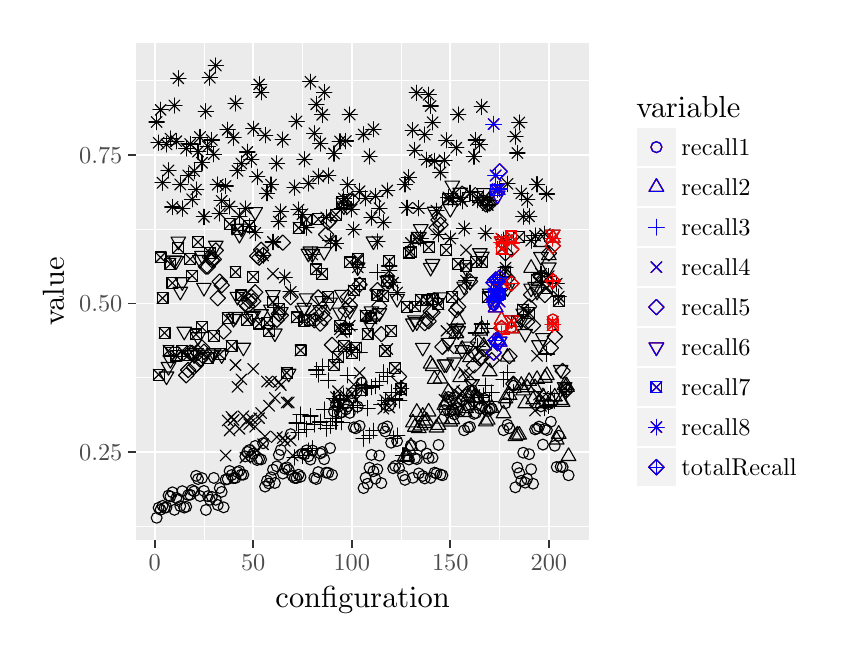
\begin{tikzpicture}[x=1pt,y=1pt]
\definecolor{fillColor}{RGB}{255,255,255}
\path[use as bounding box,fill=fillColor,fill opacity=0.00] (0,0) rectangle (289.08,216.81);
\begin{scope}
\path[clip] (  0.00,  0.00) rectangle (289.08,216.81);
\definecolor{drawColor}{RGB}{255,255,255}
\definecolor{fillColor}{RGB}{255,255,255}

\path[draw=drawColor,line width= 0.6pt,line join=round,line cap=round,fill=fillColor] (  0.00,  0.00) rectangle (289.08,216.81);
\end{scope}
\begin{scope}
\path[clip] ( 39.17, 31.53) rectangle (202.89,211.31);
\definecolor{fillColor}{gray}{0.92}

\path[fill=fillColor] ( 39.17, 31.53) rectangle (202.89,211.31);
\definecolor{drawColor}{RGB}{255,255,255}

\path[draw=drawColor,line width= 0.3pt,line join=round] ( 39.17, 36.62) --
	(202.89, 36.62);

\path[draw=drawColor,line width= 0.3pt,line join=round] ( 39.17, 90.32) --
	(202.89, 90.32);

\path[draw=drawColor,line width= 0.3pt,line join=round] ( 39.17,144.02) --
	(202.89,144.02);

\path[draw=drawColor,line width= 0.3pt,line join=round] ( 39.17,197.71) --
	(202.89,197.71);

\path[draw=drawColor,line width= 0.3pt,line join=round] ( 63.70, 31.53) --
	( 63.70,211.31);

\path[draw=drawColor,line width= 0.3pt,line join=round] ( 99.31, 31.53) --
	( 99.31,211.31);

\path[draw=drawColor,line width= 0.3pt,line join=round] (134.91, 31.53) --
	(134.91,211.31);

\path[draw=drawColor,line width= 0.3pt,line join=round] (170.52, 31.53) --
	(170.52,211.31);

\path[draw=drawColor,line width= 0.6pt,line join=round] ( 39.17, 63.47) --
	(202.89, 63.47);

\path[draw=drawColor,line width= 0.6pt,line join=round] ( 39.17,117.17) --
	(202.89,117.17);

\path[draw=drawColor,line width= 0.6pt,line join=round] ( 39.17,170.87) --
	(202.89,170.87);

\path[draw=drawColor,line width= 0.6pt,line join=round] ( 45.90, 31.53) --
	( 45.90,211.31);

\path[draw=drawColor,line width= 0.6pt,line join=round] ( 81.50, 31.53) --
	( 81.50,211.31);

\path[draw=drawColor,line width= 0.6pt,line join=round] (117.11, 31.53) --
	(117.11,211.31);

\path[draw=drawColor,line width= 0.6pt,line join=round] (152.72, 31.53) --
	(152.72,211.31);

\path[draw=drawColor,line width= 0.6pt,line join=round] (188.33, 31.53) --
	(188.33,211.31);
\definecolor{drawColor}{RGB}{0,0,0}

\path[draw=drawColor,line width= 0.4pt,line join=round,line cap=round] ( 46.61, 39.70) circle (  1.96);

\path[draw=drawColor,line width= 0.4pt,line join=round,line cap=round] ( 47.32, 43.33) circle (  1.96);

\path[draw=drawColor,line width= 0.4pt,line join=round,line cap=round] ( 48.03, 42.62) circle (  1.96);

\path[draw=drawColor,line width= 0.4pt,line join=round,line cap=round] ( 48.75, 44.02) circle (  1.96);

\path[draw=drawColor,line width= 0.4pt,line join=round,line cap=round] ( 49.46, 43.33) circle (  1.96);

\path[draw=drawColor,line width= 0.4pt,line join=round,line cap=round] ( 50.17, 43.47) circle (  1.96);

\path[draw=drawColor,line width= 0.4pt,line join=round,line cap=round] ( 50.88, 47.75) circle (  1.96);

\path[draw=drawColor,line width= 0.4pt,line join=round,line cap=round] ( 51.59, 47.40) circle (  1.96);

\path[draw=drawColor,line width= 0.4pt,line join=round,line cap=round] ( 52.31, 48.91) circle (  1.96);

\path[draw=drawColor,line width= 0.4pt,line join=round,line cap=round] ( 53.02, 42.58) circle (  1.96);

\path[draw=drawColor,line width= 0.4pt,line join=round,line cap=round] ( 53.73, 46.85) circle (  1.96);

\path[draw=drawColor,line width= 0.4pt,line join=round,line cap=round] ( 54.44, 46.45) circle (  1.96);

\path[draw=drawColor,line width= 0.4pt,line join=round,line cap=round] ( 55.15, 43.93) circle (  1.96);

\path[draw=drawColor,line width= 0.4pt,line join=round,line cap=round] ( 55.87, 49.33) circle (  1.96);

\path[draw=drawColor,line width= 0.4pt,line join=round,line cap=round] ( 56.58, 43.38) circle (  1.96);

\path[draw=drawColor,line width= 0.4pt,line join=round,line cap=round] ( 57.29, 43.69) circle (  1.96);

\path[draw=drawColor,line width= 0.4pt,line join=round,line cap=round] ( 58.00, 47.94) circle (  1.96);

\path[draw=drawColor,line width= 0.4pt,line join=round,line cap=round] ( 58.72, 48.02) circle (  1.96);

\path[draw=drawColor,line width= 0.4pt,line join=round,line cap=round] ( 59.43, 49.73) circle (  1.96);

\path[draw=drawColor,line width= 0.4pt,line join=round,line cap=round] ( 60.14, 49.26) circle (  1.96);

\path[draw=drawColor,line width= 0.4pt,line join=round,line cap=round] ( 60.85, 54.87) circle (  1.96);

\path[draw=drawColor,line width= 0.4pt,line join=round,line cap=round] ( 61.56, 53.71) circle (  1.96);

\path[draw=drawColor,line width= 0.4pt,line join=round,line cap=round] ( 62.28, 47.54) circle (  1.96);

\path[draw=drawColor,line width= 0.4pt,line join=round,line cap=round] ( 62.99, 54.04) circle (  1.96);

\path[draw=drawColor,line width= 0.4pt,line join=round,line cap=round] ( 63.70, 49.42) circle (  1.96);

\path[draw=drawColor,line width= 0.4pt,line join=round,line cap=round] ( 64.41, 42.54) circle (  1.96);

\path[draw=drawColor,line width= 0.4pt,line join=round,line cap=round] ( 65.12, 47.52) circle (  1.96);

\path[draw=drawColor,line width= 0.4pt,line join=round,line cap=round] ( 65.84, 46.21) circle (  1.96);

\path[draw=drawColor,line width= 0.4pt,line join=round,line cap=round] ( 66.55, 47.28) circle (  1.96);

\path[draw=drawColor,line width= 0.4pt,line join=round,line cap=round] ( 67.26, 54.11) circle (  1.96);

\path[draw=drawColor,line width= 0.4pt,line join=round,line cap=round] ( 67.97, 46.20) circle (  1.96);

\path[draw=drawColor,line width= 0.4pt,line join=round,line cap=round] ( 68.69, 44.33) circle (  1.96);

\path[draw=drawColor,line width= 0.4pt,line join=round,line cap=round] ( 69.40, 50.45) circle (  1.96);

\path[draw=drawColor,line width= 0.4pt,line join=round,line cap=round] ( 70.11, 49.08) circle (  1.96);

\path[draw=drawColor,line width= 0.4pt,line join=round,line cap=round] ( 70.82, 43.49) circle (  1.96);

\path[draw=drawColor,line width= 0.4pt,line join=round,line cap=round] ( 71.53, 53.52) circle (  1.96);

\path[draw=drawColor,line width= 0.4pt,line join=round,line cap=round] ( 72.25, 53.67) circle (  1.96);

\path[draw=drawColor,line width= 0.4pt,line join=round,line cap=round] ( 72.96, 56.61) circle (  1.96);

\path[draw=drawColor,line width= 0.4pt,line join=round,line cap=round] ( 73.67, 55.13) circle (  1.96);

\path[draw=drawColor,line width= 0.4pt,line join=round,line cap=round] ( 74.38, 54.06) circle (  1.96);

\path[draw=drawColor,line width= 0.4pt,line join=round,line cap=round] ( 75.09, 54.09) circle (  1.96);

\path[draw=drawColor,line width= 0.4pt,line join=round,line cap=round] ( 75.81, 56.24) circle (  1.96);

\path[draw=drawColor,line width= 0.4pt,line join=round,line cap=round] ( 76.52, 56.62) circle (  1.96);

\path[draw=drawColor,line width= 0.4pt,line join=round,line cap=round] ( 77.23, 55.28) circle (  1.96);

\path[draw=drawColor,line width= 0.4pt,line join=round,line cap=round] ( 77.94, 55.28) circle (  1.96);

\path[draw=drawColor,line width= 0.4pt,line join=round,line cap=round] ( 78.66, 61.88) circle (  1.96);

\path[draw=drawColor,line width= 0.4pt,line join=round,line cap=round] ( 79.37, 63.51) circle (  1.96);

\path[draw=drawColor,line width= 0.4pt,line join=round,line cap=round] ( 80.08, 64.18) circle (  1.96);

\path[draw=drawColor,line width= 0.4pt,line join=round,line cap=round] ( 80.79, 61.89) circle (  1.96);

\path[draw=drawColor,line width= 0.4pt,line join=round,line cap=round] ( 81.50, 62.85) circle (  1.96);

\path[draw=drawColor,line width= 0.4pt,line join=round,line cap=round] ( 82.22, 65.67) circle (  1.96);

\path[draw=drawColor,line width= 0.4pt,line join=round,line cap=round] ( 82.93, 60.58) circle (  1.96);

\path[draw=drawColor,line width= 0.4pt,line join=round,line cap=round] ( 83.64, 60.91) circle (  1.96);

\path[draw=drawColor,line width= 0.4pt,line join=round,line cap=round] ( 84.35, 60.79) circle (  1.96);

\path[draw=drawColor,line width= 0.4pt,line join=round,line cap=round] ( 85.06, 66.65) circle (  1.96);

\path[draw=drawColor,line width= 0.4pt,line join=round,line cap=round] ( 85.78, 50.98) circle (  1.96);

\path[draw=drawColor,line width= 0.4pt,line join=round,line cap=round] ( 86.49, 53.11) circle (  1.96);

\path[draw=drawColor,line width= 0.4pt,line join=round,line cap=round] ( 87.20, 52.08) circle (  1.96);

\path[draw=drawColor,line width= 0.4pt,line join=round,line cap=round] ( 87.91, 54.35) circle (  1.96);

\path[draw=drawColor,line width= 0.4pt,line join=round,line cap=round] ( 88.63, 57.10) circle (  1.96);

\path[draw=drawColor,line width= 0.4pt,line join=round,line cap=round] ( 89.34, 52.29) circle (  1.96);

\path[draw=drawColor,line width= 0.4pt,line join=round,line cap=round] ( 90.05, 58.30) circle (  1.96);

\path[draw=drawColor,line width= 0.4pt,line join=round,line cap=round] ( 90.76, 62.45) circle (  1.96);

\path[draw=drawColor,line width= 0.4pt,line join=round,line cap=round] ( 91.47, 64.22) circle (  1.96);

\path[draw=drawColor,line width= 0.4pt,line join=round,line cap=round] ( 92.19, 55.68) circle (  1.96);

\path[draw=drawColor,line width= 0.4pt,line join=round,line cap=round] ( 92.90, 57.48) circle (  1.96);

\path[draw=drawColor,line width= 0.4pt,line join=round,line cap=round] ( 93.61, 57.94) circle (  1.96);

\path[draw=drawColor,line width= 0.4pt,line join=round,line cap=round] ( 94.32, 57.05) circle (  1.96);

\path[draw=drawColor,line width= 0.4pt,line join=round,line cap=round] ( 95.03, 69.93) circle (  1.96);

\path[draw=drawColor,line width= 0.4pt,line join=round,line cap=round] ( 95.75, 54.79) circle (  1.96);

\path[draw=drawColor,line width= 0.4pt,line join=round,line cap=round] ( 96.46, 54.09) circle (  1.96);

\path[draw=drawColor,line width= 0.4pt,line join=round,line cap=round] ( 97.17, 54.08) circle (  1.96);

\path[draw=drawColor,line width= 0.4pt,line join=round,line cap=round] ( 97.88, 55.28) circle (  1.96);

\path[draw=drawColor,line width= 0.4pt,line join=round,line cap=round] ( 98.60, 54.52) circle (  1.96);

\path[draw=drawColor,line width= 0.4pt,line join=round,line cap=round] ( 99.31, 62.89) circle (  1.96);

\path[draw=drawColor,line width= 0.4pt,line join=round,line cap=round] (100.02, 62.61) circle (  1.96);

\path[draw=drawColor,line width= 0.4pt,line join=round,line cap=round] (100.73, 64.05) circle (  1.96);

\path[draw=drawColor,line width= 0.4pt,line join=round,line cap=round] (101.44, 61.90) circle (  1.96);

\path[draw=drawColor,line width= 0.4pt,line join=round,line cap=round] (102.16, 60.74) circle (  1.96);

\path[draw=drawColor,line width= 0.4pt,line join=round,line cap=round] (102.87, 64.03) circle (  1.96);

\path[draw=drawColor,line width= 0.4pt,line join=round,line cap=round] (103.58, 54.10) circle (  1.96);

\path[draw=drawColor,line width= 0.4pt,line join=round,line cap=round] (104.29, 53.70) circle (  1.96);

\path[draw=drawColor,line width= 0.4pt,line join=round,line cap=round] (105.00, 56.23) circle (  1.96);

\path[draw=drawColor,line width= 0.4pt,line join=round,line cap=round] (105.72, 62.95) circle (  1.96);

\path[draw=drawColor,line width= 0.4pt,line join=round,line cap=round] (106.43, 63.50) circle (  1.96);

\path[draw=drawColor,line width= 0.4pt,line join=round,line cap=round] (107.14, 60.87) circle (  1.96);

\path[draw=drawColor,line width= 0.4pt,line join=round,line cap=round] (107.85, 56.01) circle (  1.96);

\path[draw=drawColor,line width= 0.4pt,line join=round,line cap=round] (108.57, 55.97) circle (  1.96);

\path[draw=drawColor,line width= 0.4pt,line join=round,line cap=round] (109.28, 64.87) circle (  1.96);

\path[draw=drawColor,line width= 0.4pt,line join=round,line cap=round] (109.99, 55.25) circle (  1.96);

\path[draw=drawColor,line width= 0.4pt,line join=round,line cap=round] (110.70, 78.13) circle (  1.96);

\path[draw=drawColor,line width= 0.4pt,line join=round,line cap=round] (111.41, 80.49) circle (  1.96);

\path[draw=drawColor,line width= 0.4pt,line join=round,line cap=round] (112.13, 79.78) circle (  1.96);

\path[draw=drawColor,line width= 0.4pt,line join=round,line cap=round] (112.84, 77.58) circle (  1.96);

\path[draw=drawColor,line width= 0.4pt,line join=round,line cap=round] (113.55, 77.84) circle (  1.96);

\path[draw=drawColor,line width= 0.4pt,line join=round,line cap=round] (114.26, 81.07) circle (  1.96);

\path[draw=drawColor,line width= 0.4pt,line join=round,line cap=round] (114.97, 78.85) circle (  1.96);

\path[draw=drawColor,line width= 0.4pt,line join=round,line cap=round] (115.69, 79.96) circle (  1.96);

\path[draw=drawColor,line width= 0.4pt,line join=round,line cap=round] (116.40, 77.61) circle (  1.96);

\path[draw=drawColor,line width= 0.4pt,line join=round,line cap=round] (117.11, 84.73) circle (  1.96);

\path[draw=drawColor,line width= 0.4pt,line join=round,line cap=round] (117.82, 72.38) circle (  1.96);

\path[draw=drawColor,line width= 0.4pt,line join=round,line cap=round] (118.54, 72.04) circle (  1.96);

\path[draw=drawColor,line width= 0.4pt,line join=round,line cap=round] (119.25, 79.89) circle (  1.96);

\path[draw=drawColor,line width= 0.4pt,line join=round,line cap=round] (119.96, 72.92) circle (  1.96);

\path[draw=drawColor,line width= 0.4pt,line join=round,line cap=round] (120.67, 88.50) circle (  1.96);

\path[draw=drawColor,line width= 0.4pt,line join=round,line cap=round] (121.38, 50.44) circle (  1.96);

\path[draw=drawColor,line width= 0.4pt,line join=round,line cap=round] (122.10, 54.17) circle (  1.96);

\path[draw=drawColor,line width= 0.4pt,line join=round,line cap=round] (122.81, 52.01) circle (  1.96);

\path[draw=drawColor,line width= 0.4pt,line join=round,line cap=round] (123.52, 57.82) circle (  1.96);

\path[draw=drawColor,line width= 0.4pt,line join=round,line cap=round] (124.23, 62.44) circle (  1.96);

\path[draw=drawColor,line width= 0.4pt,line join=round,line cap=round] (124.94, 56.54) circle (  1.96);

\path[draw=drawColor,line width= 0.4pt,line join=round,line cap=round] (125.66, 53.83) circle (  1.96);

\path[draw=drawColor,line width= 0.4pt,line join=round,line cap=round] (126.37, 57.22) circle (  1.96);

\path[draw=drawColor,line width= 0.4pt,line join=round,line cap=round] (127.08, 62.17) circle (  1.96);

\path[draw=drawColor,line width= 0.4pt,line join=round,line cap=round] (127.79, 52.25) circle (  1.96);

\path[draw=drawColor,line width= 0.4pt,line join=round,line cap=round] (128.51, 72.08) circle (  1.96);

\path[draw=drawColor,line width= 0.4pt,line join=round,line cap=round] (129.22, 70.88) circle (  1.96);

\path[draw=drawColor,line width= 0.4pt,line join=round,line cap=round] (129.93, 72.72) circle (  1.96);

\path[draw=drawColor,line width= 0.4pt,line join=round,line cap=round] (130.64, 80.21) circle (  1.96);

\path[draw=drawColor,line width= 0.4pt,line join=round,line cap=round] (131.35, 66.83) circle (  1.96);

\path[draw=drawColor,line width= 0.4pt,line join=round,line cap=round] (132.07, 57.60) circle (  1.96);

\path[draw=drawColor,line width= 0.4pt,line join=round,line cap=round] (132.78, 58.42) circle (  1.96);

\path[draw=drawColor,line width= 0.4pt,line join=round,line cap=round] (133.49, 67.43) circle (  1.96);

\path[draw=drawColor,line width= 0.4pt,line join=round,line cap=round] (134.20, 57.62) circle (  1.96);

\path[draw=drawColor,line width= 0.4pt,line join=round,line cap=round] (134.91, 86.83) circle (  1.96);

\path[draw=drawColor,line width= 0.4pt,line join=round,line cap=round] (135.63, 55.03) circle (  1.96);

\path[draw=drawColor,line width= 0.4pt,line join=round,line cap=round] (136.34, 53.42) circle (  1.96);

\path[draw=drawColor,line width= 0.4pt,line join=round,line cap=round] (137.05, 62.06) circle (  1.96);

\path[draw=drawColor,line width= 0.4pt,line join=round,line cap=round] (137.76, 60.75) circle (  1.96);

\path[draw=drawColor,line width= 0.4pt,line join=round,line cap=round] (138.48, 65.89) circle (  1.96);

\path[draw=drawColor,line width= 0.4pt,line join=round,line cap=round] (139.19, 54.16) circle (  1.96);

\path[draw=drawColor,line width= 0.4pt,line join=round,line cap=round] (139.90, 61.24) circle (  1.96);

\path[draw=drawColor,line width= 0.4pt,line join=round,line cap=round] (140.61, 60.91) circle (  1.96);

\path[draw=drawColor,line width= 0.4pt,line join=round,line cap=round] (141.32, 55.74) circle (  1.96);

\path[draw=drawColor,line width= 0.4pt,line join=round,line cap=round] (142.04, 65.70) circle (  1.96);

\path[draw=drawColor,line width= 0.4pt,line join=round,line cap=round] (142.75, 54.81) circle (  1.96);

\path[draw=drawColor,line width= 0.4pt,line join=round,line cap=round] (143.46, 53.93) circle (  1.96);

\path[draw=drawColor,line width= 0.4pt,line join=round,line cap=round] (144.17, 62.92) circle (  1.96);

\path[draw=drawColor,line width= 0.4pt,line join=round,line cap=round] (144.88, 61.27) circle (  1.96);

\path[draw=drawColor,line width= 0.4pt,line join=round,line cap=round] (145.60, 54.12) circle (  1.96);

\path[draw=drawColor,line width= 0.4pt,line join=round,line cap=round] (146.31, 61.39) circle (  1.96);

\path[draw=drawColor,line width= 0.4pt,line join=round,line cap=round] (147.02, 56.02) circle (  1.96);

\path[draw=drawColor,line width= 0.4pt,line join=round,line cap=round] (147.73, 55.74) circle (  1.96);

\path[draw=drawColor,line width= 0.4pt,line join=round,line cap=round] (148.45, 66.03) circle (  1.96);

\path[draw=drawColor,line width= 0.4pt,line join=round,line cap=round] (149.16, 55.34) circle (  1.96);

\path[draw=drawColor,line width= 0.4pt,line join=round,line cap=round] (149.87, 55.06) circle (  1.96);

\path[draw=drawColor,line width= 0.4pt,line join=round,line cap=round] (150.58, 78.64) circle (  1.96);

\path[draw=drawColor,line width= 0.4pt,line join=round,line cap=round] (151.29, 80.83) circle (  1.96);

\path[draw=drawColor,line width= 0.4pt,line join=round,line cap=round] (152.01, 83.32) circle (  1.96);

\path[draw=drawColor,line width= 0.4pt,line join=round,line cap=round] (152.72, 78.16) circle (  1.96);

\path[draw=drawColor,line width= 0.4pt,line join=round,line cap=round] (153.43, 78.78) circle (  1.96);

\path[draw=drawColor,line width= 0.4pt,line join=round,line cap=round] (154.14, 77.12) circle (  1.96);

\path[draw=drawColor,line width= 0.4pt,line join=round,line cap=round] (154.85, 81.25) circle (  1.96);

\path[draw=drawColor,line width= 0.4pt,line join=round,line cap=round] (155.57, 79.42) circle (  1.96);

\path[draw=drawColor,line width= 0.4pt,line join=round,line cap=round] (156.28, 78.25) circle (  1.96);

\path[draw=drawColor,line width= 0.4pt,line join=round,line cap=round] (156.99, 82.27) circle (  1.96);

\path[draw=drawColor,line width= 0.4pt,line join=round,line cap=round] (157.70, 71.32) circle (  1.96);

\path[draw=drawColor,line width= 0.4pt,line join=round,line cap=round] (158.42, 80.32) circle (  1.96);

\path[draw=drawColor,line width= 0.4pt,line join=round,line cap=round] (159.13, 72.32) circle (  1.96);

\path[draw=drawColor,line width= 0.4pt,line join=round,line cap=round] (159.84, 72.57) circle (  1.96);

\path[draw=drawColor,line width= 0.4pt,line join=round,line cap=round] (160.55, 85.83) circle (  1.96);

\path[draw=drawColor,line width= 0.4pt,line join=round,line cap=round] (161.26, 77.26) circle (  1.96);

\path[draw=drawColor,line width= 0.4pt,line join=round,line cap=round] (161.98, 77.58) circle (  1.96);

\path[draw=drawColor,line width= 0.4pt,line join=round,line cap=round] (162.69, 83.23) circle (  1.96);

\path[draw=drawColor,line width= 0.4pt,line join=round,line cap=round] (163.40, 79.16) circle (  1.96);

\path[draw=drawColor,line width= 0.4pt,line join=round,line cap=round] (164.11, 80.08) circle (  1.96);

\path[draw=drawColor,line width= 0.4pt,line join=round,line cap=round] (164.82, 82.73) circle (  1.96);

\path[draw=drawColor,line width= 0.4pt,line join=round,line cap=round] (165.54, 78.93) circle (  1.96);

\path[draw=drawColor,line width= 0.4pt,line join=round,line cap=round] (166.25, 78.25) circle (  1.96);

\path[draw=drawColor,line width= 0.4pt,line join=round,line cap=round] (166.96, 78.97) circle (  1.96);

\path[draw=drawColor,line width= 0.4pt,line join=round,line cap=round] (167.67, 79.16) circle (  1.96);

\path[draw=drawColor,line width= 0.4pt,line join=round,line cap=round] (168.39,116.73) circle (  1.96);

\path[draw=drawColor,line width= 0.4pt,line join=round,line cap=round] (169.10,122.52) circle (  1.96);

\path[draw=drawColor,line width= 0.4pt,line join=round,line cap=round] (169.81,120.04) circle (  1.96);

\path[draw=drawColor,line width= 0.4pt,line join=round,line cap=round] (170.52,121.08) circle (  1.96);

\path[draw=drawColor,line width= 0.4pt,line join=round,line cap=round] (171.23,108.75) circle (  1.96);

\path[draw=drawColor,line width= 0.4pt,line join=round,line cap=round] (171.95, 71.37) circle (  1.96);

\path[draw=drawColor,line width= 0.4pt,line join=round,line cap=round] (172.66, 81.11) circle (  1.96);

\path[draw=drawColor,line width= 0.4pt,line join=round,line cap=round] (173.37, 73.30) circle (  1.96);

\path[draw=drawColor,line width= 0.4pt,line join=round,line cap=round] (174.08, 72.10) circle (  1.96);

\path[draw=drawColor,line width= 0.4pt,line join=round,line cap=round] (174.80,108.56) circle (  1.96);

\path[draw=drawColor,line width= 0.4pt,line join=round,line cap=round] (175.51, 87.40) circle (  1.96);

\path[draw=drawColor,line width= 0.4pt,line join=round,line cap=round] (176.22, 50.71) circle (  1.96);

\path[draw=drawColor,line width= 0.4pt,line join=round,line cap=round] (176.93, 57.86) circle (  1.96);

\path[draw=drawColor,line width= 0.4pt,line join=round,line cap=round] (177.64, 55.83) circle (  1.96);

\path[draw=drawColor,line width= 0.4pt,line join=round,line cap=round] (178.36, 53.07) circle (  1.96);

\path[draw=drawColor,line width= 0.4pt,line join=round,line cap=round] (179.07, 63.23) circle (  1.96);

\path[draw=drawColor,line width= 0.4pt,line join=round,line cap=round] (179.78, 52.40) circle (  1.96);

\path[draw=drawColor,line width= 0.4pt,line join=round,line cap=round] (180.49, 53.75) circle (  1.96);

\path[draw=drawColor,line width= 0.4pt,line join=round,line cap=round] (181.20, 62.68) circle (  1.96);

\path[draw=drawColor,line width= 0.4pt,line join=round,line cap=round] (181.92, 57.26) circle (  1.96);

\path[draw=drawColor,line width= 0.4pt,line join=round,line cap=round] (182.63, 52.01) circle (  1.96);

\path[draw=drawColor,line width= 0.4pt,line join=round,line cap=round] (183.34, 71.66) circle (  1.96);

\path[draw=drawColor,line width= 0.4pt,line join=round,line cap=round] (184.05, 71.91) circle (  1.96);

\path[draw=drawColor,line width= 0.4pt,line join=round,line cap=round] (184.77, 72.64) circle (  1.96);

\path[draw=drawColor,line width= 0.4pt,line join=round,line cap=round] (185.48, 79.98) circle (  1.96);

\path[draw=drawColor,line width= 0.4pt,line join=round,line cap=round] (186.19, 66.16) circle (  1.96);

\path[draw=drawColor,line width= 0.4pt,line join=round,line cap=round] (186.90, 71.81) circle (  1.96);

\path[draw=drawColor,line width= 0.4pt,line join=round,line cap=round] (187.61, 71.42) circle (  1.96);

\path[draw=drawColor,line width= 0.4pt,line join=round,line cap=round] (188.33, 80.79) circle (  1.96);

\path[draw=drawColor,line width= 0.4pt,line join=round,line cap=round] (189.04, 74.42) circle (  1.96);

\path[draw=drawColor,line width= 0.4pt,line join=round,line cap=round] (189.75,111.33) circle (  1.96);

\path[draw=drawColor,line width= 0.4pt,line join=round,line cap=round] (190.46, 65.73) circle (  1.96);

\path[draw=drawColor,line width= 0.4pt,line join=round,line cap=round] (191.17, 58.07) circle (  1.96);

\path[draw=drawColor,line width= 0.4pt,line join=round,line cap=round] (191.89, 69.37) circle (  1.96);

\path[draw=drawColor,line width= 0.4pt,line join=round,line cap=round] (192.60, 58.19) circle (  1.96);

\path[draw=drawColor,line width= 0.4pt,line join=round,line cap=round] (193.31, 58.02) circle (  1.96);

\path[draw=drawColor,line width= 0.4pt,line join=round,line cap=round] (194.02, 86.84) circle (  1.96);

\path[draw=drawColor,line width= 0.4pt,line join=round,line cap=round] (194.74, 86.00) circle (  1.96);

\path[draw=drawColor,line width= 0.4pt,line join=round,line cap=round] (195.45, 55.06) circle (  1.96);

\path[draw=drawColor,line width= 0.4pt,line join=round,line cap=round] (136.34, 65.02) --
	(138.98, 60.44) --
	(133.70, 60.44) --
	(136.34, 65.02);

\path[draw=drawColor,line width= 0.4pt,line join=round,line cap=round] (137.05, 64.70) --
	(139.69, 60.13) --
	(134.41, 60.13) --
	(137.05, 64.70);

\path[draw=drawColor,line width= 0.4pt,line join=round,line cap=round] (137.76, 67.33) --
	(140.41, 62.76) --
	(135.12, 62.76) --
	(137.76, 67.33);

\path[draw=drawColor,line width= 0.4pt,line join=round,line cap=round] (138.48, 68.63) --
	(141.12, 64.05) --
	(135.83, 64.05) --
	(138.48, 68.63);

\path[draw=drawColor,line width= 0.4pt,line join=round,line cap=round] (139.19, 77.14) --
	(141.83, 72.57) --
	(136.55, 72.57) --
	(139.19, 77.14);

\path[draw=drawColor,line width= 0.4pt,line join=round,line cap=round] (139.90, 75.55) --
	(142.54, 70.98) --
	(137.26, 70.98) --
	(139.90, 75.55);

\path[draw=drawColor,line width= 0.4pt,line join=round,line cap=round] (140.61, 80.93) --
	(143.25, 76.36) --
	(137.97, 76.36) --
	(140.61, 80.93);

\path[draw=drawColor,line width= 0.4pt,line join=round,line cap=round] (141.32, 75.05) --
	(143.97, 70.48) --
	(138.68, 70.48) --
	(141.32, 75.05);

\path[draw=drawColor,line width= 0.4pt,line join=round,line cap=round] (142.04, 76.07) --
	(144.68, 71.49) --
	(139.39, 71.49) --
	(142.04, 76.07);

\path[draw=drawColor,line width= 0.4pt,line join=round,line cap=round] (142.75, 79.50) --
	(145.39, 74.93) --
	(140.11, 74.93) --
	(142.75, 79.50);

\path[draw=drawColor,line width= 0.4pt,line join=round,line cap=round] (143.46, 76.90) --
	(146.10, 72.33) --
	(140.82, 72.33) --
	(143.46, 76.90);

\path[draw=drawColor,line width= 0.4pt,line join=round,line cap=round] (144.17, 77.81) --
	(146.82, 73.24) --
	(141.53, 73.24) --
	(144.17, 77.81);

\path[draw=drawColor,line width= 0.4pt,line join=round,line cap=round] (144.88, 81.07) --
	(147.53, 76.49) --
	(142.24, 76.49) --
	(144.88, 81.07);

\path[draw=drawColor,line width= 0.4pt,line join=round,line cap=round] (145.60, 98.38) --
	(148.24, 93.80) --
	(142.95, 93.80) --
	(145.60, 98.38);

\path[draw=drawColor,line width= 0.4pt,line join=round,line cap=round] (146.31, 97.44) --
	(148.95, 92.86) --
	(143.67, 92.86) --
	(146.31, 97.44);

\path[draw=drawColor,line width= 0.4pt,line join=round,line cap=round] (147.02, 92.85) --
	(149.66, 88.27) --
	(144.38, 88.27) --
	(147.02, 92.85);

\path[draw=drawColor,line width= 0.4pt,line join=round,line cap=round] (147.73, 75.30) --
	(150.38, 70.72) --
	(145.09, 70.72) --
	(147.73, 75.30);

\path[draw=drawColor,line width= 0.4pt,line join=round,line cap=round] (148.45, 76.23) --
	(151.09, 71.65) --
	(145.80, 71.65) --
	(148.45, 76.23);

\path[draw=drawColor,line width= 0.4pt,line join=round,line cap=round] (149.16, 92.98) --
	(151.80, 88.40) --
	(146.52, 88.40) --
	(149.16, 92.98);

\path[draw=drawColor,line width= 0.4pt,line join=round,line cap=round] (149.87, 78.47) --
	(152.51, 73.89) --
	(147.23, 73.89) --
	(149.87, 78.47);

\path[draw=drawColor,line width= 0.4pt,line join=round,line cap=round] (150.58, 83.44) --
	(153.22, 78.86) --
	(147.94, 78.86) --
	(150.58, 83.44);

\path[draw=drawColor,line width= 0.4pt,line join=round,line cap=round] (151.29, 84.67) --
	(153.94, 80.09) --
	(148.65, 80.09) --
	(151.29, 84.67);

\path[draw=drawColor,line width= 0.4pt,line join=round,line cap=round] (152.01, 88.28) --
	(154.65, 83.70) --
	(149.36, 83.70) --
	(152.01, 88.28);

\path[draw=drawColor,line width= 0.4pt,line join=round,line cap=round] (152.72, 77.47) --
	(155.36, 72.89) --
	(150.08, 72.89) --
	(152.72, 77.47);

\path[draw=drawColor,line width= 0.4pt,line join=round,line cap=round] (153.43, 78.26) --
	(156.07, 73.69) --
	(150.79, 73.69) --
	(153.43, 78.26);

\path[draw=drawColor,line width= 0.4pt,line join=round,line cap=round] (154.14, 81.57) --
	(156.79, 77.00) --
	(151.50, 77.00) --
	(154.14, 81.57);

\path[draw=drawColor,line width= 0.4pt,line join=round,line cap=round] (154.85,109.35) --
	(157.50,104.77) --
	(152.21,104.77) --
	(154.85,109.35);

\path[draw=drawColor,line width= 0.4pt,line join=round,line cap=round] (155.57,114.33) --
	(158.21,109.76) --
	(152.92,109.76) --
	(155.57,114.33);

\path[draw=drawColor,line width= 0.4pt,line join=round,line cap=round] (156.28, 93.50) --
	(158.92, 88.93) --
	(153.64, 88.93) --
	(156.28, 93.50);

\path[draw=drawColor,line width= 0.4pt,line join=round,line cap=round] (156.99,103.73) --
	(159.63, 99.15) --
	(154.35, 99.15) --
	(156.99,103.73);

\path[draw=drawColor,line width= 0.4pt,line join=round,line cap=round] (157.70, 80.90) --
	(160.35, 76.32) --
	(155.06, 76.32) --
	(157.70, 80.90);

\path[draw=drawColor,line width= 0.4pt,line join=round,line cap=round] (158.42, 82.29) --
	(161.06, 77.71) --
	(155.77, 77.71) --
	(158.42, 82.29);

\path[draw=drawColor,line width= 0.4pt,line join=round,line cap=round] (159.13, 86.47) --
	(161.77, 81.89) --
	(156.49, 81.89) --
	(159.13, 86.47);

\path[draw=drawColor,line width= 0.4pt,line join=round,line cap=round] (159.84,100.73) --
	(162.48, 96.15) --
	(157.20, 96.15) --
	(159.84,100.73);

\path[draw=drawColor,line width= 0.4pt,line join=round,line cap=round] (160.55, 87.75) --
	(163.19, 83.18) --
	(157.91, 83.18) --
	(160.55, 87.75);

\path[draw=drawColor,line width= 0.4pt,line join=round,line cap=round] (161.26, 86.04) --
	(163.91, 81.46) --
	(158.62, 81.46) --
	(161.26, 86.04);

\path[draw=drawColor,line width= 0.4pt,line join=round,line cap=round] (161.98, 86.19) --
	(164.62, 81.61) --
	(159.33, 81.61) --
	(161.98, 86.19);

\path[draw=drawColor,line width= 0.4pt,line join=round,line cap=round] (162.69, 85.91) --
	(165.33, 81.34) --
	(160.05, 81.34) --
	(162.69, 85.91);

\path[draw=drawColor,line width= 0.4pt,line join=round,line cap=round] (163.40,110.28) --
	(166.04,105.70) --
	(160.76,105.70) --
	(163.40,110.28);

\path[draw=drawColor,line width= 0.4pt,line join=round,line cap=round] (164.11,111.12) --
	(166.76,106.55) --
	(161.47,106.55) --
	(164.11,111.12);

\path[draw=drawColor,line width= 0.4pt,line join=round,line cap=round] (164.82,104.90) --
	(167.47,100.33) --
	(162.18,100.33) --
	(164.82,104.90);

\path[draw=drawColor,line width= 0.4pt,line join=round,line cap=round] (165.54, 77.48) --
	(168.18, 72.91) --
	(162.89, 72.91) --
	(165.54, 77.48);

\path[draw=drawColor,line width= 0.4pt,line join=round,line cap=round] (166.25, 78.11) --
	(168.89, 73.53) --
	(163.61, 73.53) --
	(166.25, 78.11);

\path[draw=drawColor,line width= 0.4pt,line join=round,line cap=round] (166.96, 95.63) --
	(169.60, 91.05) --
	(164.32, 91.05) --
	(166.96, 95.63);

\path[draw=drawColor,line width= 0.4pt,line join=round,line cap=round] (167.67, 82.42) --
	(170.32, 77.85) --
	(165.03, 77.85) --
	(167.67, 82.42);

\path[draw=drawColor,line width= 0.4pt,line join=round,line cap=round] (168.39,122.08) --
	(171.03,117.51) --
	(165.74,117.51) --
	(168.39,122.08);

\path[draw=drawColor,line width= 0.4pt,line join=round,line cap=round] (169.10,118.70) --
	(171.74,114.13) --
	(166.46,114.13) --
	(169.10,118.70);

\path[draw=drawColor,line width= 0.4pt,line join=round,line cap=round] (169.81,106.95) --
	(172.45,102.38) --
	(167.17,102.38) --
	(169.81,106.95);

\path[draw=drawColor,line width= 0.4pt,line join=round,line cap=round] (170.52,106.29) --
	(173.16,101.71) --
	(167.88,101.71) --
	(170.52,106.29);

\path[draw=drawColor,line width= 0.4pt,line join=round,line cap=round] (171.23,114.29) --
	(173.88,109.71) --
	(168.59,109.71) --
	(171.23,114.29);

\path[draw=drawColor,line width= 0.4pt,line join=round,line cap=round] (171.95, 80.43) --
	(174.59, 75.85) --
	(169.30, 75.85) --
	(171.95, 80.43);

\path[draw=drawColor,line width= 0.4pt,line join=round,line cap=round] (172.66, 85.83) --
	(175.30, 81.26) --
	(170.02, 81.26) --
	(172.66, 85.83);

\path[draw=drawColor,line width= 0.4pt,line join=round,line cap=round] (173.37,100.89) --
	(176.01, 96.31) --
	(170.73, 96.31) --
	(173.37,100.89);

\path[draw=drawColor,line width= 0.4pt,line join=round,line cap=round] (174.08, 87.12) --
	(176.73, 82.54) --
	(171.44, 82.54) --
	(174.08, 87.12);

\path[draw=drawColor,line width= 0.4pt,line join=round,line cap=round] (174.80,111.07) --
	(177.44,106.50) --
	(172.15,106.50) --
	(174.80,111.07);

\path[draw=drawColor,line width= 0.4pt,line join=round,line cap=round] (175.51, 90.66) --
	(178.15, 86.09) --
	(172.86, 86.09) --
	(175.51, 90.66);

\path[draw=drawColor,line width= 0.4pt,line join=round,line cap=round] (176.22, 72.15) --
	(178.86, 67.57) --
	(173.58, 67.57) --
	(176.22, 72.15);

\path[draw=drawColor,line width= 0.4pt,line join=round,line cap=round] (176.93, 72.72) --
	(179.57, 68.14) --
	(174.29, 68.14) --
	(176.93, 72.72);

\path[draw=drawColor,line width= 0.4pt,line join=round,line cap=round] (177.64, 72.70) --
	(180.29, 68.12) --
	(175.00, 68.12) --
	(177.64, 72.70);

\path[draw=drawColor,line width= 0.4pt,line join=round,line cap=round] (178.36, 90.68) --
	(181.00, 86.10) --
	(175.71, 86.10) --
	(178.36, 90.68);

\path[draw=drawColor,line width= 0.4pt,line join=round,line cap=round] (179.07, 88.67) --
	(181.71, 84.10) --
	(176.43, 84.10) --
	(179.07, 88.67);

\path[draw=drawColor,line width= 0.4pt,line join=round,line cap=round] (179.78, 84.05) --
	(182.42, 79.47) --
	(177.14, 79.47) --
	(179.78, 84.05);

\path[draw=drawColor,line width= 0.4pt,line join=round,line cap=round] (180.49, 89.82) --
	(183.13, 85.24) --
	(177.85, 85.24) --
	(180.49, 89.82);

\path[draw=drawColor,line width= 0.4pt,line join=round,line cap=round] (181.20, 92.11) --
	(183.85, 87.53) --
	(178.56, 87.53) --
	(181.20, 92.11);

\path[draw=drawColor,line width= 0.4pt,line join=round,line cap=round] (181.92,132.99) --
	(184.56,128.41) --
	(179.27,128.41) --
	(181.92,132.99);

\path[draw=drawColor,line width= 0.4pt,line join=round,line cap=round] (182.63, 85.49) --
	(185.27, 80.91) --
	(179.99, 80.91) --
	(182.63, 85.49);

\path[draw=drawColor,line width= 0.4pt,line join=round,line cap=round] (183.34, 89.85) --
	(185.98, 85.27) --
	(180.70, 85.27) --
	(183.34, 89.85);

\path[draw=drawColor,line width= 0.4pt,line join=round,line cap=round] (184.05, 92.83) --
	(186.70, 88.25) --
	(181.41, 88.25) --
	(184.05, 92.83);

\path[draw=drawColor,line width= 0.4pt,line join=round,line cap=round] (184.77, 84.05) --
	(187.41, 79.47) --
	(182.12, 79.47) --
	(184.77, 84.05);

\path[draw=drawColor,line width= 0.4pt,line join=round,line cap=round] (185.48,142.30) --
	(188.12,137.72) --
	(182.83,137.72) --
	(185.48,142.30);

\path[draw=drawColor,line width= 0.4pt,line join=round,line cap=round] (186.19, 86.61) --
	(188.83, 82.03) --
	(183.55, 82.03) --
	(186.19, 86.61);

\path[draw=drawColor,line width= 0.4pt,line join=round,line cap=round] (186.90, 93.26) --
	(189.54, 88.68) --
	(184.26, 88.68) --
	(186.90, 93.26);

\path[draw=drawColor,line width= 0.4pt,line join=round,line cap=round] (187.61, 94.24) --
	(190.26, 89.66) --
	(184.97, 89.66) --
	(187.61, 94.24);

\path[draw=drawColor,line width= 0.4pt,line join=round,line cap=round] (188.33,137.55) --
	(190.97,132.97) --
	(185.68,132.97) --
	(188.33,137.55);

\path[draw=drawColor,line width= 0.4pt,line join=round,line cap=round] (189.04, 85.24) --
	(191.68, 80.66) --
	(186.40, 80.66) --
	(189.04, 85.24);

\path[draw=drawColor,line width= 0.4pt,line join=round,line cap=round] (189.75,143.87) --
	(192.39,139.29) --
	(187.11,139.29) --
	(189.75,143.87);

\path[draw=drawColor,line width= 0.4pt,line join=round,line cap=round] (190.46, 86.46) --
	(193.10, 81.89) --
	(187.82, 81.89) --
	(190.46, 86.46);

\path[draw=drawColor,line width= 0.4pt,line join=round,line cap=round] (191.17, 70.93) --
	(193.82, 66.35) --
	(188.53, 66.35) --
	(191.17, 70.93);

\path[draw=drawColor,line width= 0.4pt,line join=round,line cap=round] (191.89, 73.03) --
	(194.53, 68.45) --
	(189.24, 68.45) --
	(191.89, 73.03);

\path[draw=drawColor,line width= 0.4pt,line join=round,line cap=round] (192.60, 85.22) --
	(195.24, 80.65) --
	(189.96, 80.65) --
	(192.60, 85.22);

\path[draw=drawColor,line width= 0.4pt,line join=round,line cap=round] (193.31, 84.51) --
	(195.95, 79.94) --
	(190.67, 79.94) --
	(193.31, 84.51);

\path[draw=drawColor,line width= 0.4pt,line join=round,line cap=round] (194.02, 90.66) --
	(196.67, 86.08) --
	(191.38, 86.08) --
	(194.02, 90.66);

\path[draw=drawColor,line width= 0.4pt,line join=round,line cap=round] (194.74, 90.53) --
	(197.38, 85.95) --
	(192.09, 85.95) --
	(194.74, 90.53);

\path[draw=drawColor,line width= 0.4pt,line join=round,line cap=round] (195.45, 64.98) --
	(198.09, 60.40) --
	(192.80, 60.40) --
	(195.45, 64.98);

\path[draw=drawColor,line width= 0.4pt,line join=round,line cap=round] ( 93.68, 61.53) -- ( 99.23, 61.53);

\path[draw=drawColor,line width= 0.4pt,line join=round,line cap=round] ( 96.46, 58.76) -- ( 96.46, 64.31);

\path[draw=drawColor,line width= 0.4pt,line join=round,line cap=round] ( 94.40, 73.97) -- ( 99.95, 73.97);

\path[draw=drawColor,line width= 0.4pt,line join=round,line cap=round] ( 97.17, 71.19) -- ( 97.17, 76.74);

\path[draw=drawColor,line width= 0.4pt,line join=round,line cap=round] ( 95.11, 70.63) -- (100.66, 70.63);

\path[draw=drawColor,line width= 0.4pt,line join=round,line cap=round] ( 97.88, 67.86) -- ( 97.88, 73.41);

\path[draw=drawColor,line width= 0.4pt,line join=round,line cap=round] ( 95.82, 77.00) -- (101.37, 77.00);

\path[draw=drawColor,line width= 0.4pt,line join=round,line cap=round] ( 98.60, 74.23) -- ( 98.60, 79.78);

\path[draw=drawColor,line width= 0.4pt,line join=round,line cap=round] ( 96.53, 62.09) -- (102.08, 62.09);

\path[draw=drawColor,line width= 0.4pt,line join=round,line cap=round] ( 99.31, 59.31) -- ( 99.31, 64.86);

\path[draw=drawColor,line width= 0.4pt,line join=round,line cap=round] ( 97.24, 73.65) -- (102.79, 73.65);

\path[draw=drawColor,line width= 0.4pt,line join=round,line cap=round] (100.02, 70.87) -- (100.02, 76.42);

\path[draw=drawColor,line width= 0.4pt,line join=round,line cap=round] ( 97.96, 71.76) -- (103.51, 71.76);

\path[draw=drawColor,line width= 0.4pt,line join=round,line cap=round] (100.73, 68.98) -- (100.73, 74.53);

\path[draw=drawColor,line width= 0.4pt,line join=round,line cap=round] ( 98.67, 63.94) -- (104.22, 63.94);

\path[draw=drawColor,line width= 0.4pt,line join=round,line cap=round] (101.44, 61.17) -- (101.44, 66.72);

\path[draw=drawColor,line width= 0.4pt,line join=round,line cap=round] ( 99.38, 76.48) -- (104.93, 76.48);

\path[draw=drawColor,line width= 0.4pt,line join=round,line cap=round] (102.16, 73.70) -- (102.16, 79.25);

\path[draw=drawColor,line width= 0.4pt,line join=round,line cap=round] (100.09, 64.83) -- (105.64, 64.83);

\path[draw=drawColor,line width= 0.4pt,line join=round,line cap=round] (102.87, 62.06) -- (102.87, 67.61);

\path[draw=drawColor,line width= 0.4pt,line join=round,line cap=round] (100.81, 73.43) -- (106.36, 73.43);

\path[draw=drawColor,line width= 0.4pt,line join=round,line cap=round] (103.58, 70.65) -- (103.58, 76.20);

\path[draw=drawColor,line width= 0.4pt,line join=round,line cap=round] (101.52, 93.10) -- (107.07, 93.10);

\path[draw=drawColor,line width= 0.4pt,line join=round,line cap=round] (104.29, 90.33) -- (104.29, 95.88);

\path[draw=drawColor,line width= 0.4pt,line join=round,line cap=round] (102.23, 91.49) -- (107.78, 91.49);

\path[draw=drawColor,line width= 0.4pt,line join=round,line cap=round] (105.00, 88.72) -- (105.00, 94.27);

\path[draw=drawColor,line width= 0.4pt,line join=round,line cap=round] (102.94, 74.33) -- (108.49, 74.33);

\path[draw=drawColor,line width= 0.4pt,line join=round,line cap=round] (105.72, 71.56) -- (105.72, 77.11);

\path[draw=drawColor,line width= 0.4pt,line join=round,line cap=round] (103.65, 94.36) -- (109.20, 94.36);

\path[draw=drawColor,line width= 0.4pt,line join=round,line cap=round] (106.43, 91.59) -- (106.43, 97.14);

\path[draw=drawColor,line width= 0.4pt,line join=round,line cap=round] (104.37, 78.78) -- (109.92, 78.78);

\path[draw=drawColor,line width= 0.4pt,line join=round,line cap=round] (107.14, 76.01) -- (107.14, 81.56);

\path[draw=drawColor,line width= 0.4pt,line join=round,line cap=round] (105.08, 71.90) -- (110.63, 71.90);

\path[draw=drawColor,line width= 0.4pt,line join=round,line cap=round] (107.85, 69.12) -- (107.85, 74.67);

\path[draw=drawColor,line width= 0.4pt,line join=round,line cap=round] (105.79, 89.32) -- (111.34, 89.32);

\path[draw=drawColor,line width= 0.4pt,line join=round,line cap=round] (108.57, 86.55) -- (108.57, 92.10);

\path[draw=drawColor,line width= 0.4pt,line join=round,line cap=round] (106.50, 73.02) -- (112.05, 73.02);

\path[draw=drawColor,line width= 0.4pt,line join=round,line cap=round] (109.28, 70.24) -- (109.28, 75.79);

\path[draw=drawColor,line width= 0.4pt,line join=round,line cap=round] (107.21, 75.73) -- (112.76, 75.73);

\path[draw=drawColor,line width= 0.4pt,line join=round,line cap=round] (109.99, 72.96) -- (109.99, 78.51);

\path[draw=drawColor,line width= 0.4pt,line join=round,line cap=round] (107.93, 82.70) -- (113.48, 82.70);

\path[draw=drawColor,line width= 0.4pt,line join=round,line cap=round] (110.70, 79.92) -- (110.70, 85.47);

\path[draw=drawColor,line width= 0.4pt,line join=round,line cap=round] (108.64, 74.43) -- (114.19, 74.43);

\path[draw=drawColor,line width= 0.4pt,line join=round,line cap=round] (111.41, 71.66) -- (111.41, 77.21);

\path[draw=drawColor,line width= 0.4pt,line join=round,line cap=round] (109.35, 79.51) -- (114.90, 79.51);

\path[draw=drawColor,line width= 0.4pt,line join=round,line cap=round] (112.13, 76.73) -- (112.13, 82.28);

\path[draw=drawColor,line width= 0.4pt,line join=round,line cap=round] (110.06, 82.28) -- (115.61, 82.28);

\path[draw=drawColor,line width= 0.4pt,line join=round,line cap=round] (112.84, 79.50) -- (112.84, 85.05);

\path[draw=drawColor,line width= 0.4pt,line join=round,line cap=round] (110.78, 74.24) -- (116.33, 74.24);

\path[draw=drawColor,line width= 0.4pt,line join=round,line cap=round] (113.55, 71.47) -- (113.55, 77.02);

\path[draw=drawColor,line width= 0.4pt,line join=round,line cap=round] (111.49, 83.83) -- (117.04, 83.83);

\path[draw=drawColor,line width= 0.4pt,line join=round,line cap=round] (114.26, 81.06) -- (114.26, 86.61);

\path[draw=drawColor,line width= 0.4pt,line join=round,line cap=round] (112.20,109.37) -- (117.75,109.37);

\path[draw=drawColor,line width= 0.4pt,line join=round,line cap=round] (114.97,106.59) -- (114.97,112.14);

\path[draw=drawColor,line width= 0.4pt,line join=round,line cap=round] (112.91, 91.20) -- (118.46, 91.20);

\path[draw=drawColor,line width= 0.4pt,line join=round,line cap=round] (115.69, 88.43) -- (115.69, 93.98);

\path[draw=drawColor,line width= 0.4pt,line join=round,line cap=round] (113.62,107.80) -- (119.17,107.80);

\path[draw=drawColor,line width= 0.4pt,line join=round,line cap=round] (116.40,105.02) -- (116.40,110.57);

\path[draw=drawColor,line width= 0.4pt,line join=round,line cap=round] (114.34,100.61) -- (119.89,100.61);

\path[draw=drawColor,line width= 0.4pt,line join=round,line cap=round] (117.11, 97.83) -- (117.11,103.38);

\path[draw=drawColor,line width= 0.4pt,line join=round,line cap=round] (115.05, 79.41) -- (120.60, 79.41);

\path[draw=drawColor,line width= 0.4pt,line join=round,line cap=round] (117.82, 76.64) -- (117.82, 82.19);

\path[draw=drawColor,line width= 0.4pt,line join=round,line cap=round] (115.76, 83.91) -- (121.31, 83.91);

\path[draw=drawColor,line width= 0.4pt,line join=round,line cap=round] (118.54, 81.14) -- (118.54, 86.69);

\path[draw=drawColor,line width= 0.4pt,line join=round,line cap=round] (116.47, 80.27) -- (122.02, 80.27);

\path[draw=drawColor,line width= 0.4pt,line join=round,line cap=round] (119.25, 77.50) -- (119.25, 83.05);

\path[draw=drawColor,line width= 0.4pt,line join=round,line cap=round] (117.18, 99.31) -- (122.73, 99.31);

\path[draw=drawColor,line width= 0.4pt,line join=round,line cap=round] (119.96, 96.54) -- (119.96,102.09);

\path[draw=drawColor,line width= 0.4pt,line join=round,line cap=round] (117.90, 87.39) -- (123.45, 87.39);

\path[draw=drawColor,line width= 0.4pt,line join=round,line cap=round] (120.67, 84.61) -- (120.67, 90.16);

\path[draw=drawColor,line width= 0.4pt,line join=round,line cap=round] (118.61, 68.25) -- (124.16, 68.25);

\path[draw=drawColor,line width= 0.4pt,line join=round,line cap=round] (121.38, 65.48) -- (121.38, 71.03);

\path[draw=drawColor,line width= 0.4pt,line join=round,line cap=round] (119.32, 86.41) -- (124.87, 86.41);

\path[draw=drawColor,line width= 0.4pt,line join=round,line cap=round] (122.10, 83.64) -- (122.10, 89.19);

\path[draw=drawColor,line width= 0.4pt,line join=round,line cap=round] (120.03, 79.34) -- (125.58, 79.34);

\path[draw=drawColor,line width= 0.4pt,line join=round,line cap=round] (122.81, 76.56) -- (122.81, 82.11);

\path[draw=drawColor,line width= 0.4pt,line join=round,line cap=round] (120.75, 69.43) -- (126.30, 69.43);

\path[draw=drawColor,line width= 0.4pt,line join=round,line cap=round] (123.52, 66.66) -- (123.52, 72.21);

\path[draw=drawColor,line width= 0.4pt,line join=round,line cap=round] (121.46, 86.95) -- (127.01, 86.95);

\path[draw=drawColor,line width= 0.4pt,line join=round,line cap=round] (124.23, 84.18) -- (124.23, 89.73);

\path[draw=drawColor,line width= 0.4pt,line join=round,line cap=round] (122.17, 71.15) -- (127.72, 71.15);

\path[draw=drawColor,line width= 0.4pt,line join=round,line cap=round] (124.94, 68.37) -- (124.94, 73.92);

\path[draw=drawColor,line width= 0.4pt,line join=round,line cap=round] (122.88, 87.39) -- (128.43, 87.39);

\path[draw=drawColor,line width= 0.4pt,line join=round,line cap=round] (125.66, 84.62) -- (125.66, 90.17);

\path[draw=drawColor,line width= 0.4pt,line join=round,line cap=round] (123.59,128.45) -- (129.14,128.45);

\path[draw=drawColor,line width= 0.4pt,line join=round,line cap=round] (126.37,125.68) -- (126.37,131.23);

\path[draw=drawColor,line width= 0.4pt,line join=round,line cap=round] (124.31, 88.86) -- (129.86, 88.86);

\path[draw=drawColor,line width= 0.4pt,line join=round,line cap=round] (127.08, 86.09) -- (127.08, 91.64);

\path[draw=drawColor,line width= 0.4pt,line join=round,line cap=round] (125.02, 80.80) -- (130.57, 80.80);

\path[draw=drawColor,line width= 0.4pt,line join=round,line cap=round] (127.79, 78.03) -- (127.79, 83.58);

\path[draw=drawColor,line width= 0.4pt,line join=round,line cap=round] (125.73, 92.25) -- (131.28, 92.25);

\path[draw=drawColor,line width= 0.4pt,line join=round,line cap=round] (128.51, 89.48) -- (128.51, 95.03);

\path[draw=drawColor,line width= 0.4pt,line join=round,line cap=round] (126.44, 81.95) -- (131.99, 81.95);

\path[draw=drawColor,line width= 0.4pt,line join=round,line cap=round] (129.22, 79.18) -- (129.22, 84.73);

\path[draw=drawColor,line width= 0.4pt,line join=round,line cap=round] (127.15, 90.90) -- (132.70, 90.90);

\path[draw=drawColor,line width= 0.4pt,line join=round,line cap=round] (129.93, 88.12) -- (129.93, 93.67);

\path[draw=drawColor,line width= 0.4pt,line join=round,line cap=round] (127.87,130.67) -- (133.42,130.67);

\path[draw=drawColor,line width= 0.4pt,line join=round,line cap=round] (130.64,127.89) -- (130.64,133.44);

\path[draw=drawColor,line width= 0.4pt,line join=round,line cap=round] (128.58, 85.01) -- (134.13, 85.01);

\path[draw=drawColor,line width= 0.4pt,line join=round,line cap=round] (131.35, 82.24) -- (131.35, 87.79);

\path[draw=drawColor,line width= 0.4pt,line join=round,line cap=round] (129.29, 68.31) -- (134.84, 68.31);

\path[draw=drawColor,line width= 0.4pt,line join=round,line cap=round] (132.07, 65.54) -- (132.07, 71.09);

\path[draw=drawColor,line width= 0.4pt,line join=round,line cap=round] (130.00, 82.62) -- (135.55, 82.62);

\path[draw=drawColor,line width= 0.4pt,line join=round,line cap=round] (132.78, 79.85) -- (132.78, 85.40);

\path[draw=drawColor,line width= 0.4pt,line join=round,line cap=round] (130.72, 69.40) -- (136.27, 69.40);

\path[draw=drawColor,line width= 0.4pt,line join=round,line cap=round] (133.49, 66.62) -- (133.49, 72.17);

\path[draw=drawColor,line width= 0.4pt,line join=round,line cap=round] (131.43, 82.13) -- (136.98, 82.13);

\path[draw=drawColor,line width= 0.4pt,line join=round,line cap=round] (134.20, 79.36) -- (134.20, 84.91);

\path[draw=drawColor,line width= 0.4pt,line join=round,line cap=round] (132.14, 86.58) -- (137.69, 86.58);

\path[draw=drawColor,line width= 0.4pt,line join=round,line cap=round] (134.91, 83.81) -- (134.91, 89.36);

\path[draw=drawColor,line width= 0.4pt,line join=round,line cap=round] (132.85, 62.30) -- (138.40, 62.30);

\path[draw=drawColor,line width= 0.4pt,line join=round,line cap=round] (135.63, 59.53) -- (135.63, 65.08);

\path[draw=drawColor,line width= 0.4pt,line join=round,line cap=round] (158.49, 81.37) -- (164.04, 81.37);

\path[draw=drawColor,line width= 0.4pt,line join=round,line cap=round] (161.26, 78.60) -- (161.26, 84.15);

\path[draw=drawColor,line width= 0.4pt,line join=round,line cap=round] (159.20,106.46) -- (164.75,106.46);

\path[draw=drawColor,line width= 0.4pt,line join=round,line cap=round] (161.98,103.69) -- (161.98,109.24);

\path[draw=drawColor,line width= 0.4pt,line join=round,line cap=round] (159.91,101.71) -- (165.46,101.71);

\path[draw=drawColor,line width= 0.4pt,line join=round,line cap=round] (162.69, 98.94) -- (162.69,104.49);

\path[draw=drawColor,line width= 0.4pt,line join=round,line cap=round] (160.63, 83.24) -- (166.18, 83.24);

\path[draw=drawColor,line width= 0.4pt,line join=round,line cap=round] (163.40, 80.46) -- (163.40, 86.01);

\path[draw=drawColor,line width= 0.4pt,line join=round,line cap=round] (161.34,109.74) -- (166.89,109.74);

\path[draw=drawColor,line width= 0.4pt,line join=round,line cap=round] (164.11,106.97) -- (164.11,112.52);

\path[draw=drawColor,line width= 0.4pt,line join=round,line cap=round] (162.05, 83.88) -- (167.60, 83.88);

\path[draw=drawColor,line width= 0.4pt,line join=round,line cap=round] (164.82, 81.11) -- (164.82, 86.66);

\path[draw=drawColor,line width= 0.4pt,line join=round,line cap=round] (162.76, 87.46) -- (168.31, 87.46);

\path[draw=drawColor,line width= 0.4pt,line join=round,line cap=round] (165.54, 84.68) -- (165.54, 90.23);

\path[draw=drawColor,line width= 0.4pt,line join=round,line cap=round] (163.47,108.20) -- (169.02,108.20);

\path[draw=drawColor,line width= 0.4pt,line join=round,line cap=round] (166.25,105.43) -- (166.25,110.98);

\path[draw=drawColor,line width= 0.4pt,line join=round,line cap=round] (164.19, 81.83) -- (169.74, 81.83);

\path[draw=drawColor,line width= 0.4pt,line join=round,line cap=round] (166.96, 79.06) -- (166.96, 84.61);

\path[draw=drawColor,line width= 0.4pt,line join=round,line cap=round] (164.90, 84.94) -- (170.45, 84.94);

\path[draw=drawColor,line width= 0.4pt,line join=round,line cap=round] (167.67, 82.17) -- (167.67, 87.72);

\path[draw=drawColor,line width= 0.4pt,line join=round,line cap=round] (165.61,122.06) -- (171.16,122.06);

\path[draw=drawColor,line width= 0.4pt,line join=round,line cap=round] (168.39,119.28) -- (168.39,124.83);

\path[draw=drawColor,line width= 0.4pt,line join=round,line cap=round] (166.32,103.85) -- (171.87,103.85);

\path[draw=drawColor,line width= 0.4pt,line join=round,line cap=round] (169.10,101.08) -- (169.10,106.63);

\path[draw=drawColor,line width= 0.4pt,line join=round,line cap=round] (167.04,119.98) -- (172.58,119.98);

\path[draw=drawColor,line width= 0.4pt,line join=round,line cap=round] (169.81,117.20) -- (169.81,122.75);

\path[draw=drawColor,line width= 0.4pt,line join=round,line cap=round] (167.75,122.53) -- (173.30,122.53);

\path[draw=drawColor,line width= 0.4pt,line join=round,line cap=round] (170.52,119.75) -- (170.52,125.30);

\path[draw=drawColor,line width= 0.4pt,line join=round,line cap=round] (168.46,106.13) -- (174.01,106.13);

\path[draw=drawColor,line width= 0.4pt,line join=round,line cap=round] (171.23,103.36) -- (171.23,108.91);

\path[draw=drawColor,line width= 0.4pt,line join=round,line cap=round] (169.17, 89.80) -- (174.72, 89.80);

\path[draw=drawColor,line width= 0.4pt,line join=round,line cap=round] (171.95, 87.03) -- (171.95, 92.58);

\path[draw=drawColor,line width= 0.4pt,line join=round,line cap=round] (169.88,134.93) -- (175.43,134.93);

\path[draw=drawColor,line width= 0.4pt,line join=round,line cap=round] (172.66,132.16) -- (172.66,137.71);

\path[draw=drawColor,line width= 0.4pt,line join=round,line cap=round] (170.60, 92.16) -- (176.15, 92.16);

\path[draw=drawColor,line width= 0.4pt,line join=round,line cap=round] (173.37, 89.38) -- (173.37, 94.93);

\path[draw=drawColor,line width= 0.4pt,line join=round,line cap=round] (171.31, 82.56) -- (176.86, 82.56);

\path[draw=drawColor,line width= 0.4pt,line join=round,line cap=round] (174.08, 79.78) -- (174.08, 85.33);

\path[draw=drawColor,line width= 0.4pt,line join=round,line cap=round] (172.02,139.00) -- (177.57,139.00);

\path[draw=drawColor,line width= 0.4pt,line join=round,line cap=round] (174.80,136.23) -- (174.80,141.78);

\path[draw=drawColor,line width= 0.4pt,line join=round,line cap=round] (172.73, 85.01) -- (178.28, 85.01);

\path[draw=drawColor,line width= 0.4pt,line join=round,line cap=round] (175.51, 82.23) -- (175.51, 87.78);

\path[draw=drawColor,line width= 0.4pt,line join=round,line cap=round] (184.13, 79.42) -- (189.68, 79.42);

\path[draw=drawColor,line width= 0.4pt,line join=round,line cap=round] (186.90, 76.65) -- (186.90, 82.20);

\path[draw=drawColor,line width= 0.4pt,line join=round,line cap=round] (184.84, 98.90) -- (190.39, 98.90);

\path[draw=drawColor,line width= 0.4pt,line join=round,line cap=round] (187.61, 96.12) -- (187.61,101.67);

\path[draw=drawColor,line width= 0.4pt,line join=round,line cap=round] (185.55, 80.11) -- (191.10, 80.11);

\path[draw=drawColor,line width= 0.4pt,line join=round,line cap=round] (188.33, 77.33) -- (188.33, 82.88);

\path[draw=drawColor,line width= 0.4pt,line join=round,line cap=round] (186.26, 84.64) -- (191.81, 84.64);

\path[draw=drawColor,line width= 0.4pt,line join=round,line cap=round] (189.04, 81.87) -- (189.04, 87.42);

\path[draw=drawColor,line width= 0.4pt,line join=round,line cap=round] (186.98,109.46) -- (192.52,109.46);

\path[draw=drawColor,line width= 0.4pt,line join=round,line cap=round] (189.75,106.68) -- (189.75,112.23);

\path[draw=drawColor,line width= 0.4pt,line join=round,line cap=round] (187.69, 82.02) -- (193.24, 82.02);

\path[draw=drawColor,line width= 0.4pt,line join=round,line cap=round] (190.46, 79.24) -- (190.46, 84.79);

\path[draw=drawColor,line width= 0.4pt,line join=round,line cap=round] (191.96, 85.41) -- (197.51, 85.41);

\path[draw=drawColor,line width= 0.4pt,line join=round,line cap=round] (194.74, 82.63) -- (194.74, 88.18);

\path[draw=drawColor,line width= 0.4pt,line join=round,line cap=round] ( 69.57, 60.24) -- ( 73.50, 64.17);

\path[draw=drawColor,line width= 0.4pt,line join=round,line cap=round] ( 69.57, 64.17) -- ( 73.50, 60.24);

\path[draw=drawColor,line width= 0.4pt,line join=round,line cap=round] ( 70.28, 72.90) -- ( 74.21, 76.83);

\path[draw=drawColor,line width= 0.4pt,line join=round,line cap=round] ( 70.28, 76.83) -- ( 74.21, 72.90);

\path[draw=drawColor,line width= 0.4pt,line join=round,line cap=round] ( 71.00, 69.31) -- ( 74.92, 73.23);

\path[draw=drawColor,line width= 0.4pt,line join=round,line cap=round] ( 71.00, 73.23) -- ( 74.92, 69.31);

\path[draw=drawColor,line width= 0.4pt,line join=round,line cap=round] ( 71.71, 74.17) -- ( 75.63, 78.10);

\path[draw=drawColor,line width= 0.4pt,line join=round,line cap=round] ( 71.71, 78.10) -- ( 75.63, 74.17);

\path[draw=drawColor,line width= 0.4pt,line join=round,line cap=round] ( 72.42, 73.09) -- ( 76.34, 77.01);

\path[draw=drawColor,line width= 0.4pt,line join=round,line cap=round] ( 72.42, 77.01) -- ( 76.34, 73.09);

\path[draw=drawColor,line width= 0.4pt,line join=round,line cap=round] ( 73.13, 92.95) -- ( 77.06, 96.87);

\path[draw=drawColor,line width= 0.4pt,line join=round,line cap=round] ( 73.13, 96.87) -- ( 77.06, 92.95);

\path[draw=drawColor,line width= 0.4pt,line join=round,line cap=round] ( 73.84, 85.04) -- ( 77.77, 88.97);

\path[draw=drawColor,line width= 0.4pt,line join=round,line cap=round] ( 73.84, 88.97) -- ( 77.77, 85.04);

\path[draw=drawColor,line width= 0.4pt,line join=round,line cap=round] ( 74.56, 69.93) -- ( 78.48, 73.85);

\path[draw=drawColor,line width= 0.4pt,line join=round,line cap=round] ( 74.56, 73.85) -- ( 78.48, 69.93);

\path[draw=drawColor,line width= 0.4pt,line join=round,line cap=round] ( 75.27, 87.77) -- ( 79.19, 91.69);

\path[draw=drawColor,line width= 0.4pt,line join=round,line cap=round] ( 75.27, 91.69) -- ( 79.19, 87.77);

\path[draw=drawColor,line width= 0.4pt,line join=round,line cap=round] ( 75.98, 74.46) -- ( 79.91, 78.38);

\path[draw=drawColor,line width= 0.4pt,line join=round,line cap=round] ( 75.98, 78.38) -- ( 79.91, 74.46);

\path[draw=drawColor,line width= 0.4pt,line join=round,line cap=round] ( 76.69, 59.46) -- ( 80.62, 63.39);

\path[draw=drawColor,line width= 0.4pt,line join=round,line cap=round] ( 76.69, 63.39) -- ( 80.62, 59.46);

\path[draw=drawColor,line width= 0.4pt,line join=round,line cap=round] ( 77.41, 72.94) -- ( 81.33, 76.87);

\path[draw=drawColor,line width= 0.4pt,line join=round,line cap=round] ( 77.41, 76.87) -- ( 81.33, 72.94);

\path[draw=drawColor,line width= 0.4pt,line join=round,line cap=round] ( 78.12, 71.61) -- ( 82.04, 75.53);

\path[draw=drawColor,line width= 0.4pt,line join=round,line cap=round] ( 78.12, 75.53) -- ( 82.04, 71.61);

\path[draw=drawColor,line width= 0.4pt,line join=round,line cap=round] ( 78.83, 73.68) -- ( 82.75, 77.60);

\path[draw=drawColor,line width= 0.4pt,line join=round,line cap=round] ( 78.83, 77.60) -- ( 82.75, 73.68);

\path[draw=drawColor,line width= 0.4pt,line join=round,line cap=round] ( 79.54, 91.55) -- ( 83.47, 95.48);

\path[draw=drawColor,line width= 0.4pt,line join=round,line cap=round] ( 79.54, 95.48) -- ( 83.47, 91.55);

\path[draw=drawColor,line width= 0.4pt,line join=round,line cap=round] ( 80.25, 70.64) -- ( 84.18, 74.57);

\path[draw=drawColor,line width= 0.4pt,line join=round,line cap=round] ( 80.25, 74.57) -- ( 84.18, 70.64);

\path[draw=drawColor,line width= 0.4pt,line join=round,line cap=round] ( 80.97, 62.21) -- ( 84.89, 66.13);

\path[draw=drawColor,line width= 0.4pt,line join=round,line cap=round] ( 80.97, 66.13) -- ( 84.89, 62.21);

\path[draw=drawColor,line width= 0.4pt,line join=round,line cap=round] ( 81.68, 73.75) -- ( 85.60, 77.68);

\path[draw=drawColor,line width= 0.4pt,line join=round,line cap=round] ( 81.68, 77.68) -- ( 85.60, 73.75);

\path[draw=drawColor,line width= 0.4pt,line join=round,line cap=round] ( 82.39, 75.61) -- ( 86.31, 79.53);

\path[draw=drawColor,line width= 0.4pt,line join=round,line cap=round] ( 82.39, 79.53) -- ( 86.31, 75.61);

\path[draw=drawColor,line width= 0.4pt,line join=round,line cap=round] ( 83.10, 64.29) -- ( 87.03, 68.22);

\path[draw=drawColor,line width= 0.4pt,line join=round,line cap=round] ( 83.10, 68.22) -- ( 87.03, 64.29);

\path[draw=drawColor,line width= 0.4pt,line join=round,line cap=round] ( 83.81, 67.16) -- ( 87.74, 71.08);

\path[draw=drawColor,line width= 0.4pt,line join=round,line cap=round] ( 83.81, 71.08) -- ( 87.74, 67.16);

\path[draw=drawColor,line width= 0.4pt,line join=round,line cap=round] ( 84.53, 86.97) -- ( 88.45, 90.89);

\path[draw=drawColor,line width= 0.4pt,line join=round,line cap=round] ( 84.53, 90.89) -- ( 88.45, 86.97);

\path[draw=drawColor,line width= 0.4pt,line join=round,line cap=round] ( 85.24, 78.25) -- ( 89.16, 82.17);

\path[draw=drawColor,line width= 0.4pt,line join=round,line cap=round] ( 85.24, 82.17) -- ( 89.16, 78.25);

\path[draw=drawColor,line width= 0.4pt,line join=round,line cap=round] ( 85.95, 86.94) -- ( 89.88, 90.86);

\path[draw=drawColor,line width= 0.4pt,line join=round,line cap=round] ( 85.95, 90.86) -- ( 89.88, 86.94);

\path[draw=drawColor,line width= 0.4pt,line join=round,line cap=round] ( 86.66,125.94) -- ( 90.59,129.86);

\path[draw=drawColor,line width= 0.4pt,line join=round,line cap=round] ( 86.66,129.86) -- ( 90.59,125.94);

\path[draw=drawColor,line width= 0.4pt,line join=round,line cap=round] ( 87.38, 81.02) -- ( 91.30, 84.94);

\path[draw=drawColor,line width= 0.4pt,line join=round,line cap=round] ( 87.38, 84.94) -- ( 91.30, 81.02);

\path[draw=drawColor,line width= 0.4pt,line join=round,line cap=round] ( 88.09, 66.95) -- ( 92.01, 70.87);

\path[draw=drawColor,line width= 0.4pt,line join=round,line cap=round] ( 88.09, 70.87) -- ( 92.01, 66.95);

\path[draw=drawColor,line width= 0.4pt,line join=round,line cap=round] ( 88.80, 86.79) -- ( 92.72, 90.71);

\path[draw=drawColor,line width= 0.4pt,line join=round,line cap=round] ( 88.80, 90.71) -- ( 92.72, 86.79);

\path[draw=drawColor,line width= 0.4pt,line join=round,line cap=round] ( 89.51, 85.70) -- ( 93.44, 89.63);

\path[draw=drawColor,line width= 0.4pt,line join=round,line cap=round] ( 89.51, 89.63) -- ( 93.44, 85.70);

\path[draw=drawColor,line width= 0.4pt,line join=round,line cap=round] ( 90.22, 66.57) -- ( 94.15, 70.49);

\path[draw=drawColor,line width= 0.4pt,line join=round,line cap=round] ( 90.22, 70.49) -- ( 94.15, 66.57);

\path[draw=drawColor,line width= 0.4pt,line join=round,line cap=round] ( 90.94, 65.52) -- ( 94.86, 69.45);

\path[draw=drawColor,line width= 0.4pt,line join=round,line cap=round] ( 90.94, 69.45) -- ( 94.86, 65.52);

\path[draw=drawColor,line width= 0.4pt,line join=round,line cap=round] ( 91.65, 79.41) -- ( 95.57, 83.33);

\path[draw=drawColor,line width= 0.4pt,line join=round,line cap=round] ( 91.65, 83.33) -- ( 95.57, 79.41);

\path[draw=drawColor,line width= 0.4pt,line join=round,line cap=round] ( 92.36, 79.42) -- ( 96.28, 83.35);

\path[draw=drawColor,line width= 0.4pt,line join=round,line cap=round] ( 92.36, 83.35) -- ( 96.28, 79.42);

\path[draw=drawColor,line width= 0.4pt,line join=round,line cap=round] ( 93.07, 65.73) -- ( 97.00, 69.66);

\path[draw=drawColor,line width= 0.4pt,line join=round,line cap=round] ( 93.07, 69.66) -- ( 97.00, 65.73);

\path[draw=drawColor,line width= 0.4pt,line join=round,line cap=round] ( 93.78, 60.22) -- ( 97.71, 64.15);

\path[draw=drawColor,line width= 0.4pt,line join=round,line cap=round] ( 93.78, 64.15) -- ( 97.71, 60.22);

\path[draw=drawColor,line width= 0.4pt,line join=round,line cap=round] (108.74, 78.83) -- (112.66, 82.76);

\path[draw=drawColor,line width= 0.4pt,line join=round,line cap=round] (108.74, 82.76) -- (112.66, 78.83);

\path[draw=drawColor,line width= 0.4pt,line join=round,line cap=round] (109.45, 81.36) -- (113.38, 85.28);

\path[draw=drawColor,line width= 0.4pt,line join=round,line cap=round] (109.45, 85.28) -- (113.38, 81.36);

\path[draw=drawColor,line width= 0.4pt,line join=round,line cap=round] (110.16, 83.48) -- (114.09, 87.40);

\path[draw=drawColor,line width= 0.4pt,line join=round,line cap=round] (110.16, 87.40) -- (114.09, 83.48);

\path[draw=drawColor,line width= 0.4pt,line join=round,line cap=round] (110.88,105.89) -- (114.80,109.82);

\path[draw=drawColor,line width= 0.4pt,line join=round,line cap=round] (110.88,109.82) -- (114.80,105.89);

\path[draw=drawColor,line width= 0.4pt,line join=round,line cap=round] (111.59,104.78) -- (115.51,108.70);

\path[draw=drawColor,line width= 0.4pt,line join=round,line cap=round] (111.59,108.70) -- (115.51,104.78);

\path[draw=drawColor,line width= 0.4pt,line join=round,line cap=round] (112.30, 98.75) -- (116.22,102.67);

\path[draw=drawColor,line width= 0.4pt,line join=round,line cap=round] (112.30,102.67) -- (116.22, 98.75);

\path[draw=drawColor,line width= 0.4pt,line join=round,line cap=round] (113.01, 81.74) -- (116.94, 85.66);

\path[draw=drawColor,line width= 0.4pt,line join=round,line cap=round] (113.01, 85.66) -- (116.94, 81.74);

\path[draw=drawColor,line width= 0.4pt,line join=round,line cap=round] (113.72, 80.89) -- (117.65, 84.81);

\path[draw=drawColor,line width= 0.4pt,line join=round,line cap=round] (113.72, 84.81) -- (117.65, 80.89);

\path[draw=drawColor,line width= 0.4pt,line join=round,line cap=round] (114.44,107.15) -- (118.36,111.07);

\path[draw=drawColor,line width= 0.4pt,line join=round,line cap=round] (114.44,111.07) -- (118.36,107.15);

\path[draw=drawColor,line width= 0.4pt,line join=round,line cap=round] (115.15, 82.65) -- (119.07, 86.58);

\path[draw=drawColor,line width= 0.4pt,line join=round,line cap=round] (115.15, 86.58) -- (119.07, 82.65);

\path[draw=drawColor,line width= 0.4pt,line join=round,line cap=round] (115.86, 85.85) -- (119.79, 89.78);

\path[draw=drawColor,line width= 0.4pt,line join=round,line cap=round] (115.86, 89.78) -- (119.79, 85.85);

\path[draw=drawColor,line width= 0.4pt,line join=round,line cap=round] (116.57, 80.36) -- (120.50, 84.28);

\path[draw=drawColor,line width= 0.4pt,line join=round,line cap=round] (116.57, 84.28) -- (120.50, 80.36);

\path[draw=drawColor,line width= 0.4pt,line join=round,line cap=round] (117.29,130.60) -- (121.21,134.52);

\path[draw=drawColor,line width= 0.4pt,line join=round,line cap=round] (117.29,134.52) -- (121.21,130.60);

\path[draw=drawColor,line width= 0.4pt,line join=round,line cap=round] (118.00, 90.10) -- (121.92, 94.03);

\path[draw=drawColor,line width= 0.4pt,line join=round,line cap=round] (118.00, 94.03) -- (121.92, 90.10);

\path[draw=drawColor,line width= 0.4pt,line join=round,line cap=round] (118.71, 85.21) -- (122.63, 89.14);

\path[draw=drawColor,line width= 0.4pt,line join=round,line cap=round] (118.71, 89.14) -- (122.63, 85.21);

\path[draw=drawColor,line width= 0.4pt,line join=round,line cap=round] (126.54, 77.14) -- (130.47, 81.06);

\path[draw=drawColor,line width= 0.4pt,line join=round,line cap=round] (126.54, 81.06) -- (130.47, 77.14);

\path[draw=drawColor,line width= 0.4pt,line join=round,line cap=round] (127.26, 80.27) -- (131.18, 84.20);

\path[draw=drawColor,line width= 0.4pt,line join=round,line cap=round] (127.26, 84.20) -- (131.18, 80.27);

\path[draw=drawColor,line width= 0.4pt,line join=round,line cap=round] (127.97, 98.74) -- (131.89,102.66);

\path[draw=drawColor,line width= 0.4pt,line join=round,line cap=round] (127.97,102.66) -- (131.89, 98.74);

\path[draw=drawColor,line width= 0.4pt,line join=round,line cap=round] (128.68, 77.60) -- (132.60, 81.53);

\path[draw=drawColor,line width= 0.4pt,line join=round,line cap=round] (128.68, 81.53) -- (132.60, 77.60);

\path[draw=drawColor,line width= 0.4pt,line join=round,line cap=round] (129.39, 80.65) -- (133.32, 84.57);

\path[draw=drawColor,line width= 0.4pt,line join=round,line cap=round] (129.39, 84.57) -- (133.32, 80.65);

\path[draw=drawColor,line width= 0.4pt,line join=round,line cap=round] (132.95, 83.85) -- (136.88, 87.78);

\path[draw=drawColor,line width= 0.4pt,line join=round,line cap=round] (132.95, 87.78) -- (136.88, 83.85);

\path[draw=drawColor,line width= 0.4pt,line join=round,line cap=round] (148.62, 80.44) -- (152.54, 84.36);

\path[draw=drawColor,line width= 0.4pt,line join=round,line cap=round] (148.62, 84.36) -- (152.54, 80.44);

\path[draw=drawColor,line width= 0.4pt,line join=round,line cap=round] (149.33,105.28) -- (153.26,109.20);

\path[draw=drawColor,line width= 0.4pt,line join=round,line cap=round] (149.33,109.20) -- (153.26,105.28);

\path[draw=drawColor,line width= 0.4pt,line join=round,line cap=round] (150.04, 99.00) -- (153.97,102.92);

\path[draw=drawColor,line width= 0.4pt,line join=round,line cap=round] (150.04,102.92) -- (153.97, 99.00);

\path[draw=drawColor,line width= 0.4pt,line join=round,line cap=round] (150.76, 81.43) -- (154.68, 85.36);

\path[draw=drawColor,line width= 0.4pt,line join=round,line cap=round] (150.76, 85.36) -- (154.68, 81.43);

\path[draw=drawColor,line width= 0.4pt,line join=round,line cap=round] (151.47,106.17) -- (155.39,110.09);

\path[draw=drawColor,line width= 0.4pt,line join=round,line cap=round] (151.47,110.09) -- (155.39,106.17);

\path[draw=drawColor,line width= 0.4pt,line join=round,line cap=round] (152.18, 83.79) -- (156.10, 87.71);

\path[draw=drawColor,line width= 0.4pt,line join=round,line cap=round] (152.18, 87.71) -- (156.10, 83.79);

\path[draw=drawColor,line width= 0.4pt,line join=round,line cap=round] (152.89, 80.17) -- (156.82, 84.09);

\path[draw=drawColor,line width= 0.4pt,line join=round,line cap=round] (152.89, 84.09) -- (156.82, 80.17);

\path[draw=drawColor,line width= 0.4pt,line join=round,line cap=round] (153.60,105.07) -- (157.53,109.00);

\path[draw=drawColor,line width= 0.4pt,line join=round,line cap=round] (153.60,109.00) -- (157.53,105.07);

\path[draw=drawColor,line width= 0.4pt,line join=round,line cap=round] (154.32, 82.19) -- (158.24, 86.12);

\path[draw=drawColor,line width= 0.4pt,line join=round,line cap=round] (154.32, 86.12) -- (158.24, 82.19);

\path[draw=drawColor,line width= 0.4pt,line join=round,line cap=round] (155.03, 83.43) -- (158.95, 87.35);

\path[draw=drawColor,line width= 0.4pt,line join=round,line cap=round] (155.03, 87.35) -- (158.95, 83.43);

\path[draw=drawColor,line width= 0.4pt,line join=round,line cap=round] (155.74, 90.16) -- (159.67, 94.08);

\path[draw=drawColor,line width= 0.4pt,line join=round,line cap=round] (155.74, 94.08) -- (159.67, 90.16);

\path[draw=drawColor,line width= 0.4pt,line join=round,line cap=round] (156.45,134.47) -- (160.38,138.39);

\path[draw=drawColor,line width= 0.4pt,line join=round,line cap=round] (156.45,138.39) -- (160.38,134.47);

\path[draw=drawColor,line width= 0.4pt,line join=round,line cap=round] (157.17, 79.58) -- (161.09, 83.51);

\path[draw=drawColor,line width= 0.4pt,line join=round,line cap=round] (157.17, 83.51) -- (161.09, 79.58);

\path[draw=drawColor,line width= 0.4pt,line join=round,line cap=round] (157.88, 89.29) -- (161.80, 93.21);

\path[draw=drawColor,line width= 0.4pt,line join=round,line cap=round] (157.88, 93.21) -- (161.80, 89.29);

\path[draw=drawColor,line width= 0.4pt,line join=round,line cap=round] (158.59, 85.65) -- (162.51, 89.57);

\path[draw=drawColor,line width= 0.4pt,line join=round,line cap=round] (158.59, 89.57) -- (162.51, 85.65);

\path[draw=drawColor,line width= 0.4pt,line join=round,line cap=round] (166.42,118.01) -- (170.35,121.94);

\path[draw=drawColor,line width= 0.4pt,line join=round,line cap=round] (166.42,121.94) -- (170.35,118.01);

\path[draw=drawColor,line width= 0.4pt,line join=round,line cap=round] (167.14,119.22) -- (171.06,123.14);

\path[draw=drawColor,line width= 0.4pt,line join=round,line cap=round] (167.14,123.14) -- (171.06,119.22);

\path[draw=drawColor,line width= 0.4pt,line join=round,line cap=round] (167.85,116.61) -- (171.77,120.53);

\path[draw=drawColor,line width= 0.4pt,line join=round,line cap=round] (167.85,120.53) -- (171.77,116.61);

\path[draw=drawColor,line width= 0.4pt,line join=round,line cap=round] (168.56,115.90) -- (172.48,119.82);

\path[draw=drawColor,line width= 0.4pt,line join=round,line cap=round] (168.56,119.82) -- (172.48,115.90);

\path[draw=drawColor,line width= 0.4pt,line join=round,line cap=round] (169.27,138.55) -- (173.20,142.48);

\path[draw=drawColor,line width= 0.4pt,line join=round,line cap=round] (169.27,142.48) -- (173.20,138.55);

\path[draw=drawColor,line width= 0.4pt,line join=round,line cap=round] (172.83,108.95) -- (176.76,112.87);

\path[draw=drawColor,line width= 0.4pt,line join=round,line cap=round] (172.83,112.87) -- (176.76,108.95);

\path[draw=drawColor,line width= 0.4pt,line join=round,line cap=round] (181.38, 76.46) -- (185.30, 80.38);

\path[draw=drawColor,line width= 0.4pt,line join=round,line cap=round] (181.38, 80.38) -- (185.30, 76.46);

\path[draw=drawColor,line width= 0.4pt,line join=round,line cap=round] (182.09, 96.24) -- (186.02,100.16);

\path[draw=drawColor,line width= 0.4pt,line join=round,line cap=round] (182.09,100.16) -- (186.02, 96.24);

\path[draw=drawColor,line width= 0.4pt,line join=round,line cap=round] (182.80, 82.27) -- (186.73, 86.20);

\path[draw=drawColor,line width= 0.4pt,line join=round,line cap=round] (182.80, 86.20) -- (186.73, 82.27);

\path[draw=drawColor,line width= 0.4pt,line join=round,line cap=round] (183.52, 78.20) -- (187.44, 82.12);

\path[draw=drawColor,line width= 0.4pt,line join=round,line cap=round] (183.52, 82.12) -- (187.44, 78.20);

\path[draw=drawColor,line width= 0.4pt,line join=round,line cap=round] (184.23, 81.40) -- (188.15, 85.32);

\path[draw=drawColor,line width= 0.4pt,line join=round,line cap=round] (184.23, 85.32) -- (188.15, 81.40);

\path[draw=drawColor,line width= 0.4pt,line join=round,line cap=round] (187.79,108.48) -- (191.71,112.41);

\path[draw=drawColor,line width= 0.4pt,line join=round,line cap=round] (187.79,112.41) -- (191.71,108.48);

\path[draw=drawColor,line width= 0.4pt,line join=round,line cap=round] (192.06, 84.68) -- (195.99, 88.60);

\path[draw=drawColor,line width= 0.4pt,line join=round,line cap=round] (192.06, 88.60) -- (195.99, 84.68);

\path[draw=drawColor,line width= 0.4pt,line join=round,line cap=round] ( 54.52, 91.19) --
	( 57.29, 93.97) --
	( 60.07, 91.19) --
	( 57.29, 88.42) --
	( 54.52, 91.19);

\path[draw=drawColor,line width= 0.4pt,line join=round,line cap=round] ( 55.23, 93.11) --
	( 58.00, 95.88) --
	( 60.78, 93.11) --
	( 58.00, 90.33) --
	( 55.23, 93.11);

\path[draw=drawColor,line width= 0.4pt,line join=round,line cap=round] ( 55.94, 99.39) --
	( 58.72,102.17) --
	( 61.49, 99.39) --
	( 58.72, 96.62) --
	( 55.94, 99.39);

\path[draw=drawColor,line width= 0.4pt,line join=round,line cap=round] ( 56.65, 99.26) --
	( 59.43,102.04) --
	( 62.20, 99.26) --
	( 59.43, 96.49) --
	( 56.65, 99.26);

\path[draw=drawColor,line width= 0.4pt,line join=round,line cap=round] ( 57.36, 94.22) --
	( 60.14, 97.00) --
	( 62.91, 94.22) --
	( 60.14, 91.45) --
	( 57.36, 94.22);

\path[draw=drawColor,line width= 0.4pt,line join=round,line cap=round] ( 58.08, 95.02) --
	( 60.85, 97.80) --
	( 63.63, 95.02) --
	( 60.85, 92.25) --
	( 58.08, 95.02);

\path[draw=drawColor,line width= 0.4pt,line join=round,line cap=round] ( 58.79, 99.30) --
	( 61.56,102.08) --
	( 64.34, 99.30) --
	( 61.56, 96.53) --
	( 58.79, 99.30);

\path[draw=drawColor,line width= 0.4pt,line join=round,line cap=round] ( 59.50, 96.96) --
	( 62.28, 99.74) --
	( 65.05, 96.96) --
	( 62.28, 94.19) --
	( 59.50, 96.96);

\path[draw=drawColor,line width= 0.4pt,line join=round,line cap=round] ( 60.21,101.25) --
	( 62.99,104.02) --
	( 65.76,101.25) --
	( 62.99, 98.47) --
	( 60.21,101.25);

\path[draw=drawColor,line width= 0.4pt,line join=round,line cap=round] ( 60.93, 99.67) --
	( 63.70,102.45) --
	( 66.47, 99.67) --
	( 63.70, 96.90) --
	( 60.93, 99.67);

\path[draw=drawColor,line width= 0.4pt,line join=round,line cap=round] ( 61.64,130.44) --
	( 64.41,133.22) --
	( 67.19,130.44) --
	( 64.41,127.67) --
	( 61.64,130.44);

\path[draw=drawColor,line width= 0.4pt,line join=round,line cap=round] ( 62.35,130.47) --
	( 65.12,133.24) --
	( 67.90,130.47) --
	( 65.12,127.69) --
	( 62.35,130.47);

\path[draw=drawColor,line width= 0.4pt,line join=round,line cap=round] ( 63.06,133.90) --
	( 65.84,136.68) --
	( 68.61,133.90) --
	( 65.84,131.13) --
	( 63.06,133.90);

\path[draw=drawColor,line width= 0.4pt,line join=round,line cap=round] ( 63.77,132.86) --
	( 66.55,135.64) --
	( 69.32,132.86) --
	( 66.55,130.09) --
	( 63.77,132.86);

\path[draw=drawColor,line width= 0.4pt,line join=round,line cap=round] ( 64.49,133.09) --
	( 67.26,135.87) --
	( 70.04,133.09) --
	( 67.26,130.32) --
	( 64.49,133.09);

\path[draw=drawColor,line width= 0.4pt,line join=round,line cap=round] ( 65.20,136.30) --
	( 67.97,139.07) --
	( 70.75,136.30) --
	( 67.97,133.52) --
	( 65.20,136.30);

\path[draw=drawColor,line width= 0.4pt,line join=round,line cap=round] ( 65.91,119.05) --
	( 68.69,121.82) --
	( 71.46,119.05) --
	( 68.69,116.27) --
	( 65.91,119.05);

\path[draw=drawColor,line width= 0.4pt,line join=round,line cap=round] ( 66.62,125.03) --
	( 69.40,127.81) --
	( 72.17,125.03) --
	( 69.40,122.26) --
	( 66.62,125.03);

\path[draw=drawColor,line width= 0.4pt,line join=round,line cap=round] ( 67.33,123.74) --
	( 70.11,126.51) --
	( 72.88,123.74) --
	( 70.11,120.96) --
	( 67.33,123.74);

\path[draw=drawColor,line width= 0.4pt,line join=round,line cap=round] ( 68.05,107.00) --
	( 70.82,109.78) --
	( 73.60,107.00) --
	( 70.82,104.23) --
	( 68.05,107.00);

\path[draw=drawColor,line width= 0.4pt,line join=round,line cap=round] ( 75.88,117.20) --
	( 78.66,119.98) --
	( 81.43,117.20) --
	( 78.66,114.43) --
	( 75.88,117.20);

\path[draw=drawColor,line width= 0.4pt,line join=round,line cap=round] ( 76.59,116.14) --
	( 79.37,118.92) --
	( 82.14,116.14) --
	( 79.37,113.37) --
	( 76.59,116.14);

\path[draw=drawColor,line width= 0.4pt,line join=round,line cap=round] ( 77.30,118.05) --
	( 80.08,120.83) --
	( 82.85,118.05) --
	( 80.08,115.28) --
	( 77.30,118.05);

\path[draw=drawColor,line width= 0.4pt,line join=round,line cap=round] ( 78.02,119.52) --
	( 80.79,122.29) --
	( 83.57,119.52) --
	( 80.79,116.74) --
	( 78.02,119.52);

\path[draw=drawColor,line width= 0.4pt,line join=round,line cap=round] ( 78.73,117.96) --
	( 81.50,120.74) --
	( 84.28,117.96) --
	( 81.50,115.19) --
	( 78.73,117.96);

\path[draw=drawColor,line width= 0.4pt,line join=round,line cap=round] ( 79.44,121.21) --
	( 82.22,123.98) --
	( 84.99,121.21) --
	( 82.22,118.43) --
	( 79.44,121.21);

\path[draw=drawColor,line width= 0.4pt,line join=round,line cap=round] ( 80.15,134.23) --
	( 82.93,137.01) --
	( 85.70,134.23) --
	( 82.93,131.46) --
	( 80.15,134.23);

\path[draw=drawColor,line width= 0.4pt,line join=round,line cap=round] ( 80.87,133.69) --
	( 83.64,136.47) --
	( 86.42,133.69) --
	( 83.64,130.92) --
	( 80.87,133.69);

\path[draw=drawColor,line width= 0.4pt,line join=round,line cap=round] ( 81.58,136.53) --
	( 84.35,139.31) --
	( 87.13,136.53) --
	( 84.35,133.76) --
	( 81.58,136.53);

\path[draw=drawColor,line width= 0.4pt,line join=round,line cap=round] ( 82.29,134.66) --
	( 85.06,137.43) --
	( 87.84,134.66) --
	( 85.06,131.88) --
	( 82.29,134.66);

\path[draw=drawColor,line width= 0.4pt,line join=round,line cap=round] ( 87.27,111.28) --
	( 90.05,114.06) --
	( 92.82,111.28) --
	( 90.05,108.51) --
	( 87.27,111.28);

\path[draw=drawColor,line width= 0.4pt,line join=round,line cap=round] ( 87.99,113.42) --
	( 90.76,116.19) --
	( 93.54,113.42) --
	( 90.76,110.64) --
	( 87.99,113.42);

\path[draw=drawColor,line width= 0.4pt,line join=round,line cap=round] ( 88.70,112.88) --
	( 91.47,115.65) --
	( 94.25,112.88) --
	( 91.47,110.10) --
	( 88.70,112.88);

\path[draw=drawColor,line width= 0.4pt,line join=round,line cap=round] ( 89.41,139.14) --
	( 92.19,141.91) --
	( 94.96,139.14) --
	( 92.19,136.36) --
	( 89.41,139.14);

\path[draw=drawColor,line width= 0.4pt,line join=round,line cap=round] ( 92.26,119.38) --
	( 95.03,122.16) --
	( 97.81,119.38) --
	( 95.03,116.61) --
	( 92.26,119.38);

\path[draw=drawColor,line width= 0.4pt,line join=round,line cap=round] (100.81,111.04) --
	(103.58,113.82) --
	(106.36,111.04) --
	(103.58,108.27) --
	(100.81,111.04);

\path[draw=drawColor,line width= 0.4pt,line join=round,line cap=round] (101.52,113.29) --
	(104.29,116.06) --
	(107.07,113.29) --
	(104.29,110.52) --
	(101.52,113.29);

\path[draw=drawColor,line width= 0.4pt,line join=round,line cap=round] (102.23,119.33) --
	(105.00,122.11) --
	(107.78,119.33) --
	(105.00,116.56) --
	(102.23,119.33);

\path[draw=drawColor,line width= 0.4pt,line join=round,line cap=round] (102.94,109.85) --
	(105.72,112.63) --
	(108.49,109.85) --
	(105.72,107.08) --
	(102.94,109.85);

\path[draw=drawColor,line width= 0.4pt,line join=round,line cap=round] (103.65,113.58) --
	(106.43,116.35) --
	(109.20,113.58) --
	(106.43,110.80) --
	(103.65,113.58);

\path[draw=drawColor,line width= 0.4pt,line join=round,line cap=round] (104.37,111.78) --
	(107.14,114.55) --
	(109.92,111.78) --
	(107.14,109.00) --
	(104.37,111.78);

\path[draw=drawColor,line width= 0.4pt,line join=round,line cap=round] (105.08,142.06) --
	(107.85,144.84) --
	(110.63,142.06) --
	(107.85,139.29) --
	(105.08,142.06);

\path[draw=drawColor,line width= 0.4pt,line join=round,line cap=round] (105.79,146.47) --
	(108.57,149.24) --
	(111.34,146.47) --
	(108.57,143.69) --
	(105.79,146.47);

\path[draw=drawColor,line width= 0.4pt,line join=round,line cap=round] (106.50,147.24) --
	(109.28,150.01) --
	(112.05,147.24) --
	(109.28,144.46) --
	(106.50,147.24);

\path[draw=drawColor,line width= 0.4pt,line join=round,line cap=round] (107.21,102.19) --
	(109.99,104.97) --
	(112.76,102.19) --
	(109.99, 99.42) --
	(107.21,102.19);

\path[draw=drawColor,line width= 0.4pt,line join=round,line cap=round] (112.20,114.78) --
	(114.97,117.55) --
	(117.75,114.78) --
	(114.97,112.00) --
	(112.20,114.78);

\path[draw=drawColor,line width= 0.4pt,line join=round,line cap=round] (112.91,119.50) --
	(115.69,122.28) --
	(118.46,119.50) --
	(115.69,116.73) --
	(112.91,119.50);

\path[draw=drawColor,line width= 0.4pt,line join=round,line cap=round] (113.62,116.53) --
	(116.40,119.30) --
	(119.17,116.53) --
	(116.40,113.75) --
	(113.62,116.53);

\path[draw=drawColor,line width= 0.4pt,line join=round,line cap=round] (114.34,154.49) --
	(117.11,157.26) --
	(119.89,154.49) --
	(117.11,151.71) --
	(114.34,154.49);

\path[draw=drawColor,line width= 0.4pt,line join=round,line cap=round] (117.18,123.96) --
	(119.96,126.73) --
	(122.73,123.96) --
	(119.96,121.18) --
	(117.18,123.96);

\path[draw=drawColor,line width= 0.4pt,line join=round,line cap=round] (122.88,112.78) --
	(125.66,115.56) --
	(128.43,112.78) --
	(125.66,110.01) --
	(122.88,112.78);

\path[draw=drawColor,line width= 0.4pt,line join=round,line cap=round] (123.59,121.99) --
	(126.37,124.76) --
	(129.14,121.99) --
	(126.37,119.21) --
	(123.59,121.99);

\path[draw=drawColor,line width= 0.4pt,line join=round,line cap=round] (124.31,116.28) --
	(127.08,119.06) --
	(129.86,116.28) --
	(127.08,113.51) --
	(124.31,116.28);

\path[draw=drawColor,line width= 0.4pt,line join=round,line cap=round] (125.02,106.08) --
	(127.79,108.85) --
	(130.57,106.08) --
	(127.79,103.30) --
	(125.02,106.08);

\path[draw=drawColor,line width= 0.4pt,line join=round,line cap=round] (127.87,125.07) --
	(130.64,127.85) --
	(133.42,125.07) --
	(130.64,122.30) --
	(127.87,125.07);

\path[draw=drawColor,line width= 0.4pt,line join=round,line cap=round] (131.43, 90.73) --
	(134.20, 93.51) --
	(136.98, 90.73) --
	(134.20, 87.96) --
	(131.43, 90.73);

\path[draw=drawColor,line width= 0.4pt,line join=round,line cap=round] (140.69,110.03) --
	(143.46,112.81) --
	(146.24,110.03) --
	(143.46,107.26) --
	(140.69,110.03);

\path[draw=drawColor,line width= 0.4pt,line join=round,line cap=round] (141.40,111.64) --
	(144.17,114.42) --
	(146.95,111.64) --
	(144.17,108.87) --
	(141.40,111.64);

\path[draw=drawColor,line width= 0.4pt,line join=round,line cap=round] (142.11,110.72) --
	(144.88,113.49) --
	(147.66,110.72) --
	(144.88,107.94) --
	(142.11,110.72);

\path[draw=drawColor,line width= 0.4pt,line join=round,line cap=round] (142.82,114.24) --
	(145.60,117.02) --
	(148.37,114.24) --
	(145.60,111.47) --
	(142.82,114.24);

\path[draw=drawColor,line width= 0.4pt,line join=round,line cap=round] (143.53,113.96) --
	(146.31,116.74) --
	(149.08,113.96) --
	(146.31,111.19) --
	(143.53,113.96);

\path[draw=drawColor,line width= 0.4pt,line join=round,line cap=round] (144.25,118.28) --
	(147.02,121.06) --
	(149.80,118.28) --
	(147.02,115.51) --
	(144.25,118.28);

\path[draw=drawColor,line width= 0.4pt,line join=round,line cap=round] (144.96,144.50) --
	(147.73,147.27) --
	(150.51,144.50) --
	(147.73,141.72) --
	(144.96,144.50);

\path[draw=drawColor,line width= 0.4pt,line join=round,line cap=round] (145.67,147.38) --
	(148.45,150.16) --
	(151.22,147.38) --
	(148.45,144.61) --
	(145.67,147.38);

\path[draw=drawColor,line width= 0.4pt,line join=round,line cap=round] (146.38,145.60) --
	(149.16,148.38) --
	(151.93,145.60) --
	(149.16,142.83) --
	(146.38,145.60);

\path[draw=drawColor,line width= 0.4pt,line join=round,line cap=round] (147.10,101.47) --
	(149.87,104.24) --
	(152.64,101.47) --
	(149.87, 98.69) --
	(147.10,101.47);

\path[draw=drawColor,line width= 0.4pt,line join=round,line cap=round] (152.08,114.77) --
	(154.85,117.54) --
	(157.63,114.77) --
	(154.85,111.99) --
	(152.08,114.77);

\path[draw=drawColor,line width= 0.4pt,line join=round,line cap=round] (152.79,115.95) --
	(155.57,118.73) --
	(158.34,115.95) --
	(155.57,113.18) --
	(152.79,115.95);

\path[draw=drawColor,line width= 0.4pt,line join=round,line cap=round] (153.50,121.22) --
	(156.28,124.00) --
	(159.05,121.22) --
	(156.28,118.45) --
	(153.50,121.22);

\path[draw=drawColor,line width= 0.4pt,line join=round,line cap=round] (154.22,156.84) --
	(156.99,159.62) --
	(159.77,156.84) --
	(156.99,154.07) --
	(154.22,156.84);

\path[draw=drawColor,line width= 0.4pt,line join=round,line cap=round] (157.07,125.14) --
	(159.84,127.92) --
	(162.61,125.14) --
	(159.84,122.37) --
	(157.07,125.14);

\path[draw=drawColor,line width= 0.4pt,line join=round,line cap=round] (158.49, 94.76) --
	(161.26, 97.54) --
	(164.04, 94.76) --
	(161.26, 91.99) --
	(158.49, 94.76);

\path[draw=drawColor,line width= 0.4pt,line join=round,line cap=round] (159.20, 98.66) --
	(161.98,101.43) --
	(164.75, 98.66) --
	(161.98, 95.88) --
	(159.20, 98.66);

\path[draw=drawColor,line width= 0.4pt,line join=round,line cap=round] (159.91,103.05) --
	(162.69,105.83) --
	(165.46,103.05) --
	(162.69,100.28) --
	(159.91,103.05);

\path[draw=drawColor,line width= 0.4pt,line join=round,line cap=round] (160.63, 97.29) --
	(163.40,100.07) --
	(166.18, 97.29) --
	(163.40, 94.52) --
	(160.63, 97.29);

\path[draw=drawColor,line width= 0.4pt,line join=round,line cap=round] (161.34, 97.72) --
	(164.11,100.49) --
	(166.89, 97.72) --
	(164.11, 94.94) --
	(161.34, 97.72);

\path[draw=drawColor,line width= 0.4pt,line join=round,line cap=round] (162.05,100.71) --
	(164.82,103.48) --
	(167.60,100.71) --
	(164.82, 97.93) --
	(162.05,100.71);

\path[draw=drawColor,line width= 0.4pt,line join=round,line cap=round] (162.76,152.97) --
	(165.54,155.74) --
	(168.31,152.97) --
	(165.54,150.19) --
	(162.76,152.97);

\path[draw=drawColor,line width= 0.4pt,line join=round,line cap=round] (163.47,153.24) --
	(166.25,156.02) --
	(169.02,153.24) --
	(166.25,150.47) --
	(163.47,153.24);

\path[draw=drawColor,line width= 0.4pt,line join=round,line cap=round] (164.19,153.29) --
	(166.96,156.07) --
	(169.74,153.29) --
	(166.96,150.52) --
	(164.19,153.29);

\path[draw=drawColor,line width= 0.4pt,line join=round,line cap=round] (164.90, 96.63) --
	(167.67, 99.41) --
	(170.45, 96.63) --
	(167.67, 93.86) --
	(164.90, 96.63);

\path[draw=drawColor,line width= 0.4pt,line join=round,line cap=round] (165.61, 99.39) --
	(168.39,102.16) --
	(171.16, 99.39) --
	(168.39, 96.61) --
	(165.61, 99.39);

\path[draw=drawColor,line width= 0.4pt,line join=round,line cap=round] (166.32,103.81) --
	(169.10,106.58) --
	(171.87,103.81) --
	(169.10,101.03) --
	(166.32,103.81);

\path[draw=drawColor,line width= 0.4pt,line join=round,line cap=round] (167.04,102.84) --
	(169.81,105.61) --
	(172.58,102.84) --
	(169.81,100.06) --
	(167.04,102.84);

\path[draw=drawColor,line width= 0.4pt,line join=round,line cap=round] (167.75,164.84) --
	(170.52,167.62) --
	(173.30,164.84) --
	(170.52,162.07) --
	(167.75,164.84);

\path[draw=drawColor,line width= 0.4pt,line join=round,line cap=round] (168.46,108.34) --
	(171.23,111.12) --
	(174.01,108.34) --
	(171.23,105.57) --
	(168.46,108.34);

\path[draw=drawColor,line width= 0.4pt,line join=round,line cap=round] (169.17,123.49) --
	(171.95,126.27) --
	(174.72,123.49) --
	(171.95,120.72) --
	(169.17,123.49);

\path[draw=drawColor,line width= 0.4pt,line join=round,line cap=round] (169.88,135.31) --
	(172.66,138.08) --
	(175.43,135.31) --
	(172.66,132.53) --
	(169.88,135.31);

\path[draw=drawColor,line width= 0.4pt,line join=round,line cap=round] (170.60,126.34) --
	(173.37,129.12) --
	(176.15,126.34) --
	(173.37,123.57) --
	(170.60,126.34);

\path[draw=drawColor,line width= 0.4pt,line join=round,line cap=round] (171.31, 98.07) --
	(174.08,100.84) --
	(176.86, 98.07) --
	(174.08, 95.29) --
	(171.31, 98.07);

\path[draw=drawColor,line width= 0.4pt,line join=round,line cap=round] (172.02,136.71) --
	(174.80,139.48) --
	(177.57,136.71) --
	(174.80,133.93) --
	(172.02,136.71);

\path[draw=drawColor,line width= 0.4pt,line join=round,line cap=round] (172.73, 88.13) --
	(175.51, 90.91) --
	(178.28, 88.13) --
	(175.51, 85.36) --
	(172.73, 88.13);

\path[draw=drawColor,line width= 0.4pt,line join=round,line cap=round] (177.72,110.54) --
	(180.49,113.31) --
	(183.27,110.54) --
	(180.49,107.76) --
	(177.72,110.54);

\path[draw=drawColor,line width= 0.4pt,line join=round,line cap=round] (178.43,116.04) --
	(181.20,118.82) --
	(183.98,116.04) --
	(181.20,113.27) --
	(178.43,116.04);

\path[draw=drawColor,line width= 0.4pt,line join=round,line cap=round] (179.14,120.33) --
	(181.92,123.11) --
	(184.69,120.33) --
	(181.92,117.56) --
	(179.14,120.33);

\path[draw=drawColor,line width= 0.4pt,line join=round,line cap=round] (179.85,109.16) --
	(182.63,111.94) --
	(185.40,109.16) --
	(182.63,106.39) --
	(179.85,109.16);

\path[draw=drawColor,line width= 0.4pt,line join=round,line cap=round] (182.70,126.68) --
	(185.48,129.46) --
	(188.25,126.68) --
	(185.48,123.91) --
	(182.70,126.68);

\path[draw=drawColor,line width= 0.4pt,line join=round,line cap=round] (184.13,120.17) --
	(186.90,122.94) --
	(189.68,120.17) --
	(186.90,117.39) --
	(184.13,120.17);

\path[draw=drawColor,line width= 0.4pt,line join=round,line cap=round] (184.84,125.43) --
	(187.61,128.20) --
	(190.39,125.43) --
	(187.61,122.65) --
	(184.84,125.43);

\path[draw=drawColor,line width= 0.4pt,line join=round,line cap=round] (185.55,135.30) --
	(188.33,138.07) --
	(191.10,135.30) --
	(188.33,132.52) --
	(185.55,135.30);

\path[draw=drawColor,line width= 0.4pt,line join=round,line cap=round] (186.26,101.10) --
	(189.04,103.87) --
	(191.81,101.10) --
	(189.04, 98.32) --
	(186.26,101.10);

\path[draw=drawColor,line width= 0.4pt,line join=round,line cap=round] (186.98,137.93) --
	(189.75,140.71) --
	(192.52,137.93) --
	(189.75,135.16) --
	(186.98,137.93);

\path[draw=drawColor,line width= 0.4pt,line join=round,line cap=round] (187.69,105.15) --
	(190.46,107.93) --
	(193.24,105.15) --
	(190.46,102.38) --
	(187.69,105.15);

\path[draw=drawColor,line width= 0.4pt,line join=round,line cap=round] (190.54, 92.73) --
	(193.31, 95.50) --
	(196.09, 92.73) --
	(193.31, 89.95) --
	(190.54, 92.73);

\path[draw=drawColor,line width= 0.4pt,line join=round,line cap=round] (191.96, 85.88) --
	(194.74, 88.66) --
	(197.51, 85.88) --
	(194.74, 83.11) --
	(191.96, 85.88);

\path[draw=drawColor,line width= 0.4pt,line join=round,line cap=round] ( 50.17, 87.79) --
	( 52.81, 92.37) --
	( 47.53, 92.37) --
	( 50.17, 87.79);

\path[draw=drawColor,line width= 0.4pt,line join=round,line cap=round] ( 50.88, 91.22) --
	( 53.52, 95.80) --
	( 48.24, 95.80) --
	( 50.88, 91.22);

\path[draw=drawColor,line width= 0.4pt,line join=round,line cap=round] ( 51.59, 93.78) --
	( 54.24, 98.36) --
	( 48.95, 98.36) --
	( 51.59, 93.78);

\path[draw=drawColor,line width= 0.4pt,line join=round,line cap=round] ( 52.31, 96.71) --
	( 54.95,101.29) --
	( 49.66,101.29) --
	( 52.31, 96.71);

\path[draw=drawColor,line width= 0.4pt,line join=round,line cap=round] ( 53.02,129.78) --
	( 55.66,134.36) --
	( 50.38,134.36) --
	( 53.02,129.78);

\path[draw=drawColor,line width= 0.4pt,line join=round,line cap=round] ( 53.73,129.52) --
	( 56.37,134.09) --
	( 51.09,134.09) --
	( 53.73,129.52);

\path[draw=drawColor,line width= 0.4pt,line join=round,line cap=round] ( 54.44,136.54) --
	( 57.08,141.12) --
	( 51.80,141.12) --
	( 54.44,136.54);

\path[draw=drawColor,line width= 0.4pt,line join=round,line cap=round] ( 55.15,118.45) --
	( 57.80,123.02) --
	( 52.51,123.02) --
	( 55.15,118.45);

\path[draw=drawColor,line width= 0.4pt,line join=round,line cap=round] ( 55.87,121.88) --
	( 58.51,126.46) --
	( 53.22,126.46) --
	( 55.87,121.88);

\path[draw=drawColor,line width= 0.4pt,line join=round,line cap=round] ( 56.58,103.99) --
	( 59.22,108.57) --
	( 53.94,108.57) --
	( 56.58,103.99);

\path[draw=drawColor,line width= 0.4pt,line join=round,line cap=round] ( 60.14, 95.49) --
	( 62.78,100.07) --
	( 57.50,100.07) --
	( 60.14, 95.49);

\path[draw=drawColor,line width= 0.4pt,line join=round,line cap=round] ( 60.85, 96.23) --
	( 63.49,100.80) --
	( 58.21,100.80) --
	( 60.85, 96.23);

\path[draw=drawColor,line width= 0.4pt,line join=round,line cap=round] ( 61.56,101.99) --
	( 64.21,106.57) --
	( 58.92,106.57) --
	( 61.56,101.99);

\path[draw=drawColor,line width= 0.4pt,line join=round,line cap=round] ( 62.28,129.89) --
	( 64.92,134.47) --
	( 59.63,134.47) --
	( 62.28,129.89);

\path[draw=drawColor,line width= 0.4pt,line join=round,line cap=round] ( 62.99,131.41) --
	( 65.63,135.98) --
	( 60.35,135.98) --
	( 62.99,131.41);

\path[draw=drawColor,line width= 0.4pt,line join=round,line cap=round] ( 63.70,119.82) --
	( 66.34,124.40) --
	( 61.06,124.40) --
	( 63.70,119.82);

\path[draw=drawColor,line width= 0.4pt,line join=round,line cap=round] ( 66.55, 95.71) --
	( 69.19,100.29) --
	( 63.91,100.29) --
	( 66.55, 95.71);

\path[draw=drawColor,line width= 0.4pt,line join=round,line cap=round] ( 67.26, 96.23) --
	( 69.90,100.80) --
	( 64.62,100.80) --
	( 67.26, 96.23);

\path[draw=drawColor,line width= 0.4pt,line join=round,line cap=round] ( 67.97,135.07) --
	( 70.62,139.65) --
	( 65.33,139.65) --
	( 67.97,135.07);

\path[draw=drawColor,line width= 0.4pt,line join=round,line cap=round] ( 70.11, 95.45) --
	( 72.75,100.02) --
	( 67.47,100.02) --
	( 70.11, 95.45);

\path[draw=drawColor,line width= 0.4pt,line join=round,line cap=round] ( 74.38,108.60) --
	( 77.02,113.18) --
	( 71.74,113.18) --
	( 74.38,108.60);

\path[draw=drawColor,line width= 0.4pt,line join=round,line cap=round] ( 75.09,109.37) --
	( 77.74,113.95) --
	( 72.45,113.95) --
	( 75.09,109.37);

\path[draw=drawColor,line width= 0.4pt,line join=round,line cap=round] ( 75.81,116.58) --
	( 78.45,121.15) --
	( 73.16,121.15) --
	( 75.81,116.58);

\path[draw=drawColor,line width= 0.4pt,line join=round,line cap=round] ( 76.52,138.98) --
	( 79.16,143.56) --
	( 73.88,143.56) --
	( 76.52,138.98);

\path[draw=drawColor,line width= 0.4pt,line join=round,line cap=round] ( 77.23,141.23) --
	( 79.87,145.81) --
	( 74.59,145.81) --
	( 77.23,141.23);

\path[draw=drawColor,line width= 0.4pt,line join=round,line cap=round] ( 77.94, 98.21) --
	( 80.59,102.79) --
	( 75.30,102.79) --
	( 77.94, 98.21);

\path[draw=drawColor,line width= 0.4pt,line join=round,line cap=round] ( 80.79,109.40) --
	( 83.43,113.98) --
	( 78.15,113.98) --
	( 80.79,109.40);

\path[draw=drawColor,line width= 0.4pt,line join=round,line cap=round] ( 81.50,109.75) --
	( 84.15,114.32) --
	( 78.86,114.32) --
	( 81.50,109.75);

\path[draw=drawColor,line width= 0.4pt,line join=round,line cap=round] ( 82.22,147.19) --
	( 84.86,151.77) --
	( 79.57,151.77) --
	( 82.22,147.19);

\path[draw=drawColor,line width= 0.4pt,line join=round,line cap=round] ( 84.35,110.30) --
	( 86.99,114.87) --
	( 81.71,114.87) --
	( 84.35,110.30);

\path[draw=drawColor,line width= 0.4pt,line join=round,line cap=round] ( 87.91,111.97) --
	( 90.56,116.54) --
	( 85.27,116.54) --
	( 87.91,111.97);

\path[draw=drawColor,line width= 0.4pt,line join=round,line cap=round] ( 88.63,117.23) --
	( 91.27,121.81) --
	( 85.98,121.81) --
	( 88.63,117.23);

\path[draw=drawColor,line width= 0.4pt,line join=round,line cap=round] ( 89.34,103.36) --
	( 91.98,107.93) --
	( 86.69,107.93) --
	( 89.34,103.36);

\path[draw=drawColor,line width= 0.4pt,line join=round,line cap=round] ( 91.47,111.09) --
	( 94.12,115.67) --
	( 88.83,115.67) --
	( 91.47,111.09);

\path[draw=drawColor,line width= 0.4pt,line join=round,line cap=round] ( 94.32, 88.80) --
	( 96.96, 93.37) --
	( 91.68, 93.37) --
	( 94.32, 88.80);

\path[draw=drawColor,line width= 0.4pt,line join=round,line cap=round] ( 99.31,111.63) --
	(101.95,116.20) --
	( 96.66,116.20) --
	( 99.31,111.63);

\path[draw=drawColor,line width= 0.4pt,line join=round,line cap=round] (100.02,112.59) --
	(102.66,117.16) --
	( 97.38,117.16) --
	(100.02,112.59);

\path[draw=drawColor,line width= 0.4pt,line join=round,line cap=round] (100.73,116.04) --
	(103.37,120.62) --
	( 98.09,120.62) --
	(100.73,116.04);

\path[draw=drawColor,line width= 0.4pt,line join=round,line cap=round] (101.44,132.17) --
	(104.09,136.74) --
	( 98.80,136.74) --
	(101.44,132.17);

\path[draw=drawColor,line width= 0.4pt,line join=round,line cap=round] (102.16,133.00) --
	(104.80,137.57) --
	( 99.51,137.57) --
	(102.16,133.00);

\path[draw=drawColor,line width= 0.4pt,line join=round,line cap=round] (102.87,131.99) --
	(105.51,136.57) --
	(100.23,136.57) --
	(102.87,131.99);

\path[draw=drawColor,line width= 0.4pt,line join=round,line cap=round] (105.72,111.81) --
	(108.36,116.39) --
	(103.07,116.39) --
	(105.72,111.81);

\path[draw=drawColor,line width= 0.4pt,line join=round,line cap=round] (106.43,115.05) --
	(109.07,119.62) --
	(103.79,119.62) --
	(106.43,115.05);

\path[draw=drawColor,line width= 0.4pt,line join=round,line cap=round] (107.14,132.79) --
	(109.78,137.37) --
	(104.50,137.37) --
	(107.14,132.79);

\path[draw=drawColor,line width= 0.4pt,line join=round,line cap=round] (109.28,114.50) --
	(111.92,119.08) --
	(106.63,119.08) --
	(109.28,114.50);

\path[draw=drawColor,line width= 0.4pt,line join=round,line cap=round] (112.84,110.90) --
	(115.48,115.48) --
	(110.20,115.48) --
	(112.84,110.90);

\path[draw=drawColor,line width= 0.4pt,line join=round,line cap=round] (113.55,117.29) --
	(116.19,121.87) --
	(110.91,121.87) --
	(113.55,117.29);

\path[draw=drawColor,line width= 0.4pt,line join=round,line cap=round] (114.26,149.28) --
	(116.91,153.86) --
	(111.62,153.86) --
	(114.26,149.28);

\path[draw=drawColor,line width= 0.4pt,line join=round,line cap=round] (116.40,111.48) --
	(119.04,116.05) --
	(113.76,116.05) --
	(116.40,111.48);

\path[draw=drawColor,line width= 0.4pt,line join=round,line cap=round] (119.25,127.26) --
	(121.89,131.83) --
	(116.61,131.83) --
	(119.25,127.26);

\path[draw=drawColor,line width= 0.4pt,line join=round,line cap=round] (123.52,106.94) --
	(126.16,111.52) --
	(120.88,111.52) --
	(123.52,106.94);

\path[draw=drawColor,line width= 0.4pt,line join=round,line cap=round] (124.23,111.36) --
	(126.88,115.93) --
	(121.59,115.93) --
	(124.23,111.36);

\path[draw=drawColor,line width= 0.4pt,line join=round,line cap=round] (124.94,136.57) --
	(127.59,141.15) --
	(122.30,141.15) --
	(124.94,136.57);

\path[draw=drawColor,line width= 0.4pt,line join=round,line cap=round] (127.08,110.65) --
	(129.72,115.23) --
	(124.44,115.23) --
	(127.08,110.65);

\path[draw=drawColor,line width= 0.4pt,line join=round,line cap=round] (129.93,122.43) --
	(132.57,127.01) --
	(127.29,127.01) --
	(129.93,122.43);

\path[draw=drawColor,line width= 0.4pt,line join=round,line cap=round] (133.49,115.85) --
	(136.13,120.43) --
	(130.85,120.43) --
	(133.49,115.85);

\path[draw=drawColor,line width= 0.4pt,line join=round,line cap=round] (139.19,106.94) --
	(141.83,111.52) --
	(136.55,111.52) --
	(139.19,106.94);

\path[draw=drawColor,line width= 0.4pt,line join=round,line cap=round] (139.90,108.11) --
	(142.54,112.69) --
	(137.26,112.69) --
	(139.90,108.11);

\path[draw=drawColor,line width= 0.4pt,line join=round,line cap=round] (140.61,107.42) --
	(143.25,112.00) --
	(137.97,112.00) --
	(140.61,107.42);

\path[draw=drawColor,line width= 0.4pt,line join=round,line cap=round] (141.32,138.29) --
	(143.97,142.86) --
	(138.68,142.86) --
	(141.32,138.29);

\path[draw=drawColor,line width= 0.4pt,line join=round,line cap=round] (142.04,141.04) --
	(144.68,145.62) --
	(139.39,145.62) --
	(142.04,141.04);

\path[draw=drawColor,line width= 0.4pt,line join=round,line cap=round] (142.75, 98.17) --
	(145.39,102.75) --
	(140.11,102.75) --
	(142.75, 98.17);

\path[draw=drawColor,line width= 0.4pt,line join=round,line cap=round] (145.60,127.06) --
	(148.24,131.64) --
	(142.95,131.64) --
	(145.60,127.06);

\path[draw=drawColor,line width= 0.4pt,line join=round,line cap=round] (146.31,128.45) --
	(148.95,133.03) --
	(143.67,133.03) --
	(146.31,128.45);

\path[draw=drawColor,line width= 0.4pt,line join=round,line cap=round] (147.02,147.32) --
	(149.66,151.90) --
	(144.38,151.90) --
	(147.02,147.32);

\path[draw=drawColor,line width= 0.4pt,line join=round,line cap=round] (149.16,116.42) --
	(151.80,120.99) --
	(146.52,120.99) --
	(149.16,116.42);

\path[draw=drawColor,line width= 0.4pt,line join=round,line cap=round] (150.58, 92.16) --
	(153.22, 96.74) --
	(147.94, 96.74) --
	(150.58, 92.16);

\path[draw=drawColor,line width= 0.4pt,line join=round,line cap=round] (151.29, 92.21) --
	(153.94, 96.79) --
	(148.65, 96.79) --
	(151.29, 92.21);

\path[draw=drawColor,line width= 0.4pt,line join=round,line cap=round] (152.01, 99.95) --
	(154.65,104.53) --
	(149.36,104.53) --
	(152.01, 99.95);

\path[draw=drawColor,line width= 0.4pt,line join=round,line cap=round] (152.72,148.34) --
	(155.36,152.91) --
	(150.08,152.91) --
	(152.72,148.34);

\path[draw=drawColor,line width= 0.4pt,line join=round,line cap=round] (153.43,156.80) --
	(156.07,161.38) --
	(150.79,161.38) --
	(153.43,156.80);

\path[draw=drawColor,line width= 0.4pt,line join=round,line cap=round] (154.14, 92.89) --
	(156.79, 97.46) --
	(151.50, 97.46) --
	(154.14, 92.89);

\path[draw=drawColor,line width= 0.4pt,line join=round,line cap=round] (154.85,104.89) --
	(157.50,109.47) --
	(152.21,109.47) --
	(154.85,104.89);

\path[draw=drawColor,line width= 0.4pt,line join=round,line cap=round] (155.57,104.17) --
	(158.21,108.75) --
	(152.92,108.75) --
	(155.57,104.17);

\path[draw=drawColor,line width= 0.4pt,line join=round,line cap=round] (156.28,154.23) --
	(158.92,158.80) --
	(153.64,158.80) --
	(156.28,154.23);

\path[draw=drawColor,line width= 0.4pt,line join=round,line cap=round] (156.99, 97.28) --
	(159.63,101.86) --
	(154.35,101.86) --
	(156.99, 97.28);

\path[draw=drawColor,line width= 0.4pt,line join=round,line cap=round] (157.70,120.28) --
	(160.35,124.85) --
	(155.06,124.85) --
	(157.70,120.28);

\path[draw=drawColor,line width= 0.4pt,line join=round,line cap=round] (158.42,126.90) --
	(161.06,131.48) --
	(155.77,131.48) --
	(158.42,126.90);

\path[draw=drawColor,line width= 0.4pt,line join=round,line cap=round] (159.13, 98.62) --
	(161.77,103.20) --
	(156.49,103.20) --
	(159.13, 98.62);

\path[draw=drawColor,line width= 0.4pt,line join=round,line cap=round] (159.84,122.01) --
	(162.48,126.59) --
	(157.20,126.59) --
	(159.84,122.01);

\path[draw=drawColor,line width= 0.4pt,line join=round,line cap=round] (160.55, 85.07) --
	(163.19, 89.65) --
	(157.91, 89.65) --
	(160.55, 85.07);

\path[draw=drawColor,line width= 0.4pt,line join=round,line cap=round] (163.40,132.35) --
	(166.04,136.92) --
	(160.76,136.92) --
	(163.40,132.35);

\path[draw=drawColor,line width= 0.4pt,line join=round,line cap=round] (164.11,131.08) --
	(166.76,135.66) --
	(161.47,135.66) --
	(164.11,131.08);

\path[draw=drawColor,line width= 0.4pt,line join=round,line cap=round] (164.82,154.08) --
	(167.47,158.66) --
	(162.18,158.66) --
	(164.82,154.08);

\path[draw=drawColor,line width= 0.4pt,line join=round,line cap=round] (166.96,117.77) --
	(169.60,122.35) --
	(164.32,122.35) --
	(166.96,117.77);

\path[draw=drawColor,line width= 0.4pt,line join=round,line cap=round] (168.39,114.37) --
	(171.03,118.95) --
	(165.74,118.95) --
	(168.39,114.37);

\path[draw=drawColor,line width= 0.4pt,line join=round,line cap=round] (169.10,114.71) --
	(171.74,119.28) --
	(166.46,119.28) --
	(169.10,114.71);

\path[draw=drawColor,line width= 0.4pt,line join=round,line cap=round] (169.81,153.14) --
	(172.45,157.72) --
	(167.17,157.72) --
	(169.81,153.14);

\path[draw=drawColor,line width= 0.4pt,line join=round,line cap=round] (170.52,100.38) --
	(173.16,104.96) --
	(167.88,104.96) --
	(170.52,100.38);

\path[draw=drawColor,line width= 0.4pt,line join=round,line cap=round] (171.23,136.65) --
	(173.88,141.23) --
	(168.59,141.23) --
	(171.23,136.65);

\path[draw=drawColor,line width= 0.4pt,line join=round,line cap=round] (173.37,119.66) --
	(176.01,124.24) --
	(170.73,124.24) --
	(173.37,119.66);

\path[draw=drawColor,line width= 0.4pt,line join=round,line cap=round] (174.80,108.12) --
	(177.44,112.69) --
	(172.15,112.69) --
	(174.80,108.12);

\path[draw=drawColor,line width= 0.4pt,line join=round,line cap=round] (178.36,107.92) --
	(181.00,112.50) --
	(175.71,112.50) --
	(178.36,107.92);

\path[draw=drawColor,line width= 0.4pt,line join=round,line cap=round] (179.07,110.52) --
	(181.71,115.10) --
	(176.43,115.10) --
	(179.07,110.52);

\path[draw=drawColor,line width= 0.4pt,line join=round,line cap=round] (179.78,103.18) --
	(182.42,107.76) --
	(177.14,107.76) --
	(179.78,103.18);

\path[draw=drawColor,line width= 0.4pt,line join=round,line cap=round] (181.92,119.56) --
	(184.56,124.14) --
	(179.27,124.14) --
	(181.92,119.56);

\path[draw=drawColor,line width= 0.4pt,line join=round,line cap=round] (183.34,120.22) --
	(185.98,124.79) --
	(180.70,124.79) --
	(183.34,120.22);

\path[draw=drawColor,line width= 0.4pt,line join=round,line cap=round] (184.05,118.46) --
	(186.70,123.04) --
	(181.41,123.04) --
	(184.05,118.46);

\path[draw=drawColor,line width= 0.4pt,line join=round,line cap=round] (184.77, 99.08) --
	(187.41,103.66) --
	(182.12,103.66) --
	(184.77, 99.08);

\path[draw=drawColor,line width= 0.4pt,line join=round,line cap=round] (185.48,130.99) --
	(188.12,135.57) --
	(182.83,135.57) --
	(185.48,130.99);

\path[draw=drawColor,line width= 0.4pt,line join=round,line cap=round] (186.19,101.66) --
	(188.83,106.24) --
	(183.55,106.24) --
	(186.19,101.66);

\path[draw=drawColor,line width= 0.4pt,line join=round,line cap=round] (188.33,127.19) --
	(190.97,131.77) --
	(185.68,131.77) --
	(188.33,127.19);

\path[draw=drawColor,line width= 0.4pt,line join=round,line cap=round] (189.75,139.07) --
	(192.39,143.65) --
	(187.11,143.65) --
	(189.75,139.07);

\path[draw=drawColor,line width= 0.4pt,line join=round,line cap=round] (192.60, 90.15) --
	(195.24, 94.72) --
	(189.96, 94.72) --
	(192.60, 90.15);

\path[draw=drawColor,line width= 0.4pt,line join=round,line cap=round] (194.02, 84.00) --
	(196.67, 88.57) --
	(191.38, 88.57) --
	(194.02, 84.00);

\path[draw=drawColor,line width= 0.4pt,line join=round,line cap=round] ( 45.36, 89.47) rectangle ( 49.28, 93.39);

\path[draw=drawColor,line width= 0.4pt,line join=round,line cap=round] ( 45.36, 89.47) -- ( 49.28, 93.39);

\path[draw=drawColor,line width= 0.4pt,line join=round,line cap=round] ( 45.36, 93.39) -- ( 49.28, 89.47);

\path[draw=drawColor,line width= 0.4pt,line join=round,line cap=round] ( 46.07,131.84) rectangle ( 50.00,135.76);

\path[draw=drawColor,line width= 0.4pt,line join=round,line cap=round] ( 46.07,131.84) -- ( 50.00,135.76);

\path[draw=drawColor,line width= 0.4pt,line join=round,line cap=round] ( 46.07,135.76) -- ( 50.00,131.84);

\path[draw=drawColor,line width= 0.4pt,line join=round,line cap=round] ( 46.78,117.10) rectangle ( 50.71,121.03);

\path[draw=drawColor,line width= 0.4pt,line join=round,line cap=round] ( 46.78,117.10) -- ( 50.71,121.03);

\path[draw=drawColor,line width= 0.4pt,line join=round,line cap=round] ( 46.78,121.03) -- ( 50.71,117.10);

\path[draw=drawColor,line width= 0.4pt,line join=round,line cap=round] ( 47.50,104.55) rectangle ( 51.42,108.47);

\path[draw=drawColor,line width= 0.4pt,line join=round,line cap=round] ( 47.50,104.55) -- ( 51.42,108.47);

\path[draw=drawColor,line width= 0.4pt,line join=round,line cap=round] ( 47.50,108.47) -- ( 51.42,104.55);

\path[draw=drawColor,line width= 0.4pt,line join=round,line cap=round] ( 48.92, 98.12) rectangle ( 52.84,102.04);

\path[draw=drawColor,line width= 0.4pt,line join=round,line cap=round] ( 48.92, 98.12) -- ( 52.84,102.04);

\path[draw=drawColor,line width= 0.4pt,line join=round,line cap=round] ( 48.92,102.04) -- ( 52.84, 98.12);

\path[draw=drawColor,line width= 0.4pt,line join=round,line cap=round] ( 49.63,129.46) rectangle ( 53.56,133.38);

\path[draw=drawColor,line width= 0.4pt,line join=round,line cap=round] ( 49.63,129.46) -- ( 53.56,133.38);

\path[draw=drawColor,line width= 0.4pt,line join=round,line cap=round] ( 49.63,133.38) -- ( 53.56,129.46);

\path[draw=drawColor,line width= 0.4pt,line join=round,line cap=round] ( 50.34,122.59) rectangle ( 54.27,126.51);

\path[draw=drawColor,line width= 0.4pt,line join=round,line cap=round] ( 50.34,122.59) -- ( 54.27,126.51);

\path[draw=drawColor,line width= 0.4pt,line join=round,line cap=round] ( 50.34,126.51) -- ( 54.27,122.59);

\path[draw=drawColor,line width= 0.4pt,line join=round,line cap=round] ( 51.77, 96.35) rectangle ( 55.69,100.27);

\path[draw=drawColor,line width= 0.4pt,line join=round,line cap=round] ( 51.77, 96.35) -- ( 55.69,100.27);

\path[draw=drawColor,line width= 0.4pt,line join=round,line cap=round] ( 51.77,100.27) -- ( 55.69, 96.35);

\path[draw=drawColor,line width= 0.4pt,line join=round,line cap=round] ( 52.48,135.31) rectangle ( 56.40,139.23);

\path[draw=drawColor,line width= 0.4pt,line join=round,line cap=round] ( 52.48,135.31) -- ( 56.40,139.23);

\path[draw=drawColor,line width= 0.4pt,line join=round,line cap=round] ( 52.48,139.23) -- ( 56.40,135.31);

\path[draw=drawColor,line width= 0.4pt,line join=round,line cap=round] ( 53.90, 98.06) rectangle ( 57.83,101.99);

\path[draw=drawColor,line width= 0.4pt,line join=round,line cap=round] ( 53.90, 98.06) -- ( 57.83,101.99);

\path[draw=drawColor,line width= 0.4pt,line join=round,line cap=round] ( 53.90,101.99) -- ( 57.83, 98.06);

\path[draw=drawColor,line width= 0.4pt,line join=round,line cap=round] ( 56.04, 96.39) rectangle ( 59.97,100.31);

\path[draw=drawColor,line width= 0.4pt,line join=round,line cap=round] ( 56.04, 96.39) -- ( 59.97,100.31);

\path[draw=drawColor,line width= 0.4pt,line join=round,line cap=round] ( 56.04,100.31) -- ( 59.97, 96.39);

\path[draw=drawColor,line width= 0.4pt,line join=round,line cap=round] ( 56.75,131.21) rectangle ( 60.68,135.14);

\path[draw=drawColor,line width= 0.4pt,line join=round,line cap=round] ( 56.75,131.21) -- ( 60.68,135.14);

\path[draw=drawColor,line width= 0.4pt,line join=round,line cap=round] ( 56.75,135.14) -- ( 60.68,131.21);

\path[draw=drawColor,line width= 0.4pt,line join=round,line cap=round] ( 57.47,125.19) rectangle ( 61.39,129.11);

\path[draw=drawColor,line width= 0.4pt,line join=round,line cap=round] ( 57.47,125.19) -- ( 61.39,129.11);

\path[draw=drawColor,line width= 0.4pt,line join=round,line cap=round] ( 57.47,129.11) -- ( 61.39,125.19);

\path[draw=drawColor,line width= 0.4pt,line join=round,line cap=round] ( 58.89,104.02) rectangle ( 62.81,107.94);

\path[draw=drawColor,line width= 0.4pt,line join=round,line cap=round] ( 58.89,104.02) -- ( 62.81,107.94);

\path[draw=drawColor,line width= 0.4pt,line join=round,line cap=round] ( 58.89,107.94) -- ( 62.81,104.02);

\path[draw=drawColor,line width= 0.4pt,line join=round,line cap=round] ( 59.60,137.35) rectangle ( 63.53,141.27);

\path[draw=drawColor,line width= 0.4pt,line join=round,line cap=round] ( 59.60,137.35) -- ( 63.53,141.27);

\path[draw=drawColor,line width= 0.4pt,line join=round,line cap=round] ( 59.60,141.27) -- ( 63.53,137.35);

\path[draw=drawColor,line width= 0.4pt,line join=round,line cap=round] ( 61.03,106.56) rectangle ( 64.95,110.48);

\path[draw=drawColor,line width= 0.4pt,line join=round,line cap=round] ( 61.03,106.56) -- ( 64.95,110.48);

\path[draw=drawColor,line width= 0.4pt,line join=round,line cap=round] ( 61.03,110.48) -- ( 64.95,106.56);

\path[draw=drawColor,line width= 0.4pt,line join=round,line cap=round] ( 63.16, 95.57) rectangle ( 67.09, 99.50);

\path[draw=drawColor,line width= 0.4pt,line join=round,line cap=round] ( 63.16, 95.57) -- ( 67.09, 99.50);

\path[draw=drawColor,line width= 0.4pt,line join=round,line cap=round] ( 63.16, 99.50) -- ( 67.09, 95.57);

\path[draw=drawColor,line width= 0.4pt,line join=round,line cap=round] ( 63.87,133.55) rectangle ( 67.80,137.47);

\path[draw=drawColor,line width= 0.4pt,line join=round,line cap=round] ( 63.87,133.55) -- ( 67.80,137.47);

\path[draw=drawColor,line width= 0.4pt,line join=round,line cap=round] ( 63.87,137.47) -- ( 67.80,133.55);

\path[draw=drawColor,line width= 0.4pt,line join=round,line cap=round] ( 65.30,103.43) rectangle ( 69.22,107.36);

\path[draw=drawColor,line width= 0.4pt,line join=round,line cap=round] ( 65.30,103.43) -- ( 69.22,107.36);

\path[draw=drawColor,line width= 0.4pt,line join=round,line cap=round] ( 65.30,107.36) -- ( 69.22,103.43);

\path[draw=drawColor,line width= 0.4pt,line join=round,line cap=round] ( 67.44, 96.82) rectangle ( 71.36,100.74);

\path[draw=drawColor,line width= 0.4pt,line join=round,line cap=round] ( 67.44, 96.82) -- ( 71.36,100.74);

\path[draw=drawColor,line width= 0.4pt,line join=round,line cap=round] ( 67.44,100.74) -- ( 71.36, 96.82);

\path[draw=drawColor,line width= 0.4pt,line join=round,line cap=round] ( 70.28,109.87) rectangle ( 74.21,113.80);

\path[draw=drawColor,line width= 0.4pt,line join=round,line cap=round] ( 70.28,109.87) -- ( 74.21,113.80);

\path[draw=drawColor,line width= 0.4pt,line join=round,line cap=round] ( 70.28,113.80) -- ( 74.21,109.87);

\path[draw=drawColor,line width= 0.4pt,line join=round,line cap=round] ( 71.00,143.86) rectangle ( 74.92,147.79);

\path[draw=drawColor,line width= 0.4pt,line join=round,line cap=round] ( 71.00,143.86) -- ( 74.92,147.79);

\path[draw=drawColor,line width= 0.4pt,line join=round,line cap=round] ( 71.00,147.79) -- ( 74.92,143.86);

\path[draw=drawColor,line width= 0.4pt,line join=round,line cap=round] ( 71.71, 99.90) rectangle ( 75.63,103.82);

\path[draw=drawColor,line width= 0.4pt,line join=round,line cap=round] ( 71.71, 99.90) -- ( 75.63,103.82);

\path[draw=drawColor,line width= 0.4pt,line join=round,line cap=round] ( 71.71,103.82) -- ( 75.63, 99.90);

\path[draw=drawColor,line width= 0.4pt,line join=round,line cap=round] ( 73.13,126.51) rectangle ( 77.06,130.43);

\path[draw=drawColor,line width= 0.4pt,line join=round,line cap=round] ( 73.13,126.51) -- ( 77.06,130.43);

\path[draw=drawColor,line width= 0.4pt,line join=round,line cap=round] ( 73.13,130.43) -- ( 77.06,126.51);

\path[draw=drawColor,line width= 0.4pt,line join=round,line cap=round] ( 73.84,141.91) rectangle ( 77.77,145.84);

\path[draw=drawColor,line width= 0.4pt,line join=round,line cap=round] ( 73.84,141.91) -- ( 77.77,145.84);

\path[draw=drawColor,line width= 0.4pt,line join=round,line cap=round] ( 73.84,145.84) -- ( 77.77,141.91);

\path[draw=drawColor,line width= 0.4pt,line join=round,line cap=round] ( 75.27,118.10) rectangle ( 79.19,122.03);

\path[draw=drawColor,line width= 0.4pt,line join=round,line cap=round] ( 75.27,118.10) -- ( 79.19,122.03);

\path[draw=drawColor,line width= 0.4pt,line join=round,line cap=round] ( 75.27,122.03) -- ( 79.19,118.10);

\path[draw=drawColor,line width= 0.4pt,line join=round,line cap=round] ( 77.41,109.25) rectangle ( 81.33,113.17);

\path[draw=drawColor,line width= 0.4pt,line join=round,line cap=round] ( 77.41,109.25) -- ( 81.33,113.17);

\path[draw=drawColor,line width= 0.4pt,line join=round,line cap=round] ( 77.41,113.17) -- ( 81.33,109.25);

\path[draw=drawColor,line width= 0.4pt,line join=round,line cap=round] ( 78.12,143.21) rectangle ( 82.04,147.13);

\path[draw=drawColor,line width= 0.4pt,line join=round,line cap=round] ( 78.12,143.21) -- ( 82.04,147.13);

\path[draw=drawColor,line width= 0.4pt,line join=round,line cap=round] ( 78.12,147.13) -- ( 82.04,143.21);

\path[draw=drawColor,line width= 0.4pt,line join=round,line cap=round] ( 79.54,124.86) rectangle ( 83.47,128.79);

\path[draw=drawColor,line width= 0.4pt,line join=round,line cap=round] ( 79.54,124.86) -- ( 83.47,128.79);

\path[draw=drawColor,line width= 0.4pt,line join=round,line cap=round] ( 79.54,128.79) -- ( 83.47,124.86);

\path[draw=drawColor,line width= 0.4pt,line join=round,line cap=round] ( 81.68,107.92) rectangle ( 85.60,111.84);

\path[draw=drawColor,line width= 0.4pt,line join=round,line cap=round] ( 81.68,107.92) -- ( 85.60,111.84);

\path[draw=drawColor,line width= 0.4pt,line join=round,line cap=round] ( 81.68,111.84) -- ( 85.60,107.92);

\path[draw=drawColor,line width= 0.4pt,line join=round,line cap=round] ( 84.53,108.15) rectangle ( 88.45,112.07);

\path[draw=drawColor,line width= 0.4pt,line join=round,line cap=round] ( 84.53,108.15) -- ( 88.45,112.07);

\path[draw=drawColor,line width= 0.4pt,line join=round,line cap=round] ( 84.53,112.07) -- ( 88.45,108.15);

\path[draw=drawColor,line width= 0.4pt,line join=round,line cap=round] ( 85.24,105.19) rectangle ( 89.16,109.11);

\path[draw=drawColor,line width= 0.4pt,line join=round,line cap=round] ( 85.24,105.19) -- ( 89.16,109.11);

\path[draw=drawColor,line width= 0.4pt,line join=round,line cap=round] ( 85.24,109.11) -- ( 89.16,105.19);

\path[draw=drawColor,line width= 0.4pt,line join=round,line cap=round] ( 86.66,115.71) rectangle ( 90.59,119.64);

\path[draw=drawColor,line width= 0.4pt,line join=round,line cap=round] ( 86.66,115.71) -- ( 90.59,119.64);

\path[draw=drawColor,line width= 0.4pt,line join=round,line cap=round] ( 86.66,119.64) -- ( 90.59,115.71);

\path[draw=drawColor,line width= 0.4pt,line join=round,line cap=round] ( 88.80,113.20) rectangle ( 92.72,117.12);

\path[draw=drawColor,line width= 0.4pt,line join=round,line cap=round] ( 88.80,113.20) -- ( 92.72,117.12);

\path[draw=drawColor,line width= 0.4pt,line join=round,line cap=round] ( 88.80,117.12) -- ( 92.72,113.20);

\path[draw=drawColor,line width= 0.4pt,line join=round,line cap=round] ( 91.65, 90.15) rectangle ( 95.57, 94.07);

\path[draw=drawColor,line width= 0.4pt,line join=round,line cap=round] ( 91.65, 90.15) -- ( 95.57, 94.07);

\path[draw=drawColor,line width= 0.4pt,line join=round,line cap=round] ( 91.65, 94.07) -- ( 95.57, 90.15);

\path[draw=drawColor,line width= 0.4pt,line join=round,line cap=round] ( 95.21,110.13) rectangle ( 99.13,114.05);

\path[draw=drawColor,line width= 0.4pt,line join=round,line cap=round] ( 95.21,110.13) -- ( 99.13,114.05);

\path[draw=drawColor,line width= 0.4pt,line join=round,line cap=round] ( 95.21,114.05) -- ( 99.13,110.13);

\path[draw=drawColor,line width= 0.4pt,line join=round,line cap=round] ( 95.92,142.52) rectangle ( 99.85,146.45);

\path[draw=drawColor,line width= 0.4pt,line join=round,line cap=round] ( 95.92,142.52) -- ( 99.85,146.45);

\path[draw=drawColor,line width= 0.4pt,line join=round,line cap=round] ( 95.92,146.45) -- ( 99.85,142.52);

\path[draw=drawColor,line width= 0.4pt,line join=round,line cap=round] ( 96.63, 98.21) rectangle (100.56,102.13);

\path[draw=drawColor,line width= 0.4pt,line join=round,line cap=round] ( 96.63, 98.21) -- (100.56,102.13);

\path[draw=drawColor,line width= 0.4pt,line join=round,line cap=round] ( 96.63,102.13) -- (100.56, 98.21);

\path[draw=drawColor,line width= 0.4pt,line join=round,line cap=round] ( 98.06,108.81) rectangle (101.98,112.74);

\path[draw=drawColor,line width= 0.4pt,line join=round,line cap=round] ( 98.06,108.81) -- (101.98,112.74);

\path[draw=drawColor,line width= 0.4pt,line join=round,line cap=round] ( 98.06,112.74) -- (101.98,108.81);

\path[draw=drawColor,line width= 0.4pt,line join=round,line cap=round] ( 98.77,145.44) rectangle (102.69,149.36);

\path[draw=drawColor,line width= 0.4pt,line join=round,line cap=round] ( 98.77,145.44) -- (102.69,149.36);

\path[draw=drawColor,line width= 0.4pt,line join=round,line cap=round] ( 98.77,149.36) -- (102.69,145.44);

\path[draw=drawColor,line width= 0.4pt,line join=round,line cap=round] (100.19,109.30) rectangle (104.12,113.23);

\path[draw=drawColor,line width= 0.4pt,line join=round,line cap=round] (100.19,109.30) -- (104.12,113.23);

\path[draw=drawColor,line width= 0.4pt,line join=round,line cap=round] (100.19,113.23) -- (104.12,109.30);

\path[draw=drawColor,line width= 0.4pt,line join=round,line cap=round] (102.33,127.50) rectangle (106.25,131.42);

\path[draw=drawColor,line width= 0.4pt,line join=round,line cap=round] (102.33,127.50) -- (106.25,131.42);

\path[draw=drawColor,line width= 0.4pt,line join=round,line cap=round] (102.33,131.42) -- (106.25,127.50);

\path[draw=drawColor,line width= 0.4pt,line join=round,line cap=round] (103.04,145.59) rectangle (106.97,149.51);

\path[draw=drawColor,line width= 0.4pt,line join=round,line cap=round] (103.04,145.59) -- (106.97,149.51);

\path[draw=drawColor,line width= 0.4pt,line join=round,line cap=round] (103.04,149.51) -- (106.97,145.59);

\path[draw=drawColor,line width= 0.4pt,line join=round,line cap=round] (104.47,125.95) rectangle (108.39,129.87);

\path[draw=drawColor,line width= 0.4pt,line join=round,line cap=round] (104.47,125.95) -- (108.39,129.87);

\path[draw=drawColor,line width= 0.4pt,line join=round,line cap=round] (104.47,129.87) -- (108.39,125.95);

\path[draw=drawColor,line width= 0.4pt,line join=round,line cap=round] (106.60,117.51) rectangle (110.53,121.43);

\path[draw=drawColor,line width= 0.4pt,line join=round,line cap=round] (106.60,117.51) -- (110.53,121.43);

\path[draw=drawColor,line width= 0.4pt,line join=round,line cap=round] (106.60,121.43) -- (110.53,117.51);

\path[draw=drawColor,line width= 0.4pt,line join=round,line cap=round] (108.74, 92.94) rectangle (112.66, 96.86);

\path[draw=drawColor,line width= 0.4pt,line join=round,line cap=round] (108.74, 92.94) -- (112.66, 96.86);

\path[draw=drawColor,line width= 0.4pt,line join=round,line cap=round] (108.74, 96.86) -- (112.66, 92.94);

\path[draw=drawColor,line width= 0.4pt,line join=round,line cap=round] (109.45,147.28) rectangle (113.38,151.21);

\path[draw=drawColor,line width= 0.4pt,line join=round,line cap=round] (109.45,147.28) -- (113.38,151.21);

\path[draw=drawColor,line width= 0.4pt,line join=round,line cap=round] (109.45,151.21) -- (113.38,147.28);

\path[draw=drawColor,line width= 0.4pt,line join=round,line cap=round] (110.16, 95.77) rectangle (114.09, 99.69);

\path[draw=drawColor,line width= 0.4pt,line join=round,line cap=round] (110.16, 95.77) -- (114.09, 99.69);

\path[draw=drawColor,line width= 0.4pt,line join=round,line cap=round] (110.16, 99.69) -- (114.09, 95.77);

\path[draw=drawColor,line width= 0.4pt,line join=round,line cap=round] (110.88,106.93) rectangle (114.80,110.86);

\path[draw=drawColor,line width= 0.4pt,line join=round,line cap=round] (110.88,106.93) -- (114.80,110.86);

\path[draw=drawColor,line width= 0.4pt,line join=round,line cap=round] (110.88,110.86) -- (114.80,106.93);

\path[draw=drawColor,line width= 0.4pt,line join=round,line cap=round] (111.59,151.91) rectangle (115.51,155.83);

\path[draw=drawColor,line width= 0.4pt,line join=round,line cap=round] (111.59,151.91) -- (115.51,155.83);

\path[draw=drawColor,line width= 0.4pt,line join=round,line cap=round] (111.59,155.83) -- (115.51,151.91);

\path[draw=drawColor,line width= 0.4pt,line join=round,line cap=round] (112.30, 99.88) rectangle (116.22,103.81);

\path[draw=drawColor,line width= 0.4pt,line join=round,line cap=round] (112.30, 99.88) -- (116.22,103.81);

\path[draw=drawColor,line width= 0.4pt,line join=round,line cap=round] (112.30,103.81) -- (116.22, 99.88);

\path[draw=drawColor,line width= 0.4pt,line join=round,line cap=round] (113.01,106.12) rectangle (116.94,110.05);

\path[draw=drawColor,line width= 0.4pt,line join=round,line cap=round] (113.01,106.12) -- (116.94,110.05);

\path[draw=drawColor,line width= 0.4pt,line join=round,line cap=round] (113.01,110.05) -- (116.94,106.12);

\path[draw=drawColor,line width= 0.4pt,line join=round,line cap=round] (113.72,152.74) rectangle (117.65,156.66);

\path[draw=drawColor,line width= 0.4pt,line join=round,line cap=round] (113.72,152.74) -- (117.65,156.66);

\path[draw=drawColor,line width= 0.4pt,line join=round,line cap=round] (113.72,156.66) -- (117.65,152.74);

\path[draw=drawColor,line width= 0.4pt,line join=round,line cap=round] (114.44,130.03) rectangle (118.36,133.96);

\path[draw=drawColor,line width= 0.4pt,line join=round,line cap=round] (114.44,130.03) -- (118.36,133.96);

\path[draw=drawColor,line width= 0.4pt,line join=round,line cap=round] (114.44,133.96) -- (118.36,130.03);

\path[draw=drawColor,line width= 0.4pt,line join=round,line cap=round] (115.15, 97.36) rectangle (119.07,101.28);

\path[draw=drawColor,line width= 0.4pt,line join=round,line cap=round] (115.15, 97.36) -- (119.07,101.28);

\path[draw=drawColor,line width= 0.4pt,line join=round,line cap=round] (115.15,101.28) -- (119.07, 97.36);

\path[draw=drawColor,line width= 0.4pt,line join=round,line cap=round] (115.86,119.87) rectangle (119.79,123.80);

\path[draw=drawColor,line width= 0.4pt,line join=round,line cap=round] (115.86,119.87) -- (119.79,123.80);

\path[draw=drawColor,line width= 0.4pt,line join=round,line cap=round] (115.86,123.80) -- (119.79,119.87);

\path[draw=drawColor,line width= 0.4pt,line join=round,line cap=round] (116.57, 99.28) rectangle (120.50,103.20);

\path[draw=drawColor,line width= 0.4pt,line join=round,line cap=round] (116.57, 99.28) -- (120.50,103.20);

\path[draw=drawColor,line width= 0.4pt,line join=round,line cap=round] (116.57,103.20) -- (120.50, 99.28);

\path[draw=drawColor,line width= 0.4pt,line join=round,line cap=round] (117.29,131.38) rectangle (121.21,135.31);

\path[draw=drawColor,line width= 0.4pt,line join=round,line cap=round] (117.29,131.38) -- (121.21,135.31);

\path[draw=drawColor,line width= 0.4pt,line join=round,line cap=round] (117.29,135.31) -- (121.21,131.38);

\path[draw=drawColor,line width= 0.4pt,line join=round,line cap=round] (118.00,122.26) rectangle (121.92,126.18);

\path[draw=drawColor,line width= 0.4pt,line join=round,line cap=round] (118.00,122.26) -- (121.92,126.18);

\path[draw=drawColor,line width= 0.4pt,line join=round,line cap=round] (118.00,126.18) -- (121.92,122.26);

\path[draw=drawColor,line width= 0.4pt,line join=round,line cap=round] (118.71, 84.01) rectangle (122.63, 87.93);

\path[draw=drawColor,line width= 0.4pt,line join=round,line cap=round] (118.71, 84.01) -- (122.63, 87.93);

\path[draw=drawColor,line width= 0.4pt,line join=round,line cap=round] (118.71, 87.93) -- (122.63, 84.01);

\path[draw=drawColor,line width= 0.4pt,line join=round,line cap=round] (120.13,110.82) rectangle (124.06,114.74);

\path[draw=drawColor,line width= 0.4pt,line join=round,line cap=round] (120.13,110.82) -- (124.06,114.74);

\path[draw=drawColor,line width= 0.4pt,line join=round,line cap=round] (120.13,114.74) -- (124.06,110.82);

\path[draw=drawColor,line width= 0.4pt,line join=round,line cap=round] (120.85,104.04) rectangle (124.77,107.96);

\path[draw=drawColor,line width= 0.4pt,line join=round,line cap=round] (120.85,104.04) -- (124.77,107.96);

\path[draw=drawColor,line width= 0.4pt,line join=round,line cap=round] (120.85,107.96) -- (124.77,104.04);

\path[draw=drawColor,line width= 0.4pt,line join=round,line cap=round] (122.27,109.77) rectangle (126.19,113.70);

\path[draw=drawColor,line width= 0.4pt,line join=round,line cap=round] (122.27,109.77) -- (126.19,113.70);

\path[draw=drawColor,line width= 0.4pt,line join=round,line cap=round] (122.27,113.70) -- (126.19,109.77);

\path[draw=drawColor,line width= 0.4pt,line join=round,line cap=round] (124.41,118.32) rectangle (128.33,122.24);

\path[draw=drawColor,line width= 0.4pt,line join=round,line cap=round] (124.41,118.32) -- (128.33,122.24);

\path[draw=drawColor,line width= 0.4pt,line join=round,line cap=round] (124.41,122.24) -- (128.33,118.32);

\path[draw=drawColor,line width= 0.4pt,line join=round,line cap=round] (126.54,118.00) rectangle (130.47,121.93);

\path[draw=drawColor,line width= 0.4pt,line join=round,line cap=round] (126.54,118.00) -- (130.47,121.93);

\path[draw=drawColor,line width= 0.4pt,line join=round,line cap=round] (126.54,121.93) -- (130.47,118.00);

\path[draw=drawColor,line width= 0.4pt,line join=round,line cap=round] (127.26, 97.92) rectangle (131.18,101.84);

\path[draw=drawColor,line width= 0.4pt,line join=round,line cap=round] (127.26, 97.92) -- (131.18,101.84);

\path[draw=drawColor,line width= 0.4pt,line join=round,line cap=round] (127.26,101.84) -- (131.18, 97.92);

\path[draw=drawColor,line width= 0.4pt,line join=round,line cap=round] (127.97,123.14) rectangle (131.89,127.06);

\path[draw=drawColor,line width= 0.4pt,line join=round,line cap=round] (127.97,123.14) -- (131.89,127.06);

\path[draw=drawColor,line width= 0.4pt,line join=round,line cap=round] (127.97,127.06) -- (131.89,123.14);

\path[draw=drawColor,line width= 0.4pt,line join=round,line cap=round] (128.68,130.53) rectangle (132.60,134.45);

\path[draw=drawColor,line width= 0.4pt,line join=round,line cap=round] (128.68,130.53) -- (132.60,134.45);

\path[draw=drawColor,line width= 0.4pt,line join=round,line cap=round] (128.68,134.45) -- (132.60,130.53);

\path[draw=drawColor,line width= 0.4pt,line join=round,line cap=round] (129.39,105.37) rectangle (133.32,109.29);

\path[draw=drawColor,line width= 0.4pt,line join=round,line cap=round] (129.39,105.37) -- (133.32,109.29);

\path[draw=drawColor,line width= 0.4pt,line join=round,line cap=round] (129.39,109.29) -- (133.32,105.37);

\path[draw=drawColor,line width= 0.4pt,line join=round,line cap=round] (130.82, 91.91) rectangle (134.74, 95.84);

\path[draw=drawColor,line width= 0.4pt,line join=round,line cap=round] (130.82, 91.91) -- (134.74, 95.84);

\path[draw=drawColor,line width= 0.4pt,line join=round,line cap=round] (130.82, 95.84) -- (134.74, 91.91);

\path[draw=drawColor,line width= 0.4pt,line join=round,line cap=round] (132.95, 84.19) rectangle (136.88, 88.12);

\path[draw=drawColor,line width= 0.4pt,line join=round,line cap=round] (132.95, 84.19) -- (136.88, 88.12);

\path[draw=drawColor,line width= 0.4pt,line join=round,line cap=round] (132.95, 88.12) -- (136.88, 84.19);

\path[draw=drawColor,line width= 0.4pt,line join=round,line cap=round] (135.09,114.03) rectangle (139.01,117.95);

\path[draw=drawColor,line width= 0.4pt,line join=round,line cap=round] (135.09,114.03) -- (139.01,117.95);

\path[draw=drawColor,line width= 0.4pt,line join=round,line cap=round] (135.09,117.95) -- (139.01,114.03);

\path[draw=drawColor,line width= 0.4pt,line join=round,line cap=round] (135.80,133.44) rectangle (139.73,137.37);

\path[draw=drawColor,line width= 0.4pt,line join=round,line cap=round] (135.80,133.44) -- (139.73,137.37);

\path[draw=drawColor,line width= 0.4pt,line join=round,line cap=round] (135.80,137.37) -- (139.73,133.44);

\path[draw=drawColor,line width= 0.4pt,line join=round,line cap=round] (136.51,133.79) rectangle (140.44,137.71);

\path[draw=drawColor,line width= 0.4pt,line join=round,line cap=round] (136.51,133.79) -- (140.44,137.71);

\path[draw=drawColor,line width= 0.4pt,line join=round,line cap=round] (136.51,137.71) -- (140.44,133.79);

\path[draw=drawColor,line width= 0.4pt,line join=round,line cap=round] (137.94,114.10) rectangle (141.86,118.02);

\path[draw=drawColor,line width= 0.4pt,line join=round,line cap=round] (137.94,114.10) -- (141.86,118.02);

\path[draw=drawColor,line width= 0.4pt,line join=round,line cap=round] (137.94,118.02) -- (141.86,114.10);

\path[draw=drawColor,line width= 0.4pt,line join=round,line cap=round] (138.65,138.91) rectangle (142.57,142.83);

\path[draw=drawColor,line width= 0.4pt,line join=round,line cap=round] (138.65,138.91) -- (142.57,142.83);

\path[draw=drawColor,line width= 0.4pt,line join=round,line cap=round] (138.65,142.83) -- (142.57,138.91);

\path[draw=drawColor,line width= 0.4pt,line join=round,line cap=round] (140.07,116.56) rectangle (144.00,120.48);

\path[draw=drawColor,line width= 0.4pt,line join=round,line cap=round] (140.07,116.56) -- (144.00,120.48);

\path[draw=drawColor,line width= 0.4pt,line join=round,line cap=round] (140.07,120.48) -- (144.00,116.56);

\path[draw=drawColor,line width= 0.4pt,line join=round,line cap=round] (142.21,116.29) rectangle (146.13,120.22);

\path[draw=drawColor,line width= 0.4pt,line join=round,line cap=round] (142.21,116.29) -- (146.13,120.22);

\path[draw=drawColor,line width= 0.4pt,line join=round,line cap=round] (142.21,120.22) -- (146.13,116.29);

\path[draw=drawColor,line width= 0.4pt,line join=round,line cap=round] (142.92,135.44) rectangle (146.85,139.36);

\path[draw=drawColor,line width= 0.4pt,line join=round,line cap=round] (142.92,135.44) -- (146.85,139.36);

\path[draw=drawColor,line width= 0.4pt,line join=round,line cap=round] (142.92,139.36) -- (146.85,135.44);

\path[draw=drawColor,line width= 0.4pt,line join=round,line cap=round] (144.35,116.70) rectangle (148.27,120.62);

\path[draw=drawColor,line width= 0.4pt,line join=round,line cap=round] (144.35,116.70) -- (148.27,120.62);

\path[draw=drawColor,line width= 0.4pt,line join=round,line cap=round] (144.35,120.62) -- (148.27,116.70);

\path[draw=drawColor,line width= 0.4pt,line join=round,line cap=round] (146.48,114.93) rectangle (150.41,118.85);

\path[draw=drawColor,line width= 0.4pt,line join=round,line cap=round] (146.48,114.93) -- (150.41,118.85);

\path[draw=drawColor,line width= 0.4pt,line join=round,line cap=round] (146.48,118.85) -- (150.41,114.93);

\path[draw=drawColor,line width= 0.4pt,line join=round,line cap=round] (149.33,134.44) rectangle (153.26,138.37);

\path[draw=drawColor,line width= 0.4pt,line join=round,line cap=round] (149.33,134.44) -- (153.26,138.37);

\path[draw=drawColor,line width= 0.4pt,line join=round,line cap=round] (149.33,138.37) -- (153.26,134.44);

\path[draw=drawColor,line width= 0.4pt,line join=round,line cap=round] (150.04,152.98) rectangle (153.97,156.90);

\path[draw=drawColor,line width= 0.4pt,line join=round,line cap=round] (150.04,152.98) -- (153.97,156.90);

\path[draw=drawColor,line width= 0.4pt,line join=round,line cap=round] (150.04,156.90) -- (153.97,152.98);

\path[draw=drawColor,line width= 0.4pt,line join=round,line cap=round] (151.47,117.47) rectangle (155.39,121.39);

\path[draw=drawColor,line width= 0.4pt,line join=round,line cap=round] (151.47,117.47) -- (155.39,121.39);

\path[draw=drawColor,line width= 0.4pt,line join=round,line cap=round] (151.47,121.39) -- (155.39,117.47);

\path[draw=drawColor,line width= 0.4pt,line join=round,line cap=round] (153.60,129.53) rectangle (157.53,133.45);

\path[draw=drawColor,line width= 0.4pt,line join=round,line cap=round] (153.60,129.53) -- (157.53,133.45);

\path[draw=drawColor,line width= 0.4pt,line join=round,line cap=round] (153.60,133.45) -- (157.53,129.53);

\path[draw=drawColor,line width= 0.4pt,line join=round,line cap=round] (156.45,128.68) rectangle (160.38,132.61);

\path[draw=drawColor,line width= 0.4pt,line join=round,line cap=round] (156.45,128.68) -- (160.38,132.61);

\path[draw=drawColor,line width= 0.4pt,line join=round,line cap=round] (156.45,132.61) -- (160.38,128.68);

\path[draw=drawColor,line width= 0.4pt,line join=round,line cap=round] (160.01,130.27) rectangle (163.94,134.19);

\path[draw=drawColor,line width= 0.4pt,line join=round,line cap=round] (160.01,130.27) -- (163.94,134.19);

\path[draw=drawColor,line width= 0.4pt,line join=round,line cap=round] (160.01,134.19) -- (163.94,130.27);

\path[draw=drawColor,line width= 0.4pt,line join=round,line cap=round] (160.73,153.52) rectangle (164.65,157.45);

\path[draw=drawColor,line width= 0.4pt,line join=round,line cap=round] (160.73,153.52) -- (164.65,157.45);

\path[draw=drawColor,line width= 0.4pt,line join=round,line cap=round] (160.73,157.45) -- (164.65,153.52);

\path[draw=drawColor,line width= 0.4pt,line join=round,line cap=round] (162.15,130.26) rectangle (166.07,134.18);

\path[draw=drawColor,line width= 0.4pt,line join=round,line cap=round] (162.15,130.26) -- (166.07,134.18);

\path[draw=drawColor,line width= 0.4pt,line join=round,line cap=round] (162.15,134.18) -- (166.07,130.26);

\path[draw=drawColor,line width= 0.4pt,line join=round,line cap=round] (164.29,117.37) rectangle (168.21,121.30);

\path[draw=drawColor,line width= 0.4pt,line join=round,line cap=round] (164.29,117.37) -- (168.21,121.30);

\path[draw=drawColor,line width= 0.4pt,line join=round,line cap=round] (164.29,121.30) -- (168.21,117.37);

\path[draw=drawColor,line width= 0.4pt,line join=round,line cap=round] (166.42,118.75) rectangle (170.35,122.68);

\path[draw=drawColor,line width= 0.4pt,line join=round,line cap=round] (166.42,118.75) -- (170.35,122.68);

\path[draw=drawColor,line width= 0.4pt,line join=round,line cap=round] (166.42,122.68) -- (170.35,118.75);

\path[draw=drawColor,line width= 0.4pt,line join=round,line cap=round] (167.14,156.04) rectangle (171.06,159.96);

\path[draw=drawColor,line width= 0.4pt,line join=round,line cap=round] (167.14,156.04) -- (171.06,159.96);

\path[draw=drawColor,line width= 0.4pt,line join=round,line cap=round] (167.14,159.96) -- (171.06,156.04);

\path[draw=drawColor,line width= 0.4pt,line join=round,line cap=round] (167.85,118.27) rectangle (171.77,122.20);

\path[draw=drawColor,line width= 0.4pt,line join=round,line cap=round] (167.85,118.27) -- (171.77,122.20);

\path[draw=drawColor,line width= 0.4pt,line join=round,line cap=round] (167.85,122.20) -- (171.77,118.27);

\path[draw=drawColor,line width= 0.4pt,line join=round,line cap=round] (168.56,118.55) rectangle (172.48,122.47);

\path[draw=drawColor,line width= 0.4pt,line join=round,line cap=round] (168.56,118.55) -- (172.48,122.47);

\path[draw=drawColor,line width= 0.4pt,line join=round,line cap=round] (168.56,122.47) -- (172.48,118.55);

\path[draw=drawColor,line width= 0.4pt,line join=round,line cap=round] (169.27,135.02) rectangle (173.20,138.95);

\path[draw=drawColor,line width= 0.4pt,line join=round,line cap=round] (169.27,135.02) -- (173.20,138.95);

\path[draw=drawColor,line width= 0.4pt,line join=round,line cap=round] (169.27,138.95) -- (173.20,135.02);

\path[draw=drawColor,line width= 0.4pt,line join=round,line cap=round] (170.70,126.73) rectangle (174.62,130.66);

\path[draw=drawColor,line width= 0.4pt,line join=round,line cap=round] (170.70,126.73) -- (174.62,130.66);

\path[draw=drawColor,line width= 0.4pt,line join=round,line cap=round] (170.70,130.66) -- (174.62,126.73);

\path[draw=drawColor,line width= 0.4pt,line join=round,line cap=round] (172.83,139.40) rectangle (176.76,143.33);

\path[draw=drawColor,line width= 0.4pt,line join=round,line cap=round] (172.83,139.40) -- (176.76,143.33);

\path[draw=drawColor,line width= 0.4pt,line join=round,line cap=round] (172.83,143.33) -- (176.76,139.40);

\path[draw=drawColor,line width= 0.4pt,line join=round,line cap=round] (174.97,108.76) rectangle (178.89,112.68);

\path[draw=drawColor,line width= 0.4pt,line join=round,line cap=round] (174.97,108.76) -- (178.89,112.68);

\path[draw=drawColor,line width= 0.4pt,line join=round,line cap=round] (174.97,112.68) -- (178.89,108.76);

\path[draw=drawColor,line width= 0.4pt,line join=round,line cap=round] (175.68,139.16) rectangle (179.61,143.09);

\path[draw=drawColor,line width= 0.4pt,line join=round,line cap=round] (175.68,139.16) -- (179.61,143.09);

\path[draw=drawColor,line width= 0.4pt,line join=round,line cap=round] (175.68,143.09) -- (179.61,139.16);

\path[draw=drawColor,line width= 0.4pt,line join=round,line cap=round] (177.11,113.01) rectangle (181.03,116.93);

\path[draw=drawColor,line width= 0.4pt,line join=round,line cap=round] (177.11,113.01) -- (181.03,116.93);

\path[draw=drawColor,line width= 0.4pt,line join=round,line cap=round] (177.11,116.93) -- (181.03,113.01);

\path[draw=drawColor,line width= 0.4pt,line join=round,line cap=round] (179.24,111.70) rectangle (183.17,115.63);

\path[draw=drawColor,line width= 0.4pt,line join=round,line cap=round] (179.24,111.70) -- (183.17,115.63);

\path[draw=drawColor,line width= 0.4pt,line join=round,line cap=round] (179.24,115.63) -- (183.17,111.70);

\path[draw=drawColor,line width= 0.4pt,line join=round,line cap=round] (182.09,123.75) rectangle (186.02,127.68);

\path[draw=drawColor,line width= 0.4pt,line join=round,line cap=round] (182.09,123.75) -- (186.02,127.68);

\path[draw=drawColor,line width= 0.4pt,line join=round,line cap=round] (182.09,127.68) -- (186.02,123.75);

\path[draw=drawColor,line width= 0.4pt,line join=round,line cap=round] (185.65,120.91) rectangle (189.58,124.84);

\path[draw=drawColor,line width= 0.4pt,line join=round,line cap=round] (185.65,120.91) -- (189.58,124.84);

\path[draw=drawColor,line width= 0.4pt,line join=round,line cap=round] (185.65,124.84) -- (189.58,120.91);

\path[draw=drawColor,line width= 0.4pt,line join=round,line cap=round] (187.79,107.38) rectangle (191.71,111.31);

\path[draw=drawColor,line width= 0.4pt,line join=round,line cap=round] (187.79,107.38) -- (191.71,111.31);

\path[draw=drawColor,line width= 0.4pt,line join=round,line cap=round] (187.79,111.31) -- (191.71,107.38);

\path[draw=drawColor,line width= 0.4pt,line join=round,line cap=round] (189.92,116.07) rectangle (193.85,119.99);

\path[draw=drawColor,line width= 0.4pt,line join=round,line cap=round] (189.92,116.07) -- (193.85,119.99);

\path[draw=drawColor,line width= 0.4pt,line join=round,line cap=round] (189.92,119.99) -- (193.85,116.07);

\path[draw=drawColor,line width= 0.4pt,line join=round,line cap=round] ( 44.65,180.75) -- ( 48.57,184.68);

\path[draw=drawColor,line width= 0.4pt,line join=round,line cap=round] ( 44.65,184.68) -- ( 48.57,180.75);

\path[draw=drawColor,line width= 0.4pt,line join=round,line cap=round] ( 43.83,182.72) -- ( 49.38,182.72);

\path[draw=drawColor,line width= 0.4pt,line join=round,line cap=round] ( 46.61,179.94) -- ( 46.61,185.49);

\path[draw=drawColor,line width= 0.4pt,line join=round,line cap=round] ( 45.36,173.28) -- ( 49.28,177.20);

\path[draw=drawColor,line width= 0.4pt,line join=round,line cap=round] ( 45.36,177.20) -- ( 49.28,173.28);

\path[draw=drawColor,line width= 0.4pt,line join=round,line cap=round] ( 44.55,175.24) -- ( 50.10,175.24);

\path[draw=drawColor,line width= 0.4pt,line join=round,line cap=round] ( 47.32,172.46) -- ( 47.32,178.01);

\path[draw=drawColor,line width= 0.4pt,line join=round,line cap=round] ( 46.07,185.14) -- ( 50.00,189.07);

\path[draw=drawColor,line width= 0.4pt,line join=round,line cap=round] ( 46.07,189.07) -- ( 50.00,185.14);

\path[draw=drawColor,line width= 0.4pt,line join=round,line cap=round] ( 45.26,187.10) -- ( 50.81,187.10);

\path[draw=drawColor,line width= 0.4pt,line join=round,line cap=round] ( 48.03,184.33) -- ( 48.03,189.88);

\path[draw=drawColor,line width= 0.4pt,line join=round,line cap=round] ( 46.78,158.80) -- ( 50.71,162.72);

\path[draw=drawColor,line width= 0.4pt,line join=round,line cap=round] ( 46.78,162.72) -- ( 50.71,158.80);

\path[draw=drawColor,line width= 0.4pt,line join=round,line cap=round] ( 45.97,160.76) -- ( 51.52,160.76);

\path[draw=drawColor,line width= 0.4pt,line join=round,line cap=round] ( 48.75,157.98) -- ( 48.75,163.53);

\path[draw=drawColor,line width= 0.4pt,line join=round,line cap=round] ( 48.21,172.68) -- ( 52.13,176.60);

\path[draw=drawColor,line width= 0.4pt,line join=round,line cap=round] ( 48.21,176.60) -- ( 52.13,172.68);

\path[draw=drawColor,line width= 0.4pt,line join=round,line cap=round] ( 47.39,174.64) -- ( 52.94,174.64);

\path[draw=drawColor,line width= 0.4pt,line join=round,line cap=round] ( 50.17,171.86) -- ( 50.17,177.41);

\path[draw=drawColor,line width= 0.4pt,line join=round,line cap=round] ( 48.92,163.30) -- ( 52.84,167.22);

\path[draw=drawColor,line width= 0.4pt,line join=round,line cap=round] ( 48.92,167.22) -- ( 52.84,163.30);

\path[draw=drawColor,line width= 0.4pt,line join=round,line cap=round] ( 48.11,165.26) -- ( 53.66,165.26);

\path[draw=drawColor,line width= 0.4pt,line join=round,line cap=round] ( 50.88,162.48) -- ( 50.88,168.03);

\path[draw=drawColor,line width= 0.4pt,line join=round,line cap=round] ( 49.63,174.75) -- ( 53.56,178.67);

\path[draw=drawColor,line width= 0.4pt,line join=round,line cap=round] ( 49.63,178.67) -- ( 53.56,174.75);

\path[draw=drawColor,line width= 0.4pt,line join=round,line cap=round] ( 48.82,176.71) -- ( 54.37,176.71);

\path[draw=drawColor,line width= 0.4pt,line join=round,line cap=round] ( 51.59,173.93) -- ( 51.59,179.48);

\path[draw=drawColor,line width= 0.4pt,line join=round,line cap=round] ( 50.34,150.05) -- ( 54.27,153.97);

\path[draw=drawColor,line width= 0.4pt,line join=round,line cap=round] ( 50.34,153.97) -- ( 54.27,150.05);

\path[draw=drawColor,line width= 0.4pt,line join=round,line cap=round] ( 49.53,152.01) -- ( 55.08,152.01);

\path[draw=drawColor,line width= 0.4pt,line join=round,line cap=round] ( 52.31,149.23) -- ( 52.31,154.78);

\path[draw=drawColor,line width= 0.4pt,line join=round,line cap=round] ( 51.06,186.72) -- ( 54.98,190.65);

\path[draw=drawColor,line width= 0.4pt,line join=round,line cap=round] ( 51.06,190.65) -- ( 54.98,186.72);

\path[draw=drawColor,line width= 0.4pt,line join=round,line cap=round] ( 50.24,188.68) -- ( 55.79,188.68);

\path[draw=drawColor,line width= 0.4pt,line join=round,line cap=round] ( 53.02,185.91) -- ( 53.02,191.46);

\path[draw=drawColor,line width= 0.4pt,line join=round,line cap=round] ( 51.77,173.84) -- ( 55.69,177.77);

\path[draw=drawColor,line width= 0.4pt,line join=round,line cap=round] ( 51.77,177.77) -- ( 55.69,173.84);

\path[draw=drawColor,line width= 0.4pt,line join=round,line cap=round] ( 50.96,175.81) -- ( 56.50,175.81);

\path[draw=drawColor,line width= 0.4pt,line join=round,line cap=round] ( 53.73,173.03) -- ( 53.73,178.58);

\path[draw=drawColor,line width= 0.4pt,line join=round,line cap=round] ( 52.48,196.53) -- ( 56.40,200.45);

\path[draw=drawColor,line width= 0.4pt,line join=round,line cap=round] ( 52.48,200.45) -- ( 56.40,196.53);

\path[draw=drawColor,line width= 0.4pt,line join=round,line cap=round] ( 51.67,198.49) -- ( 57.22,198.49);

\path[draw=drawColor,line width= 0.4pt,line join=round,line cap=round] ( 54.44,195.71) -- ( 54.44,201.26);

\path[draw=drawColor,line width= 0.4pt,line join=round,line cap=round] ( 53.19,158.20) -- ( 57.12,162.12);

\path[draw=drawColor,line width= 0.4pt,line join=round,line cap=round] ( 53.19,162.12) -- ( 57.12,158.20);

\path[draw=drawColor,line width= 0.4pt,line join=round,line cap=round] ( 52.38,160.16) -- ( 57.93,160.16);

\path[draw=drawColor,line width= 0.4pt,line join=round,line cap=round] ( 55.15,157.38) -- ( 55.15,162.93);

\path[draw=drawColor,line width= 0.4pt,line join=round,line cap=round] ( 53.90,149.47) -- ( 57.83,153.39);

\path[draw=drawColor,line width= 0.4pt,line join=round,line cap=round] ( 53.90,153.39) -- ( 57.83,149.47);

\path[draw=drawColor,line width= 0.4pt,line join=round,line cap=round] ( 53.09,151.43) -- ( 58.64,151.43);

\path[draw=drawColor,line width= 0.4pt,line join=round,line cap=round] ( 55.87,148.66) -- ( 55.87,154.21);

\path[draw=drawColor,line width= 0.4pt,line join=round,line cap=round] ( 55.33,171.20) -- ( 59.25,175.13);

\path[draw=drawColor,line width= 0.4pt,line join=round,line cap=round] ( 55.33,175.13) -- ( 59.25,171.20);

\path[draw=drawColor,line width= 0.4pt,line join=round,line cap=round] ( 54.52,173.16) -- ( 60.07,173.16);

\path[draw=drawColor,line width= 0.4pt,line join=round,line cap=round] ( 57.29,170.39) -- ( 57.29,175.94);

\path[draw=drawColor,line width= 0.4pt,line join=round,line cap=round] ( 56.04,161.47) -- ( 59.97,165.39);

\path[draw=drawColor,line width= 0.4pt,line join=round,line cap=round] ( 56.04,165.39) -- ( 59.97,161.47);

\path[draw=drawColor,line width= 0.4pt,line join=round,line cap=round] ( 55.23,163.43) -- ( 60.78,163.43);

\path[draw=drawColor,line width= 0.4pt,line join=round,line cap=round] ( 58.00,160.66) -- ( 58.00,166.21);

\path[draw=drawColor,line width= 0.4pt,line join=round,line cap=round] ( 56.75,172.80) -- ( 60.68,176.72);

\path[draw=drawColor,line width= 0.4pt,line join=round,line cap=round] ( 56.75,176.72) -- ( 60.68,172.80);

\path[draw=drawColor,line width= 0.4pt,line join=round,line cap=round] ( 55.94,174.76) -- ( 61.49,174.76);

\path[draw=drawColor,line width= 0.4pt,line join=round,line cap=round] ( 58.72,171.98) -- ( 58.72,177.53);

\path[draw=drawColor,line width= 0.4pt,line join=round,line cap=round] ( 57.47,152.84) -- ( 61.39,156.76);

\path[draw=drawColor,line width= 0.4pt,line join=round,line cap=round] ( 57.47,156.76) -- ( 61.39,152.84);

\path[draw=drawColor,line width= 0.4pt,line join=round,line cap=round] ( 56.65,154.80) -- ( 62.20,154.80);

\path[draw=drawColor,line width= 0.4pt,line join=round,line cap=round] ( 59.43,152.03) -- ( 59.43,157.58);

\path[draw=drawColor,line width= 0.4pt,line join=round,line cap=round] ( 58.18,163.03) -- ( 62.10,166.96);

\path[draw=drawColor,line width= 0.4pt,line join=round,line cap=round] ( 58.18,166.96) -- ( 62.10,163.03);

\path[draw=drawColor,line width= 0.4pt,line join=round,line cap=round] ( 57.36,164.99) -- ( 62.91,164.99);

\path[draw=drawColor,line width= 0.4pt,line join=round,line cap=round] ( 60.14,162.22) -- ( 60.14,167.77);

\path[draw=drawColor,line width= 0.4pt,line join=round,line cap=round] ( 58.89,156.32) -- ( 62.81,160.24);

\path[draw=drawColor,line width= 0.4pt,line join=round,line cap=round] ( 58.89,160.24) -- ( 62.81,156.32);

\path[draw=drawColor,line width= 0.4pt,line join=round,line cap=round] ( 58.08,158.28) -- ( 63.63,158.28);

\path[draw=drawColor,line width= 0.4pt,line join=round,line cap=round] ( 60.85,155.50) -- ( 60.85,161.05);

\path[draw=drawColor,line width= 0.4pt,line join=round,line cap=round] ( 59.60,170.09) -- ( 63.53,174.02);

\path[draw=drawColor,line width= 0.4pt,line join=round,line cap=round] ( 59.60,174.02) -- ( 63.53,170.09);

\path[draw=drawColor,line width= 0.4pt,line join=round,line cap=round] ( 58.79,172.06) -- ( 64.34,172.06);

\path[draw=drawColor,line width= 0.4pt,line join=round,line cap=round] ( 61.56,169.28) -- ( 61.56,174.83);

\path[draw=drawColor,line width= 0.4pt,line join=round,line cap=round] ( 60.31,175.32) -- ( 64.24,179.24);

\path[draw=drawColor,line width= 0.4pt,line join=round,line cap=round] ( 60.31,179.24) -- ( 64.24,175.32);

\path[draw=drawColor,line width= 0.4pt,line join=round,line cap=round] ( 59.50,177.28) -- ( 65.05,177.28);

\path[draw=drawColor,line width= 0.4pt,line join=round,line cap=round] ( 62.28,174.50) -- ( 62.28,180.05);

\path[draw=drawColor,line width= 0.4pt,line join=round,line cap=round] ( 61.03,166.04) -- ( 64.95,169.96);

\path[draw=drawColor,line width= 0.4pt,line join=round,line cap=round] ( 61.03,169.96) -- ( 64.95,166.04);

\path[draw=drawColor,line width= 0.4pt,line join=round,line cap=round] ( 60.21,168.00) -- ( 65.76,168.00);

\path[draw=drawColor,line width= 0.4pt,line join=round,line cap=round] ( 62.99,165.23) -- ( 62.99,170.78);

\path[draw=drawColor,line width= 0.4pt,line join=round,line cap=round] ( 61.74,146.46) -- ( 65.66,150.38);

\path[draw=drawColor,line width= 0.4pt,line join=round,line cap=round] ( 61.74,150.38) -- ( 65.66,146.46);

\path[draw=drawColor,line width= 0.4pt,line join=round,line cap=round] ( 60.93,148.42) -- ( 66.47,148.42);

\path[draw=drawColor,line width= 0.4pt,line join=round,line cap=round] ( 63.70,145.64) -- ( 63.70,151.19);

\path[draw=drawColor,line width= 0.4pt,line join=round,line cap=round] ( 62.45,184.64) -- ( 66.37,188.56);

\path[draw=drawColor,line width= 0.4pt,line join=round,line cap=round] ( 62.45,188.56) -- ( 66.37,184.64);

\path[draw=drawColor,line width= 0.4pt,line join=round,line cap=round] ( 61.64,186.60) -- ( 67.19,186.60);

\path[draw=drawColor,line width= 0.4pt,line join=round,line cap=round] ( 64.41,183.83) -- ( 64.41,189.38);

\path[draw=drawColor,line width= 0.4pt,line join=round,line cap=round] ( 63.16,171.93) -- ( 67.09,175.85);

\path[draw=drawColor,line width= 0.4pt,line join=round,line cap=round] ( 63.16,175.85) -- ( 67.09,171.93);

\path[draw=drawColor,line width= 0.4pt,line join=round,line cap=round] ( 62.35,173.89) -- ( 67.90,173.89);

\path[draw=drawColor,line width= 0.4pt,line join=round,line cap=round] ( 65.12,171.11) -- ( 65.12,176.66);

\path[draw=drawColor,line width= 0.4pt,line join=round,line cap=round] ( 63.87,196.77) -- ( 67.80,200.70);

\path[draw=drawColor,line width= 0.4pt,line join=round,line cap=round] ( 63.87,200.70) -- ( 67.80,196.77);

\path[draw=drawColor,line width= 0.4pt,line join=round,line cap=round] ( 63.06,198.73) -- ( 68.61,198.73);

\path[draw=drawColor,line width= 0.4pt,line join=round,line cap=round] ( 65.84,195.96) -- ( 65.84,201.51);

\path[draw=drawColor,line width= 0.4pt,line join=round,line cap=round] ( 64.59,174.25) -- ( 68.51,178.17);

\path[draw=drawColor,line width= 0.4pt,line join=round,line cap=round] ( 64.59,178.17) -- ( 68.51,174.25);

\path[draw=drawColor,line width= 0.4pt,line join=round,line cap=round] ( 63.77,176.21) -- ( 69.32,176.21);

\path[draw=drawColor,line width= 0.4pt,line join=round,line cap=round] ( 66.55,173.44) -- ( 66.55,178.99);

\path[draw=drawColor,line width= 0.4pt,line join=round,line cap=round] ( 65.30,169.17) -- ( 69.22,173.09);

\path[draw=drawColor,line width= 0.4pt,line join=round,line cap=round] ( 65.30,173.09) -- ( 69.22,169.17);

\path[draw=drawColor,line width= 0.4pt,line join=round,line cap=round] ( 64.49,171.13) -- ( 70.04,171.13);

\path[draw=drawColor,line width= 0.4pt,line join=round,line cap=round] ( 67.26,168.36) -- ( 67.26,173.91);

\path[draw=drawColor,line width= 0.4pt,line join=round,line cap=round] ( 66.01,201.18) -- ( 69.94,205.10);

\path[draw=drawColor,line width= 0.4pt,line join=round,line cap=round] ( 66.01,205.10) -- ( 69.94,201.18);

\path[draw=drawColor,line width= 0.4pt,line join=round,line cap=round] ( 65.20,203.14) -- ( 70.75,203.14);

\path[draw=drawColor,line width= 0.4pt,line join=round,line cap=round] ( 67.97,200.36) -- ( 67.97,205.91);

\path[draw=drawColor,line width= 0.4pt,line join=round,line cap=round] ( 66.72,158.11) -- ( 70.65,162.04);

\path[draw=drawColor,line width= 0.4pt,line join=round,line cap=round] ( 66.72,162.04) -- ( 70.65,158.11);

\path[draw=drawColor,line width= 0.4pt,line join=round,line cap=round] ( 65.91,160.07) -- ( 71.46,160.07);

\path[draw=drawColor,line width= 0.4pt,line join=round,line cap=round] ( 68.69,157.30) -- ( 68.69,162.85);

\path[draw=drawColor,line width= 0.4pt,line join=round,line cap=round] ( 67.44,147.76) -- ( 71.36,151.69);

\path[draw=drawColor,line width= 0.4pt,line join=round,line cap=round] ( 67.44,151.69) -- ( 71.36,147.76);

\path[draw=drawColor,line width= 0.4pt,line join=round,line cap=round] ( 66.62,149.73) -- ( 72.17,149.73);

\path[draw=drawColor,line width= 0.4pt,line join=round,line cap=round] ( 69.40,146.95) -- ( 69.40,152.50);

\path[draw=drawColor,line width= 0.4pt,line join=round,line cap=round] ( 68.15,152.27) -- ( 72.07,156.20);

\path[draw=drawColor,line width= 0.4pt,line join=round,line cap=round] ( 68.15,156.20) -- ( 72.07,152.27);

\path[draw=drawColor,line width= 0.4pt,line join=round,line cap=round] ( 67.33,154.24) -- ( 72.88,154.24);

\path[draw=drawColor,line width= 0.4pt,line join=round,line cap=round] ( 70.11,151.46) -- ( 70.11,157.01);

\path[draw=drawColor,line width= 0.4pt,line join=round,line cap=round] ( 69.57,157.62) -- ( 73.50,161.55);

\path[draw=drawColor,line width= 0.4pt,line join=round,line cap=round] ( 69.57,161.55) -- ( 73.50,157.62);

\path[draw=drawColor,line width= 0.4pt,line join=round,line cap=round] ( 68.76,159.58) -- ( 74.31,159.58);

\path[draw=drawColor,line width= 0.4pt,line join=round,line cap=round] ( 71.53,156.81) -- ( 71.53,162.36);

\path[draw=drawColor,line width= 0.4pt,line join=round,line cap=round] ( 70.28,177.90) -- ( 74.21,181.83);

\path[draw=drawColor,line width= 0.4pt,line join=round,line cap=round] ( 70.28,181.83) -- ( 74.21,177.90);

\path[draw=drawColor,line width= 0.4pt,line join=round,line cap=round] ( 69.47,179.86) -- ( 75.02,179.86);

\path[draw=drawColor,line width= 0.4pt,line join=round,line cap=round] ( 72.25,177.09) -- ( 72.25,182.64);

\path[draw=drawColor,line width= 0.4pt,line join=round,line cap=round] ( 71.00,150.25) -- ( 74.92,154.17);

\path[draw=drawColor,line width= 0.4pt,line join=round,line cap=round] ( 71.00,154.17) -- ( 74.92,150.25);

\path[draw=drawColor,line width= 0.4pt,line join=round,line cap=round] ( 70.18,152.21) -- ( 75.73,152.21);

\path[draw=drawColor,line width= 0.4pt,line join=round,line cap=round] ( 72.96,149.44) -- ( 72.96,154.99);

\path[draw=drawColor,line width= 0.4pt,line join=round,line cap=round] ( 72.42,175.06) -- ( 76.34,178.98);

\path[draw=drawColor,line width= 0.4pt,line join=round,line cap=round] ( 72.42,178.98) -- ( 76.34,175.06);

\path[draw=drawColor,line width= 0.4pt,line join=round,line cap=round] ( 71.61,177.02) -- ( 77.16,177.02);

\path[draw=drawColor,line width= 0.4pt,line join=round,line cap=round] ( 74.38,174.24) -- ( 74.38,179.79);

\path[draw=drawColor,line width= 0.4pt,line join=round,line cap=round] ( 73.13,187.46) -- ( 77.06,191.38);

\path[draw=drawColor,line width= 0.4pt,line join=round,line cap=round] ( 73.13,191.38) -- ( 77.06,187.46);

\path[draw=drawColor,line width= 0.4pt,line join=round,line cap=round] ( 72.32,189.42) -- ( 77.87,189.42);

\path[draw=drawColor,line width= 0.4pt,line join=round,line cap=round] ( 75.09,186.65) -- ( 75.09,192.20);

\path[draw=drawColor,line width= 0.4pt,line join=round,line cap=round] ( 73.84,163.10) -- ( 77.77,167.03);

\path[draw=drawColor,line width= 0.4pt,line join=round,line cap=round] ( 73.84,167.03) -- ( 77.77,163.10);

\path[draw=drawColor,line width= 0.4pt,line join=round,line cap=round] ( 73.03,165.07) -- ( 78.58,165.07);

\path[draw=drawColor,line width= 0.4pt,line join=round,line cap=round] ( 75.81,162.29) -- ( 75.81,167.84);

\path[draw=drawColor,line width= 0.4pt,line join=round,line cap=round] ( 74.56,146.74) -- ( 78.48,150.66);

\path[draw=drawColor,line width= 0.4pt,line join=round,line cap=round] ( 74.56,150.66) -- ( 78.48,146.74);

\path[draw=drawColor,line width= 0.4pt,line join=round,line cap=round] ( 73.74,148.70) -- ( 79.29,148.70);

\path[draw=drawColor,line width= 0.4pt,line join=round,line cap=round] ( 76.52,145.92) -- ( 76.52,151.47);

\path[draw=drawColor,line width= 0.4pt,line join=round,line cap=round] ( 75.27,165.77) -- ( 79.19,169.70);

\path[draw=drawColor,line width= 0.4pt,line join=round,line cap=round] ( 75.27,169.70) -- ( 79.19,165.77);

\path[draw=drawColor,line width= 0.4pt,line join=round,line cap=round] ( 74.46,167.73) -- ( 80.01,167.73);

\path[draw=drawColor,line width= 0.4pt,line join=round,line cap=round] ( 77.23,164.96) -- ( 77.23,170.51);

\path[draw=drawColor,line width= 0.4pt,line join=round,line cap=round] ( 76.69,149.50) -- ( 80.62,153.42);

\path[draw=drawColor,line width= 0.4pt,line join=round,line cap=round] ( 76.69,153.42) -- ( 80.62,149.50);

\path[draw=drawColor,line width= 0.4pt,line join=round,line cap=round] ( 75.88,151.46) -- ( 81.43,151.46);

\path[draw=drawColor,line width= 0.4pt,line join=round,line cap=round] ( 78.66,148.69) -- ( 78.66,154.24);

\path[draw=drawColor,line width= 0.4pt,line join=round,line cap=round] ( 77.41,169.94) -- ( 81.33,173.86);

\path[draw=drawColor,line width= 0.4pt,line join=round,line cap=round] ( 77.41,173.86) -- ( 81.33,169.94);

\path[draw=drawColor,line width= 0.4pt,line join=round,line cap=round] ( 76.59,171.90) -- ( 82.14,171.90);

\path[draw=drawColor,line width= 0.4pt,line join=round,line cap=round] ( 79.37,169.13) -- ( 79.37,174.68);

\path[draw=drawColor,line width= 0.4pt,line join=round,line cap=round] ( 78.12,143.10) -- ( 82.04,147.02);

\path[draw=drawColor,line width= 0.4pt,line join=round,line cap=round] ( 78.12,147.02) -- ( 82.04,143.10);

\path[draw=drawColor,line width= 0.4pt,line join=round,line cap=round] ( 77.30,145.06) -- ( 82.85,145.06);

\path[draw=drawColor,line width= 0.4pt,line join=round,line cap=round] ( 80.08,142.28) -- ( 80.08,147.83);

\path[draw=drawColor,line width= 0.4pt,line join=round,line cap=round] ( 78.83,167.18) -- ( 82.75,171.11);

\path[draw=drawColor,line width= 0.4pt,line join=round,line cap=round] ( 78.83,171.11) -- ( 82.75,167.18);

\path[draw=drawColor,line width= 0.4pt,line join=round,line cap=round] ( 78.02,169.14) -- ( 83.57,169.14);

\path[draw=drawColor,line width= 0.4pt,line join=round,line cap=round] ( 80.79,166.37) -- ( 80.79,171.92);

\path[draw=drawColor,line width= 0.4pt,line join=round,line cap=round] ( 79.54,178.33) -- ( 83.47,182.25);

\path[draw=drawColor,line width= 0.4pt,line join=round,line cap=round] ( 79.54,182.25) -- ( 83.47,178.33);

\path[draw=drawColor,line width= 0.4pt,line join=round,line cap=round] ( 78.73,180.29) -- ( 84.28,180.29);

\path[draw=drawColor,line width= 0.4pt,line join=round,line cap=round] ( 81.50,177.51) -- ( 81.50,183.06);

\path[draw=drawColor,line width= 0.4pt,line join=round,line cap=round] ( 80.25,140.68) -- ( 84.18,144.60);

\path[draw=drawColor,line width= 0.4pt,line join=round,line cap=round] ( 80.25,144.60) -- ( 84.18,140.68);

\path[draw=drawColor,line width= 0.4pt,line join=round,line cap=round] ( 79.44,142.64) -- ( 84.99,142.64);

\path[draw=drawColor,line width= 0.4pt,line join=round,line cap=round] ( 82.22,139.86) -- ( 82.22,145.41);

\path[draw=drawColor,line width= 0.4pt,line join=round,line cap=round] ( 80.97,160.92) -- ( 84.89,164.85);

\path[draw=drawColor,line width= 0.4pt,line join=round,line cap=round] ( 80.97,164.85) -- ( 84.89,160.92);

\path[draw=drawColor,line width= 0.4pt,line join=round,line cap=round] ( 80.15,162.89) -- ( 85.70,162.89);

\path[draw=drawColor,line width= 0.4pt,line join=round,line cap=round] ( 82.93,160.11) -- ( 82.93,165.66);

\path[draw=drawColor,line width= 0.4pt,line join=round,line cap=round] ( 81.68,194.36) -- ( 85.60,198.28);

\path[draw=drawColor,line width= 0.4pt,line join=round,line cap=round] ( 81.68,198.28) -- ( 85.60,194.36);

\path[draw=drawColor,line width= 0.4pt,line join=round,line cap=round] ( 80.87,196.32) -- ( 86.42,196.32);

\path[draw=drawColor,line width= 0.4pt,line join=round,line cap=round] ( 83.64,193.54) -- ( 83.64,199.09);

\path[draw=drawColor,line width= 0.4pt,line join=round,line cap=round] ( 82.39,191.55) -- ( 86.31,195.47);

\path[draw=drawColor,line width= 0.4pt,line join=round,line cap=round] ( 82.39,195.47) -- ( 86.31,191.55);

\path[draw=drawColor,line width= 0.4pt,line join=round,line cap=round] ( 81.58,193.51) -- ( 87.13,193.51);

\path[draw=drawColor,line width= 0.4pt,line join=round,line cap=round] ( 84.35,190.73) -- ( 84.35,196.28);

\path[draw=drawColor,line width= 0.4pt,line join=round,line cap=round] ( 83.10,132.50) -- ( 87.03,136.42);

\path[draw=drawColor,line width= 0.4pt,line join=round,line cap=round] ( 83.10,136.42) -- ( 87.03,132.50);

\path[draw=drawColor,line width= 0.4pt,line join=round,line cap=round] ( 82.29,134.46) -- ( 87.84,134.46);

\path[draw=drawColor,line width= 0.4pt,line join=round,line cap=round] ( 85.06,131.69) -- ( 85.06,137.24);

\path[draw=drawColor,line width= 0.4pt,line join=round,line cap=round] ( 83.81,176.03) -- ( 87.74,179.96);

\path[draw=drawColor,line width= 0.4pt,line join=round,line cap=round] ( 83.81,179.96) -- ( 87.74,176.03);

\path[draw=drawColor,line width= 0.4pt,line join=round,line cap=round] ( 83.00,177.99) -- ( 88.55,177.99);

\path[draw=drawColor,line width= 0.4pt,line join=round,line cap=round] ( 85.78,175.22) -- ( 85.78,180.77);

\path[draw=drawColor,line width= 0.4pt,line join=round,line cap=round] ( 84.53,155.06) -- ( 88.45,158.99);

\path[draw=drawColor,line width= 0.4pt,line join=round,line cap=round] ( 84.53,158.99) -- ( 88.45,155.06);

\path[draw=drawColor,line width= 0.4pt,line join=round,line cap=round] ( 83.71,157.02) -- ( 89.26,157.02);

\path[draw=drawColor,line width= 0.4pt,line join=round,line cap=round] ( 86.49,154.25) -- ( 86.49,159.80);

\path[draw=drawColor,line width= 0.4pt,line join=round,line cap=round] ( 85.95,158.14) -- ( 89.88,162.07);

\path[draw=drawColor,line width= 0.4pt,line join=round,line cap=round] ( 85.95,162.07) -- ( 89.88,158.14);

\path[draw=drawColor,line width= 0.4pt,line join=round,line cap=round] ( 85.14,160.11) -- ( 90.69,160.11);

\path[draw=drawColor,line width= 0.4pt,line join=round,line cap=round] ( 87.91,157.33) -- ( 87.91,162.88);

\path[draw=drawColor,line width= 0.4pt,line join=round,line cap=round] ( 86.66,137.42) -- ( 90.59,141.34);

\path[draw=drawColor,line width= 0.4pt,line join=round,line cap=round] ( 86.66,141.34) -- ( 90.59,137.42);

\path[draw=drawColor,line width= 0.4pt,line join=round,line cap=round] ( 85.85,139.38) -- ( 91.40,139.38);

\path[draw=drawColor,line width= 0.4pt,line join=round,line cap=round] ( 88.63,136.60) -- ( 88.63,142.15);

\path[draw=drawColor,line width= 0.4pt,line join=round,line cap=round] ( 88.09,165.78) -- ( 92.01,169.70);

\path[draw=drawColor,line width= 0.4pt,line join=round,line cap=round] ( 88.09,169.70) -- ( 92.01,165.78);

\path[draw=drawColor,line width= 0.4pt,line join=round,line cap=round] ( 87.27,167.74) -- ( 92.82,167.74);

\path[draw=drawColor,line width= 0.4pt,line join=round,line cap=round] ( 90.05,164.96) -- ( 90.05,170.51);

\path[draw=drawColor,line width= 0.4pt,line join=round,line cap=round] ( 88.80,144.75) -- ( 92.72,148.67);

\path[draw=drawColor,line width= 0.4pt,line join=round,line cap=round] ( 88.80,148.67) -- ( 92.72,144.75);

\path[draw=drawColor,line width= 0.4pt,line join=round,line cap=round] ( 87.99,146.71) -- ( 93.54,146.71);

\path[draw=drawColor,line width= 0.4pt,line join=round,line cap=round] ( 90.76,143.93) -- ( 90.76,149.48);

\path[draw=drawColor,line width= 0.4pt,line join=round,line cap=round] ( 89.51,148.35) -- ( 93.44,152.28);

\path[draw=drawColor,line width= 0.4pt,line join=round,line cap=round] ( 89.51,152.28) -- ( 93.44,148.35);

\path[draw=drawColor,line width= 0.4pt,line join=round,line cap=round] ( 88.70,150.32) -- ( 94.25,150.32);

\path[draw=drawColor,line width= 0.4pt,line join=round,line cap=round] ( 91.47,147.54) -- ( 91.47,153.09);

\path[draw=drawColor,line width= 0.4pt,line join=round,line cap=round] ( 90.22,174.37) -- ( 94.15,178.29);

\path[draw=drawColor,line width= 0.4pt,line join=round,line cap=round] ( 90.22,178.29) -- ( 94.15,174.37);

\path[draw=drawColor,line width= 0.4pt,line join=round,line cap=round] ( 89.41,176.33) -- ( 94.96,176.33);

\path[draw=drawColor,line width= 0.4pt,line join=round,line cap=round] ( 92.19,173.55) -- ( 92.19,179.10);

\path[draw=drawColor,line width= 0.4pt,line join=round,line cap=round] ( 90.94,124.58) -- ( 94.86,128.51);

\path[draw=drawColor,line width= 0.4pt,line join=round,line cap=round] ( 90.94,128.51) -- ( 94.86,124.58);

\path[draw=drawColor,line width= 0.4pt,line join=round,line cap=round] ( 90.12,126.54) -- ( 95.67,126.54);

\path[draw=drawColor,line width= 0.4pt,line join=round,line cap=round] ( 92.90,123.77) -- ( 92.90,129.32);

\path[draw=drawColor,line width= 0.4pt,line join=round,line cap=round] ( 93.07,119.35) -- ( 97.00,123.28);

\path[draw=drawColor,line width= 0.4pt,line join=round,line cap=round] ( 93.07,123.28) -- ( 97.00,119.35);

\path[draw=drawColor,line width= 0.4pt,line join=round,line cap=round] ( 92.26,121.32) -- ( 97.81,121.32);

\path[draw=drawColor,line width= 0.4pt,line join=round,line cap=round] ( 95.03,118.54) -- ( 95.03,124.09);

\path[draw=drawColor,line width= 0.4pt,line join=round,line cap=round] ( 94.50,157.07) -- ( 98.42,160.99);

\path[draw=drawColor,line width= 0.4pt,line join=round,line cap=round] ( 94.50,160.99) -- ( 98.42,157.07);

\path[draw=drawColor,line width= 0.4pt,line join=round,line cap=round] ( 93.68,159.03) -- ( 99.23,159.03);

\path[draw=drawColor,line width= 0.4pt,line join=round,line cap=round] ( 96.46,156.25) -- ( 96.46,161.80);

\path[draw=drawColor,line width= 0.4pt,line join=round,line cap=round] ( 95.21,180.98) -- ( 99.13,184.91);

\path[draw=drawColor,line width= 0.4pt,line join=round,line cap=round] ( 95.21,184.91) -- ( 99.13,180.98);

\path[draw=drawColor,line width= 0.4pt,line join=round,line cap=round] ( 94.40,182.94) -- ( 99.95,182.94);

\path[draw=drawColor,line width= 0.4pt,line join=round,line cap=round] ( 97.17,180.17) -- ( 97.17,185.72);

\path[draw=drawColor,line width= 0.4pt,line join=round,line cap=round] ( 95.92,149.11) -- ( 99.85,153.03);

\path[draw=drawColor,line width= 0.4pt,line join=round,line cap=round] ( 95.92,153.03) -- ( 99.85,149.11);

\path[draw=drawColor,line width= 0.4pt,line join=round,line cap=round] ( 95.11,151.07) -- (100.66,151.07);

\path[draw=drawColor,line width= 0.4pt,line join=round,line cap=round] ( 97.88,148.29) -- ( 97.88,153.84);

\path[draw=drawColor,line width= 0.4pt,line join=round,line cap=round] ( 97.35,147.44) -- (101.27,151.37);

\path[draw=drawColor,line width= 0.4pt,line join=round,line cap=round] ( 97.35,151.37) -- (101.27,147.44);

\path[draw=drawColor,line width= 0.4pt,line join=round,line cap=round] ( 96.53,149.41) -- (102.08,149.41);

\path[draw=drawColor,line width= 0.4pt,line join=round,line cap=round] ( 99.31,146.63) -- ( 99.31,152.18);

\path[draw=drawColor,line width= 0.4pt,line join=round,line cap=round] ( 98.06,167.29) -- (101.98,171.22);

\path[draw=drawColor,line width= 0.4pt,line join=round,line cap=round] ( 98.06,171.22) -- (101.98,167.29);

\path[draw=drawColor,line width= 0.4pt,line join=round,line cap=round] ( 97.24,169.25) -- (102.79,169.25);

\path[draw=drawColor,line width= 0.4pt,line join=round,line cap=round] (100.02,166.48) -- (100.02,172.03);

\path[draw=drawColor,line width= 0.4pt,line join=round,line cap=round] ( 98.77,142.58) -- (102.69,146.50);

\path[draw=drawColor,line width= 0.4pt,line join=round,line cap=round] ( 98.77,146.50) -- (102.69,142.58);

\path[draw=drawColor,line width= 0.4pt,line join=round,line cap=round] ( 97.96,144.54) -- (103.51,144.54);

\path[draw=drawColor,line width= 0.4pt,line join=round,line cap=round] (100.73,141.76) -- (100.73,147.31);

\path[draw=drawColor,line width= 0.4pt,line join=round,line cap=round] ( 99.48,158.57) -- (103.41,162.50);

\path[draw=drawColor,line width= 0.4pt,line join=round,line cap=round] ( 99.48,162.50) -- (103.41,158.57);

\path[draw=drawColor,line width= 0.4pt,line join=round,line cap=round] ( 98.67,160.54) -- (104.22,160.54);

\path[draw=drawColor,line width= 0.4pt,line join=round,line cap=round] (101.44,157.76) -- (101.44,163.31);

\path[draw=drawColor,line width= 0.4pt,line join=round,line cap=round] (100.19,195.31) -- (104.12,199.23);

\path[draw=drawColor,line width= 0.4pt,line join=round,line cap=round] (100.19,199.23) -- (104.12,195.31);

\path[draw=drawColor,line width= 0.4pt,line join=round,line cap=round] ( 99.38,197.27) -- (104.93,197.27);

\path[draw=drawColor,line width= 0.4pt,line join=round,line cap=round] (102.16,194.49) -- (102.16,200.04);

\path[draw=drawColor,line width= 0.4pt,line join=round,line cap=round] (100.91,132.89) -- (104.83,136.81);

\path[draw=drawColor,line width= 0.4pt,line join=round,line cap=round] (100.91,136.81) -- (104.83,132.89);

\path[draw=drawColor,line width= 0.4pt,line join=round,line cap=round] (100.09,134.85) -- (105.64,134.85);

\path[draw=drawColor,line width= 0.4pt,line join=round,line cap=round] (102.87,132.08) -- (102.87,137.63);

\path[draw=drawColor,line width= 0.4pt,line join=round,line cap=round] (101.62,176.69) -- (105.54,180.61);

\path[draw=drawColor,line width= 0.4pt,line join=round,line cap=round] (101.62,180.61) -- (105.54,176.69);

\path[draw=drawColor,line width= 0.4pt,line join=round,line cap=round] (100.81,178.65) -- (106.36,178.65);

\path[draw=drawColor,line width= 0.4pt,line join=round,line cap=round] (103.58,175.87) -- (103.58,181.42);

\path[draw=drawColor,line width= 0.4pt,line join=round,line cap=round] (102.33,187.19) -- (106.25,191.12);

\path[draw=drawColor,line width= 0.4pt,line join=round,line cap=round] (102.33,191.12) -- (106.25,187.19);

\path[draw=drawColor,line width= 0.4pt,line join=round,line cap=round] (101.52,189.15) -- (107.07,189.15);

\path[draw=drawColor,line width= 0.4pt,line join=round,line cap=round] (104.29,186.38) -- (104.29,191.93);

\path[draw=drawColor,line width= 0.4pt,line join=round,line cap=round] (103.04,161.09) -- (106.97,165.02);

\path[draw=drawColor,line width= 0.4pt,line join=round,line cap=round] (103.04,165.02) -- (106.97,161.09);

\path[draw=drawColor,line width= 0.4pt,line join=round,line cap=round] (102.23,163.06) -- (107.78,163.06);

\path[draw=drawColor,line width= 0.4pt,line join=round,line cap=round] (105.00,160.28) -- (105.00,165.83);

\path[draw=drawColor,line width= 0.4pt,line join=round,line cap=round] (103.75,172.98) -- (107.68,176.91);

\path[draw=drawColor,line width= 0.4pt,line join=round,line cap=round] (103.75,176.91) -- (107.68,172.98);

\path[draw=drawColor,line width= 0.4pt,line join=round,line cap=round] (102.94,174.95) -- (108.49,174.95);

\path[draw=drawColor,line width= 0.4pt,line join=round,line cap=round] (105.72,172.17) -- (105.72,177.72);

\path[draw=drawColor,line width= 0.4pt,line join=round,line cap=round] (104.47,183.36) -- (108.39,187.28);

\path[draw=drawColor,line width= 0.4pt,line join=round,line cap=round] (104.47,187.28) -- (108.39,183.36);

\path[draw=drawColor,line width= 0.4pt,line join=round,line cap=round] (103.65,185.32) -- (109.20,185.32);

\path[draw=drawColor,line width= 0.4pt,line join=round,line cap=round] (106.43,182.54) -- (106.43,188.09);

\path[draw=drawColor,line width= 0.4pt,line join=round,line cap=round] (105.18,191.56) -- (109.10,195.48);

\path[draw=drawColor,line width= 0.4pt,line join=round,line cap=round] (105.18,195.48) -- (109.10,191.56);

\path[draw=drawColor,line width= 0.4pt,line join=round,line cap=round] (104.37,193.52) -- (109.92,193.52);

\path[draw=drawColor,line width= 0.4pt,line join=round,line cap=round] (107.14,190.74) -- (107.14,196.29);

\path[draw=drawColor,line width= 0.4pt,line join=round,line cap=round] (105.89,146.31) -- (109.82,150.24);

\path[draw=drawColor,line width= 0.4pt,line join=round,line cap=round] (105.89,150.24) -- (109.82,146.31);

\path[draw=drawColor,line width= 0.4pt,line join=round,line cap=round] (105.08,148.28) -- (110.63,148.28);

\path[draw=drawColor,line width= 0.4pt,line join=round,line cap=round] (107.85,145.50) -- (107.85,151.05);

\path[draw=drawColor,line width= 0.4pt,line join=round,line cap=round] (106.60,161.37) -- (110.53,165.29);

\path[draw=drawColor,line width= 0.4pt,line join=round,line cap=round] (106.60,165.29) -- (110.53,161.37);

\path[draw=drawColor,line width= 0.4pt,line join=round,line cap=round] (105.79,163.33) -- (111.34,163.33);

\path[draw=drawColor,line width= 0.4pt,line join=round,line cap=round] (108.57,160.55) -- (108.57,166.10);

\path[draw=drawColor,line width= 0.4pt,line join=round,line cap=round] (107.32,137.85) -- (111.24,141.77);

\path[draw=drawColor,line width= 0.4pt,line join=round,line cap=round] (107.32,141.77) -- (111.24,137.85);

\path[draw=drawColor,line width= 0.4pt,line join=round,line cap=round] (106.50,139.81) -- (112.05,139.81);

\path[draw=drawColor,line width= 0.4pt,line join=round,line cap=round] (109.28,137.04) -- (109.28,142.59);

\path[draw=drawColor,line width= 0.4pt,line join=round,line cap=round] (108.74,169.35) -- (112.66,173.28);

\path[draw=drawColor,line width= 0.4pt,line join=round,line cap=round] (108.74,173.28) -- (112.66,169.35);

\path[draw=drawColor,line width= 0.4pt,line join=round,line cap=round] (107.93,171.31) -- (113.48,171.31);

\path[draw=drawColor,line width= 0.4pt,line join=round,line cap=round] (110.70,168.54) -- (110.70,174.09);

\path[draw=drawColor,line width= 0.4pt,line join=round,line cap=round] (109.45,136.94) -- (113.38,140.87);

\path[draw=drawColor,line width= 0.4pt,line join=round,line cap=round] (109.45,140.87) -- (113.38,136.94);

\path[draw=drawColor,line width= 0.4pt,line join=round,line cap=round] (108.64,138.90) -- (114.19,138.90);

\path[draw=drawColor,line width= 0.4pt,line join=round,line cap=round] (111.41,136.13) -- (111.41,141.68);

\path[draw=drawColor,line width= 0.4pt,line join=round,line cap=round] (110.88,173.75) -- (114.80,177.67);

\path[draw=drawColor,line width= 0.4pt,line join=round,line cap=round] (110.88,177.67) -- (114.80,173.75);

\path[draw=drawColor,line width= 0.4pt,line join=round,line cap=round] (110.06,175.71) -- (115.61,175.71);

\path[draw=drawColor,line width= 0.4pt,line join=round,line cap=round] (112.84,172.94) -- (112.84,178.49);

\path[draw=drawColor,line width= 0.4pt,line join=round,line cap=round] (111.59,149.54) -- (115.51,153.46);

\path[draw=drawColor,line width= 0.4pt,line join=round,line cap=round] (111.59,153.46) -- (115.51,149.54);

\path[draw=drawColor,line width= 0.4pt,line join=round,line cap=round] (110.78,151.50) -- (116.33,151.50);

\path[draw=drawColor,line width= 0.4pt,line join=round,line cap=round] (113.55,148.73) -- (113.55,154.28);

\path[draw=drawColor,line width= 0.4pt,line join=round,line cap=round] (112.30,153.10) -- (116.22,157.02);

\path[draw=drawColor,line width= 0.4pt,line join=round,line cap=round] (112.30,157.02) -- (116.22,153.10);

\path[draw=drawColor,line width= 0.4pt,line join=round,line cap=round] (111.49,155.06) -- (117.04,155.06);

\path[draw=drawColor,line width= 0.4pt,line join=round,line cap=round] (114.26,152.29) -- (114.26,157.84);

\path[draw=drawColor,line width= 0.4pt,line join=round,line cap=round] (113.01,173.87) -- (116.94,177.80);

\path[draw=drawColor,line width= 0.4pt,line join=round,line cap=round] (113.01,177.80) -- (116.94,173.87);

\path[draw=drawColor,line width= 0.4pt,line join=round,line cap=round] (112.20,175.84) -- (117.75,175.84);

\path[draw=drawColor,line width= 0.4pt,line join=round,line cap=round] (114.97,173.06) -- (114.97,178.61);

\path[draw=drawColor,line width= 0.4pt,line join=round,line cap=round] (113.72,158.04) -- (117.65,161.96);

\path[draw=drawColor,line width= 0.4pt,line join=round,line cap=round] (113.72,161.96) -- (117.65,158.04);

\path[draw=drawColor,line width= 0.4pt,line join=round,line cap=round] (112.91,160.00) -- (118.46,160.00);

\path[draw=drawColor,line width= 0.4pt,line join=round,line cap=round] (115.69,157.22) -- (115.69,162.77);

\path[draw=drawColor,line width= 0.4pt,line join=round,line cap=round] (114.44,183.41) -- (118.36,187.33);

\path[draw=drawColor,line width= 0.4pt,line join=round,line cap=round] (114.44,187.33) -- (118.36,183.41);

\path[draw=drawColor,line width= 0.4pt,line join=round,line cap=round] (113.62,185.37) -- (119.17,185.37);

\path[draw=drawColor,line width= 0.4pt,line join=round,line cap=round] (116.40,182.59) -- (116.40,188.14);

\path[draw=drawColor,line width= 0.4pt,line join=round,line cap=round] (115.15,149.17) -- (119.07,153.10);

\path[draw=drawColor,line width= 0.4pt,line join=round,line cap=round] (115.15,153.10) -- (119.07,149.17);

\path[draw=drawColor,line width= 0.4pt,line join=round,line cap=round] (114.34,151.13) -- (119.89,151.13);

\path[draw=drawColor,line width= 0.4pt,line join=round,line cap=round] (117.11,148.36) -- (117.11,153.91);

\path[draw=drawColor,line width= 0.4pt,line join=round,line cap=round] (115.86,141.86) -- (119.79,145.78);

\path[draw=drawColor,line width= 0.4pt,line join=round,line cap=round] (115.86,145.78) -- (119.79,141.86);

\path[draw=drawColor,line width= 0.4pt,line join=round,line cap=round] (115.05,143.82) -- (120.60,143.82);

\path[draw=drawColor,line width= 0.4pt,line join=round,line cap=round] (117.82,141.05) -- (117.82,146.60);

\path[draw=drawColor,line width= 0.4pt,line join=round,line cap=round] (117.29,128.22) -- (121.21,132.15);

\path[draw=drawColor,line width= 0.4pt,line join=round,line cap=round] (117.29,132.15) -- (121.21,128.22);

\path[draw=drawColor,line width= 0.4pt,line join=round,line cap=round] (116.47,130.19) -- (122.02,130.19);

\path[draw=drawColor,line width= 0.4pt,line join=round,line cap=round] (119.25,127.41) -- (119.25,132.96);

\path[draw=drawColor,line width= 0.4pt,line join=round,line cap=round] (118.00,155.80) -- (121.92,159.72);

\path[draw=drawColor,line width= 0.4pt,line join=round,line cap=round] (118.00,159.72) -- (121.92,155.80);

\path[draw=drawColor,line width= 0.4pt,line join=round,line cap=round] (117.18,157.76) -- (122.73,157.76);

\path[draw=drawColor,line width= 0.4pt,line join=round,line cap=round] (119.96,154.99) -- (119.96,160.54);

\path[draw=drawColor,line width= 0.4pt,line join=round,line cap=round] (119.42,176.28) -- (123.35,180.20);

\path[draw=drawColor,line width= 0.4pt,line join=round,line cap=round] (119.42,180.20) -- (123.35,176.28);

\path[draw=drawColor,line width= 0.4pt,line join=round,line cap=round] (118.61,178.24) -- (124.16,178.24);

\path[draw=drawColor,line width= 0.4pt,line join=round,line cap=round] (121.38,175.47) -- (121.38,181.02);

\path[draw=drawColor,line width= 0.4pt,line join=round,line cap=round] (120.13,153.20) -- (124.06,157.12);

\path[draw=drawColor,line width= 0.4pt,line join=round,line cap=round] (120.13,157.12) -- (124.06,153.20);

\path[draw=drawColor,line width= 0.4pt,line join=round,line cap=round] (119.32,155.16) -- (124.87,155.16);

\path[draw=drawColor,line width= 0.4pt,line join=round,line cap=round] (122.10,152.38) -- (122.10,157.93);

\path[draw=drawColor,line width= 0.4pt,line join=round,line cap=round] (121.56,168.32) -- (125.48,172.24);

\path[draw=drawColor,line width= 0.4pt,line join=round,line cap=round] (121.56,172.24) -- (125.48,168.32);

\path[draw=drawColor,line width= 0.4pt,line join=round,line cap=round] (120.75,170.28) -- (126.30,170.28);

\path[draw=drawColor,line width= 0.4pt,line join=round,line cap=round] (123.52,167.50) -- (123.52,173.05);

\path[draw=drawColor,line width= 0.4pt,line join=round,line cap=round] (122.27,146.16) -- (126.19,150.09);

\path[draw=drawColor,line width= 0.4pt,line join=round,line cap=round] (122.27,150.09) -- (126.19,146.16);

\path[draw=drawColor,line width= 0.4pt,line join=round,line cap=round] (121.46,148.12) -- (127.01,148.12);

\path[draw=drawColor,line width= 0.4pt,line join=round,line cap=round] (124.23,145.35) -- (124.23,150.90);

\path[draw=drawColor,line width= 0.4pt,line join=round,line cap=round] (122.98,178.14) -- (126.91,182.07);

\path[draw=drawColor,line width= 0.4pt,line join=round,line cap=round] (122.98,182.07) -- (126.91,178.14);

\path[draw=drawColor,line width= 0.4pt,line join=round,line cap=round] (122.17,180.11) -- (127.72,180.11);

\path[draw=drawColor,line width= 0.4pt,line join=round,line cap=round] (124.94,177.33) -- (124.94,182.88);

\path[draw=drawColor,line width= 0.4pt,line join=round,line cap=round] (123.69,153.98) -- (127.62,157.90);

\path[draw=drawColor,line width= 0.4pt,line join=round,line cap=round] (123.69,157.90) -- (127.62,153.98);

\path[draw=drawColor,line width= 0.4pt,line join=round,line cap=round] (122.88,155.94) -- (128.43,155.94);

\path[draw=drawColor,line width= 0.4pt,line join=round,line cap=round] (125.66,153.16) -- (125.66,158.71);

\path[draw=drawColor,line width= 0.4pt,line join=round,line cap=round] (124.41,137.59) -- (128.33,141.51);

\path[draw=drawColor,line width= 0.4pt,line join=round,line cap=round] (124.41,141.51) -- (128.33,137.59);

\path[draw=drawColor,line width= 0.4pt,line join=round,line cap=round] (123.59,139.55) -- (129.14,139.55);

\path[draw=drawColor,line width= 0.4pt,line join=round,line cap=round] (126.37,136.78) -- (126.37,142.33);

\path[draw=drawColor,line width= 0.4pt,line join=round,line cap=round] (125.12,149.66) -- (129.04,153.58);

\path[draw=drawColor,line width= 0.4pt,line join=round,line cap=round] (125.12,153.58) -- (129.04,149.66);

\path[draw=drawColor,line width= 0.4pt,line join=round,line cap=round] (124.31,151.62) -- (129.86,151.62);

\path[draw=drawColor,line width= 0.4pt,line join=round,line cap=round] (127.08,148.85) -- (127.08,154.40);

\path[draw=drawColor,line width= 0.4pt,line join=round,line cap=round] (126.54,144.54) -- (130.47,148.47);

\path[draw=drawColor,line width= 0.4pt,line join=round,line cap=round] (126.54,148.47) -- (130.47,144.54);

\path[draw=drawColor,line width= 0.4pt,line join=round,line cap=round] (125.73,146.51) -- (131.28,146.51);

\path[draw=drawColor,line width= 0.4pt,line join=round,line cap=round] (128.51,143.73) -- (128.51,149.28);

\path[draw=drawColor,line width= 0.4pt,line join=round,line cap=round] (127.97,156.01) -- (131.89,159.93);

\path[draw=drawColor,line width= 0.4pt,line join=round,line cap=round] (127.97,159.93) -- (131.89,156.01);

\path[draw=drawColor,line width= 0.4pt,line join=round,line cap=round] (127.15,157.97) -- (132.70,157.97);

\path[draw=drawColor,line width= 0.4pt,line join=round,line cap=round] (129.93,155.19) -- (129.93,160.74);

\path[draw=drawColor,line width= 0.4pt,line join=round,line cap=round] (128.68,126.99) -- (132.60,130.92);

\path[draw=drawColor,line width= 0.4pt,line join=round,line cap=round] (128.68,130.92) -- (132.60,126.99);

\path[draw=drawColor,line width= 0.4pt,line join=round,line cap=round] (127.87,128.95) -- (133.42,128.95);

\path[draw=drawColor,line width= 0.4pt,line join=round,line cap=round] (130.64,126.18) -- (130.64,131.73);

\path[draw=drawColor,line width= 0.4pt,line join=round,line cap=round] (130.10,122.73) -- (134.03,126.65);

\path[draw=drawColor,line width= 0.4pt,line join=round,line cap=round] (130.10,126.65) -- (134.03,122.73);

\path[draw=drawColor,line width= 0.4pt,line join=round,line cap=round] (129.29,124.69) -- (134.84,124.69);

\path[draw=drawColor,line width= 0.4pt,line join=round,line cap=round] (132.07,121.92) -- (132.07,127.47);

\path[draw=drawColor,line width= 0.4pt,line join=round,line cap=round] (131.53,119.15) -- (135.45,123.08);

\path[draw=drawColor,line width= 0.4pt,line join=round,line cap=round] (131.53,123.08) -- (135.45,119.15);

\path[draw=drawColor,line width= 0.4pt,line join=round,line cap=round] (130.72,121.12) -- (136.27,121.12);

\path[draw=drawColor,line width= 0.4pt,line join=round,line cap=round] (133.49,118.34) -- (133.49,123.89);

\path[draw=drawColor,line width= 0.4pt,line join=round,line cap=round] (134.38,158.25) -- (138.30,162.17);

\path[draw=drawColor,line width= 0.4pt,line join=round,line cap=round] (134.38,162.17) -- (138.30,158.25);

\path[draw=drawColor,line width= 0.4pt,line join=round,line cap=round] (133.56,160.21) -- (139.11,160.21);

\path[draw=drawColor,line width= 0.4pt,line join=round,line cap=round] (136.34,157.44) -- (136.34,162.99);

\path[draw=drawColor,line width= 0.4pt,line join=round,line cap=round] (135.09,149.72) -- (139.01,153.64);

\path[draw=drawColor,line width= 0.4pt,line join=round,line cap=round] (135.09,153.64) -- (139.01,149.72);

\path[draw=drawColor,line width= 0.4pt,line join=round,line cap=round] (134.28,151.68) -- (139.83,151.68);

\path[draw=drawColor,line width= 0.4pt,line join=round,line cap=round] (137.05,148.91) -- (137.05,154.46);

\path[draw=drawColor,line width= 0.4pt,line join=round,line cap=round] (135.80,160.77) -- (139.73,164.69);

\path[draw=drawColor,line width= 0.4pt,line join=round,line cap=round] (135.80,164.69) -- (139.73,160.77);

\path[draw=drawColor,line width= 0.4pt,line join=round,line cap=round] (134.99,162.73) -- (140.54,162.73);

\path[draw=drawColor,line width= 0.4pt,line join=round,line cap=round] (137.76,159.96) -- (137.76,165.51);

\path[draw=drawColor,line width= 0.4pt,line join=round,line cap=round] (136.51,137.07) -- (140.44,141.00);

\path[draw=drawColor,line width= 0.4pt,line join=round,line cap=round] (136.51,141.00) -- (140.44,137.07);

\path[draw=drawColor,line width= 0.4pt,line join=round,line cap=round] (135.70,139.03) -- (141.25,139.03);

\path[draw=drawColor,line width= 0.4pt,line join=round,line cap=round] (138.48,136.26) -- (138.48,141.81);

\path[draw=drawColor,line width= 0.4pt,line join=round,line cap=round] (137.23,177.84) -- (141.15,181.77);

\path[draw=drawColor,line width= 0.4pt,line join=round,line cap=round] (137.23,181.77) -- (141.15,177.84);

\path[draw=drawColor,line width= 0.4pt,line join=round,line cap=round] (136.41,179.81) -- (141.96,179.81);

\path[draw=drawColor,line width= 0.4pt,line join=round,line cap=round] (139.19,177.03) -- (139.19,182.58);

\path[draw=drawColor,line width= 0.4pt,line join=round,line cap=round] (137.94,170.58) -- (141.86,174.50);

\path[draw=drawColor,line width= 0.4pt,line join=round,line cap=round] (137.94,174.50) -- (141.86,170.58);

\path[draw=drawColor,line width= 0.4pt,line join=round,line cap=round] (137.12,172.54) -- (142.67,172.54);

\path[draw=drawColor,line width= 0.4pt,line join=round,line cap=round] (139.90,169.77) -- (139.90,175.32);

\path[draw=drawColor,line width= 0.4pt,line join=round,line cap=round] (138.65,191.31) -- (142.57,195.23);

\path[draw=drawColor,line width= 0.4pt,line join=round,line cap=round] (138.65,195.23) -- (142.57,191.31);

\path[draw=drawColor,line width= 0.4pt,line join=round,line cap=round] (137.84,193.27) -- (143.39,193.27);

\path[draw=drawColor,line width= 0.4pt,line join=round,line cap=round] (140.61,190.49) -- (140.61,196.04);

\path[draw=drawColor,line width= 0.4pt,line join=round,line cap=round] (139.36,149.63) -- (143.29,153.56);

\path[draw=drawColor,line width= 0.4pt,line join=round,line cap=round] (139.36,153.56) -- (143.29,149.63);

\path[draw=drawColor,line width= 0.4pt,line join=round,line cap=round] (138.55,151.59) -- (144.10,151.59);

\path[draw=drawColor,line width= 0.4pt,line join=round,line cap=round] (141.32,148.82) -- (141.32,154.37);

\path[draw=drawColor,line width= 0.4pt,line join=round,line cap=round] (140.07,138.72) -- (144.00,142.64);

\path[draw=drawColor,line width= 0.4pt,line join=round,line cap=round] (140.07,142.64) -- (144.00,138.72);

\path[draw=drawColor,line width= 0.4pt,line join=round,line cap=round] (139.26,140.68) -- (144.81,140.68);

\path[draw=drawColor,line width= 0.4pt,line join=round,line cap=round] (142.04,137.91) -- (142.04,143.46);

\path[draw=drawColor,line width= 0.4pt,line join=round,line cap=round] (141.50,176.21) -- (145.42,180.13);

\path[draw=drawColor,line width= 0.4pt,line join=round,line cap=round] (141.50,180.13) -- (145.42,176.21);

\path[draw=drawColor,line width= 0.4pt,line join=round,line cap=round] (140.69,178.17) -- (146.24,178.17);

\path[draw=drawColor,line width= 0.4pt,line join=round,line cap=round] (143.46,175.39) -- (143.46,180.94);

\path[draw=drawColor,line width= 0.4pt,line join=round,line cap=round] (142.21,167.10) -- (146.13,171.02);

\path[draw=drawColor,line width= 0.4pt,line join=round,line cap=round] (142.21,171.02) -- (146.13,167.10);

\path[draw=drawColor,line width= 0.4pt,line join=round,line cap=round] (141.40,169.06) -- (146.95,169.06);

\path[draw=drawColor,line width= 0.4pt,line join=round,line cap=round] (144.17,166.28) -- (144.17,171.83);

\path[draw=drawColor,line width= 0.4pt,line join=round,line cap=round] (142.92,190.57) -- (146.85,194.49);

\path[draw=drawColor,line width= 0.4pt,line join=round,line cap=round] (142.92,194.49) -- (146.85,190.57);

\path[draw=drawColor,line width= 0.4pt,line join=round,line cap=round] (142.11,192.53) -- (147.66,192.53);

\path[draw=drawColor,line width= 0.4pt,line join=round,line cap=round] (144.88,189.76) -- (144.88,195.31);

\path[draw=drawColor,line width= 0.4pt,line join=round,line cap=round] (143.63,186.54) -- (147.56,190.46);

\path[draw=drawColor,line width= 0.4pt,line join=round,line cap=round] (143.63,190.46) -- (147.56,186.54);

\path[draw=drawColor,line width= 0.4pt,line join=round,line cap=round] (142.82,188.50) -- (148.37,188.50);

\path[draw=drawColor,line width= 0.4pt,line join=round,line cap=round] (145.60,185.73) -- (145.60,191.28);

\path[draw=drawColor,line width= 0.4pt,line join=round,line cap=round] (144.35,180.66) -- (148.27,184.59);

\path[draw=drawColor,line width= 0.4pt,line join=round,line cap=round] (144.35,184.59) -- (148.27,180.66);

\path[draw=drawColor,line width= 0.4pt,line join=round,line cap=round] (143.53,182.62) -- (149.08,182.62);

\path[draw=drawColor,line width= 0.4pt,line join=round,line cap=round] (146.31,179.85) -- (146.31,185.40);

\path[draw=drawColor,line width= 0.4pt,line join=round,line cap=round] (145.06,166.68) -- (148.98,170.60);

\path[draw=drawColor,line width= 0.4pt,line join=round,line cap=round] (145.06,170.60) -- (148.98,166.68);

\path[draw=drawColor,line width= 0.4pt,line join=round,line cap=round] (144.25,168.64) -- (149.80,168.64);

\path[draw=drawColor,line width= 0.4pt,line join=round,line cap=round] (147.02,165.87) -- (147.02,171.42);

\path[draw=drawColor,line width= 0.4pt,line join=round,line cap=round] (145.77,148.69) -- (149.70,152.61);

\path[draw=drawColor,line width= 0.4pt,line join=round,line cap=round] (145.77,152.61) -- (149.70,148.69);

\path[draw=drawColor,line width= 0.4pt,line join=round,line cap=round] (144.96,150.65) -- (150.51,150.65);

\path[draw=drawColor,line width= 0.4pt,line join=round,line cap=round] (147.73,147.87) -- (147.73,153.42);

\path[draw=drawColor,line width= 0.4pt,line join=round,line cap=round] (146.48,140.22) -- (150.41,144.15);

\path[draw=drawColor,line width= 0.4pt,line join=round,line cap=round] (146.48,144.15) -- (150.41,140.22);

\path[draw=drawColor,line width= 0.4pt,line join=round,line cap=round] (145.67,142.18) -- (151.22,142.18);

\path[draw=drawColor,line width= 0.4pt,line join=round,line cap=round] (148.45,139.41) -- (148.45,144.96);

\path[draw=drawColor,line width= 0.4pt,line join=round,line cap=round] (147.20,162.53) -- (151.12,166.45);

\path[draw=drawColor,line width= 0.4pt,line join=round,line cap=round] (147.20,166.45) -- (151.12,162.53);

\path[draw=drawColor,line width= 0.4pt,line join=round,line cap=round] (146.38,164.49) -- (151.93,164.49);

\path[draw=drawColor,line width= 0.4pt,line join=round,line cap=round] (149.16,161.71) -- (149.16,167.26);

\path[draw=drawColor,line width= 0.4pt,line join=round,line cap=round] (148.62,166.97) -- (152.54,170.89);

\path[draw=drawColor,line width= 0.4pt,line join=round,line cap=round] (148.62,170.89) -- (152.54,166.97);

\path[draw=drawColor,line width= 0.4pt,line join=round,line cap=round] (147.81,168.93) -- (153.36,168.93);

\path[draw=drawColor,line width= 0.4pt,line join=round,line cap=round] (150.58,166.16) -- (150.58,171.70);

\path[draw=drawColor,line width= 0.4pt,line join=round,line cap=round] (149.33,174.17) -- (153.26,178.10);

\path[draw=drawColor,line width= 0.4pt,line join=round,line cap=round] (149.33,178.10) -- (153.26,174.17);

\path[draw=drawColor,line width= 0.4pt,line join=round,line cap=round] (148.52,176.13) -- (154.07,176.13);

\path[draw=drawColor,line width= 0.4pt,line join=round,line cap=round] (151.29,173.36) -- (151.29,178.91);

\path[draw=drawColor,line width= 0.4pt,line join=round,line cap=round] (150.04,153.53) -- (153.97,157.46);

\path[draw=drawColor,line width= 0.4pt,line join=round,line cap=round] (150.04,157.46) -- (153.97,153.53);

\path[draw=drawColor,line width= 0.4pt,line join=round,line cap=round] (149.23,155.50) -- (154.78,155.50);

\path[draw=drawColor,line width= 0.4pt,line join=round,line cap=round] (152.01,152.72) -- (152.01,158.27);

\path[draw=drawColor,line width= 0.4pt,line join=round,line cap=round] (150.76,138.68) -- (154.68,142.60);

\path[draw=drawColor,line width= 0.4pt,line join=round,line cap=round] (150.76,142.60) -- (154.68,138.68);

\path[draw=drawColor,line width= 0.4pt,line join=round,line cap=round] (149.94,140.64) -- (155.49,140.64);

\path[draw=drawColor,line width= 0.4pt,line join=round,line cap=round] (152.72,137.86) -- (152.72,143.41);

\path[draw=drawColor,line width= 0.4pt,line join=round,line cap=round] (151.47,152.97) -- (155.39,156.89);

\path[draw=drawColor,line width= 0.4pt,line join=round,line cap=round] (151.47,156.89) -- (155.39,152.97);

\path[draw=drawColor,line width= 0.4pt,line join=round,line cap=round] (150.66,154.93) -- (156.21,154.93);

\path[draw=drawColor,line width= 0.4pt,line join=round,line cap=round] (153.43,152.16) -- (153.43,157.71);

\path[draw=drawColor,line width= 0.4pt,line join=round,line cap=round] (152.89,171.46) -- (156.82,175.38);

\path[draw=drawColor,line width= 0.4pt,line join=round,line cap=round] (152.89,175.38) -- (156.82,171.46);

\path[draw=drawColor,line width= 0.4pt,line join=round,line cap=round] (152.08,173.42) -- (157.63,173.42);

\path[draw=drawColor,line width= 0.4pt,line join=round,line cap=round] (154.85,170.65) -- (154.85,176.20);

\path[draw=drawColor,line width= 0.4pt,line join=round,line cap=round] (153.60,183.44) -- (157.53,187.37);

\path[draw=drawColor,line width= 0.4pt,line join=round,line cap=round] (153.60,187.37) -- (157.53,183.44);

\path[draw=drawColor,line width= 0.4pt,line join=round,line cap=round] (152.79,185.40) -- (158.34,185.40);

\path[draw=drawColor,line width= 0.4pt,line join=round,line cap=round] (155.57,182.63) -- (155.57,188.18);

\path[draw=drawColor,line width= 0.4pt,line join=round,line cap=round] (154.32,153.41) -- (158.24,157.33);

\path[draw=drawColor,line width= 0.4pt,line join=round,line cap=round] (154.32,157.33) -- (158.24,153.41);

\path[draw=drawColor,line width= 0.4pt,line join=round,line cap=round] (153.50,155.37) -- (159.05,155.37);

\path[draw=drawColor,line width= 0.4pt,line join=round,line cap=round] (156.28,152.60) -- (156.28,158.15);

\path[draw=drawColor,line width= 0.4pt,line join=round,line cap=round] (155.03,152.17) -- (158.95,156.10);

\path[draw=drawColor,line width= 0.4pt,line join=round,line cap=round] (155.03,156.10) -- (158.95,152.17);

\path[draw=drawColor,line width= 0.4pt,line join=round,line cap=round] (154.22,154.13) -- (159.77,154.13);

\path[draw=drawColor,line width= 0.4pt,line join=round,line cap=round] (156.99,151.36) -- (156.99,156.91);

\path[draw=drawColor,line width= 0.4pt,line join=round,line cap=round] (155.74,142.28) -- (159.67,146.20);

\path[draw=drawColor,line width= 0.4pt,line join=round,line cap=round] (155.74,146.20) -- (159.67,142.28);

\path[draw=drawColor,line width= 0.4pt,line join=round,line cap=round] (154.93,144.24) -- (160.48,144.24);

\path[draw=drawColor,line width= 0.4pt,line join=round,line cap=round] (157.70,141.47) -- (157.70,147.02);

\path[draw=drawColor,line width= 0.4pt,line join=round,line cap=round] (156.45,123.45) -- (160.38,127.37);

\path[draw=drawColor,line width= 0.4pt,line join=round,line cap=round] (156.45,127.37) -- (160.38,123.45);

\path[draw=drawColor,line width= 0.4pt,line join=round,line cap=round] (155.64,125.41) -- (161.19,125.41);

\path[draw=drawColor,line width= 0.4pt,line join=round,line cap=round] (158.42,122.64) -- (158.42,128.19);

\path[draw=drawColor,line width= 0.4pt,line join=round,line cap=round] (157.88,155.13) -- (161.80,159.05);

\path[draw=drawColor,line width= 0.4pt,line join=round,line cap=round] (157.88,159.05) -- (161.80,155.13);

\path[draw=drawColor,line width= 0.4pt,line join=round,line cap=round] (157.07,157.09) -- (162.61,157.09);

\path[draw=drawColor,line width= 0.4pt,line join=round,line cap=round] (159.84,154.32) -- (159.84,159.87);

\path[draw=drawColor,line width= 0.4pt,line join=round,line cap=round] (159.30,168.24) -- (163.23,172.16);

\path[draw=drawColor,line width= 0.4pt,line join=round,line cap=round] (159.30,172.16) -- (163.23,168.24);

\path[draw=drawColor,line width= 0.4pt,line join=round,line cap=round] (158.49,170.20) -- (164.04,170.20);

\path[draw=drawColor,line width= 0.4pt,line join=round,line cap=round] (161.26,167.42) -- (161.26,172.97);

\path[draw=drawColor,line width= 0.4pt,line join=round,line cap=round] (160.01,174.24) -- (163.94,178.17);

\path[draw=drawColor,line width= 0.4pt,line join=round,line cap=round] (160.01,178.17) -- (163.94,174.24);

\path[draw=drawColor,line width= 0.4pt,line join=round,line cap=round] (159.20,176.21) -- (164.75,176.21);

\path[draw=drawColor,line width= 0.4pt,line join=round,line cap=round] (161.98,173.43) -- (161.98,178.98);

\path[draw=drawColor,line width= 0.4pt,line join=round,line cap=round] (160.73,152.54) -- (164.65,156.47);

\path[draw=drawColor,line width= 0.4pt,line join=round,line cap=round] (160.73,156.47) -- (164.65,152.54);

\path[draw=drawColor,line width= 0.4pt,line join=round,line cap=round] (159.91,154.50) -- (165.46,154.50);

\path[draw=drawColor,line width= 0.4pt,line join=round,line cap=round] (162.69,151.73) -- (162.69,157.28);

\path[draw=drawColor,line width= 0.4pt,line join=round,line cap=round] (161.44,172.56) -- (165.36,176.49);

\path[draw=drawColor,line width= 0.4pt,line join=round,line cap=round] (161.44,176.49) -- (165.36,172.56);

\path[draw=drawColor,line width= 0.4pt,line join=round,line cap=round] (160.63,174.52) -- (166.18,174.52);

\path[draw=drawColor,line width= 0.4pt,line join=round,line cap=round] (163.40,171.75) -- (163.40,177.30);

\path[draw=drawColor,line width= 0.4pt,line join=round,line cap=round] (162.15,186.20) -- (166.07,190.13);

\path[draw=drawColor,line width= 0.4pt,line join=round,line cap=round] (162.15,190.13) -- (166.07,186.20);

\path[draw=drawColor,line width= 0.4pt,line join=round,line cap=round] (161.34,188.17) -- (166.89,188.17);

\path[draw=drawColor,line width= 0.4pt,line join=round,line cap=round] (164.11,185.39) -- (164.11,190.94);

\path[draw=drawColor,line width= 0.4pt,line join=round,line cap=round] (162.86,153.34) -- (166.79,157.26);

\path[draw=drawColor,line width= 0.4pt,line join=round,line cap=round] (162.86,157.26) -- (166.79,153.34);

\path[draw=drawColor,line width= 0.4pt,line join=round,line cap=round] (162.05,155.30) -- (167.60,155.30);

\path[draw=drawColor,line width= 0.4pt,line join=round,line cap=round] (164.82,152.52) -- (164.82,158.07);

\path[draw=drawColor,line width= 0.4pt,line join=round,line cap=round] (163.57,140.58) -- (167.50,144.51);

\path[draw=drawColor,line width= 0.4pt,line join=round,line cap=round] (163.57,144.51) -- (167.50,140.58);

\path[draw=drawColor,line width= 0.4pt,line join=round,line cap=round] (162.76,142.55) -- (168.31,142.55);

\path[draw=drawColor,line width= 0.4pt,line join=round,line cap=round] (165.54,139.77) -- (165.54,145.32);

\path[draw=drawColor,line width= 0.4pt,line join=round,line cap=round] (164.29,150.77) -- (168.21,154.70);

\path[draw=drawColor,line width= 0.4pt,line join=round,line cap=round] (164.29,154.70) -- (168.21,150.77);

\path[draw=drawColor,line width= 0.4pt,line join=round,line cap=round] (163.47,152.74) -- (169.02,152.74);

\path[draw=drawColor,line width= 0.4pt,line join=round,line cap=round] (166.25,149.96) -- (166.25,155.51);

\path[draw=drawColor,line width= 0.4pt,line join=round,line cap=round] (165.00,152.34) -- (168.92,156.26);

\path[draw=drawColor,line width= 0.4pt,line join=round,line cap=round] (165.00,156.26) -- (168.92,152.34);

\path[draw=drawColor,line width= 0.4pt,line join=round,line cap=round] (164.19,154.30) -- (169.74,154.30);

\path[draw=drawColor,line width= 0.4pt,line join=round,line cap=round] (166.96,151.53) -- (166.96,157.08);

\path[draw=drawColor,line width= 0.4pt,line join=round,line cap=round] (166.42,180.01) -- (170.35,183.93);

\path[draw=drawColor,line width= 0.4pt,line join=round,line cap=round] (166.42,183.93) -- (170.35,180.01);

\path[draw=drawColor,line width= 0.4pt,line join=round,line cap=round] (165.61,181.97) -- (171.16,181.97);

\path[draw=drawColor,line width= 0.4pt,line join=round,line cap=round] (168.39,179.20) -- (168.39,184.75);

\path[draw=drawColor,line width= 0.4pt,line join=round,line cap=round] (167.14,161.44) -- (171.06,165.37);

\path[draw=drawColor,line width= 0.4pt,line join=round,line cap=round] (167.14,165.37) -- (171.06,161.44);

\path[draw=drawColor,line width= 0.4pt,line join=round,line cap=round] (166.32,163.40) -- (171.87,163.40);

\path[draw=drawColor,line width= 0.4pt,line join=round,line cap=round] (169.10,160.63) -- (169.10,166.18);

\path[draw=drawColor,line width= 0.4pt,line join=round,line cap=round] (167.85,156.44) -- (171.77,160.37);

\path[draw=drawColor,line width= 0.4pt,line join=round,line cap=round] (167.85,160.37) -- (171.77,156.44);

\path[draw=drawColor,line width= 0.4pt,line join=round,line cap=round] (167.04,158.40) -- (172.58,158.40);

\path[draw=drawColor,line width= 0.4pt,line join=round,line cap=round] (169.81,155.63) -- (169.81,161.18);

\path[draw=drawColor,line width= 0.4pt,line join=round,line cap=round] (168.56,156.56) -- (172.48,160.48);

\path[draw=drawColor,line width= 0.4pt,line join=round,line cap=round] (168.56,160.48) -- (172.48,156.56);

\path[draw=drawColor,line width= 0.4pt,line join=round,line cap=round] (167.75,158.52) -- (173.30,158.52);

\path[draw=drawColor,line width= 0.4pt,line join=round,line cap=round] (170.52,155.74) -- (170.52,161.29);

\path[draw=drawColor,line width= 0.4pt,line join=round,line cap=round] (169.27,137.29) -- (173.20,141.21);

\path[draw=drawColor,line width= 0.4pt,line join=round,line cap=round] (169.27,141.21) -- (173.20,137.29);

\path[draw=drawColor,line width= 0.4pt,line join=round,line cap=round] (168.46,139.25) -- (174.01,139.25);

\path[draw=drawColor,line width= 0.4pt,line join=round,line cap=round] (171.23,136.48) -- (171.23,142.03);

\path[draw=drawColor,line width= 0.4pt,line join=round,line cap=round] (169.98,138.18) -- (173.91,142.10);

\path[draw=drawColor,line width= 0.4pt,line join=round,line cap=round] (169.98,142.10) -- (173.91,138.18);

\path[draw=drawColor,line width= 0.4pt,line join=round,line cap=round] (169.17,140.14) -- (174.72,140.14);

\path[draw=drawColor,line width= 0.4pt,line join=round,line cap=round] (171.95,137.36) -- (171.95,142.91);

\path[draw=drawColor,line width= 0.4pt,line join=round,line cap=round] (170.70,128.09) -- (174.62,132.01);

\path[draw=drawColor,line width= 0.4pt,line join=round,line cap=round] (170.70,132.01) -- (174.62,128.09);

\path[draw=drawColor,line width= 0.4pt,line join=round,line cap=round] (169.88,130.05) -- (175.43,130.05);

\path[draw=drawColor,line width= 0.4pt,line join=round,line cap=round] (172.66,127.27) -- (172.66,132.82);

\path[draw=drawColor,line width= 0.4pt,line join=round,line cap=round] (171.41,158.39) -- (175.33,162.31);

\path[draw=drawColor,line width= 0.4pt,line join=round,line cap=round] (171.41,162.31) -- (175.33,158.39);

\path[draw=drawColor,line width= 0.4pt,line join=round,line cap=round] (170.60,160.35) -- (176.15,160.35);

\path[draw=drawColor,line width= 0.4pt,line join=round,line cap=round] (173.37,157.57) -- (173.37,163.12);

\path[draw=drawColor,line width= 0.4pt,line join=round,line cap=round] (172.83,137.23) -- (176.76,141.15);

\path[draw=drawColor,line width= 0.4pt,line join=round,line cap=round] (172.83,141.15) -- (176.76,137.23);

\path[draw=drawColor,line width= 0.4pt,line join=round,line cap=round] (172.02,139.19) -- (177.57,139.19);

\path[draw=drawColor,line width= 0.4pt,line join=round,line cap=round] (174.80,136.41) -- (174.80,141.96);

\path[draw=drawColor,line width= 0.4pt,line join=round,line cap=round] (174.26,175.49) -- (178.18,179.41);

\path[draw=drawColor,line width= 0.4pt,line join=round,line cap=round] (174.26,179.41) -- (178.18,175.49);

\path[draw=drawColor,line width= 0.4pt,line join=round,line cap=round] (173.44,177.45) -- (178.99,177.45);

\path[draw=drawColor,line width= 0.4pt,line join=round,line cap=round] (176.22,174.68) -- (176.22,180.23);

\path[draw=drawColor,line width= 0.4pt,line join=round,line cap=round] (174.97,169.55) -- (178.89,173.47);

\path[draw=drawColor,line width= 0.4pt,line join=round,line cap=round] (174.97,173.47) -- (178.89,169.55);

\path[draw=drawColor,line width= 0.4pt,line join=round,line cap=round] (174.16,171.51) -- (179.71,171.51);

\path[draw=drawColor,line width= 0.4pt,line join=round,line cap=round] (176.93,168.74) -- (176.93,174.29);

\path[draw=drawColor,line width= 0.4pt,line join=round,line cap=round] (175.68,180.57) -- (179.61,184.50);

\path[draw=drawColor,line width= 0.4pt,line join=round,line cap=round] (175.68,184.50) -- (179.61,180.57);

\path[draw=drawColor,line width= 0.4pt,line join=round,line cap=round] (174.87,182.53) -- (180.42,182.53);

\path[draw=drawColor,line width= 0.4pt,line join=round,line cap=round] (177.64,179.76) -- (177.64,185.31);

\path[draw=drawColor,line width= 0.4pt,line join=round,line cap=round] (176.39,154.95) -- (180.32,158.87);

\path[draw=drawColor,line width= 0.4pt,line join=round,line cap=round] (176.39,158.87) -- (180.32,154.95);

\path[draw=drawColor,line width= 0.4pt,line join=round,line cap=round] (175.58,156.91) -- (181.13,156.91);

\path[draw=drawColor,line width= 0.4pt,line join=round,line cap=round] (178.36,154.13) -- (178.36,159.68);

\path[draw=drawColor,line width= 0.4pt,line join=round,line cap=round] (177.11,146.55) -- (181.03,150.48);

\path[draw=drawColor,line width= 0.4pt,line join=round,line cap=round] (177.11,150.48) -- (181.03,146.55);

\path[draw=drawColor,line width= 0.4pt,line join=round,line cap=round] (176.29,148.52) -- (181.84,148.52);

\path[draw=drawColor,line width= 0.4pt,line join=round,line cap=round] (179.07,145.74) -- (179.07,151.29);

\path[draw=drawColor,line width= 0.4pt,line join=round,line cap=round] (178.53,152.59) -- (182.45,156.52);

\path[draw=drawColor,line width= 0.4pt,line join=round,line cap=round] (178.53,156.52) -- (182.45,152.59);

\path[draw=drawColor,line width= 0.4pt,line join=round,line cap=round] (177.72,154.56) -- (183.27,154.56);

\path[draw=drawColor,line width= 0.4pt,line join=round,line cap=round] (180.49,151.78) -- (180.49,157.33);

\path[draw=drawColor,line width= 0.4pt,line join=round,line cap=round] (179.24,146.64) -- (183.17,150.56);

\path[draw=drawColor,line width= 0.4pt,line join=round,line cap=round] (179.24,150.56) -- (183.17,146.64);

\path[draw=drawColor,line width= 0.4pt,line join=round,line cap=round] (178.43,148.60) -- (183.98,148.60);

\path[draw=drawColor,line width= 0.4pt,line join=round,line cap=round] (181.20,145.83) -- (181.20,151.38);

\path[draw=drawColor,line width= 0.4pt,line join=round,line cap=round] (179.95,137.85) -- (183.88,141.78);

\path[draw=drawColor,line width= 0.4pt,line join=round,line cap=round] (179.95,141.78) -- (183.88,137.85);

\path[draw=drawColor,line width= 0.4pt,line join=round,line cap=round] (179.14,139.81) -- (184.69,139.81);

\path[draw=drawColor,line width= 0.4pt,line join=round,line cap=round] (181.92,137.04) -- (181.92,142.59);

\path[draw=drawColor,line width= 0.4pt,line join=round,line cap=round] (181.38,139.72) -- (185.30,143.64);

\path[draw=drawColor,line width= 0.4pt,line join=round,line cap=round] (181.38,143.64) -- (185.30,139.72);

\path[draw=drawColor,line width= 0.4pt,line join=round,line cap=round] (180.57,141.68) -- (186.12,141.68);

\path[draw=drawColor,line width= 0.4pt,line join=round,line cap=round] (183.34,138.91) -- (183.34,144.46);

\path[draw=drawColor,line width= 0.4pt,line join=round,line cap=round] (182.09,158.25) -- (186.02,162.17);

\path[draw=drawColor,line width= 0.4pt,line join=round,line cap=round] (182.09,162.17) -- (186.02,158.25);

\path[draw=drawColor,line width= 0.4pt,line join=round,line cap=round] (181.28,160.21) -- (186.83,160.21);

\path[draw=drawColor,line width= 0.4pt,line join=round,line cap=round] (184.05,157.44) -- (184.05,162.99);

\path[draw=drawColor,line width= 0.4pt,line join=round,line cap=round] (183.52,125.90) -- (187.44,129.82);

\path[draw=drawColor,line width= 0.4pt,line join=round,line cap=round] (183.52,129.82) -- (187.44,125.90);

\path[draw=drawColor,line width= 0.4pt,line join=round,line cap=round] (182.70,127.86) -- (188.25,127.86);

\path[draw=drawColor,line width= 0.4pt,line join=round,line cap=round] (185.48,125.09) -- (185.48,130.64);

\path[draw=drawColor,line width= 0.4pt,line join=round,line cap=round] (184.94,140.32) -- (188.86,144.24);

\path[draw=drawColor,line width= 0.4pt,line join=round,line cap=round] (184.94,144.24) -- (188.86,140.32);

\path[draw=drawColor,line width= 0.4pt,line join=round,line cap=round] (184.13,142.28) -- (189.68,142.28);

\path[draw=drawColor,line width= 0.4pt,line join=round,line cap=round] (186.90,139.51) -- (186.90,145.06);

\path[draw=drawColor,line width= 0.4pt,line join=round,line cap=round] (185.65,154.75) -- (189.58,158.67);

\path[draw=drawColor,line width= 0.4pt,line join=round,line cap=round] (185.65,158.67) -- (189.58,154.75);

\path[draw=drawColor,line width= 0.4pt,line join=round,line cap=round] (184.84,156.71) -- (190.39,156.71);

\path[draw=drawColor,line width= 0.4pt,line join=round,line cap=round] (187.61,153.94) -- (187.61,159.49);

\path[draw=drawColor,line width= 0.4pt,line join=round,line cap=round] (186.36,125.07) -- (190.29,129.00);

\path[draw=drawColor,line width= 0.4pt,line join=round,line cap=round] (186.36,129.00) -- (190.29,125.07);

\path[draw=drawColor,line width= 0.4pt,line join=round,line cap=round] (185.55,127.04) -- (191.10,127.04);

\path[draw=drawColor,line width= 0.4pt,line join=round,line cap=round] (188.33,124.26) -- (188.33,129.81);

\path[draw=drawColor,line width= 0.4pt,line join=round,line cap=round] (187.79,138.75) -- (191.71,142.67);

\path[draw=drawColor,line width= 0.4pt,line join=round,line cap=round] (187.79,142.67) -- (191.71,138.75);

\path[draw=drawColor,line width= 0.4pt,line join=round,line cap=round] (186.98,140.71) -- (192.52,140.71);

\path[draw=drawColor,line width= 0.4pt,line join=round,line cap=round] (189.75,137.93) -- (189.75,143.48);

\path[draw=drawColor,line width= 0.4pt,line join=round,line cap=round] (189.21,122.36) -- (193.14,126.28);

\path[draw=drawColor,line width= 0.4pt,line join=round,line cap=round] (189.21,126.28) -- (193.14,122.36);

\path[draw=drawColor,line width= 0.4pt,line join=round,line cap=round] (188.40,124.32) -- (193.95,124.32);

\path[draw=drawColor,line width= 0.4pt,line join=round,line cap=round] (191.17,121.54) -- (191.17,127.09);

\path[draw=drawColor,line width= 0.4pt,line join=round,line cap=round] (189.92,117.64) -- (193.85,121.56);

\path[draw=drawColor,line width= 0.4pt,line join=round,line cap=round] (189.92,121.56) -- (193.85,117.64);

\path[draw=drawColor,line width= 0.4pt,line join=round,line cap=round] (189.11,119.60) -- (194.66,119.60);

\path[draw=drawColor,line width= 0.4pt,line join=round,line cap=round] (191.89,116.82) -- (191.89,122.37);

\path[draw=drawColor,line width= 0.4pt,line join=round,line cap=round] (165.61,124.66) -- (171.16,124.66);

\path[draw=drawColor,line width= 0.4pt,line join=round,line cap=round] (168.39,121.89) -- (168.39,127.44);

\path[draw=drawColor,line width= 0.4pt,line join=round,line cap=round] (165.61,124.66) --
	(168.39,127.44) --
	(171.16,124.66) --
	(168.39,121.89) --
	(165.61,124.66);

\path[draw=drawColor,line width= 0.4pt,line join=round,line cap=round] (166.32,125.77) -- (171.87,125.77);

\path[draw=drawColor,line width= 0.4pt,line join=round,line cap=round] (169.10,123.00) -- (169.10,128.55);

\path[draw=drawColor,line width= 0.4pt,line join=round,line cap=round] (166.32,125.77) --
	(169.10,128.55) --
	(171.87,125.77) --
	(169.10,123.00) --
	(166.32,125.77);

\path[draw=drawColor,line width= 0.4pt,line join=round,line cap=round] (167.04,125.02) -- (172.58,125.02);

\path[draw=drawColor,line width= 0.4pt,line join=round,line cap=round] (169.81,122.25) -- (169.81,127.80);

\path[draw=drawColor,line width= 0.4pt,line join=round,line cap=round] (167.04,125.02) --
	(169.81,127.80) --
	(172.58,125.02) --
	(169.81,122.25) --
	(167.04,125.02);

\path[draw=drawColor,line width= 0.4pt,line join=round,line cap=round] (167.75,126.50) -- (173.30,126.50);

\path[draw=drawColor,line width= 0.4pt,line join=round,line cap=round] (170.52,123.73) -- (170.52,129.28);

\path[draw=drawColor,line width= 0.4pt,line join=round,line cap=round] (167.75,126.50) --
	(170.52,129.28) --
	(173.30,126.50) --
	(170.52,123.73) --
	(167.75,126.50);

\path[draw=drawColor,line width= 0.4pt,line join=round,line cap=round] (168.46,123.86) -- (174.01,123.86);

\path[draw=drawColor,line width= 0.4pt,line join=round,line cap=round] (171.23,121.09) -- (171.23,126.64);

\path[draw=drawColor,line width= 0.4pt,line join=round,line cap=round] (168.46,123.86) --
	(171.23,126.64) --
	(174.01,123.86) --
	(171.23,121.09) --
	(168.46,123.86);

\path[draw=drawColor,line width= 0.4pt,line join=round,line cap=round] (172.02,124.37) -- (177.57,124.37);

\path[draw=drawColor,line width= 0.4pt,line join=round,line cap=round] (174.80,121.59) -- (174.80,127.14);

\path[draw=drawColor,line width= 0.4pt,line join=round,line cap=round] (172.02,124.37) --
	(174.80,127.14) --
	(177.57,124.37) --
	(174.80,121.59) --
	(172.02,124.37);

\path[draw=drawColor,line width= 0.4pt,line join=round,line cap=round] (186.98,125.27) -- (192.52,125.27);

\path[draw=drawColor,line width= 0.4pt,line join=round,line cap=round] (189.75,122.50) -- (189.75,128.05);

\path[draw=drawColor,line width= 0.4pt,line join=round,line cap=round] (186.98,125.27) --
	(189.75,128.05) --
	(192.52,125.27) --
	(189.75,122.50) --
	(186.98,125.27);
\definecolor{drawColor}{RGB}{255,0,0}

\path[draw=drawColor,line width= 0.4pt,line join=round,line cap=round] (168.39,116.73) circle (  1.96);

\path[draw=drawColor,line width= 0.4pt,line join=round,line cap=round] (169.10,122.52) circle (  1.96);

\path[draw=drawColor,line width= 0.4pt,line join=round,line cap=round] (169.81,120.04) circle (  1.96);

\path[draw=drawColor,line width= 0.4pt,line join=round,line cap=round] (170.52,121.08) circle (  1.96);

\path[draw=drawColor,line width= 0.4pt,line join=round,line cap=round] (171.23,108.75) circle (  1.96);

\path[draw=drawColor,line width= 0.4pt,line join=round,line cap=round] (174.80,108.56) circle (  1.96);

\path[draw=drawColor,line width= 0.4pt,line join=round,line cap=round] (189.75,111.33) circle (  1.96);

\path[draw=drawColor,line width= 0.4pt,line join=round,line cap=round] (168.39,122.08) --
	(171.03,117.51) --
	(165.74,117.51) --
	(168.39,122.08);

\path[draw=drawColor,line width= 0.4pt,line join=round,line cap=round] (169.10,118.70) --
	(171.74,114.13) --
	(166.46,114.13) --
	(169.10,118.70);

\path[draw=drawColor,line width= 0.4pt,line join=round,line cap=round] (169.81,106.95) --
	(172.45,102.38) --
	(167.17,102.38) --
	(169.81,106.95);

\path[draw=drawColor,line width= 0.4pt,line join=round,line cap=round] (170.52,106.29) --
	(173.16,101.71) --
	(167.88,101.71) --
	(170.52,106.29);

\path[draw=drawColor,line width= 0.4pt,line join=round,line cap=round] (171.23,114.29) --
	(173.88,109.71) --
	(168.59,109.71) --
	(171.23,114.29);

\path[draw=drawColor,line width= 0.4pt,line join=round,line cap=round] (174.80,111.07) --
	(177.44,106.50) --
	(172.15,106.50) --
	(174.80,111.07);

\path[draw=drawColor,line width= 0.4pt,line join=round,line cap=round] (189.75,143.87) --
	(192.39,139.29) --
	(187.11,139.29) --
	(189.75,143.87);

\path[draw=drawColor,line width= 0.4pt,line join=round,line cap=round] (165.61,122.06) -- (171.16,122.06);

\path[draw=drawColor,line width= 0.4pt,line join=round,line cap=round] (168.39,119.28) -- (168.39,124.83);

\path[draw=drawColor,line width= 0.4pt,line join=round,line cap=round] (166.32,103.85) -- (171.87,103.85);

\path[draw=drawColor,line width= 0.4pt,line join=round,line cap=round] (169.10,101.08) -- (169.10,106.63);

\path[draw=drawColor,line width= 0.4pt,line join=round,line cap=round] (167.04,119.98) -- (172.58,119.98);

\path[draw=drawColor,line width= 0.4pt,line join=round,line cap=round] (169.81,117.20) -- (169.81,122.75);

\path[draw=drawColor,line width= 0.4pt,line join=round,line cap=round] (167.75,122.53) -- (173.30,122.53);

\path[draw=drawColor,line width= 0.4pt,line join=round,line cap=round] (170.52,119.75) -- (170.52,125.30);

\path[draw=drawColor,line width= 0.4pt,line join=round,line cap=round] (168.46,106.13) -- (174.01,106.13);

\path[draw=drawColor,line width= 0.4pt,line join=round,line cap=round] (171.23,103.36) -- (171.23,108.91);

\path[draw=drawColor,line width= 0.4pt,line join=round,line cap=round] (172.02,139.00) -- (177.57,139.00);

\path[draw=drawColor,line width= 0.4pt,line join=round,line cap=round] (174.80,136.23) -- (174.80,141.78);

\path[draw=drawColor,line width= 0.4pt,line join=round,line cap=round] (186.98,109.46) -- (192.52,109.46);

\path[draw=drawColor,line width= 0.4pt,line join=round,line cap=round] (189.75,106.68) -- (189.75,112.23);

\path[draw=drawColor,line width= 0.4pt,line join=round,line cap=round] (166.42,118.01) -- (170.35,121.94);

\path[draw=drawColor,line width= 0.4pt,line join=round,line cap=round] (166.42,121.94) -- (170.35,118.01);

\path[draw=drawColor,line width= 0.4pt,line join=round,line cap=round] (167.14,119.22) -- (171.06,123.14);

\path[draw=drawColor,line width= 0.4pt,line join=round,line cap=round] (167.14,123.14) -- (171.06,119.22);

\path[draw=drawColor,line width= 0.4pt,line join=round,line cap=round] (167.85,116.61) -- (171.77,120.53);

\path[draw=drawColor,line width= 0.4pt,line join=round,line cap=round] (167.85,120.53) -- (171.77,116.61);

\path[draw=drawColor,line width= 0.4pt,line join=round,line cap=round] (168.56,115.90) -- (172.48,119.82);

\path[draw=drawColor,line width= 0.4pt,line join=round,line cap=round] (168.56,119.82) -- (172.48,115.90);

\path[draw=drawColor,line width= 0.4pt,line join=round,line cap=round] (169.27,138.55) -- (173.20,142.48);

\path[draw=drawColor,line width= 0.4pt,line join=round,line cap=round] (169.27,142.48) -- (173.20,138.55);

\path[draw=drawColor,line width= 0.4pt,line join=round,line cap=round] (172.83,108.95) -- (176.76,112.87);

\path[draw=drawColor,line width= 0.4pt,line join=round,line cap=round] (172.83,112.87) -- (176.76,108.95);

\path[draw=drawColor,line width= 0.4pt,line join=round,line cap=round] (187.79,108.48) -- (191.71,112.41);

\path[draw=drawColor,line width= 0.4pt,line join=round,line cap=round] (187.79,112.41) -- (191.71,108.48);

\path[draw=drawColor,line width= 0.4pt,line join=round,line cap=round] (165.61, 99.39) --
	(168.39,102.16) --
	(171.16, 99.39) --
	(168.39, 96.61) --
	(165.61, 99.39);

\path[draw=drawColor,line width= 0.4pt,line join=round,line cap=round] (166.32,103.81) --
	(169.10,106.58) --
	(171.87,103.81) --
	(169.10,101.03) --
	(166.32,103.81);

\path[draw=drawColor,line width= 0.4pt,line join=round,line cap=round] (167.04,102.84) --
	(169.81,105.61) --
	(172.58,102.84) --
	(169.81,100.06) --
	(167.04,102.84);

\path[draw=drawColor,line width= 0.4pt,line join=round,line cap=round] (167.75,164.84) --
	(170.52,167.62) --
	(173.30,164.84) --
	(170.52,162.07) --
	(167.75,164.84);

\path[draw=drawColor,line width= 0.4pt,line join=round,line cap=round] (168.46,108.34) --
	(171.23,111.12) --
	(174.01,108.34) --
	(171.23,105.57) --
	(168.46,108.34);

\path[draw=drawColor,line width= 0.4pt,line join=round,line cap=round] (172.02,136.71) --
	(174.80,139.48) --
	(177.57,136.71) --
	(174.80,133.93) --
	(172.02,136.71);

\path[draw=drawColor,line width= 0.4pt,line join=round,line cap=round] (186.98,137.93) --
	(189.75,140.71) --
	(192.52,137.93) --
	(189.75,135.16) --
	(186.98,137.93);

\path[draw=drawColor,line width= 0.4pt,line join=round,line cap=round] (168.39,114.37) --
	(171.03,118.95) --
	(165.74,118.95) --
	(168.39,114.37);

\path[draw=drawColor,line width= 0.4pt,line join=round,line cap=round] (169.10,114.71) --
	(171.74,119.28) --
	(166.46,119.28) --
	(169.10,114.71);

\path[draw=drawColor,line width= 0.4pt,line join=round,line cap=round] (169.81,153.14) --
	(172.45,157.72) --
	(167.17,157.72) --
	(169.81,153.14);

\path[draw=drawColor,line width= 0.4pt,line join=round,line cap=round] (170.52,100.38) --
	(173.16,104.96) --
	(167.88,104.96) --
	(170.52,100.38);

\path[draw=drawColor,line width= 0.4pt,line join=round,line cap=round] (171.23,136.65) --
	(173.88,141.23) --
	(168.59,141.23) --
	(171.23,136.65);

\path[draw=drawColor,line width= 0.4pt,line join=round,line cap=round] (174.80,108.12) --
	(177.44,112.69) --
	(172.15,112.69) --
	(174.80,108.12);

\path[draw=drawColor,line width= 0.4pt,line join=round,line cap=round] (189.75,139.07) --
	(192.39,143.65) --
	(187.11,143.65) --
	(189.75,139.07);

\path[draw=drawColor,line width= 0.4pt,line join=round,line cap=round] (166.42,118.75) rectangle (170.35,122.68);

\path[draw=drawColor,line width= 0.4pt,line join=round,line cap=round] (166.42,118.75) -- (170.35,122.68);

\path[draw=drawColor,line width= 0.4pt,line join=round,line cap=round] (166.42,122.68) -- (170.35,118.75);

\path[draw=drawColor,line width= 0.4pt,line join=round,line cap=round] (167.14,156.04) rectangle (171.06,159.96);

\path[draw=drawColor,line width= 0.4pt,line join=round,line cap=round] (167.14,156.04) -- (171.06,159.96);

\path[draw=drawColor,line width= 0.4pt,line join=round,line cap=round] (167.14,159.96) -- (171.06,156.04);

\path[draw=drawColor,line width= 0.4pt,line join=round,line cap=round] (167.85,118.27) rectangle (171.77,122.20);

\path[draw=drawColor,line width= 0.4pt,line join=round,line cap=round] (167.85,118.27) -- (171.77,122.20);

\path[draw=drawColor,line width= 0.4pt,line join=round,line cap=round] (167.85,122.20) -- (171.77,118.27);

\path[draw=drawColor,line width= 0.4pt,line join=round,line cap=round] (168.56,118.55) rectangle (172.48,122.47);

\path[draw=drawColor,line width= 0.4pt,line join=round,line cap=round] (168.56,118.55) -- (172.48,122.47);

\path[draw=drawColor,line width= 0.4pt,line join=round,line cap=round] (168.56,122.47) -- (172.48,118.55);

\path[draw=drawColor,line width= 0.4pt,line join=round,line cap=round] (169.27,135.02) rectangle (173.20,138.95);

\path[draw=drawColor,line width= 0.4pt,line join=round,line cap=round] (169.27,135.02) -- (173.20,138.95);

\path[draw=drawColor,line width= 0.4pt,line join=round,line cap=round] (169.27,138.95) -- (173.20,135.02);

\path[draw=drawColor,line width= 0.4pt,line join=round,line cap=round] (172.83,139.40) rectangle (176.76,143.33);

\path[draw=drawColor,line width= 0.4pt,line join=round,line cap=round] (172.83,139.40) -- (176.76,143.33);

\path[draw=drawColor,line width= 0.4pt,line join=round,line cap=round] (172.83,143.33) -- (176.76,139.40);

\path[draw=drawColor,line width= 0.4pt,line join=round,line cap=round] (187.79,107.38) rectangle (191.71,111.31);

\path[draw=drawColor,line width= 0.4pt,line join=round,line cap=round] (187.79,107.38) -- (191.71,111.31);

\path[draw=drawColor,line width= 0.4pt,line join=round,line cap=round] (187.79,111.31) -- (191.71,107.38);

\path[draw=drawColor,line width= 0.4pt,line join=round,line cap=round] (166.42,180.01) -- (170.35,183.93);

\path[draw=drawColor,line width= 0.4pt,line join=round,line cap=round] (166.42,183.93) -- (170.35,180.01);

\path[draw=drawColor,line width= 0.4pt,line join=round,line cap=round] (165.61,181.97) -- (171.16,181.97);

\path[draw=drawColor,line width= 0.4pt,line join=round,line cap=round] (168.39,179.20) -- (168.39,184.75);

\path[draw=drawColor,line width= 0.4pt,line join=round,line cap=round] (167.14,161.44) -- (171.06,165.37);

\path[draw=drawColor,line width= 0.4pt,line join=round,line cap=round] (167.14,165.37) -- (171.06,161.44);

\path[draw=drawColor,line width= 0.4pt,line join=round,line cap=round] (166.32,163.40) -- (171.87,163.40);

\path[draw=drawColor,line width= 0.4pt,line join=round,line cap=round] (169.10,160.63) -- (169.10,166.18);

\path[draw=drawColor,line width= 0.4pt,line join=round,line cap=round] (167.85,156.44) -- (171.77,160.37);

\path[draw=drawColor,line width= 0.4pt,line join=round,line cap=round] (167.85,160.37) -- (171.77,156.44);

\path[draw=drawColor,line width= 0.4pt,line join=round,line cap=round] (167.04,158.40) -- (172.58,158.40);

\path[draw=drawColor,line width= 0.4pt,line join=round,line cap=round] (169.81,155.63) -- (169.81,161.18);

\path[draw=drawColor,line width= 0.4pt,line join=round,line cap=round] (168.56,156.56) -- (172.48,160.48);

\path[draw=drawColor,line width= 0.4pt,line join=round,line cap=round] (168.56,160.48) -- (172.48,156.56);

\path[draw=drawColor,line width= 0.4pt,line join=round,line cap=round] (167.75,158.52) -- (173.30,158.52);

\path[draw=drawColor,line width= 0.4pt,line join=round,line cap=round] (170.52,155.74) -- (170.52,161.29);

\path[draw=drawColor,line width= 0.4pt,line join=round,line cap=round] (169.27,137.29) -- (173.20,141.21);

\path[draw=drawColor,line width= 0.4pt,line join=round,line cap=round] (169.27,141.21) -- (173.20,137.29);

\path[draw=drawColor,line width= 0.4pt,line join=round,line cap=round] (168.46,139.25) -- (174.01,139.25);

\path[draw=drawColor,line width= 0.4pt,line join=round,line cap=round] (171.23,136.48) -- (171.23,142.03);

\path[draw=drawColor,line width= 0.4pt,line join=round,line cap=round] (172.83,137.23) -- (176.76,141.15);

\path[draw=drawColor,line width= 0.4pt,line join=round,line cap=round] (172.83,141.15) -- (176.76,137.23);

\path[draw=drawColor,line width= 0.4pt,line join=round,line cap=round] (172.02,139.19) -- (177.57,139.19);

\path[draw=drawColor,line width= 0.4pt,line join=round,line cap=round] (174.80,136.41) -- (174.80,141.96);

\path[draw=drawColor,line width= 0.4pt,line join=round,line cap=round] (187.79,138.75) -- (191.71,142.67);

\path[draw=drawColor,line width= 0.4pt,line join=round,line cap=round] (187.79,142.67) -- (191.71,138.75);

\path[draw=drawColor,line width= 0.4pt,line join=round,line cap=round] (186.98,140.71) -- (192.52,140.71);

\path[draw=drawColor,line width= 0.4pt,line join=round,line cap=round] (189.75,137.93) -- (189.75,143.48);

\path[draw=drawColor,line width= 0.4pt,line join=round,line cap=round] (165.61,124.66) -- (171.16,124.66);

\path[draw=drawColor,line width= 0.4pt,line join=round,line cap=round] (168.39,121.89) -- (168.39,127.44);

\path[draw=drawColor,line width= 0.4pt,line join=round,line cap=round] (165.61,124.66) --
	(168.39,127.44) --
	(171.16,124.66) --
	(168.39,121.89) --
	(165.61,124.66);

\path[draw=drawColor,line width= 0.4pt,line join=round,line cap=round] (166.32,125.77) -- (171.87,125.77);

\path[draw=drawColor,line width= 0.4pt,line join=round,line cap=round] (169.10,123.00) -- (169.10,128.55);

\path[draw=drawColor,line width= 0.4pt,line join=round,line cap=round] (166.32,125.77) --
	(169.10,128.55) --
	(171.87,125.77) --
	(169.10,123.00) --
	(166.32,125.77);

\path[draw=drawColor,line width= 0.4pt,line join=round,line cap=round] (167.04,125.02) -- (172.58,125.02);

\path[draw=drawColor,line width= 0.4pt,line join=round,line cap=round] (169.81,122.25) -- (169.81,127.80);

\path[draw=drawColor,line width= 0.4pt,line join=round,line cap=round] (167.04,125.02) --
	(169.81,127.80) --
	(172.58,125.02) --
	(169.81,122.25) --
	(167.04,125.02);

\path[draw=drawColor,line width= 0.4pt,line join=round,line cap=round] (167.75,126.50) -- (173.30,126.50);

\path[draw=drawColor,line width= 0.4pt,line join=round,line cap=round] (170.52,123.73) -- (170.52,129.28);

\path[draw=drawColor,line width= 0.4pt,line join=round,line cap=round] (167.75,126.50) --
	(170.52,129.28) --
	(173.30,126.50) --
	(170.52,123.73) --
	(167.75,126.50);

\path[draw=drawColor,line width= 0.4pt,line join=round,line cap=round] (168.46,123.86) -- (174.01,123.86);

\path[draw=drawColor,line width= 0.4pt,line join=round,line cap=round] (171.23,121.09) -- (171.23,126.64);

\path[draw=drawColor,line width= 0.4pt,line join=round,line cap=round] (168.46,123.86) --
	(171.23,126.64) --
	(174.01,123.86) --
	(171.23,121.09) --
	(168.46,123.86);

\path[draw=drawColor,line width= 0.4pt,line join=round,line cap=round] (172.02,124.37) -- (177.57,124.37);

\path[draw=drawColor,line width= 0.4pt,line join=round,line cap=round] (174.80,121.59) -- (174.80,127.14);

\path[draw=drawColor,line width= 0.4pt,line join=round,line cap=round] (172.02,124.37) --
	(174.80,127.14) --
	(177.57,124.37) --
	(174.80,121.59) --
	(172.02,124.37);

\path[draw=drawColor,line width= 0.4pt,line join=round,line cap=round] (186.98,125.27) -- (192.52,125.27);

\path[draw=drawColor,line width= 0.4pt,line join=round,line cap=round] (189.75,122.50) -- (189.75,128.05);

\path[draw=drawColor,line width= 0.4pt,line join=round,line cap=round] (186.98,125.27) --
	(189.75,128.05) --
	(192.52,125.27) --
	(189.75,122.50) --
	(186.98,125.27);
\definecolor{drawColor}{RGB}{0,0,255}

\path[draw=drawColor,line width= 0.4pt,line join=round,line cap=round] (168.39,116.73) circle (  1.96);

\path[draw=drawColor,line width= 0.4pt,line join=round,line cap=round] (169.10,122.52) circle (  1.96);

\path[draw=drawColor,line width= 0.4pt,line join=round,line cap=round] (169.81,120.04) circle (  1.96);

\path[draw=drawColor,line width= 0.4pt,line join=round,line cap=round] (170.52,121.08) circle (  1.96);

\path[draw=drawColor,line width= 0.4pt,line join=round,line cap=round] (168.39,122.08) --
	(171.03,117.51) --
	(165.74,117.51) --
	(168.39,122.08);

\path[draw=drawColor,line width= 0.4pt,line join=round,line cap=round] (169.10,118.70) --
	(171.74,114.13) --
	(166.46,114.13) --
	(169.10,118.70);

\path[draw=drawColor,line width= 0.4pt,line join=round,line cap=round] (169.81,106.95) --
	(172.45,102.38) --
	(167.17,102.38) --
	(169.81,106.95);

\path[draw=drawColor,line width= 0.4pt,line join=round,line cap=round] (170.52,106.29) --
	(173.16,101.71) --
	(167.88,101.71) --
	(170.52,106.29);

\path[draw=drawColor,line width= 0.4pt,line join=round,line cap=round] (165.61,122.06) -- (171.16,122.06);

\path[draw=drawColor,line width= 0.4pt,line join=round,line cap=round] (168.39,119.28) -- (168.39,124.83);

\path[draw=drawColor,line width= 0.4pt,line join=round,line cap=round] (166.32,103.85) -- (171.87,103.85);

\path[draw=drawColor,line width= 0.4pt,line join=round,line cap=round] (169.10,101.08) -- (169.10,106.63);

\path[draw=drawColor,line width= 0.4pt,line join=round,line cap=round] (167.04,119.98) -- (172.58,119.98);

\path[draw=drawColor,line width= 0.4pt,line join=round,line cap=round] (169.81,117.20) -- (169.81,122.75);

\path[draw=drawColor,line width= 0.4pt,line join=round,line cap=round] (167.75,122.53) -- (173.30,122.53);

\path[draw=drawColor,line width= 0.4pt,line join=round,line cap=round] (170.52,119.75) -- (170.52,125.30);

\path[draw=drawColor,line width= 0.4pt,line join=round,line cap=round] (166.42,118.01) -- (170.35,121.94);

\path[draw=drawColor,line width= 0.4pt,line join=round,line cap=round] (166.42,121.94) -- (170.35,118.01);

\path[draw=drawColor,line width= 0.4pt,line join=round,line cap=round] (167.14,119.22) -- (171.06,123.14);

\path[draw=drawColor,line width= 0.4pt,line join=round,line cap=round] (167.14,123.14) -- (171.06,119.22);

\path[draw=drawColor,line width= 0.4pt,line join=round,line cap=round] (167.85,116.61) -- (171.77,120.53);

\path[draw=drawColor,line width= 0.4pt,line join=round,line cap=round] (167.85,120.53) -- (171.77,116.61);

\path[draw=drawColor,line width= 0.4pt,line join=round,line cap=round] (168.56,115.90) -- (172.48,119.82);

\path[draw=drawColor,line width= 0.4pt,line join=round,line cap=round] (168.56,119.82) -- (172.48,115.90);

\path[draw=drawColor,line width= 0.4pt,line join=round,line cap=round] (165.61, 99.39) --
	(168.39,102.16) --
	(171.16, 99.39) --
	(168.39, 96.61) --
	(165.61, 99.39);

\path[draw=drawColor,line width= 0.4pt,line join=round,line cap=round] (166.32,103.81) --
	(169.10,106.58) --
	(171.87,103.81) --
	(169.10,101.03) --
	(166.32,103.81);

\path[draw=drawColor,line width= 0.4pt,line join=round,line cap=round] (167.04,102.84) --
	(169.81,105.61) --
	(172.58,102.84) --
	(169.81,100.06) --
	(167.04,102.84);

\path[draw=drawColor,line width= 0.4pt,line join=round,line cap=round] (167.75,164.84) --
	(170.52,167.62) --
	(173.30,164.84) --
	(170.52,162.07) --
	(167.75,164.84);

\path[draw=drawColor,line width= 0.4pt,line join=round,line cap=round] (168.39,114.37) --
	(171.03,118.95) --
	(165.74,118.95) --
	(168.39,114.37);

\path[draw=drawColor,line width= 0.4pt,line join=round,line cap=round] (169.10,114.71) --
	(171.74,119.28) --
	(166.46,119.28) --
	(169.10,114.71);

\path[draw=drawColor,line width= 0.4pt,line join=round,line cap=round] (169.81,153.14) --
	(172.45,157.72) --
	(167.17,157.72) --
	(169.81,153.14);

\path[draw=drawColor,line width= 0.4pt,line join=round,line cap=round] (170.52,100.38) --
	(173.16,104.96) --
	(167.88,104.96) --
	(170.52,100.38);

\path[draw=drawColor,line width= 0.4pt,line join=round,line cap=round] (166.42,118.75) rectangle (170.35,122.68);

\path[draw=drawColor,line width= 0.4pt,line join=round,line cap=round] (166.42,118.75) -- (170.35,122.68);

\path[draw=drawColor,line width= 0.4pt,line join=round,line cap=round] (166.42,122.68) -- (170.35,118.75);

\path[draw=drawColor,line width= 0.4pt,line join=round,line cap=round] (167.14,156.04) rectangle (171.06,159.96);

\path[draw=drawColor,line width= 0.4pt,line join=round,line cap=round] (167.14,156.04) -- (171.06,159.96);

\path[draw=drawColor,line width= 0.4pt,line join=round,line cap=round] (167.14,159.96) -- (171.06,156.04);

\path[draw=drawColor,line width= 0.4pt,line join=round,line cap=round] (167.85,118.27) rectangle (171.77,122.20);

\path[draw=drawColor,line width= 0.4pt,line join=round,line cap=round] (167.85,118.27) -- (171.77,122.20);

\path[draw=drawColor,line width= 0.4pt,line join=round,line cap=round] (167.85,122.20) -- (171.77,118.27);

\path[draw=drawColor,line width= 0.4pt,line join=round,line cap=round] (168.56,118.55) rectangle (172.48,122.47);

\path[draw=drawColor,line width= 0.4pt,line join=round,line cap=round] (168.56,118.55) -- (172.48,122.47);

\path[draw=drawColor,line width= 0.4pt,line join=round,line cap=round] (168.56,122.47) -- (172.48,118.55);

\path[draw=drawColor,line width= 0.4pt,line join=round,line cap=round] (166.42,180.01) -- (170.35,183.93);

\path[draw=drawColor,line width= 0.4pt,line join=round,line cap=round] (166.42,183.93) -- (170.35,180.01);

\path[draw=drawColor,line width= 0.4pt,line join=round,line cap=round] (165.61,181.97) -- (171.16,181.97);

\path[draw=drawColor,line width= 0.4pt,line join=round,line cap=round] (168.39,179.20) -- (168.39,184.75);

\path[draw=drawColor,line width= 0.4pt,line join=round,line cap=round] (167.14,161.44) -- (171.06,165.37);

\path[draw=drawColor,line width= 0.4pt,line join=round,line cap=round] (167.14,165.37) -- (171.06,161.44);

\path[draw=drawColor,line width= 0.4pt,line join=round,line cap=round] (166.32,163.40) -- (171.87,163.40);

\path[draw=drawColor,line width= 0.4pt,line join=round,line cap=round] (169.10,160.63) -- (169.10,166.18);

\path[draw=drawColor,line width= 0.4pt,line join=round,line cap=round] (167.85,156.44) -- (171.77,160.37);

\path[draw=drawColor,line width= 0.4pt,line join=round,line cap=round] (167.85,160.37) -- (171.77,156.44);

\path[draw=drawColor,line width= 0.4pt,line join=round,line cap=round] (167.04,158.40) -- (172.58,158.40);

\path[draw=drawColor,line width= 0.4pt,line join=round,line cap=round] (169.81,155.63) -- (169.81,161.18);

\path[draw=drawColor,line width= 0.4pt,line join=round,line cap=round] (168.56,156.56) -- (172.48,160.48);

\path[draw=drawColor,line width= 0.4pt,line join=round,line cap=round] (168.56,160.48) -- (172.48,156.56);

\path[draw=drawColor,line width= 0.4pt,line join=round,line cap=round] (167.75,158.52) -- (173.30,158.52);

\path[draw=drawColor,line width= 0.4pt,line join=round,line cap=round] (170.52,155.74) -- (170.52,161.29);

\path[draw=drawColor,line width= 0.4pt,line join=round,line cap=round] (165.61,124.66) -- (171.16,124.66);

\path[draw=drawColor,line width= 0.4pt,line join=round,line cap=round] (168.39,121.89) -- (168.39,127.44);

\path[draw=drawColor,line width= 0.4pt,line join=round,line cap=round] (165.61,124.66) --
	(168.39,127.44) --
	(171.16,124.66) --
	(168.39,121.89) --
	(165.61,124.66);

\path[draw=drawColor,line width= 0.4pt,line join=round,line cap=round] (166.32,125.77) -- (171.87,125.77);

\path[draw=drawColor,line width= 0.4pt,line join=round,line cap=round] (169.10,123.00) -- (169.10,128.55);

\path[draw=drawColor,line width= 0.4pt,line join=round,line cap=round] (166.32,125.77) --
	(169.10,128.55) --
	(171.87,125.77) --
	(169.10,123.00) --
	(166.32,125.77);

\path[draw=drawColor,line width= 0.4pt,line join=round,line cap=round] (167.04,125.02) -- (172.58,125.02);

\path[draw=drawColor,line width= 0.4pt,line join=round,line cap=round] (169.81,122.25) -- (169.81,127.80);

\path[draw=drawColor,line width= 0.4pt,line join=round,line cap=round] (167.04,125.02) --
	(169.81,127.80) --
	(172.58,125.02) --
	(169.81,122.25) --
	(167.04,125.02);

\path[draw=drawColor,line width= 0.4pt,line join=round,line cap=round] (167.75,126.50) -- (173.30,126.50);

\path[draw=drawColor,line width= 0.4pt,line join=round,line cap=round] (170.52,123.73) -- (170.52,129.28);

\path[draw=drawColor,line width= 0.4pt,line join=round,line cap=round] (167.75,126.50) --
	(170.52,129.28) --
	(173.30,126.50) --
	(170.52,123.73) --
	(167.75,126.50);
\end{scope}
\begin{scope}
\path[clip] (  0.00,  0.00) rectangle (289.08,216.81);
\definecolor{drawColor}{gray}{0.30}

\node[text=drawColor,anchor=base east,inner sep=0pt, outer sep=0pt, scale=  0.88] at ( 34.22, 60.44) {0.25};

\node[text=drawColor,anchor=base east,inner sep=0pt, outer sep=0pt, scale=  0.88] at ( 34.22,114.14) {0.50};

\node[text=drawColor,anchor=base east,inner sep=0pt, outer sep=0pt, scale=  0.88] at ( 34.22,167.83) {0.75};
\end{scope}
\begin{scope}
\path[clip] (  0.00,  0.00) rectangle (289.08,216.81);
\definecolor{drawColor}{gray}{0.20}

\path[draw=drawColor,line width= 0.6pt,line join=round] ( 36.42, 63.47) --
	( 39.17, 63.47);

\path[draw=drawColor,line width= 0.6pt,line join=round] ( 36.42,117.17) --
	( 39.17,117.17);

\path[draw=drawColor,line width= 0.6pt,line join=round] ( 36.42,170.87) --
	( 39.17,170.87);
\end{scope}
\begin{scope}
\path[clip] (  0.00,  0.00) rectangle (289.08,216.81);
\definecolor{drawColor}{gray}{0.20}

\path[draw=drawColor,line width= 0.6pt,line join=round] ( 45.90, 28.78) --
	( 45.90, 31.53);

\path[draw=drawColor,line width= 0.6pt,line join=round] ( 81.50, 28.78) --
	( 81.50, 31.53);

\path[draw=drawColor,line width= 0.6pt,line join=round] (117.11, 28.78) --
	(117.11, 31.53);

\path[draw=drawColor,line width= 0.6pt,line join=round] (152.72, 28.78) --
	(152.72, 31.53);

\path[draw=drawColor,line width= 0.6pt,line join=round] (188.33, 28.78) --
	(188.33, 31.53);
\end{scope}
\begin{scope}
\path[clip] (  0.00,  0.00) rectangle (289.08,216.81);
\definecolor{drawColor}{gray}{0.30}

\node[text=drawColor,anchor=base,inner sep=0pt, outer sep=0pt, scale=  0.88] at ( 45.90, 20.52) {0};

\node[text=drawColor,anchor=base,inner sep=0pt, outer sep=0pt, scale=  0.88] at ( 81.50, 20.52) {50};

\node[text=drawColor,anchor=base,inner sep=0pt, outer sep=0pt, scale=  0.88] at (117.11, 20.52) {100};

\node[text=drawColor,anchor=base,inner sep=0pt, outer sep=0pt, scale=  0.88] at (152.72, 20.52) {150};

\node[text=drawColor,anchor=base,inner sep=0pt, outer sep=0pt, scale=  0.88] at (188.33, 20.52) {200};
\end{scope}
\begin{scope}
\path[clip] (  0.00,  0.00) rectangle (289.08,216.81);
\definecolor{drawColor}{RGB}{0,0,0}

\node[text=drawColor,anchor=base,inner sep=0pt, outer sep=0pt, scale=  1.10] at (121.03,  7.44) {configuration};
\end{scope}
\begin{scope}
\path[clip] (  0.00,  0.00) rectangle (289.08,216.81);
\definecolor{drawColor}{RGB}{0,0,0}

\node[text=drawColor,rotate= 90.00,anchor=base,inner sep=0pt, outer sep=0pt, scale=  1.10] at ( 13.08,121.42) {value};
\end{scope}
\begin{scope}
\path[clip] (  0.00,  0.00) rectangle (289.08,216.81);
\definecolor{fillColor}{RGB}{255,255,255}

\path[fill=fillColor] (214.27, 45.09) rectangle (283.58,197.75);
\end{scope}
\begin{scope}
\path[clip] (  0.00,  0.00) rectangle (289.08,216.81);
\definecolor{drawColor}{RGB}{0,0,0}

\node[text=drawColor,anchor=base west,inner sep=0pt, outer sep=0pt, scale=  1.10] at (219.96,184.48) {variable};
\end{scope}
\begin{scope}
\path[clip] (  0.00,  0.00) rectangle (289.08,216.81);
\definecolor{drawColor}{RGB}{255,255,255}
\definecolor{fillColor}{gray}{0.95}

\path[draw=drawColor,line width= 0.6pt,line join=round,line cap=round,fill=fillColor] (219.96,166.41) rectangle (234.41,180.87);
\end{scope}
\begin{scope}
\path[clip] (  0.00,  0.00) rectangle (289.08,216.81);
\definecolor{drawColor}{RGB}{0,0,0}

\path[draw=drawColor,line width= 0.4pt,line join=round,line cap=round] (227.19,173.64) circle (  1.96);
\end{scope}
\begin{scope}
\path[clip] (  0.00,  0.00) rectangle (289.08,216.81);
\definecolor{drawColor}{RGB}{255,0,0}

\path[draw=drawColor,line width= 0.4pt,line join=round,line cap=round] (227.19,173.64) circle (  1.96);
\end{scope}
\begin{scope}
\path[clip] (  0.00,  0.00) rectangle (289.08,216.81);
\definecolor{drawColor}{RGB}{0,0,255}

\path[draw=drawColor,line width= 0.4pt,line join=round,line cap=round] (227.19,173.64) circle (  1.96);
\end{scope}
\begin{scope}
\path[clip] (  0.00,  0.00) rectangle (289.08,216.81);
\definecolor{drawColor}{RGB}{255,255,255}
\definecolor{fillColor}{gray}{0.95}

\path[draw=drawColor,line width= 0.6pt,line join=round,line cap=round,fill=fillColor] (219.96,151.96) rectangle (234.41,166.41);
\end{scope}
\begin{scope}
\path[clip] (  0.00,  0.00) rectangle (289.08,216.81);
\definecolor{drawColor}{RGB}{0,0,0}

\path[draw=drawColor,line width= 0.4pt,line join=round,line cap=round] (227.19,162.24) --
	(229.83,157.66) --
	(224.55,157.66) --
	(227.19,162.24);
\end{scope}
\begin{scope}
\path[clip] (  0.00,  0.00) rectangle (289.08,216.81);
\definecolor{drawColor}{RGB}{255,0,0}

\path[draw=drawColor,line width= 0.4pt,line join=round,line cap=round] (227.19,162.24) --
	(229.83,157.66) --
	(224.55,157.66) --
	(227.19,162.24);
\end{scope}
\begin{scope}
\path[clip] (  0.00,  0.00) rectangle (289.08,216.81);
\definecolor{drawColor}{RGB}{0,0,255}

\path[draw=drawColor,line width= 0.4pt,line join=round,line cap=round] (227.19,162.24) --
	(229.83,157.66) --
	(224.55,157.66) --
	(227.19,162.24);
\end{scope}
\begin{scope}
\path[clip] (  0.00,  0.00) rectangle (289.08,216.81);
\definecolor{drawColor}{RGB}{255,255,255}
\definecolor{fillColor}{gray}{0.95}

\path[draw=drawColor,line width= 0.6pt,line join=round,line cap=round,fill=fillColor] (219.96,137.51) rectangle (234.41,151.96);
\end{scope}
\begin{scope}
\path[clip] (  0.00,  0.00) rectangle (289.08,216.81);
\definecolor{drawColor}{RGB}{0,0,0}

\path[draw=drawColor,line width= 0.4pt,line join=round,line cap=round] (224.41,144.73) -- (229.96,144.73);

\path[draw=drawColor,line width= 0.4pt,line join=round,line cap=round] (227.19,141.96) -- (227.19,147.51);
\end{scope}
\begin{scope}
\path[clip] (  0.00,  0.00) rectangle (289.08,216.81);
\definecolor{drawColor}{RGB}{255,0,0}

\path[draw=drawColor,line width= 0.4pt,line join=round,line cap=round] (224.41,144.73) -- (229.96,144.73);

\path[draw=drawColor,line width= 0.4pt,line join=round,line cap=round] (227.19,141.96) -- (227.19,147.51);
\end{scope}
\begin{scope}
\path[clip] (  0.00,  0.00) rectangle (289.08,216.81);
\definecolor{drawColor}{RGB}{0,0,255}

\path[draw=drawColor,line width= 0.4pt,line join=round,line cap=round] (224.41,144.73) -- (229.96,144.73);

\path[draw=drawColor,line width= 0.4pt,line join=round,line cap=round] (227.19,141.96) -- (227.19,147.51);
\end{scope}
\begin{scope}
\path[clip] (  0.00,  0.00) rectangle (289.08,216.81);
\definecolor{drawColor}{RGB}{255,255,255}
\definecolor{fillColor}{gray}{0.95}

\path[draw=drawColor,line width= 0.6pt,line join=round,line cap=round,fill=fillColor] (219.96,123.05) rectangle (234.41,137.51);
\end{scope}
\begin{scope}
\path[clip] (  0.00,  0.00) rectangle (289.08,216.81);
\definecolor{drawColor}{RGB}{0,0,0}

\path[draw=drawColor,line width= 0.4pt,line join=round,line cap=round] (225.23,128.32) -- (229.15,132.24);

\path[draw=drawColor,line width= 0.4pt,line join=round,line cap=round] (225.23,132.24) -- (229.15,128.32);
\end{scope}
\begin{scope}
\path[clip] (  0.00,  0.00) rectangle (289.08,216.81);
\definecolor{drawColor}{RGB}{255,0,0}

\path[draw=drawColor,line width= 0.4pt,line join=round,line cap=round] (225.23,128.32) -- (229.15,132.24);

\path[draw=drawColor,line width= 0.4pt,line join=round,line cap=round] (225.23,132.24) -- (229.15,128.32);
\end{scope}
\begin{scope}
\path[clip] (  0.00,  0.00) rectangle (289.08,216.81);
\definecolor{drawColor}{RGB}{0,0,255}

\path[draw=drawColor,line width= 0.4pt,line join=round,line cap=round] (225.23,128.32) -- (229.15,132.24);

\path[draw=drawColor,line width= 0.4pt,line join=round,line cap=round] (225.23,132.24) -- (229.15,128.32);
\end{scope}
\begin{scope}
\path[clip] (  0.00,  0.00) rectangle (289.08,216.81);
\definecolor{drawColor}{RGB}{255,255,255}
\definecolor{fillColor}{gray}{0.95}

\path[draw=drawColor,line width= 0.6pt,line join=round,line cap=round,fill=fillColor] (219.96,108.60) rectangle (234.41,123.05);
\end{scope}
\begin{scope}
\path[clip] (  0.00,  0.00) rectangle (289.08,216.81);
\definecolor{drawColor}{RGB}{0,0,0}

\path[draw=drawColor,line width= 0.4pt,line join=round,line cap=round] (224.41,115.83) --
	(227.19,118.60) --
	(229.96,115.83) --
	(227.19,113.05) --
	(224.41,115.83);
\end{scope}
\begin{scope}
\path[clip] (  0.00,  0.00) rectangle (289.08,216.81);
\definecolor{drawColor}{RGB}{255,0,0}

\path[draw=drawColor,line width= 0.4pt,line join=round,line cap=round] (224.41,115.83) --
	(227.19,118.60) --
	(229.96,115.83) --
	(227.19,113.05) --
	(224.41,115.83);
\end{scope}
\begin{scope}
\path[clip] (  0.00,  0.00) rectangle (289.08,216.81);
\definecolor{drawColor}{RGB}{0,0,255}

\path[draw=drawColor,line width= 0.4pt,line join=round,line cap=round] (224.41,115.83) --
	(227.19,118.60) --
	(229.96,115.83) --
	(227.19,113.05) --
	(224.41,115.83);
\end{scope}
\begin{scope}
\path[clip] (  0.00,  0.00) rectangle (289.08,216.81);
\definecolor{drawColor}{RGB}{255,255,255}
\definecolor{fillColor}{gray}{0.95}

\path[draw=drawColor,line width= 0.6pt,line join=round,line cap=round,fill=fillColor] (219.96, 94.14) rectangle (234.41,108.60);
\end{scope}
\begin{scope}
\path[clip] (  0.00,  0.00) rectangle (289.08,216.81);
\definecolor{drawColor}{RGB}{0,0,0}

\path[draw=drawColor,line width= 0.4pt,line join=round,line cap=round] (227.19, 98.32) --
	(229.83,102.90) --
	(224.55,102.90) --
	(227.19, 98.32);
\end{scope}
\begin{scope}
\path[clip] (  0.00,  0.00) rectangle (289.08,216.81);
\definecolor{drawColor}{RGB}{255,0,0}

\path[draw=drawColor,line width= 0.4pt,line join=round,line cap=round] (227.19, 98.32) --
	(229.83,102.90) --
	(224.55,102.90) --
	(227.19, 98.32);
\end{scope}
\begin{scope}
\path[clip] (  0.00,  0.00) rectangle (289.08,216.81);
\definecolor{drawColor}{RGB}{0,0,255}

\path[draw=drawColor,line width= 0.4pt,line join=round,line cap=round] (227.19, 98.32) --
	(229.83,102.90) --
	(224.55,102.90) --
	(227.19, 98.32);
\end{scope}
\begin{scope}
\path[clip] (  0.00,  0.00) rectangle (289.08,216.81);
\definecolor{drawColor}{RGB}{255,255,255}
\definecolor{fillColor}{gray}{0.95}

\path[draw=drawColor,line width= 0.6pt,line join=round,line cap=round,fill=fillColor] (219.96, 79.69) rectangle (234.41, 94.14);
\end{scope}
\begin{scope}
\path[clip] (  0.00,  0.00) rectangle (289.08,216.81);
\definecolor{drawColor}{RGB}{0,0,0}

\path[draw=drawColor,line width= 0.4pt,line join=round,line cap=round] (225.23, 84.96) rectangle (229.15, 88.88);

\path[draw=drawColor,line width= 0.4pt,line join=round,line cap=round] (225.23, 84.96) -- (229.15, 88.88);

\path[draw=drawColor,line width= 0.4pt,line join=round,line cap=round] (225.23, 88.88) -- (229.15, 84.96);
\end{scope}
\begin{scope}
\path[clip] (  0.00,  0.00) rectangle (289.08,216.81);
\definecolor{drawColor}{RGB}{255,0,0}

\path[draw=drawColor,line width= 0.4pt,line join=round,line cap=round] (225.23, 84.96) rectangle (229.15, 88.88);

\path[draw=drawColor,line width= 0.4pt,line join=round,line cap=round] (225.23, 84.96) -- (229.15, 88.88);

\path[draw=drawColor,line width= 0.4pt,line join=round,line cap=round] (225.23, 88.88) -- (229.15, 84.96);
\end{scope}
\begin{scope}
\path[clip] (  0.00,  0.00) rectangle (289.08,216.81);
\definecolor{drawColor}{RGB}{0,0,255}

\path[draw=drawColor,line width= 0.4pt,line join=round,line cap=round] (225.23, 84.96) rectangle (229.15, 88.88);

\path[draw=drawColor,line width= 0.4pt,line join=round,line cap=round] (225.23, 84.96) -- (229.15, 88.88);

\path[draw=drawColor,line width= 0.4pt,line join=round,line cap=round] (225.23, 88.88) -- (229.15, 84.96);
\end{scope}
\begin{scope}
\path[clip] (  0.00,  0.00) rectangle (289.08,216.81);
\definecolor{drawColor}{RGB}{255,255,255}
\definecolor{fillColor}{gray}{0.95}

\path[draw=drawColor,line width= 0.6pt,line join=round,line cap=round,fill=fillColor] (219.96, 65.24) rectangle (234.41, 79.69);
\end{scope}
\begin{scope}
\path[clip] (  0.00,  0.00) rectangle (289.08,216.81);
\definecolor{drawColor}{RGB}{0,0,0}

\path[draw=drawColor,line width= 0.4pt,line join=round,line cap=round] (225.23, 70.50) -- (229.15, 74.43);

\path[draw=drawColor,line width= 0.4pt,line join=round,line cap=round] (225.23, 74.43) -- (229.15, 70.50);

\path[draw=drawColor,line width= 0.4pt,line join=round,line cap=round] (224.41, 72.46) -- (229.96, 72.46);

\path[draw=drawColor,line width= 0.4pt,line join=round,line cap=round] (227.19, 69.69) -- (227.19, 75.24);
\end{scope}
\begin{scope}
\path[clip] (  0.00,  0.00) rectangle (289.08,216.81);
\definecolor{drawColor}{RGB}{255,0,0}

\path[draw=drawColor,line width= 0.4pt,line join=round,line cap=round] (225.23, 70.50) -- (229.15, 74.43);

\path[draw=drawColor,line width= 0.4pt,line join=round,line cap=round] (225.23, 74.43) -- (229.15, 70.50);

\path[draw=drawColor,line width= 0.4pt,line join=round,line cap=round] (224.41, 72.46) -- (229.96, 72.46);

\path[draw=drawColor,line width= 0.4pt,line join=round,line cap=round] (227.19, 69.69) -- (227.19, 75.24);
\end{scope}
\begin{scope}
\path[clip] (  0.00,  0.00) rectangle (289.08,216.81);
\definecolor{drawColor}{RGB}{0,0,255}

\path[draw=drawColor,line width= 0.4pt,line join=round,line cap=round] (225.23, 70.50) -- (229.15, 74.43);

\path[draw=drawColor,line width= 0.4pt,line join=round,line cap=round] (225.23, 74.43) -- (229.15, 70.50);

\path[draw=drawColor,line width= 0.4pt,line join=round,line cap=round] (224.41, 72.46) -- (229.96, 72.46);

\path[draw=drawColor,line width= 0.4pt,line join=round,line cap=round] (227.19, 69.69) -- (227.19, 75.24);
\end{scope}
\begin{scope}
\path[clip] (  0.00,  0.00) rectangle (289.08,216.81);
\definecolor{drawColor}{RGB}{255,255,255}
\definecolor{fillColor}{gray}{0.95}

\path[draw=drawColor,line width= 0.6pt,line join=round,line cap=round,fill=fillColor] (219.96, 50.78) rectangle (234.41, 65.24);
\end{scope}
\begin{scope}
\path[clip] (  0.00,  0.00) rectangle (289.08,216.81);
\definecolor{drawColor}{RGB}{0,0,0}

\path[draw=drawColor,line width= 0.4pt,line join=round,line cap=round] (224.41, 58.01) -- (229.96, 58.01);

\path[draw=drawColor,line width= 0.4pt,line join=round,line cap=round] (227.19, 55.23) -- (227.19, 60.78);

\path[draw=drawColor,line width= 0.4pt,line join=round,line cap=round] (224.41, 58.01) --
	(227.19, 60.78) --
	(229.96, 58.01) --
	(227.19, 55.23) --
	(224.41, 58.01);
\end{scope}
\begin{scope}
\path[clip] (  0.00,  0.00) rectangle (289.08,216.81);
\definecolor{drawColor}{RGB}{255,0,0}

\path[draw=drawColor,line width= 0.4pt,line join=round,line cap=round] (224.41, 58.01) -- (229.96, 58.01);

\path[draw=drawColor,line width= 0.4pt,line join=round,line cap=round] (227.19, 55.23) -- (227.19, 60.78);

\path[draw=drawColor,line width= 0.4pt,line join=round,line cap=round] (224.41, 58.01) --
	(227.19, 60.78) --
	(229.96, 58.01) --
	(227.19, 55.23) --
	(224.41, 58.01);
\end{scope}
\begin{scope}
\path[clip] (  0.00,  0.00) rectangle (289.08,216.81);
\definecolor{drawColor}{RGB}{0,0,255}

\path[draw=drawColor,line width= 0.4pt,line join=round,line cap=round] (224.41, 58.01) -- (229.96, 58.01);

\path[draw=drawColor,line width= 0.4pt,line join=round,line cap=round] (227.19, 55.23) -- (227.19, 60.78);

\path[draw=drawColor,line width= 0.4pt,line join=round,line cap=round] (224.41, 58.01) --
	(227.19, 60.78) --
	(229.96, 58.01) --
	(227.19, 55.23) --
	(224.41, 58.01);
\end{scope}
\begin{scope}
\path[clip] (  0.00,  0.00) rectangle (289.08,216.81);
\definecolor{drawColor}{RGB}{0,0,0}

\node[text=drawColor,anchor=base west,inner sep=0pt, outer sep=0pt, scale=  0.88] at (236.22,170.61) {recall1};
\end{scope}
\begin{scope}
\path[clip] (  0.00,  0.00) rectangle (289.08,216.81);
\definecolor{drawColor}{RGB}{0,0,0}

\node[text=drawColor,anchor=base west,inner sep=0pt, outer sep=0pt, scale=  0.88] at (236.22,156.16) {recall2};
\end{scope}
\begin{scope}
\path[clip] (  0.00,  0.00) rectangle (289.08,216.81);
\definecolor{drawColor}{RGB}{0,0,0}

\node[text=drawColor,anchor=base west,inner sep=0pt, outer sep=0pt, scale=  0.88] at (236.22,141.70) {recall3};
\end{scope}
\begin{scope}
\path[clip] (  0.00,  0.00) rectangle (289.08,216.81);
\definecolor{drawColor}{RGB}{0,0,0}

\node[text=drawColor,anchor=base west,inner sep=0pt, outer sep=0pt, scale=  0.88] at (236.22,127.25) {recall4};
\end{scope}
\begin{scope}
\path[clip] (  0.00,  0.00) rectangle (289.08,216.81);
\definecolor{drawColor}{RGB}{0,0,0}

\node[text=drawColor,anchor=base west,inner sep=0pt, outer sep=0pt, scale=  0.88] at (236.22,112.80) {recall5};
\end{scope}
\begin{scope}
\path[clip] (  0.00,  0.00) rectangle (289.08,216.81);
\definecolor{drawColor}{RGB}{0,0,0}

\node[text=drawColor,anchor=base west,inner sep=0pt, outer sep=0pt, scale=  0.88] at (236.22, 98.34) {recall6};
\end{scope}
\begin{scope}
\path[clip] (  0.00,  0.00) rectangle (289.08,216.81);
\definecolor{drawColor}{RGB}{0,0,0}

\node[text=drawColor,anchor=base west,inner sep=0pt, outer sep=0pt, scale=  0.88] at (236.22, 83.89) {recall7};
\end{scope}
\begin{scope}
\path[clip] (  0.00,  0.00) rectangle (289.08,216.81);
\definecolor{drawColor}{RGB}{0,0,0}

\node[text=drawColor,anchor=base west,inner sep=0pt, outer sep=0pt, scale=  0.88] at (236.22, 69.43) {recall8};
\end{scope}
\begin{scope}
\path[clip] (  0.00,  0.00) rectangle (289.08,216.81);
\definecolor{drawColor}{RGB}{0,0,0}

\node[text=drawColor,anchor=base west,inner sep=0pt, outer sep=0pt, scale=  0.88] at (236.22, 54.98) {totalRecall};
\end{scope}
\end{tikzpicture}

  \end{center}
  \caption{Recall on slip=guess=0.2, J=4}  
  \label{fig:theta02J4Recall}
\end{figure}

\begin{figure}[h!]
  \begin{center}
  % Created by tikzDevice version 0.10.1.2 on 2018-03-05 22:45:07
% !TEX encoding = UTF-8 Unicode
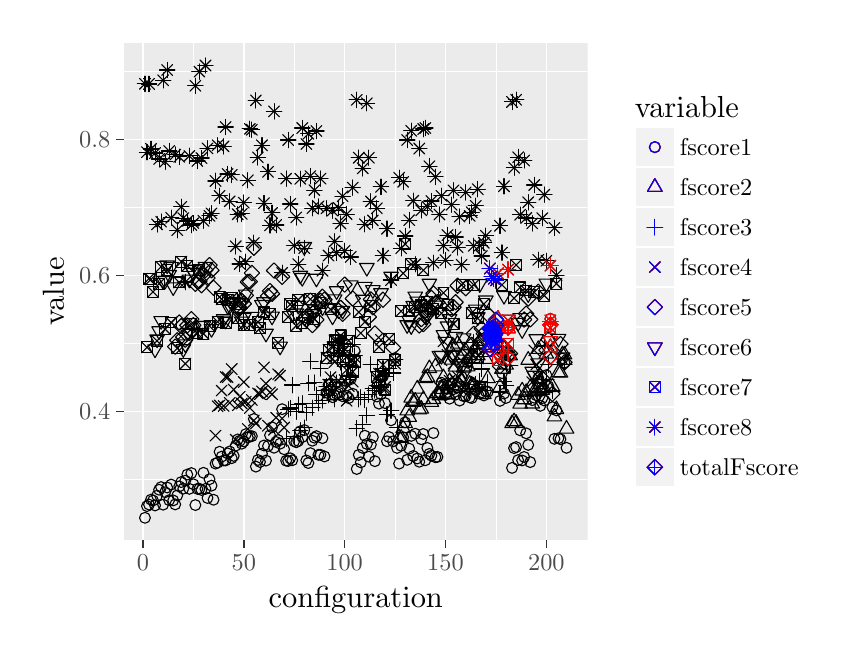
\begin{tikzpicture}[x=1pt,y=1pt]
\definecolor{fillColor}{RGB}{255,255,255}
\path[use as bounding box,fill=fillColor,fill opacity=0.00] (0,0) rectangle (289.08,216.81);
\begin{scope}
\path[clip] (  0.00,  0.00) rectangle (289.08,216.81);
\definecolor{drawColor}{RGB}{255,255,255}
\definecolor{fillColor}{RGB}{255,255,255}

\path[draw=drawColor,line width= 0.6pt,line join=round,line cap=round,fill=fillColor] (  0.00,  0.00) rectangle (289.08,216.81);
\end{scope}
\begin{scope}
\path[clip] ( 34.77, 31.53) rectangle (202.33,211.31);
\definecolor{fillColor}{gray}{0.92}

\path[fill=fillColor] ( 34.77, 31.53) rectangle (202.33,211.31);
\definecolor{drawColor}{RGB}{255,255,255}

\path[draw=drawColor,line width= 0.3pt,line join=round] ( 34.77, 53.51) --
	(202.33, 53.51);

\path[draw=drawColor,line width= 0.3pt,line join=round] ( 34.77,102.66) --
	(202.33,102.66);

\path[draw=drawColor,line width= 0.3pt,line join=round] ( 34.77,151.81) --
	(202.33,151.81);

\path[draw=drawColor,line width= 0.3pt,line join=round] ( 34.77,200.96) --
	(202.33,200.96);

\path[draw=drawColor,line width= 0.3pt,line join=round] ( 59.88, 31.53) --
	( 59.88,211.31);

\path[draw=drawColor,line width= 0.3pt,line join=round] ( 96.32, 31.53) --
	( 96.32,211.31);

\path[draw=drawColor,line width= 0.3pt,line join=round] (132.76, 31.53) --
	(132.76,211.31);

\path[draw=drawColor,line width= 0.3pt,line join=round] (169.20, 31.53) --
	(169.20,211.31);

\path[draw=drawColor,line width= 0.6pt,line join=round] ( 34.77, 78.08) --
	(202.33, 78.08);

\path[draw=drawColor,line width= 0.6pt,line join=round] ( 34.77,127.24) --
	(202.33,127.24);

\path[draw=drawColor,line width= 0.6pt,line join=round] ( 34.77,176.39) --
	(202.33,176.39);

\path[draw=drawColor,line width= 0.6pt,line join=round] ( 41.66, 31.53) --
	( 41.66,211.31);

\path[draw=drawColor,line width= 0.6pt,line join=round] ( 78.10, 31.53) --
	( 78.10,211.31);

\path[draw=drawColor,line width= 0.6pt,line join=round] (114.54, 31.53) --
	(114.54,211.31);

\path[draw=drawColor,line width= 0.6pt,line join=round] (150.98, 31.53) --
	(150.98,211.31);

\path[draw=drawColor,line width= 0.6pt,line join=round] (187.42, 31.53) --
	(187.42,211.31);
\definecolor{drawColor}{RGB}{0,0,0}

\path[draw=drawColor,line width= 0.4pt,line join=round,line cap=round] ( 42.38, 39.70) circle (  1.96);

\path[draw=drawColor,line width= 0.4pt,line join=round,line cap=round] ( 43.11, 43.93) circle (  1.96);

\path[draw=drawColor,line width= 0.4pt,line join=round,line cap=round] ( 43.84, 44.49) circle (  1.96);

\path[draw=drawColor,line width= 0.4pt,line join=round,line cap=round] ( 44.57, 46.26) circle (  1.96);

\path[draw=drawColor,line width= 0.4pt,line join=round,line cap=round] ( 45.30, 45.95) circle (  1.96);

\path[draw=drawColor,line width= 0.4pt,line join=round,line cap=round] ( 46.03, 44.16) circle (  1.96);

\path[draw=drawColor,line width= 0.4pt,line join=round,line cap=round] ( 46.76, 47.70) circle (  1.96);

\path[draw=drawColor,line width= 0.4pt,line join=round,line cap=round] ( 47.49, 49.85) circle (  1.96);

\path[draw=drawColor,line width= 0.4pt,line join=round,line cap=round] ( 48.21, 50.79) circle (  1.96);

\path[draw=drawColor,line width= 0.4pt,line join=round,line cap=round] ( 48.94, 44.44) circle (  1.96);

\path[draw=drawColor,line width= 0.4pt,line join=round,line cap=round] ( 49.67, 48.94) circle (  1.96);

\path[draw=drawColor,line width= 0.4pt,line join=round,line cap=round] ( 50.40, 50.66) circle (  1.96);

\path[draw=drawColor,line width= 0.4pt,line join=round,line cap=round] ( 51.13, 46.07) circle (  1.96);

\path[draw=drawColor,line width= 0.4pt,line join=round,line cap=round] ( 51.86, 51.71) circle (  1.96);

\path[draw=drawColor,line width= 0.4pt,line join=round,line cap=round] ( 52.59, 45.98) circle (  1.96);

\path[draw=drawColor,line width= 0.4pt,line join=round,line cap=round] ( 53.32, 44.54) circle (  1.96);

\path[draw=drawColor,line width= 0.4pt,line join=round,line cap=round] ( 54.05, 47.78) circle (  1.96);

\path[draw=drawColor,line width= 0.4pt,line join=round,line cap=round] ( 54.77, 51.05) circle (  1.96);

\path[draw=drawColor,line width= 0.4pt,line join=round,line cap=round] ( 55.50, 52.62) circle (  1.96);

\path[draw=drawColor,line width= 0.4pt,line join=round,line cap=round] ( 56.23, 50.21) circle (  1.96);

\path[draw=drawColor,line width= 0.4pt,line join=round,line cap=round] ( 56.96, 53.10) circle (  1.96);

\path[draw=drawColor,line width= 0.4pt,line join=round,line cap=round] ( 57.69, 55.33) circle (  1.96);

\path[draw=drawColor,line width= 0.4pt,line join=round,line cap=round] ( 58.42, 50.17) circle (  1.96);

\path[draw=drawColor,line width= 0.4pt,line join=round,line cap=round] ( 59.15, 55.86) circle (  1.96);

\path[draw=drawColor,line width= 0.4pt,line join=round,line cap=round] ( 59.88, 51.83) circle (  1.96);

\path[draw=drawColor,line width= 0.4pt,line join=round,line cap=round] ( 60.60, 44.31) circle (  1.96);

\path[draw=drawColor,line width= 0.4pt,line join=round,line cap=round] ( 61.33, 50.15) circle (  1.96);

\path[draw=drawColor,line width= 0.4pt,line join=round,line cap=round] ( 62.06, 50.19) circle (  1.96);

\path[draw=drawColor,line width= 0.4pt,line join=round,line cap=round] ( 62.79, 49.76) circle (  1.96);

\path[draw=drawColor,line width= 0.4pt,line join=round,line cap=round] ( 63.52, 55.96) circle (  1.96);

\path[draw=drawColor,line width= 0.4pt,line join=round,line cap=round] ( 64.25, 50.14) circle (  1.96);

\path[draw=drawColor,line width= 0.4pt,line join=round,line cap=round] ( 64.98, 46.86) circle (  1.96);

\path[draw=drawColor,line width= 0.4pt,line join=round,line cap=round] ( 65.71, 53.64) circle (  1.96);

\path[draw=drawColor,line width= 0.4pt,line join=round,line cap=round] ( 66.44, 51.32) circle (  1.96);

\path[draw=drawColor,line width= 0.4pt,line join=round,line cap=round] ( 67.16, 46.22) circle (  1.96);

\path[draw=drawColor,line width= 0.4pt,line join=round,line cap=round] ( 67.89, 59.29) circle (  1.96);

\path[draw=drawColor,line width= 0.4pt,line join=round,line cap=round] ( 68.62, 59.62) circle (  1.96);

\path[draw=drawColor,line width= 0.4pt,line join=round,line cap=round] ( 69.35, 63.57) circle (  1.96);

\path[draw=drawColor,line width= 0.4pt,line join=round,line cap=round] ( 70.08, 61.79) circle (  1.96);

\path[draw=drawColor,line width= 0.4pt,line join=round,line cap=round] ( 70.81, 60.39) circle (  1.96);

\path[draw=drawColor,line width= 0.4pt,line join=round,line cap=round] ( 71.54, 60.43) circle (  1.96);

\path[draw=drawColor,line width= 0.4pt,line join=round,line cap=round] ( 72.27, 62.97) circle (  1.96);

\path[draw=drawColor,line width= 0.4pt,line join=round,line cap=round] ( 73.00, 63.67) circle (  1.96);

\path[draw=drawColor,line width= 0.4pt,line join=round,line cap=round] ( 73.72, 61.24) circle (  1.96);

\path[draw=drawColor,line width= 0.4pt,line join=round,line cap=round] ( 74.45, 62.07) circle (  1.96);

\path[draw=drawColor,line width= 0.4pt,line join=round,line cap=round] ( 75.18, 65.77) circle (  1.96);

\path[draw=drawColor,line width= 0.4pt,line join=round,line cap=round] ( 75.91, 68.02) circle (  1.96);

\path[draw=drawColor,line width= 0.4pt,line join=round,line cap=round] ( 76.64, 67.53) circle (  1.96);

\path[draw=drawColor,line width= 0.4pt,line join=round,line cap=round] ( 77.37, 66.48) circle (  1.96);

\path[draw=drawColor,line width= 0.4pt,line join=round,line cap=round] ( 78.10, 67.31) circle (  1.96);

\path[draw=drawColor,line width= 0.4pt,line join=round,line cap=round] ( 78.83, 69.94) circle (  1.96);

\path[draw=drawColor,line width= 0.4pt,line join=round,line cap=round] ( 79.55, 68.71) circle (  1.96);

\path[draw=drawColor,line width= 0.4pt,line join=round,line cap=round] ( 80.28, 69.13) circle (  1.96);

\path[draw=drawColor,line width= 0.4pt,line join=round,line cap=round] ( 81.01, 69.20) circle (  1.96);

\path[draw=drawColor,line width= 0.4pt,line join=round,line cap=round] ( 81.74, 75.40) circle (  1.96);

\path[draw=drawColor,line width= 0.4pt,line join=round,line cap=round] ( 82.47, 58.20) circle (  1.96);

\path[draw=drawColor,line width= 0.4pt,line join=round,line cap=round] ( 83.20, 60.59) circle (  1.96);

\path[draw=drawColor,line width= 0.4pt,line join=round,line cap=round] ( 83.93, 59.87) circle (  1.96);

\path[draw=drawColor,line width= 0.4pt,line join=round,line cap=round] ( 84.66, 62.86) circle (  1.96);

\path[draw=drawColor,line width= 0.4pt,line join=round,line cap=round] ( 85.39, 65.83) circle (  1.96);

\path[draw=drawColor,line width= 0.4pt,line join=round,line cap=round] ( 86.11, 60.38) circle (  1.96);

\path[draw=drawColor,line width= 0.4pt,line join=round,line cap=round] ( 86.84, 65.65) circle (  1.96);

\path[draw=drawColor,line width= 0.4pt,line join=round,line cap=round] ( 87.57, 69.52) circle (  1.96);

\path[draw=drawColor,line width= 0.4pt,line join=round,line cap=round] ( 88.30, 72.40) circle (  1.96);

\path[draw=drawColor,line width= 0.4pt,line join=round,line cap=round] ( 89.03, 65.02) circle (  1.96);

\path[draw=drawColor,line width= 0.4pt,line join=round,line cap=round] ( 89.76, 67.11) circle (  1.96);

\path[draw=drawColor,line width= 0.4pt,line join=round,line cap=round] ( 90.49, 67.80) circle (  1.96);

\path[draw=drawColor,line width= 0.4pt,line join=round,line cap=round] ( 91.22, 66.49) circle (  1.96);

\path[draw=drawColor,line width= 0.4pt,line join=round,line cap=round] ( 91.94, 78.95) circle (  1.96);

\path[draw=drawColor,line width= 0.4pt,line join=round,line cap=round] ( 92.67, 64.47) circle (  1.96);

\path[draw=drawColor,line width= 0.4pt,line join=round,line cap=round] ( 93.40, 60.34) circle (  1.96);

\path[draw=drawColor,line width= 0.4pt,line join=round,line cap=round] ( 94.13, 60.23) circle (  1.96);

\path[draw=drawColor,line width= 0.4pt,line join=round,line cap=round] ( 94.86, 61.22) circle (  1.96);

\path[draw=drawColor,line width= 0.4pt,line join=round,line cap=round] ( 95.59, 60.48) circle (  1.96);

\path[draw=drawColor,line width= 0.4pt,line join=round,line cap=round] ( 96.32, 67.38) circle (  1.96);

\path[draw=drawColor,line width= 0.4pt,line join=round,line cap=round] ( 97.05, 67.00) circle (  1.96);

\path[draw=drawColor,line width= 0.4pt,line join=round,line cap=round] ( 97.78, 67.46) circle (  1.96);

\path[draw=drawColor,line width= 0.4pt,line join=round,line cap=round] ( 98.50, 70.96) circle (  1.96);

\path[draw=drawColor,line width= 0.4pt,line join=round,line cap=round] ( 99.23, 68.87) circle (  1.96);

\path[draw=drawColor,line width= 0.4pt,line join=round,line cap=round] ( 99.96, 71.40) circle (  1.96);

\path[draw=drawColor,line width= 0.4pt,line join=round,line cap=round] (100.69, 60.43) circle (  1.96);

\path[draw=drawColor,line width= 0.4pt,line join=round,line cap=round] (101.42, 59.49) circle (  1.96);

\path[draw=drawColor,line width= 0.4pt,line join=round,line cap=round] (102.15, 63.06) circle (  1.96);

\path[draw=drawColor,line width= 0.4pt,line join=round,line cap=round] (102.88, 67.55) circle (  1.96);

\path[draw=drawColor,line width= 0.4pt,line join=round,line cap=round] (103.61, 68.65) circle (  1.96);

\path[draw=drawColor,line width= 0.4pt,line join=round,line cap=round] (104.34, 69.21) circle (  1.96);

\path[draw=drawColor,line width= 0.4pt,line join=round,line cap=round] (105.06, 62.45) circle (  1.96);

\path[draw=drawColor,line width= 0.4pt,line join=round,line cap=round] (105.79, 62.47) circle (  1.96);

\path[draw=drawColor,line width= 0.4pt,line join=round,line cap=round] (106.52, 68.49) circle (  1.96);

\path[draw=drawColor,line width= 0.4pt,line join=round,line cap=round] (107.25, 61.87) circle (  1.96);

\path[draw=drawColor,line width= 0.4pt,line join=round,line cap=round] (107.98, 84.92) circle (  1.96);

\path[draw=drawColor,line width= 0.4pt,line join=round,line cap=round] (108.71, 87.76) circle (  1.96);

\path[draw=drawColor,line width= 0.4pt,line join=round,line cap=round] (109.44, 85.93) circle (  1.96);

\path[draw=drawColor,line width= 0.4pt,line join=round,line cap=round] (110.17, 83.28) circle (  1.96);

\path[draw=drawColor,line width= 0.4pt,line join=round,line cap=round] (110.89, 84.01) circle (  1.96);

\path[draw=drawColor,line width= 0.4pt,line join=round,line cap=round] (111.62, 84.54) circle (  1.96);

\path[draw=drawColor,line width= 0.4pt,line join=round,line cap=round] (112.35, 84.92) circle (  1.96);

\path[draw=drawColor,line width= 0.4pt,line join=round,line cap=round] (113.08, 86.92) circle (  1.96);

\path[draw=drawColor,line width= 0.4pt,line join=round,line cap=round] (113.81, 83.62) circle (  1.96);

\path[draw=drawColor,line width= 0.4pt,line join=round,line cap=round] (114.54, 89.28) circle (  1.96);

\path[draw=drawColor,line width= 0.4pt,line join=round,line cap=round] (115.27, 83.77) circle (  1.96);

\path[draw=drawColor,line width= 0.4pt,line join=round,line cap=round] (116.00, 82.96) circle (  1.96);

\path[draw=drawColor,line width= 0.4pt,line join=round,line cap=round] (116.73, 89.79) circle (  1.96);

\path[draw=drawColor,line width= 0.4pt,line join=round,line cap=round] (117.45, 84.52) circle (  1.96);

\path[draw=drawColor,line width= 0.4pt,line join=round,line cap=round] (118.18, 99.98) circle (  1.96);

\path[draw=drawColor,line width= 0.4pt,line join=round,line cap=round] (118.91, 57.34) circle (  1.96);

\path[draw=drawColor,line width= 0.4pt,line join=round,line cap=round] (119.64, 62.43) circle (  1.96);

\path[draw=drawColor,line width= 0.4pt,line join=round,line cap=round] (120.37, 59.73) circle (  1.96);

\path[draw=drawColor,line width= 0.4pt,line join=round,line cap=round] (121.10, 64.94) circle (  1.96);

\path[draw=drawColor,line width= 0.4pt,line join=round,line cap=round] (121.83, 69.36) circle (  1.96);

\path[draw=drawColor,line width= 0.4pt,line join=round,line cap=round] (122.56, 66.38) circle (  1.96);

\path[draw=drawColor,line width= 0.4pt,line join=round,line cap=round] (123.28, 61.80) circle (  1.96);

\path[draw=drawColor,line width= 0.4pt,line join=round,line cap=round] (124.01, 66.13) circle (  1.96);

\path[draw=drawColor,line width= 0.4pt,line join=round,line cap=round] (124.74, 68.81) circle (  1.96);

\path[draw=drawColor,line width= 0.4pt,line join=round,line cap=round] (125.47, 60.16) circle (  1.96);

\path[draw=drawColor,line width= 0.4pt,line join=round,line cap=round] (126.20, 83.53) circle (  1.96);

\path[draw=drawColor,line width= 0.4pt,line join=round,line cap=round] (126.93, 80.96) circle (  1.96);

\path[draw=drawColor,line width= 0.4pt,line join=round,line cap=round] (127.66, 84.34) circle (  1.96);

\path[draw=drawColor,line width= 0.4pt,line join=round,line cap=round] (128.39, 90.81) circle (  1.96);

\path[draw=drawColor,line width= 0.4pt,line join=round,line cap=round] (129.12, 81.16) circle (  1.96);

\path[draw=drawColor,line width= 0.4pt,line join=round,line cap=round] (129.84, 67.36) circle (  1.96);

\path[draw=drawColor,line width= 0.4pt,line join=round,line cap=round] (130.57, 68.90) circle (  1.96);

\path[draw=drawColor,line width= 0.4pt,line join=round,line cap=round] (131.30, 74.92) circle (  1.96);

\path[draw=drawColor,line width= 0.4pt,line join=round,line cap=round] (132.03, 67.33) circle (  1.96);

\path[draw=drawColor,line width= 0.4pt,line join=round,line cap=round] (132.76, 97.43) circle (  1.96);

\path[draw=drawColor,line width= 0.4pt,line join=round,line cap=round] (133.49, 64.96) circle (  1.96);

\path[draw=drawColor,line width= 0.4pt,line join=round,line cap=round] (134.22, 59.28) circle (  1.96);

\path[draw=drawColor,line width= 0.4pt,line join=round,line cap=round] (134.95, 65.72) circle (  1.96);

\path[draw=drawColor,line width= 0.4pt,line join=round,line cap=round] (135.68, 68.82) circle (  1.96);

\path[draw=drawColor,line width= 0.4pt,line join=round,line cap=round] (136.40, 74.21) circle (  1.96);

\path[draw=drawColor,line width= 0.4pt,line join=round,line cap=round] (137.13, 60.65) circle (  1.96);

\path[draw=drawColor,line width= 0.4pt,line join=round,line cap=round] (137.86, 64.70) circle (  1.96);

\path[draw=drawColor,line width= 0.4pt,line join=round,line cap=round] (138.59, 69.30) circle (  1.96);

\path[draw=drawColor,line width= 0.4pt,line join=round,line cap=round] (139.32, 62.04) circle (  1.96);

\path[draw=drawColor,line width= 0.4pt,line join=round,line cap=round] (140.05, 70.08) circle (  1.96);

\path[draw=drawColor,line width= 0.4pt,line join=round,line cap=round] (140.78, 61.13) circle (  1.96);

\path[draw=drawColor,line width= 0.4pt,line join=round,line cap=round] (141.51, 59.95) circle (  1.96);

\path[draw=drawColor,line width= 0.4pt,line join=round,line cap=round] (142.23, 68.08) circle (  1.96);

\path[draw=drawColor,line width= 0.4pt,line join=round,line cap=round] (142.96, 69.99) circle (  1.96);

\path[draw=drawColor,line width= 0.4pt,line join=round,line cap=round] (143.69, 60.49) circle (  1.96);

\path[draw=drawColor,line width= 0.4pt,line join=round,line cap=round] (144.42, 64.95) circle (  1.96);

\path[draw=drawColor,line width= 0.4pt,line join=round,line cap=round] (145.15, 62.80) circle (  1.96);

\path[draw=drawColor,line width= 0.4pt,line join=round,line cap=round] (145.88, 62.16) circle (  1.96);

\path[draw=drawColor,line width= 0.4pt,line join=round,line cap=round] (146.61, 70.33) circle (  1.96);

\path[draw=drawColor,line width= 0.4pt,line join=round,line cap=round] (147.34, 61.57) circle (  1.96);

\path[draw=drawColor,line width= 0.4pt,line join=round,line cap=round] (148.07, 61.71) circle (  1.96);

\path[draw=drawColor,line width= 0.4pt,line join=round,line cap=round] (148.79, 85.06) circle (  1.96);

\path[draw=drawColor,line width= 0.4pt,line join=round,line cap=round] (149.52, 88.51) circle (  1.96);

\path[draw=drawColor,line width= 0.4pt,line join=round,line cap=round] (150.25, 87.75) circle (  1.96);

\path[draw=drawColor,line width= 0.4pt,line join=round,line cap=round] (150.98, 84.11) circle (  1.96);

\path[draw=drawColor,line width= 0.4pt,line join=round,line cap=round] (151.71, 85.14) circle (  1.96);

\path[draw=drawColor,line width= 0.4pt,line join=round,line cap=round] (152.44, 82.74) circle (  1.96);

\path[draw=drawColor,line width= 0.4pt,line join=round,line cap=round] (153.17, 88.21) circle (  1.96);

\path[draw=drawColor,line width= 0.4pt,line join=round,line cap=round] (153.90, 86.20) circle (  1.96);

\path[draw=drawColor,line width= 0.4pt,line join=round,line cap=round] (154.62, 84.20) circle (  1.96);

\path[draw=drawColor,line width= 0.4pt,line join=round,line cap=round] (155.35, 86.81) circle (  1.96);

\path[draw=drawColor,line width= 0.4pt,line join=round,line cap=round] (156.08, 82.06) circle (  1.96);

\path[draw=drawColor,line width= 0.4pt,line join=round,line cap=round] (156.81, 90.63) circle (  1.96);

\path[draw=drawColor,line width= 0.4pt,line join=round,line cap=round] (157.54, 83.65) circle (  1.96);

\path[draw=drawColor,line width= 0.4pt,line join=round,line cap=round] (158.27, 83.66) circle (  1.96);

\path[draw=drawColor,line width= 0.4pt,line join=round,line cap=round] (159.00, 95.76) circle (  1.96);

\path[draw=drawColor,line width= 0.4pt,line join=round,line cap=round] (159.73, 83.21) circle (  1.96);

\path[draw=drawColor,line width= 0.4pt,line join=round,line cap=round] (160.46, 82.97) circle (  1.96);

\path[draw=drawColor,line width= 0.4pt,line join=round,line cap=round] (161.18, 87.87) circle (  1.96);

\path[draw=drawColor,line width= 0.4pt,line join=round,line cap=round] (161.91, 85.74) circle (  1.96);

\path[draw=drawColor,line width= 0.4pt,line join=round,line cap=round] (162.64, 86.58) circle (  1.96);

\path[draw=drawColor,line width= 0.4pt,line join=round,line cap=round] (163.37, 87.27) circle (  1.96);

\path[draw=drawColor,line width= 0.4pt,line join=round,line cap=round] (164.10, 85.05) circle (  1.96);

\path[draw=drawColor,line width= 0.4pt,line join=round,line cap=round] (164.83, 83.91) circle (  1.96);

\path[draw=drawColor,line width= 0.4pt,line join=round,line cap=round] (165.56, 85.37) circle (  1.96);

\path[draw=drawColor,line width= 0.4pt,line join=round,line cap=round] (166.29, 85.28) circle (  1.96);

\path[draw=drawColor,line width= 0.4pt,line join=round,line cap=round] (167.02,101.52) circle (  1.96);

\path[draw=drawColor,line width= 0.4pt,line join=round,line cap=round] (167.74,107.48) circle (  1.96);

\path[draw=drawColor,line width= 0.4pt,line join=round,line cap=round] (168.47,107.05) circle (  1.96);

\path[draw=drawColor,line width= 0.4pt,line join=round,line cap=round] (169.20,107.16) circle (  1.96);

\path[draw=drawColor,line width= 0.4pt,line join=round,line cap=round] (169.93,108.25) circle (  1.96);

\path[draw=drawColor,line width= 0.4pt,line join=round,line cap=round] (170.66, 81.96) circle (  1.96);

\path[draw=drawColor,line width= 0.4pt,line join=round,line cap=round] (171.39, 91.98) circle (  1.96);

\path[draw=drawColor,line width= 0.4pt,line join=round,line cap=round] (172.12, 84.60) circle (  1.96);

\path[draw=drawColor,line width= 0.4pt,line join=round,line cap=round] (172.85, 83.00) circle (  1.96);

\path[draw=drawColor,line width= 0.4pt,line join=round,line cap=round] (173.57,109.14) circle (  1.96);

\path[draw=drawColor,line width= 0.4pt,line join=round,line cap=round] (174.30, 98.49) circle (  1.96);

\path[draw=drawColor,line width= 0.4pt,line join=round,line cap=round] (175.03, 57.74) circle (  1.96);

\path[draw=drawColor,line width= 0.4pt,line join=round,line cap=round] (175.76, 64.88) circle (  1.96);

\path[draw=drawColor,line width= 0.4pt,line join=round,line cap=round] (176.49, 65.26) circle (  1.96);

\path[draw=drawColor,line width= 0.4pt,line join=round,line cap=round] (177.22, 60.55) circle (  1.96);

\path[draw=drawColor,line width= 0.4pt,line join=round,line cap=round] (177.95, 71.30) circle (  1.96);

\path[draw=drawColor,line width= 0.4pt,line join=round,line cap=round] (178.68, 60.42) circle (  1.96);

\path[draw=drawColor,line width= 0.4pt,line join=round,line cap=round] (179.41, 61.68) circle (  1.96);

\path[draw=drawColor,line width= 0.4pt,line join=round,line cap=round] (180.13, 70.23) circle (  1.96);

\path[draw=drawColor,line width= 0.4pt,line join=round,line cap=round] (180.86, 66.05) circle (  1.96);

\path[draw=drawColor,line width= 0.4pt,line join=round,line cap=round] (181.59, 59.83) circle (  1.96);

\path[draw=drawColor,line width= 0.4pt,line join=round,line cap=round] (182.32, 82.23) circle (  1.96);

\path[draw=drawColor,line width= 0.4pt,line join=round,line cap=round] (183.05, 83.11) circle (  1.96);

\path[draw=drawColor,line width= 0.4pt,line join=round,line cap=round] (183.78, 83.99) circle (  1.96);

\path[draw=drawColor,line width= 0.4pt,line join=round,line cap=round] (184.51, 90.22) circle (  1.96);

\path[draw=drawColor,line width= 0.4pt,line join=round,line cap=round] (185.24, 80.16) circle (  1.96);

\path[draw=drawColor,line width= 0.4pt,line join=round,line cap=round] (185.96, 82.96) circle (  1.96);

\path[draw=drawColor,line width= 0.4pt,line join=round,line cap=round] (186.69, 82.09) circle (  1.96);

\path[draw=drawColor,line width= 0.4pt,line join=round,line cap=round] (187.42, 91.25) circle (  1.96);

\path[draw=drawColor,line width= 0.4pt,line join=round,line cap=round] (188.15, 87.21) circle (  1.96);

\path[draw=drawColor,line width= 0.4pt,line join=round,line cap=round] (188.88,111.60) circle (  1.96);

\path[draw=drawColor,line width= 0.4pt,line join=round,line cap=round] (189.61, 79.69) circle (  1.96);

\path[draw=drawColor,line width= 0.4pt,line join=round,line cap=round] (190.34, 68.24) circle (  1.96);

\path[draw=drawColor,line width= 0.4pt,line join=round,line cap=round] (191.07, 78.51) circle (  1.96);

\path[draw=drawColor,line width= 0.4pt,line join=round,line cap=round] (191.80, 68.44) circle (  1.96);

\path[draw=drawColor,line width= 0.4pt,line join=round,line cap=round] (192.52, 68.11) circle (  1.96);

\path[draw=drawColor,line width= 0.4pt,line join=round,line cap=round] (193.25, 97.26) circle (  1.96);

\path[draw=drawColor,line width= 0.4pt,line join=round,line cap=round] (193.98, 95.76) circle (  1.96);

\path[draw=drawColor,line width= 0.4pt,line join=round,line cap=round] (194.71, 64.99) circle (  1.96);

\path[draw=drawColor,line width= 0.4pt,line join=round,line cap=round] (134.22, 71.71) --
	(136.86, 67.13) --
	(131.57, 67.13) --
	(134.22, 71.71);

\path[draw=drawColor,line width= 0.4pt,line join=round,line cap=round] (134.95, 71.58) --
	(137.59, 67.00) --
	(132.30, 67.00) --
	(134.95, 71.58);

\path[draw=drawColor,line width= 0.4pt,line join=round,line cap=round] (135.68, 75.06) --
	(138.32, 70.48) --
	(133.03, 70.48) --
	(135.68, 75.06);

\path[draw=drawColor,line width= 0.4pt,line join=round,line cap=round] (136.40, 76.85) --
	(139.05, 72.28) --
	(133.76, 72.28) --
	(136.40, 76.85);

\path[draw=drawColor,line width= 0.4pt,line join=round,line cap=round] (137.13, 81.45) --
	(139.78, 76.87) --
	(134.49, 76.87) --
	(137.13, 81.45);

\path[draw=drawColor,line width= 0.4pt,line join=round,line cap=round] (137.86, 79.13) --
	(140.50, 74.55) --
	(135.22, 74.55) --
	(137.86, 79.13);

\path[draw=drawColor,line width= 0.4pt,line join=round,line cap=round] (138.59, 86.09) --
	(141.23, 81.51) --
	(135.95, 81.51) --
	(138.59, 86.09);

\path[draw=drawColor,line width= 0.4pt,line join=round,line cap=round] (139.32, 84.52) --
	(141.96, 79.94) --
	(136.68, 79.94) --
	(139.32, 84.52);

\path[draw=drawColor,line width= 0.4pt,line join=round,line cap=round] (140.05, 84.95) --
	(142.69, 80.37) --
	(137.41, 80.37) --
	(140.05, 84.95);

\path[draw=drawColor,line width= 0.4pt,line join=round,line cap=round] (140.78, 89.34) --
	(143.42, 84.76) --
	(138.13, 84.76) --
	(140.78, 89.34);

\path[draw=drawColor,line width= 0.4pt,line join=round,line cap=round] (141.51, 81.85) --
	(144.15, 77.27) --
	(138.86, 77.27) --
	(141.51, 81.85);

\path[draw=drawColor,line width= 0.4pt,line join=round,line cap=round] (142.23, 82.09) --
	(144.88, 77.51) --
	(139.59, 77.51) --
	(142.23, 82.09);

\path[draw=drawColor,line width= 0.4pt,line join=round,line cap=round] (142.96, 85.51) --
	(145.61, 80.94) --
	(140.32, 80.94) --
	(142.96, 85.51);

\path[draw=drawColor,line width= 0.4pt,line join=round,line cap=round] (143.69, 93.14) --
	(146.33, 88.56) --
	(141.05, 88.56) --
	(143.69, 93.14);

\path[draw=drawColor,line width= 0.4pt,line join=round,line cap=round] (144.42, 93.55) --
	(147.06, 88.97) --
	(141.78, 88.97) --
	(144.42, 93.55);

\path[draw=drawColor,line width= 0.4pt,line join=round,line cap=round] (145.15, 96.72) --
	(147.79, 92.14) --
	(142.51, 92.14) --
	(145.15, 96.72);

\path[draw=drawColor,line width= 0.4pt,line join=round,line cap=round] (145.88, 84.53) --
	(148.52, 79.95) --
	(143.24, 79.95) --
	(145.88, 84.53);

\path[draw=drawColor,line width= 0.4pt,line join=round,line cap=round] (146.61, 85.57) --
	(149.25, 80.99) --
	(143.97, 80.99) --
	(146.61, 85.57);

\path[draw=drawColor,line width= 0.4pt,line join=round,line cap=round] (147.34, 97.39) --
	(149.98, 92.81) --
	(144.69, 92.81) --
	(147.34, 97.39);

\path[draw=drawColor,line width= 0.4pt,line join=round,line cap=round] (148.07, 87.67) --
	(150.71, 83.09) --
	(145.42, 83.09) --
	(148.07, 87.67);

\path[draw=drawColor,line width= 0.4pt,line join=round,line cap=round] (148.79, 86.93) --
	(151.44, 82.35) --
	(146.15, 82.35) --
	(148.79, 86.93);

\path[draw=drawColor,line width= 0.4pt,line join=round,line cap=round] (149.52, 89.21) --
	(152.17, 84.64) --
	(146.88, 84.64) --
	(149.52, 89.21);

\path[draw=drawColor,line width= 0.4pt,line join=round,line cap=round] (150.25, 93.41) --
	(152.89, 88.83) --
	(147.61, 88.83) --
	(150.25, 93.41);

\path[draw=drawColor,line width= 0.4pt,line join=round,line cap=round] (150.98, 87.25) --
	(153.62, 82.68) --
	(148.34, 82.68) --
	(150.98, 87.25);

\path[draw=drawColor,line width= 0.4pt,line join=round,line cap=round] (151.71, 87.30) --
	(154.35, 82.72) --
	(149.07, 82.72) --
	(151.71, 87.30);

\path[draw=drawColor,line width= 0.4pt,line join=round,line cap=round] (152.44, 92.07) --
	(155.08, 87.50) --
	(149.80, 87.50) --
	(152.44, 92.07);

\path[draw=drawColor,line width= 0.4pt,line join=round,line cap=round] (153.17, 99.82) --
	(155.81, 95.24) --
	(150.52, 95.24) --
	(153.17, 99.82);

\path[draw=drawColor,line width= 0.4pt,line join=round,line cap=round] (153.90,104.61) --
	(156.54,100.04) --
	(151.25,100.04) --
	(153.90,104.61);

\path[draw=drawColor,line width= 0.4pt,line join=round,line cap=round] (154.62, 97.27) --
	(157.27, 92.69) --
	(151.98, 92.69) --
	(154.62, 97.27);

\path[draw=drawColor,line width= 0.4pt,line join=round,line cap=round] (155.35,105.61) --
	(158.00,101.03) --
	(152.71,101.03) --
	(155.35,105.61);

\path[draw=drawColor,line width= 0.4pt,line join=round,line cap=round] (156.08, 90.44) --
	(158.73, 85.86) --
	(153.44, 85.86) --
	(156.08, 90.44);

\path[draw=drawColor,line width= 0.4pt,line join=round,line cap=round] (156.81, 91.91) --
	(159.45, 87.33) --
	(154.17, 87.33) --
	(156.81, 91.91);

\path[draw=drawColor,line width= 0.4pt,line join=round,line cap=round] (157.54, 96.95) --
	(160.18, 92.38) --
	(154.90, 92.38) --
	(157.54, 96.95);

\path[draw=drawColor,line width= 0.4pt,line join=round,line cap=round] (158.27,103.06) --
	(160.91, 98.49) --
	(155.63, 98.49) --
	(158.27,103.06);

\path[draw=drawColor,line width= 0.4pt,line join=round,line cap=round] (159.00, 97.35) --
	(161.64, 92.78) --
	(156.36, 92.78) --
	(159.00, 97.35);

\path[draw=drawColor,line width= 0.4pt,line join=round,line cap=round] (159.73, 91.08) --
	(162.37, 86.51) --
	(157.08, 86.51) --
	(159.73, 91.08);

\path[draw=drawColor,line width= 0.4pt,line join=round,line cap=round] (160.46, 90.78) --
	(163.10, 86.20) --
	(157.81, 86.20) --
	(160.46, 90.78);

\path[draw=drawColor,line width= 0.4pt,line join=round,line cap=round] (161.18, 90.45) --
	(163.83, 85.87) --
	(158.54, 85.87) --
	(161.18, 90.45);

\path[draw=drawColor,line width= 0.4pt,line join=round,line cap=round] (161.91,100.19) --
	(164.56, 95.62) --
	(159.27, 95.62) --
	(161.91,100.19);

\path[draw=drawColor,line width= 0.4pt,line join=round,line cap=round] (162.64,101.39) --
	(165.28, 96.81) --
	(160.00, 96.81) --
	(162.64,101.39);

\path[draw=drawColor,line width= 0.4pt,line join=round,line cap=round] (163.37,106.64) --
	(166.01,102.07) --
	(160.73,102.07) --
	(163.37,106.64);

\path[draw=drawColor,line width= 0.4pt,line join=round,line cap=round] (164.10, 87.36) --
	(166.74, 82.78) --
	(161.46, 82.78) --
	(164.10, 87.36);

\path[draw=drawColor,line width= 0.4pt,line join=round,line cap=round] (164.83, 87.39) --
	(167.47, 82.81) --
	(162.19, 82.81) --
	(164.83, 87.39);

\path[draw=drawColor,line width= 0.4pt,line join=round,line cap=round] (165.56,100.07) --
	(168.20, 95.49) --
	(162.91, 95.49) --
	(165.56,100.07);

\path[draw=drawColor,line width= 0.4pt,line join=round,line cap=round] (166.29, 93.12) --
	(168.93, 88.54) --
	(163.64, 88.54) --
	(166.29, 93.12);

\path[draw=drawColor,line width= 0.4pt,line join=round,line cap=round] (167.02,110.08) --
	(169.66,105.50) --
	(164.37,105.50) --
	(167.02,110.08);

\path[draw=drawColor,line width= 0.4pt,line join=round,line cap=round] (167.74,105.13) --
	(170.39,100.55) --
	(165.10,100.55) --
	(167.74,105.13);

\path[draw=drawColor,line width= 0.4pt,line join=round,line cap=round] (168.47,109.17) --
	(171.12,104.59) --
	(165.83,104.59) --
	(168.47,109.17);

\path[draw=drawColor,line width= 0.4pt,line join=round,line cap=round] (169.20,108.04) --
	(171.84,103.46) --
	(166.56,103.46) --
	(169.20,108.04);

\path[draw=drawColor,line width= 0.4pt,line join=round,line cap=round] (169.93,114.58) --
	(172.57,110.00) --
	(167.29,110.00) --
	(169.93,114.58);

\path[draw=drawColor,line width= 0.4pt,line join=round,line cap=round] (170.66, 89.96) --
	(173.30, 85.39) --
	(168.02, 85.39) --
	(170.66, 89.96);

\path[draw=drawColor,line width= 0.4pt,line join=round,line cap=round] (171.39, 96.51) --
	(174.03, 91.93) --
	(168.75, 91.93) --
	(171.39, 96.51);

\path[draw=drawColor,line width= 0.4pt,line join=round,line cap=round] (172.12,103.83) --
	(174.76, 99.25) --
	(169.47, 99.25) --
	(172.12,103.83);

\path[draw=drawColor,line width= 0.4pt,line join=round,line cap=round] (172.85, 98.03) --
	(175.49, 93.45) --
	(170.20, 93.45) --
	(172.85, 98.03);

\path[draw=drawColor,line width= 0.4pt,line join=round,line cap=round] (173.57,111.14) --
	(176.22,106.56) --
	(170.93,106.56) --
	(173.57,111.14);

\path[draw=drawColor,line width= 0.4pt,line join=round,line cap=round] (174.30,101.41) --
	(176.95, 96.83) --
	(171.66, 96.83) --
	(174.30,101.41);

\path[draw=drawColor,line width= 0.4pt,line join=round,line cap=round] (175.03, 76.84) --
	(177.67, 72.27) --
	(172.39, 72.27) --
	(175.03, 76.84);

\path[draw=drawColor,line width= 0.4pt,line join=round,line cap=round] (175.76, 77.54) --
	(178.40, 72.96) --
	(173.12, 72.96) --
	(175.76, 77.54);

\path[draw=drawColor,line width= 0.4pt,line join=round,line cap=round] (176.49, 76.96) --
	(179.13, 72.39) --
	(173.85, 72.39) --
	(176.49, 76.96);

\path[draw=drawColor,line width= 0.4pt,line join=round,line cap=round] (177.22, 87.07) --
	(179.86, 82.50) --
	(174.58, 82.50) --
	(177.22, 87.07);

\path[draw=drawColor,line width= 0.4pt,line join=round,line cap=round] (177.95, 83.91) --
	(180.59, 79.33) --
	(175.31, 79.33) --
	(177.95, 83.91);

\path[draw=drawColor,line width= 0.4pt,line join=round,line cap=round] (178.68, 88.67) --
	(181.32, 84.09) --
	(176.03, 84.09) --
	(178.68, 88.67);

\path[draw=drawColor,line width= 0.4pt,line join=round,line cap=round] (179.41, 85.49) --
	(182.05, 80.91) --
	(176.76, 80.91) --
	(179.41, 85.49);

\path[draw=drawColor,line width= 0.4pt,line join=round,line cap=round] (180.13, 88.12) --
	(182.78, 83.54) --
	(177.49, 83.54) --
	(180.13, 88.12);

\path[draw=drawColor,line width= 0.4pt,line join=round,line cap=round] (180.86, 99.78) --
	(183.51, 95.20) --
	(178.22, 95.20) --
	(180.86, 99.78);

\path[draw=drawColor,line width= 0.4pt,line join=round,line cap=round] (181.59, 89.74) --
	(184.23, 85.17) --
	(178.95, 85.17) --
	(181.59, 89.74);

\path[draw=drawColor,line width= 0.4pt,line join=round,line cap=round] (182.32, 83.97) --
	(184.96, 79.39) --
	(179.68, 79.39) --
	(182.32, 83.97);

\path[draw=drawColor,line width= 0.4pt,line join=round,line cap=round] (183.05, 88.53) --
	(185.69, 83.95) --
	(180.41, 83.95) --
	(183.05, 88.53);

\path[draw=drawColor,line width= 0.4pt,line join=round,line cap=round] (183.78, 88.57) --
	(186.42, 83.99) --
	(181.14, 83.99) --
	(183.78, 88.57);

\path[draw=drawColor,line width= 0.4pt,line join=round,line cap=round] (184.51,103.67) --
	(187.15, 99.10) --
	(181.86, 99.10) --
	(184.51,103.67);

\path[draw=drawColor,line width= 0.4pt,line join=round,line cap=round] (185.24, 90.93) --
	(187.88, 86.35) --
	(182.59, 86.35) --
	(185.24, 90.93);

\path[draw=drawColor,line width= 0.4pt,line join=round,line cap=round] (185.96, 88.93) --
	(188.61, 84.35) --
	(183.32, 84.35) --
	(185.96, 88.93);

\path[draw=drawColor,line width= 0.4pt,line join=round,line cap=round] (186.69, 89.49) --
	(189.34, 84.91) --
	(184.05, 84.91) --
	(186.69, 89.49);

\path[draw=drawColor,line width= 0.4pt,line join=round,line cap=round] (187.42,101.96) --
	(190.06, 97.38) --
	(184.78, 97.38) --
	(187.42,101.96);

\path[draw=drawColor,line width= 0.4pt,line join=round,line cap=round] (188.15, 89.85) --
	(190.79, 85.28) --
	(185.51, 85.28) --
	(188.15, 89.85);

\path[draw=drawColor,line width= 0.4pt,line join=round,line cap=round] (188.88,104.34) --
	(191.52, 99.76) --
	(186.24, 99.76) --
	(188.88,104.34);

\path[draw=drawColor,line width= 0.4pt,line join=round,line cap=round] (189.61, 90.15) --
	(192.25, 85.57) --
	(186.97, 85.57) --
	(189.61, 90.15);

\path[draw=drawColor,line width= 0.4pt,line join=round,line cap=round] (190.34, 79.28) --
	(192.98, 74.70) --
	(187.70, 74.70) --
	(190.34, 79.28);

\path[draw=drawColor,line width= 0.4pt,line join=round,line cap=round] (191.07, 81.93) --
	(193.71, 77.35) --
	(188.42, 77.35) --
	(191.07, 81.93);

\path[draw=drawColor,line width= 0.4pt,line join=round,line cap=round] (191.80, 95.25) --
	(194.44, 90.68) --
	(189.15, 90.68) --
	(191.80, 95.25);

\path[draw=drawColor,line width= 0.4pt,line join=round,line cap=round] (192.52, 95.14) --
	(195.17, 90.56) --
	(189.88, 90.56) --
	(192.52, 95.14);

\path[draw=drawColor,line width= 0.4pt,line join=round,line cap=round] (193.25,101.71) --
	(195.90, 97.13) --
	(190.61, 97.13) --
	(193.25,101.71);

\path[draw=drawColor,line width= 0.4pt,line join=round,line cap=round] (193.98,101.69) --
	(196.62, 97.11) --
	(191.34, 97.11) --
	(193.98,101.69);

\path[draw=drawColor,line width= 0.4pt,line join=round,line cap=round] (194.71, 74.88) --
	(197.35, 70.30) --
	(192.07, 70.30) --
	(194.71, 74.88);

\path[draw=drawColor,line width= 0.4pt,line join=round,line cap=round] ( 90.63, 68.27) -- ( 96.18, 68.27);

\path[draw=drawColor,line width= 0.4pt,line join=round,line cap=round] ( 93.40, 65.50) -- ( 93.40, 71.05);

\path[draw=drawColor,line width= 0.4pt,line join=round,line cap=round] ( 91.36, 78.88) -- ( 96.91, 78.88);

\path[draw=drawColor,line width= 0.4pt,line join=round,line cap=round] ( 94.13, 76.10) -- ( 94.13, 81.65);

\path[draw=drawColor,line width= 0.4pt,line join=round,line cap=round] ( 92.09, 79.37) -- ( 97.64, 79.37);

\path[draw=drawColor,line width= 0.4pt,line join=round,line cap=round] ( 94.86, 76.60) -- ( 94.86, 82.15);

\path[draw=drawColor,line width= 0.4pt,line join=round,line cap=round] ( 92.81, 87.67) -- ( 98.36, 87.67);

\path[draw=drawColor,line width= 0.4pt,line join=round,line cap=round] ( 95.59, 84.89) -- ( 95.59, 90.44);

\path[draw=drawColor,line width= 0.4pt,line join=round,line cap=round] ( 93.54, 68.92) -- ( 99.09, 68.92);

\path[draw=drawColor,line width= 0.4pt,line join=round,line cap=round] ( 96.32, 66.14) -- ( 96.32, 71.69);

\path[draw=drawColor,line width= 0.4pt,line join=round,line cap=round] ( 94.27, 78.08) -- ( 99.82, 78.08);

\path[draw=drawColor,line width= 0.4pt,line join=round,line cap=round] ( 97.05, 75.31) -- ( 97.05, 80.86);

\path[draw=drawColor,line width= 0.4pt,line join=round,line cap=round] ( 95.00, 80.57) -- (100.55, 80.57);

\path[draw=drawColor,line width= 0.4pt,line join=round,line cap=round] ( 97.78, 77.79) -- ( 97.78, 83.34);

\path[draw=drawColor,line width= 0.4pt,line join=round,line cap=round] ( 95.73, 71.29) -- (101.28, 71.29);

\path[draw=drawColor,line width= 0.4pt,line join=round,line cap=round] ( 98.50, 68.52) -- ( 98.50, 74.07);

\path[draw=drawColor,line width= 0.4pt,line join=round,line cap=round] ( 96.46, 81.06) -- (102.01, 81.06);

\path[draw=drawColor,line width= 0.4pt,line join=round,line cap=round] ( 99.23, 78.29) -- ( 99.23, 83.84);

\path[draw=drawColor,line width= 0.4pt,line join=round,line cap=round] ( 97.19, 72.26) -- (102.74, 72.26);

\path[draw=drawColor,line width= 0.4pt,line join=round,line cap=round] ( 99.96, 69.48) -- ( 99.96, 75.03);

\path[draw=drawColor,line width= 0.4pt,line join=round,line cap=round] ( 97.92, 77.71) -- (103.47, 77.71);

\path[draw=drawColor,line width= 0.4pt,line join=round,line cap=round] (100.69, 74.94) -- (100.69, 80.49);

\path[draw=drawColor,line width= 0.4pt,line join=round,line cap=round] ( 98.64, 88.38) -- (104.19, 88.38);

\path[draw=drawColor,line width= 0.4pt,line join=round,line cap=round] (101.42, 85.60) -- (101.42, 91.15);

\path[draw=drawColor,line width= 0.4pt,line join=round,line cap=round] ( 99.37, 96.21) -- (104.92, 96.21);

\path[draw=drawColor,line width= 0.4pt,line join=round,line cap=round] (102.15, 93.43) -- (102.15, 98.98);

\path[draw=drawColor,line width= 0.4pt,line join=round,line cap=round] (100.10, 79.47) -- (105.65, 79.47);

\path[draw=drawColor,line width= 0.4pt,line join=round,line cap=round] (102.88, 76.69) -- (102.88, 82.24);

\path[draw=drawColor,line width= 0.4pt,line join=round,line cap=round] (100.83, 88.56) -- (106.38, 88.56);

\path[draw=drawColor,line width= 0.4pt,line join=round,line cap=round] (103.61, 85.78) -- (103.61, 91.33);

\path[draw=drawColor,line width= 0.4pt,line join=round,line cap=round] (101.56, 84.14) -- (107.11, 84.14);

\path[draw=drawColor,line width= 0.4pt,line join=round,line cap=round] (104.34, 81.36) -- (104.34, 86.91);

\path[draw=drawColor,line width= 0.4pt,line join=round,line cap=round] (102.29, 81.09) -- (107.84, 81.09);

\path[draw=drawColor,line width= 0.4pt,line join=round,line cap=round] (105.06, 78.32) -- (105.06, 83.87);

\path[draw=drawColor,line width= 0.4pt,line join=round,line cap=round] (103.02, 93.66) -- (108.57, 93.66);

\path[draw=drawColor,line width= 0.4pt,line join=round,line cap=round] (105.79, 90.89) -- (105.79, 96.44);

\path[draw=drawColor,line width= 0.4pt,line join=round,line cap=round] (103.75, 82.15) -- (109.30, 82.15);

\path[draw=drawColor,line width= 0.4pt,line join=round,line cap=round] (106.52, 79.37) -- (106.52, 84.92);

\path[draw=drawColor,line width= 0.4pt,line join=round,line cap=round] (104.48, 85.77) -- (110.03, 85.77);

\path[draw=drawColor,line width= 0.4pt,line join=round,line cap=round] (107.25, 82.99) -- (107.25, 88.54);

\path[draw=drawColor,line width= 0.4pt,line join=round,line cap=round] (105.20, 87.27) -- (110.75, 87.27);

\path[draw=drawColor,line width= 0.4pt,line join=round,line cap=round] (107.98, 84.49) -- (107.98, 90.04);

\path[draw=drawColor,line width= 0.4pt,line join=round,line cap=round] (105.93, 84.03) -- (111.48, 84.03);

\path[draw=drawColor,line width= 0.4pt,line join=round,line cap=round] (108.71, 81.26) -- (108.71, 86.81);

\path[draw=drawColor,line width= 0.4pt,line join=round,line cap=round] (106.66, 89.75) -- (112.21, 89.75);

\path[draw=drawColor,line width= 0.4pt,line join=round,line cap=round] (109.44, 86.97) -- (109.44, 92.52);

\path[draw=drawColor,line width= 0.4pt,line join=round,line cap=round] (107.39, 87.16) -- (112.94, 87.16);

\path[draw=drawColor,line width= 0.4pt,line join=round,line cap=round] (110.17, 84.38) -- (110.17, 89.93);

\path[draw=drawColor,line width= 0.4pt,line join=round,line cap=round] (108.12, 82.54) -- (113.67, 82.54);

\path[draw=drawColor,line width= 0.4pt,line join=round,line cap=round] (110.89, 79.76) -- (110.89, 85.31);

\path[draw=drawColor,line width= 0.4pt,line join=round,line cap=round] (108.85, 88.51) -- (114.40, 88.51);

\path[draw=drawColor,line width= 0.4pt,line join=round,line cap=round] (111.62, 85.74) -- (111.62, 91.29);

\path[draw=drawColor,line width= 0.4pt,line join=round,line cap=round] (109.58, 99.25) -- (115.13, 99.25);

\path[draw=drawColor,line width= 0.4pt,line join=round,line cap=round] (112.35, 96.47) -- (112.35,102.02);

\path[draw=drawColor,line width= 0.4pt,line join=round,line cap=round] (110.31, 95.84) -- (115.86, 95.84);

\path[draw=drawColor,line width= 0.4pt,line join=round,line cap=round] (113.08, 93.06) -- (113.08, 98.61);

\path[draw=drawColor,line width= 0.4pt,line join=round,line cap=round] (111.04,100.02) -- (116.58,100.02);

\path[draw=drawColor,line width= 0.4pt,line join=round,line cap=round] (113.81, 97.24) -- (113.81,102.79);

\path[draw=drawColor,line width= 0.4pt,line join=round,line cap=round] (111.76,104.22) -- (117.31,104.22);

\path[draw=drawColor,line width= 0.4pt,line join=round,line cap=round] (114.54,101.44) -- (114.54,106.99);

\path[draw=drawColor,line width= 0.4pt,line join=round,line cap=round] (112.49, 89.74) -- (118.04, 89.74);

\path[draw=drawColor,line width= 0.4pt,line join=round,line cap=round] (115.27, 86.96) -- (115.27, 92.51);

\path[draw=drawColor,line width= 0.4pt,line join=round,line cap=round] (113.22, 94.40) -- (118.77, 94.40);

\path[draw=drawColor,line width= 0.4pt,line join=round,line cap=round] (116.00, 91.63) -- (116.00, 97.18);

\path[draw=drawColor,line width= 0.4pt,line join=round,line cap=round] (113.95, 90.94) -- (119.50, 90.94);

\path[draw=drawColor,line width= 0.4pt,line join=round,line cap=round] (116.73, 88.16) -- (116.73, 93.71);

\path[draw=drawColor,line width= 0.4pt,line join=round,line cap=round] (114.68,102.36) -- (120.23,102.36);

\path[draw=drawColor,line width= 0.4pt,line join=round,line cap=round] (117.45, 99.59) -- (117.45,105.14);

\path[draw=drawColor,line width= 0.4pt,line join=round,line cap=round] (115.41, 98.35) -- (120.96, 98.35);

\path[draw=drawColor,line width= 0.4pt,line join=round,line cap=round] (118.18, 95.57) -- (118.18,101.12);

\path[draw=drawColor,line width= 0.4pt,line join=round,line cap=round] (116.14, 72.08) -- (121.69, 72.08);

\path[draw=drawColor,line width= 0.4pt,line join=round,line cap=round] (118.91, 69.31) -- (118.91, 74.86);

\path[draw=drawColor,line width= 0.4pt,line join=round,line cap=round] (116.87, 82.53) -- (122.42, 82.53);

\path[draw=drawColor,line width= 0.4pt,line join=round,line cap=round] (119.64, 79.76) -- (119.64, 85.31);

\path[draw=drawColor,line width= 0.4pt,line join=round,line cap=round] (117.59, 83.26) -- (123.14, 83.26);

\path[draw=drawColor,line width= 0.4pt,line join=round,line cap=round] (120.37, 80.48) -- (120.37, 86.03);

\path[draw=drawColor,line width= 0.4pt,line join=round,line cap=round] (118.32, 73.51) -- (123.87, 73.51);

\path[draw=drawColor,line width= 0.4pt,line join=round,line cap=round] (121.10, 70.74) -- (121.10, 76.29);

\path[draw=drawColor,line width= 0.4pt,line join=round,line cap=round] (119.05, 82.34) -- (124.60, 82.34);

\path[draw=drawColor,line width= 0.4pt,line join=round,line cap=round] (121.83, 79.56) -- (121.83, 85.11);

\path[draw=drawColor,line width= 0.4pt,line join=round,line cap=round] (119.78, 76.75) -- (125.33, 76.75);

\path[draw=drawColor,line width= 0.4pt,line join=round,line cap=round] (122.56, 73.97) -- (122.56, 79.52);

\path[draw=drawColor,line width= 0.4pt,line join=round,line cap=round] (120.51, 84.21) -- (126.06, 84.21);

\path[draw=drawColor,line width= 0.4pt,line join=round,line cap=round] (123.28, 81.43) -- (123.28, 86.98);

\path[draw=drawColor,line width= 0.4pt,line join=round,line cap=round] (121.24, 95.14) -- (126.79, 95.14);

\path[draw=drawColor,line width= 0.4pt,line join=round,line cap=round] (124.01, 92.36) -- (124.01, 97.91);

\path[draw=drawColor,line width= 0.4pt,line join=round,line cap=round] (121.97, 86.27) -- (127.52, 86.27);

\path[draw=drawColor,line width= 0.4pt,line join=round,line cap=round] (124.74, 83.50) -- (124.74, 89.05);

\path[draw=drawColor,line width= 0.4pt,line join=round,line cap=round] (122.70, 85.74) -- (128.25, 85.74);

\path[draw=drawColor,line width= 0.4pt,line join=round,line cap=round] (125.47, 82.96) -- (125.47, 88.51);

\path[draw=drawColor,line width= 0.4pt,line join=round,line cap=round] (123.43, 87.49) -- (128.98, 87.49);

\path[draw=drawColor,line width= 0.4pt,line join=round,line cap=round] (126.20, 84.71) -- (126.20, 90.26);

\path[draw=drawColor,line width= 0.4pt,line join=round,line cap=round] (124.15, 87.26) -- (129.70, 87.26);

\path[draw=drawColor,line width= 0.4pt,line join=round,line cap=round] (126.93, 84.49) -- (126.93, 90.03);

\path[draw=drawColor,line width= 0.4pt,line join=round,line cap=round] (124.88, 86.82) -- (130.43, 86.82);

\path[draw=drawColor,line width= 0.4pt,line join=round,line cap=round] (127.66, 84.05) -- (127.66, 89.60);

\path[draw=drawColor,line width= 0.4pt,line join=round,line cap=round] (125.61, 93.70) -- (131.16, 93.70);

\path[draw=drawColor,line width= 0.4pt,line join=round,line cap=round] (128.39, 90.92) -- (128.39, 96.47);

\path[draw=drawColor,line width= 0.4pt,line join=round,line cap=round] (126.34, 90.83) -- (131.89, 90.83);

\path[draw=drawColor,line width= 0.4pt,line join=round,line cap=round] (129.12, 88.06) -- (129.12, 93.60);

\path[draw=drawColor,line width= 0.4pt,line join=round,line cap=round] (127.07, 77.12) -- (132.62, 77.12);

\path[draw=drawColor,line width= 0.4pt,line join=round,line cap=round] (129.84, 74.34) -- (129.84, 79.89);

\path[draw=drawColor,line width= 0.4pt,line join=round,line cap=round] (127.80, 93.54) -- (133.35, 93.54);

\path[draw=drawColor,line width= 0.4pt,line join=round,line cap=round] (130.57, 90.77) -- (130.57, 96.32);

\path[draw=drawColor,line width= 0.4pt,line join=round,line cap=round] (128.53, 78.42) -- (134.08, 78.42);

\path[draw=drawColor,line width= 0.4pt,line join=round,line cap=round] (131.30, 75.65) -- (131.30, 81.20);

\path[draw=drawColor,line width= 0.4pt,line join=round,line cap=round] (129.26, 92.04) -- (134.81, 92.04);

\path[draw=drawColor,line width= 0.4pt,line join=round,line cap=round] (132.03, 89.26) -- (132.03, 94.81);

\path[draw=drawColor,line width= 0.4pt,line join=round,line cap=round] (129.98, 96.85) -- (135.53, 96.85);

\path[draw=drawColor,line width= 0.4pt,line join=round,line cap=round] (132.76, 94.08) -- (132.76, 99.62);

\path[draw=drawColor,line width= 0.4pt,line join=round,line cap=round] (130.71, 72.46) -- (136.26, 72.46);

\path[draw=drawColor,line width= 0.4pt,line join=round,line cap=round] (133.49, 69.68) -- (133.49, 75.23);

\path[draw=drawColor,line width= 0.4pt,line join=round,line cap=round] (156.95, 85.50) -- (162.50, 85.50);

\path[draw=drawColor,line width= 0.4pt,line join=round,line cap=round] (159.73, 82.73) -- (159.73, 88.28);

\path[draw=drawColor,line width= 0.4pt,line join=round,line cap=round] (157.68, 95.64) -- (163.23, 95.64);

\path[draw=drawColor,line width= 0.4pt,line join=round,line cap=round] (160.46, 92.86) -- (160.46, 98.41);

\path[draw=drawColor,line width= 0.4pt,line join=round,line cap=round] (158.41,103.15) -- (163.96,103.15);

\path[draw=drawColor,line width= 0.4pt,line join=round,line cap=round] (161.18,100.37) -- (161.18,105.92);

\path[draw=drawColor,line width= 0.4pt,line join=round,line cap=round] (159.14, 88.03) -- (164.69, 88.03);

\path[draw=drawColor,line width= 0.4pt,line join=round,line cap=round] (161.91, 85.25) -- (161.91, 90.80);

\path[draw=drawColor,line width= 0.4pt,line join=round,line cap=round] (159.87,100.76) -- (165.42,100.76);

\path[draw=drawColor,line width= 0.4pt,line join=round,line cap=round] (162.64, 97.99) -- (162.64,103.54);

\path[draw=drawColor,line width= 0.4pt,line join=round,line cap=round] (160.60, 89.09) -- (166.15, 89.09);

\path[draw=drawColor,line width= 0.4pt,line join=round,line cap=round] (163.37, 86.31) -- (163.37, 91.86);

\path[draw=drawColor,line width= 0.4pt,line join=round,line cap=round] (161.32, 93.46) -- (166.87, 93.46);

\path[draw=drawColor,line width= 0.4pt,line join=round,line cap=round] (164.10, 90.69) -- (164.10, 96.24);

\path[draw=drawColor,line width= 0.4pt,line join=round,line cap=round] (162.05, 98.11) -- (167.60, 98.11);

\path[draw=drawColor,line width= 0.4pt,line join=round,line cap=round] (164.83, 95.34) -- (164.83,100.89);

\path[draw=drawColor,line width= 0.4pt,line join=round,line cap=round] (162.78, 85.59) -- (168.33, 85.59);

\path[draw=drawColor,line width= 0.4pt,line join=round,line cap=round] (165.56, 82.82) -- (165.56, 88.37);

\path[draw=drawColor,line width= 0.4pt,line join=round,line cap=round] (163.51, 88.66) -- (169.06, 88.66);

\path[draw=drawColor,line width= 0.4pt,line join=round,line cap=round] (166.29, 85.89) -- (166.29, 91.44);

\path[draw=drawColor,line width= 0.4pt,line join=round,line cap=round] (164.24,107.81) -- (169.79,107.81);

\path[draw=drawColor,line width= 0.4pt,line join=round,line cap=round] (167.02,105.04) -- (167.02,110.59);

\path[draw=drawColor,line width= 0.4pt,line join=round,line cap=round] (164.97,104.40) -- (170.52,104.40);

\path[draw=drawColor,line width= 0.4pt,line join=round,line cap=round] (167.74,101.62) -- (167.74,107.17);

\path[draw=drawColor,line width= 0.4pt,line join=round,line cap=round] (165.70,106.43) -- (171.25,106.43);

\path[draw=drawColor,line width= 0.4pt,line join=round,line cap=round] (168.47,103.65) -- (168.47,109.20);

\path[draw=drawColor,line width= 0.4pt,line join=round,line cap=round] (166.43,109.94) -- (171.98,109.94);

\path[draw=drawColor,line width= 0.4pt,line join=round,line cap=round] (169.20,107.17) -- (169.20,112.72);

\path[draw=drawColor,line width= 0.4pt,line join=round,line cap=round] (167.16,106.49) -- (172.71,106.49);

\path[draw=drawColor,line width= 0.4pt,line join=round,line cap=round] (169.93,103.71) -- (169.93,109.26);

\path[draw=drawColor,line width= 0.4pt,line join=round,line cap=round] (167.88, 84.82) -- (173.43, 84.82);

\path[draw=drawColor,line width= 0.4pt,line join=round,line cap=round] (170.66, 82.05) -- (170.66, 87.60);

\path[draw=drawColor,line width= 0.4pt,line join=round,line cap=round] (168.61,101.13) -- (174.16,101.13);

\path[draw=drawColor,line width= 0.4pt,line join=round,line cap=round] (171.39, 98.36) -- (171.39,103.91);

\path[draw=drawColor,line width= 0.4pt,line join=round,line cap=round] (169.34, 89.02) -- (174.89, 89.02);

\path[draw=drawColor,line width= 0.4pt,line join=round,line cap=round] (172.12, 86.24) -- (172.12, 91.79);

\path[draw=drawColor,line width= 0.4pt,line join=round,line cap=round] (170.07, 87.60) -- (175.62, 87.60);

\path[draw=drawColor,line width= 0.4pt,line join=round,line cap=round] (172.85, 84.82) -- (172.85, 90.37);

\path[draw=drawColor,line width= 0.4pt,line join=round,line cap=round] (170.80, 99.14) -- (176.35, 99.14);

\path[draw=drawColor,line width= 0.4pt,line join=round,line cap=round] (173.57, 96.37) -- (173.57,101.92);

\path[draw=drawColor,line width= 0.4pt,line join=round,line cap=round] (171.53, 94.70) -- (177.08, 94.70);

\path[draw=drawColor,line width= 0.4pt,line join=round,line cap=round] (174.30, 91.93) -- (174.30, 97.48);

\path[draw=drawColor,line width= 0.4pt,line join=round,line cap=round] (183.19, 89.69) -- (188.74, 89.69);

\path[draw=drawColor,line width= 0.4pt,line join=round,line cap=round] (185.96, 86.92) -- (185.96, 92.47);

\path[draw=drawColor,line width= 0.4pt,line join=round,line cap=round] (183.92,101.77) -- (189.47,101.77);

\path[draw=drawColor,line width= 0.4pt,line join=round,line cap=round] (186.69, 99.00) -- (186.69,104.55);

\path[draw=drawColor,line width= 0.4pt,line join=round,line cap=round] (184.65, 89.63) -- (190.20, 89.63);

\path[draw=drawColor,line width= 0.4pt,line join=round,line cap=round] (187.42, 86.86) -- (187.42, 92.41);

\path[draw=drawColor,line width= 0.4pt,line join=round,line cap=round] (185.38, 95.07) -- (190.93, 95.07);

\path[draw=drawColor,line width= 0.4pt,line join=round,line cap=round] (188.15, 92.30) -- (188.15, 97.85);

\path[draw=drawColor,line width= 0.4pt,line join=round,line cap=round] (186.11,110.74) -- (191.65,110.74);

\path[draw=drawColor,line width= 0.4pt,line join=round,line cap=round] (188.88,107.97) -- (188.88,113.52);

\path[draw=drawColor,line width= 0.4pt,line join=round,line cap=round] (186.83, 85.51) -- (192.38, 85.51);

\path[draw=drawColor,line width= 0.4pt,line join=round,line cap=round] (189.61, 82.74) -- (189.61, 88.29);

\path[draw=drawColor,line width= 0.4pt,line join=round,line cap=round] (191.21, 95.19) -- (196.76, 95.19);

\path[draw=drawColor,line width= 0.4pt,line join=round,line cap=round] (193.98, 92.42) -- (193.98, 97.97);

\path[draw=drawColor,line width= 0.4pt,line join=round,line cap=round] ( 65.93, 67.43) -- ( 69.86, 71.36);

\path[draw=drawColor,line width= 0.4pt,line join=round,line cap=round] ( 65.93, 71.36) -- ( 69.86, 67.43);

\path[draw=drawColor,line width= 0.4pt,line join=round,line cap=round] ( 66.66, 78.04) -- ( 70.58, 81.96);

\path[draw=drawColor,line width= 0.4pt,line join=round,line cap=round] ( 66.66, 81.96) -- ( 70.58, 78.04);

\path[draw=drawColor,line width= 0.4pt,line join=round,line cap=round] ( 67.39, 78.38) -- ( 71.31, 82.30);

\path[draw=drawColor,line width= 0.4pt,line join=round,line cap=round] ( 67.39, 82.30) -- ( 71.31, 78.38);

\path[draw=drawColor,line width= 0.4pt,line join=round,line cap=round] ( 68.12, 83.71) -- ( 72.04, 87.63);

\path[draw=drawColor,line width= 0.4pt,line join=round,line cap=round] ( 68.12, 87.63) -- ( 72.04, 83.71);

\path[draw=drawColor,line width= 0.4pt,line join=round,line cap=round] ( 68.85, 78.12) -- ( 72.77, 82.05);

\path[draw=drawColor,line width= 0.4pt,line join=round,line cap=round] ( 68.85, 82.05) -- ( 72.77, 78.12);

\path[draw=drawColor,line width= 0.4pt,line join=round,line cap=round] ( 69.58, 88.59) -- ( 73.50, 92.52);

\path[draw=drawColor,line width= 0.4pt,line join=round,line cap=round] ( 69.58, 92.52) -- ( 73.50, 88.59);

\path[draw=drawColor,line width= 0.4pt,line join=round,line cap=round] ( 70.30, 88.55) -- ( 74.23, 92.47);

\path[draw=drawColor,line width= 0.4pt,line join=round,line cap=round] ( 70.30, 92.47) -- ( 74.23, 88.55);

\path[draw=drawColor,line width= 0.4pt,line join=round,line cap=round] ( 71.03, 79.26) -- ( 74.96, 83.19);

\path[draw=drawColor,line width= 0.4pt,line join=round,line cap=round] ( 71.03, 83.19) -- ( 74.96, 79.26);

\path[draw=drawColor,line width= 0.4pt,line join=round,line cap=round] ( 71.76, 91.50) -- ( 75.69, 95.43);

\path[draw=drawColor,line width= 0.4pt,line join=round,line cap=round] ( 71.76, 95.43) -- ( 75.69, 91.50);

\path[draw=drawColor,line width= 0.4pt,line join=round,line cap=round] ( 72.49, 84.08) -- ( 76.41, 88.00);

\path[draw=drawColor,line width= 0.4pt,line join=round,line cap=round] ( 72.49, 88.00) -- ( 76.41, 84.08);

\path[draw=drawColor,line width= 0.4pt,line join=round,line cap=round] ( 73.22, 65.95) -- ( 77.14, 69.87);

\path[draw=drawColor,line width= 0.4pt,line join=round,line cap=round] ( 73.22, 69.87) -- ( 77.14, 65.95);

\path[draw=drawColor,line width= 0.4pt,line join=round,line cap=round] ( 73.95, 78.35) -- ( 77.87, 82.27);

\path[draw=drawColor,line width= 0.4pt,line join=round,line cap=round] ( 73.95, 82.27) -- ( 77.87, 78.35);

\path[draw=drawColor,line width= 0.4pt,line join=round,line cap=round] ( 74.68, 81.52) -- ( 78.60, 85.45);

\path[draw=drawColor,line width= 0.4pt,line join=round,line cap=round] ( 74.68, 85.45) -- ( 78.60, 81.52);

\path[draw=drawColor,line width= 0.4pt,line join=round,line cap=round] ( 75.41, 79.03) -- ( 79.33, 82.95);

\path[draw=drawColor,line width= 0.4pt,line join=round,line cap=round] ( 75.41, 82.95) -- ( 79.33, 79.03);

\path[draw=drawColor,line width= 0.4pt,line join=round,line cap=round] ( 76.13, 86.79) -- ( 80.06, 90.72);

\path[draw=drawColor,line width= 0.4pt,line join=round,line cap=round] ( 76.13, 90.72) -- ( 80.06, 86.79);

\path[draw=drawColor,line width= 0.4pt,line join=round,line cap=round] ( 76.86, 79.73) -- ( 80.79, 83.65);

\path[draw=drawColor,line width= 0.4pt,line join=round,line cap=round] ( 76.86, 83.65) -- ( 80.79, 79.73);

\path[draw=drawColor,line width= 0.4pt,line join=round,line cap=round] ( 77.59, 69.81) -- ( 81.52, 73.74);

\path[draw=drawColor,line width= 0.4pt,line join=round,line cap=round] ( 77.59, 73.74) -- ( 81.52, 69.81);

\path[draw=drawColor,line width= 0.4pt,line join=round,line cap=round] ( 78.32, 77.39) -- ( 82.25, 81.32);

\path[draw=drawColor,line width= 0.4pt,line join=round,line cap=round] ( 78.32, 81.32) -- ( 82.25, 77.39);

\path[draw=drawColor,line width= 0.4pt,line join=round,line cap=round] ( 79.05, 80.29) -- ( 82.97, 84.21);

\path[draw=drawColor,line width= 0.4pt,line join=round,line cap=round] ( 79.05, 84.21) -- ( 82.97, 80.29);

\path[draw=drawColor,line width= 0.4pt,line join=round,line cap=round] ( 79.78, 72.91) -- ( 83.70, 76.84);

\path[draw=drawColor,line width= 0.4pt,line join=round,line cap=round] ( 79.78, 76.84) -- ( 83.70, 72.91);

\path[draw=drawColor,line width= 0.4pt,line join=round,line cap=round] ( 80.51, 71.80) -- ( 84.43, 75.72);

\path[draw=drawColor,line width= 0.4pt,line join=round,line cap=round] ( 80.51, 75.72) -- ( 84.43, 71.80);

\path[draw=drawColor,line width= 0.4pt,line join=round,line cap=round] ( 81.24, 82.69) -- ( 85.16, 86.62);

\path[draw=drawColor,line width= 0.4pt,line join=round,line cap=round] ( 81.24, 86.62) -- ( 85.16, 82.69);

\path[draw=drawColor,line width= 0.4pt,line join=round,line cap=round] ( 81.97, 82.43) -- ( 85.89, 86.35);

\path[draw=drawColor,line width= 0.4pt,line join=round,line cap=round] ( 81.97, 86.35) -- ( 85.89, 82.43);

\path[draw=drawColor,line width= 0.4pt,line join=round,line cap=round] ( 82.69, 83.43) -- ( 86.62, 87.36);

\path[draw=drawColor,line width= 0.4pt,line join=round,line cap=round] ( 82.69, 87.36) -- ( 86.62, 83.43);

\path[draw=drawColor,line width= 0.4pt,line join=round,line cap=round] ( 83.42, 92.10) -- ( 87.35, 96.03);

\path[draw=drawColor,line width= 0.4pt,line join=round,line cap=round] ( 83.42, 96.03) -- ( 87.35, 92.10);

\path[draw=drawColor,line width= 0.4pt,line join=round,line cap=round] ( 84.15, 86.26) -- ( 88.08, 90.18);

\path[draw=drawColor,line width= 0.4pt,line join=round,line cap=round] ( 84.15, 90.18) -- ( 88.08, 86.26);

\path[draw=drawColor,line width= 0.4pt,line join=round,line cap=round] ( 84.88, 71.02) -- ( 88.81, 74.94);

\path[draw=drawColor,line width= 0.4pt,line join=round,line cap=round] ( 84.88, 74.94) -- ( 88.81, 71.02);

\path[draw=drawColor,line width= 0.4pt,line join=round,line cap=round] ( 85.61, 83.04) -- ( 89.53, 86.96);

\path[draw=drawColor,line width= 0.4pt,line join=round,line cap=round] ( 85.61, 86.96) -- ( 89.53, 83.04);

\path[draw=drawColor,line width= 0.4pt,line join=round,line cap=round] ( 86.34, 82.40) -- ( 90.26, 86.32);

\path[draw=drawColor,line width= 0.4pt,line join=round,line cap=round] ( 86.34, 86.32) -- ( 90.26, 82.40);

\path[draw=drawColor,line width= 0.4pt,line join=round,line cap=round] ( 87.07, 69.58) -- ( 90.99, 73.50);

\path[draw=drawColor,line width= 0.4pt,line join=round,line cap=round] ( 87.07, 73.50) -- ( 90.99, 69.58);

\path[draw=drawColor,line width= 0.4pt,line join=round,line cap=round] ( 87.80, 73.95) -- ( 91.72, 77.87);

\path[draw=drawColor,line width= 0.4pt,line join=round,line cap=round] ( 87.80, 77.87) -- ( 91.72, 73.95);

\path[draw=drawColor,line width= 0.4pt,line join=round,line cap=round] ( 88.53, 89.63) -- ( 92.45, 93.56);

\path[draw=drawColor,line width= 0.4pt,line join=round,line cap=round] ( 88.53, 93.56) -- ( 92.45, 89.63);

\path[draw=drawColor,line width= 0.4pt,line join=round,line cap=round] ( 89.25, 89.11) -- ( 93.18, 93.03);

\path[draw=drawColor,line width= 0.4pt,line join=round,line cap=round] ( 89.25, 93.03) -- ( 93.18, 89.11);

\path[draw=drawColor,line width= 0.4pt,line join=round,line cap=round] ( 89.98, 73.64) -- ( 93.91, 77.56);

\path[draw=drawColor,line width= 0.4pt,line join=round,line cap=round] ( 89.98, 77.56) -- ( 93.91, 73.64);

\path[draw=drawColor,line width= 0.4pt,line join=round,line cap=round] ( 90.71, 70.34) -- ( 94.64, 74.27);

\path[draw=drawColor,line width= 0.4pt,line join=round,line cap=round] ( 90.71, 74.27) -- ( 94.64, 70.34);

\path[draw=drawColor,line width= 0.4pt,line join=round,line cap=round] (106.02, 82.25) -- (109.94, 86.18);

\path[draw=drawColor,line width= 0.4pt,line join=round,line cap=round] (106.02, 86.18) -- (109.94, 82.25);

\path[draw=drawColor,line width= 0.4pt,line join=round,line cap=round] (106.75, 85.86) -- (110.67, 89.79);

\path[draw=drawColor,line width= 0.4pt,line join=round,line cap=round] (106.75, 89.79) -- (110.67, 85.86);

\path[draw=drawColor,line width= 0.4pt,line join=round,line cap=round] (107.47, 88.54) -- (111.40, 92.47);

\path[draw=drawColor,line width= 0.4pt,line join=round,line cap=round] (107.47, 92.47) -- (111.40, 88.54);

\path[draw=drawColor,line width= 0.4pt,line join=round,line cap=round] (108.20, 95.26) -- (112.13, 99.19);

\path[draw=drawColor,line width= 0.4pt,line join=round,line cap=round] (108.20, 99.19) -- (112.13, 95.26);

\path[draw=drawColor,line width= 0.4pt,line join=round,line cap=round] (108.93, 94.03) -- (112.86, 97.95);

\path[draw=drawColor,line width= 0.4pt,line join=round,line cap=round] (108.93, 97.95) -- (112.86, 94.03);

\path[draw=drawColor,line width= 0.4pt,line join=round,line cap=round] (109.66,100.92) -- (113.59,104.84);

\path[draw=drawColor,line width= 0.4pt,line join=round,line cap=round] (109.66,104.84) -- (113.59,100.92);

\path[draw=drawColor,line width= 0.4pt,line join=round,line cap=round] (110.39, 87.29) -- (114.31, 91.22);

\path[draw=drawColor,line width= 0.4pt,line join=round,line cap=round] (110.39, 91.22) -- (114.31, 87.29);

\path[draw=drawColor,line width= 0.4pt,line join=round,line cap=round] (111.12, 85.72) -- (115.04, 89.64);

\path[draw=drawColor,line width= 0.4pt,line join=round,line cap=round] (111.12, 89.64) -- (115.04, 85.72);

\path[draw=drawColor,line width= 0.4pt,line join=round,line cap=round] (111.85, 97.61) -- (115.77,101.53);

\path[draw=drawColor,line width= 0.4pt,line join=round,line cap=round] (111.85,101.53) -- (115.77, 97.61);

\path[draw=drawColor,line width= 0.4pt,line join=round,line cap=round] (112.58, 87.54) -- (116.50, 91.46);

\path[draw=drawColor,line width= 0.4pt,line join=round,line cap=round] (112.58, 91.46) -- (116.50, 87.54);

\path[draw=drawColor,line width= 0.4pt,line join=round,line cap=round] (113.31, 80.01) -- (117.23, 83.93);

\path[draw=drawColor,line width= 0.4pt,line join=round,line cap=round] (113.31, 83.93) -- (117.23, 80.01);

\path[draw=drawColor,line width= 0.4pt,line join=round,line cap=round] (114.03, 85.38) -- (117.96, 89.31);

\path[draw=drawColor,line width= 0.4pt,line join=round,line cap=round] (114.03, 89.31) -- (117.96, 85.38);

\path[draw=drawColor,line width= 0.4pt,line join=round,line cap=round] (114.76, 94.10) -- (118.69, 98.03);

\path[draw=drawColor,line width= 0.4pt,line join=round,line cap=round] (114.76, 98.03) -- (118.69, 94.10);

\path[draw=drawColor,line width= 0.4pt,line join=round,line cap=round] (115.49, 86.98) -- (119.42, 90.91);

\path[draw=drawColor,line width= 0.4pt,line join=round,line cap=round] (115.49, 90.91) -- (119.42, 86.98);

\path[draw=drawColor,line width= 0.4pt,line join=round,line cap=round] (116.22, 95.77) -- (120.15, 99.70);

\path[draw=drawColor,line width= 0.4pt,line join=round,line cap=round] (116.22, 99.70) -- (120.15, 95.77);

\path[draw=drawColor,line width= 0.4pt,line join=round,line cap=round] (124.24, 87.58) -- (128.16, 91.51);

\path[draw=drawColor,line width= 0.4pt,line join=round,line cap=round] (124.24, 91.51) -- (128.16, 87.58);

\path[draw=drawColor,line width= 0.4pt,line join=round,line cap=round] (124.97, 89.84) -- (128.89, 93.76);

\path[draw=drawColor,line width= 0.4pt,line join=round,line cap=round] (124.97, 93.76) -- (128.89, 89.84);

\path[draw=drawColor,line width= 0.4pt,line join=round,line cap=round] (125.70,102.05) -- (129.62,105.97);

\path[draw=drawColor,line width= 0.4pt,line join=round,line cap=round] (125.70,105.97) -- (129.62,102.05);

\path[draw=drawColor,line width= 0.4pt,line join=round,line cap=round] (126.42, 87.21) -- (130.35, 91.13);

\path[draw=drawColor,line width= 0.4pt,line join=round,line cap=round] (126.42, 91.13) -- (130.35, 87.21);

\path[draw=drawColor,line width= 0.4pt,line join=round,line cap=round] (127.15, 84.99) -- (131.08, 88.92);

\path[draw=drawColor,line width= 0.4pt,line join=round,line cap=round] (127.15, 88.92) -- (131.08, 84.99);

\path[draw=drawColor,line width= 0.4pt,line join=round,line cap=round] (130.80, 93.40) -- (134.72, 97.33);

\path[draw=drawColor,line width= 0.4pt,line join=round,line cap=round] (130.80, 97.33) -- (134.72, 93.40);

\path[draw=drawColor,line width= 0.4pt,line join=round,line cap=round] (146.83, 84.77) -- (150.76, 88.70);

\path[draw=drawColor,line width= 0.4pt,line join=round,line cap=round] (146.83, 88.70) -- (150.76, 84.77);

\path[draw=drawColor,line width= 0.4pt,line join=round,line cap=round] (147.56, 94.61) -- (151.49, 98.54);

\path[draw=drawColor,line width= 0.4pt,line join=round,line cap=round] (147.56, 98.54) -- (151.49, 94.61);

\path[draw=drawColor,line width= 0.4pt,line join=round,line cap=round] (148.29,101.48) -- (152.21,105.40);

\path[draw=drawColor,line width= 0.4pt,line join=round,line cap=round] (148.29,105.40) -- (152.21,101.48);

\path[draw=drawColor,line width= 0.4pt,line join=round,line cap=round] (149.02, 86.34) -- (152.94, 90.26);

\path[draw=drawColor,line width= 0.4pt,line join=round,line cap=round] (149.02, 90.26) -- (152.94, 86.34);

\path[draw=drawColor,line width= 0.4pt,line join=round,line cap=round] (149.75, 96.59) -- (153.67,100.51);

\path[draw=drawColor,line width= 0.4pt,line join=round,line cap=round] (149.75,100.51) -- (153.67, 96.59);

\path[draw=drawColor,line width= 0.4pt,line join=round,line cap=round] (150.48, 87.28) -- (154.40, 91.20);

\path[draw=drawColor,line width= 0.4pt,line join=round,line cap=round] (150.48, 91.20) -- (154.40, 87.28);

\path[draw=drawColor,line width= 0.4pt,line join=round,line cap=round] (151.21, 84.54) -- (155.13, 88.46);

\path[draw=drawColor,line width= 0.4pt,line join=round,line cap=round] (151.21, 88.46) -- (155.13, 84.54);

\path[draw=drawColor,line width= 0.4pt,line join=round,line cap=round] (151.93, 93.45) -- (155.86, 97.37);

\path[draw=drawColor,line width= 0.4pt,line join=round,line cap=round] (151.93, 97.37) -- (155.86, 93.45);

\path[draw=drawColor,line width= 0.4pt,line join=round,line cap=round] (152.66, 87.66) -- (156.59, 91.58);

\path[draw=drawColor,line width= 0.4pt,line join=round,line cap=round] (152.66, 91.58) -- (156.59, 87.66);

\path[draw=drawColor,line width= 0.4pt,line join=round,line cap=round] (153.39, 88.78) -- (157.32, 92.70);

\path[draw=drawColor,line width= 0.4pt,line join=round,line cap=round] (153.39, 92.70) -- (157.32, 88.78);

\path[draw=drawColor,line width= 0.4pt,line join=round,line cap=round] (154.12, 84.81) -- (158.04, 88.73);

\path[draw=drawColor,line width= 0.4pt,line join=round,line cap=round] (154.12, 88.73) -- (158.04, 84.81);

\path[draw=drawColor,line width= 0.4pt,line join=round,line cap=round] (154.85, 94.47) -- (158.77, 98.40);

\path[draw=drawColor,line width= 0.4pt,line join=round,line cap=round] (154.85, 98.40) -- (158.77, 94.47);

\path[draw=drawColor,line width= 0.4pt,line join=round,line cap=round] (155.58, 83.31) -- (159.50, 87.23);

\path[draw=drawColor,line width= 0.4pt,line join=round,line cap=round] (155.58, 87.23) -- (159.50, 83.31);

\path[draw=drawColor,line width= 0.4pt,line join=round,line cap=round] (156.31, 85.83) -- (160.23, 89.76);

\path[draw=drawColor,line width= 0.4pt,line join=round,line cap=round] (156.31, 89.76) -- (160.23, 85.83);

\path[draw=drawColor,line width= 0.4pt,line join=round,line cap=round] (157.04, 96.78) -- (160.96,100.71);

\path[draw=drawColor,line width= 0.4pt,line join=round,line cap=round] (157.04,100.71) -- (160.96, 96.78);

\path[draw=drawColor,line width= 0.4pt,line join=round,line cap=round] (165.05,105.53) -- (168.98,109.45);

\path[draw=drawColor,line width= 0.4pt,line join=round,line cap=round] (165.05,109.45) -- (168.98,105.53);

\path[draw=drawColor,line width= 0.4pt,line join=round,line cap=round] (165.78,106.42) -- (169.71,110.35);

\path[draw=drawColor,line width= 0.4pt,line join=round,line cap=round] (165.78,110.35) -- (169.71,106.42);

\path[draw=drawColor,line width= 0.4pt,line join=round,line cap=round] (166.51,103.02) -- (170.43,106.94);

\path[draw=drawColor,line width= 0.4pt,line join=round,line cap=round] (166.51,106.94) -- (170.43,103.02);

\path[draw=drawColor,line width= 0.4pt,line join=round,line cap=round] (167.24,101.09) -- (171.16,105.02);

\path[draw=drawColor,line width= 0.4pt,line join=round,line cap=round] (167.24,105.02) -- (171.16,101.09);

\path[draw=drawColor,line width= 0.4pt,line join=round,line cap=round] (167.97, 99.00) -- (171.89,102.93);

\path[draw=drawColor,line width= 0.4pt,line join=round,line cap=round] (167.97,102.93) -- (171.89, 99.00);

\path[draw=drawColor,line width= 0.4pt,line join=round,line cap=round] (171.61,109.10) -- (175.54,113.02);

\path[draw=drawColor,line width= 0.4pt,line join=round,line cap=round] (171.61,113.02) -- (175.54,109.10);

\path[draw=drawColor,line width= 0.4pt,line join=round,line cap=round] (180.36, 86.76) -- (184.28, 90.69);

\path[draw=drawColor,line width= 0.4pt,line join=round,line cap=round] (180.36, 90.69) -- (184.28, 86.76);

\path[draw=drawColor,line width= 0.4pt,line join=round,line cap=round] (181.09, 98.25) -- (185.01,102.18);

\path[draw=drawColor,line width= 0.4pt,line join=round,line cap=round] (181.09,102.18) -- (185.01, 98.25);

\path[draw=drawColor,line width= 0.4pt,line join=round,line cap=round] (181.82, 93.08) -- (185.74, 97.01);

\path[draw=drawColor,line width= 0.4pt,line join=round,line cap=round] (181.82, 97.01) -- (185.74, 93.08);

\path[draw=drawColor,line width= 0.4pt,line join=round,line cap=round] (182.54, 88.55) -- (186.47, 92.47);

\path[draw=drawColor,line width= 0.4pt,line join=round,line cap=round] (182.54, 92.47) -- (186.47, 88.55);

\path[draw=drawColor,line width= 0.4pt,line join=round,line cap=round] (183.27, 86.08) -- (187.20, 90.00);

\path[draw=drawColor,line width= 0.4pt,line join=round,line cap=round] (183.27, 90.00) -- (187.20, 86.08);

\path[draw=drawColor,line width= 0.4pt,line join=round,line cap=round] (186.92,109.01) -- (190.84,112.94);

\path[draw=drawColor,line width= 0.4pt,line join=round,line cap=round] (186.92,112.94) -- (190.84,109.01);

\path[draw=drawColor,line width= 0.4pt,line join=round,line cap=round] (191.29, 94.99) -- (195.22, 98.91);

\path[draw=drawColor,line width= 0.4pt,line join=round,line cap=round] (191.29, 98.91) -- (195.22, 94.99);

\path[draw=drawColor,line width= 0.4pt,line join=round,line cap=round] ( 50.54,101.55) --
	( 53.32,104.33) --
	( 56.09,101.55) --
	( 53.32, 98.78) --
	( 50.54,101.55);

\path[draw=drawColor,line width= 0.4pt,line join=round,line cap=round] ( 51.27,103.85) --
	( 54.05,106.62) --
	( 56.82,103.85) --
	( 54.05,101.07) --
	( 51.27,103.85);

\path[draw=drawColor,line width= 0.4pt,line join=round,line cap=round] ( 52.00,110.28) --
	( 54.77,113.05) --
	( 57.55,110.28) --
	( 54.77,107.50) --
	( 52.00,110.28);

\path[draw=drawColor,line width= 0.4pt,line join=round,line cap=round] ( 52.73,108.94) --
	( 55.50,111.72) --
	( 58.28,108.94) --
	( 55.50,106.17) --
	( 52.73,108.94);

\path[draw=drawColor,line width= 0.4pt,line join=round,line cap=round] ( 53.46,105.00) --
	( 56.23,107.77) --
	( 59.01,105.00) --
	( 56.23,102.22) --
	( 53.46,105.00);

\path[draw=drawColor,line width= 0.4pt,line join=round,line cap=round] ( 54.19,104.07) --
	( 56.96,106.84) --
	( 59.74,104.07) --
	( 56.96,101.29) --
	( 54.19,104.07);

\path[draw=drawColor,line width= 0.4pt,line join=round,line cap=round] ( 54.91,109.25) --
	( 57.69,112.02) --
	( 60.46,109.25) --
	( 57.69,106.47) --
	( 54.91,109.25);

\path[draw=drawColor,line width= 0.4pt,line join=round,line cap=round] ( 55.64,106.57) --
	( 58.42,109.34) --
	( 61.19,106.57) --
	( 58.42,103.79) --
	( 55.64,106.57);

\path[draw=drawColor,line width= 0.4pt,line join=round,line cap=round] ( 56.37,111.50) --
	( 59.15,114.27) --
	( 61.92,111.50) --
	( 59.15,108.72) --
	( 56.37,111.50);

\path[draw=drawColor,line width= 0.4pt,line join=round,line cap=round] ( 57.10,109.29) --
	( 59.88,112.06) --
	( 62.65,109.29) --
	( 59.88,106.51) --
	( 57.10,109.29);

\path[draw=drawColor,line width= 0.4pt,line join=round,line cap=round] ( 57.83,124.25) --
	( 60.60,127.02) --
	( 63.38,124.25) --
	( 60.60,121.47) --
	( 57.83,124.25);

\path[draw=drawColor,line width= 0.4pt,line join=round,line cap=round] ( 58.56,125.15) --
	( 61.33,127.93) --
	( 64.11,125.15) --
	( 61.33,122.38) --
	( 58.56,125.15);

\path[draw=drawColor,line width= 0.4pt,line join=round,line cap=round] ( 59.29,125.27) --
	( 62.06,128.05) --
	( 64.84,125.27) --
	( 62.06,122.50) --
	( 59.29,125.27);

\path[draw=drawColor,line width= 0.4pt,line join=round,line cap=round] ( 60.02,123.76) --
	( 62.79,126.53) --
	( 65.57,123.76) --
	( 62.79,120.98) --
	( 60.02,123.76);

\path[draw=drawColor,line width= 0.4pt,line join=round,line cap=round] ( 60.75,127.29) --
	( 63.52,130.07) --
	( 66.30,127.29) --
	( 63.52,124.52) --
	( 60.75,127.29);

\path[draw=drawColor,line width= 0.4pt,line join=round,line cap=round] ( 61.47,129.22) --
	( 64.25,132.00) --
	( 67.02,129.22) --
	( 64.25,126.45) --
	( 61.47,129.22);

\path[draw=drawColor,line width= 0.4pt,line join=round,line cap=round] ( 62.20,126.34) --
	( 64.98,129.12) --
	( 67.75,126.34) --
	( 64.98,123.57) --
	( 62.20,126.34);

\path[draw=drawColor,line width= 0.4pt,line join=round,line cap=round] ( 62.93,131.01) --
	( 65.71,133.79) --
	( 68.48,131.01) --
	( 65.71,128.24) --
	( 62.93,131.01);

\path[draw=drawColor,line width= 0.4pt,line join=round,line cap=round] ( 63.66,129.14) --
	( 66.44,131.92) --
	( 69.21,129.14) --
	( 66.44,126.37) --
	( 63.66,129.14);

\path[draw=drawColor,line width= 0.4pt,line join=round,line cap=round] ( 64.39,122.81) --
	( 67.16,125.59) --
	( 69.94,122.81) --
	( 67.16,120.04) --
	( 64.39,122.81);

\path[draw=drawColor,line width= 0.4pt,line join=round,line cap=round] ( 72.41,116.24) --
	( 75.18,119.02) --
	( 77.96,116.24) --
	( 75.18,113.47) --
	( 72.41,116.24);

\path[draw=drawColor,line width= 0.4pt,line join=round,line cap=round] ( 73.14,115.41) --
	( 75.91,118.19) --
	( 78.69,115.41) --
	( 75.91,112.64) --
	( 73.14,115.41);

\path[draw=drawColor,line width= 0.4pt,line join=round,line cap=round] ( 73.86,115.53) --
	( 76.64,118.30) --
	( 79.41,115.53) --
	( 76.64,112.75) --
	( 73.86,115.53);

\path[draw=drawColor,line width= 0.4pt,line join=round,line cap=round] ( 74.59,118.06) --
	( 77.37,120.83) --
	( 80.14,118.06) --
	( 77.37,115.28) --
	( 74.59,118.06);

\path[draw=drawColor,line width= 0.4pt,line join=round,line cap=round] ( 75.32,117.05) --
	( 78.10,119.82) --
	( 80.87,117.05) --
	( 78.10,114.27) --
	( 75.32,117.05);

\path[draw=drawColor,line width= 0.4pt,line join=round,line cap=round] ( 76.05,120.10) --
	( 78.83,122.88) --
	( 81.60,120.10) --
	( 78.83,117.33) --
	( 76.05,120.10);

\path[draw=drawColor,line width= 0.4pt,line join=round,line cap=round] ( 76.78,124.95) --
	( 79.55,127.73) --
	( 82.33,124.95) --
	( 79.55,122.18) --
	( 76.78,124.95);

\path[draw=drawColor,line width= 0.4pt,line join=round,line cap=round] ( 77.51,125.05) --
	( 80.28,127.83) --
	( 83.06,125.05) --
	( 80.28,122.28) --
	( 77.51,125.05);

\path[draw=drawColor,line width= 0.4pt,line join=round,line cap=round] ( 78.24,128.16) --
	( 81.01,130.93) --
	( 83.79,128.16) --
	( 81.01,125.38) --
	( 78.24,128.16);

\path[draw=drawColor,line width= 0.4pt,line join=round,line cap=round] ( 78.97,137.30) --
	( 81.74,140.07) --
	( 84.52,137.30) --
	( 81.74,134.52) --
	( 78.97,137.30);

\path[draw=drawColor,line width= 0.4pt,line join=round,line cap=round] ( 84.07,119.84) --
	( 86.84,122.61) --
	( 89.62,119.84) --
	( 86.84,117.06) --
	( 84.07,119.84);

\path[draw=drawColor,line width= 0.4pt,line join=round,line cap=round] ( 84.80,121.63) --
	( 87.57,124.40) --
	( 90.35,121.63) --
	( 87.57,118.85) --
	( 84.80,121.63);

\path[draw=drawColor,line width= 0.4pt,line join=round,line cap=round] ( 85.53,120.65) --
	( 88.30,123.42) --
	( 91.08,120.65) --
	( 88.30,117.87) --
	( 85.53,120.65);

\path[draw=drawColor,line width= 0.4pt,line join=round,line cap=round] ( 86.25,129.03) --
	( 89.03,131.81) --
	( 91.80,129.03) --
	( 89.03,126.26) --
	( 86.25,129.03);

\path[draw=drawColor,line width= 0.4pt,line join=round,line cap=round] ( 89.17,126.81) --
	( 91.94,129.58) --
	( 94.72,126.81) --
	( 91.94,124.03) --
	( 89.17,126.81);

\path[draw=drawColor,line width= 0.4pt,line join=round,line cap=round] ( 97.92,111.27) --
	(100.69,114.05) --
	(103.47,111.27) --
	(100.69,108.50) --
	( 97.92,111.27);

\path[draw=drawColor,line width= 0.4pt,line join=round,line cap=round] ( 98.64,112.99) --
	(101.42,115.76) --
	(104.19,112.99) --
	(101.42,110.21) --
	( 98.64,112.99);

\path[draw=drawColor,line width= 0.4pt,line join=round,line cap=round] ( 99.37,118.16) --
	(102.15,120.94) --
	(104.92,118.16) --
	(102.15,115.39) --
	( 99.37,118.16);

\path[draw=drawColor,line width= 0.4pt,line join=round,line cap=round] (100.10,109.36) --
	(102.88,112.14) --
	(105.65,109.36) --
	(102.88,106.59) --
	(100.10,109.36);

\path[draw=drawColor,line width= 0.4pt,line join=round,line cap=round] (100.83,114.20) --
	(103.61,116.98) --
	(106.38,114.20) --
	(103.61,111.43) --
	(100.83,114.20);

\path[draw=drawColor,line width= 0.4pt,line join=round,line cap=round] (101.56,111.29) --
	(104.34,114.06) --
	(107.11,111.29) --
	(104.34,108.51) --
	(101.56,111.29);

\path[draw=drawColor,line width= 0.4pt,line join=round,line cap=round] (102.29,117.08) --
	(105.06,119.86) --
	(107.84,117.08) --
	(105.06,114.31) --
	(102.29,117.08);

\path[draw=drawColor,line width= 0.4pt,line join=round,line cap=round] (103.02,118.15) --
	(105.79,120.92) --
	(108.57,118.15) --
	(105.79,115.37) --
	(103.02,118.15);

\path[draw=drawColor,line width= 0.4pt,line join=round,line cap=round] (103.75,119.59) --
	(106.52,122.37) --
	(109.30,119.59) --
	(106.52,116.82) --
	(103.75,119.59);

\path[draw=drawColor,line width= 0.4pt,line join=round,line cap=round] (104.48,118.53) --
	(107.25,121.31) --
	(110.03,118.53) --
	(107.25,115.76) --
	(104.48,118.53);

\path[draw=drawColor,line width= 0.4pt,line join=round,line cap=round] (109.58,114.51) --
	(112.35,117.29) --
	(115.13,114.51) --
	(112.35,111.74) --
	(109.58,114.51);

\path[draw=drawColor,line width= 0.4pt,line join=round,line cap=round] (110.31,115.57) --
	(113.08,118.35) --
	(115.86,115.57) --
	(113.08,112.80) --
	(110.31,115.57);

\path[draw=drawColor,line width= 0.4pt,line join=round,line cap=round] (111.04,113.43) --
	(113.81,116.21) --
	(116.58,113.43) --
	(113.81,110.66) --
	(111.04,113.43);

\path[draw=drawColor,line width= 0.4pt,line join=round,line cap=round] (111.76,123.97) --
	(114.54,126.75) --
	(117.31,123.97) --
	(114.54,121.20) --
	(111.76,123.97);

\path[draw=drawColor,line width= 0.4pt,line join=round,line cap=round] (114.68,118.93) --
	(117.45,121.70) --
	(120.23,118.93) --
	(117.45,116.15) --
	(114.68,118.93);

\path[draw=drawColor,line width= 0.4pt,line join=round,line cap=round] (120.51,112.28) --
	(123.28,115.06) --
	(126.06,112.28) --
	(123.28,109.51) --
	(120.51,112.28);

\path[draw=drawColor,line width= 0.4pt,line join=round,line cap=round] (121.24,118.60) --
	(124.01,121.38) --
	(126.79,118.60) --
	(124.01,115.83) --
	(121.24,118.60);

\path[draw=drawColor,line width= 0.4pt,line join=round,line cap=round] (121.97,115.74) --
	(124.74,118.52) --
	(127.52,115.74) --
	(124.74,112.97) --
	(121.97,115.74);

\path[draw=drawColor,line width= 0.4pt,line join=round,line cap=round] (122.70,106.30) --
	(125.47,109.08) --
	(128.25,106.30) --
	(125.47,103.53) --
	(122.70,106.30);

\path[draw=drawColor,line width= 0.4pt,line join=round,line cap=round] (125.61,118.51) --
	(128.39,121.28) --
	(131.16,118.51) --
	(128.39,115.74) --
	(125.61,118.51);

\path[draw=drawColor,line width= 0.4pt,line join=round,line cap=round] (129.26,101.22) --
	(132.03,104.00) --
	(134.81,101.22) --
	(132.03, 98.45) --
	(129.26,101.22);

\path[draw=drawColor,line width= 0.4pt,line join=round,line cap=round] (138.73,109.20) --
	(141.51,111.97) --
	(144.28,109.20) --
	(141.51,106.42) --
	(138.73,109.20);

\path[draw=drawColor,line width= 0.4pt,line join=round,line cap=round] (139.46,111.49) --
	(142.23,114.27) --
	(145.01,111.49) --
	(142.23,108.72) --
	(139.46,111.49);

\path[draw=drawColor,line width= 0.4pt,line join=round,line cap=round] (140.19,109.69) --
	(142.96,112.47) --
	(145.74,109.69) --
	(142.96,106.92) --
	(140.19,109.69);

\path[draw=drawColor,line width= 0.4pt,line join=round,line cap=round] (140.92,114.58) --
	(143.69,117.35) --
	(146.47,114.58) --
	(143.69,111.81) --
	(140.92,114.58);

\path[draw=drawColor,line width= 0.4pt,line join=round,line cap=round] (141.65,113.28) --
	(144.42,116.06) --
	(147.20,113.28) --
	(144.42,110.51) --
	(141.65,113.28);

\path[draw=drawColor,line width= 0.4pt,line join=round,line cap=round] (142.38,115.04) --
	(145.15,117.81) --
	(147.92,115.04) --
	(145.15,112.26) --
	(142.38,115.04);

\path[draw=drawColor,line width= 0.4pt,line join=round,line cap=round] (143.10,119.17) --
	(145.88,121.94) --
	(148.65,119.17) --
	(145.88,116.39) --
	(143.10,119.17);

\path[draw=drawColor,line width= 0.4pt,line join=round,line cap=round] (143.83,120.74) --
	(146.61,123.52) --
	(149.38,120.74) --
	(146.61,117.97) --
	(143.83,120.74);

\path[draw=drawColor,line width= 0.4pt,line join=round,line cap=round] (144.56,117.27) --
	(147.34,120.05) --
	(150.11,117.27) --
	(147.34,114.50) --
	(144.56,117.27);

\path[draw=drawColor,line width= 0.4pt,line join=round,line cap=round] (145.29,117.56) --
	(148.07,120.34) --
	(150.84,117.56) --
	(148.07,114.79) --
	(145.29,117.56);

\path[draw=drawColor,line width= 0.4pt,line join=round,line cap=round] (150.39,115.03) --
	(153.17,117.81) --
	(155.94,115.03) --
	(153.17,112.26) --
	(150.39,115.03);

\path[draw=drawColor,line width= 0.4pt,line join=round,line cap=round] (151.12,115.78) --
	(153.90,118.55) --
	(156.67,115.78) --
	(153.90,113.00) --
	(151.12,115.78);

\path[draw=drawColor,line width= 0.4pt,line join=round,line cap=round] (151.85,117.59) --
	(154.62,120.37) --
	(157.40,117.59) --
	(154.62,114.82) --
	(151.85,117.59);

\path[draw=drawColor,line width= 0.4pt,line join=round,line cap=round] (152.58,123.58) --
	(155.35,126.35) --
	(158.13,123.58) --
	(155.35,120.80) --
	(152.58,123.58);

\path[draw=drawColor,line width= 0.4pt,line join=round,line cap=round] (155.49,122.66) --
	(158.27,125.44) --
	(161.04,122.66) --
	(158.27,119.89) --
	(155.49,122.66);

\path[draw=drawColor,line width= 0.4pt,line join=round,line cap=round] (156.95, 97.17) --
	(159.73, 99.94) --
	(162.50, 97.17) --
	(159.73, 94.39) --
	(156.95, 97.17);

\path[draw=drawColor,line width= 0.4pt,line join=round,line cap=round] (157.68,102.17) --
	(160.46,104.95) --
	(163.23,102.17) --
	(160.46, 99.40) --
	(157.68,102.17);

\path[draw=drawColor,line width= 0.4pt,line join=round,line cap=round] (158.41,106.17) --
	(161.18,108.94) --
	(163.96,106.17) --
	(161.18,103.39) --
	(158.41,106.17);

\path[draw=drawColor,line width= 0.4pt,line join=round,line cap=round] (159.14, 99.95) --
	(161.91,102.72) --
	(164.69, 99.95) --
	(161.91, 97.17) --
	(159.14, 99.95);

\path[draw=drawColor,line width= 0.4pt,line join=round,line cap=round] (159.87,101.30) --
	(162.64,104.07) --
	(165.42,101.30) --
	(162.64, 98.52) --
	(159.87,101.30);

\path[draw=drawColor,line width= 0.4pt,line join=round,line cap=round] (160.60,103.14) --
	(163.37,105.92) --
	(166.15,103.14) --
	(163.37,100.37) --
	(160.60,103.14);

\path[draw=drawColor,line width= 0.4pt,line join=round,line cap=round] (161.32,108.04) --
	(164.10,110.82) --
	(166.87,108.04) --
	(164.10,105.27) --
	(161.32,108.04);

\path[draw=drawColor,line width= 0.4pt,line join=round,line cap=round] (162.05,106.23) --
	(164.83,109.00) --
	(167.60,106.23) --
	(164.83,103.45) --
	(162.05,106.23);

\path[draw=drawColor,line width= 0.4pt,line join=round,line cap=round] (162.78,104.67) --
	(165.56,107.45) --
	(168.33,104.67) --
	(165.56,101.90) --
	(162.78,104.67);

\path[draw=drawColor,line width= 0.4pt,line join=round,line cap=round] (163.51,113.24) --
	(166.29,116.01) --
	(169.06,113.24) --
	(166.29,110.46) --
	(163.51,113.24);

\path[draw=drawColor,line width= 0.4pt,line join=round,line cap=round] (164.24,100.64) --
	(167.02,103.42) --
	(169.79,100.64) --
	(167.02, 97.87) --
	(164.24,100.64);

\path[draw=drawColor,line width= 0.4pt,line join=round,line cap=round] (164.97,105.50) --
	(167.74,108.28) --
	(170.52,105.50) --
	(167.74,102.73) --
	(164.97,105.50);

\path[draw=drawColor,line width= 0.4pt,line join=round,line cap=round] (165.70,104.67) --
	(168.47,107.45) --
	(171.25,104.67) --
	(168.47,101.90) --
	(165.70,104.67);

\path[draw=drawColor,line width= 0.4pt,line join=round,line cap=round] (166.43,111.23) --
	(169.20,114.01) --
	(171.98,111.23) --
	(169.20,108.46) --
	(166.43,111.23);

\path[draw=drawColor,line width= 0.4pt,line join=round,line cap=round] (167.16,108.29) --
	(169.93,111.06) --
	(172.71,108.29) --
	(169.93,105.51) --
	(167.16,108.29);

\path[draw=drawColor,line width= 0.4pt,line join=round,line cap=round] (167.88, 94.47) --
	(170.66, 97.24) --
	(173.43, 94.47) --
	(170.66, 91.69) --
	(167.88, 94.47);

\path[draw=drawColor,line width= 0.4pt,line join=round,line cap=round] (168.61, 99.57) --
	(171.39,102.34) --
	(174.16, 99.57) --
	(171.39, 96.79) --
	(168.61, 99.57);

\path[draw=drawColor,line width= 0.4pt,line join=round,line cap=round] (169.34, 96.03) --
	(172.12, 98.81) --
	(174.89, 96.03) --
	(172.12, 93.26) --
	(169.34, 96.03);

\path[draw=drawColor,line width= 0.4pt,line join=round,line cap=round] (170.07, 99.16) --
	(172.85,101.94) --
	(175.62, 99.16) --
	(172.85, 96.39) --
	(170.07, 99.16);

\path[draw=drawColor,line width= 0.4pt,line join=round,line cap=round] (170.80, 97.52) --
	(173.57,100.29) --
	(176.35, 97.52) --
	(173.57, 94.74) --
	(170.80, 97.52);

\path[draw=drawColor,line width= 0.4pt,line join=round,line cap=round] (171.53, 99.06) --
	(174.30,101.83) --
	(177.08, 99.06) --
	(174.30, 96.28) --
	(171.53, 99.06);

\path[draw=drawColor,line width= 0.4pt,line join=round,line cap=round] (176.63,111.34) --
	(179.41,114.11) --
	(182.18,111.34) --
	(179.41,108.56) --
	(176.63,111.34);

\path[draw=drawColor,line width= 0.4pt,line join=round,line cap=round] (177.36,113.46) --
	(180.13,116.24) --
	(182.91,113.46) --
	(180.13,110.69) --
	(177.36,113.46);

\path[draw=drawColor,line width= 0.4pt,line join=round,line cap=round] (178.09,118.94) --
	(180.86,121.71) --
	(183.64,118.94) --
	(180.86,116.16) --
	(178.09,118.94);

\path[draw=drawColor,line width= 0.4pt,line join=round,line cap=round] (178.82,111.40) --
	(181.59,114.17) --
	(184.37,111.40) --
	(181.59,108.62) --
	(178.82,111.40);

\path[draw=drawColor,line width= 0.4pt,line join=round,line cap=round] (181.73,121.38) --
	(184.51,124.15) --
	(187.28,121.38) --
	(184.51,118.60) --
	(181.73,121.38);

\path[draw=drawColor,line width= 0.4pt,line join=round,line cap=round] (183.19, 89.97) --
	(185.96, 92.74) --
	(188.74, 89.97) --
	(185.96, 87.19) --
	(183.19, 89.97);

\path[draw=drawColor,line width= 0.4pt,line join=round,line cap=round] (183.92, 94.88) --
	(186.69, 97.66) --
	(189.47, 94.88) --
	(186.69, 92.11) --
	(183.92, 94.88);

\path[draw=drawColor,line width= 0.4pt,line join=round,line cap=round] (184.65,100.29) --
	(187.42,103.07) --
	(190.20,100.29) --
	(187.42, 97.52) --
	(184.65,100.29);

\path[draw=drawColor,line width= 0.4pt,line join=round,line cap=round] (185.38,104.07) --
	(188.15,106.85) --
	(190.93,104.07) --
	(188.15,101.30) --
	(185.38,104.07);

\path[draw=drawColor,line width= 0.4pt,line join=round,line cap=round] (186.11, 97.91) --
	(188.88,100.68) --
	(191.65, 97.91) --
	(188.88, 95.13) --
	(186.11, 97.91);

\path[draw=drawColor,line width= 0.4pt,line join=round,line cap=round] (186.83, 84.51) --
	(189.61, 87.28) --
	(192.38, 84.51) --
	(189.61, 81.73) --
	(186.83, 84.51);

\path[draw=drawColor,line width= 0.4pt,line join=round,line cap=round] (189.75,102.49) --
	(192.52,105.26) --
	(195.30,102.49) --
	(192.52, 99.71) --
	(189.75,102.49);

\path[draw=drawColor,line width= 0.4pt,line join=round,line cap=round] (191.21, 95.88) --
	(193.98, 98.65) --
	(196.76, 95.88) --
	(193.98, 93.10) --
	(191.21, 95.88);

\path[draw=drawColor,line width= 0.4pt,line join=round,line cap=round] ( 46.03, 97.57) --
	( 48.67,102.15) --
	( 43.39,102.15) --
	( 46.03, 97.57);

\path[draw=drawColor,line width= 0.4pt,line join=round,line cap=round] ( 46.76,101.20) --
	( 49.40,105.78) --
	( 44.11,105.78) --
	( 46.76,101.20);

\path[draw=drawColor,line width= 0.4pt,line join=round,line cap=round] ( 47.49,104.14) --
	( 50.13,108.72) --
	( 44.84,108.72) --
	( 47.49,104.14);

\path[draw=drawColor,line width= 0.4pt,line join=round,line cap=round] ( 48.21,107.83) --
	( 50.86,112.40) --
	( 45.57,112.40) --
	( 48.21,107.83);

\path[draw=drawColor,line width= 0.4pt,line join=round,line cap=round] ( 48.94,122.27) --
	( 51.59,126.84) --
	( 46.30,126.84) --
	( 48.94,122.27);

\path[draw=drawColor,line width= 0.4pt,line join=round,line cap=round] ( 49.67,122.42) --
	( 52.31,127.00) --
	( 47.03,127.00) --
	( 49.67,122.42);

\path[draw=drawColor,line width= 0.4pt,line join=round,line cap=round] ( 50.40,127.92) --
	( 53.04,132.50) --
	( 47.76,132.50) --
	( 50.40,127.92);

\path[draw=drawColor,line width= 0.4pt,line join=round,line cap=round] ( 51.13,124.50) --
	( 53.77,129.08) --
	( 48.49,129.08) --
	( 51.13,124.50);

\path[draw=drawColor,line width= 0.4pt,line join=round,line cap=round] ( 51.86,127.31) --
	( 54.50,131.89) --
	( 49.22,131.89) --
	( 51.86,127.31);

\path[draw=drawColor,line width= 0.4pt,line join=round,line cap=round] ( 52.59,120.03) --
	( 55.23,124.60) --
	( 49.95,124.60) --
	( 52.59,120.03);

\path[draw=drawColor,line width= 0.4pt,line join=round,line cap=round] ( 56.23, 97.66) --
	( 58.87,102.24) --
	( 53.59,102.24) --
	( 56.23, 97.66);

\path[draw=drawColor,line width= 0.4pt,line join=round,line cap=round] ( 56.96, 99.41) --
	( 59.60,103.99) --
	( 54.32,103.99) --
	( 56.96, 99.41);

\path[draw=drawColor,line width= 0.4pt,line join=round,line cap=round] ( 57.69,103.62) --
	( 60.33,108.19) --
	( 55.05,108.19) --
	( 57.69,103.62);

\path[draw=drawColor,line width= 0.4pt,line join=round,line cap=round] ( 58.42,122.79) --
	( 61.06,127.37) --
	( 55.78,127.37) --
	( 58.42,122.79);

\path[draw=drawColor,line width= 0.4pt,line join=round,line cap=round] ( 59.15,126.39) --
	( 61.79,130.97) --
	( 56.50,130.97) --
	( 59.15,126.39);

\path[draw=drawColor,line width= 0.4pt,line join=round,line cap=round] ( 59.88,125.30) --
	( 62.52,129.88) --
	( 57.23,129.88) --
	( 59.88,125.30);

\path[draw=drawColor,line width= 0.4pt,line join=round,line cap=round] ( 62.79,106.07) --
	( 65.43,110.64) --
	( 60.15,110.64) --
	( 62.79,106.07);

\path[draw=drawColor,line width= 0.4pt,line join=round,line cap=round] ( 63.52,106.09) --
	( 66.16,110.67) --
	( 60.88,110.67) --
	( 63.52,106.09);

\path[draw=drawColor,line width= 0.4pt,line join=round,line cap=round] ( 64.25,127.42) --
	( 66.89,132.00) --
	( 61.61,132.00) --
	( 64.25,127.42);

\path[draw=drawColor,line width= 0.4pt,line join=round,line cap=round] ( 66.44,104.95) --
	( 69.08,109.53) --
	( 63.79,109.53) --
	( 66.44,104.95);

\path[draw=drawColor,line width= 0.4pt,line join=round,line cap=round] ( 70.81,108.52) --
	( 73.45,113.10) --
	( 68.17,113.10) --
	( 70.81,108.52);

\path[draw=drawColor,line width= 0.4pt,line join=round,line cap=round] ( 71.54,107.98) --
	( 74.18,112.56) --
	( 68.89,112.56) --
	( 71.54,107.98);

\path[draw=drawColor,line width= 0.4pt,line join=round,line cap=round] ( 72.27,113.22) --
	( 74.91,117.80) --
	( 69.62,117.80) --
	( 72.27,113.22);

\path[draw=drawColor,line width= 0.4pt,line join=round,line cap=round] ( 73.00,113.31) --
	( 75.64,117.89) --
	( 70.35,117.89) --
	( 73.00,113.31);

\path[draw=drawColor,line width= 0.4pt,line join=round,line cap=round] ( 73.72,114.29) --
	( 76.37,118.87) --
	( 71.08,118.87) --
	( 73.72,114.29);

\path[draw=drawColor,line width= 0.4pt,line join=round,line cap=round] ( 74.45,114.79) --
	( 77.10,119.37) --
	( 71.81,119.37) --
	( 74.45,114.79);

\path[draw=drawColor,line width= 0.4pt,line join=round,line cap=round] ( 77.37,107.62) --
	( 80.01,112.20) --
	( 74.73,112.20) --
	( 77.37,107.62);

\path[draw=drawColor,line width= 0.4pt,line join=round,line cap=round] ( 78.10,108.98) --
	( 80.74,113.55) --
	( 75.45,113.55) --
	( 78.10,108.98);

\path[draw=drawColor,line width= 0.4pt,line join=round,line cap=round] ( 78.83,117.38) --
	( 81.47,121.96) --
	( 76.18,121.96) --
	( 78.83,117.38);

\path[draw=drawColor,line width= 0.4pt,line join=round,line cap=round] ( 81.01,109.37) --
	( 83.65,113.95) --
	( 78.37,113.95) --
	( 81.01,109.37);

\path[draw=drawColor,line width= 0.4pt,line join=round,line cap=round] ( 84.66,113.65) --
	( 87.30,118.23) --
	( 82.01,118.23) --
	( 84.66,113.65);

\path[draw=drawColor,line width= 0.4pt,line join=round,line cap=round] ( 85.39,114.65) --
	( 88.03,119.23) --
	( 82.74,119.23) --
	( 85.39,114.65);

\path[draw=drawColor,line width= 0.4pt,line join=round,line cap=round] ( 86.11,103.25) --
	( 88.76,107.82) --
	( 83.47,107.82) --
	( 86.11,103.25);

\path[draw=drawColor,line width= 0.4pt,line join=round,line cap=round] ( 88.30,109.44) --
	( 90.94,114.01) --
	( 85.66,114.01) --
	( 88.30,109.44);

\path[draw=drawColor,line width= 0.4pt,line join=round,line cap=round] ( 91.22, 98.59) --
	( 93.86,103.17) --
	( 88.57,103.17) --
	( 91.22, 98.59);

\path[draw=drawColor,line width= 0.4pt,line join=round,line cap=round] ( 96.32,109.70) --
	( 98.96,114.27) --
	( 93.68,114.27) --
	( 96.32,109.70);

\path[draw=drawColor,line width= 0.4pt,line join=round,line cap=round] ( 97.05,110.56) --
	( 99.69,115.14) --
	( 94.40,115.14) --
	( 97.05,110.56);

\path[draw=drawColor,line width= 0.4pt,line join=round,line cap=round] ( 97.78,113.35) --
	(100.42,117.93) --
	( 95.13,117.93) --
	( 97.78,113.35);

\path[draw=drawColor,line width= 0.4pt,line join=round,line cap=round] ( 98.50,124.22) --
	(101.15,128.80) --
	( 95.86,128.80) --
	( 98.50,124.22);

\path[draw=drawColor,line width= 0.4pt,line join=round,line cap=round] ( 99.23,123.40) --
	(101.88,127.98) --
	( 96.59,127.98) --
	( 99.23,123.40);

\path[draw=drawColor,line width= 0.4pt,line join=round,line cap=round] ( 99.96,134.59) --
	(102.60,139.17) --
	( 97.32,139.17) --
	( 99.96,134.59);

\path[draw=drawColor,line width= 0.4pt,line join=round,line cap=round] (102.88,110.30) --
	(105.52,114.87) --
	(100.23,114.87) --
	(102.88,110.30);

\path[draw=drawColor,line width= 0.4pt,line join=round,line cap=round] (103.61,111.98) --
	(106.25,116.56) --
	(100.96,116.56) --
	(103.61,111.98);

\path[draw=drawColor,line width= 0.4pt,line join=round,line cap=round] (104.34,123.14) --
	(106.98,127.72) --
	(101.69,127.72) --
	(104.34,123.14);

\path[draw=drawColor,line width= 0.4pt,line join=round,line cap=round] (106.52,112.77) --
	(109.16,117.34) --
	(103.88,117.34) --
	(106.52,112.77);

\path[draw=drawColor,line width= 0.4pt,line join=round,line cap=round] (110.17,109.46) --
	(112.81,114.03) --
	(107.52,114.03) --
	(110.17,109.46);

\path[draw=drawColor,line width= 0.4pt,line join=round,line cap=round] (110.89,115.66) --
	(113.54,120.23) --
	(108.25,120.23) --
	(110.89,115.66);

\path[draw=drawColor,line width= 0.4pt,line join=round,line cap=round] (111.62,118.61) --
	(114.27,123.18) --
	(108.98,123.18) --
	(111.62,118.61);

\path[draw=drawColor,line width= 0.4pt,line join=round,line cap=round] (113.81,111.55) --
	(116.45,116.12) --
	(111.17,116.12) --
	(113.81,111.55);

\path[draw=drawColor,line width= 0.4pt,line join=round,line cap=round] (116.73,120.71) --
	(119.37,125.29) --
	(114.08,125.29) --
	(116.73,120.71);

\path[draw=drawColor,line width= 0.4pt,line join=round,line cap=round] (121.10,115.52) --
	(123.74,120.10) --
	(118.46,120.10) --
	(121.10,115.52);

\path[draw=drawColor,line width= 0.4pt,line join=round,line cap=round] (121.83,120.18) --
	(124.47,124.76) --
	(119.18,124.76) --
	(121.83,120.18);

\path[draw=drawColor,line width= 0.4pt,line join=round,line cap=round] (122.56,127.03) --
	(125.20,131.61) --
	(119.91,131.61) --
	(122.56,127.03);

\path[draw=drawColor,line width= 0.4pt,line join=round,line cap=round] (124.74,119.00) --
	(127.39,123.58) --
	(122.10,123.58) --
	(124.74,119.00);

\path[draw=drawColor,line width= 0.4pt,line join=round,line cap=round] (127.66,117.90) --
	(130.30,122.47) --
	(125.02,122.47) --
	(127.66,117.90);

\path[draw=drawColor,line width= 0.4pt,line join=round,line cap=round] (131.30,123.85) --
	(133.94,128.42) --
	(128.66,128.42) --
	(131.30,123.85);

\path[draw=drawColor,line width= 0.4pt,line join=round,line cap=round] (137.13,106.34) --
	(139.78,110.92) --
	(134.49,110.92) --
	(137.13,106.34);

\path[draw=drawColor,line width= 0.4pt,line join=round,line cap=round] (137.86,107.98) --
	(140.50,112.55) --
	(135.22,112.55) --
	(137.86,107.98);

\path[draw=drawColor,line width= 0.4pt,line join=round,line cap=round] (138.59,105.98) --
	(141.23,110.55) --
	(135.95,110.55) --
	(138.59,105.98);

\path[draw=drawColor,line width= 0.4pt,line join=round,line cap=round] (139.32,113.28) --
	(141.96,117.86) --
	(136.68,117.86) --
	(139.32,113.28);

\path[draw=drawColor,line width= 0.4pt,line join=round,line cap=round] (140.05,116.69) --
	(142.69,121.27) --
	(137.41,121.27) --
	(140.05,116.69);

\path[draw=drawColor,line width= 0.4pt,line join=round,line cap=round] (140.78,114.86) --
	(143.42,119.44) --
	(138.13,119.44) --
	(140.78,114.86);

\path[draw=drawColor,line width= 0.4pt,line join=round,line cap=round] (143.69,109.61) --
	(146.33,114.18) --
	(141.05,114.18) --
	(143.69,109.61);

\path[draw=drawColor,line width= 0.4pt,line join=round,line cap=round] (144.42,109.54) --
	(147.06,114.11) --
	(141.78,114.11) --
	(144.42,109.54);

\path[draw=drawColor,line width= 0.4pt,line join=round,line cap=round] (145.15,121.34) --
	(147.79,125.92) --
	(142.51,125.92) --
	(145.15,121.34);

\path[draw=drawColor,line width= 0.4pt,line join=round,line cap=round] (147.34,113.40) --
	(149.98,117.98) --
	(144.69,117.98) --
	(147.34,113.40);

\path[draw=drawColor,line width= 0.4pt,line join=round,line cap=round] (148.79, 95.25) --
	(151.44, 99.83) --
	(146.15, 99.83) --
	(148.79, 95.25);

\path[draw=drawColor,line width= 0.4pt,line join=round,line cap=round] (149.52, 95.21) --
	(152.17, 99.79) --
	(146.88, 99.79) --
	(149.52, 95.21);

\path[draw=drawColor,line width= 0.4pt,line join=round,line cap=round] (150.25,102.75) --
	(152.89,107.32) --
	(147.61,107.32) --
	(150.25,102.75);

\path[draw=drawColor,line width= 0.4pt,line join=round,line cap=round] (150.98,100.31) --
	(153.62,104.89) --
	(148.34,104.89) --
	(150.98,100.31);

\path[draw=drawColor,line width= 0.4pt,line join=round,line cap=round] (151.71,105.90) --
	(154.35,110.47) --
	(149.07,110.47) --
	(151.71,105.90);

\path[draw=drawColor,line width= 0.4pt,line join=round,line cap=round] (152.44,108.51) --
	(155.08,113.09) --
	(149.80,113.09) --
	(152.44,108.51);

\path[draw=drawColor,line width= 0.4pt,line join=round,line cap=round] (153.17, 95.29) --
	(155.81, 99.87) --
	(150.52, 99.87) --
	(153.17, 95.29);

\path[draw=drawColor,line width= 0.4pt,line join=round,line cap=round] (153.90, 95.74) --
	(156.54,100.31) --
	(151.25,100.31) --
	(153.90, 95.74);

\path[draw=drawColor,line width= 0.4pt,line join=round,line cap=round] (154.62,102.14) --
	(157.27,106.72) --
	(151.98,106.72) --
	(154.62,102.14);

\path[draw=drawColor,line width= 0.4pt,line join=round,line cap=round] (155.35, 98.47) --
	(158.00,103.05) --
	(152.71,103.05) --
	(155.35, 98.47);

\path[draw=drawColor,line width= 0.4pt,line join=round,line cap=round] (156.08, 92.38) --
	(158.73, 96.96) --
	(153.44, 96.96) --
	(156.08, 92.38);

\path[draw=drawColor,line width= 0.4pt,line join=round,line cap=round] (156.81, 91.44) --
	(159.45, 96.02) --
	(154.17, 96.02) --
	(156.81, 91.44);

\path[draw=drawColor,line width= 0.4pt,line join=round,line cap=round] (157.54,101.59) --
	(160.18,106.16) --
	(154.90,106.16) --
	(157.54,101.59);

\path[draw=drawColor,line width= 0.4pt,line join=round,line cap=round] (158.27, 89.90) --
	(160.91, 94.47) --
	(155.63, 94.47) --
	(158.27, 89.90);

\path[draw=drawColor,line width= 0.4pt,line join=round,line cap=round] (159.00, 95.87) --
	(161.64,100.44) --
	(156.36,100.44) --
	(159.00, 95.87);

\path[draw=drawColor,line width= 0.4pt,line join=round,line cap=round] (161.91,111.97) --
	(164.56,116.55) --
	(159.27,116.55) --
	(161.91,111.97);

\path[draw=drawColor,line width= 0.4pt,line join=round,line cap=round] (162.64,109.22) --
	(165.28,113.80) --
	(160.00,113.80) --
	(162.64,109.22);

\path[draw=drawColor,line width= 0.4pt,line join=round,line cap=round] (163.37,121.16) --
	(166.01,125.74) --
	(160.73,125.74) --
	(163.37,121.16);

\path[draw=drawColor,line width= 0.4pt,line join=round,line cap=round] (165.56,115.26) --
	(168.20,119.84) --
	(162.91,119.84) --
	(165.56,115.26);

\path[draw=drawColor,line width= 0.4pt,line join=round,line cap=round] (167.02,100.49) --
	(169.66,105.07) --
	(164.37,105.07) --
	(167.02,100.49);

\path[draw=drawColor,line width= 0.4pt,line join=round,line cap=round] (167.74,101.41) --
	(170.39,105.99) --
	(165.10,105.99) --
	(167.74,101.41);

\path[draw=drawColor,line width= 0.4pt,line join=round,line cap=round] (168.47, 99.30) --
	(171.12,103.87) --
	(165.83,103.87) --
	(168.47, 99.30);

\path[draw=drawColor,line width= 0.4pt,line join=round,line cap=round] (169.20,101.92) --
	(171.84,106.50) --
	(166.56,106.50) --
	(169.20,101.92);

\path[draw=drawColor,line width= 0.4pt,line join=round,line cap=round] (169.93, 95.72) --
	(172.57,100.29) --
	(167.29,100.29) --
	(169.93, 95.72);

\path[draw=drawColor,line width= 0.4pt,line join=round,line cap=round] (172.12,116.91) --
	(174.76,121.48) --
	(169.47,121.48) --
	(172.12,116.91);

\path[draw=drawColor,line width= 0.4pt,line join=round,line cap=round] (173.57,108.31) --
	(176.22,112.89) --
	(170.93,112.89) --
	(173.57,108.31);

\path[draw=drawColor,line width= 0.4pt,line join=round,line cap=round] (177.22,107.17) --
	(179.86,111.74) --
	(174.58,111.74) --
	(177.22,107.17);

\path[draw=drawColor,line width= 0.4pt,line join=round,line cap=round] (177.95,108.92) --
	(180.59,113.49) --
	(175.31,113.49) --
	(177.95,108.92);

\path[draw=drawColor,line width= 0.4pt,line join=round,line cap=round] (178.68,104.53) --
	(181.32,109.11) --
	(176.03,109.11) --
	(178.68,104.53);

\path[draw=drawColor,line width= 0.4pt,line join=round,line cap=round] (180.86,117.53) --
	(183.51,122.11) --
	(178.22,122.11) --
	(180.86,117.53);

\path[draw=drawColor,line width= 0.4pt,line join=round,line cap=round] (182.32, 89.52) --
	(184.96, 94.09) --
	(179.68, 94.09) --
	(182.32, 89.52);

\path[draw=drawColor,line width= 0.4pt,line join=round,line cap=round] (183.05, 88.07) --
	(185.69, 92.64) --
	(180.41, 92.64) --
	(183.05, 88.07);

\path[draw=drawColor,line width= 0.4pt,line join=round,line cap=round] (183.78,101.26) --
	(186.42,105.84) --
	(181.14,105.84) --
	(183.78,101.26);

\path[draw=drawColor,line width= 0.4pt,line join=round,line cap=round] (184.51, 92.56) --
	(187.15, 97.14) --
	(181.86, 97.14) --
	(184.51, 92.56);

\path[draw=drawColor,line width= 0.4pt,line join=round,line cap=round] (185.24, 80.69) --
	(187.88, 85.27) --
	(182.59, 85.27) --
	(185.24, 80.69);

\path[draw=drawColor,line width= 0.4pt,line join=round,line cap=round] (187.42,121.38) --
	(190.06,125.96) --
	(184.78,125.96) --
	(187.42,121.38);

\path[draw=drawColor,line width= 0.4pt,line join=round,line cap=round] (188.88,100.60) --
	(191.52,105.17) --
	(186.24,105.17) --
	(188.88,100.60);

\path[draw=drawColor,line width= 0.4pt,line join=round,line cap=round] (191.80,101.38) --
	(194.44,105.96) --
	(189.15,105.96) --
	(191.80,101.38);

\path[draw=drawColor,line width= 0.4pt,line join=round,line cap=round] (193.25, 94.67) --
	(195.90, 99.24) --
	(190.61, 99.24) --
	(193.25, 94.67);

\path[draw=drawColor,line width= 0.4pt,line join=round,line cap=round] ( 41.15, 99.32) rectangle ( 45.08,103.25);

\path[draw=drawColor,line width= 0.4pt,line join=round,line cap=round] ( 41.15, 99.32) -- ( 45.08,103.25);

\path[draw=drawColor,line width= 0.4pt,line join=round,line cap=round] ( 41.15,103.25) -- ( 45.08, 99.32);

\path[draw=drawColor,line width= 0.4pt,line join=round,line cap=round] ( 41.88,124.13) rectangle ( 45.80,128.06);

\path[draw=drawColor,line width= 0.4pt,line join=round,line cap=round] ( 41.88,124.13) -- ( 45.80,128.06);

\path[draw=drawColor,line width= 0.4pt,line join=round,line cap=round] ( 41.88,128.06) -- ( 45.80,124.13);

\path[draw=drawColor,line width= 0.4pt,line join=round,line cap=round] ( 42.61,123.92) rectangle ( 46.53,127.84);

\path[draw=drawColor,line width= 0.4pt,line join=round,line cap=round] ( 42.61,123.92) -- ( 46.53,127.84);

\path[draw=drawColor,line width= 0.4pt,line join=round,line cap=round] ( 42.61,127.84) -- ( 46.53,123.92);

\path[draw=drawColor,line width= 0.4pt,line join=round,line cap=round] ( 43.34,119.38) rectangle ( 47.26,123.30);

\path[draw=drawColor,line width= 0.4pt,line join=round,line cap=round] ( 43.34,119.38) -- ( 47.26,123.30);

\path[draw=drawColor,line width= 0.4pt,line join=round,line cap=round] ( 43.34,123.30) -- ( 47.26,119.38);

\path[draw=drawColor,line width= 0.4pt,line join=round,line cap=round] ( 44.79,101.66) rectangle ( 48.72,105.59);

\path[draw=drawColor,line width= 0.4pt,line join=round,line cap=round] ( 44.79,101.66) -- ( 48.72,105.59);

\path[draw=drawColor,line width= 0.4pt,line join=round,line cap=round] ( 44.79,105.59) -- ( 48.72,101.66);

\path[draw=drawColor,line width= 0.4pt,line join=round,line cap=round] ( 45.52,122.31) rectangle ( 49.45,126.23);

\path[draw=drawColor,line width= 0.4pt,line join=round,line cap=round] ( 45.52,122.31) -- ( 49.45,126.23);

\path[draw=drawColor,line width= 0.4pt,line join=round,line cap=round] ( 45.52,126.23) -- ( 49.45,122.31);

\path[draw=drawColor,line width= 0.4pt,line join=round,line cap=round] ( 46.25,128.44) rectangle ( 50.18,132.36);

\path[draw=drawColor,line width= 0.4pt,line join=round,line cap=round] ( 46.25,128.44) -- ( 50.18,132.36);

\path[draw=drawColor,line width= 0.4pt,line join=round,line cap=round] ( 46.25,132.36) -- ( 50.18,128.44);

\path[draw=drawColor,line width= 0.4pt,line join=round,line cap=round] ( 47.71,105.92) rectangle ( 51.63,109.85);

\path[draw=drawColor,line width= 0.4pt,line join=round,line cap=round] ( 47.71,105.92) -- ( 51.63,109.85);

\path[draw=drawColor,line width= 0.4pt,line join=round,line cap=round] ( 47.71,109.85) -- ( 51.63,105.92);

\path[draw=drawColor,line width= 0.4pt,line join=round,line cap=round] ( 48.44,127.20) rectangle ( 52.36,131.13);

\path[draw=drawColor,line width= 0.4pt,line join=round,line cap=round] ( 48.44,127.20) -- ( 52.36,131.13);

\path[draw=drawColor,line width= 0.4pt,line join=round,line cap=round] ( 48.44,131.13) -- ( 52.36,127.20);

\path[draw=drawColor,line width= 0.4pt,line join=round,line cap=round] ( 49.90,108.32) rectangle ( 53.82,112.24);

\path[draw=drawColor,line width= 0.4pt,line join=round,line cap=round] ( 49.90,108.32) -- ( 53.82,112.24);

\path[draw=drawColor,line width= 0.4pt,line join=round,line cap=round] ( 49.90,112.24) -- ( 53.82,108.32);

\path[draw=drawColor,line width= 0.4pt,line join=round,line cap=round] ( 52.08, 98.98) rectangle ( 56.01,102.90);

\path[draw=drawColor,line width= 0.4pt,line join=round,line cap=round] ( 52.08, 98.98) -- ( 56.01,102.90);

\path[draw=drawColor,line width= 0.4pt,line join=round,line cap=round] ( 52.08,102.90) -- ( 56.01, 98.98);

\path[draw=drawColor,line width= 0.4pt,line join=round,line cap=round] ( 52.81,122.78) rectangle ( 56.74,126.70);

\path[draw=drawColor,line width= 0.4pt,line join=round,line cap=round] ( 52.81,122.78) -- ( 56.74,126.70);

\path[draw=drawColor,line width= 0.4pt,line join=round,line cap=round] ( 52.81,126.70) -- ( 56.74,122.78);

\path[draw=drawColor,line width= 0.4pt,line join=round,line cap=round] ( 53.54,130.27) rectangle ( 57.47,134.19);

\path[draw=drawColor,line width= 0.4pt,line join=round,line cap=round] ( 53.54,130.27) -- ( 57.47,134.19);

\path[draw=drawColor,line width= 0.4pt,line join=round,line cap=round] ( 53.54,134.19) -- ( 57.47,130.27);

\path[draw=drawColor,line width= 0.4pt,line join=round,line cap=round] ( 55.00, 93.42) rectangle ( 58.92, 97.34);

\path[draw=drawColor,line width= 0.4pt,line join=round,line cap=round] ( 55.00, 93.42) -- ( 58.92, 97.34);

\path[draw=drawColor,line width= 0.4pt,line join=round,line cap=round] ( 55.00, 97.34) -- ( 58.92, 93.42);

\path[draw=drawColor,line width= 0.4pt,line join=round,line cap=round] ( 55.73,128.80) rectangle ( 59.65,132.72);

\path[draw=drawColor,line width= 0.4pt,line join=round,line cap=round] ( 55.73,128.80) -- ( 59.65,132.72);

\path[draw=drawColor,line width= 0.4pt,line join=round,line cap=round] ( 55.73,132.72) -- ( 59.65,128.80);

\path[draw=drawColor,line width= 0.4pt,line join=round,line cap=round] ( 57.19,107.68) rectangle ( 61.11,111.61);

\path[draw=drawColor,line width= 0.4pt,line join=round,line cap=round] ( 57.19,107.68) -- ( 61.11,111.61);

\path[draw=drawColor,line width= 0.4pt,line join=round,line cap=round] ( 57.19,111.61) -- ( 61.11,107.68);

\path[draw=drawColor,line width= 0.4pt,line join=round,line cap=round] ( 59.37,104.34) rectangle ( 63.30,108.26);

\path[draw=drawColor,line width= 0.4pt,line join=round,line cap=round] ( 59.37,104.34) -- ( 63.30,108.26);

\path[draw=drawColor,line width= 0.4pt,line join=round,line cap=round] ( 59.37,108.26) -- ( 63.30,104.34);

\path[draw=drawColor,line width= 0.4pt,line join=round,line cap=round] ( 60.10,127.19) rectangle ( 64.02,131.12);

\path[draw=drawColor,line width= 0.4pt,line join=round,line cap=round] ( 60.10,127.19) -- ( 64.02,131.12);

\path[draw=drawColor,line width= 0.4pt,line join=round,line cap=round] ( 60.10,131.12) -- ( 64.02,127.19);

\path[draw=drawColor,line width= 0.4pt,line join=round,line cap=round] ( 61.56,104.25) rectangle ( 65.48,108.17);

\path[draw=drawColor,line width= 0.4pt,line join=round,line cap=round] ( 61.56,104.25) -- ( 65.48,108.17);

\path[draw=drawColor,line width= 0.4pt,line join=round,line cap=round] ( 61.56,108.17) -- ( 65.48,104.25);

\path[draw=drawColor,line width= 0.4pt,line join=round,line cap=round] ( 63.74,106.99) rectangle ( 67.67,110.92);

\path[draw=drawColor,line width= 0.4pt,line join=round,line cap=round] ( 63.74,106.99) -- ( 67.67,110.92);

\path[draw=drawColor,line width= 0.4pt,line join=round,line cap=round] ( 63.74,110.92) -- ( 67.67,106.99);

\path[draw=drawColor,line width= 0.4pt,line join=round,line cap=round] ( 66.66,108.61) rectangle ( 70.58,112.54);

\path[draw=drawColor,line width= 0.4pt,line join=round,line cap=round] ( 66.66,108.61) -- ( 70.58,112.54);

\path[draw=drawColor,line width= 0.4pt,line join=round,line cap=round] ( 66.66,112.54) -- ( 70.58,108.61);

\path[draw=drawColor,line width= 0.4pt,line join=round,line cap=round] ( 67.39,117.53) rectangle ( 71.31,121.45);

\path[draw=drawColor,line width= 0.4pt,line join=round,line cap=round] ( 67.39,117.53) -- ( 71.31,121.45);

\path[draw=drawColor,line width= 0.4pt,line join=round,line cap=round] ( 67.39,121.45) -- ( 71.31,117.53);

\path[draw=drawColor,line width= 0.4pt,line join=round,line cap=round] ( 68.12,116.70) rectangle ( 72.04,120.63);

\path[draw=drawColor,line width= 0.4pt,line join=round,line cap=round] ( 68.12,116.70) -- ( 72.04,120.63);

\path[draw=drawColor,line width= 0.4pt,line join=round,line cap=round] ( 68.12,120.63) -- ( 72.04,116.70);

\path[draw=drawColor,line width= 0.4pt,line join=round,line cap=round] ( 69.58,108.24) rectangle ( 73.50,112.16);

\path[draw=drawColor,line width= 0.4pt,line join=round,line cap=round] ( 69.58,108.24) -- ( 73.50,112.16);

\path[draw=drawColor,line width= 0.4pt,line join=round,line cap=round] ( 69.58,112.16) -- ( 73.50,108.24);

\path[draw=drawColor,line width= 0.4pt,line join=round,line cap=round] ( 70.30,116.56) rectangle ( 74.23,120.48);

\path[draw=drawColor,line width= 0.4pt,line join=round,line cap=round] ( 70.30,116.56) -- ( 74.23,120.48);

\path[draw=drawColor,line width= 0.4pt,line join=round,line cap=round] ( 70.30,120.48) -- ( 74.23,116.56);

\path[draw=drawColor,line width= 0.4pt,line join=round,line cap=round] ( 71.76,117.07) rectangle ( 75.69,120.99);

\path[draw=drawColor,line width= 0.4pt,line join=round,line cap=round] ( 71.76,117.07) -- ( 75.69,120.99);

\path[draw=drawColor,line width= 0.4pt,line join=round,line cap=round] ( 71.76,120.99) -- ( 75.69,117.07);

\path[draw=drawColor,line width= 0.4pt,line join=round,line cap=round] ( 73.95,109.87) rectangle ( 77.87,113.80);

\path[draw=drawColor,line width= 0.4pt,line join=round,line cap=round] ( 73.95,109.87) -- ( 77.87,113.80);

\path[draw=drawColor,line width= 0.4pt,line join=round,line cap=round] ( 73.95,113.80) -- ( 77.87,109.87);

\path[draw=drawColor,line width= 0.4pt,line join=round,line cap=round] ( 74.68,114.87) rectangle ( 78.60,118.79);

\path[draw=drawColor,line width= 0.4pt,line join=round,line cap=round] ( 74.68,114.87) -- ( 78.60,118.79);

\path[draw=drawColor,line width= 0.4pt,line join=round,line cap=round] ( 74.68,118.79) -- ( 78.60,114.87);

\path[draw=drawColor,line width= 0.4pt,line join=round,line cap=round] ( 76.13,107.52) rectangle ( 80.06,111.44);

\path[draw=drawColor,line width= 0.4pt,line join=round,line cap=round] ( 76.13,107.52) -- ( 80.06,111.44);

\path[draw=drawColor,line width= 0.4pt,line join=round,line cap=round] ( 76.13,111.44) -- ( 80.06,107.52);

\path[draw=drawColor,line width= 0.4pt,line join=round,line cap=round] ( 78.32,107.42) rectangle ( 82.25,111.35);

\path[draw=drawColor,line width= 0.4pt,line join=round,line cap=round] ( 78.32,107.42) -- ( 82.25,111.35);

\path[draw=drawColor,line width= 0.4pt,line join=round,line cap=round] ( 78.32,111.35) -- ( 82.25,107.42);

\path[draw=drawColor,line width= 0.4pt,line join=round,line cap=round] ( 81.24,108.47) rectangle ( 85.16,112.40);

\path[draw=drawColor,line width= 0.4pt,line join=round,line cap=round] ( 81.24,108.47) -- ( 85.16,112.40);

\path[draw=drawColor,line width= 0.4pt,line join=round,line cap=round] ( 81.24,112.40) -- ( 85.16,108.47);

\path[draw=drawColor,line width= 0.4pt,line join=round,line cap=round] ( 81.97,106.22) rectangle ( 85.89,110.14);

\path[draw=drawColor,line width= 0.4pt,line join=round,line cap=round] ( 81.97,106.22) -- ( 85.89,110.14);

\path[draw=drawColor,line width= 0.4pt,line join=round,line cap=round] ( 81.97,110.14) -- ( 85.89,106.22);

\path[draw=drawColor,line width= 0.4pt,line join=round,line cap=round] ( 83.42,111.97) rectangle ( 87.35,115.89);

\path[draw=drawColor,line width= 0.4pt,line join=round,line cap=round] ( 83.42,111.97) -- ( 87.35,115.89);

\path[draw=drawColor,line width= 0.4pt,line join=round,line cap=round] ( 83.42,115.89) -- ( 87.35,111.97);

\path[draw=drawColor,line width= 0.4pt,line join=round,line cap=round] ( 85.61,111.32) rectangle ( 89.53,115.24);

\path[draw=drawColor,line width= 0.4pt,line join=round,line cap=round] ( 85.61,111.32) -- ( 89.53,115.24);

\path[draw=drawColor,line width= 0.4pt,line join=round,line cap=round] ( 85.61,115.24) -- ( 89.53,111.32);

\path[draw=drawColor,line width= 0.4pt,line join=round,line cap=round] ( 88.53,100.99) rectangle ( 92.45,104.91);

\path[draw=drawColor,line width= 0.4pt,line join=round,line cap=round] ( 88.53,100.99) -- ( 92.45,104.91);

\path[draw=drawColor,line width= 0.4pt,line join=round,line cap=round] ( 88.53,104.91) -- ( 92.45,100.99);

\path[draw=drawColor,line width= 0.4pt,line join=round,line cap=round] ( 92.17,110.30) rectangle ( 96.09,114.23);

\path[draw=drawColor,line width= 0.4pt,line join=round,line cap=round] ( 92.17,110.30) -- ( 96.09,114.23);

\path[draw=drawColor,line width= 0.4pt,line join=round,line cap=round] ( 92.17,114.23) -- ( 96.09,110.30);

\path[draw=drawColor,line width= 0.4pt,line join=round,line cap=round] ( 92.90,114.87) rectangle ( 96.82,118.79);

\path[draw=drawColor,line width= 0.4pt,line join=round,line cap=round] ( 92.90,114.87) -- ( 96.82,118.79);

\path[draw=drawColor,line width= 0.4pt,line join=round,line cap=round] ( 92.90,118.79) -- ( 96.82,114.87);

\path[draw=drawColor,line width= 0.4pt,line join=round,line cap=round] ( 93.63,114.15) rectangle ( 97.55,118.08);

\path[draw=drawColor,line width= 0.4pt,line join=round,line cap=round] ( 93.63,114.15) -- ( 97.55,118.08);

\path[draw=drawColor,line width= 0.4pt,line join=round,line cap=round] ( 93.63,118.08) -- ( 97.55,114.15);

\path[draw=drawColor,line width= 0.4pt,line join=round,line cap=round] ( 95.08,107.13) rectangle ( 99.01,111.05);

\path[draw=drawColor,line width= 0.4pt,line join=round,line cap=round] ( 95.08,107.13) -- ( 99.01,111.05);

\path[draw=drawColor,line width= 0.4pt,line join=round,line cap=round] ( 95.08,111.05) -- ( 99.01,107.13);

\path[draw=drawColor,line width= 0.4pt,line join=round,line cap=round] ( 95.81,116.54) rectangle ( 99.74,120.46);

\path[draw=drawColor,line width= 0.4pt,line join=round,line cap=round] ( 95.81,116.54) -- ( 99.74,120.46);

\path[draw=drawColor,line width= 0.4pt,line join=round,line cap=round] ( 95.81,120.46) -- ( 99.74,116.54);

\path[draw=drawColor,line width= 0.4pt,line join=round,line cap=round] ( 97.27,108.24) rectangle (101.20,112.17);

\path[draw=drawColor,line width= 0.4pt,line join=round,line cap=round] ( 97.27,108.24) -- (101.20,112.17);

\path[draw=drawColor,line width= 0.4pt,line join=round,line cap=round] ( 97.27,112.17) -- (101.20,108.24);

\path[draw=drawColor,line width= 0.4pt,line join=round,line cap=round] ( 99.46,110.29) rectangle (103.38,114.22);

\path[draw=drawColor,line width= 0.4pt,line join=round,line cap=round] ( 99.46,110.29) -- (103.38,114.22);

\path[draw=drawColor,line width= 0.4pt,line join=round,line cap=round] ( 99.46,114.22) -- (103.38,110.29);

\path[draw=drawColor,line width= 0.4pt,line join=round,line cap=round] (100.19,116.73) rectangle (104.11,120.65);

\path[draw=drawColor,line width= 0.4pt,line join=round,line cap=round] (100.19,116.73) -- (104.11,120.65);

\path[draw=drawColor,line width= 0.4pt,line join=round,line cap=round] (100.19,120.65) -- (104.11,116.73);

\path[draw=drawColor,line width= 0.4pt,line join=round,line cap=round] (101.64,109.66) rectangle (105.57,113.59);

\path[draw=drawColor,line width= 0.4pt,line join=round,line cap=round] (101.64,109.66) -- (105.57,113.59);

\path[draw=drawColor,line width= 0.4pt,line join=round,line cap=round] (101.64,113.59) -- (105.57,109.66);

\path[draw=drawColor,line width= 0.4pt,line join=round,line cap=round] (103.83,115.38) rectangle (107.75,119.31);

\path[draw=drawColor,line width= 0.4pt,line join=round,line cap=round] (103.83,115.38) -- (107.75,119.31);

\path[draw=drawColor,line width= 0.4pt,line join=round,line cap=round] (103.83,119.31) -- (107.75,115.38);

\path[draw=drawColor,line width= 0.4pt,line join=round,line cap=round] (106.02, 95.57) rectangle (109.94, 99.49);

\path[draw=drawColor,line width= 0.4pt,line join=round,line cap=round] (106.02, 95.57) -- (109.94, 99.49);

\path[draw=drawColor,line width= 0.4pt,line join=round,line cap=round] (106.02, 99.49) -- (109.94, 95.57);

\path[draw=drawColor,line width= 0.4pt,line join=round,line cap=round] (106.75, 98.50) rectangle (110.67,102.42);

\path[draw=drawColor,line width= 0.4pt,line join=round,line cap=round] (106.75, 98.50) -- (110.67,102.42);

\path[draw=drawColor,line width= 0.4pt,line join=round,line cap=round] (106.75,102.42) -- (110.67, 98.50);

\path[draw=drawColor,line width= 0.4pt,line join=round,line cap=round] (107.47,113.03) rectangle (111.40,116.95);

\path[draw=drawColor,line width= 0.4pt,line join=round,line cap=round] (107.47,113.03) -- (111.40,116.95);

\path[draw=drawColor,line width= 0.4pt,line join=round,line cap=round] (107.47,116.95) -- (111.40,113.03);

\path[draw=drawColor,line width= 0.4pt,line join=round,line cap=round] (108.20, 99.28) rectangle (112.13,103.21);

\path[draw=drawColor,line width= 0.4pt,line join=round,line cap=round] (108.20, 99.28) -- (112.13,103.21);

\path[draw=drawColor,line width= 0.4pt,line join=round,line cap=round] (108.20,103.21) -- (112.13, 99.28);

\path[draw=drawColor,line width= 0.4pt,line join=round,line cap=round] (108.93,101.83) rectangle (112.86,105.76);

\path[draw=drawColor,line width= 0.4pt,line join=round,line cap=round] (108.93,101.83) -- (112.86,105.76);

\path[draw=drawColor,line width= 0.4pt,line join=round,line cap=round] (108.93,105.76) -- (112.86,101.83);

\path[draw=drawColor,line width= 0.4pt,line join=round,line cap=round] (109.66,101.89) rectangle (113.59,105.82);

\path[draw=drawColor,line width= 0.4pt,line join=round,line cap=round] (109.66,101.89) -- (113.59,105.82);

\path[draw=drawColor,line width= 0.4pt,line join=round,line cap=round] (109.66,105.82) -- (113.59,101.89);

\path[draw=drawColor,line width= 0.4pt,line join=round,line cap=round] (110.39, 98.11) rectangle (114.31,102.04);

\path[draw=drawColor,line width= 0.4pt,line join=round,line cap=round] (110.39, 98.11) -- (114.31,102.04);

\path[draw=drawColor,line width= 0.4pt,line join=round,line cap=round] (110.39,102.04) -- (114.31, 98.11);

\path[draw=drawColor,line width= 0.4pt,line join=round,line cap=round] (111.12,103.63) rectangle (115.04,107.55);

\path[draw=drawColor,line width= 0.4pt,line join=round,line cap=round] (111.12,103.63) -- (115.04,107.55);

\path[draw=drawColor,line width= 0.4pt,line join=round,line cap=round] (111.12,107.55) -- (115.04,103.63);

\path[draw=drawColor,line width= 0.4pt,line join=round,line cap=round] (111.85, 94.48) rectangle (115.77, 98.41);

\path[draw=drawColor,line width= 0.4pt,line join=round,line cap=round] (111.85, 94.48) -- (115.77, 98.41);

\path[draw=drawColor,line width= 0.4pt,line join=round,line cap=round] (111.85, 98.41) -- (115.77, 94.48);

\path[draw=drawColor,line width= 0.4pt,line join=round,line cap=round] (112.58, 98.72) rectangle (116.50,102.65);

\path[draw=drawColor,line width= 0.4pt,line join=round,line cap=round] (112.58, 98.72) -- (116.50,102.65);

\path[draw=drawColor,line width= 0.4pt,line join=round,line cap=round] (112.58,102.65) -- (116.50, 98.72);

\path[draw=drawColor,line width= 0.4pt,line join=round,line cap=round] (113.31, 91.15) rectangle (117.23, 95.08);

\path[draw=drawColor,line width= 0.4pt,line join=round,line cap=round] (113.31, 91.15) -- (117.23, 95.08);

\path[draw=drawColor,line width= 0.4pt,line join=round,line cap=round] (113.31, 95.08) -- (117.23, 91.15);

\path[draw=drawColor,line width= 0.4pt,line join=round,line cap=round] (114.03,101.74) rectangle (117.96,105.67);

\path[draw=drawColor,line width= 0.4pt,line join=round,line cap=round] (114.03,101.74) -- (117.96,105.67);

\path[draw=drawColor,line width= 0.4pt,line join=round,line cap=round] (114.03,105.67) -- (117.96,101.74);

\path[draw=drawColor,line width= 0.4pt,line join=round,line cap=round] (114.76, 94.88) rectangle (118.69, 98.80);

\path[draw=drawColor,line width= 0.4pt,line join=round,line cap=round] (114.76, 94.88) -- (118.69, 98.80);

\path[draw=drawColor,line width= 0.4pt,line join=round,line cap=round] (114.76, 98.80) -- (118.69, 94.88);

\path[draw=drawColor,line width= 0.4pt,line join=round,line cap=round] (115.49, 90.51) rectangle (119.42, 94.43);

\path[draw=drawColor,line width= 0.4pt,line join=round,line cap=round] (115.49, 90.51) -- (119.42, 94.43);

\path[draw=drawColor,line width= 0.4pt,line join=round,line cap=round] (115.49, 94.43) -- (119.42, 90.51);

\path[draw=drawColor,line width= 0.4pt,line join=round,line cap=round] (116.22, 93.93) rectangle (120.15, 97.86);

\path[draw=drawColor,line width= 0.4pt,line join=round,line cap=round] (116.22, 93.93) -- (120.15, 97.86);

\path[draw=drawColor,line width= 0.4pt,line join=round,line cap=round] (116.22, 97.86) -- (120.15, 93.93);

\path[draw=drawColor,line width= 0.4pt,line join=round,line cap=round] (117.68,112.02) rectangle (121.60,115.95);

\path[draw=drawColor,line width= 0.4pt,line join=round,line cap=round] (117.68,112.02) -- (121.60,115.95);

\path[draw=drawColor,line width= 0.4pt,line join=round,line cap=round] (117.68,115.95) -- (121.60,112.02);

\path[draw=drawColor,line width= 0.4pt,line join=round,line cap=round] (118.41,104.46) rectangle (122.33,108.38);

\path[draw=drawColor,line width= 0.4pt,line join=round,line cap=round] (118.41,104.46) -- (122.33,108.38);

\path[draw=drawColor,line width= 0.4pt,line join=round,line cap=round] (118.41,108.38) -- (122.33,104.46);

\path[draw=drawColor,line width= 0.4pt,line join=round,line cap=round] (119.87,108.50) rectangle (123.79,112.43);

\path[draw=drawColor,line width= 0.4pt,line join=round,line cap=round] (119.87,108.50) -- (123.79,112.43);

\path[draw=drawColor,line width= 0.4pt,line join=round,line cap=round] (119.87,112.43) -- (123.79,108.50);

\path[draw=drawColor,line width= 0.4pt,line join=round,line cap=round] (122.05,114.38) rectangle (125.98,118.30);

\path[draw=drawColor,line width= 0.4pt,line join=round,line cap=round] (122.05,114.38) -- (125.98,118.30);

\path[draw=drawColor,line width= 0.4pt,line join=round,line cap=round] (122.05,118.30) -- (125.98,114.38);

\path[draw=drawColor,line width= 0.4pt,line join=round,line cap=round] (124.24, 88.60) rectangle (128.16, 92.52);

\path[draw=drawColor,line width= 0.4pt,line join=round,line cap=round] (124.24, 88.60) -- (128.16, 92.52);

\path[draw=drawColor,line width= 0.4pt,line join=round,line cap=round] (124.24, 92.52) -- (128.16, 88.60);

\path[draw=drawColor,line width= 0.4pt,line join=round,line cap=round] (124.97, 99.47) rectangle (128.89,103.39);

\path[draw=drawColor,line width= 0.4pt,line join=round,line cap=round] (124.97, 99.47) -- (128.89,103.39);

\path[draw=drawColor,line width= 0.4pt,line join=round,line cap=round] (124.97,103.39) -- (128.89, 99.47);

\path[draw=drawColor,line width= 0.4pt,line join=round,line cap=round] (125.70, 89.77) rectangle (129.62, 93.70);

\path[draw=drawColor,line width= 0.4pt,line join=round,line cap=round] (125.70, 89.77) -- (129.62, 93.70);

\path[draw=drawColor,line width= 0.4pt,line join=round,line cap=round] (125.70, 93.70) -- (129.62, 89.77);

\path[draw=drawColor,line width= 0.4pt,line join=round,line cap=round] (126.42, 92.99) rectangle (130.35, 96.91);

\path[draw=drawColor,line width= 0.4pt,line join=round,line cap=round] (126.42, 92.99) -- (130.35, 96.91);

\path[draw=drawColor,line width= 0.4pt,line join=round,line cap=round] (126.42, 96.91) -- (130.35, 92.99);

\path[draw=drawColor,line width= 0.4pt,line join=round,line cap=round] (127.15, 84.06) rectangle (131.08, 87.98);

\path[draw=drawColor,line width= 0.4pt,line join=round,line cap=round] (127.15, 84.06) -- (131.08, 87.98);

\path[draw=drawColor,line width= 0.4pt,line join=round,line cap=round] (127.15, 87.98) -- (131.08, 84.06);

\path[draw=drawColor,line width= 0.4pt,line join=round,line cap=round] (128.61,102.43) rectangle (132.54,106.36);

\path[draw=drawColor,line width= 0.4pt,line join=round,line cap=round] (128.61,102.43) -- (132.54,106.36);

\path[draw=drawColor,line width= 0.4pt,line join=round,line cap=round] (128.61,106.36) -- (132.54,102.43);

\path[draw=drawColor,line width= 0.4pt,line join=round,line cap=round] (130.80, 94.78) rectangle (134.72, 98.70);

\path[draw=drawColor,line width= 0.4pt,line join=round,line cap=round] (130.80, 94.78) -- (134.72, 98.70);

\path[draw=drawColor,line width= 0.4pt,line join=round,line cap=round] (130.80, 98.70) -- (134.72, 94.78);

\path[draw=drawColor,line width= 0.4pt,line join=round,line cap=round] (132.98,112.37) rectangle (136.91,116.30);

\path[draw=drawColor,line width= 0.4pt,line join=round,line cap=round] (132.98,112.37) -- (136.91,116.30);

\path[draw=drawColor,line width= 0.4pt,line join=round,line cap=round] (132.98,116.30) -- (136.91,112.37);

\path[draw=drawColor,line width= 0.4pt,line join=round,line cap=round] (133.71,126.07) rectangle (137.64,130.00);

\path[draw=drawColor,line width= 0.4pt,line join=round,line cap=round] (133.71,126.07) -- (137.64,130.00);

\path[draw=drawColor,line width= 0.4pt,line join=round,line cap=round] (133.71,130.00) -- (137.64,126.07);

\path[draw=drawColor,line width= 0.4pt,line join=round,line cap=round] (134.44,136.69) rectangle (138.37,140.61);

\path[draw=drawColor,line width= 0.4pt,line join=round,line cap=round] (134.44,136.69) -- (138.37,140.61);

\path[draw=drawColor,line width= 0.4pt,line join=round,line cap=round] (134.44,140.61) -- (138.37,136.69);

\path[draw=drawColor,line width= 0.4pt,line join=round,line cap=round] (135.90,112.62) rectangle (139.82,116.54);

\path[draw=drawColor,line width= 0.4pt,line join=round,line cap=round] (135.90,112.62) -- (139.82,116.54);

\path[draw=drawColor,line width= 0.4pt,line join=round,line cap=round] (135.90,116.54) -- (139.82,112.62);

\path[draw=drawColor,line width= 0.4pt,line join=round,line cap=round] (136.63,129.33) rectangle (140.55,133.26);

\path[draw=drawColor,line width= 0.4pt,line join=round,line cap=round] (136.63,129.33) -- (140.55,133.26);

\path[draw=drawColor,line width= 0.4pt,line join=round,line cap=round] (136.63,133.26) -- (140.55,129.33);

\path[draw=drawColor,line width= 0.4pt,line join=round,line cap=round] (138.09,113.85) rectangle (142.01,117.77);

\path[draw=drawColor,line width= 0.4pt,line join=round,line cap=round] (138.09,113.85) -- (142.01,117.77);

\path[draw=drawColor,line width= 0.4pt,line join=round,line cap=round] (138.09,117.77) -- (142.01,113.85);

\path[draw=drawColor,line width= 0.4pt,line join=round,line cap=round] (140.27,114.46) rectangle (144.20,118.39);

\path[draw=drawColor,line width= 0.4pt,line join=round,line cap=round] (140.27,114.46) -- (144.20,118.39);

\path[draw=drawColor,line width= 0.4pt,line join=round,line cap=round] (140.27,118.39) -- (144.20,114.46);

\path[draw=drawColor,line width= 0.4pt,line join=round,line cap=round] (141.00,127.19) rectangle (144.93,131.11);

\path[draw=drawColor,line width= 0.4pt,line join=round,line cap=round] (141.00,127.19) -- (144.93,131.11);

\path[draw=drawColor,line width= 0.4pt,line join=round,line cap=round] (141.00,131.11) -- (144.93,127.19);

\path[draw=drawColor,line width= 0.4pt,line join=round,line cap=round] (142.46,115.69) rectangle (146.38,119.62);

\path[draw=drawColor,line width= 0.4pt,line join=round,line cap=round] (142.46,115.69) -- (146.38,119.62);

\path[draw=drawColor,line width= 0.4pt,line join=round,line cap=round] (142.46,119.62) -- (146.38,115.69);

\path[draw=drawColor,line width= 0.4pt,line join=round,line cap=round] (144.65,113.08) rectangle (148.57,117.00);

\path[draw=drawColor,line width= 0.4pt,line join=round,line cap=round] (144.65,113.08) -- (148.57,117.00);

\path[draw=drawColor,line width= 0.4pt,line join=round,line cap=round] (144.65,117.00) -- (148.57,113.08);

\path[draw=drawColor,line width= 0.4pt,line join=round,line cap=round] (147.56,111.60) rectangle (151.49,115.52);

\path[draw=drawColor,line width= 0.4pt,line join=round,line cap=round] (147.56,111.60) -- (151.49,115.52);

\path[draw=drawColor,line width= 0.4pt,line join=round,line cap=round] (147.56,115.52) -- (151.49,111.60);

\path[draw=drawColor,line width= 0.4pt,line join=round,line cap=round] (148.29,119.01) rectangle (152.21,122.94);

\path[draw=drawColor,line width= 0.4pt,line join=round,line cap=round] (148.29,119.01) -- (152.21,122.94);

\path[draw=drawColor,line width= 0.4pt,line join=round,line cap=round] (148.29,122.94) -- (152.21,119.01);

\path[draw=drawColor,line width= 0.4pt,line join=round,line cap=round] (149.75,114.51) rectangle (153.67,118.43);

\path[draw=drawColor,line width= 0.4pt,line join=round,line cap=round] (149.75,114.51) -- (153.67,118.43);

\path[draw=drawColor,line width= 0.4pt,line join=round,line cap=round] (149.75,118.43) -- (153.67,114.51);

\path[draw=drawColor,line width= 0.4pt,line join=round,line cap=round] (151.93,107.88) rectangle (155.86,111.80);

\path[draw=drawColor,line width= 0.4pt,line join=round,line cap=round] (151.93,107.88) -- (155.86,111.80);

\path[draw=drawColor,line width= 0.4pt,line join=round,line cap=round] (151.93,111.80) -- (155.86,107.88);

\path[draw=drawColor,line width= 0.4pt,line join=round,line cap=round] (154.85,121.87) rectangle (158.77,125.80);

\path[draw=drawColor,line width= 0.4pt,line join=round,line cap=round] (154.85,121.87) -- (158.77,125.80);

\path[draw=drawColor,line width= 0.4pt,line join=round,line cap=round] (154.85,125.80) -- (158.77,121.87);

\path[draw=drawColor,line width= 0.4pt,line join=round,line cap=round] (158.49,111.76) rectangle (162.42,115.68);

\path[draw=drawColor,line width= 0.4pt,line join=round,line cap=round] (158.49,111.76) -- (162.42,115.68);

\path[draw=drawColor,line width= 0.4pt,line join=round,line cap=round] (158.49,115.68) -- (162.42,111.76);

\path[draw=drawColor,line width= 0.4pt,line join=round,line cap=round] (159.22,121.94) rectangle (163.15,125.86);

\path[draw=drawColor,line width= 0.4pt,line join=round,line cap=round] (159.22,121.94) -- (163.15,125.86);

\path[draw=drawColor,line width= 0.4pt,line join=round,line cap=round] (159.22,125.86) -- (163.15,121.94);

\path[draw=drawColor,line width= 0.4pt,line join=round,line cap=round] (160.68,109.80) rectangle (164.60,113.72);

\path[draw=drawColor,line width= 0.4pt,line join=round,line cap=round] (160.68,109.80) -- (164.60,113.72);

\path[draw=drawColor,line width= 0.4pt,line join=round,line cap=round] (160.68,113.72) -- (164.60,109.80);

\path[draw=drawColor,line width= 0.4pt,line join=round,line cap=round] (162.87,115.01) rectangle (166.79,118.93);

\path[draw=drawColor,line width= 0.4pt,line join=round,line cap=round] (162.87,115.01) -- (166.79,118.93);

\path[draw=drawColor,line width= 0.4pt,line join=round,line cap=round] (162.87,118.93) -- (166.79,115.01);

\path[draw=drawColor,line width= 0.4pt,line join=round,line cap=round] (165.05,104.35) rectangle (168.98,108.27);

\path[draw=drawColor,line width= 0.4pt,line join=round,line cap=round] (165.05,104.35) -- (168.98,108.27);

\path[draw=drawColor,line width= 0.4pt,line join=round,line cap=round] (165.05,108.27) -- (168.98,104.35);

\path[draw=drawColor,line width= 0.4pt,line join=round,line cap=round] (165.78,104.70) rectangle (169.71,108.62);

\path[draw=drawColor,line width= 0.4pt,line join=round,line cap=round] (165.78,104.70) -- (169.71,108.62);

\path[draw=drawColor,line width= 0.4pt,line join=round,line cap=round] (165.78,108.62) -- (169.71,104.70);

\path[draw=drawColor,line width= 0.4pt,line join=round,line cap=round] (166.51,102.93) rectangle (170.43,106.86);

\path[draw=drawColor,line width= 0.4pt,line join=round,line cap=round] (166.51,102.93) -- (170.43,106.86);

\path[draw=drawColor,line width= 0.4pt,line join=round,line cap=round] (166.51,106.86) -- (170.43,102.93);

\path[draw=drawColor,line width= 0.4pt,line join=round,line cap=round] (167.24,103.88) rectangle (171.16,107.81);

\path[draw=drawColor,line width= 0.4pt,line join=round,line cap=round] (167.24,103.88) -- (171.16,107.81);

\path[draw=drawColor,line width= 0.4pt,line join=round,line cap=round] (167.24,107.81) -- (171.16,103.88);

\path[draw=drawColor,line width= 0.4pt,line join=round,line cap=round] (167.97, 94.82) rectangle (171.89, 98.74);

\path[draw=drawColor,line width= 0.4pt,line join=round,line cap=round] (167.97, 94.82) -- (171.89, 98.74);

\path[draw=drawColor,line width= 0.4pt,line join=round,line cap=round] (167.97, 98.74) -- (171.89, 94.82);

\path[draw=drawColor,line width= 0.4pt,line join=round,line cap=round] (169.43,121.93) rectangle (173.35,125.85);

\path[draw=drawColor,line width= 0.4pt,line join=round,line cap=round] (169.43,121.93) -- (173.35,125.85);

\path[draw=drawColor,line width= 0.4pt,line join=round,line cap=round] (169.43,125.85) -- (173.35,121.93);

\path[draw=drawColor,line width= 0.4pt,line join=round,line cap=round] (171.61,100.64) rectangle (175.54,104.56);

\path[draw=drawColor,line width= 0.4pt,line join=round,line cap=round] (171.61,100.64) -- (175.54,104.56);

\path[draw=drawColor,line width= 0.4pt,line join=round,line cap=round] (171.61,104.56) -- (175.54,100.64);

\path[draw=drawColor,line width= 0.4pt,line join=round,line cap=round] (173.80,117.09) rectangle (177.72,121.02);

\path[draw=drawColor,line width= 0.4pt,line join=round,line cap=round] (173.80,117.09) -- (177.72,121.02);

\path[draw=drawColor,line width= 0.4pt,line join=round,line cap=round] (173.80,121.02) -- (177.72,117.09);

\path[draw=drawColor,line width= 0.4pt,line join=round,line cap=round] (174.53,129.09) rectangle (178.45,133.02);

\path[draw=drawColor,line width= 0.4pt,line join=round,line cap=round] (174.53,129.09) -- (178.45,133.02);

\path[draw=drawColor,line width= 0.4pt,line join=round,line cap=round] (174.53,133.02) -- (178.45,129.09);

\path[draw=drawColor,line width= 0.4pt,line join=round,line cap=round] (175.99,120.96) rectangle (179.91,124.89);

\path[draw=drawColor,line width= 0.4pt,line join=round,line cap=round] (175.99,120.96) -- (179.91,124.89);

\path[draw=drawColor,line width= 0.4pt,line join=round,line cap=round] (175.99,124.89) -- (179.91,120.96);

\path[draw=drawColor,line width= 0.4pt,line join=round,line cap=round] (178.17,119.87) rectangle (182.10,123.79);

\path[draw=drawColor,line width= 0.4pt,line join=round,line cap=round] (178.17,119.87) -- (182.10,123.79);

\path[draw=drawColor,line width= 0.4pt,line join=round,line cap=round] (178.17,123.79) -- (182.10,119.87);

\path[draw=drawColor,line width= 0.4pt,line join=round,line cap=round] (181.09,119.22) rectangle (185.01,123.15);

\path[draw=drawColor,line width= 0.4pt,line join=round,line cap=round] (181.09,119.22) -- (185.01,123.15);

\path[draw=drawColor,line width= 0.4pt,line join=round,line cap=round] (181.09,123.15) -- (185.01,119.22);

\path[draw=drawColor,line width= 0.4pt,line join=round,line cap=round] (184.73,118.02) rectangle (188.66,121.95);

\path[draw=drawColor,line width= 0.4pt,line join=round,line cap=round] (184.73,118.02) -- (188.66,121.95);

\path[draw=drawColor,line width= 0.4pt,line join=round,line cap=round] (184.73,121.95) -- (188.66,118.02);

\path[draw=drawColor,line width= 0.4pt,line join=round,line cap=round] (186.92,106.44) rectangle (190.84,110.36);

\path[draw=drawColor,line width= 0.4pt,line join=round,line cap=round] (186.92,106.44) -- (190.84,110.36);

\path[draw=drawColor,line width= 0.4pt,line join=round,line cap=round] (186.92,110.36) -- (190.84,106.44);

\path[draw=drawColor,line width= 0.4pt,line join=round,line cap=round] (189.10,122.33) rectangle (193.03,126.25);

\path[draw=drawColor,line width= 0.4pt,line join=round,line cap=round] (189.10,122.33) -- (193.03,126.25);

\path[draw=drawColor,line width= 0.4pt,line join=round,line cap=round] (189.10,126.25) -- (193.03,122.33);

\path[draw=drawColor,line width= 0.4pt,line join=round,line cap=round] ( 40.42,194.56) -- ( 44.35,198.48);

\path[draw=drawColor,line width= 0.4pt,line join=round,line cap=round] ( 40.42,198.48) -- ( 44.35,194.56);

\path[draw=drawColor,line width= 0.4pt,line join=round,line cap=round] ( 39.61,196.52) -- ( 45.16,196.52);

\path[draw=drawColor,line width= 0.4pt,line join=round,line cap=round] ( 42.38,193.74) -- ( 42.38,199.29);

\path[draw=drawColor,line width= 0.4pt,line join=round,line cap=round] ( 41.15,169.86) -- ( 45.08,173.78);

\path[draw=drawColor,line width= 0.4pt,line join=round,line cap=round] ( 41.15,173.78) -- ( 45.08,169.86);

\path[draw=drawColor,line width= 0.4pt,line join=round,line cap=round] ( 40.34,171.82) -- ( 45.89,171.82);

\path[draw=drawColor,line width= 0.4pt,line join=round,line cap=round] ( 43.11,169.05) -- ( 43.11,174.60);

\path[draw=drawColor,line width= 0.4pt,line join=round,line cap=round] ( 41.88,194.51) -- ( 45.80,198.43);

\path[draw=drawColor,line width= 0.4pt,line join=round,line cap=round] ( 41.88,198.43) -- ( 45.80,194.51);

\path[draw=drawColor,line width= 0.4pt,line join=round,line cap=round] ( 41.07,196.47) -- ( 46.62,196.47);

\path[draw=drawColor,line width= 0.4pt,line join=round,line cap=round] ( 43.84,193.69) -- ( 43.84,199.24);

\path[draw=drawColor,line width= 0.4pt,line join=round,line cap=round] ( 42.61,171.01) -- ( 46.53,174.94);

\path[draw=drawColor,line width= 0.4pt,line join=round,line cap=round] ( 42.61,174.94) -- ( 46.53,171.01);

\path[draw=drawColor,line width= 0.4pt,line join=round,line cap=round] ( 41.80,172.98) -- ( 47.35,172.98);

\path[draw=drawColor,line width= 0.4pt,line join=round,line cap=round] ( 44.57,170.20) -- ( 44.57,175.75);

\path[draw=drawColor,line width= 0.4pt,line join=round,line cap=round] ( 44.07,169.55) -- ( 47.99,173.48);

\path[draw=drawColor,line width= 0.4pt,line join=round,line cap=round] ( 44.07,173.48) -- ( 47.99,169.55);

\path[draw=drawColor,line width= 0.4pt,line join=round,line cap=round] ( 43.25,171.52) -- ( 48.80,171.52);

\path[draw=drawColor,line width= 0.4pt,line join=round,line cap=round] ( 46.03,168.74) -- ( 46.03,174.29);

\path[draw=drawColor,line width= 0.4pt,line join=round,line cap=round] ( 44.79,143.78) -- ( 48.72,147.70);

\path[draw=drawColor,line width= 0.4pt,line join=round,line cap=round] ( 44.79,147.70) -- ( 48.72,143.78);

\path[draw=drawColor,line width= 0.4pt,line join=round,line cap=round] ( 43.98,145.74) -- ( 49.53,145.74);

\path[draw=drawColor,line width= 0.4pt,line join=round,line cap=round] ( 46.76,142.96) -- ( 46.76,148.51);

\path[draw=drawColor,line width= 0.4pt,line join=round,line cap=round] ( 45.52,167.39) -- ( 49.45,171.31);

\path[draw=drawColor,line width= 0.4pt,line join=round,line cap=round] ( 45.52,171.31) -- ( 49.45,167.39);

\path[draw=drawColor,line width= 0.4pt,line join=round,line cap=round] ( 44.71,169.35) -- ( 50.26,169.35);

\path[draw=drawColor,line width= 0.4pt,line join=round,line cap=round] ( 47.49,166.57) -- ( 47.49,172.12);

\path[draw=drawColor,line width= 0.4pt,line join=round,line cap=round] ( 46.25,144.75) -- ( 50.18,148.68);

\path[draw=drawColor,line width= 0.4pt,line join=round,line cap=round] ( 46.25,148.68) -- ( 50.18,144.75);

\path[draw=drawColor,line width= 0.4pt,line join=round,line cap=round] ( 45.44,146.71) -- ( 50.99,146.71);

\path[draw=drawColor,line width= 0.4pt,line join=round,line cap=round] ( 48.21,143.94) -- ( 48.21,149.49);

\path[draw=drawColor,line width= 0.4pt,line join=round,line cap=round] ( 46.98,195.84) -- ( 50.91,199.76);

\path[draw=drawColor,line width= 0.4pt,line join=round,line cap=round] ( 46.98,199.76) -- ( 50.91,195.84);

\path[draw=drawColor,line width= 0.4pt,line join=round,line cap=round] ( 46.17,197.80) -- ( 51.72,197.80);

\path[draw=drawColor,line width= 0.4pt,line join=round,line cap=round] ( 48.94,195.02) -- ( 48.94,200.57);

\path[draw=drawColor,line width= 0.4pt,line join=round,line cap=round] ( 47.71,166.38) -- ( 51.63,170.30);

\path[draw=drawColor,line width= 0.4pt,line join=round,line cap=round] ( 47.71,170.30) -- ( 51.63,166.38);

\path[draw=drawColor,line width= 0.4pt,line join=round,line cap=round] ( 46.90,168.34) -- ( 52.45,168.34);

\path[draw=drawColor,line width= 0.4pt,line join=round,line cap=round] ( 49.67,165.57) -- ( 49.67,171.12);

\path[draw=drawColor,line width= 0.4pt,line join=round,line cap=round] ( 48.44,199.56) -- ( 52.36,203.48);

\path[draw=drawColor,line width= 0.4pt,line join=round,line cap=round] ( 48.44,203.48) -- ( 52.36,199.56);

\path[draw=drawColor,line width= 0.4pt,line join=round,line cap=round] ( 47.63,201.52) -- ( 53.18,201.52);

\path[draw=drawColor,line width= 0.4pt,line join=round,line cap=round] ( 50.40,198.74) -- ( 50.40,204.29);

\path[draw=drawColor,line width= 0.4pt,line join=round,line cap=round] ( 49.17,170.28) -- ( 53.09,174.20);

\path[draw=drawColor,line width= 0.4pt,line join=round,line cap=round] ( 49.17,174.20) -- ( 53.09,170.28);

\path[draw=drawColor,line width= 0.4pt,line join=round,line cap=round] ( 48.36,172.24) -- ( 53.90,172.24);

\path[draw=drawColor,line width= 0.4pt,line join=round,line cap=round] ( 51.13,169.47) -- ( 51.13,175.02);

\path[draw=drawColor,line width= 0.4pt,line join=round,line cap=round] ( 49.90,146.15) -- ( 53.82,150.07);

\path[draw=drawColor,line width= 0.4pt,line join=round,line cap=round] ( 49.90,150.07) -- ( 53.82,146.15);

\path[draw=drawColor,line width= 0.4pt,line join=round,line cap=round] ( 49.08,148.11) -- ( 54.63,148.11);

\path[draw=drawColor,line width= 0.4pt,line join=round,line cap=round] ( 51.86,145.34) -- ( 51.86,150.89);

\path[draw=drawColor,line width= 0.4pt,line join=round,line cap=round] ( 51.35,168.96) -- ( 55.28,172.88);

\path[draw=drawColor,line width= 0.4pt,line join=round,line cap=round] ( 51.35,172.88) -- ( 55.28,168.96);

\path[draw=drawColor,line width= 0.4pt,line join=round,line cap=round] ( 50.54,170.92) -- ( 56.09,170.92);

\path[draw=drawColor,line width= 0.4pt,line join=round,line cap=round] ( 53.32,168.15) -- ( 53.32,173.70);

\path[draw=drawColor,line width= 0.4pt,line join=round,line cap=round] ( 52.08,141.69) -- ( 56.01,145.62);

\path[draw=drawColor,line width= 0.4pt,line join=round,line cap=round] ( 52.08,145.62) -- ( 56.01,141.69);

\path[draw=drawColor,line width= 0.4pt,line join=round,line cap=round] ( 51.27,143.65) -- ( 56.82,143.65);

\path[draw=drawColor,line width= 0.4pt,line join=round,line cap=round] ( 54.05,140.88) -- ( 54.05,146.43);

\path[draw=drawColor,line width= 0.4pt,line join=round,line cap=round] ( 52.81,168.14) -- ( 56.74,172.06);

\path[draw=drawColor,line width= 0.4pt,line join=round,line cap=round] ( 52.81,172.06) -- ( 56.74,168.14);

\path[draw=drawColor,line width= 0.4pt,line join=round,line cap=round] ( 52.00,170.10) -- ( 57.55,170.10);

\path[draw=drawColor,line width= 0.4pt,line join=round,line cap=round] ( 54.77,167.33) -- ( 54.77,172.88);

\path[draw=drawColor,line width= 0.4pt,line join=round,line cap=round] ( 53.54,150.09) -- ( 57.47,154.02);

\path[draw=drawColor,line width= 0.4pt,line join=round,line cap=round] ( 53.54,154.02) -- ( 57.47,150.09);

\path[draw=drawColor,line width= 0.4pt,line join=round,line cap=round] ( 52.73,152.05) -- ( 58.28,152.05);

\path[draw=drawColor,line width= 0.4pt,line join=round,line cap=round] ( 55.50,149.28) -- ( 55.50,154.83);

\path[draw=drawColor,line width= 0.4pt,line join=round,line cap=round] ( 54.27,146.02) -- ( 58.19,149.94);

\path[draw=drawColor,line width= 0.4pt,line join=round,line cap=round] ( 54.27,149.94) -- ( 58.19,146.02);

\path[draw=drawColor,line width= 0.4pt,line join=round,line cap=round] ( 53.46,147.98) -- ( 59.01,147.98);

\path[draw=drawColor,line width= 0.4pt,line join=round,line cap=round] ( 56.23,145.21) -- ( 56.23,150.76);

\path[draw=drawColor,line width= 0.4pt,line join=round,line cap=round] ( 55.00,122.92) -- ( 58.92,126.85);

\path[draw=drawColor,line width= 0.4pt,line join=round,line cap=round] ( 55.00,126.85) -- ( 58.92,122.92);

\path[draw=drawColor,line width= 0.4pt,line join=round,line cap=round] ( 54.19,124.89) -- ( 59.74,124.89);

\path[draw=drawColor,line width= 0.4pt,line join=round,line cap=round] ( 56.96,122.11) -- ( 56.96,127.66);

\path[draw=drawColor,line width= 0.4pt,line join=round,line cap=round] ( 55.73,144.97) -- ( 59.65,148.89);

\path[draw=drawColor,line width= 0.4pt,line join=round,line cap=round] ( 55.73,148.89) -- ( 59.65,144.97);

\path[draw=drawColor,line width= 0.4pt,line join=round,line cap=round] ( 54.91,146.93) -- ( 60.46,146.93);

\path[draw=drawColor,line width= 0.4pt,line join=round,line cap=round] ( 57.69,144.15) -- ( 57.69,149.70);

\path[draw=drawColor,line width= 0.4pt,line join=round,line cap=round] ( 56.46,168.51) -- ( 60.38,172.43);

\path[draw=drawColor,line width= 0.4pt,line join=round,line cap=round] ( 56.46,172.43) -- ( 60.38,168.51);

\path[draw=drawColor,line width= 0.4pt,line join=round,line cap=round] ( 55.64,170.47) -- ( 61.19,170.47);

\path[draw=drawColor,line width= 0.4pt,line join=round,line cap=round] ( 58.42,167.69) -- ( 58.42,173.24);

\path[draw=drawColor,line width= 0.4pt,line join=round,line cap=round] ( 57.19,143.52) -- ( 61.11,147.45);

\path[draw=drawColor,line width= 0.4pt,line join=round,line cap=round] ( 57.19,147.45) -- ( 61.11,143.52);

\path[draw=drawColor,line width= 0.4pt,line join=round,line cap=round] ( 56.37,145.49) -- ( 61.92,145.49);

\path[draw=drawColor,line width= 0.4pt,line join=round,line cap=round] ( 59.15,142.71) -- ( 59.15,148.26);

\path[draw=drawColor,line width= 0.4pt,line join=round,line cap=round] ( 57.91,144.23) -- ( 61.84,148.15);

\path[draw=drawColor,line width= 0.4pt,line join=round,line cap=round] ( 57.91,148.15) -- ( 61.84,144.23);

\path[draw=drawColor,line width= 0.4pt,line join=round,line cap=round] ( 57.10,146.19) -- ( 62.65,146.19);

\path[draw=drawColor,line width= 0.4pt,line join=round,line cap=round] ( 59.88,143.41) -- ( 59.88,148.96);

\path[draw=drawColor,line width= 0.4pt,line join=round,line cap=round] ( 58.64,193.84) -- ( 62.57,197.76);

\path[draw=drawColor,line width= 0.4pt,line join=round,line cap=round] ( 58.64,197.76) -- ( 62.57,193.84);

\path[draw=drawColor,line width= 0.4pt,line join=round,line cap=round] ( 57.83,195.80) -- ( 63.38,195.80);

\path[draw=drawColor,line width= 0.4pt,line join=round,line cap=round] ( 60.60,193.03) -- ( 60.60,198.58);

\path[draw=drawColor,line width= 0.4pt,line join=round,line cap=round] ( 59.37,166.66) -- ( 63.30,170.59);

\path[draw=drawColor,line width= 0.4pt,line join=round,line cap=round] ( 59.37,170.59) -- ( 63.30,166.66);

\path[draw=drawColor,line width= 0.4pt,line join=round,line cap=round] ( 58.56,168.63) -- ( 64.11,168.63);

\path[draw=drawColor,line width= 0.4pt,line join=round,line cap=round] ( 61.33,165.85) -- ( 61.33,171.40);

\path[draw=drawColor,line width= 0.4pt,line join=round,line cap=round] ( 60.10,198.95) -- ( 64.02,202.88);

\path[draw=drawColor,line width= 0.4pt,line join=round,line cap=round] ( 60.10,202.88) -- ( 64.02,198.95);

\path[draw=drawColor,line width= 0.4pt,line join=round,line cap=round] ( 59.29,200.92) -- ( 64.84,200.92);

\path[draw=drawColor,line width= 0.4pt,line join=round,line cap=round] ( 62.06,198.14) -- ( 62.06,203.69);

\path[draw=drawColor,line width= 0.4pt,line join=round,line cap=round] ( 60.83,167.75) -- ( 64.75,171.68);

\path[draw=drawColor,line width= 0.4pt,line join=round,line cap=round] ( 60.83,171.68) -- ( 64.75,167.75);

\path[draw=drawColor,line width= 0.4pt,line join=round,line cap=round] ( 60.02,169.71) -- ( 65.57,169.71);

\path[draw=drawColor,line width= 0.4pt,line join=round,line cap=round] ( 62.79,166.94) -- ( 62.79,172.49);

\path[draw=drawColor,line width= 0.4pt,line join=round,line cap=round] ( 61.56,145.07) -- ( 65.48,148.99);

\path[draw=drawColor,line width= 0.4pt,line join=round,line cap=round] ( 61.56,148.99) -- ( 65.48,145.07);

\path[draw=drawColor,line width= 0.4pt,line join=round,line cap=round] ( 60.75,147.03) -- ( 66.30,147.03);

\path[draw=drawColor,line width= 0.4pt,line join=round,line cap=round] ( 63.52,144.25) -- ( 63.52,149.80);

\path[draw=drawColor,line width= 0.4pt,line join=round,line cap=round] ( 62.29,201.18) -- ( 66.21,205.10);

\path[draw=drawColor,line width= 0.4pt,line join=round,line cap=round] ( 62.29,205.10) -- ( 66.21,201.18);

\path[draw=drawColor,line width= 0.4pt,line join=round,line cap=round] ( 61.47,203.14) -- ( 67.02,203.14);

\path[draw=drawColor,line width= 0.4pt,line join=round,line cap=round] ( 64.25,200.36) -- ( 64.25,205.91);

\path[draw=drawColor,line width= 0.4pt,line join=round,line cap=round] ( 63.02,171.24) -- ( 66.94,175.17);

\path[draw=drawColor,line width= 0.4pt,line join=round,line cap=round] ( 63.02,175.17) -- ( 66.94,171.24);

\path[draw=drawColor,line width= 0.4pt,line join=round,line cap=round] ( 62.20,173.20) -- ( 67.75,173.20);

\path[draw=drawColor,line width= 0.4pt,line join=round,line cap=round] ( 64.98,170.43) -- ( 64.98,175.98);

\path[draw=drawColor,line width= 0.4pt,line join=round,line cap=round] ( 63.74,146.82) -- ( 67.67,150.74);

\path[draw=drawColor,line width= 0.4pt,line join=round,line cap=round] ( 63.74,150.74) -- ( 67.67,146.82);

\path[draw=drawColor,line width= 0.4pt,line join=round,line cap=round] ( 62.93,148.78) -- ( 68.48,148.78);

\path[draw=drawColor,line width= 0.4pt,line join=round,line cap=round] ( 65.71,146.01) -- ( 65.71,151.56);

\path[draw=drawColor,line width= 0.4pt,line join=round,line cap=round] ( 64.47,147.73) -- ( 68.40,151.65);

\path[draw=drawColor,line width= 0.4pt,line join=round,line cap=round] ( 64.47,151.65) -- ( 68.40,147.73);

\path[draw=drawColor,line width= 0.4pt,line join=round,line cap=round] ( 63.66,149.69) -- ( 69.21,149.69);

\path[draw=drawColor,line width= 0.4pt,line join=round,line cap=round] ( 66.44,146.91) -- ( 66.44,152.46);

\path[draw=drawColor,line width= 0.4pt,line join=round,line cap=round] ( 65.93,159.46) -- ( 69.86,163.38);

\path[draw=drawColor,line width= 0.4pt,line join=round,line cap=round] ( 65.93,163.38) -- ( 69.86,159.46);

\path[draw=drawColor,line width= 0.4pt,line join=round,line cap=round] ( 65.12,161.42) -- ( 70.67,161.42);

\path[draw=drawColor,line width= 0.4pt,line join=round,line cap=round] ( 67.89,158.65) -- ( 67.89,164.20);

\path[draw=drawColor,line width= 0.4pt,line join=round,line cap=round] ( 66.66,172.35) -- ( 70.58,176.27);

\path[draw=drawColor,line width= 0.4pt,line join=round,line cap=round] ( 66.66,176.27) -- ( 70.58,172.35);

\path[draw=drawColor,line width= 0.4pt,line join=round,line cap=round] ( 65.85,174.31) -- ( 71.40,174.31);

\path[draw=drawColor,line width= 0.4pt,line join=round,line cap=round] ( 68.62,171.54) -- ( 68.62,177.09);

\path[draw=drawColor,line width= 0.4pt,line join=round,line cap=round] ( 67.39,154.07) -- ( 71.31,158.00);

\path[draw=drawColor,line width= 0.4pt,line join=round,line cap=round] ( 67.39,158.00) -- ( 71.31,154.07);

\path[draw=drawColor,line width= 0.4pt,line join=round,line cap=round] ( 66.58,156.04) -- ( 72.13,156.04);

\path[draw=drawColor,line width= 0.4pt,line join=round,line cap=round] ( 69.35,153.26) -- ( 69.35,158.81);

\path[draw=drawColor,line width= 0.4pt,line join=round,line cap=round] ( 68.85,171.96) -- ( 72.77,175.88);

\path[draw=drawColor,line width= 0.4pt,line join=round,line cap=round] ( 68.85,175.88) -- ( 72.77,171.96);

\path[draw=drawColor,line width= 0.4pt,line join=round,line cap=round] ( 68.03,173.92) -- ( 73.58,173.92);

\path[draw=drawColor,line width= 0.4pt,line join=round,line cap=round] ( 70.81,171.15) -- ( 70.81,176.70);

\path[draw=drawColor,line width= 0.4pt,line join=round,line cap=round] ( 69.58,178.95) -- ( 73.50,182.88);

\path[draw=drawColor,line width= 0.4pt,line join=round,line cap=round] ( 69.58,182.88) -- ( 73.50,178.95);

\path[draw=drawColor,line width= 0.4pt,line join=round,line cap=round] ( 68.76,180.92) -- ( 74.31,180.92);

\path[draw=drawColor,line width= 0.4pt,line join=round,line cap=round] ( 71.54,178.14) -- ( 71.54,183.69);

\path[draw=drawColor,line width= 0.4pt,line join=round,line cap=round] ( 70.30,161.97) -- ( 74.23,165.89);

\path[draw=drawColor,line width= 0.4pt,line join=round,line cap=round] ( 70.30,165.89) -- ( 74.23,161.97);

\path[draw=drawColor,line width= 0.4pt,line join=round,line cap=round] ( 69.49,163.93) -- ( 75.04,163.93);

\path[draw=drawColor,line width= 0.4pt,line join=round,line cap=round] ( 72.27,161.16) -- ( 72.27,166.70);

\path[draw=drawColor,line width= 0.4pt,line join=round,line cap=round] ( 71.03,152.10) -- ( 74.96,156.02);

\path[draw=drawColor,line width= 0.4pt,line join=round,line cap=round] ( 71.03,156.02) -- ( 74.96,152.10);

\path[draw=drawColor,line width= 0.4pt,line join=round,line cap=round] ( 70.22,154.06) -- ( 75.77,154.06);

\path[draw=drawColor,line width= 0.4pt,line join=round,line cap=round] ( 73.00,151.29) -- ( 73.00,156.84);

\path[draw=drawColor,line width= 0.4pt,line join=round,line cap=round] ( 71.76,161.67) -- ( 75.69,165.59);

\path[draw=drawColor,line width= 0.4pt,line join=round,line cap=round] ( 71.76,165.59) -- ( 75.69,161.67);

\path[draw=drawColor,line width= 0.4pt,line join=round,line cap=round] ( 70.95,163.63) -- ( 76.50,163.63);

\path[draw=drawColor,line width= 0.4pt,line join=round,line cap=round] ( 73.72,160.86) -- ( 73.72,166.41);

\path[draw=drawColor,line width= 0.4pt,line join=round,line cap=round] ( 73.22,135.85) -- ( 77.14,139.77);

\path[draw=drawColor,line width= 0.4pt,line join=round,line cap=round] ( 73.22,139.77) -- ( 77.14,135.85);

\path[draw=drawColor,line width= 0.4pt,line join=round,line cap=round] ( 72.41,137.81) -- ( 77.96,137.81);

\path[draw=drawColor,line width= 0.4pt,line join=round,line cap=round] ( 75.18,135.03) -- ( 75.18,140.58);

\path[draw=drawColor,line width= 0.4pt,line join=round,line cap=round] ( 73.95,147.42) -- ( 77.87,151.34);

\path[draw=drawColor,line width= 0.4pt,line join=round,line cap=round] ( 73.95,151.34) -- ( 77.87,147.42);

\path[draw=drawColor,line width= 0.4pt,line join=round,line cap=round] ( 73.14,149.38) -- ( 78.69,149.38);

\path[draw=drawColor,line width= 0.4pt,line join=round,line cap=round] ( 75.91,146.60) -- ( 75.91,152.15);

\path[draw=drawColor,line width= 0.4pt,line join=round,line cap=round] ( 74.68,129.47) -- ( 78.60,133.39);

\path[draw=drawColor,line width= 0.4pt,line join=round,line cap=round] ( 74.68,133.39) -- ( 78.60,129.47);

\path[draw=drawColor,line width= 0.4pt,line join=round,line cap=round] ( 73.86,131.43) -- ( 79.41,131.43);

\path[draw=drawColor,line width= 0.4pt,line join=round,line cap=round] ( 76.64,128.66) -- ( 76.64,134.21);

\path[draw=drawColor,line width= 0.4pt,line join=round,line cap=round] ( 75.41,147.56) -- ( 79.33,151.48);

\path[draw=drawColor,line width= 0.4pt,line join=round,line cap=round] ( 75.41,151.48) -- ( 79.33,147.56);

\path[draw=drawColor,line width= 0.4pt,line join=round,line cap=round] ( 74.59,149.52) -- ( 80.14,149.52);

\path[draw=drawColor,line width= 0.4pt,line join=round,line cap=round] ( 77.37,146.75) -- ( 77.37,152.30);

\path[draw=drawColor,line width= 0.4pt,line join=round,line cap=round] ( 76.13,151.62) -- ( 80.06,155.55);

\path[draw=drawColor,line width= 0.4pt,line join=round,line cap=round] ( 76.13,155.55) -- ( 80.06,151.62);

\path[draw=drawColor,line width= 0.4pt,line join=round,line cap=round] ( 75.32,153.58) -- ( 80.87,153.58);

\path[draw=drawColor,line width= 0.4pt,line join=round,line cap=round] ( 78.10,150.81) -- ( 78.10,156.36);

\path[draw=drawColor,line width= 0.4pt,line join=round,line cap=round] ( 76.86,130.21) -- ( 80.79,134.13);

\path[draw=drawColor,line width= 0.4pt,line join=round,line cap=round] ( 76.86,134.13) -- ( 80.79,130.21);

\path[draw=drawColor,line width= 0.4pt,line join=round,line cap=round] ( 76.05,132.17) -- ( 81.60,132.17);

\path[draw=drawColor,line width= 0.4pt,line join=round,line cap=round] ( 78.83,129.40) -- ( 78.83,134.95);

\path[draw=drawColor,line width= 0.4pt,line join=round,line cap=round] ( 77.59,159.71) -- ( 81.52,163.64);

\path[draw=drawColor,line width= 0.4pt,line join=round,line cap=round] ( 77.59,163.64) -- ( 81.52,159.71);

\path[draw=drawColor,line width= 0.4pt,line join=round,line cap=round] ( 76.78,161.68) -- ( 82.33,161.68);

\path[draw=drawColor,line width= 0.4pt,line join=round,line cap=round] ( 79.55,158.90) -- ( 79.55,164.45);

\path[draw=drawColor,line width= 0.4pt,line join=round,line cap=round] ( 78.32,178.26) -- ( 82.25,182.19);

\path[draw=drawColor,line width= 0.4pt,line join=round,line cap=round] ( 78.32,182.19) -- ( 82.25,178.26);

\path[draw=drawColor,line width= 0.4pt,line join=round,line cap=round] ( 77.51,180.23) -- ( 83.06,180.23);

\path[draw=drawColor,line width= 0.4pt,line join=round,line cap=round] ( 80.28,177.45) -- ( 80.28,183.00);

\path[draw=drawColor,line width= 0.4pt,line join=round,line cap=round] ( 79.05,177.97) -- ( 82.97,181.90);

\path[draw=drawColor,line width= 0.4pt,line join=round,line cap=round] ( 79.05,181.90) -- ( 82.97,177.97);

\path[draw=drawColor,line width= 0.4pt,line join=round,line cap=round] ( 78.24,179.94) -- ( 83.79,179.94);

\path[draw=drawColor,line width= 0.4pt,line join=round,line cap=round] ( 81.01,177.16) -- ( 81.01,182.71);

\path[draw=drawColor,line width= 0.4pt,line join=round,line cap=round] ( 79.78,137.07) -- ( 83.70,140.99);

\path[draw=drawColor,line width= 0.4pt,line join=round,line cap=round] ( 79.78,140.99) -- ( 83.70,137.07);

\path[draw=drawColor,line width= 0.4pt,line join=round,line cap=round] ( 78.97,139.03) -- ( 84.52,139.03);

\path[draw=drawColor,line width= 0.4pt,line join=round,line cap=round] ( 81.74,136.25) -- ( 81.74,141.80);

\path[draw=drawColor,line width= 0.4pt,line join=round,line cap=round] ( 80.51,188.58) -- ( 84.43,192.50);

\path[draw=drawColor,line width= 0.4pt,line join=round,line cap=round] ( 80.51,192.50) -- ( 84.43,188.58);

\path[draw=drawColor,line width= 0.4pt,line join=round,line cap=round] ( 79.70,190.54) -- ( 85.24,190.54);

\path[draw=drawColor,line width= 0.4pt,line join=round,line cap=round] ( 82.47,187.77) -- ( 82.47,193.32);

\path[draw=drawColor,line width= 0.4pt,line join=round,line cap=round] ( 81.24,167.98) -- ( 85.16,171.90);

\path[draw=drawColor,line width= 0.4pt,line join=round,line cap=round] ( 81.24,171.90) -- ( 85.16,167.98);

\path[draw=drawColor,line width= 0.4pt,line join=round,line cap=round] ( 80.42,169.94) -- ( 85.97,169.94);

\path[draw=drawColor,line width= 0.4pt,line join=round,line cap=round] ( 83.20,167.16) -- ( 83.20,172.71);

\path[draw=drawColor,line width= 0.4pt,line join=round,line cap=round] ( 82.69,172.35) -- ( 86.62,176.27);

\path[draw=drawColor,line width= 0.4pt,line join=round,line cap=round] ( 82.69,176.27) -- ( 86.62,172.35);

\path[draw=drawColor,line width= 0.4pt,line join=round,line cap=round] ( 81.88,174.31) -- ( 87.43,174.31);

\path[draw=drawColor,line width= 0.4pt,line join=round,line cap=round] ( 84.66,171.54) -- ( 84.66,177.09);

\path[draw=drawColor,line width= 0.4pt,line join=round,line cap=round] ( 83.42,151.44) -- ( 87.35,155.36);

\path[draw=drawColor,line width= 0.4pt,line join=round,line cap=round] ( 83.42,155.36) -- ( 87.35,151.44);

\path[draw=drawColor,line width= 0.4pt,line join=round,line cap=round] ( 82.61,153.40) -- ( 88.16,153.40);

\path[draw=drawColor,line width= 0.4pt,line join=round,line cap=round] ( 85.39,150.63) -- ( 85.39,156.18);

\path[draw=drawColor,line width= 0.4pt,line join=round,line cap=round] ( 84.88,162.76) -- ( 88.81,166.68);

\path[draw=drawColor,line width= 0.4pt,line join=round,line cap=round] ( 84.88,166.68) -- ( 88.81,162.76);

\path[draw=drawColor,line width= 0.4pt,line join=round,line cap=round] ( 84.07,164.72) -- ( 89.62,164.72);

\path[draw=drawColor,line width= 0.4pt,line join=round,line cap=round] ( 86.84,161.94) -- ( 86.84,167.49);

\path[draw=drawColor,line width= 0.4pt,line join=round,line cap=round] ( 85.61,143.41) -- ( 89.53,147.33);

\path[draw=drawColor,line width= 0.4pt,line join=round,line cap=round] ( 85.61,147.33) -- ( 89.53,143.41);

\path[draw=drawColor,line width= 0.4pt,line join=round,line cap=round] ( 84.80,145.37) -- ( 90.35,145.37);

\path[draw=drawColor,line width= 0.4pt,line join=round,line cap=round] ( 87.57,142.59) -- ( 87.57,148.14);

\path[draw=drawColor,line width= 0.4pt,line join=round,line cap=round] ( 86.34,147.90) -- ( 90.26,151.82);

\path[draw=drawColor,line width= 0.4pt,line join=round,line cap=round] ( 86.34,151.82) -- ( 90.26,147.90);

\path[draw=drawColor,line width= 0.4pt,line join=round,line cap=round] ( 85.53,149.86) -- ( 91.08,149.86);

\path[draw=drawColor,line width= 0.4pt,line join=round,line cap=round] ( 88.30,147.09) -- ( 88.30,152.64);

\path[draw=drawColor,line width= 0.4pt,line join=round,line cap=round] ( 87.07,184.60) -- ( 90.99,188.52);

\path[draw=drawColor,line width= 0.4pt,line join=round,line cap=round] ( 87.07,188.52) -- ( 90.99,184.60);

\path[draw=drawColor,line width= 0.4pt,line join=round,line cap=round] ( 86.25,186.56) -- ( 91.80,186.56);

\path[draw=drawColor,line width= 0.4pt,line join=round,line cap=round] ( 89.03,183.78) -- ( 89.03,189.33);

\path[draw=drawColor,line width= 0.4pt,line join=round,line cap=round] ( 87.80,143.53) -- ( 91.72,147.46);

\path[draw=drawColor,line width= 0.4pt,line join=round,line cap=round] ( 87.80,147.46) -- ( 91.72,143.53);

\path[draw=drawColor,line width= 0.4pt,line join=round,line cap=round] ( 86.98,145.50) -- ( 92.53,145.50);

\path[draw=drawColor,line width= 0.4pt,line join=round,line cap=round] ( 89.76,142.72) -- ( 89.76,148.27);

\path[draw=drawColor,line width= 0.4pt,line join=round,line cap=round] ( 89.98,126.25) -- ( 93.91,130.17);

\path[draw=drawColor,line width= 0.4pt,line join=round,line cap=round] ( 89.98,130.17) -- ( 93.91,126.25);

\path[draw=drawColor,line width= 0.4pt,line join=round,line cap=round] ( 89.17,128.21) -- ( 94.72,128.21);

\path[draw=drawColor,line width= 0.4pt,line join=round,line cap=round] ( 91.94,125.44) -- ( 91.94,130.99);

\path[draw=drawColor,line width= 0.4pt,line join=round,line cap=round] ( 91.44,160.30) -- ( 95.36,164.23);

\path[draw=drawColor,line width= 0.4pt,line join=round,line cap=round] ( 91.44,164.23) -- ( 95.36,160.30);

\path[draw=drawColor,line width= 0.4pt,line join=round,line cap=round] ( 90.63,162.27) -- ( 96.18,162.27);

\path[draw=drawColor,line width= 0.4pt,line join=round,line cap=round] ( 93.40,159.49) -- ( 93.40,165.04);

\path[draw=drawColor,line width= 0.4pt,line join=round,line cap=round] ( 92.17,174.24) -- ( 96.09,178.17);

\path[draw=drawColor,line width= 0.4pt,line join=round,line cap=round] ( 92.17,178.17) -- ( 96.09,174.24);

\path[draw=drawColor,line width= 0.4pt,line join=round,line cap=round] ( 91.36,176.21) -- ( 96.91,176.21);

\path[draw=drawColor,line width= 0.4pt,line join=round,line cap=round] ( 94.13,173.43) -- ( 94.13,178.98);

\path[draw=drawColor,line width= 0.4pt,line join=round,line cap=round] ( 92.90,151.14) -- ( 96.82,155.06);

\path[draw=drawColor,line width= 0.4pt,line join=round,line cap=round] ( 92.90,155.06) -- ( 96.82,151.14);

\path[draw=drawColor,line width= 0.4pt,line join=round,line cap=round] ( 92.09,153.10) -- ( 97.64,153.10);

\path[draw=drawColor,line width= 0.4pt,line join=round,line cap=round] ( 94.86,150.32) -- ( 94.86,155.87);

\path[draw=drawColor,line width= 0.4pt,line join=round,line cap=round] ( 94.36,136.09) -- ( 98.28,140.01);

\path[draw=drawColor,line width= 0.4pt,line join=round,line cap=round] ( 94.36,140.01) -- ( 98.28,136.09);

\path[draw=drawColor,line width= 0.4pt,line join=round,line cap=round] ( 93.54,138.05) -- ( 99.09,138.05);

\path[draw=drawColor,line width= 0.4pt,line join=round,line cap=round] ( 96.32,135.27) -- ( 96.32,140.82);

\path[draw=drawColor,line width= 0.4pt,line join=round,line cap=round] ( 95.08,146.31) -- ( 99.01,150.24);

\path[draw=drawColor,line width= 0.4pt,line join=round,line cap=round] ( 95.08,150.24) -- ( 99.01,146.31);

\path[draw=drawColor,line width= 0.4pt,line join=round,line cap=round] ( 94.27,148.27) -- ( 99.82,148.27);

\path[draw=drawColor,line width= 0.4pt,line join=round,line cap=round] ( 97.05,145.50) -- ( 97.05,151.05);

\path[draw=drawColor,line width= 0.4pt,line join=round,line cap=round] ( 95.81,129.39) -- ( 99.74,133.31);

\path[draw=drawColor,line width= 0.4pt,line join=round,line cap=round] ( 95.81,133.31) -- ( 99.74,129.39);

\path[draw=drawColor,line width= 0.4pt,line join=round,line cap=round] ( 95.00,131.35) -- (100.55,131.35);

\path[draw=drawColor,line width= 0.4pt,line join=round,line cap=round] ( 97.78,128.57) -- ( 97.78,134.12);

\path[draw=drawColor,line width= 0.4pt,line join=round,line cap=round] ( 96.54,160.24) -- (100.47,164.17);

\path[draw=drawColor,line width= 0.4pt,line join=round,line cap=round] ( 96.54,164.17) -- (100.47,160.24);

\path[draw=drawColor,line width= 0.4pt,line join=round,line cap=round] ( 95.73,162.21) -- (101.28,162.21);

\path[draw=drawColor,line width= 0.4pt,line join=round,line cap=round] ( 98.50,159.43) -- ( 98.50,164.98);

\path[draw=drawColor,line width= 0.4pt,line join=round,line cap=round] ( 97.27,178.57) -- (101.20,182.50);

\path[draw=drawColor,line width= 0.4pt,line join=round,line cap=round] ( 97.27,182.50) -- (101.20,178.57);

\path[draw=drawColor,line width= 0.4pt,line join=round,line cap=round] ( 96.46,180.54) -- (102.01,180.54);

\path[draw=drawColor,line width= 0.4pt,line join=round,line cap=round] ( 99.23,177.76) -- ( 99.23,183.31);

\path[draw=drawColor,line width= 0.4pt,line join=round,line cap=round] ( 98.00,135.19) -- (101.92,139.11);

\path[draw=drawColor,line width= 0.4pt,line join=round,line cap=round] ( 98.00,139.11) -- (101.92,135.19);

\path[draw=drawColor,line width= 0.4pt,line join=round,line cap=round] ( 97.19,137.15) -- (102.74,137.15);

\path[draw=drawColor,line width= 0.4pt,line join=round,line cap=round] ( 99.96,134.38) -- ( 99.96,139.93);

\path[draw=drawColor,line width= 0.4pt,line join=round,line cap=round] ( 98.73,172.82) -- (102.65,176.74);

\path[draw=drawColor,line width= 0.4pt,line join=round,line cap=round] ( 98.73,176.74) -- (102.65,172.82);

\path[draw=drawColor,line width= 0.4pt,line join=round,line cap=round] ( 97.92,174.78) -- (103.47,174.78);

\path[draw=drawColor,line width= 0.4pt,line join=round,line cap=round] (100.69,172.01) -- (100.69,177.55);

\path[draw=drawColor,line width= 0.4pt,line join=round,line cap=round] ( 99.46,176.48) -- (103.38,180.40);

\path[draw=drawColor,line width= 0.4pt,line join=round,line cap=round] ( 99.46,180.40) -- (103.38,176.48);

\path[draw=drawColor,line width= 0.4pt,line join=round,line cap=round] ( 98.64,178.44) -- (104.19,178.44);

\path[draw=drawColor,line width= 0.4pt,line join=round,line cap=round] (101.42,175.66) -- (101.42,181.21);

\path[draw=drawColor,line width= 0.4pt,line join=round,line cap=round] (100.19,161.22) -- (104.11,165.14);

\path[draw=drawColor,line width= 0.4pt,line join=round,line cap=round] (100.19,165.14) -- (104.11,161.22);

\path[draw=drawColor,line width= 0.4pt,line join=round,line cap=round] ( 99.37,163.18) -- (104.92,163.18);

\path[draw=drawColor,line width= 0.4pt,line join=round,line cap=round] (102.15,160.41) -- (102.15,165.96);

\path[draw=drawColor,line width= 0.4pt,line join=round,line cap=round] (100.92,149.62) -- (104.84,153.55);

\path[draw=drawColor,line width= 0.4pt,line join=round,line cap=round] (100.92,153.55) -- (104.84,149.62);

\path[draw=drawColor,line width= 0.4pt,line join=round,line cap=round] (100.10,151.58) -- (105.65,151.58);

\path[draw=drawColor,line width= 0.4pt,line join=round,line cap=round] (102.88,148.81) -- (102.88,154.36);

\path[draw=drawColor,line width= 0.4pt,line join=round,line cap=round] (101.64,156.14) -- (105.57,160.06);

\path[draw=drawColor,line width= 0.4pt,line join=round,line cap=round] (101.64,160.06) -- (105.57,156.14);

\path[draw=drawColor,line width= 0.4pt,line join=round,line cap=round] (100.83,158.10) -- (106.38,158.10);

\path[draw=drawColor,line width= 0.4pt,line join=round,line cap=round] (103.61,155.33) -- (103.61,160.88);

\path[draw=drawColor,line width= 0.4pt,line join=round,line cap=round] (102.37,177.49) -- (106.30,181.42);

\path[draw=drawColor,line width= 0.4pt,line join=round,line cap=round] (102.37,181.42) -- (106.30,177.49);

\path[draw=drawColor,line width= 0.4pt,line join=round,line cap=round] (101.56,179.46) -- (107.11,179.46);

\path[draw=drawColor,line width= 0.4pt,line join=round,line cap=round] (104.34,176.68) -- (104.34,182.23);

\path[draw=drawColor,line width= 0.4pt,line join=round,line cap=round] (103.10,150.23) -- (107.03,154.15);

\path[draw=drawColor,line width= 0.4pt,line join=round,line cap=round] (103.10,154.15) -- (107.03,150.23);

\path[draw=drawColor,line width= 0.4pt,line join=round,line cap=round] (102.29,152.19) -- (107.84,152.19);

\path[draw=drawColor,line width= 0.4pt,line join=round,line cap=round] (105.06,149.42) -- (105.06,154.97);

\path[draw=drawColor,line width= 0.4pt,line join=round,line cap=round] (103.83,160.31) -- (107.75,164.23);

\path[draw=drawColor,line width= 0.4pt,line join=round,line cap=round] (103.83,164.23) -- (107.75,160.31);

\path[draw=drawColor,line width= 0.4pt,line join=round,line cap=round] (103.02,162.27) -- (108.57,162.27);

\path[draw=drawColor,line width= 0.4pt,line join=round,line cap=round] (105.79,159.49) -- (105.79,165.04);

\path[draw=drawColor,line width= 0.4pt,line join=round,line cap=round] (104.56,127.02) -- (108.48,130.95);

\path[draw=drawColor,line width= 0.4pt,line join=round,line cap=round] (104.56,130.95) -- (108.48,127.02);

\path[draw=drawColor,line width= 0.4pt,line join=round,line cap=round] (103.75,128.98) -- (109.30,128.98);

\path[draw=drawColor,line width= 0.4pt,line join=round,line cap=round] (106.52,126.21) -- (106.52,131.76);

\path[draw=drawColor,line width= 0.4pt,line join=round,line cap=round] (106.02,149.53) -- (109.94,153.46);

\path[draw=drawColor,line width= 0.4pt,line join=round,line cap=round] (106.02,153.46) -- (109.94,149.53);

\path[draw=drawColor,line width= 0.4pt,line join=round,line cap=round] (105.20,151.49) -- (110.75,151.49);

\path[draw=drawColor,line width= 0.4pt,line join=round,line cap=round] (107.98,148.72) -- (107.98,154.27);

\path[draw=drawColor,line width= 0.4pt,line join=round,line cap=round] (106.75,132.50) -- (110.67,136.43);

\path[draw=drawColor,line width= 0.4pt,line join=round,line cap=round] (106.75,136.43) -- (110.67,132.50);

\path[draw=drawColor,line width= 0.4pt,line join=round,line cap=round] (105.93,134.46) -- (111.48,134.46);

\path[draw=drawColor,line width= 0.4pt,line join=round,line cap=round] (108.71,131.69) -- (108.71,137.24);

\path[draw=drawColor,line width= 0.4pt,line join=round,line cap=round] (108.20,148.74) -- (112.13,152.67);

\path[draw=drawColor,line width= 0.4pt,line join=round,line cap=round] (108.20,152.67) -- (112.13,148.74);

\path[draw=drawColor,line width= 0.4pt,line join=round,line cap=round] (107.39,150.70) -- (112.94,150.70);

\path[draw=drawColor,line width= 0.4pt,line join=round,line cap=round] (110.17,147.93) -- (110.17,153.48);

\path[draw=drawColor,line width= 0.4pt,line join=round,line cap=round] (108.93,137.61) -- (112.86,141.53);

\path[draw=drawColor,line width= 0.4pt,line join=round,line cap=round] (108.93,141.53) -- (112.86,137.61);

\path[draw=drawColor,line width= 0.4pt,line join=round,line cap=round] (108.12,139.57) -- (113.67,139.57);

\path[draw=drawColor,line width= 0.4pt,line join=round,line cap=round] (110.89,136.80) -- (110.89,142.35);

\path[draw=drawColor,line width= 0.4pt,line join=round,line cap=round] (109.66,133.49) -- (113.59,137.42);

\path[draw=drawColor,line width= 0.4pt,line join=round,line cap=round] (109.66,137.42) -- (113.59,133.49);

\path[draw=drawColor,line width= 0.4pt,line join=round,line cap=round] (108.85,135.46) -- (114.40,135.46);

\path[draw=drawColor,line width= 0.4pt,line join=round,line cap=round] (111.62,132.68) -- (111.62,138.23);

\path[draw=drawColor,line width= 0.4pt,line join=round,line cap=round] (110.39,149.75) -- (114.31,153.67);

\path[draw=drawColor,line width= 0.4pt,line join=round,line cap=round] (110.39,153.67) -- (114.31,149.75);

\path[draw=drawColor,line width= 0.4pt,line join=round,line cap=round] (109.58,151.71) -- (115.13,151.71);

\path[draw=drawColor,line width= 0.4pt,line join=round,line cap=round] (112.35,148.93) -- (112.35,154.48);

\path[draw=drawColor,line width= 0.4pt,line join=round,line cap=round] (111.12,144.04) -- (115.04,147.97);

\path[draw=drawColor,line width= 0.4pt,line join=round,line cap=round] (111.12,147.97) -- (115.04,144.04);

\path[draw=drawColor,line width= 0.4pt,line join=round,line cap=round] (110.31,146.00) -- (115.86,146.00);

\path[draw=drawColor,line width= 0.4pt,line join=round,line cap=round] (113.08,143.23) -- (113.08,148.78);

\path[draw=drawColor,line width= 0.4pt,line join=round,line cap=round] (111.85,153.95) -- (115.77,157.88);

\path[draw=drawColor,line width= 0.4pt,line join=round,line cap=round] (111.85,157.88) -- (115.77,153.95);

\path[draw=drawColor,line width= 0.4pt,line join=round,line cap=round] (111.04,155.92) -- (116.58,155.92);

\path[draw=drawColor,line width= 0.4pt,line join=round,line cap=round] (113.81,153.14) -- (113.81,158.69);

\path[draw=drawColor,line width= 0.4pt,line join=round,line cap=round] (112.58,134.21) -- (116.50,138.14);

\path[draw=drawColor,line width= 0.4pt,line join=round,line cap=round] (112.58,138.14) -- (116.50,134.21);

\path[draw=drawColor,line width= 0.4pt,line join=round,line cap=round] (111.76,136.17) -- (117.31,136.17);

\path[draw=drawColor,line width= 0.4pt,line join=round,line cap=round] (114.54,133.40) -- (114.54,138.95);

\path[draw=drawColor,line width= 0.4pt,line join=round,line cap=round] (113.31,147.45) -- (117.23,151.37);

\path[draw=drawColor,line width= 0.4pt,line join=round,line cap=round] (113.31,151.37) -- (117.23,147.45);

\path[draw=drawColor,line width= 0.4pt,line join=round,line cap=round] (112.49,149.41) -- (118.04,149.41);

\path[draw=drawColor,line width= 0.4pt,line join=round,line cap=round] (115.27,146.63) -- (115.27,152.18);

\path[draw=drawColor,line width= 0.4pt,line join=round,line cap=round] (114.76,131.98) -- (118.69,135.91);

\path[draw=drawColor,line width= 0.4pt,line join=round,line cap=round] (114.76,135.91) -- (118.69,131.98);

\path[draw=drawColor,line width= 0.4pt,line join=round,line cap=round] (113.95,133.95) -- (119.50,133.95);

\path[draw=drawColor,line width= 0.4pt,line join=round,line cap=round] (116.73,131.17) -- (116.73,136.72);

\path[draw=drawColor,line width= 0.4pt,line join=round,line cap=round] (115.49,157.03) -- (119.42,160.95);

\path[draw=drawColor,line width= 0.4pt,line join=round,line cap=round] (115.49,160.95) -- (119.42,157.03);

\path[draw=drawColor,line width= 0.4pt,line join=round,line cap=round] (114.68,158.99) -- (120.23,158.99);

\path[draw=drawColor,line width= 0.4pt,line join=round,line cap=round] (117.45,156.21) -- (117.45,161.76);

\path[draw=drawColor,line width= 0.4pt,line join=round,line cap=round] (116.95,188.75) -- (120.87,192.67);

\path[draw=drawColor,line width= 0.4pt,line join=round,line cap=round] (116.95,192.67) -- (120.87,188.75);

\path[draw=drawColor,line width= 0.4pt,line join=round,line cap=round] (116.14,190.71) -- (121.69,190.71);

\path[draw=drawColor,line width= 0.4pt,line join=round,line cap=round] (118.91,187.94) -- (118.91,193.49);

\path[draw=drawColor,line width= 0.4pt,line join=round,line cap=round] (117.68,167.85) -- (121.60,171.77);

\path[draw=drawColor,line width= 0.4pt,line join=round,line cap=round] (117.68,171.77) -- (121.60,167.85);

\path[draw=drawColor,line width= 0.4pt,line join=round,line cap=round] (116.87,169.81) -- (122.42,169.81);

\path[draw=drawColor,line width= 0.4pt,line join=round,line cap=round] (119.64,167.04) -- (119.64,172.59);

\path[draw=drawColor,line width= 0.4pt,line join=round,line cap=round] (119.14,164.03) -- (123.06,167.95);

\path[draw=drawColor,line width= 0.4pt,line join=round,line cap=round] (119.14,167.95) -- (123.06,164.03);

\path[draw=drawColor,line width= 0.4pt,line join=round,line cap=round] (118.32,165.99) -- (123.87,165.99);

\path[draw=drawColor,line width= 0.4pt,line join=round,line cap=round] (121.10,163.21) -- (121.10,168.76);

\path[draw=drawColor,line width= 0.4pt,line join=round,line cap=round] (119.87,143.82) -- (123.79,147.74);

\path[draw=drawColor,line width= 0.4pt,line join=round,line cap=round] (119.87,147.74) -- (123.79,143.82);

\path[draw=drawColor,line width= 0.4pt,line join=round,line cap=round] (119.05,145.78) -- (124.60,145.78);

\path[draw=drawColor,line width= 0.4pt,line join=round,line cap=round] (121.83,143.01) -- (121.83,148.56);

\path[draw=drawColor,line width= 0.4pt,line join=round,line cap=round] (120.59,187.54) -- (124.52,191.46);

\path[draw=drawColor,line width= 0.4pt,line join=round,line cap=round] (120.59,191.46) -- (124.52,187.54);

\path[draw=drawColor,line width= 0.4pt,line join=round,line cap=round] (119.78,189.50) -- (125.33,189.50);

\path[draw=drawColor,line width= 0.4pt,line join=round,line cap=round] (122.56,186.72) -- (122.56,192.27);

\path[draw=drawColor,line width= 0.4pt,line join=round,line cap=round] (121.32,167.85) -- (125.25,171.77);

\path[draw=drawColor,line width= 0.4pt,line join=round,line cap=round] (121.32,171.77) -- (125.25,167.85);

\path[draw=drawColor,line width= 0.4pt,line join=round,line cap=round] (120.51,169.81) -- (126.06,169.81);

\path[draw=drawColor,line width= 0.4pt,line join=round,line cap=round] (123.28,167.03) -- (123.28,172.58);

\path[draw=drawColor,line width= 0.4pt,line join=round,line cap=round] (122.05,152.08) -- (125.98,156.01);

\path[draw=drawColor,line width= 0.4pt,line join=round,line cap=round] (122.05,156.01) -- (125.98,152.08);

\path[draw=drawColor,line width= 0.4pt,line join=round,line cap=round] (121.24,154.04) -- (126.79,154.04);

\path[draw=drawColor,line width= 0.4pt,line join=round,line cap=round] (124.01,151.27) -- (124.01,156.82);

\path[draw=drawColor,line width= 0.4pt,line join=round,line cap=round] (122.78,145.21) -- (126.70,149.14);

\path[draw=drawColor,line width= 0.4pt,line join=round,line cap=round] (122.78,149.14) -- (126.70,145.21);

\path[draw=drawColor,line width= 0.4pt,line join=round,line cap=round] (121.97,147.18) -- (127.52,147.18);

\path[draw=drawColor,line width= 0.4pt,line join=round,line cap=round] (124.74,144.40) -- (124.74,149.95);

\path[draw=drawColor,line width= 0.4pt,line join=round,line cap=round] (124.24,149.59) -- (128.16,153.51);

\path[draw=drawColor,line width= 0.4pt,line join=round,line cap=round] (124.24,153.51) -- (128.16,149.59);

\path[draw=drawColor,line width= 0.4pt,line join=round,line cap=round] (123.43,151.55) -- (128.98,151.55);

\path[draw=drawColor,line width= 0.4pt,line join=round,line cap=round] (126.20,148.77) -- (126.20,154.32);

\path[draw=drawColor,line width= 0.4pt,line join=round,line cap=round] (125.70,157.34) -- (129.62,161.26);

\path[draw=drawColor,line width= 0.4pt,line join=round,line cap=round] (125.70,161.26) -- (129.62,157.34);

\path[draw=drawColor,line width= 0.4pt,line join=round,line cap=round] (124.88,159.30) -- (130.43,159.30);

\path[draw=drawColor,line width= 0.4pt,line join=round,line cap=round] (127.66,156.52) -- (127.66,162.07);

\path[draw=drawColor,line width= 0.4pt,line join=round,line cap=round] (126.42,132.40) -- (130.35,136.33);

\path[draw=drawColor,line width= 0.4pt,line join=round,line cap=round] (126.42,136.33) -- (130.35,132.40);

\path[draw=drawColor,line width= 0.4pt,line join=round,line cap=round] (125.61,134.36) -- (131.16,134.36);

\path[draw=drawColor,line width= 0.4pt,line join=round,line cap=round] (128.39,131.59) -- (128.39,137.14);

\path[draw=drawColor,line width= 0.4pt,line join=round,line cap=round] (127.88,142.20) -- (131.81,146.12);

\path[draw=drawColor,line width= 0.4pt,line join=round,line cap=round] (127.88,146.12) -- (131.81,142.20);

\path[draw=drawColor,line width= 0.4pt,line join=round,line cap=round] (127.07,144.16) -- (132.62,144.16);

\path[draw=drawColor,line width= 0.4pt,line join=round,line cap=round] (129.84,141.39) -- (129.84,146.94);

\path[draw=drawColor,line width= 0.4pt,line join=round,line cap=round] (129.34,123.67) -- (133.26,127.59);

\path[draw=drawColor,line width= 0.4pt,line join=round,line cap=round] (129.34,127.59) -- (133.26,123.67);

\path[draw=drawColor,line width= 0.4pt,line join=round,line cap=round] (128.53,125.63) -- (134.08,125.63);

\path[draw=drawColor,line width= 0.4pt,line join=round,line cap=round] (131.30,122.86) -- (131.30,128.41);

\path[draw=drawColor,line width= 0.4pt,line join=round,line cap=round] (132.26,160.60) -- (136.18,164.52);

\path[draw=drawColor,line width= 0.4pt,line join=round,line cap=round] (132.26,164.52) -- (136.18,160.60);

\path[draw=drawColor,line width= 0.4pt,line join=round,line cap=round] (131.44,162.56) -- (136.99,162.56);

\path[draw=drawColor,line width= 0.4pt,line join=round,line cap=round] (134.22,159.79) -- (134.22,165.34);

\path[draw=drawColor,line width= 0.4pt,line join=round,line cap=round] (132.98,135.13) -- (136.91,139.06);

\path[draw=drawColor,line width= 0.4pt,line join=round,line cap=round] (132.98,139.06) -- (136.91,135.13);

\path[draw=drawColor,line width= 0.4pt,line join=round,line cap=round] (132.17,137.10) -- (137.72,137.10);

\path[draw=drawColor,line width= 0.4pt,line join=round,line cap=round] (134.95,134.32) -- (134.95,139.87);

\path[draw=drawColor,line width= 0.4pt,line join=round,line cap=round] (133.71,159.12) -- (137.64,163.04);

\path[draw=drawColor,line width= 0.4pt,line join=round,line cap=round] (133.71,163.04) -- (137.64,159.12);

\path[draw=drawColor,line width= 0.4pt,line join=round,line cap=round] (132.90,161.08) -- (138.45,161.08);

\path[draw=drawColor,line width= 0.4pt,line join=round,line cap=round] (135.68,158.31) -- (135.68,163.86);

\path[draw=drawColor,line width= 0.4pt,line join=round,line cap=round] (134.44,139.55) -- (138.37,143.47);

\path[draw=drawColor,line width= 0.4pt,line join=round,line cap=round] (134.44,143.47) -- (138.37,139.55);

\path[draw=drawColor,line width= 0.4pt,line join=round,line cap=round] (133.63,141.51) -- (139.18,141.51);

\path[draw=drawColor,line width= 0.4pt,line join=round,line cap=round] (136.40,138.74) -- (136.40,144.29);

\path[draw=drawColor,line width= 0.4pt,line join=round,line cap=round] (135.17,174.26) -- (139.09,178.19);

\path[draw=drawColor,line width= 0.4pt,line join=round,line cap=round] (135.17,178.19) -- (139.09,174.26);

\path[draw=drawColor,line width= 0.4pt,line join=round,line cap=round] (134.36,176.23) -- (139.91,176.23);

\path[draw=drawColor,line width= 0.4pt,line join=round,line cap=round] (137.13,173.45) -- (137.13,179.00);

\path[draw=drawColor,line width= 0.4pt,line join=round,line cap=round] (135.90,145.31) -- (139.82,149.24);

\path[draw=drawColor,line width= 0.4pt,line join=round,line cap=round] (135.90,149.24) -- (139.82,145.31);

\path[draw=drawColor,line width= 0.4pt,line join=round,line cap=round] (135.09,147.27) -- (140.64,147.27);

\path[draw=drawColor,line width= 0.4pt,line join=round,line cap=round] (137.86,144.50) -- (137.86,150.05);

\path[draw=drawColor,line width= 0.4pt,line join=round,line cap=round] (136.63,177.58) -- (140.55,181.50);

\path[draw=drawColor,line width= 0.4pt,line join=round,line cap=round] (136.63,181.50) -- (140.55,177.58);

\path[draw=drawColor,line width= 0.4pt,line join=round,line cap=round] (135.82,179.54) -- (141.37,179.54);

\path[draw=drawColor,line width= 0.4pt,line join=round,line cap=round] (138.59,176.77) -- (138.59,182.32);

\path[draw=drawColor,line width= 0.4pt,line join=round,line cap=round] (137.36,152.29) -- (141.28,156.21);

\path[draw=drawColor,line width= 0.4pt,line join=round,line cap=round] (137.36,156.21) -- (141.28,152.29);

\path[draw=drawColor,line width= 0.4pt,line join=round,line cap=round] (136.54,154.25) -- (142.09,154.25);

\path[draw=drawColor,line width= 0.4pt,line join=round,line cap=round] (139.32,151.47) -- (139.32,157.02);

\path[draw=drawColor,line width= 0.4pt,line join=round,line cap=round] (138.09,129.37) -- (142.01,133.29);

\path[draw=drawColor,line width= 0.4pt,line join=round,line cap=round] (138.09,133.29) -- (142.01,129.37);

\path[draw=drawColor,line width= 0.4pt,line join=round,line cap=round] (137.27,131.33) -- (142.82,131.33);

\path[draw=drawColor,line width= 0.4pt,line join=round,line cap=round] (140.05,128.55) -- (140.05,134.10);

\path[draw=drawColor,line width= 0.4pt,line join=round,line cap=round] (139.54,171.18) -- (143.47,175.10);

\path[draw=drawColor,line width= 0.4pt,line join=round,line cap=round] (139.54,175.10) -- (143.47,171.18);

\path[draw=drawColor,line width= 0.4pt,line join=round,line cap=round] (138.73,173.14) -- (144.28,173.14);

\path[draw=drawColor,line width= 0.4pt,line join=round,line cap=round] (141.51,170.37) -- (141.51,175.92);

\path[draw=drawColor,line width= 0.4pt,line join=round,line cap=round] (140.27,148.85) -- (144.20,152.78);

\path[draw=drawColor,line width= 0.4pt,line join=round,line cap=round] (140.27,152.78) -- (144.20,148.85);

\path[draw=drawColor,line width= 0.4pt,line join=round,line cap=round] (139.46,150.82) -- (145.01,150.82);

\path[draw=drawColor,line width= 0.4pt,line join=round,line cap=round] (142.23,148.04) -- (142.23,153.59);

\path[draw=drawColor,line width= 0.4pt,line join=round,line cap=round] (141.00,178.22) -- (144.93,182.14);

\path[draw=drawColor,line width= 0.4pt,line join=round,line cap=round] (141.00,182.14) -- (144.93,178.22);

\path[draw=drawColor,line width= 0.4pt,line join=round,line cap=round] (140.19,180.18) -- (145.74,180.18);

\path[draw=drawColor,line width= 0.4pt,line join=round,line cap=round] (142.96,177.40) -- (142.96,182.95);

\path[draw=drawColor,line width= 0.4pt,line join=round,line cap=round] (141.73,178.60) -- (145.65,182.52);

\path[draw=drawColor,line width= 0.4pt,line join=round,line cap=round] (141.73,182.52) -- (145.65,178.60);

\path[draw=drawColor,line width= 0.4pt,line join=round,line cap=round] (140.92,180.56) -- (146.47,180.56);

\path[draw=drawColor,line width= 0.4pt,line join=round,line cap=round] (143.69,177.79) -- (143.69,183.34);

\path[draw=drawColor,line width= 0.4pt,line join=round,line cap=round] (142.46,150.14) -- (146.38,154.06);

\path[draw=drawColor,line width= 0.4pt,line join=round,line cap=round] (142.46,154.06) -- (146.38,150.14);

\path[draw=drawColor,line width= 0.4pt,line join=round,line cap=round] (141.65,152.10) -- (147.20,152.10);

\path[draw=drawColor,line width= 0.4pt,line join=round,line cap=round] (144.42,149.32) -- (144.42,154.87);

\path[draw=drawColor,line width= 0.4pt,line join=round,line cap=round] (143.19,164.79) -- (147.11,168.72);

\path[draw=drawColor,line width= 0.4pt,line join=round,line cap=round] (143.19,168.72) -- (147.11,164.79);

\path[draw=drawColor,line width= 0.4pt,line join=round,line cap=round] (142.38,166.76) -- (147.92,166.76);

\path[draw=drawColor,line width= 0.4pt,line join=round,line cap=round] (145.15,163.98) -- (145.15,169.53);

\path[draw=drawColor,line width= 0.4pt,line join=round,line cap=round] (143.92,152.20) -- (147.84,156.12);

\path[draw=drawColor,line width= 0.4pt,line join=round,line cap=round] (143.92,156.12) -- (147.84,152.20);

\path[draw=drawColor,line width= 0.4pt,line join=round,line cap=round] (143.10,154.16) -- (148.65,154.16);

\path[draw=drawColor,line width= 0.4pt,line join=round,line cap=round] (145.88,151.39) -- (145.88,156.94);

\path[draw=drawColor,line width= 0.4pt,line join=round,line cap=round] (144.65,129.90) -- (148.57,133.83);

\path[draw=drawColor,line width= 0.4pt,line join=round,line cap=round] (144.65,133.83) -- (148.57,129.90);

\path[draw=drawColor,line width= 0.4pt,line join=round,line cap=round] (143.83,131.86) -- (149.38,131.86);

\path[draw=drawColor,line width= 0.4pt,line join=round,line cap=round] (146.61,129.09) -- (146.61,134.64);

\path[draw=drawColor,line width= 0.4pt,line join=round,line cap=round] (145.37,160.93) -- (149.30,164.85);

\path[draw=drawColor,line width= 0.4pt,line join=round,line cap=round] (145.37,164.85) -- (149.30,160.93);

\path[draw=drawColor,line width= 0.4pt,line join=round,line cap=round] (144.56,162.89) -- (150.11,162.89);

\path[draw=drawColor,line width= 0.4pt,line join=round,line cap=round] (147.34,160.12) -- (147.34,165.67);

\path[draw=drawColor,line width= 0.4pt,line join=round,line cap=round] (146.83,147.34) -- (150.76,151.26);

\path[draw=drawColor,line width= 0.4pt,line join=round,line cap=round] (146.83,151.26) -- (150.76,147.34);

\path[draw=drawColor,line width= 0.4pt,line join=round,line cap=round] (146.02,149.30) -- (151.57,149.30);

\path[draw=drawColor,line width= 0.4pt,line join=round,line cap=round] (148.79,146.53) -- (148.79,152.08);

\path[draw=drawColor,line width= 0.4pt,line join=round,line cap=round] (147.56,154.05) -- (151.49,157.98);

\path[draw=drawColor,line width= 0.4pt,line join=round,line cap=round] (147.56,157.98) -- (151.49,154.05);

\path[draw=drawColor,line width= 0.4pt,line join=round,line cap=round] (146.75,156.01) -- (152.30,156.01);

\path[draw=drawColor,line width= 0.4pt,line join=round,line cap=round] (149.52,153.24) -- (149.52,158.79);

\path[draw=drawColor,line width= 0.4pt,line join=round,line cap=round] (148.29,136.08) -- (152.21,140.00);

\path[draw=drawColor,line width= 0.4pt,line join=round,line cap=round] (148.29,140.00) -- (152.21,136.08);

\path[draw=drawColor,line width= 0.4pt,line join=round,line cap=round] (147.48,138.04) -- (153.03,138.04);

\path[draw=drawColor,line width= 0.4pt,line join=round,line cap=round] (150.25,135.26) -- (150.25,140.81);

\path[draw=drawColor,line width= 0.4pt,line join=round,line cap=round] (149.02,130.86) -- (152.94,134.79);

\path[draw=drawColor,line width= 0.4pt,line join=round,line cap=round] (149.02,134.79) -- (152.94,130.86);

\path[draw=drawColor,line width= 0.4pt,line join=round,line cap=round] (148.21,132.82) -- (153.76,132.82);

\path[draw=drawColor,line width= 0.4pt,line join=round,line cap=round] (150.98,130.05) -- (150.98,135.60);

\path[draw=drawColor,line width= 0.4pt,line join=round,line cap=round] (149.75,139.90) -- (153.67,143.83);

\path[draw=drawColor,line width= 0.4pt,line join=round,line cap=round] (149.75,143.83) -- (153.67,139.90);

\path[draw=drawColor,line width= 0.4pt,line join=round,line cap=round] (148.93,141.87) -- (154.48,141.87);

\path[draw=drawColor,line width= 0.4pt,line join=round,line cap=round] (151.71,139.09) -- (151.71,144.64);

\path[draw=drawColor,line width= 0.4pt,line join=round,line cap=round] (151.21,150.85) -- (155.13,154.78);

\path[draw=drawColor,line width= 0.4pt,line join=round,line cap=round] (151.21,154.78) -- (155.13,150.85);

\path[draw=drawColor,line width= 0.4pt,line join=round,line cap=round] (150.39,152.81) -- (155.94,152.81);

\path[draw=drawColor,line width= 0.4pt,line join=round,line cap=round] (153.17,150.04) -- (153.17,155.59);

\path[draw=drawColor,line width= 0.4pt,line join=round,line cap=round] (151.93,156.06) -- (155.86,159.98);

\path[draw=drawColor,line width= 0.4pt,line join=round,line cap=round] (151.93,159.98) -- (155.86,156.06);

\path[draw=drawColor,line width= 0.4pt,line join=round,line cap=round] (151.12,158.02) -- (156.67,158.02);

\path[draw=drawColor,line width= 0.4pt,line join=round,line cap=round] (153.90,155.24) -- (153.90,160.79);

\path[draw=drawColor,line width= 0.4pt,line join=round,line cap=round] (152.66,139.21) -- (156.59,143.13);

\path[draw=drawColor,line width= 0.4pt,line join=round,line cap=round] (152.66,143.13) -- (156.59,139.21);

\path[draw=drawColor,line width= 0.4pt,line join=round,line cap=round] (151.85,141.17) -- (157.40,141.17);

\path[draw=drawColor,line width= 0.4pt,line join=round,line cap=round] (154.62,138.39) -- (154.62,143.94);

\path[draw=drawColor,line width= 0.4pt,line join=round,line cap=round] (153.39,135.48) -- (157.32,139.40);

\path[draw=drawColor,line width= 0.4pt,line join=round,line cap=round] (153.39,139.40) -- (157.32,135.48);

\path[draw=drawColor,line width= 0.4pt,line join=round,line cap=round] (152.58,137.44) -- (158.13,137.44);

\path[draw=drawColor,line width= 0.4pt,line join=round,line cap=round] (155.35,134.67) -- (155.35,140.22);

\path[draw=drawColor,line width= 0.4pt,line join=round,line cap=round] (154.12,146.55) -- (158.04,150.47);

\path[draw=drawColor,line width= 0.4pt,line join=round,line cap=round] (154.12,150.47) -- (158.04,146.55);

\path[draw=drawColor,line width= 0.4pt,line join=round,line cap=round] (153.31,148.51) -- (158.86,148.51);

\path[draw=drawColor,line width= 0.4pt,line join=round,line cap=round] (156.08,145.73) -- (156.08,151.28);

\path[draw=drawColor,line width= 0.4pt,line join=round,line cap=round] (154.85,129.19) -- (158.77,133.12);

\path[draw=drawColor,line width= 0.4pt,line join=round,line cap=round] (154.85,133.12) -- (158.77,129.19);

\path[draw=drawColor,line width= 0.4pt,line join=round,line cap=round] (154.04,131.15) -- (159.59,131.15);

\path[draw=drawColor,line width= 0.4pt,line join=round,line cap=round] (156.81,128.38) -- (156.81,133.93);

\path[draw=drawColor,line width= 0.4pt,line join=round,line cap=round] (156.31,155.33) -- (160.23,159.25);

\path[draw=drawColor,line width= 0.4pt,line join=round,line cap=round] (156.31,159.25) -- (160.23,155.33);

\path[draw=drawColor,line width= 0.4pt,line join=round,line cap=round] (155.49,157.29) -- (161.04,157.29);

\path[draw=drawColor,line width= 0.4pt,line join=round,line cap=round] (158.27,154.52) -- (158.27,160.07);

\path[draw=drawColor,line width= 0.4pt,line join=round,line cap=round] (157.76,146.83) -- (161.69,150.75);

\path[draw=drawColor,line width= 0.4pt,line join=round,line cap=round] (157.76,150.75) -- (161.69,146.83);

\path[draw=drawColor,line width= 0.4pt,line join=round,line cap=round] (156.95,148.79) -- (162.50,148.79);

\path[draw=drawColor,line width= 0.4pt,line join=round,line cap=round] (159.73,146.01) -- (159.73,151.56);

\path[draw=drawColor,line width= 0.4pt,line join=round,line cap=round] (158.49,148.13) -- (162.42,152.06);

\path[draw=drawColor,line width= 0.4pt,line join=round,line cap=round] (158.49,152.06) -- (162.42,148.13);

\path[draw=drawColor,line width= 0.4pt,line join=round,line cap=round] (157.68,150.10) -- (163.23,150.10);

\path[draw=drawColor,line width= 0.4pt,line join=round,line cap=round] (160.46,147.32) -- (160.46,152.87);

\path[draw=drawColor,line width= 0.4pt,line join=round,line cap=round] (159.22,135.99) -- (163.15,139.92);

\path[draw=drawColor,line width= 0.4pt,line join=round,line cap=round] (159.22,139.92) -- (163.15,135.99);

\path[draw=drawColor,line width= 0.4pt,line join=round,line cap=round] (158.41,137.96) -- (163.96,137.96);

\path[draw=drawColor,line width= 0.4pt,line join=round,line cap=round] (161.18,135.18) -- (161.18,140.73);

\path[draw=drawColor,line width= 0.4pt,line join=round,line cap=round] (159.95,150.47) -- (163.88,154.39);

\path[draw=drawColor,line width= 0.4pt,line join=round,line cap=round] (159.95,154.39) -- (163.88,150.47);

\path[draw=drawColor,line width= 0.4pt,line join=round,line cap=round] (159.14,152.43) -- (164.69,152.43);

\path[draw=drawColor,line width= 0.4pt,line join=round,line cap=round] (161.91,149.65) -- (161.91,155.20);

\path[draw=drawColor,line width= 0.4pt,line join=round,line cap=round] (160.68,156.48) -- (164.60,160.41);

\path[draw=drawColor,line width= 0.4pt,line join=round,line cap=round] (160.68,160.41) -- (164.60,156.48);

\path[draw=drawColor,line width= 0.4pt,line join=round,line cap=round] (159.87,158.45) -- (165.42,158.45);

\path[draw=drawColor,line width= 0.4pt,line join=round,line cap=round] (162.64,155.67) -- (162.64,161.22);

\path[draw=drawColor,line width= 0.4pt,line join=round,line cap=round] (161.41,136.14) -- (165.33,140.06);

\path[draw=drawColor,line width= 0.4pt,line join=round,line cap=round] (161.41,140.06) -- (165.33,136.14);

\path[draw=drawColor,line width= 0.4pt,line join=round,line cap=round] (160.60,138.10) -- (166.15,138.10);

\path[draw=drawColor,line width= 0.4pt,line join=round,line cap=round] (163.37,135.32) -- (163.37,140.87);

\path[draw=drawColor,line width= 0.4pt,line join=round,line cap=round] (162.14,132.33) -- (166.06,136.25);

\path[draw=drawColor,line width= 0.4pt,line join=round,line cap=round] (162.14,136.25) -- (166.06,132.33);

\path[draw=drawColor,line width= 0.4pt,line join=round,line cap=round] (161.32,134.29) -- (166.87,134.29);

\path[draw=drawColor,line width= 0.4pt,line join=round,line cap=round] (164.10,131.51) -- (164.10,137.06);

\path[draw=drawColor,line width= 0.4pt,line join=round,line cap=round] (162.87,137.11) -- (166.79,141.03);

\path[draw=drawColor,line width= 0.4pt,line join=round,line cap=round] (162.87,141.03) -- (166.79,137.11);

\path[draw=drawColor,line width= 0.4pt,line join=round,line cap=round] (162.05,139.07) -- (167.60,139.07);

\path[draw=drawColor,line width= 0.4pt,line join=round,line cap=round] (164.83,136.30) -- (164.83,141.85);

\path[draw=drawColor,line width= 0.4pt,line join=round,line cap=round] (163.60,139.66) -- (167.52,143.59);

\path[draw=drawColor,line width= 0.4pt,line join=round,line cap=round] (163.60,143.59) -- (167.52,139.66);

\path[draw=drawColor,line width= 0.4pt,line join=round,line cap=round] (162.78,141.62) -- (168.33,141.62);

\path[draw=drawColor,line width= 0.4pt,line join=round,line cap=round] (165.56,138.85) -- (165.56,144.40);

\path[draw=drawColor,line width= 0.4pt,line join=round,line cap=round] (165.05,127.83) -- (168.98,131.75);

\path[draw=drawColor,line width= 0.4pt,line join=round,line cap=round] (165.05,131.75) -- (168.98,127.83);

\path[draw=drawColor,line width= 0.4pt,line join=round,line cap=round] (164.24,129.79) -- (169.79,129.79);

\path[draw=drawColor,line width= 0.4pt,line join=round,line cap=round] (167.02,127.02) -- (167.02,132.57);

\path[draw=drawColor,line width= 0.4pt,line join=round,line cap=round] (165.78,124.89) -- (169.71,128.81);

\path[draw=drawColor,line width= 0.4pt,line join=round,line cap=round] (165.78,128.81) -- (169.71,124.89);

\path[draw=drawColor,line width= 0.4pt,line join=round,line cap=round] (164.97,126.85) -- (170.52,126.85);

\path[draw=drawColor,line width= 0.4pt,line join=round,line cap=round] (167.74,124.07) -- (167.74,129.62);

\path[draw=drawColor,line width= 0.4pt,line join=round,line cap=round] (166.51,124.13) -- (170.43,128.06);

\path[draw=drawColor,line width= 0.4pt,line join=round,line cap=round] (166.51,128.06) -- (170.43,124.13);

\path[draw=drawColor,line width= 0.4pt,line join=round,line cap=round] (165.70,126.09) -- (171.25,126.09);

\path[draw=drawColor,line width= 0.4pt,line join=round,line cap=round] (168.47,123.32) -- (168.47,128.87);

\path[draw=drawColor,line width= 0.4pt,line join=round,line cap=round] (167.24,123.54) -- (171.16,127.46);

\path[draw=drawColor,line width= 0.4pt,line join=round,line cap=round] (167.24,127.46) -- (171.16,123.54);

\path[draw=drawColor,line width= 0.4pt,line join=round,line cap=round] (166.43,125.50) -- (171.98,125.50);

\path[draw=drawColor,line width= 0.4pt,line join=round,line cap=round] (169.20,122.73) -- (169.20,128.28);

\path[draw=drawColor,line width= 0.4pt,line join=round,line cap=round] (167.97,126.11) -- (171.89,130.04);

\path[draw=drawColor,line width= 0.4pt,line join=round,line cap=round] (167.97,130.04) -- (171.89,126.11);

\path[draw=drawColor,line width= 0.4pt,line join=round,line cap=round] (167.16,128.07) -- (172.71,128.07);

\path[draw=drawColor,line width= 0.4pt,line join=round,line cap=round] (169.93,125.30) -- (169.93,130.85);

\path[draw=drawColor,line width= 0.4pt,line join=round,line cap=round] (168.70,143.25) -- (172.62,147.18);

\path[draw=drawColor,line width= 0.4pt,line join=round,line cap=round] (168.70,147.18) -- (172.62,143.25);

\path[draw=drawColor,line width= 0.4pt,line join=round,line cap=round] (167.88,145.22) -- (173.43,145.22);

\path[draw=drawColor,line width= 0.4pt,line join=round,line cap=round] (170.66,142.44) -- (170.66,147.99);

\path[draw=drawColor,line width= 0.4pt,line join=round,line cap=round] (169.43,133.58) -- (173.35,137.50);

\path[draw=drawColor,line width= 0.4pt,line join=round,line cap=round] (169.43,137.50) -- (173.35,133.58);

\path[draw=drawColor,line width= 0.4pt,line join=round,line cap=round] (168.61,135.54) -- (174.16,135.54);

\path[draw=drawColor,line width= 0.4pt,line join=round,line cap=round] (171.39,132.76) -- (171.39,138.31);

\path[draw=drawColor,line width= 0.4pt,line join=round,line cap=round] (170.15,157.55) -- (174.08,161.48);

\path[draw=drawColor,line width= 0.4pt,line join=round,line cap=round] (170.15,161.48) -- (174.08,157.55);

\path[draw=drawColor,line width= 0.4pt,line join=round,line cap=round] (169.34,159.52) -- (174.89,159.52);

\path[draw=drawColor,line width= 0.4pt,line join=round,line cap=round] (172.12,156.74) -- (172.12,162.29);

\path[draw=drawColor,line width= 0.4pt,line join=round,line cap=round] (171.61,127.44) -- (175.54,131.36);

\path[draw=drawColor,line width= 0.4pt,line join=round,line cap=round] (171.61,131.36) -- (175.54,127.44);

\path[draw=drawColor,line width= 0.4pt,line join=round,line cap=round] (170.80,129.40) -- (176.35,129.40);

\path[draw=drawColor,line width= 0.4pt,line join=round,line cap=round] (173.57,126.62) -- (173.57,132.17);

\path[draw=drawColor,line width= 0.4pt,line join=round,line cap=round] (173.07,188.00) -- (176.99,191.93);

\path[draw=drawColor,line width= 0.4pt,line join=round,line cap=round] (173.07,191.93) -- (176.99,188.00);

\path[draw=drawColor,line width= 0.4pt,line join=round,line cap=round] (172.26,189.97) -- (177.81,189.97);

\path[draw=drawColor,line width= 0.4pt,line join=round,line cap=round] (175.03,187.19) -- (175.03,192.74);

\path[draw=drawColor,line width= 0.4pt,line join=round,line cap=round] (173.80,164.22) -- (177.72,168.14);

\path[draw=drawColor,line width= 0.4pt,line join=round,line cap=round] (173.80,168.14) -- (177.72,164.22);

\path[draw=drawColor,line width= 0.4pt,line join=round,line cap=round] (172.99,166.18) -- (178.54,166.18);

\path[draw=drawColor,line width= 0.4pt,line join=round,line cap=round] (175.76,163.41) -- (175.76,168.95);

\path[draw=drawColor,line width= 0.4pt,line join=round,line cap=round] (174.53,188.79) -- (178.45,192.72);

\path[draw=drawColor,line width= 0.4pt,line join=round,line cap=round] (174.53,192.72) -- (178.45,188.79);

\path[draw=drawColor,line width= 0.4pt,line join=round,line cap=round] (173.72,190.76) -- (179.26,190.76);

\path[draw=drawColor,line width= 0.4pt,line join=round,line cap=round] (176.49,187.98) -- (176.49,193.53);

\path[draw=drawColor,line width= 0.4pt,line join=round,line cap=round] (175.26,168.04) -- (179.18,171.97);

\path[draw=drawColor,line width= 0.4pt,line join=round,line cap=round] (175.26,171.97) -- (179.18,168.04);

\path[draw=drawColor,line width= 0.4pt,line join=round,line cap=round] (174.44,170.00) -- (179.99,170.00);

\path[draw=drawColor,line width= 0.4pt,line join=round,line cap=round] (177.22,167.23) -- (177.22,172.78);

\path[draw=drawColor,line width= 0.4pt,line join=round,line cap=round] (175.99,147.25) -- (179.91,151.18);

\path[draw=drawColor,line width= 0.4pt,line join=round,line cap=round] (175.99,151.18) -- (179.91,147.25);

\path[draw=drawColor,line width= 0.4pt,line join=round,line cap=round] (175.17,149.22) -- (180.72,149.22);

\path[draw=drawColor,line width= 0.4pt,line join=round,line cap=round] (177.95,146.44) -- (177.95,151.99);

\path[draw=drawColor,line width= 0.4pt,line join=round,line cap=round] (177.44,166.86) -- (181.37,170.78);

\path[draw=drawColor,line width= 0.4pt,line join=round,line cap=round] (177.44,170.78) -- (181.37,166.86);

\path[draw=drawColor,line width= 0.4pt,line join=round,line cap=round] (176.63,168.82) -- (182.18,168.82);

\path[draw=drawColor,line width= 0.4pt,line join=round,line cap=round] (179.41,166.04) -- (179.41,171.59);

\path[draw=drawColor,line width= 0.4pt,line join=round,line cap=round] (178.17,146.06) -- (182.10,149.98);

\path[draw=drawColor,line width= 0.4pt,line join=round,line cap=round] (178.17,149.98) -- (182.10,146.06);

\path[draw=drawColor,line width= 0.4pt,line join=round,line cap=round] (177.36,148.02) -- (182.91,148.02);

\path[draw=drawColor,line width= 0.4pt,line join=round,line cap=round] (180.13,145.25) -- (180.13,150.80);

\path[draw=drawColor,line width= 0.4pt,line join=round,line cap=round] (178.90,151.75) -- (182.83,155.67);

\path[draw=drawColor,line width= 0.4pt,line join=round,line cap=round] (178.90,155.67) -- (182.83,151.75);

\path[draw=drawColor,line width= 0.4pt,line join=round,line cap=round] (178.09,153.71) -- (183.64,153.71);

\path[draw=drawColor,line width= 0.4pt,line join=round,line cap=round] (180.86,150.94) -- (180.86,156.49);

\path[draw=drawColor,line width= 0.4pt,line join=round,line cap=round] (180.36,144.14) -- (184.28,148.06);

\path[draw=drawColor,line width= 0.4pt,line join=round,line cap=round] (180.36,148.06) -- (184.28,144.14);

\path[draw=drawColor,line width= 0.4pt,line join=round,line cap=round] (179.55,146.10) -- (185.10,146.10);

\path[draw=drawColor,line width= 0.4pt,line join=round,line cap=round] (182.32,143.33) -- (182.32,148.87);

\path[draw=drawColor,line width= 0.4pt,line join=round,line cap=round] (181.09,158.01) -- (185.01,161.93);

\path[draw=drawColor,line width= 0.4pt,line join=round,line cap=round] (181.09,161.93) -- (185.01,158.01);

\path[draw=drawColor,line width= 0.4pt,line join=round,line cap=round] (180.27,159.97) -- (185.82,159.97);

\path[draw=drawColor,line width= 0.4pt,line join=round,line cap=round] (183.05,157.19) -- (183.05,162.74);

\path[draw=drawColor,line width= 0.4pt,line join=round,line cap=round] (182.54,130.93) -- (186.47,134.86);

\path[draw=drawColor,line width= 0.4pt,line join=round,line cap=round] (182.54,134.86) -- (186.47,130.93);

\path[draw=drawColor,line width= 0.4pt,line join=round,line cap=round] (181.73,132.90) -- (187.28,132.90);

\path[draw=drawColor,line width= 0.4pt,line join=round,line cap=round] (184.51,130.12) -- (184.51,135.67);

\path[draw=drawColor,line width= 0.4pt,line join=round,line cap=round] (184.00,146.01) -- (187.93,149.94);

\path[draw=drawColor,line width= 0.4pt,line join=round,line cap=round] (184.00,149.94) -- (187.93,146.01);

\path[draw=drawColor,line width= 0.4pt,line join=round,line cap=round] (183.19,147.97) -- (188.74,147.97);

\path[draw=drawColor,line width= 0.4pt,line join=round,line cap=round] (185.96,145.20) -- (185.96,150.75);

\path[draw=drawColor,line width= 0.4pt,line join=round,line cap=round] (184.73,154.51) -- (188.66,158.44);

\path[draw=drawColor,line width= 0.4pt,line join=round,line cap=round] (184.73,158.44) -- (188.66,154.51);

\path[draw=drawColor,line width= 0.4pt,line join=round,line cap=round] (183.92,156.48) -- (189.47,156.48);

\path[draw=drawColor,line width= 0.4pt,line join=round,line cap=round] (186.69,153.70) -- (186.69,159.25);

\path[draw=drawColor,line width= 0.4pt,line join=round,line cap=round] (185.46,130.62) -- (189.38,134.54);

\path[draw=drawColor,line width= 0.4pt,line join=round,line cap=round] (185.46,134.54) -- (189.38,130.62);

\path[draw=drawColor,line width= 0.4pt,line join=round,line cap=round] (184.65,132.58) -- (190.20,132.58);

\path[draw=drawColor,line width= 0.4pt,line join=round,line cap=round] (187.42,129.81) -- (187.42,135.36);

\path[draw=drawColor,line width= 0.4pt,line join=round,line cap=round] (186.92,128.85) -- (190.84,132.78);

\path[draw=drawColor,line width= 0.4pt,line join=round,line cap=round] (186.92,132.78) -- (190.84,128.85);

\path[draw=drawColor,line width= 0.4pt,line join=round,line cap=round] (186.11,130.81) -- (191.65,130.81);

\path[draw=drawColor,line width= 0.4pt,line join=round,line cap=round] (188.88,128.04) -- (188.88,133.59);

\path[draw=drawColor,line width= 0.4pt,line join=round,line cap=round] (188.38,142.49) -- (192.30,146.42);

\path[draw=drawColor,line width= 0.4pt,line join=round,line cap=round] (188.38,146.42) -- (192.30,142.49);

\path[draw=drawColor,line width= 0.4pt,line join=round,line cap=round] (187.56,144.46) -- (193.11,144.46);

\path[draw=drawColor,line width= 0.4pt,line join=round,line cap=round] (190.34,141.68) -- (190.34,147.23);

\path[draw=drawColor,line width= 0.4pt,line join=round,line cap=round] (189.10,125.42) -- (193.03,129.34);

\path[draw=drawColor,line width= 0.4pt,line join=round,line cap=round] (189.10,129.34) -- (193.03,125.42);

\path[draw=drawColor,line width= 0.4pt,line join=round,line cap=round] (188.29,127.38) -- (193.84,127.38);

\path[draw=drawColor,line width= 0.4pt,line join=round,line cap=round] (191.07,124.60) -- (191.07,130.15);

\path[draw=drawColor,line width= 0.4pt,line join=round,line cap=round] (164.24,108.02) -- (169.79,108.02);

\path[draw=drawColor,line width= 0.4pt,line join=round,line cap=round] (167.02,105.24) -- (167.02,110.79);

\path[draw=drawColor,line width= 0.4pt,line join=round,line cap=round] (164.24,108.02) --
	(167.02,110.79) --
	(169.79,108.02) --
	(167.02,105.24) --
	(164.24,108.02);

\path[draw=drawColor,line width= 0.4pt,line join=round,line cap=round] (164.97,108.23) -- (170.52,108.23);

\path[draw=drawColor,line width= 0.4pt,line join=round,line cap=round] (167.74,105.45) -- (167.74,111.00);

\path[draw=drawColor,line width= 0.4pt,line join=round,line cap=round] (164.97,108.23) --
	(167.74,111.00) --
	(170.52,108.23) --
	(167.74,105.45) --
	(164.97,108.23);

\path[draw=drawColor,line width= 0.4pt,line join=round,line cap=round] (165.70,107.82) -- (171.25,107.82);

\path[draw=drawColor,line width= 0.4pt,line join=round,line cap=round] (168.47,105.05) -- (168.47,110.60);

\path[draw=drawColor,line width= 0.4pt,line join=round,line cap=round] (165.70,107.82) --
	(168.47,110.60) --
	(171.25,107.82) --
	(168.47,105.05) --
	(165.70,107.82);

\path[draw=drawColor,line width= 0.4pt,line join=round,line cap=round] (166.43,109.09) -- (171.98,109.09);

\path[draw=drawColor,line width= 0.4pt,line join=round,line cap=round] (169.20,106.31) -- (169.20,111.86);

\path[draw=drawColor,line width= 0.4pt,line join=round,line cap=round] (166.43,109.09) --
	(169.20,111.86) --
	(171.98,109.09) --
	(169.20,106.31) --
	(166.43,109.09);

\path[draw=drawColor,line width= 0.4pt,line join=round,line cap=round] (167.16,107.39) -- (172.71,107.39);

\path[draw=drawColor,line width= 0.4pt,line join=round,line cap=round] (169.93,104.62) -- (169.93,110.17);

\path[draw=drawColor,line width= 0.4pt,line join=round,line cap=round] (167.16,107.39) --
	(169.93,110.17) --
	(172.71,107.39) --
	(169.93,104.62) --
	(167.16,107.39);

\path[draw=drawColor,line width= 0.4pt,line join=round,line cap=round] (170.80,108.54) -- (176.35,108.54);

\path[draw=drawColor,line width= 0.4pt,line join=round,line cap=round] (173.57,105.76) -- (173.57,111.31);

\path[draw=drawColor,line width= 0.4pt,line join=round,line cap=round] (170.80,108.54) --
	(173.57,111.31) --
	(176.35,108.54) --
	(173.57,105.76) --
	(170.80,108.54);

\path[draw=drawColor,line width= 0.4pt,line join=round,line cap=round] (186.11,109.42) -- (191.65,109.42);

\path[draw=drawColor,line width= 0.4pt,line join=round,line cap=round] (188.88,106.65) -- (188.88,112.20);

\path[draw=drawColor,line width= 0.4pt,line join=round,line cap=round] (186.11,109.42) --
	(188.88,112.20) --
	(191.65,109.42) --
	(188.88,106.65) --
	(186.11,109.42);
\definecolor{drawColor}{RGB}{255,0,0}

\path[draw=drawColor,line width= 0.4pt,line join=round,line cap=round] (167.02,101.52) circle (  1.96);

\path[draw=drawColor,line width= 0.4pt,line join=round,line cap=round] (167.74,107.48) circle (  1.96);

\path[draw=drawColor,line width= 0.4pt,line join=round,line cap=round] (168.47,107.05) circle (  1.96);

\path[draw=drawColor,line width= 0.4pt,line join=round,line cap=round] (169.20,107.16) circle (  1.96);

\path[draw=drawColor,line width= 0.4pt,line join=round,line cap=round] (169.93,108.25) circle (  1.96);

\path[draw=drawColor,line width= 0.4pt,line join=round,line cap=round] (173.57,109.14) circle (  1.96);

\path[draw=drawColor,line width= 0.4pt,line join=round,line cap=round] (188.88,111.60) circle (  1.96);

\path[draw=drawColor,line width= 0.4pt,line join=round,line cap=round] (167.02,110.08) --
	(169.66,105.50) --
	(164.37,105.50) --
	(167.02,110.08);

\path[draw=drawColor,line width= 0.4pt,line join=round,line cap=round] (167.74,105.13) --
	(170.39,100.55) --
	(165.10,100.55) --
	(167.74,105.13);

\path[draw=drawColor,line width= 0.4pt,line join=round,line cap=round] (168.47,109.17) --
	(171.12,104.59) --
	(165.83,104.59) --
	(168.47,109.17);

\path[draw=drawColor,line width= 0.4pt,line join=round,line cap=round] (169.20,108.04) --
	(171.84,103.46) --
	(166.56,103.46) --
	(169.20,108.04);

\path[draw=drawColor,line width= 0.4pt,line join=round,line cap=round] (169.93,114.58) --
	(172.57,110.00) --
	(167.29,110.00) --
	(169.93,114.58);

\path[draw=drawColor,line width= 0.4pt,line join=round,line cap=round] (173.57,111.14) --
	(176.22,106.56) --
	(170.93,106.56) --
	(173.57,111.14);

\path[draw=drawColor,line width= 0.4pt,line join=round,line cap=round] (188.88,104.34) --
	(191.52, 99.76) --
	(186.24, 99.76) --
	(188.88,104.34);

\path[draw=drawColor,line width= 0.4pt,line join=round,line cap=round] (164.24,107.81) -- (169.79,107.81);

\path[draw=drawColor,line width= 0.4pt,line join=round,line cap=round] (167.02,105.04) -- (167.02,110.59);

\path[draw=drawColor,line width= 0.4pt,line join=round,line cap=round] (164.97,104.40) -- (170.52,104.40);

\path[draw=drawColor,line width= 0.4pt,line join=round,line cap=round] (167.74,101.62) -- (167.74,107.17);

\path[draw=drawColor,line width= 0.4pt,line join=round,line cap=round] (165.70,106.43) -- (171.25,106.43);

\path[draw=drawColor,line width= 0.4pt,line join=round,line cap=round] (168.47,103.65) -- (168.47,109.20);

\path[draw=drawColor,line width= 0.4pt,line join=round,line cap=round] (166.43,109.94) -- (171.98,109.94);

\path[draw=drawColor,line width= 0.4pt,line join=round,line cap=round] (169.20,107.17) -- (169.20,112.72);

\path[draw=drawColor,line width= 0.4pt,line join=round,line cap=round] (167.16,106.49) -- (172.71,106.49);

\path[draw=drawColor,line width= 0.4pt,line join=round,line cap=round] (169.93,103.71) -- (169.93,109.26);

\path[draw=drawColor,line width= 0.4pt,line join=round,line cap=round] (170.80, 99.14) -- (176.35, 99.14);

\path[draw=drawColor,line width= 0.4pt,line join=round,line cap=round] (173.57, 96.37) -- (173.57,101.92);

\path[draw=drawColor,line width= 0.4pt,line join=round,line cap=round] (186.11,110.74) -- (191.65,110.74);

\path[draw=drawColor,line width= 0.4pt,line join=round,line cap=round] (188.88,107.97) -- (188.88,113.52);

\path[draw=drawColor,line width= 0.4pt,line join=round,line cap=round] (165.05,105.53) -- (168.98,109.45);

\path[draw=drawColor,line width= 0.4pt,line join=round,line cap=round] (165.05,109.45) -- (168.98,105.53);

\path[draw=drawColor,line width= 0.4pt,line join=round,line cap=round] (165.78,106.42) -- (169.71,110.35);

\path[draw=drawColor,line width= 0.4pt,line join=round,line cap=round] (165.78,110.35) -- (169.71,106.42);

\path[draw=drawColor,line width= 0.4pt,line join=round,line cap=round] (166.51,103.02) -- (170.43,106.94);

\path[draw=drawColor,line width= 0.4pt,line join=round,line cap=round] (166.51,106.94) -- (170.43,103.02);

\path[draw=drawColor,line width= 0.4pt,line join=round,line cap=round] (167.24,101.09) -- (171.16,105.02);

\path[draw=drawColor,line width= 0.4pt,line join=round,line cap=round] (167.24,105.02) -- (171.16,101.09);

\path[draw=drawColor,line width= 0.4pt,line join=round,line cap=round] (167.97, 99.00) -- (171.89,102.93);

\path[draw=drawColor,line width= 0.4pt,line join=round,line cap=round] (167.97,102.93) -- (171.89, 99.00);

\path[draw=drawColor,line width= 0.4pt,line join=round,line cap=round] (171.61,109.10) -- (175.54,113.02);

\path[draw=drawColor,line width= 0.4pt,line join=round,line cap=round] (171.61,113.02) -- (175.54,109.10);

\path[draw=drawColor,line width= 0.4pt,line join=round,line cap=round] (186.92,109.01) -- (190.84,112.94);

\path[draw=drawColor,line width= 0.4pt,line join=round,line cap=round] (186.92,112.94) -- (190.84,109.01);

\path[draw=drawColor,line width= 0.4pt,line join=round,line cap=round] (164.24,100.64) --
	(167.02,103.42) --
	(169.79,100.64) --
	(167.02, 97.87) --
	(164.24,100.64);

\path[draw=drawColor,line width= 0.4pt,line join=round,line cap=round] (164.97,105.50) --
	(167.74,108.28) --
	(170.52,105.50) --
	(167.74,102.73) --
	(164.97,105.50);

\path[draw=drawColor,line width= 0.4pt,line join=round,line cap=round] (165.70,104.67) --
	(168.47,107.45) --
	(171.25,104.67) --
	(168.47,101.90) --
	(165.70,104.67);

\path[draw=drawColor,line width= 0.4pt,line join=round,line cap=round] (166.43,111.23) --
	(169.20,114.01) --
	(171.98,111.23) --
	(169.20,108.46) --
	(166.43,111.23);

\path[draw=drawColor,line width= 0.4pt,line join=round,line cap=round] (167.16,108.29) --
	(169.93,111.06) --
	(172.71,108.29) --
	(169.93,105.51) --
	(167.16,108.29);

\path[draw=drawColor,line width= 0.4pt,line join=round,line cap=round] (170.80, 97.52) --
	(173.57,100.29) --
	(176.35, 97.52) --
	(173.57, 94.74) --
	(170.80, 97.52);

\path[draw=drawColor,line width= 0.4pt,line join=round,line cap=round] (186.11, 97.91) --
	(188.88,100.68) --
	(191.65, 97.91) --
	(188.88, 95.13) --
	(186.11, 97.91);

\path[draw=drawColor,line width= 0.4pt,line join=round,line cap=round] (167.02,100.49) --
	(169.66,105.07) --
	(164.37,105.07) --
	(167.02,100.49);

\path[draw=drawColor,line width= 0.4pt,line join=round,line cap=round] (167.74,101.41) --
	(170.39,105.99) --
	(165.10,105.99) --
	(167.74,101.41);

\path[draw=drawColor,line width= 0.4pt,line join=round,line cap=round] (168.47, 99.30) --
	(171.12,103.87) --
	(165.83,103.87) --
	(168.47, 99.30);

\path[draw=drawColor,line width= 0.4pt,line join=round,line cap=round] (169.20,101.92) --
	(171.84,106.50) --
	(166.56,106.50) --
	(169.20,101.92);

\path[draw=drawColor,line width= 0.4pt,line join=round,line cap=round] (169.93, 95.72) --
	(172.57,100.29) --
	(167.29,100.29) --
	(169.93, 95.72);

\path[draw=drawColor,line width= 0.4pt,line join=round,line cap=round] (173.57,108.31) --
	(176.22,112.89) --
	(170.93,112.89) --
	(173.57,108.31);

\path[draw=drawColor,line width= 0.4pt,line join=round,line cap=round] (188.88,100.60) --
	(191.52,105.17) --
	(186.24,105.17) --
	(188.88,100.60);

\path[draw=drawColor,line width= 0.4pt,line join=round,line cap=round] (165.05,104.35) rectangle (168.98,108.27);

\path[draw=drawColor,line width= 0.4pt,line join=round,line cap=round] (165.05,104.35) -- (168.98,108.27);

\path[draw=drawColor,line width= 0.4pt,line join=round,line cap=round] (165.05,108.27) -- (168.98,104.35);

\path[draw=drawColor,line width= 0.4pt,line join=round,line cap=round] (165.78,104.70) rectangle (169.71,108.62);

\path[draw=drawColor,line width= 0.4pt,line join=round,line cap=round] (165.78,104.70) -- (169.71,108.62);

\path[draw=drawColor,line width= 0.4pt,line join=round,line cap=round] (165.78,108.62) -- (169.71,104.70);

\path[draw=drawColor,line width= 0.4pt,line join=round,line cap=round] (166.51,102.93) rectangle (170.43,106.86);

\path[draw=drawColor,line width= 0.4pt,line join=round,line cap=round] (166.51,102.93) -- (170.43,106.86);

\path[draw=drawColor,line width= 0.4pt,line join=round,line cap=round] (166.51,106.86) -- (170.43,102.93);

\path[draw=drawColor,line width= 0.4pt,line join=round,line cap=round] (167.24,103.88) rectangle (171.16,107.81);

\path[draw=drawColor,line width= 0.4pt,line join=round,line cap=round] (167.24,103.88) -- (171.16,107.81);

\path[draw=drawColor,line width= 0.4pt,line join=round,line cap=round] (167.24,107.81) -- (171.16,103.88);

\path[draw=drawColor,line width= 0.4pt,line join=round,line cap=round] (167.97, 94.82) rectangle (171.89, 98.74);

\path[draw=drawColor,line width= 0.4pt,line join=round,line cap=round] (167.97, 94.82) -- (171.89, 98.74);

\path[draw=drawColor,line width= 0.4pt,line join=round,line cap=round] (167.97, 98.74) -- (171.89, 94.82);

\path[draw=drawColor,line width= 0.4pt,line join=round,line cap=round] (171.61,100.64) rectangle (175.54,104.56);

\path[draw=drawColor,line width= 0.4pt,line join=round,line cap=round] (171.61,100.64) -- (175.54,104.56);

\path[draw=drawColor,line width= 0.4pt,line join=round,line cap=round] (171.61,104.56) -- (175.54,100.64);

\path[draw=drawColor,line width= 0.4pt,line join=round,line cap=round] (186.92,106.44) rectangle (190.84,110.36);

\path[draw=drawColor,line width= 0.4pt,line join=round,line cap=round] (186.92,106.44) -- (190.84,110.36);

\path[draw=drawColor,line width= 0.4pt,line join=round,line cap=round] (186.92,110.36) -- (190.84,106.44);

\path[draw=drawColor,line width= 0.4pt,line join=round,line cap=round] (165.05,127.83) -- (168.98,131.75);

\path[draw=drawColor,line width= 0.4pt,line join=round,line cap=round] (165.05,131.75) -- (168.98,127.83);

\path[draw=drawColor,line width= 0.4pt,line join=round,line cap=round] (164.24,129.79) -- (169.79,129.79);

\path[draw=drawColor,line width= 0.4pt,line join=round,line cap=round] (167.02,127.02) -- (167.02,132.57);

\path[draw=drawColor,line width= 0.4pt,line join=round,line cap=round] (165.78,124.89) -- (169.71,128.81);

\path[draw=drawColor,line width= 0.4pt,line join=round,line cap=round] (165.78,128.81) -- (169.71,124.89);

\path[draw=drawColor,line width= 0.4pt,line join=round,line cap=round] (164.97,126.85) -- (170.52,126.85);

\path[draw=drawColor,line width= 0.4pt,line join=round,line cap=round] (167.74,124.07) -- (167.74,129.62);

\path[draw=drawColor,line width= 0.4pt,line join=round,line cap=round] (166.51,124.13) -- (170.43,128.06);

\path[draw=drawColor,line width= 0.4pt,line join=round,line cap=round] (166.51,128.06) -- (170.43,124.13);

\path[draw=drawColor,line width= 0.4pt,line join=round,line cap=round] (165.70,126.09) -- (171.25,126.09);

\path[draw=drawColor,line width= 0.4pt,line join=round,line cap=round] (168.47,123.32) -- (168.47,128.87);

\path[draw=drawColor,line width= 0.4pt,line join=round,line cap=round] (167.24,123.54) -- (171.16,127.46);

\path[draw=drawColor,line width= 0.4pt,line join=round,line cap=round] (167.24,127.46) -- (171.16,123.54);

\path[draw=drawColor,line width= 0.4pt,line join=round,line cap=round] (166.43,125.50) -- (171.98,125.50);

\path[draw=drawColor,line width= 0.4pt,line join=round,line cap=round] (169.20,122.73) -- (169.20,128.28);

\path[draw=drawColor,line width= 0.4pt,line join=round,line cap=round] (167.97,126.11) -- (171.89,130.04);

\path[draw=drawColor,line width= 0.4pt,line join=round,line cap=round] (167.97,130.04) -- (171.89,126.11);

\path[draw=drawColor,line width= 0.4pt,line join=round,line cap=round] (167.16,128.07) -- (172.71,128.07);

\path[draw=drawColor,line width= 0.4pt,line join=round,line cap=round] (169.93,125.30) -- (169.93,130.85);

\path[draw=drawColor,line width= 0.4pt,line join=round,line cap=round] (171.61,127.44) -- (175.54,131.36);

\path[draw=drawColor,line width= 0.4pt,line join=round,line cap=round] (171.61,131.36) -- (175.54,127.44);

\path[draw=drawColor,line width= 0.4pt,line join=round,line cap=round] (170.80,129.40) -- (176.35,129.40);

\path[draw=drawColor,line width= 0.4pt,line join=round,line cap=round] (173.57,126.62) -- (173.57,132.17);

\path[draw=drawColor,line width= 0.4pt,line join=round,line cap=round] (186.92,128.85) -- (190.84,132.78);

\path[draw=drawColor,line width= 0.4pt,line join=round,line cap=round] (186.92,132.78) -- (190.84,128.85);

\path[draw=drawColor,line width= 0.4pt,line join=round,line cap=round] (186.11,130.81) -- (191.65,130.81);

\path[draw=drawColor,line width= 0.4pt,line join=round,line cap=round] (188.88,128.04) -- (188.88,133.59);

\path[draw=drawColor,line width= 0.4pt,line join=round,line cap=round] (164.24,108.02) -- (169.79,108.02);

\path[draw=drawColor,line width= 0.4pt,line join=round,line cap=round] (167.02,105.24) -- (167.02,110.79);

\path[draw=drawColor,line width= 0.4pt,line join=round,line cap=round] (164.24,108.02) --
	(167.02,110.79) --
	(169.79,108.02) --
	(167.02,105.24) --
	(164.24,108.02);

\path[draw=drawColor,line width= 0.4pt,line join=round,line cap=round] (164.97,108.23) -- (170.52,108.23);

\path[draw=drawColor,line width= 0.4pt,line join=round,line cap=round] (167.74,105.45) -- (167.74,111.00);

\path[draw=drawColor,line width= 0.4pt,line join=round,line cap=round] (164.97,108.23) --
	(167.74,111.00) --
	(170.52,108.23) --
	(167.74,105.45) --
	(164.97,108.23);

\path[draw=drawColor,line width= 0.4pt,line join=round,line cap=round] (165.70,107.82) -- (171.25,107.82);

\path[draw=drawColor,line width= 0.4pt,line join=round,line cap=round] (168.47,105.05) -- (168.47,110.60);

\path[draw=drawColor,line width= 0.4pt,line join=round,line cap=round] (165.70,107.82) --
	(168.47,110.60) --
	(171.25,107.82) --
	(168.47,105.05) --
	(165.70,107.82);

\path[draw=drawColor,line width= 0.4pt,line join=round,line cap=round] (166.43,109.09) -- (171.98,109.09);

\path[draw=drawColor,line width= 0.4pt,line join=round,line cap=round] (169.20,106.31) -- (169.20,111.86);

\path[draw=drawColor,line width= 0.4pt,line join=round,line cap=round] (166.43,109.09) --
	(169.20,111.86) --
	(171.98,109.09) --
	(169.20,106.31) --
	(166.43,109.09);

\path[draw=drawColor,line width= 0.4pt,line join=round,line cap=round] (167.16,107.39) -- (172.71,107.39);

\path[draw=drawColor,line width= 0.4pt,line join=round,line cap=round] (169.93,104.62) -- (169.93,110.17);

\path[draw=drawColor,line width= 0.4pt,line join=round,line cap=round] (167.16,107.39) --
	(169.93,110.17) --
	(172.71,107.39) --
	(169.93,104.62) --
	(167.16,107.39);

\path[draw=drawColor,line width= 0.4pt,line join=round,line cap=round] (170.80,108.54) -- (176.35,108.54);

\path[draw=drawColor,line width= 0.4pt,line join=round,line cap=round] (173.57,105.76) -- (173.57,111.31);

\path[draw=drawColor,line width= 0.4pt,line join=round,line cap=round] (170.80,108.54) --
	(173.57,111.31) --
	(176.35,108.54) --
	(173.57,105.76) --
	(170.80,108.54);

\path[draw=drawColor,line width= 0.4pt,line join=round,line cap=round] (186.11,109.42) -- (191.65,109.42);

\path[draw=drawColor,line width= 0.4pt,line join=round,line cap=round] (188.88,106.65) -- (188.88,112.20);

\path[draw=drawColor,line width= 0.4pt,line join=round,line cap=round] (186.11,109.42) --
	(188.88,112.20) --
	(191.65,109.42) --
	(188.88,106.65) --
	(186.11,109.42);
\definecolor{drawColor}{RGB}{0,0,255}

\path[draw=drawColor,line width= 0.4pt,line join=round,line cap=round] (167.02,101.52) circle (  1.96);

\path[draw=drawColor,line width= 0.4pt,line join=round,line cap=round] (167.74,107.48) circle (  1.96);

\path[draw=drawColor,line width= 0.4pt,line join=round,line cap=round] (168.47,107.05) circle (  1.96);

\path[draw=drawColor,line width= 0.4pt,line join=round,line cap=round] (169.20,107.16) circle (  1.96);

\path[draw=drawColor,line width= 0.4pt,line join=round,line cap=round] (167.02,110.08) --
	(169.66,105.50) --
	(164.37,105.50) --
	(167.02,110.08);

\path[draw=drawColor,line width= 0.4pt,line join=round,line cap=round] (167.74,105.13) --
	(170.39,100.55) --
	(165.10,100.55) --
	(167.74,105.13);

\path[draw=drawColor,line width= 0.4pt,line join=round,line cap=round] (168.47,109.17) --
	(171.12,104.59) --
	(165.83,104.59) --
	(168.47,109.17);

\path[draw=drawColor,line width= 0.4pt,line join=round,line cap=round] (169.20,108.04) --
	(171.84,103.46) --
	(166.56,103.46) --
	(169.20,108.04);

\path[draw=drawColor,line width= 0.4pt,line join=round,line cap=round] (164.24,107.81) -- (169.79,107.81);

\path[draw=drawColor,line width= 0.4pt,line join=round,line cap=round] (167.02,105.04) -- (167.02,110.59);

\path[draw=drawColor,line width= 0.4pt,line join=round,line cap=round] (164.97,104.40) -- (170.52,104.40);

\path[draw=drawColor,line width= 0.4pt,line join=round,line cap=round] (167.74,101.62) -- (167.74,107.17);

\path[draw=drawColor,line width= 0.4pt,line join=round,line cap=round] (165.70,106.43) -- (171.25,106.43);

\path[draw=drawColor,line width= 0.4pt,line join=round,line cap=round] (168.47,103.65) -- (168.47,109.20);

\path[draw=drawColor,line width= 0.4pt,line join=round,line cap=round] (166.43,109.94) -- (171.98,109.94);

\path[draw=drawColor,line width= 0.4pt,line join=round,line cap=round] (169.20,107.17) -- (169.20,112.72);

\path[draw=drawColor,line width= 0.4pt,line join=round,line cap=round] (165.05,105.53) -- (168.98,109.45);

\path[draw=drawColor,line width= 0.4pt,line join=round,line cap=round] (165.05,109.45) -- (168.98,105.53);

\path[draw=drawColor,line width= 0.4pt,line join=round,line cap=round] (165.78,106.42) -- (169.71,110.35);

\path[draw=drawColor,line width= 0.4pt,line join=round,line cap=round] (165.78,110.35) -- (169.71,106.42);

\path[draw=drawColor,line width= 0.4pt,line join=round,line cap=round] (166.51,103.02) -- (170.43,106.94);

\path[draw=drawColor,line width= 0.4pt,line join=round,line cap=round] (166.51,106.94) -- (170.43,103.02);

\path[draw=drawColor,line width= 0.4pt,line join=round,line cap=round] (167.24,101.09) -- (171.16,105.02);

\path[draw=drawColor,line width= 0.4pt,line join=round,line cap=round] (167.24,105.02) -- (171.16,101.09);

\path[draw=drawColor,line width= 0.4pt,line join=round,line cap=round] (164.24,100.64) --
	(167.02,103.42) --
	(169.79,100.64) --
	(167.02, 97.87) --
	(164.24,100.64);

\path[draw=drawColor,line width= 0.4pt,line join=round,line cap=round] (164.97,105.50) --
	(167.74,108.28) --
	(170.52,105.50) --
	(167.74,102.73) --
	(164.97,105.50);

\path[draw=drawColor,line width= 0.4pt,line join=round,line cap=round] (165.70,104.67) --
	(168.47,107.45) --
	(171.25,104.67) --
	(168.47,101.90) --
	(165.70,104.67);

\path[draw=drawColor,line width= 0.4pt,line join=round,line cap=round] (166.43,111.23) --
	(169.20,114.01) --
	(171.98,111.23) --
	(169.20,108.46) --
	(166.43,111.23);

\path[draw=drawColor,line width= 0.4pt,line join=round,line cap=round] (167.02,100.49) --
	(169.66,105.07) --
	(164.37,105.07) --
	(167.02,100.49);

\path[draw=drawColor,line width= 0.4pt,line join=round,line cap=round] (167.74,101.41) --
	(170.39,105.99) --
	(165.10,105.99) --
	(167.74,101.41);

\path[draw=drawColor,line width= 0.4pt,line join=round,line cap=round] (168.47, 99.30) --
	(171.12,103.87) --
	(165.83,103.87) --
	(168.47, 99.30);

\path[draw=drawColor,line width= 0.4pt,line join=round,line cap=round] (169.20,101.92) --
	(171.84,106.50) --
	(166.56,106.50) --
	(169.20,101.92);

\path[draw=drawColor,line width= 0.4pt,line join=round,line cap=round] (165.05,104.35) rectangle (168.98,108.27);

\path[draw=drawColor,line width= 0.4pt,line join=round,line cap=round] (165.05,104.35) -- (168.98,108.27);

\path[draw=drawColor,line width= 0.4pt,line join=round,line cap=round] (165.05,108.27) -- (168.98,104.35);

\path[draw=drawColor,line width= 0.4pt,line join=round,line cap=round] (165.78,104.70) rectangle (169.71,108.62);

\path[draw=drawColor,line width= 0.4pt,line join=round,line cap=round] (165.78,104.70) -- (169.71,108.62);

\path[draw=drawColor,line width= 0.4pt,line join=round,line cap=round] (165.78,108.62) -- (169.71,104.70);

\path[draw=drawColor,line width= 0.4pt,line join=round,line cap=round] (166.51,102.93) rectangle (170.43,106.86);

\path[draw=drawColor,line width= 0.4pt,line join=round,line cap=round] (166.51,102.93) -- (170.43,106.86);

\path[draw=drawColor,line width= 0.4pt,line join=round,line cap=round] (166.51,106.86) -- (170.43,102.93);

\path[draw=drawColor,line width= 0.4pt,line join=round,line cap=round] (167.24,103.88) rectangle (171.16,107.81);

\path[draw=drawColor,line width= 0.4pt,line join=round,line cap=round] (167.24,103.88) -- (171.16,107.81);

\path[draw=drawColor,line width= 0.4pt,line join=round,line cap=round] (167.24,107.81) -- (171.16,103.88);

\path[draw=drawColor,line width= 0.4pt,line join=round,line cap=round] (165.05,127.83) -- (168.98,131.75);

\path[draw=drawColor,line width= 0.4pt,line join=round,line cap=round] (165.05,131.75) -- (168.98,127.83);

\path[draw=drawColor,line width= 0.4pt,line join=round,line cap=round] (164.24,129.79) -- (169.79,129.79);

\path[draw=drawColor,line width= 0.4pt,line join=round,line cap=round] (167.02,127.02) -- (167.02,132.57);

\path[draw=drawColor,line width= 0.4pt,line join=round,line cap=round] (165.78,124.89) -- (169.71,128.81);

\path[draw=drawColor,line width= 0.4pt,line join=round,line cap=round] (165.78,128.81) -- (169.71,124.89);

\path[draw=drawColor,line width= 0.4pt,line join=round,line cap=round] (164.97,126.85) -- (170.52,126.85);

\path[draw=drawColor,line width= 0.4pt,line join=round,line cap=round] (167.74,124.07) -- (167.74,129.62);

\path[draw=drawColor,line width= 0.4pt,line join=round,line cap=round] (166.51,124.13) -- (170.43,128.06);

\path[draw=drawColor,line width= 0.4pt,line join=round,line cap=round] (166.51,128.06) -- (170.43,124.13);

\path[draw=drawColor,line width= 0.4pt,line join=round,line cap=round] (165.70,126.09) -- (171.25,126.09);

\path[draw=drawColor,line width= 0.4pt,line join=round,line cap=round] (168.47,123.32) -- (168.47,128.87);

\path[draw=drawColor,line width= 0.4pt,line join=round,line cap=round] (167.24,123.54) -- (171.16,127.46);

\path[draw=drawColor,line width= 0.4pt,line join=round,line cap=round] (167.24,127.46) -- (171.16,123.54);

\path[draw=drawColor,line width= 0.4pt,line join=round,line cap=round] (166.43,125.50) -- (171.98,125.50);

\path[draw=drawColor,line width= 0.4pt,line join=round,line cap=round] (169.20,122.73) -- (169.20,128.28);

\path[draw=drawColor,line width= 0.4pt,line join=round,line cap=round] (164.24,108.02) -- (169.79,108.02);

\path[draw=drawColor,line width= 0.4pt,line join=round,line cap=round] (167.02,105.24) -- (167.02,110.79);

\path[draw=drawColor,line width= 0.4pt,line join=round,line cap=round] (164.24,108.02) --
	(167.02,110.79) --
	(169.79,108.02) --
	(167.02,105.24) --
	(164.24,108.02);

\path[draw=drawColor,line width= 0.4pt,line join=round,line cap=round] (164.97,108.23) -- (170.52,108.23);

\path[draw=drawColor,line width= 0.4pt,line join=round,line cap=round] (167.74,105.45) -- (167.74,111.00);

\path[draw=drawColor,line width= 0.4pt,line join=round,line cap=round] (164.97,108.23) --
	(167.74,111.00) --
	(170.52,108.23) --
	(167.74,105.45) --
	(164.97,108.23);

\path[draw=drawColor,line width= 0.4pt,line join=round,line cap=round] (165.70,107.82) -- (171.25,107.82);

\path[draw=drawColor,line width= 0.4pt,line join=round,line cap=round] (168.47,105.05) -- (168.47,110.60);

\path[draw=drawColor,line width= 0.4pt,line join=round,line cap=round] (165.70,107.82) --
	(168.47,110.60) --
	(171.25,107.82) --
	(168.47,105.05) --
	(165.70,107.82);

\path[draw=drawColor,line width= 0.4pt,line join=round,line cap=round] (166.43,109.09) -- (171.98,109.09);

\path[draw=drawColor,line width= 0.4pt,line join=round,line cap=round] (169.20,106.31) -- (169.20,111.86);

\path[draw=drawColor,line width= 0.4pt,line join=round,line cap=round] (166.43,109.09) --
	(169.20,111.86) --
	(171.98,109.09) --
	(169.20,106.31) --
	(166.43,109.09);
\end{scope}
\begin{scope}
\path[clip] (  0.00,  0.00) rectangle (289.08,216.81);
\definecolor{drawColor}{gray}{0.30}

\node[text=drawColor,anchor=base east,inner sep=0pt, outer sep=0pt, scale=  0.88] at ( 29.82, 75.05) {0.4};

\node[text=drawColor,anchor=base east,inner sep=0pt, outer sep=0pt, scale=  0.88] at ( 29.82,124.21) {0.6};

\node[text=drawColor,anchor=base east,inner sep=0pt, outer sep=0pt, scale=  0.88] at ( 29.82,173.36) {0.8};
\end{scope}
\begin{scope}
\path[clip] (  0.00,  0.00) rectangle (289.08,216.81);
\definecolor{drawColor}{gray}{0.20}

\path[draw=drawColor,line width= 0.6pt,line join=round] ( 32.02, 78.08) --
	( 34.77, 78.08);

\path[draw=drawColor,line width= 0.6pt,line join=round] ( 32.02,127.24) --
	( 34.77,127.24);

\path[draw=drawColor,line width= 0.6pt,line join=round] ( 32.02,176.39) --
	( 34.77,176.39);
\end{scope}
\begin{scope}
\path[clip] (  0.00,  0.00) rectangle (289.08,216.81);
\definecolor{drawColor}{gray}{0.20}

\path[draw=drawColor,line width= 0.6pt,line join=round] ( 41.66, 28.78) --
	( 41.66, 31.53);

\path[draw=drawColor,line width= 0.6pt,line join=round] ( 78.10, 28.78) --
	( 78.10, 31.53);

\path[draw=drawColor,line width= 0.6pt,line join=round] (114.54, 28.78) --
	(114.54, 31.53);

\path[draw=drawColor,line width= 0.6pt,line join=round] (150.98, 28.78) --
	(150.98, 31.53);

\path[draw=drawColor,line width= 0.6pt,line join=round] (187.42, 28.78) --
	(187.42, 31.53);
\end{scope}
\begin{scope}
\path[clip] (  0.00,  0.00) rectangle (289.08,216.81);
\definecolor{drawColor}{gray}{0.30}

\node[text=drawColor,anchor=base,inner sep=0pt, outer sep=0pt, scale=  0.88] at ( 41.66, 20.52) {0};

\node[text=drawColor,anchor=base,inner sep=0pt, outer sep=0pt, scale=  0.88] at ( 78.10, 20.52) {50};

\node[text=drawColor,anchor=base,inner sep=0pt, outer sep=0pt, scale=  0.88] at (114.54, 20.52) {100};

\node[text=drawColor,anchor=base,inner sep=0pt, outer sep=0pt, scale=  0.88] at (150.98, 20.52) {150};

\node[text=drawColor,anchor=base,inner sep=0pt, outer sep=0pt, scale=  0.88] at (187.42, 20.52) {200};
\end{scope}
\begin{scope}
\path[clip] (  0.00,  0.00) rectangle (289.08,216.81);
\definecolor{drawColor}{RGB}{0,0,0}

\node[text=drawColor,anchor=base,inner sep=0pt, outer sep=0pt, scale=  1.10] at (118.55,  7.44) {configuration};
\end{scope}
\begin{scope}
\path[clip] (  0.00,  0.00) rectangle (289.08,216.81);
\definecolor{drawColor}{RGB}{0,0,0}

\node[text=drawColor,rotate= 90.00,anchor=base,inner sep=0pt, outer sep=0pt, scale=  1.10] at ( 13.08,121.42) {value};
\end{scope}
\begin{scope}
\path[clip] (  0.00,  0.00) rectangle (289.08,216.81);
\definecolor{fillColor}{RGB}{255,255,255}

\path[fill=fillColor] (213.71, 45.09) rectangle (283.58,197.75);
\end{scope}
\begin{scope}
\path[clip] (  0.00,  0.00) rectangle (289.08,216.81);
\definecolor{drawColor}{RGB}{0,0,0}

\node[text=drawColor,anchor=base west,inner sep=0pt, outer sep=0pt, scale=  1.10] at (219.40,184.48) {variable};
\end{scope}
\begin{scope}
\path[clip] (  0.00,  0.00) rectangle (289.08,216.81);
\definecolor{drawColor}{RGB}{255,255,255}
\definecolor{fillColor}{gray}{0.95}

\path[draw=drawColor,line width= 0.6pt,line join=round,line cap=round,fill=fillColor] (219.40,166.41) rectangle (233.85,180.87);
\end{scope}
\begin{scope}
\path[clip] (  0.00,  0.00) rectangle (289.08,216.81);
\definecolor{drawColor}{RGB}{0,0,0}

\path[draw=drawColor,line width= 0.4pt,line join=round,line cap=round] (226.63,173.64) circle (  1.96);
\end{scope}
\begin{scope}
\path[clip] (  0.00,  0.00) rectangle (289.08,216.81);
\definecolor{drawColor}{RGB}{255,0,0}

\path[draw=drawColor,line width= 0.4pt,line join=round,line cap=round] (226.63,173.64) circle (  1.96);
\end{scope}
\begin{scope}
\path[clip] (  0.00,  0.00) rectangle (289.08,216.81);
\definecolor{drawColor}{RGB}{0,0,255}

\path[draw=drawColor,line width= 0.4pt,line join=round,line cap=round] (226.63,173.64) circle (  1.96);
\end{scope}
\begin{scope}
\path[clip] (  0.00,  0.00) rectangle (289.08,216.81);
\definecolor{drawColor}{RGB}{255,255,255}
\definecolor{fillColor}{gray}{0.95}

\path[draw=drawColor,line width= 0.6pt,line join=round,line cap=round,fill=fillColor] (219.40,151.96) rectangle (233.85,166.41);
\end{scope}
\begin{scope}
\path[clip] (  0.00,  0.00) rectangle (289.08,216.81);
\definecolor{drawColor}{RGB}{0,0,0}

\path[draw=drawColor,line width= 0.4pt,line join=round,line cap=round] (226.63,162.24) --
	(229.27,157.66) --
	(223.98,157.66) --
	(226.63,162.24);
\end{scope}
\begin{scope}
\path[clip] (  0.00,  0.00) rectangle (289.08,216.81);
\definecolor{drawColor}{RGB}{255,0,0}

\path[draw=drawColor,line width= 0.4pt,line join=round,line cap=round] (226.63,162.24) --
	(229.27,157.66) --
	(223.98,157.66) --
	(226.63,162.24);
\end{scope}
\begin{scope}
\path[clip] (  0.00,  0.00) rectangle (289.08,216.81);
\definecolor{drawColor}{RGB}{0,0,255}

\path[draw=drawColor,line width= 0.4pt,line join=round,line cap=round] (226.63,162.24) --
	(229.27,157.66) --
	(223.98,157.66) --
	(226.63,162.24);
\end{scope}
\begin{scope}
\path[clip] (  0.00,  0.00) rectangle (289.08,216.81);
\definecolor{drawColor}{RGB}{255,255,255}
\definecolor{fillColor}{gray}{0.95}

\path[draw=drawColor,line width= 0.6pt,line join=round,line cap=round,fill=fillColor] (219.40,137.51) rectangle (233.85,151.96);
\end{scope}
\begin{scope}
\path[clip] (  0.00,  0.00) rectangle (289.08,216.81);
\definecolor{drawColor}{RGB}{0,0,0}

\path[draw=drawColor,line width= 0.4pt,line join=round,line cap=round] (223.85,144.73) -- (229.40,144.73);

\path[draw=drawColor,line width= 0.4pt,line join=round,line cap=round] (226.63,141.96) -- (226.63,147.51);
\end{scope}
\begin{scope}
\path[clip] (  0.00,  0.00) rectangle (289.08,216.81);
\definecolor{drawColor}{RGB}{255,0,0}

\path[draw=drawColor,line width= 0.4pt,line join=round,line cap=round] (223.85,144.73) -- (229.40,144.73);

\path[draw=drawColor,line width= 0.4pt,line join=round,line cap=round] (226.63,141.96) -- (226.63,147.51);
\end{scope}
\begin{scope}
\path[clip] (  0.00,  0.00) rectangle (289.08,216.81);
\definecolor{drawColor}{RGB}{0,0,255}

\path[draw=drawColor,line width= 0.4pt,line join=round,line cap=round] (223.85,144.73) -- (229.40,144.73);

\path[draw=drawColor,line width= 0.4pt,line join=round,line cap=round] (226.63,141.96) -- (226.63,147.51);
\end{scope}
\begin{scope}
\path[clip] (  0.00,  0.00) rectangle (289.08,216.81);
\definecolor{drawColor}{RGB}{255,255,255}
\definecolor{fillColor}{gray}{0.95}

\path[draw=drawColor,line width= 0.6pt,line join=round,line cap=round,fill=fillColor] (219.40,123.05) rectangle (233.85,137.51);
\end{scope}
\begin{scope}
\path[clip] (  0.00,  0.00) rectangle (289.08,216.81);
\definecolor{drawColor}{RGB}{0,0,0}

\path[draw=drawColor,line width= 0.4pt,line join=round,line cap=round] (224.66,128.32) -- (228.59,132.24);

\path[draw=drawColor,line width= 0.4pt,line join=round,line cap=round] (224.66,132.24) -- (228.59,128.32);
\end{scope}
\begin{scope}
\path[clip] (  0.00,  0.00) rectangle (289.08,216.81);
\definecolor{drawColor}{RGB}{255,0,0}

\path[draw=drawColor,line width= 0.4pt,line join=round,line cap=round] (224.66,128.32) -- (228.59,132.24);

\path[draw=drawColor,line width= 0.4pt,line join=round,line cap=round] (224.66,132.24) -- (228.59,128.32);
\end{scope}
\begin{scope}
\path[clip] (  0.00,  0.00) rectangle (289.08,216.81);
\definecolor{drawColor}{RGB}{0,0,255}

\path[draw=drawColor,line width= 0.4pt,line join=round,line cap=round] (224.66,128.32) -- (228.59,132.24);

\path[draw=drawColor,line width= 0.4pt,line join=round,line cap=round] (224.66,132.24) -- (228.59,128.32);
\end{scope}
\begin{scope}
\path[clip] (  0.00,  0.00) rectangle (289.08,216.81);
\definecolor{drawColor}{RGB}{255,255,255}
\definecolor{fillColor}{gray}{0.95}

\path[draw=drawColor,line width= 0.6pt,line join=round,line cap=round,fill=fillColor] (219.40,108.60) rectangle (233.85,123.05);
\end{scope}
\begin{scope}
\path[clip] (  0.00,  0.00) rectangle (289.08,216.81);
\definecolor{drawColor}{RGB}{0,0,0}

\path[draw=drawColor,line width= 0.4pt,line join=round,line cap=round] (223.85,115.83) --
	(226.63,118.60) --
	(229.40,115.83) --
	(226.63,113.05) --
	(223.85,115.83);
\end{scope}
\begin{scope}
\path[clip] (  0.00,  0.00) rectangle (289.08,216.81);
\definecolor{drawColor}{RGB}{255,0,0}

\path[draw=drawColor,line width= 0.4pt,line join=round,line cap=round] (223.85,115.83) --
	(226.63,118.60) --
	(229.40,115.83) --
	(226.63,113.05) --
	(223.85,115.83);
\end{scope}
\begin{scope}
\path[clip] (  0.00,  0.00) rectangle (289.08,216.81);
\definecolor{drawColor}{RGB}{0,0,255}

\path[draw=drawColor,line width= 0.4pt,line join=round,line cap=round] (223.85,115.83) --
	(226.63,118.60) --
	(229.40,115.83) --
	(226.63,113.05) --
	(223.85,115.83);
\end{scope}
\begin{scope}
\path[clip] (  0.00,  0.00) rectangle (289.08,216.81);
\definecolor{drawColor}{RGB}{255,255,255}
\definecolor{fillColor}{gray}{0.95}

\path[draw=drawColor,line width= 0.6pt,line join=round,line cap=round,fill=fillColor] (219.40, 94.14) rectangle (233.85,108.60);
\end{scope}
\begin{scope}
\path[clip] (  0.00,  0.00) rectangle (289.08,216.81);
\definecolor{drawColor}{RGB}{0,0,0}

\path[draw=drawColor,line width= 0.4pt,line join=round,line cap=round] (226.63, 98.32) --
	(229.27,102.90) --
	(223.98,102.90) --
	(226.63, 98.32);
\end{scope}
\begin{scope}
\path[clip] (  0.00,  0.00) rectangle (289.08,216.81);
\definecolor{drawColor}{RGB}{255,0,0}

\path[draw=drawColor,line width= 0.4pt,line join=round,line cap=round] (226.63, 98.32) --
	(229.27,102.90) --
	(223.98,102.90) --
	(226.63, 98.32);
\end{scope}
\begin{scope}
\path[clip] (  0.00,  0.00) rectangle (289.08,216.81);
\definecolor{drawColor}{RGB}{0,0,255}

\path[draw=drawColor,line width= 0.4pt,line join=round,line cap=round] (226.63, 98.32) --
	(229.27,102.90) --
	(223.98,102.90) --
	(226.63, 98.32);
\end{scope}
\begin{scope}
\path[clip] (  0.00,  0.00) rectangle (289.08,216.81);
\definecolor{drawColor}{RGB}{255,255,255}
\definecolor{fillColor}{gray}{0.95}

\path[draw=drawColor,line width= 0.6pt,line join=round,line cap=round,fill=fillColor] (219.40, 79.69) rectangle (233.85, 94.14);
\end{scope}
\begin{scope}
\path[clip] (  0.00,  0.00) rectangle (289.08,216.81);
\definecolor{drawColor}{RGB}{0,0,0}

\path[draw=drawColor,line width= 0.4pt,line join=round,line cap=round] (224.66, 84.96) rectangle (228.59, 88.88);

\path[draw=drawColor,line width= 0.4pt,line join=round,line cap=round] (224.66, 84.96) -- (228.59, 88.88);

\path[draw=drawColor,line width= 0.4pt,line join=round,line cap=round] (224.66, 88.88) -- (228.59, 84.96);
\end{scope}
\begin{scope}
\path[clip] (  0.00,  0.00) rectangle (289.08,216.81);
\definecolor{drawColor}{RGB}{255,0,0}

\path[draw=drawColor,line width= 0.4pt,line join=round,line cap=round] (224.66, 84.96) rectangle (228.59, 88.88);

\path[draw=drawColor,line width= 0.4pt,line join=round,line cap=round] (224.66, 84.96) -- (228.59, 88.88);

\path[draw=drawColor,line width= 0.4pt,line join=round,line cap=round] (224.66, 88.88) -- (228.59, 84.96);
\end{scope}
\begin{scope}
\path[clip] (  0.00,  0.00) rectangle (289.08,216.81);
\definecolor{drawColor}{RGB}{0,0,255}

\path[draw=drawColor,line width= 0.4pt,line join=round,line cap=round] (224.66, 84.96) rectangle (228.59, 88.88);

\path[draw=drawColor,line width= 0.4pt,line join=round,line cap=round] (224.66, 84.96) -- (228.59, 88.88);

\path[draw=drawColor,line width= 0.4pt,line join=round,line cap=round] (224.66, 88.88) -- (228.59, 84.96);
\end{scope}
\begin{scope}
\path[clip] (  0.00,  0.00) rectangle (289.08,216.81);
\definecolor{drawColor}{RGB}{255,255,255}
\definecolor{fillColor}{gray}{0.95}

\path[draw=drawColor,line width= 0.6pt,line join=round,line cap=round,fill=fillColor] (219.40, 65.24) rectangle (233.85, 79.69);
\end{scope}
\begin{scope}
\path[clip] (  0.00,  0.00) rectangle (289.08,216.81);
\definecolor{drawColor}{RGB}{0,0,0}

\path[draw=drawColor,line width= 0.4pt,line join=round,line cap=round] (224.66, 70.50) -- (228.59, 74.43);

\path[draw=drawColor,line width= 0.4pt,line join=round,line cap=round] (224.66, 74.43) -- (228.59, 70.50);

\path[draw=drawColor,line width= 0.4pt,line join=round,line cap=round] (223.85, 72.46) -- (229.40, 72.46);

\path[draw=drawColor,line width= 0.4pt,line join=round,line cap=round] (226.63, 69.69) -- (226.63, 75.24);
\end{scope}
\begin{scope}
\path[clip] (  0.00,  0.00) rectangle (289.08,216.81);
\definecolor{drawColor}{RGB}{255,0,0}

\path[draw=drawColor,line width= 0.4pt,line join=round,line cap=round] (224.66, 70.50) -- (228.59, 74.43);

\path[draw=drawColor,line width= 0.4pt,line join=round,line cap=round] (224.66, 74.43) -- (228.59, 70.50);

\path[draw=drawColor,line width= 0.4pt,line join=round,line cap=round] (223.85, 72.46) -- (229.40, 72.46);

\path[draw=drawColor,line width= 0.4pt,line join=round,line cap=round] (226.63, 69.69) -- (226.63, 75.24);
\end{scope}
\begin{scope}
\path[clip] (  0.00,  0.00) rectangle (289.08,216.81);
\definecolor{drawColor}{RGB}{0,0,255}

\path[draw=drawColor,line width= 0.4pt,line join=round,line cap=round] (224.66, 70.50) -- (228.59, 74.43);

\path[draw=drawColor,line width= 0.4pt,line join=round,line cap=round] (224.66, 74.43) -- (228.59, 70.50);

\path[draw=drawColor,line width= 0.4pt,line join=round,line cap=round] (223.85, 72.46) -- (229.40, 72.46);

\path[draw=drawColor,line width= 0.4pt,line join=round,line cap=round] (226.63, 69.69) -- (226.63, 75.24);
\end{scope}
\begin{scope}
\path[clip] (  0.00,  0.00) rectangle (289.08,216.81);
\definecolor{drawColor}{RGB}{255,255,255}
\definecolor{fillColor}{gray}{0.95}

\path[draw=drawColor,line width= 0.6pt,line join=round,line cap=round,fill=fillColor] (219.40, 50.78) rectangle (233.85, 65.24);
\end{scope}
\begin{scope}
\path[clip] (  0.00,  0.00) rectangle (289.08,216.81);
\definecolor{drawColor}{RGB}{0,0,0}

\path[draw=drawColor,line width= 0.4pt,line join=round,line cap=round] (223.85, 58.01) -- (229.40, 58.01);

\path[draw=drawColor,line width= 0.4pt,line join=round,line cap=round] (226.63, 55.23) -- (226.63, 60.78);

\path[draw=drawColor,line width= 0.4pt,line join=round,line cap=round] (223.85, 58.01) --
	(226.63, 60.78) --
	(229.40, 58.01) --
	(226.63, 55.23) --
	(223.85, 58.01);
\end{scope}
\begin{scope}
\path[clip] (  0.00,  0.00) rectangle (289.08,216.81);
\definecolor{drawColor}{RGB}{255,0,0}

\path[draw=drawColor,line width= 0.4pt,line join=round,line cap=round] (223.85, 58.01) -- (229.40, 58.01);

\path[draw=drawColor,line width= 0.4pt,line join=round,line cap=round] (226.63, 55.23) -- (226.63, 60.78);

\path[draw=drawColor,line width= 0.4pt,line join=round,line cap=round] (223.85, 58.01) --
	(226.63, 60.78) --
	(229.40, 58.01) --
	(226.63, 55.23) --
	(223.85, 58.01);
\end{scope}
\begin{scope}
\path[clip] (  0.00,  0.00) rectangle (289.08,216.81);
\definecolor{drawColor}{RGB}{0,0,255}

\path[draw=drawColor,line width= 0.4pt,line join=round,line cap=round] (223.85, 58.01) -- (229.40, 58.01);

\path[draw=drawColor,line width= 0.4pt,line join=round,line cap=round] (226.63, 55.23) -- (226.63, 60.78);

\path[draw=drawColor,line width= 0.4pt,line join=round,line cap=round] (223.85, 58.01) --
	(226.63, 60.78) --
	(229.40, 58.01) --
	(226.63, 55.23) --
	(223.85, 58.01);
\end{scope}
\begin{scope}
\path[clip] (  0.00,  0.00) rectangle (289.08,216.81);
\definecolor{drawColor}{RGB}{0,0,0}

\node[text=drawColor,anchor=base west,inner sep=0pt, outer sep=0pt, scale=  0.88] at (235.66,170.61) {fscore1};
\end{scope}
\begin{scope}
\path[clip] (  0.00,  0.00) rectangle (289.08,216.81);
\definecolor{drawColor}{RGB}{0,0,0}

\node[text=drawColor,anchor=base west,inner sep=0pt, outer sep=0pt, scale=  0.88] at (235.66,156.16) {fscore2};
\end{scope}
\begin{scope}
\path[clip] (  0.00,  0.00) rectangle (289.08,216.81);
\definecolor{drawColor}{RGB}{0,0,0}

\node[text=drawColor,anchor=base west,inner sep=0pt, outer sep=0pt, scale=  0.88] at (235.66,141.70) {fscore3};
\end{scope}
\begin{scope}
\path[clip] (  0.00,  0.00) rectangle (289.08,216.81);
\definecolor{drawColor}{RGB}{0,0,0}

\node[text=drawColor,anchor=base west,inner sep=0pt, outer sep=0pt, scale=  0.88] at (235.66,127.25) {fscore4};
\end{scope}
\begin{scope}
\path[clip] (  0.00,  0.00) rectangle (289.08,216.81);
\definecolor{drawColor}{RGB}{0,0,0}

\node[text=drawColor,anchor=base west,inner sep=0pt, outer sep=0pt, scale=  0.88] at (235.66,112.80) {fscore5};
\end{scope}
\begin{scope}
\path[clip] (  0.00,  0.00) rectangle (289.08,216.81);
\definecolor{drawColor}{RGB}{0,0,0}

\node[text=drawColor,anchor=base west,inner sep=0pt, outer sep=0pt, scale=  0.88] at (235.66, 98.34) {fscore6};
\end{scope}
\begin{scope}
\path[clip] (  0.00,  0.00) rectangle (289.08,216.81);
\definecolor{drawColor}{RGB}{0,0,0}

\node[text=drawColor,anchor=base west,inner sep=0pt, outer sep=0pt, scale=  0.88] at (235.66, 83.89) {fscore7};
\end{scope}
\begin{scope}
\path[clip] (  0.00,  0.00) rectangle (289.08,216.81);
\definecolor{drawColor}{RGB}{0,0,0}

\node[text=drawColor,anchor=base west,inner sep=0pt, outer sep=0pt, scale=  0.88] at (235.66, 69.43) {fscore8};
\end{scope}
\begin{scope}
\path[clip] (  0.00,  0.00) rectangle (289.08,216.81);
\definecolor{drawColor}{RGB}{0,0,0}

\node[text=drawColor,anchor=base west,inner sep=0pt, outer sep=0pt, scale=  0.88] at (235.66, 54.98) {totalFscore};
\end{scope}
\end{tikzpicture}

  \end{center}
  \caption{Fscore on slip=guess=0.2, J=4}  
  \label{fig:theta02J4Fscore}
\end{figure}

\begin{figure}[h!]
  \begin{center}
  % Created by tikzDevice version 0.10.1.2 on 2018-03-05 22:39:51
% !TEX encoding = UTF-8 Unicode
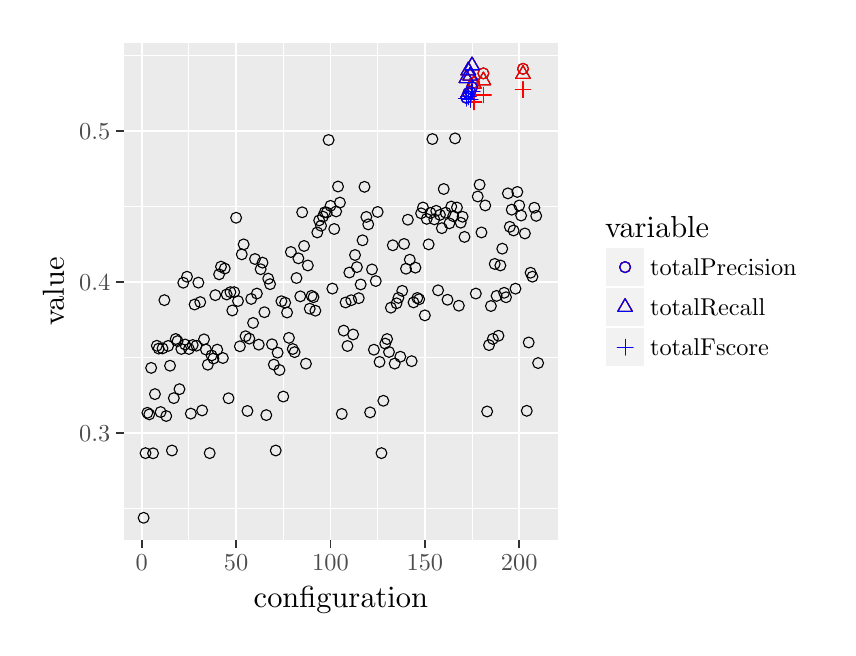
\begin{tikzpicture}[x=1pt,y=1pt]
\definecolor{fillColor}{RGB}{255,255,255}
\path[use as bounding box,fill=fillColor,fill opacity=0.00] (0,0) rectangle (289.08,216.81);
\begin{scope}
\path[clip] (  0.00,  0.00) rectangle (289.08,216.81);
\definecolor{drawColor}{RGB}{255,255,255}
\definecolor{fillColor}{RGB}{255,255,255}

\path[draw=drawColor,line width= 0.6pt,line join=round,line cap=round,fill=fillColor] (  0.00,  0.00) rectangle (289.08,216.81);
\end{scope}
\begin{scope}
\path[clip] ( 34.77, 31.53) rectangle (191.57,211.31);
\definecolor{fillColor}{gray}{0.92}

\path[fill=fillColor] ( 34.77, 31.53) rectangle (191.57,211.31);
\definecolor{drawColor}{RGB}{255,255,255}

\path[draw=drawColor,line width= 0.3pt,line join=round] ( 34.77, 43.14) --
	(191.57, 43.14);

\path[draw=drawColor,line width= 0.3pt,line join=round] ( 34.77, 97.66) --
	(191.57, 97.66);

\path[draw=drawColor,line width= 0.3pt,line join=round] ( 34.77,152.19) --
	(191.57,152.19);

\path[draw=drawColor,line width= 0.3pt,line join=round] ( 34.77,206.71) --
	(191.57,206.71);

\path[draw=drawColor,line width= 0.3pt,line join=round] ( 58.26, 31.53) --
	( 58.26,211.31);

\path[draw=drawColor,line width= 0.3pt,line join=round] ( 92.37, 31.53) --
	( 92.37,211.31);

\path[draw=drawColor,line width= 0.3pt,line join=round] (126.47, 31.53) --
	(126.47,211.31);

\path[draw=drawColor,line width= 0.3pt,line join=round] (160.57, 31.53) --
	(160.57,211.31);

\path[draw=drawColor,line width= 0.6pt,line join=round] ( 34.77, 70.40) --
	(191.57, 70.40);

\path[draw=drawColor,line width= 0.6pt,line join=round] ( 34.77,124.92) --
	(191.57,124.92);

\path[draw=drawColor,line width= 0.6pt,line join=round] ( 34.77,179.45) --
	(191.57,179.45);

\path[draw=drawColor,line width= 0.6pt,line join=round] ( 41.21, 31.53) --
	( 41.21,211.31);

\path[draw=drawColor,line width= 0.6pt,line join=round] ( 75.32, 31.53) --
	( 75.32,211.31);

\path[draw=drawColor,line width= 0.6pt,line join=round] (109.42, 31.53) --
	(109.42,211.31);

\path[draw=drawColor,line width= 0.6pt,line join=round] (143.52, 31.53) --
	(143.52,211.31);

\path[draw=drawColor,line width= 0.6pt,line join=round] (177.63, 31.53) --
	(177.63,211.31);
\definecolor{drawColor}{RGB}{0,0,0}

\path[draw=drawColor,line width= 0.4pt,line join=round,line cap=round] ( 41.90, 39.70) circle (  1.96);

\path[draw=drawColor,line width= 0.4pt,line join=round,line cap=round] ( 42.58, 63.07) circle (  1.96);

\path[draw=drawColor,line width= 0.4pt,line join=round,line cap=round] ( 43.26, 77.65) circle (  1.96);

\path[draw=drawColor,line width= 0.4pt,line join=round,line cap=round] ( 43.94, 77.08) circle (  1.96);

\path[draw=drawColor,line width= 0.4pt,line join=round,line cap=round] ( 44.62, 93.87) circle (  1.96);

\path[draw=drawColor,line width= 0.4pt,line join=round,line cap=round] ( 45.31, 63.01) circle (  1.96);

\path[draw=drawColor,line width= 0.4pt,line join=round,line cap=round] ( 45.99, 84.39) circle (  1.96);

\path[draw=drawColor,line width= 0.4pt,line join=round,line cap=round] ( 46.67,101.86) circle (  1.96);

\path[draw=drawColor,line width= 0.4pt,line join=round,line cap=round] ( 47.35,100.85) circle (  1.96);

\path[draw=drawColor,line width= 0.4pt,line join=round,line cap=round] ( 48.03, 77.92) circle (  1.96);

\path[draw=drawColor,line width= 0.4pt,line join=round,line cap=round] ( 48.72,100.91) circle (  1.96);

\path[draw=drawColor,line width= 0.4pt,line join=round,line cap=round] ( 49.40,118.35) circle (  1.96);

\path[draw=drawColor,line width= 0.4pt,line join=round,line cap=round] ( 50.08, 76.48) circle (  1.96);

\path[draw=drawColor,line width= 0.4pt,line join=round,line cap=round] ( 50.76,101.81) circle (  1.96);

\path[draw=drawColor,line width= 0.4pt,line join=round,line cap=round] ( 51.44, 94.66) circle (  1.96);

\path[draw=drawColor,line width= 0.4pt,line join=round,line cap=round] ( 52.13, 64.02) circle (  1.96);

\path[draw=drawColor,line width= 0.4pt,line join=round,line cap=round] ( 52.81, 82.94) circle (  1.96);

\path[draw=drawColor,line width= 0.4pt,line join=round,line cap=round] ( 53.49,104.31) circle (  1.96);

\path[draw=drawColor,line width= 0.4pt,line join=round,line cap=round] ( 54.17,103.55) circle (  1.96);

\path[draw=drawColor,line width= 0.4pt,line join=round,line cap=round] ( 54.85, 86.18) circle (  1.96);

\path[draw=drawColor,line width= 0.4pt,line join=round,line cap=round] ( 55.54,100.72) circle (  1.96);

\path[draw=drawColor,line width= 0.4pt,line join=round,line cap=round] ( 56.22,124.65) circle (  1.96);

\path[draw=drawColor,line width= 0.4pt,line join=round,line cap=round] ( 56.90,102.32) circle (  1.96);

\path[draw=drawColor,line width= 0.4pt,line join=round,line cap=round] ( 57.58,126.81) circle (  1.96);

\path[draw=drawColor,line width= 0.4pt,line join=round,line cap=round] ( 58.26,100.72) circle (  1.96);

\path[draw=drawColor,line width= 0.4pt,line join=round,line cap=round] ( 58.95, 77.35) circle (  1.96);

\path[draw=drawColor,line width= 0.4pt,line join=round,line cap=round] ( 59.63,102.13) circle (  1.96);

\path[draw=drawColor,line width= 0.4pt,line join=round,line cap=round] ( 60.31,116.77) circle (  1.96);

\path[draw=drawColor,line width= 0.4pt,line join=round,line cap=round] ( 60.99,101.89) circle (  1.96);

\path[draw=drawColor,line width= 0.4pt,line join=round,line cap=round] ( 61.68,124.68) circle (  1.96);

\path[draw=drawColor,line width= 0.4pt,line join=round,line cap=round] ( 62.36,117.65) circle (  1.96);

\path[draw=drawColor,line width= 0.4pt,line join=round,line cap=round] ( 63.04, 78.50) circle (  1.96);

\path[draw=drawColor,line width= 0.4pt,line join=round,line cap=round] ( 63.72,104.18) circle (  1.96);

\path[draw=drawColor,line width= 0.4pt,line join=round,line cap=round] ( 64.40,100.50) circle (  1.96);

\path[draw=drawColor,line width= 0.4pt,line join=round,line cap=round] ( 65.09, 95.02) circle (  1.96);

\path[draw=drawColor,line width= 0.4pt,line join=round,line cap=round] ( 65.77, 63.07) circle (  1.96);

\path[draw=drawColor,line width= 0.4pt,line join=round,line cap=round] ( 66.45, 98.37) circle (  1.96);

\path[draw=drawColor,line width= 0.4pt,line join=round,line cap=round] ( 67.13, 97.25) circle (  1.96);

\path[draw=drawColor,line width= 0.4pt,line join=round,line cap=round] ( 67.81,120.15) circle (  1.96);

\path[draw=drawColor,line width= 0.4pt,line join=round,line cap=round] ( 68.50,100.47) circle (  1.96);

\path[draw=drawColor,line width= 0.4pt,line join=round,line cap=round] ( 69.18,127.68) circle (  1.96);

\path[draw=drawColor,line width= 0.4pt,line join=round,line cap=round] ( 69.86,130.46) circle (  1.96);

\path[draw=drawColor,line width= 0.4pt,line join=round,line cap=round] ( 70.54, 97.44) circle (  1.96);

\path[draw=drawColor,line width= 0.4pt,line join=round,line cap=round] ( 71.22,129.78) circle (  1.96);

\path[draw=drawColor,line width= 0.4pt,line join=round,line cap=round] ( 71.91,120.40) circle (  1.96);

\path[draw=drawColor,line width= 0.4pt,line join=round,line cap=round] ( 72.59, 82.89) circle (  1.96);

\path[draw=drawColor,line width= 0.4pt,line join=round,line cap=round] ( 73.27,121.24) circle (  1.96);

\path[draw=drawColor,line width= 0.4pt,line join=round,line cap=round] ( 73.95,114.62) circle (  1.96);

\path[draw=drawColor,line width= 0.4pt,line join=round,line cap=round] ( 74.63,121.24) circle (  1.96);

\path[draw=drawColor,line width= 0.4pt,line join=round,line cap=round] ( 75.32,148.12) circle (  1.96);

\path[draw=drawColor,line width= 0.4pt,line join=round,line cap=round] ( 76.00,118.03) circle (  1.96);

\path[draw=drawColor,line width= 0.4pt,line join=round,line cap=round] ( 76.68,101.67) circle (  1.96);

\path[draw=drawColor,line width= 0.4pt,line join=round,line cap=round] ( 77.36,134.90) circle (  1.96);

\path[draw=drawColor,line width= 0.4pt,line join=round,line cap=round] ( 78.04,138.50) circle (  1.96);

\path[draw=drawColor,line width= 0.4pt,line join=round,line cap=round] ( 78.73,105.32) circle (  1.96);

\path[draw=drawColor,line width= 0.4pt,line join=round,line cap=round] ( 79.41, 78.31) circle (  1.96);

\path[draw=drawColor,line width= 0.4pt,line join=round,line cap=round] ( 80.09,104.45) circle (  1.96);

\path[draw=drawColor,line width= 0.4pt,line join=round,line cap=round] ( 80.77,118.79) circle (  1.96);

\path[draw=drawColor,line width= 0.4pt,line join=round,line cap=round] ( 81.45,110.12) circle (  1.96);

\path[draw=drawColor,line width= 0.4pt,line join=round,line cap=round] ( 82.14,133.21) circle (  1.96);

\path[draw=drawColor,line width= 0.4pt,line join=round,line cap=round] ( 82.82,120.73) circle (  1.96);

\path[draw=drawColor,line width= 0.4pt,line join=round,line cap=round] ( 83.50,102.27) circle (  1.96);

\path[draw=drawColor,line width= 0.4pt,line join=round,line cap=round] ( 84.18,129.53) circle (  1.96);

\path[draw=drawColor,line width= 0.4pt,line join=round,line cap=round] ( 84.87,131.90) circle (  1.96);

\path[draw=drawColor,line width= 0.4pt,line join=round,line cap=round] ( 85.55,113.99) circle (  1.96);

\path[draw=drawColor,line width= 0.4pt,line join=round,line cap=round] ( 86.23, 76.81) circle (  1.96);

\path[draw=drawColor,line width= 0.4pt,line join=round,line cap=round] ( 86.91,126.12) circle (  1.96);

\path[draw=drawColor,line width= 0.4pt,line join=round,line cap=round] ( 87.59,124.13) circle (  1.96);

\path[draw=drawColor,line width= 0.4pt,line join=round,line cap=round] ( 88.28,102.41) circle (  1.96);

\path[draw=drawColor,line width= 0.4pt,line join=round,line cap=round] ( 88.96, 95.07) circle (  1.96);

\path[draw=drawColor,line width= 0.4pt,line join=round,line cap=round] ( 89.64, 64.02) circle (  1.96);

\path[draw=drawColor,line width= 0.4pt,line join=round,line cap=round] ( 90.32, 99.38) circle (  1.96);

\path[draw=drawColor,line width= 0.4pt,line join=round,line cap=round] ( 91.00, 93.11) circle (  1.96);

\path[draw=drawColor,line width= 0.4pt,line join=round,line cap=round] ( 91.69,117.97) circle (  1.96);

\path[draw=drawColor,line width= 0.4pt,line join=round,line cap=round] ( 92.37, 83.51) circle (  1.96);

\path[draw=drawColor,line width= 0.4pt,line join=round,line cap=round] ( 93.05,117.43) circle (  1.96);

\path[draw=drawColor,line width= 0.4pt,line join=round,line cap=round] ( 93.73,113.88) circle (  1.96);

\path[draw=drawColor,line width= 0.4pt,line join=round,line cap=round] ( 94.41,104.72) circle (  1.96);

\path[draw=drawColor,line width= 0.4pt,line join=round,line cap=round] ( 95.10,135.75) circle (  1.96);

\path[draw=drawColor,line width= 0.4pt,line join=round,line cap=round] ( 95.78,100.69) circle (  1.96);

\path[draw=drawColor,line width= 0.4pt,line join=round,line cap=round] ( 96.46, 99.57) circle (  1.96);

\path[draw=drawColor,line width= 0.4pt,line join=round,line cap=round] ( 97.14,126.34) circle (  1.96);

\path[draw=drawColor,line width= 0.4pt,line join=round,line cap=round] ( 97.82,133.46) circle (  1.96);

\path[draw=drawColor,line width= 0.4pt,line join=round,line cap=round] ( 98.51,119.72) circle (  1.96);

\path[draw=drawColor,line width= 0.4pt,line join=round,line cap=round] ( 99.19,150.09) circle (  1.96);

\path[draw=drawColor,line width= 0.4pt,line join=round,line cap=round] ( 99.87,137.93) circle (  1.96);

\path[draw=drawColor,line width= 0.4pt,line join=round,line cap=round] (100.55, 95.40) circle (  1.96);

\path[draw=drawColor,line width= 0.4pt,line join=round,line cap=round] (101.23,130.89) circle (  1.96);

\path[draw=drawColor,line width= 0.4pt,line join=round,line cap=round] (101.92,115.27) circle (  1.96);

\path[draw=drawColor,line width= 0.4pt,line join=round,line cap=round] (102.60,119.91) circle (  1.96);

\path[draw=drawColor,line width= 0.4pt,line join=round,line cap=round] (103.28,119.42) circle (  1.96);

\path[draw=drawColor,line width= 0.4pt,line join=round,line cap=round] (103.96,114.54) circle (  1.96);

\path[draw=drawColor,line width= 0.4pt,line join=round,line cap=round] (104.65,142.81) circle (  1.96);

\path[draw=drawColor,line width= 0.4pt,line join=round,line cap=round] (105.33,147.17) circle (  1.96);

\path[draw=drawColor,line width= 0.4pt,line join=round,line cap=round] (106.01,145.23) circle (  1.96);

\path[draw=drawColor,line width= 0.4pt,line join=round,line cap=round] (106.69,148.53) circle (  1.96);

\path[draw=drawColor,line width= 0.4pt,line join=round,line cap=round] (107.37,150.11) circle (  1.96);

\path[draw=drawColor,line width= 0.4pt,line join=round,line cap=round] (108.06,150.03) circle (  1.96);

\path[draw=drawColor,line width= 0.4pt,line join=round,line cap=round] (108.74,176.23) circle (  1.96);

\path[draw=drawColor,line width= 0.4pt,line join=round,line cap=round] (109.42,152.43) circle (  1.96);

\path[draw=drawColor,line width= 0.4pt,line join=round,line cap=round] (110.10,122.53) circle (  1.96);

\path[draw=drawColor,line width= 0.4pt,line join=round,line cap=round] (110.78,144.06) circle (  1.96);

\path[draw=drawColor,line width= 0.4pt,line join=round,line cap=round] (111.47,150.41) circle (  1.96);

\path[draw=drawColor,line width= 0.4pt,line join=round,line cap=round] (112.15,159.41) circle (  1.96);

\path[draw=drawColor,line width= 0.4pt,line join=round,line cap=round] (112.83,153.60) circle (  1.96);

\path[draw=drawColor,line width= 0.4pt,line join=round,line cap=round] (113.51, 77.24) circle (  1.96);

\path[draw=drawColor,line width= 0.4pt,line join=round,line cap=round] (114.19,107.34) circle (  1.96);

\path[draw=drawColor,line width= 0.4pt,line join=round,line cap=round] (114.88,117.51) circle (  1.96);

\path[draw=drawColor,line width= 0.4pt,line join=round,line cap=round] (115.56,101.78) circle (  1.96);

\path[draw=drawColor,line width= 0.4pt,line join=round,line cap=round] (116.24,128.33) circle (  1.96);

\path[draw=drawColor,line width= 0.4pt,line join=round,line cap=round] (116.92,118.33) circle (  1.96);

\path[draw=drawColor,line width= 0.4pt,line join=round,line cap=round] (117.60,105.95) circle (  1.96);

\path[draw=drawColor,line width= 0.4pt,line join=round,line cap=round] (118.29,134.66) circle (  1.96);

\path[draw=drawColor,line width= 0.4pt,line join=round,line cap=round] (118.97,130.29) circle (  1.96);

\path[draw=drawColor,line width= 0.4pt,line join=round,line cap=round] (119.65,119.06) circle (  1.96);

\path[draw=drawColor,line width= 0.4pt,line join=round,line cap=round] (120.33,124.02) circle (  1.96);

\path[draw=drawColor,line width= 0.4pt,line join=round,line cap=round] (121.01,139.97) circle (  1.96);

\path[draw=drawColor,line width= 0.4pt,line join=round,line cap=round] (121.70,159.30) circle (  1.96);

\path[draw=drawColor,line width= 0.4pt,line join=round,line cap=round] (122.38,148.42) circle (  1.96);

\path[draw=drawColor,line width= 0.4pt,line join=round,line cap=round] (123.06,145.73) circle (  1.96);

\path[draw=drawColor,line width= 0.4pt,line join=round,line cap=round] (123.74, 77.79) circle (  1.96);

\path[draw=drawColor,line width= 0.4pt,line join=round,line cap=round] (124.42,129.45) circle (  1.96);

\path[draw=drawColor,line width= 0.4pt,line join=round,line cap=round] (125.11,100.44) circle (  1.96);

\path[draw=drawColor,line width= 0.4pt,line join=round,line cap=round] (125.79,125.25) circle (  1.96);

\path[draw=drawColor,line width= 0.4pt,line join=round,line cap=round] (126.47,150.22) circle (  1.96);

\path[draw=drawColor,line width= 0.4pt,line join=round,line cap=round] (127.15, 96.03) circle (  1.96);

\path[draw=drawColor,line width= 0.4pt,line join=round,line cap=round] (127.84, 63.07) circle (  1.96);

\path[draw=drawColor,line width= 0.4pt,line join=round,line cap=round] (128.52, 81.99) circle (  1.96);

\path[draw=drawColor,line width= 0.4pt,line join=round,line cap=round] (129.20,102.65) circle (  1.96);

\path[draw=drawColor,line width= 0.4pt,line join=round,line cap=round] (129.88,104.29) circle (  1.96);

\path[draw=drawColor,line width= 0.4pt,line join=round,line cap=round] (130.56, 99.62) circle (  1.96);

\path[draw=drawColor,line width= 0.4pt,line join=round,line cap=round] (131.25,115.63) circle (  1.96);

\path[draw=drawColor,line width= 0.4pt,line join=round,line cap=round] (131.93,138.17) circle (  1.96);

\path[draw=drawColor,line width= 0.4pt,line join=round,line cap=round] (132.61, 95.43) circle (  1.96);

\path[draw=drawColor,line width= 0.4pt,line join=round,line cap=round] (133.29,117.21) circle (  1.96);

\path[draw=drawColor,line width= 0.4pt,line join=round,line cap=round] (133.97,119.17) circle (  1.96);

\path[draw=drawColor,line width= 0.4pt,line join=round,line cap=round] (134.66, 97.91) circle (  1.96);

\path[draw=drawColor,line width= 0.4pt,line join=round,line cap=round] (135.34,121.71) circle (  1.96);

\path[draw=drawColor,line width= 0.4pt,line join=round,line cap=round] (136.02,138.66) circle (  1.96);

\path[draw=drawColor,line width= 0.4pt,line join=round,line cap=round] (136.70,129.70) circle (  1.96);

\path[draw=drawColor,line width= 0.4pt,line join=round,line cap=round] (137.38,147.42) circle (  1.96);

\path[draw=drawColor,line width= 0.4pt,line join=round,line cap=round] (138.07,132.97) circle (  1.96);

\path[draw=drawColor,line width= 0.4pt,line join=round,line cap=round] (138.75, 96.30) circle (  1.96);

\path[draw=drawColor,line width= 0.4pt,line join=round,line cap=round] (139.43,117.54) circle (  1.96);

\path[draw=drawColor,line width= 0.4pt,line join=round,line cap=round] (140.11,130.10) circle (  1.96);

\path[draw=drawColor,line width= 0.4pt,line join=round,line cap=round] (140.79,119.14) circle (  1.96);

\path[draw=drawColor,line width= 0.4pt,line join=round,line cap=round] (141.48,118.68) circle (  1.96);

\path[draw=drawColor,line width= 0.4pt,line join=round,line cap=round] (142.16,149.73) circle (  1.96);

\path[draw=drawColor,line width= 0.4pt,line join=round,line cap=round] (142.84,151.83) circle (  1.96);

\path[draw=drawColor,line width= 0.4pt,line join=round,line cap=round] (143.52,112.85) circle (  1.96);

\path[draw=drawColor,line width= 0.4pt,line join=round,line cap=round] (144.20,147.72) circle (  1.96);

\path[draw=drawColor,line width= 0.4pt,line join=round,line cap=round] (144.89,138.50) circle (  1.96);

\path[draw=drawColor,line width= 0.4pt,line join=round,line cap=round] (145.57,149.87) circle (  1.96);

\path[draw=drawColor,line width= 0.4pt,line join=round,line cap=round] (146.25,176.56) circle (  1.96);

\path[draw=drawColor,line width= 0.4pt,line join=round,line cap=round] (146.93,147.55) circle (  1.96);

\path[draw=drawColor,line width= 0.4pt,line join=round,line cap=round] (147.62,150.63) circle (  1.96);

\path[draw=drawColor,line width= 0.4pt,line join=round,line cap=round] (148.30,121.90) circle (  1.96);

\path[draw=drawColor,line width= 0.4pt,line join=round,line cap=round] (148.98,149.16) circle (  1.96);

\path[draw=drawColor,line width= 0.4pt,line join=round,line cap=round] (149.66,144.36) circle (  1.96);

\path[draw=drawColor,line width= 0.4pt,line join=round,line cap=round] (150.34,158.51) circle (  1.96);

\path[draw=drawColor,line width= 0.4pt,line join=round,line cap=round] (151.03,149.95) circle (  1.96);

\path[draw=drawColor,line width= 0.4pt,line join=round,line cap=round] (151.71,118.49) circle (  1.96);

\path[draw=drawColor,line width= 0.4pt,line join=round,line cap=round] (152.39,146.11) circle (  1.96);

\path[draw=drawColor,line width= 0.4pt,line join=round,line cap=round] (153.07,152.16) circle (  1.96);

\path[draw=drawColor,line width= 0.4pt,line join=round,line cap=round] (153.75,148.72) circle (  1.96);

\path[draw=drawColor,line width= 0.4pt,line join=round,line cap=round] (154.44,176.80) circle (  1.96);

\path[draw=drawColor,line width= 0.4pt,line join=round,line cap=round] (155.12,151.83) circle (  1.96);

\path[draw=drawColor,line width= 0.4pt,line join=round,line cap=round] (155.80,116.34) circle (  1.96);

\path[draw=drawColor,line width= 0.4pt,line join=round,line cap=round] (156.48,146.33) circle (  1.96);

\path[draw=drawColor,line width= 0.4pt,line join=round,line cap=round] (157.16,148.48) circle (  1.96);

\path[draw=drawColor,line width= 0.4pt,line join=round,line cap=round] (157.85,141.20) circle (  1.96);

\path[draw=drawColor,line width= 0.4pt,line join=round,line cap=round] (158.53,191.47) circle (  1.96);

\path[draw=drawColor,line width= 0.4pt,line join=round,line cap=round] (159.21,193.13) circle (  1.96);

\path[draw=drawColor,line width= 0.4pt,line join=round,line cap=round] (159.89,193.63) circle (  1.96);

\path[draw=drawColor,line width= 0.4pt,line join=round,line cap=round] (160.57,195.34) circle (  1.96);

\path[draw=drawColor,line width= 0.4pt,line join=round,line cap=round] (161.26,196.98) circle (  1.96);

\path[draw=drawColor,line width= 0.4pt,line join=round,line cap=round] (161.94,120.73) circle (  1.96);

\path[draw=drawColor,line width= 0.4pt,line join=round,line cap=round] (162.62,155.81) circle (  1.96);

\path[draw=drawColor,line width= 0.4pt,line join=round,line cap=round] (163.30,160.07) circle (  1.96);

\path[draw=drawColor,line width= 0.4pt,line join=round,line cap=round] (163.98,142.81) circle (  1.96);

\path[draw=drawColor,line width= 0.4pt,line join=round,line cap=round] (164.67,200.30) circle (  1.96);

\path[draw=drawColor,line width= 0.4pt,line join=round,line cap=round] (165.35,152.57) circle (  1.96);

\path[draw=drawColor,line width= 0.4pt,line join=round,line cap=round] (166.03, 78.12) circle (  1.96);

\path[draw=drawColor,line width= 0.4pt,line join=round,line cap=round] (166.71,102.11) circle (  1.96);

\path[draw=drawColor,line width= 0.4pt,line join=round,line cap=round] (167.39,116.23) circle (  1.96);

\path[draw=drawColor,line width= 0.4pt,line join=round,line cap=round] (168.08,104.34) circle (  1.96);

\path[draw=drawColor,line width= 0.4pt,line join=round,line cap=round] (168.76,131.44) circle (  1.96);

\path[draw=drawColor,line width= 0.4pt,line join=round,line cap=round] (169.44,119.88) circle (  1.96);

\path[draw=drawColor,line width= 0.4pt,line join=round,line cap=round] (170.12,105.49) circle (  1.96);

\path[draw=drawColor,line width= 0.4pt,line join=round,line cap=round] (170.81,130.89) circle (  1.96);

\path[draw=drawColor,line width= 0.4pt,line join=round,line cap=round] (171.49,136.95) circle (  1.96);

\path[draw=drawColor,line width= 0.4pt,line join=round,line cap=round] (172.17,121.00) circle (  1.96);

\path[draw=drawColor,line width= 0.4pt,line join=round,line cap=round] (172.85,119.39) circle (  1.96);

\path[draw=drawColor,line width= 0.4pt,line join=round,line cap=round] (173.53,156.93) circle (  1.96);

\path[draw=drawColor,line width= 0.4pt,line join=round,line cap=round] (174.22,144.85) circle (  1.96);

\path[draw=drawColor,line width= 0.4pt,line join=round,line cap=round] (174.90,151.04) circle (  1.96);

\path[draw=drawColor,line width= 0.4pt,line join=round,line cap=round] (175.58,143.52) circle (  1.96);

\path[draw=drawColor,line width= 0.4pt,line join=round,line cap=round] (176.26,122.50) circle (  1.96);

\path[draw=drawColor,line width= 0.4pt,line join=round,line cap=round] (176.94,157.45) circle (  1.96);

\path[draw=drawColor,line width= 0.4pt,line join=round,line cap=round] (177.63,152.57) circle (  1.96);

\path[draw=drawColor,line width= 0.4pt,line join=round,line cap=round] (178.31,148.92) circle (  1.96);

\path[draw=drawColor,line width= 0.4pt,line join=round,line cap=round] (178.99,201.94) circle (  1.96);

\path[draw=drawColor,line width= 0.4pt,line join=round,line cap=round] (179.67,142.45) circle (  1.96);

\path[draw=drawColor,line width= 0.4pt,line join=round,line cap=round] (180.35, 78.36) circle (  1.96);

\path[draw=drawColor,line width= 0.4pt,line join=round,line cap=round] (181.04,103.06) circle (  1.96);

\path[draw=drawColor,line width= 0.4pt,line join=round,line cap=round] (181.72,128.25) circle (  1.96);

\path[draw=drawColor,line width= 0.4pt,line join=round,line cap=round] (182.40,126.83) circle (  1.96);

\path[draw=drawColor,line width= 0.4pt,line join=round,line cap=round] (183.08,151.75) circle (  1.96);

\path[draw=drawColor,line width= 0.4pt,line join=round,line cap=round] (183.76,148.81) circle (  1.96);

\path[draw=drawColor,line width= 0.4pt,line join=round,line cap=round] (184.45, 95.62) circle (  1.96);

\path[draw=drawColor,line width= 0.4pt,line join=round,line cap=round] (158.53,201.52) --
	(161.17,196.95) --
	(155.89,196.95) --
	(158.53,201.52);

\path[draw=drawColor,line width= 0.4pt,line join=round,line cap=round] (159.21,204.34) --
	(161.85,199.76) --
	(156.57,199.76) --
	(159.21,204.34);

\path[draw=drawColor,line width= 0.4pt,line join=round,line cap=round] (159.89,202.43) --
	(162.53,197.86) --
	(157.25,197.86) --
	(159.89,202.43);

\path[draw=drawColor,line width= 0.4pt,line join=round,line cap=round] (160.57,206.19) --
	(163.22,201.61) --
	(157.93,201.61) --
	(160.57,206.19);

\path[draw=drawColor,line width= 0.4pt,line join=round,line cap=round] (161.26,199.50) --
	(163.90,194.92) --
	(158.61,194.92) --
	(161.26,199.50);

\path[draw=drawColor,line width= 0.4pt,line join=round,line cap=round] (164.67,200.77) --
	(167.31,196.19) --
	(162.02,196.19) --
	(164.67,200.77);

\path[draw=drawColor,line width= 0.4pt,line join=round,line cap=round] (178.99,203.07) --
	(181.63,198.49) --
	(176.35,198.49) --
	(178.99,203.07);

\path[draw=drawColor,line width= 0.4pt,line join=round,line cap=round] (155.75,191.33) -- (161.30,191.33);

\path[draw=drawColor,line width= 0.4pt,line join=round,line cap=round] (158.53,188.56) -- (158.53,194.11);

\path[draw=drawColor,line width= 0.4pt,line join=round,line cap=round] (156.44,191.80) -- (161.99,191.80);

\path[draw=drawColor,line width= 0.4pt,line join=round,line cap=round] (159.21,189.02) -- (159.21,194.57);

\path[draw=drawColor,line width= 0.4pt,line join=round,line cap=round] (157.12,190.90) -- (162.67,190.90);

\path[draw=drawColor,line width= 0.4pt,line join=round,line cap=round] (159.89,188.13) -- (159.89,193.68);

\path[draw=drawColor,line width= 0.4pt,line join=round,line cap=round] (157.80,193.70) -- (163.35,193.70);

\path[draw=drawColor,line width= 0.4pt,line join=round,line cap=round] (160.57,190.93) -- (160.57,196.48);

\path[draw=drawColor,line width= 0.4pt,line join=round,line cap=round] (158.48,189.95) -- (164.03,189.95);

\path[draw=drawColor,line width= 0.4pt,line join=round,line cap=round] (161.26,187.17) -- (161.26,192.72);

\path[draw=drawColor,line width= 0.4pt,line join=round,line cap=round] (161.89,192.49) -- (167.44,192.49);

\path[draw=drawColor,line width= 0.4pt,line join=round,line cap=round] (164.67,189.71) -- (164.67,195.26);

\path[draw=drawColor,line width= 0.4pt,line join=round,line cap=round] (176.22,194.45) -- (181.76,194.45);

\path[draw=drawColor,line width= 0.4pt,line join=round,line cap=round] (178.99,191.67) -- (178.99,197.22);
\definecolor{drawColor}{RGB}{255,0,0}

\path[draw=drawColor,line width= 0.4pt,line join=round,line cap=round] (158.53,191.47) circle (  1.96);

\path[draw=drawColor,line width= 0.4pt,line join=round,line cap=round] (159.21,193.13) circle (  1.96);

\path[draw=drawColor,line width= 0.4pt,line join=round,line cap=round] (159.89,193.63) circle (  1.96);

\path[draw=drawColor,line width= 0.4pt,line join=round,line cap=round] (160.57,195.34) circle (  1.96);

\path[draw=drawColor,line width= 0.4pt,line join=round,line cap=round] (161.26,196.98) circle (  1.96);

\path[draw=drawColor,line width= 0.4pt,line join=round,line cap=round] (164.67,200.30) circle (  1.96);

\path[draw=drawColor,line width= 0.4pt,line join=round,line cap=round] (178.99,201.94) circle (  1.96);

\path[draw=drawColor,line width= 0.4pt,line join=round,line cap=round] (158.53,201.52) --
	(161.17,196.95) --
	(155.89,196.95) --
	(158.53,201.52);

\path[draw=drawColor,line width= 0.4pt,line join=round,line cap=round] (159.21,204.34) --
	(161.85,199.76) --
	(156.57,199.76) --
	(159.21,204.34);

\path[draw=drawColor,line width= 0.4pt,line join=round,line cap=round] (159.89,202.43) --
	(162.53,197.86) --
	(157.25,197.86) --
	(159.89,202.43);

\path[draw=drawColor,line width= 0.4pt,line join=round,line cap=round] (160.57,206.19) --
	(163.22,201.61) --
	(157.93,201.61) --
	(160.57,206.19);

\path[draw=drawColor,line width= 0.4pt,line join=round,line cap=round] (161.26,199.50) --
	(163.90,194.92) --
	(158.61,194.92) --
	(161.26,199.50);

\path[draw=drawColor,line width= 0.4pt,line join=round,line cap=round] (164.67,200.77) --
	(167.31,196.19) --
	(162.02,196.19) --
	(164.67,200.77);

\path[draw=drawColor,line width= 0.4pt,line join=round,line cap=round] (178.99,203.07) --
	(181.63,198.49) --
	(176.35,198.49) --
	(178.99,203.07);

\path[draw=drawColor,line width= 0.4pt,line join=round,line cap=round] (155.75,191.33) -- (161.30,191.33);

\path[draw=drawColor,line width= 0.4pt,line join=round,line cap=round] (158.53,188.56) -- (158.53,194.11);

\path[draw=drawColor,line width= 0.4pt,line join=round,line cap=round] (156.44,191.80) -- (161.99,191.80);

\path[draw=drawColor,line width= 0.4pt,line join=round,line cap=round] (159.21,189.02) -- (159.21,194.57);

\path[draw=drawColor,line width= 0.4pt,line join=round,line cap=round] (157.12,190.90) -- (162.67,190.90);

\path[draw=drawColor,line width= 0.4pt,line join=round,line cap=round] (159.89,188.13) -- (159.89,193.68);

\path[draw=drawColor,line width= 0.4pt,line join=round,line cap=round] (157.80,193.70) -- (163.35,193.70);

\path[draw=drawColor,line width= 0.4pt,line join=round,line cap=round] (160.57,190.93) -- (160.57,196.48);

\path[draw=drawColor,line width= 0.4pt,line join=round,line cap=round] (158.48,189.95) -- (164.03,189.95);

\path[draw=drawColor,line width= 0.4pt,line join=round,line cap=round] (161.26,187.17) -- (161.26,192.72);

\path[draw=drawColor,line width= 0.4pt,line join=round,line cap=round] (161.89,192.49) -- (167.44,192.49);

\path[draw=drawColor,line width= 0.4pt,line join=round,line cap=round] (164.67,189.71) -- (164.67,195.26);

\path[draw=drawColor,line width= 0.4pt,line join=round,line cap=round] (176.22,194.45) -- (181.76,194.45);

\path[draw=drawColor,line width= 0.4pt,line join=round,line cap=round] (178.99,191.67) -- (178.99,197.22);
\definecolor{drawColor}{RGB}{0,0,255}

\path[draw=drawColor,line width= 0.4pt,line join=round,line cap=round] (158.53,191.47) circle (  1.96);

\path[draw=drawColor,line width= 0.4pt,line join=round,line cap=round] (159.21,193.13) circle (  1.96);

\path[draw=drawColor,line width= 0.4pt,line join=round,line cap=round] (159.89,193.63) circle (  1.96);

\path[draw=drawColor,line width= 0.4pt,line join=round,line cap=round] (160.57,195.34) circle (  1.96);

\path[draw=drawColor,line width= 0.4pt,line join=round,line cap=round] (158.53,201.52) --
	(161.17,196.95) --
	(155.89,196.95) --
	(158.53,201.52);

\path[draw=drawColor,line width= 0.4pt,line join=round,line cap=round] (159.21,204.34) --
	(161.85,199.76) --
	(156.57,199.76) --
	(159.21,204.34);

\path[draw=drawColor,line width= 0.4pt,line join=round,line cap=round] (159.89,202.43) --
	(162.53,197.86) --
	(157.25,197.86) --
	(159.89,202.43);

\path[draw=drawColor,line width= 0.4pt,line join=round,line cap=round] (160.57,206.19) --
	(163.22,201.61) --
	(157.93,201.61) --
	(160.57,206.19);

\path[draw=drawColor,line width= 0.4pt,line join=round,line cap=round] (155.75,191.33) -- (161.30,191.33);

\path[draw=drawColor,line width= 0.4pt,line join=round,line cap=round] (158.53,188.56) -- (158.53,194.11);

\path[draw=drawColor,line width= 0.4pt,line join=round,line cap=round] (156.44,191.80) -- (161.99,191.80);

\path[draw=drawColor,line width= 0.4pt,line join=round,line cap=round] (159.21,189.02) -- (159.21,194.57);

\path[draw=drawColor,line width= 0.4pt,line join=round,line cap=round] (157.12,190.90) -- (162.67,190.90);

\path[draw=drawColor,line width= 0.4pt,line join=round,line cap=round] (159.89,188.13) -- (159.89,193.68);

\path[draw=drawColor,line width= 0.4pt,line join=round,line cap=round] (157.80,193.70) -- (163.35,193.70);

\path[draw=drawColor,line width= 0.4pt,line join=round,line cap=round] (160.57,190.93) -- (160.57,196.48);
\end{scope}
\begin{scope}
\path[clip] (  0.00,  0.00) rectangle (289.08,216.81);
\definecolor{drawColor}{gray}{0.30}

\node[text=drawColor,anchor=base east,inner sep=0pt, outer sep=0pt, scale=  0.88] at ( 29.82, 67.37) {0.3};

\node[text=drawColor,anchor=base east,inner sep=0pt, outer sep=0pt, scale=  0.88] at ( 29.82,121.89) {0.4};

\node[text=drawColor,anchor=base east,inner sep=0pt, outer sep=0pt, scale=  0.88] at ( 29.82,176.42) {0.5};
\end{scope}
\begin{scope}
\path[clip] (  0.00,  0.00) rectangle (289.08,216.81);
\definecolor{drawColor}{gray}{0.20}

\path[draw=drawColor,line width= 0.6pt,line join=round] ( 32.02, 70.40) --
	( 34.77, 70.40);

\path[draw=drawColor,line width= 0.6pt,line join=round] ( 32.02,124.92) --
	( 34.77,124.92);

\path[draw=drawColor,line width= 0.6pt,line join=round] ( 32.02,179.45) --
	( 34.77,179.45);
\end{scope}
\begin{scope}
\path[clip] (  0.00,  0.00) rectangle (289.08,216.81);
\definecolor{drawColor}{gray}{0.20}

\path[draw=drawColor,line width= 0.6pt,line join=round] ( 41.21, 28.78) --
	( 41.21, 31.53);

\path[draw=drawColor,line width= 0.6pt,line join=round] ( 75.32, 28.78) --
	( 75.32, 31.53);

\path[draw=drawColor,line width= 0.6pt,line join=round] (109.42, 28.78) --
	(109.42, 31.53);

\path[draw=drawColor,line width= 0.6pt,line join=round] (143.52, 28.78) --
	(143.52, 31.53);

\path[draw=drawColor,line width= 0.6pt,line join=round] (177.63, 28.78) --
	(177.63, 31.53);
\end{scope}
\begin{scope}
\path[clip] (  0.00,  0.00) rectangle (289.08,216.81);
\definecolor{drawColor}{gray}{0.30}

\node[text=drawColor,anchor=base,inner sep=0pt, outer sep=0pt, scale=  0.88] at ( 41.21, 20.52) {0};

\node[text=drawColor,anchor=base,inner sep=0pt, outer sep=0pt, scale=  0.88] at ( 75.32, 20.52) {50};

\node[text=drawColor,anchor=base,inner sep=0pt, outer sep=0pt, scale=  0.88] at (109.42, 20.52) {100};

\node[text=drawColor,anchor=base,inner sep=0pt, outer sep=0pt, scale=  0.88] at (143.52, 20.52) {150};

\node[text=drawColor,anchor=base,inner sep=0pt, outer sep=0pt, scale=  0.88] at (177.63, 20.52) {200};
\end{scope}
\begin{scope}
\path[clip] (  0.00,  0.00) rectangle (289.08,216.81);
\definecolor{drawColor}{RGB}{0,0,0}

\node[text=drawColor,anchor=base,inner sep=0pt, outer sep=0pt, scale=  1.10] at (113.17,  7.44) {configuration};
\end{scope}
\begin{scope}
\path[clip] (  0.00,  0.00) rectangle (289.08,216.81);
\definecolor{drawColor}{RGB}{0,0,0}

\node[text=drawColor,rotate= 90.00,anchor=base,inner sep=0pt, outer sep=0pt, scale=  1.10] at ( 13.08,121.42) {value};
\end{scope}
\begin{scope}
\path[clip] (  0.00,  0.00) rectangle (289.08,216.81);
\definecolor{fillColor}{RGB}{255,255,255}

\path[fill=fillColor] (202.96, 88.45) rectangle (283.58,154.39);
\end{scope}
\begin{scope}
\path[clip] (  0.00,  0.00) rectangle (289.08,216.81);
\definecolor{drawColor}{RGB}{0,0,0}

\node[text=drawColor,anchor=base west,inner sep=0pt, outer sep=0pt, scale=  1.10] at (208.65,141.12) {variable};
\end{scope}
\begin{scope}
\path[clip] (  0.00,  0.00) rectangle (289.08,216.81);
\definecolor{drawColor}{RGB}{255,255,255}
\definecolor{fillColor}{gray}{0.95}

\path[draw=drawColor,line width= 0.6pt,line join=round,line cap=round,fill=fillColor] (208.65,123.05) rectangle (223.10,137.51);
\end{scope}
\begin{scope}
\path[clip] (  0.00,  0.00) rectangle (289.08,216.81);
\definecolor{drawColor}{RGB}{0,0,0}

\path[draw=drawColor,line width= 0.4pt,line join=round,line cap=round] (215.87,130.28) circle (  1.96);
\end{scope}
\begin{scope}
\path[clip] (  0.00,  0.00) rectangle (289.08,216.81);
\definecolor{drawColor}{RGB}{255,0,0}

\path[draw=drawColor,line width= 0.4pt,line join=round,line cap=round] (215.87,130.28) circle (  1.96);
\end{scope}
\begin{scope}
\path[clip] (  0.00,  0.00) rectangle (289.08,216.81);
\definecolor{drawColor}{RGB}{0,0,255}

\path[draw=drawColor,line width= 0.4pt,line join=round,line cap=round] (215.87,130.28) circle (  1.96);
\end{scope}
\begin{scope}
\path[clip] (  0.00,  0.00) rectangle (289.08,216.81);
\definecolor{drawColor}{RGB}{255,255,255}
\definecolor{fillColor}{gray}{0.95}

\path[draw=drawColor,line width= 0.6pt,line join=round,line cap=round,fill=fillColor] (208.65,108.60) rectangle (223.10,123.05);
\end{scope}
\begin{scope}
\path[clip] (  0.00,  0.00) rectangle (289.08,216.81);
\definecolor{drawColor}{RGB}{0,0,0}

\path[draw=drawColor,line width= 0.4pt,line join=round,line cap=round] (215.87,118.88) --
	(218.52,114.30) --
	(213.23,114.30) --
	(215.87,118.88);
\end{scope}
\begin{scope}
\path[clip] (  0.00,  0.00) rectangle (289.08,216.81);
\definecolor{drawColor}{RGB}{255,0,0}

\path[draw=drawColor,line width= 0.4pt,line join=round,line cap=round] (215.87,118.88) --
	(218.52,114.30) --
	(213.23,114.30) --
	(215.87,118.88);
\end{scope}
\begin{scope}
\path[clip] (  0.00,  0.00) rectangle (289.08,216.81);
\definecolor{drawColor}{RGB}{0,0,255}

\path[draw=drawColor,line width= 0.4pt,line join=round,line cap=round] (215.87,118.88) --
	(218.52,114.30) --
	(213.23,114.30) --
	(215.87,118.88);
\end{scope}
\begin{scope}
\path[clip] (  0.00,  0.00) rectangle (289.08,216.81);
\definecolor{drawColor}{RGB}{255,255,255}
\definecolor{fillColor}{gray}{0.95}

\path[draw=drawColor,line width= 0.6pt,line join=round,line cap=round,fill=fillColor] (208.65, 94.14) rectangle (223.10,108.60);
\end{scope}
\begin{scope}
\path[clip] (  0.00,  0.00) rectangle (289.08,216.81);
\definecolor{drawColor}{RGB}{0,0,0}

\path[draw=drawColor,line width= 0.4pt,line join=round,line cap=round] (213.10,101.37) -- (218.65,101.37);

\path[draw=drawColor,line width= 0.4pt,line join=round,line cap=round] (215.87, 98.60) -- (215.87,104.15);
\end{scope}
\begin{scope}
\path[clip] (  0.00,  0.00) rectangle (289.08,216.81);
\definecolor{drawColor}{RGB}{255,0,0}

\path[draw=drawColor,line width= 0.4pt,line join=round,line cap=round] (213.10,101.37) -- (218.65,101.37);

\path[draw=drawColor,line width= 0.4pt,line join=round,line cap=round] (215.87, 98.60) -- (215.87,104.15);
\end{scope}
\begin{scope}
\path[clip] (  0.00,  0.00) rectangle (289.08,216.81);
\definecolor{drawColor}{RGB}{0,0,255}

\path[draw=drawColor,line width= 0.4pt,line join=round,line cap=round] (213.10,101.37) -- (218.65,101.37);

\path[draw=drawColor,line width= 0.4pt,line join=round,line cap=round] (215.87, 98.60) -- (215.87,104.15);
\end{scope}
\begin{scope}
\path[clip] (  0.00,  0.00) rectangle (289.08,216.81);
\definecolor{drawColor}{RGB}{0,0,0}

\node[text=drawColor,anchor=base west,inner sep=0pt, outer sep=0pt, scale=  0.88] at (224.91,127.25) {totalPrecision};
\end{scope}
\begin{scope}
\path[clip] (  0.00,  0.00) rectangle (289.08,216.81);
\definecolor{drawColor}{RGB}{0,0,0}

\node[text=drawColor,anchor=base west,inner sep=0pt, outer sep=0pt, scale=  0.88] at (224.91,112.80) {totalRecall};
\end{scope}
\begin{scope}
\path[clip] (  0.00,  0.00) rectangle (289.08,216.81);
\definecolor{drawColor}{RGB}{0,0,0}

\node[text=drawColor,anchor=base west,inner sep=0pt, outer sep=0pt, scale=  0.88] at (224.91, 98.34) {totalFscore};
\end{scope}
\end{tikzpicture}

  \end{center}
  \caption{Total measures on slip=guess=0.2, J=4}  
  \label{fig:theta02J4test}
\end{figure}

\begin{figure}[h!]
  \begin{center}
  % Created by tikzDevice version 0.10.1.2 on 2018-03-05 18:50:58
% !TEX encoding = UTF-8 Unicode
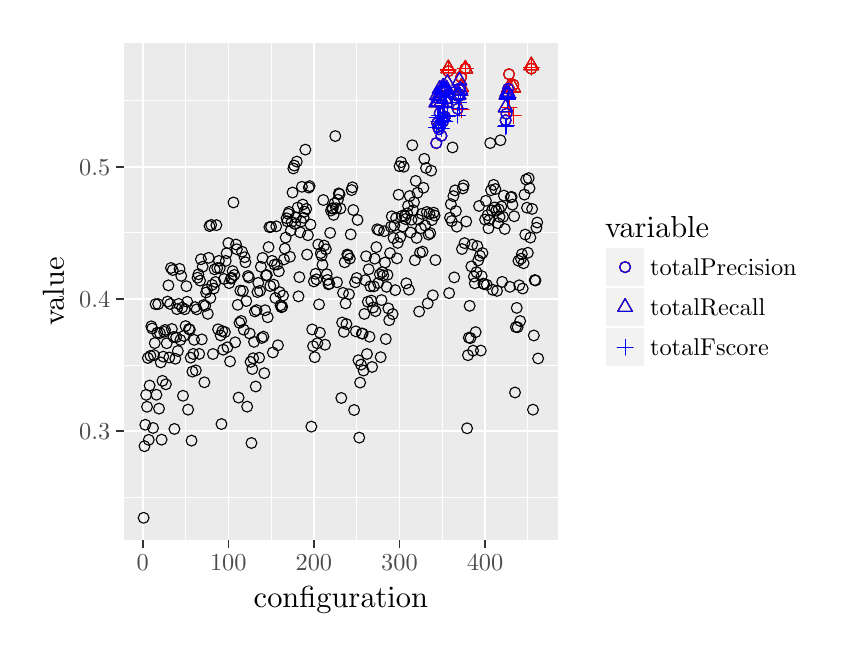
\begin{tikzpicture}[x=1pt,y=1pt]
\definecolor{fillColor}{RGB}{255,255,255}
\path[use as bounding box,fill=fillColor,fill opacity=0.00] (0,0) rectangle (289.08,216.81);
\begin{scope}
\path[clip] (  0.00,  0.00) rectangle (289.08,216.81);
\definecolor{drawColor}{RGB}{255,255,255}
\definecolor{fillColor}{RGB}{255,255,255}

\path[draw=drawColor,line width= 0.6pt,line join=round,line cap=round,fill=fillColor] (  0.00,  0.00) rectangle (289.08,216.81);
\end{scope}
\begin{scope}
\path[clip] ( 34.77, 31.53) rectangle (191.57,211.31);
\definecolor{fillColor}{gray}{0.92}

\path[fill=fillColor] ( 34.77, 31.53) rectangle (191.57,211.31);
\definecolor{drawColor}{RGB}{255,255,255}

\path[draw=drawColor,line width= 0.3pt,line join=round] ( 34.77, 47.11) --
	(191.57, 47.11);

\path[draw=drawColor,line width= 0.3pt,line join=round] ( 34.77, 94.90) --
	(191.57, 94.90);

\path[draw=drawColor,line width= 0.3pt,line join=round] ( 34.77,142.68) --
	(191.57,142.68);

\path[draw=drawColor,line width= 0.3pt,line join=round] ( 34.77,190.47) --
	(191.57,190.47);

\path[draw=drawColor,line width= 0.3pt,line join=round] ( 57.05, 31.53) --
	( 57.05,211.31);

\path[draw=drawColor,line width= 0.3pt,line join=round] ( 87.97, 31.53) --
	( 87.97,211.31);

\path[draw=drawColor,line width= 0.3pt,line join=round] (118.89, 31.53) --
	(118.89,211.31);

\path[draw=drawColor,line width= 0.3pt,line join=round] (149.81, 31.53) --
	(149.81,211.31);

\path[draw=drawColor,line width= 0.3pt,line join=round] (180.74, 31.53) --
	(180.74,211.31);

\path[draw=drawColor,line width= 0.6pt,line join=round] ( 34.77, 71.00) --
	(191.57, 71.00);

\path[draw=drawColor,line width= 0.6pt,line join=round] ( 34.77,118.79) --
	(191.57,118.79);

\path[draw=drawColor,line width= 0.6pt,line join=round] ( 34.77,166.58) --
	(191.57,166.58);

\path[draw=drawColor,line width= 0.6pt,line join=round] ( 41.59, 31.53) --
	( 41.59,211.31);

\path[draw=drawColor,line width= 0.6pt,line join=round] ( 72.51, 31.53) --
	( 72.51,211.31);

\path[draw=drawColor,line width= 0.6pt,line join=round] (103.43, 31.53) --
	(103.43,211.31);

\path[draw=drawColor,line width= 0.6pt,line join=round] (134.35, 31.53) --
	(134.35,211.31);

\path[draw=drawColor,line width= 0.6pt,line join=round] (165.27, 31.53) --
	(165.27,211.31);
\definecolor{drawColor}{RGB}{0,0,0}

\path[draw=drawColor,line width= 0.4pt,line join=round,line cap=round] ( 41.90, 39.70) circle (  1.96);

\path[draw=drawColor,line width= 0.4pt,line join=round,line cap=round] ( 42.20, 65.58) circle (  1.96);

\path[draw=drawColor,line width= 0.4pt,line join=round,line cap=round] ( 42.51, 73.32) circle (  1.96);

\path[draw=drawColor,line width= 0.4pt,line join=round,line cap=round] ( 42.82, 84.14) circle (  1.96);

\path[draw=drawColor,line width= 0.4pt,line join=round,line cap=round] ( 43.13, 79.82) circle (  1.96);

\path[draw=drawColor,line width= 0.4pt,line join=round,line cap=round] ( 43.44, 97.45) circle (  1.96);

\path[draw=drawColor,line width= 0.4pt,line join=round,line cap=round] ( 43.75, 67.87) circle (  1.96);

\path[draw=drawColor,line width= 0.4pt,line join=round,line cap=round] ( 44.06, 87.49) circle (  1.96);

\path[draw=drawColor,line width= 0.4pt,line join=round,line cap=round] ( 44.37, 98.22) circle (  1.96);

\path[draw=drawColor,line width= 0.4pt,line join=round,line cap=round] ( 44.68,108.90) circle (  1.96);

\path[draw=drawColor,line width= 0.4pt,line join=round,line cap=round] ( 44.99,108.11) circle (  1.96);

\path[draw=drawColor,line width= 0.4pt,line join=round,line cap=round] ( 45.30, 72.17) circle (  1.96);

\path[draw=drawColor,line width= 0.4pt,line join=round,line cap=round] ( 45.61, 98.48) circle (  1.96);

\path[draw=drawColor,line width= 0.4pt,line join=round,line cap=round] ( 45.92,102.83) circle (  1.96);

\path[draw=drawColor,line width= 0.4pt,line join=round,line cap=round] ( 46.22,116.90) circle (  1.96);

\path[draw=drawColor,line width= 0.4pt,line join=round,line cap=round] ( 46.53, 84.17) circle (  1.96);

\path[draw=drawColor,line width= 0.4pt,line join=round,line cap=round] ( 46.84,106.56) circle (  1.96);

\path[draw=drawColor,line width= 0.4pt,line join=round,line cap=round] ( 47.15,116.93) circle (  1.96);

\path[draw=drawColor,line width= 0.4pt,line join=round,line cap=round] ( 47.46, 79.15) circle (  1.96);

\path[draw=drawColor,line width= 0.4pt,line join=round,line cap=round] ( 47.77,106.44) circle (  1.96);

\path[draw=drawColor,line width= 0.4pt,line join=round,line cap=round] ( 48.08, 95.85) circle (  1.96);

\path[draw=drawColor,line width= 0.4pt,line join=round,line cap=round] ( 48.39, 67.94) circle (  1.96);

\path[draw=drawColor,line width= 0.4pt,line join=round,line cap=round] ( 48.70, 89.19) circle (  1.96);

\path[draw=drawColor,line width= 0.4pt,line join=round,line cap=round] ( 49.01, 97.93) circle (  1.96);

\path[draw=drawColor,line width= 0.4pt,line join=round,line cap=round] ( 49.32,106.91) circle (  1.96);

\path[draw=drawColor,line width= 0.4pt,line join=round,line cap=round] ( 49.63,107.58) circle (  1.96);

\path[draw=drawColor,line width= 0.4pt,line join=round,line cap=round] ( 49.94, 87.94) circle (  1.96);

\path[draw=drawColor,line width= 0.4pt,line join=round,line cap=round] ( 50.24,102.76) circle (  1.96);

\path[draw=drawColor,line width= 0.4pt,line join=round,line cap=round] ( 50.55,117.83) circle (  1.96);

\path[draw=drawColor,line width= 0.4pt,line join=round,line cap=round] ( 50.86,123.69) circle (  1.96);

\path[draw=drawColor,line width= 0.4pt,line join=round,line cap=round] ( 51.17, 97.62) circle (  1.96);

\path[draw=drawColor,line width= 0.4pt,line join=round,line cap=round] ( 51.48,116.97) circle (  1.96);

\path[draw=drawColor,line width= 0.4pt,line join=round,line cap=round] ( 51.79,129.97) circle (  1.96);

\path[draw=drawColor,line width= 0.4pt,line join=round,line cap=round] ( 52.10,107.92) circle (  1.96);

\path[draw=drawColor,line width= 0.4pt,line join=round,line cap=round] ( 52.41,129.23) circle (  1.96);

\path[draw=drawColor,line width= 0.4pt,line join=round,line cap=round] ( 52.72,105.05) circle (  1.96);

\path[draw=drawColor,line width= 0.4pt,line join=round,line cap=round] ( 53.03, 71.81) circle (  1.96);

\path[draw=drawColor,line width= 0.4pt,line join=round,line cap=round] ( 53.34, 97.17) circle (  1.96);

\path[draw=drawColor,line width= 0.4pt,line join=round,line cap=round] ( 53.65,104.93) circle (  1.96);

\path[draw=drawColor,line width= 0.4pt,line join=round,line cap=round] ( 53.95,115.11) circle (  1.96);

\path[draw=drawColor,line width= 0.4pt,line join=round,line cap=round] ( 54.26, 99.98) circle (  1.96);

\path[draw=drawColor,line width= 0.4pt,line join=round,line cap=round] ( 54.57,117.00) circle (  1.96);

\path[draw=drawColor,line width= 0.4pt,line join=round,line cap=round] ( 54.88,129.66) circle (  1.96);

\path[draw=drawColor,line width= 0.4pt,line join=round,line cap=round] ( 55.19,103.98) circle (  1.96);

\path[draw=drawColor,line width= 0.4pt,line join=round,line cap=round] ( 55.50,127.13) circle (  1.96);

\path[draw=drawColor,line width= 0.4pt,line join=round,line cap=round] ( 55.81,115.66) circle (  1.96);

\path[draw=drawColor,line width= 0.4pt,line join=round,line cap=round] ( 56.12, 83.79) circle (  1.96);

\path[draw=drawColor,line width= 0.4pt,line join=round,line cap=round] ( 56.43,105.43) circle (  1.96);

\path[draw=drawColor,line width= 0.4pt,line join=round,line cap=round] ( 56.74,115.06) circle (  1.96);

\path[draw=drawColor,line width= 0.4pt,line join=round,line cap=round] ( 57.05,108.97) circle (  1.96);

\path[draw=drawColor,line width= 0.4pt,line join=round,line cap=round] ( 57.36,123.38) circle (  1.96);

\path[draw=drawColor,line width= 0.4pt,line join=round,line cap=round] ( 57.67,117.76) circle (  1.96);

\path[draw=drawColor,line width= 0.4pt,line join=round,line cap=round] ( 57.97, 78.79) circle (  1.96);

\path[draw=drawColor,line width= 0.4pt,line join=round,line cap=round] ( 58.28,107.92) circle (  1.96);

\path[draw=drawColor,line width= 0.4pt,line join=round,line cap=round] ( 58.59,107.68) circle (  1.96);

\path[draw=drawColor,line width= 0.4pt,line join=round,line cap=round] ( 58.90, 97.57) circle (  1.96);

\path[draw=drawColor,line width= 0.4pt,line join=round,line cap=round] ( 59.21, 67.59) circle (  1.96);

\path[draw=drawColor,line width= 0.4pt,line join=round,line cap=round] ( 59.52, 92.53) circle (  1.96);

\path[draw=drawColor,line width= 0.4pt,line join=round,line cap=round] ( 59.83, 98.91) circle (  1.96);

\path[draw=drawColor,line width= 0.4pt,line join=round,line cap=round] ( 60.14,104.00) circle (  1.96);

\path[draw=drawColor,line width= 0.4pt,line join=round,line cap=round] ( 60.45,115.83) circle (  1.96);

\path[draw=drawColor,line width= 0.4pt,line join=round,line cap=round] ( 60.76, 92.98) circle (  1.96);

\path[draw=drawColor,line width= 0.4pt,line join=round,line cap=round] ( 61.07,115.01) circle (  1.96);

\path[draw=drawColor,line width= 0.4pt,line join=round,line cap=round] ( 61.38,126.46) circle (  1.96);

\path[draw=drawColor,line width= 0.4pt,line join=round,line cap=round] ( 61.69,127.70) circle (  1.96);

\path[draw=drawColor,line width= 0.4pt,line join=round,line cap=round] ( 61.99, 98.93) circle (  1.96);

\path[draw=drawColor,line width= 0.4pt,line join=round,line cap=round] ( 62.30,125.41) circle (  1.96);

\path[draw=drawColor,line width= 0.4pt,line join=round,line cap=round] ( 62.61,133.12) circle (  1.96);

\path[draw=drawColor,line width= 0.4pt,line join=round,line cap=round] ( 62.92,104.17) circle (  1.96);

\path[draw=drawColor,line width= 0.4pt,line join=round,line cap=round] ( 63.23,130.42) circle (  1.96);

\path[draw=drawColor,line width= 0.4pt,line join=round,line cap=round] ( 63.54,116.57) circle (  1.96);

\path[draw=drawColor,line width= 0.4pt,line join=round,line cap=round] ( 63.85, 88.66) circle (  1.96);

\path[draw=drawColor,line width= 0.4pt,line join=round,line cap=round] ( 64.16,116.28) circle (  1.96);

\path[draw=drawColor,line width= 0.4pt,line join=round,line cap=round] ( 64.47,121.11) circle (  1.96);

\path[draw=drawColor,line width= 0.4pt,line join=round,line cap=round] ( 64.78,122.16) circle (  1.96);

\path[draw=drawColor,line width= 0.4pt,line join=round,line cap=round] ( 65.09,113.41) circle (  1.96);

\path[draw=drawColor,line width= 0.4pt,line join=round,line cap=round] ( 65.40,133.63) circle (  1.96);

\path[draw=drawColor,line width= 0.4pt,line join=round,line cap=round] ( 65.71,145.12) circle (  1.96);

\path[draw=drawColor,line width= 0.4pt,line join=round,line cap=round] ( 66.01,119.10) circle (  1.96);

\path[draw=drawColor,line width= 0.4pt,line join=round,line cap=round] ( 66.32,145.53) circle (  1.96);

\path[draw=drawColor,line width= 0.4pt,line join=round,line cap=round] ( 66.63,123.85) circle (  1.96);

\path[draw=drawColor,line width= 0.4pt,line join=round,line cap=round] ( 66.94, 98.89) circle (  1.96);

\path[draw=drawColor,line width= 0.4pt,line join=round,line cap=round] ( 67.25,122.54) circle (  1.96);

\path[draw=drawColor,line width= 0.4pt,line join=round,line cap=round] ( 67.56,129.47) circle (  1.96);

\path[draw=drawColor,line width= 0.4pt,line join=round,line cap=round] ( 67.87,124.91) circle (  1.96);

\path[draw=drawColor,line width= 0.4pt,line join=round,line cap=round] ( 68.18,145.45) circle (  1.96);

\path[draw=drawColor,line width= 0.4pt,line join=round,line cap=round] ( 68.49,129.95) circle (  1.96);

\path[draw=drawColor,line width= 0.4pt,line join=round,line cap=round] ( 68.80,107.82) circle (  1.96);

\path[draw=drawColor,line width= 0.4pt,line join=round,line cap=round] ( 69.11,132.55) circle (  1.96);

\path[draw=drawColor,line width= 0.4pt,line join=round,line cap=round] ( 69.42,129.90) circle (  1.96);

\path[draw=drawColor,line width= 0.4pt,line join=round,line cap=round] ( 69.73,105.62) circle (  1.96);

\path[draw=drawColor,line width= 0.4pt,line join=round,line cap=round] ( 70.03, 73.58) circle (  1.96);

\path[draw=drawColor,line width= 0.4pt,line join=round,line cap=round] ( 70.34,107.18) circle (  1.96);

\path[draw=drawColor,line width= 0.4pt,line join=round,line cap=round] ( 70.65,100.44) circle (  1.96);

\path[draw=drawColor,line width= 0.4pt,line join=round,line cap=round] ( 70.96,126.00) circle (  1.96);

\path[draw=drawColor,line width= 0.4pt,line join=round,line cap=round] ( 71.27,106.79) circle (  1.96);

\path[draw=drawColor,line width= 0.4pt,line join=round,line cap=round] ( 71.58,132.53) circle (  1.96);

\path[draw=drawColor,line width= 0.4pt,line join=round,line cap=round] ( 71.89,135.30) circle (  1.96);

\path[draw=drawColor,line width= 0.4pt,line join=round,line cap=round] ( 72.20,101.32) circle (  1.96);

\path[draw=drawColor,line width= 0.4pt,line join=round,line cap=round] ( 72.51,138.98) circle (  1.96);

\path[draw=drawColor,line width= 0.4pt,line join=round,line cap=round] ( 72.82,124.50) circle (  1.96);

\path[draw=drawColor,line width= 0.4pt,line join=round,line cap=round] ( 73.13, 96.21) circle (  1.96);

\path[draw=drawColor,line width= 0.4pt,line join=round,line cap=round] ( 73.44,126.12) circle (  1.96);

\path[draw=drawColor,line width= 0.4pt,line join=round,line cap=round] ( 73.75,126.43) circle (  1.96);

\path[draw=drawColor,line width= 0.4pt,line join=round,line cap=round] ( 74.05,128.85) circle (  1.96);

\path[draw=drawColor,line width= 0.4pt,line join=round,line cap=round] ( 74.36,153.65) circle (  1.96);

\path[draw=drawColor,line width= 0.4pt,line join=round,line cap=round] ( 74.67,127.46) circle (  1.96);

\path[draw=drawColor,line width= 0.4pt,line join=round,line cap=round] ( 74.98,103.11) circle (  1.96);

\path[draw=drawColor,line width= 0.4pt,line join=round,line cap=round] ( 75.29,138.45) circle (  1.96);

\path[draw=drawColor,line width= 0.4pt,line join=round,line cap=round] ( 75.60,136.73) circle (  1.96);

\path[draw=drawColor,line width= 0.4pt,line join=round,line cap=round] ( 75.91,116.66) circle (  1.96);

\path[draw=drawColor,line width= 0.4pt,line join=round,line cap=round] ( 76.22, 83.14) circle (  1.96);

\path[draw=drawColor,line width= 0.4pt,line join=round,line cap=round] ( 76.53,110.16) circle (  1.96);

\path[draw=drawColor,line width= 0.4pt,line join=round,line cap=round] ( 76.84,121.80) circle (  1.96);

\path[draw=drawColor,line width= 0.4pt,line join=round,line cap=round] ( 77.15,110.83) circle (  1.96);

\path[draw=drawColor,line width= 0.4pt,line join=round,line cap=round] ( 77.46,135.85) circle (  1.96);

\path[draw=drawColor,line width= 0.4pt,line join=round,line cap=round] ( 77.77,121.66) circle (  1.96);

\path[draw=drawColor,line width= 0.4pt,line join=round,line cap=round] ( 78.07,107.68) circle (  1.96);

\path[draw=drawColor,line width= 0.4pt,line join=round,line cap=round] ( 78.38,133.87) circle (  1.96);

\path[draw=drawColor,line width= 0.4pt,line join=round,line cap=round] ( 78.69,132.03) circle (  1.96);

\path[draw=drawColor,line width= 0.4pt,line join=round,line cap=round] ( 79.00,118.02) circle (  1.96);

\path[draw=drawColor,line width= 0.4pt,line join=round,line cap=round] ( 79.31, 79.87) circle (  1.96);

\path[draw=drawColor,line width= 0.4pt,line join=round,line cap=round] ( 79.62,127.08) circle (  1.96);

\path[draw=drawColor,line width= 0.4pt,line join=round,line cap=round] ( 79.93,126.51) circle (  1.96);

\path[draw=drawColor,line width= 0.4pt,line join=round,line cap=round] ( 80.24,106.29) circle (  1.96);

\path[draw=drawColor,line width= 0.4pt,line join=round,line cap=round] ( 80.55, 96.04) circle (  1.96);

\path[draw=drawColor,line width= 0.4pt,line join=round,line cap=round] ( 80.86, 66.73) circle (  1.96);

\path[draw=drawColor,line width= 0.4pt,line join=round,line cap=round] ( 81.17, 93.46) circle (  1.96);

\path[draw=drawColor,line width= 0.4pt,line join=round,line cap=round] ( 81.48, 97.36) circle (  1.96);

\path[draw=drawColor,line width= 0.4pt,line join=round,line cap=round] ( 81.78,103.28) circle (  1.96);

\path[draw=drawColor,line width= 0.4pt,line join=round,line cap=round] ( 82.09,114.25) circle (  1.96);

\path[draw=drawColor,line width= 0.4pt,line join=round,line cap=round] ( 82.40, 87.15) circle (  1.96);

\path[draw=drawColor,line width= 0.4pt,line join=round,line cap=round] ( 82.71,114.75) circle (  1.96);

\path[draw=drawColor,line width= 0.4pt,line join=round,line cap=round] ( 83.02,121.27) circle (  1.96);

\path[draw=drawColor,line width= 0.4pt,line join=round,line cap=round] ( 83.33,124.59) circle (  1.96);

\path[draw=drawColor,line width= 0.4pt,line join=round,line cap=round] ( 83.64, 97.55) circle (  1.96);

\path[draw=drawColor,line width= 0.4pt,line join=round,line cap=round] ( 83.95,121.70) circle (  1.96);

\path[draw=drawColor,line width= 0.4pt,line join=round,line cap=round] ( 84.26,130.42) circle (  1.96);

\path[draw=drawColor,line width= 0.4pt,line join=round,line cap=round] ( 84.57,104.67) circle (  1.96);

\path[draw=drawColor,line width= 0.4pt,line join=round,line cap=round] ( 84.88,133.60) circle (  1.96);

\path[draw=drawColor,line width= 0.4pt,line join=round,line cap=round] ( 85.19,105.15) circle (  1.96);

\path[draw=drawColor,line width= 0.4pt,line join=round,line cap=round] ( 85.50, 91.96) circle (  1.96);

\path[draw=drawColor,line width= 0.4pt,line join=round,line cap=round] ( 85.80,114.70) circle (  1.96);

\path[draw=drawColor,line width= 0.4pt,line join=round,line cap=round] ( 86.11,127.25) circle (  1.96);

\path[draw=drawColor,line width= 0.4pt,line join=round,line cap=round] ( 86.42,127.39) circle (  1.96);

\path[draw=drawColor,line width= 0.4pt,line join=round,line cap=round] ( 86.73,112.17) circle (  1.96);

\path[draw=drawColor,line width= 0.4pt,line join=round,line cap=round] ( 87.04,137.52) circle (  1.96);

\path[draw=drawColor,line width= 0.4pt,line join=round,line cap=round] ( 87.35,144.74) circle (  1.96);

\path[draw=drawColor,line width= 0.4pt,line join=round,line cap=round] ( 87.66,123.45) circle (  1.96);

\path[draw=drawColor,line width= 0.4pt,line join=round,line cap=round] ( 87.97,144.83) circle (  1.96);

\path[draw=drawColor,line width= 0.4pt,line join=round,line cap=round] ( 88.28,132.55) circle (  1.96);

\path[draw=drawColor,line width= 0.4pt,line join=round,line cap=round] ( 88.59, 99.44) circle (  1.96);

\path[draw=drawColor,line width= 0.4pt,line join=round,line cap=round] ( 88.90,123.95) circle (  1.96);

\path[draw=drawColor,line width= 0.4pt,line join=round,line cap=round] ( 89.21,131.19) circle (  1.96);

\path[draw=drawColor,line width= 0.4pt,line join=round,line cap=round] ( 89.52,119.12) circle (  1.96);

\path[draw=drawColor,line width= 0.4pt,line join=round,line cap=round] ( 89.82,145.02) circle (  1.96);

\path[draw=drawColor,line width= 0.4pt,line join=round,line cap=round] ( 90.13,131.24) circle (  1.96);

\path[draw=drawColor,line width= 0.4pt,line join=round,line cap=round] ( 90.44,102.04) circle (  1.96);

\path[draw=drawColor,line width= 0.4pt,line join=round,line cap=round] ( 90.75,128.78) circle (  1.96);

\path[draw=drawColor,line width= 0.4pt,line join=round,line cap=round] ( 91.06,121.23) circle (  1.96);

\path[draw=drawColor,line width= 0.4pt,line join=round,line cap=round] ( 91.37,116.52) circle (  1.96);

\path[draw=drawColor,line width= 0.4pt,line join=round,line cap=round] ( 91.68,115.80) circle (  1.96);

\path[draw=drawColor,line width= 0.4pt,line join=round,line cap=round] ( 91.99,115.99) circle (  1.96);

\path[draw=drawColor,line width= 0.4pt,line join=round,line cap=round] ( 92.30,120.01) circle (  1.96);

\path[draw=drawColor,line width= 0.4pt,line join=round,line cap=round] ( 92.61,133.05) circle (  1.96);

\path[draw=drawColor,line width= 0.4pt,line join=round,line cap=round] ( 92.92,136.97) circle (  1.96);

\path[draw=drawColor,line width= 0.4pt,line join=round,line cap=round] ( 93.23,140.94) circle (  1.96);

\path[draw=drawColor,line width= 0.4pt,line join=round,line cap=round] ( 93.54,147.94) circle (  1.96);

\path[draw=drawColor,line width= 0.4pt,line join=round,line cap=round] ( 93.84,146.84) circle (  1.96);

\path[draw=drawColor,line width= 0.4pt,line join=round,line cap=round] ( 94.15,149.56) circle (  1.96);

\path[draw=drawColor,line width= 0.4pt,line join=round,line cap=round] ( 94.46,150.23) circle (  1.96);

\path[draw=drawColor,line width= 0.4pt,line join=round,line cap=round] ( 94.77,134.01) circle (  1.96);

\path[draw=drawColor,line width= 0.4pt,line join=round,line cap=round] ( 95.08,143.49) circle (  1.96);

\path[draw=drawColor,line width= 0.4pt,line join=round,line cap=round] ( 95.39,146.62) circle (  1.96);

\path[draw=drawColor,line width= 0.4pt,line join=round,line cap=round] ( 95.70,157.23) circle (  1.96);

\path[draw=drawColor,line width= 0.4pt,line join=round,line cap=round] ( 96.01,165.93) circle (  1.96);

\path[draw=drawColor,line width= 0.4pt,line join=round,line cap=round] ( 96.32,166.98) circle (  1.96);

\path[draw=drawColor,line width= 0.4pt,line join=round,line cap=round] ( 96.63,145.86) circle (  1.96);

\path[draw=drawColor,line width= 0.4pt,line join=round,line cap=round] ( 96.94,148.23) circle (  1.96);

\path[draw=drawColor,line width= 0.4pt,line join=round,line cap=round] ( 97.25,168.41) circle (  1.96);

\path[draw=drawColor,line width= 0.4pt,line join=round,line cap=round] ( 97.56,151.81) circle (  1.96);

\path[draw=drawColor,line width= 0.4pt,line join=round,line cap=round] ( 97.86,119.72) circle (  1.96);

\path[draw=drawColor,line width= 0.4pt,line join=round,line cap=round] ( 98.17,126.67) circle (  1.96);

\path[draw=drawColor,line width= 0.4pt,line join=round,line cap=round] ( 98.48,142.85) circle (  1.96);

\path[draw=drawColor,line width= 0.4pt,line join=round,line cap=round] ( 98.79,146.74) circle (  1.96);

\path[draw=drawColor,line width= 0.4pt,line join=round,line cap=round] ( 99.10,159.31) circle (  1.96);

\path[draw=drawColor,line width= 0.4pt,line join=round,line cap=round] ( 99.41,152.88) circle (  1.96);

\path[draw=drawColor,line width= 0.4pt,line join=round,line cap=round] ( 99.72,148.11) circle (  1.96);

\path[draw=drawColor,line width= 0.4pt,line join=round,line cap=round] (100.03,150.33) circle (  1.96);

\path[draw=drawColor,line width= 0.4pt,line join=round,line cap=round] (100.34,172.74) circle (  1.96);

\path[draw=drawColor,line width= 0.4pt,line join=round,line cap=round] (100.65,151.31) circle (  1.96);

\path[draw=drawColor,line width= 0.4pt,line join=round,line cap=round] (100.96,134.82) circle (  1.96);

\path[draw=drawColor,line width= 0.4pt,line join=round,line cap=round] (101.27,141.80) circle (  1.96);

\path[draw=drawColor,line width= 0.4pt,line join=round,line cap=round] (101.58,159.02) circle (  1.96);

\path[draw=drawColor,line width= 0.4pt,line join=round,line cap=round] (101.88,159.55) circle (  1.96);

\path[draw=drawColor,line width= 0.4pt,line join=round,line cap=round] (102.19,145.69) circle (  1.96);

\path[draw=drawColor,line width= 0.4pt,line join=round,line cap=round] (102.50, 72.65) circle (  1.96);

\path[draw=drawColor,line width= 0.4pt,line join=round,line cap=round] (102.81,107.77) circle (  1.96);

\path[draw=drawColor,line width= 0.4pt,line join=round,line cap=round] (103.12,101.71) circle (  1.96);

\path[draw=drawColor,line width= 0.4pt,line join=round,line cap=round] (103.43,125.10) circle (  1.96);

\path[draw=drawColor,line width= 0.4pt,line join=round,line cap=round] (103.74, 97.74) circle (  1.96);

\path[draw=drawColor,line width= 0.4pt,line join=round,line cap=round] (104.05,127.87) circle (  1.96);

\path[draw=drawColor,line width= 0.4pt,line join=round,line cap=round] (104.36,125.86) circle (  1.96);

\path[draw=drawColor,line width= 0.4pt,line join=round,line cap=round] (104.67,102.76) circle (  1.96);

\path[draw=drawColor,line width= 0.4pt,line join=round,line cap=round] (104.98,138.48) circle (  1.96);

\path[draw=drawColor,line width= 0.4pt,line join=round,line cap=round] (105.29,116.81) circle (  1.96);

\path[draw=drawColor,line width= 0.4pt,line join=round,line cap=round] (105.59,106.60) circle (  1.96);

\path[draw=drawColor,line width= 0.4pt,line join=round,line cap=round] (105.90,135.37) circle (  1.96);

\path[draw=drawColor,line width= 0.4pt,line join=round,line cap=round] (106.21,134.44) circle (  1.96);

\path[draw=drawColor,line width= 0.4pt,line join=round,line cap=round] (106.52,131.12) circle (  1.96);

\path[draw=drawColor,line width= 0.4pt,line join=round,line cap=round] (106.83,154.53) circle (  1.96);

\path[draw=drawColor,line width= 0.4pt,line join=round,line cap=round] (107.14,138.07) circle (  1.96);

\path[draw=drawColor,line width= 0.4pt,line join=round,line cap=round] (107.45,102.25) circle (  1.96);

\path[draw=drawColor,line width= 0.4pt,line join=round,line cap=round] (107.76,136.73) circle (  1.96);

\path[draw=drawColor,line width= 0.4pt,line join=round,line cap=round] (108.07,127.72) circle (  1.96);

\path[draw=drawColor,line width= 0.4pt,line join=round,line cap=round] (108.38,125.65) circle (  1.96);

\path[draw=drawColor,line width= 0.4pt,line join=round,line cap=round] (108.69,124.07) circle (  1.96);

\path[draw=drawColor,line width= 0.4pt,line join=round,line cap=round] (109.00,124.26) circle (  1.96);

\path[draw=drawColor,line width= 0.4pt,line join=round,line cap=round] (109.31,142.66) circle (  1.96);

\path[draw=drawColor,line width= 0.4pt,line join=round,line cap=round] (109.61,150.73) circle (  1.96);

\path[draw=drawColor,line width= 0.4pt,line join=round,line cap=round] (109.92,151.52) circle (  1.96);

\path[draw=drawColor,line width= 0.4pt,line join=round,line cap=round] (110.23,151.47) circle (  1.96);

\path[draw=drawColor,line width= 0.4pt,line join=round,line cap=round] (110.54,149.16) circle (  1.96);

\path[draw=drawColor,line width= 0.4pt,line join=round,line cap=round] (110.85,153.31) circle (  1.96);

\path[draw=drawColor,line width= 0.4pt,line join=round,line cap=round] (111.16,177.64) circle (  1.96);

\path[draw=drawColor,line width= 0.4pt,line join=round,line cap=round] (111.47,151.57) circle (  1.96);

\path[draw=drawColor,line width= 0.4pt,line join=round,line cap=round] (111.78,124.81) circle (  1.96);

\path[draw=drawColor,line width= 0.4pt,line join=round,line cap=round] (112.09,154.63) circle (  1.96);

\path[draw=drawColor,line width= 0.4pt,line join=round,line cap=round] (112.40,156.92) circle (  1.96);

\path[draw=drawColor,line width= 0.4pt,line join=round,line cap=round] (112.71,156.64) circle (  1.96);

\path[draw=drawColor,line width= 0.4pt,line join=round,line cap=round] (113.02,151.47) circle (  1.96);

\path[draw=drawColor,line width= 0.4pt,line join=round,line cap=round] (113.33, 83.00) circle (  1.96);

\path[draw=drawColor,line width= 0.4pt,line join=round,line cap=round] (113.63,110.26) circle (  1.96);

\path[draw=drawColor,line width= 0.4pt,line join=round,line cap=round] (113.94,120.99) circle (  1.96);

\path[draw=drawColor,line width= 0.4pt,line join=round,line cap=round] (114.25,106.89) circle (  1.96);

\path[draw=drawColor,line width= 0.4pt,line join=round,line cap=round] (114.56,132.03) circle (  1.96);

\path[draw=drawColor,line width= 0.4pt,line join=round,line cap=round] (114.87,117.16) circle (  1.96);

\path[draw=drawColor,line width= 0.4pt,line join=round,line cap=round] (115.18,109.71) circle (  1.96);

\path[draw=drawColor,line width= 0.4pt,line join=round,line cap=round] (115.49,134.84) circle (  1.96);

\path[draw=drawColor,line width= 0.4pt,line join=round,line cap=round] (115.80,134.49) circle (  1.96);

\path[draw=drawColor,line width= 0.4pt,line join=round,line cap=round] (116.11,120.49) circle (  1.96);

\path[draw=drawColor,line width= 0.4pt,line join=round,line cap=round] (116.42,133.36) circle (  1.96);

\path[draw=drawColor,line width= 0.4pt,line join=round,line cap=round] (116.73,142.11) circle (  1.96);

\path[draw=drawColor,line width= 0.4pt,line join=round,line cap=round] (117.04,158.12) circle (  1.96);

\path[draw=drawColor,line width= 0.4pt,line join=round,line cap=round] (117.35,159.12) circle (  1.96);

\path[draw=drawColor,line width= 0.4pt,line join=round,line cap=round] (117.65,150.93) circle (  1.96);

\path[draw=drawColor,line width= 0.4pt,line join=round,line cap=round] (117.96, 78.65) circle (  1.96);

\path[draw=drawColor,line width= 0.4pt,line join=round,line cap=round] (118.27,124.79) circle (  1.96);

\path[draw=drawColor,line width= 0.4pt,line join=round,line cap=round] (118.58,107.08) circle (  1.96);

\path[draw=drawColor,line width= 0.4pt,line join=round,line cap=round] (118.89,126.34) circle (  1.96);

\path[draw=drawColor,line width= 0.4pt,line join=round,line cap=round] (119.20,147.34) circle (  1.96);

\path[draw=drawColor,line width= 0.4pt,line join=round,line cap=round] (119.51, 96.64) circle (  1.96);

\path[draw=drawColor,line width= 0.4pt,line join=round,line cap=round] (119.82, 68.68) circle (  1.96);

\path[draw=drawColor,line width= 0.4pt,line join=round,line cap=round] (120.13, 88.56) circle (  1.96);

\path[draw=drawColor,line width= 0.4pt,line join=round,line cap=round] (120.44, 95.04) circle (  1.96);

\path[draw=drawColor,line width= 0.4pt,line join=round,line cap=round] (120.75,106.29) circle (  1.96);

\path[draw=drawColor,line width= 0.4pt,line join=round,line cap=round] (121.06,106.24) circle (  1.96);

\path[draw=drawColor,line width= 0.4pt,line join=round,line cap=round] (121.37, 92.91) circle (  1.96);

\path[draw=drawColor,line width= 0.4pt,line join=round,line cap=round] (121.67,113.37) circle (  1.96);

\path[draw=drawColor,line width= 0.4pt,line join=round,line cap=round] (121.98,125.57) circle (  1.96);

\path[draw=drawColor,line width= 0.4pt,line join=round,line cap=round] (122.29,134.20) circle (  1.96);

\path[draw=drawColor,line width= 0.4pt,line join=round,line cap=round] (122.60, 98.89) circle (  1.96);

\path[draw=drawColor,line width= 0.4pt,line join=round,line cap=round] (122.91,117.76) circle (  1.96);

\path[draw=drawColor,line width= 0.4pt,line join=round,line cap=round] (123.22,129.49) circle (  1.96);

\path[draw=drawColor,line width= 0.4pt,line join=round,line cap=round] (123.53,105.12) circle (  1.96);

\path[draw=drawColor,line width= 0.4pt,line join=round,line cap=round] (123.84,123.35) circle (  1.96);

\path[draw=drawColor,line width= 0.4pt,line join=round,line cap=round] (124.15,118.19) circle (  1.96);

\path[draw=drawColor,line width= 0.4pt,line join=round,line cap=round] (124.46, 94.20) circle (  1.96);

\path[draw=drawColor,line width= 0.4pt,line join=round,line cap=round] (124.77,115.66) circle (  1.96);

\path[draw=drawColor,line width= 0.4pt,line join=round,line cap=round] (125.08,123.33) circle (  1.96);

\path[draw=drawColor,line width= 0.4pt,line join=round,line cap=round] (125.39,133.34) circle (  1.96);

\path[draw=drawColor,line width= 0.4pt,line join=round,line cap=round] (125.69,114.39) circle (  1.96);

\path[draw=drawColor,line width= 0.4pt,line join=round,line cap=round] (126.00,137.50) circle (  1.96);

\path[draw=drawColor,line width= 0.4pt,line join=round,line cap=round] (126.31,143.97) circle (  1.96);

\path[draw=drawColor,line width= 0.4pt,line join=round,line cap=round] (126.62,124.52) circle (  1.96);

\path[draw=drawColor,line width= 0.4pt,line join=round,line cap=round] (126.93,143.64) circle (  1.96);

\path[draw=drawColor,line width= 0.4pt,line join=round,line cap=round] (127.24,127.68) circle (  1.96);

\path[draw=drawColor,line width= 0.4pt,line join=round,line cap=round] (127.55, 97.74) circle (  1.96);

\path[draw=drawColor,line width= 0.4pt,line join=round,line cap=round] (127.86,118.38) circle (  1.96);

\path[draw=drawColor,line width= 0.4pt,line join=round,line cap=round] (128.17,128.47) circle (  1.96);

\path[draw=drawColor,line width= 0.4pt,line join=round,line cap=round] (128.48,127.27) circle (  1.96);

\path[draw=drawColor,line width= 0.4pt,line join=round,line cap=round] (128.79,143.26) circle (  1.96);

\path[draw=drawColor,line width= 0.4pt,line join=round,line cap=round] (129.10,131.93) circle (  1.96);

\path[draw=drawColor,line width= 0.4pt,line join=round,line cap=round] (129.41,104.29) circle (  1.96);

\path[draw=drawColor,line width= 0.4pt,line join=round,line cap=round] (129.71,123.16) circle (  1.96);

\path[draw=drawColor,line width= 0.4pt,line join=round,line cap=round] (130.02,127.51) circle (  1.96);

\path[draw=drawColor,line width= 0.4pt,line join=round,line cap=round] (130.33,115.37) circle (  1.96);

\path[draw=drawColor,line width= 0.4pt,line join=round,line cap=round] (130.64,111.10) circle (  1.96);

\path[draw=drawColor,line width= 0.4pt,line join=round,line cap=round] (130.95,135.35) circle (  1.96);

\path[draw=drawColor,line width= 0.4pt,line join=round,line cap=round] (131.26,144.86) circle (  1.96);

\path[draw=drawColor,line width= 0.4pt,line join=round,line cap=round] (131.57,148.63) circle (  1.96);

\path[draw=drawColor,line width= 0.4pt,line join=round,line cap=round] (131.88,113.32) circle (  1.96);

\path[draw=drawColor,line width= 0.4pt,line join=round,line cap=round] (132.19,140.79) circle (  1.96);

\path[draw=drawColor,line width= 0.4pt,line join=round,line cap=round] (132.50,145.31) circle (  1.96);

\path[draw=drawColor,line width= 0.4pt,line join=round,line cap=round] (132.81,121.97) circle (  1.96);

\path[draw=drawColor,line width= 0.4pt,line join=round,line cap=round] (133.12,148.06) circle (  1.96);

\path[draw=drawColor,line width= 0.4pt,line join=round,line cap=round] (133.42,133.44) circle (  1.96);

\path[draw=drawColor,line width= 0.4pt,line join=round,line cap=round] (133.73,139.05) circle (  1.96);

\path[draw=drawColor,line width= 0.4pt,line join=round,line cap=round] (134.04,156.44) circle (  1.96);

\path[draw=drawColor,line width= 0.4pt,line join=round,line cap=round] (134.35,166.74) circle (  1.96);

\path[draw=drawColor,line width= 0.4pt,line join=round,line cap=round] (134.66,141.18) circle (  1.96);

\path[draw=drawColor,line width= 0.4pt,line join=round,line cap=round] (134.97,168.22) circle (  1.96);

\path[draw=drawColor,line width= 0.4pt,line join=round,line cap=round] (135.28,148.82) circle (  1.96);

\path[draw=drawColor,line width= 0.4pt,line join=round,line cap=round] (135.59,144.98) circle (  1.96);

\path[draw=drawColor,line width= 0.4pt,line join=round,line cap=round] (135.90,166.55) circle (  1.96);

\path[draw=drawColor,line width= 0.4pt,line join=round,line cap=round] (136.21,148.75) circle (  1.96);

\path[draw=drawColor,line width= 0.4pt,line join=round,line cap=round] (136.52,147.65) circle (  1.96);

\path[draw=drawColor,line width= 0.4pt,line join=round,line cap=round] (136.83,124.43) circle (  1.96);

\path[draw=drawColor,line width= 0.4pt,line join=round,line cap=round] (137.14,149.71) circle (  1.96);

\path[draw=drawColor,line width= 0.4pt,line join=round,line cap=round] (137.44,152.41) circle (  1.96);

\path[draw=drawColor,line width= 0.4pt,line join=round,line cap=round] (137.75,122.13) circle (  1.96);

\path[draw=drawColor,line width= 0.4pt,line join=round,line cap=round] (138.06,155.99) circle (  1.96);

\path[draw=drawColor,line width= 0.4pt,line join=round,line cap=round] (138.37,142.80) circle (  1.96);

\path[draw=drawColor,line width= 0.4pt,line join=round,line cap=round] (138.68,147.39) circle (  1.96);

\path[draw=drawColor,line width= 0.4pt,line join=round,line cap=round] (138.99,174.34) circle (  1.96);

\path[draw=drawColor,line width= 0.4pt,line join=round,line cap=round] (139.30,150.81) circle (  1.96);

\path[draw=drawColor,line width= 0.4pt,line join=round,line cap=round] (139.61,153.74) circle (  1.96);

\path[draw=drawColor,line width= 0.4pt,line join=round,line cap=round] (139.92,132.77) circle (  1.96);

\path[draw=drawColor,line width= 0.4pt,line join=round,line cap=round] (140.23,161.44) circle (  1.96);

\path[draw=drawColor,line width= 0.4pt,line join=round,line cap=round] (140.54,140.84) circle (  1.96);

\path[draw=drawColor,line width= 0.4pt,line join=round,line cap=round] (140.85,157.14) circle (  1.96);

\path[draw=drawColor,line width= 0.4pt,line join=round,line cap=round] (141.16,147.44) circle (  1.96);

\path[draw=drawColor,line width= 0.4pt,line join=round,line cap=round] (141.46,114.23) circle (  1.96);

\path[draw=drawColor,line width= 0.4pt,line join=round,line cap=round] (141.77,135.49) circle (  1.96);

\path[draw=drawColor,line width= 0.4pt,line join=round,line cap=round] (142.08,144.33) circle (  1.96);

\path[draw=drawColor,line width= 0.4pt,line join=round,line cap=round] (142.39,149.54) circle (  1.96);

\path[draw=drawColor,line width= 0.4pt,line join=round,line cap=round] (142.70,135.87) circle (  1.96);

\path[draw=drawColor,line width= 0.4pt,line join=round,line cap=round] (143.01,158.95) circle (  1.96);

\path[draw=drawColor,line width= 0.4pt,line join=round,line cap=round] (143.32,169.42) circle (  1.96);

\path[draw=drawColor,line width= 0.4pt,line join=round,line cap=round] (143.63,145.31) circle (  1.96);

\path[draw=drawColor,line width= 0.4pt,line join=round,line cap=round] (143.94,166.10) circle (  1.96);

\path[draw=drawColor,line width= 0.4pt,line join=round,line cap=round] (144.25,150.21) circle (  1.96);

\path[draw=drawColor,line width= 0.4pt,line join=round,line cap=round] (144.56,117.19) circle (  1.96);

\path[draw=drawColor,line width= 0.4pt,line join=round,line cap=round] (144.87,142.04) circle (  1.96);

\path[draw=drawColor,line width= 0.4pt,line join=round,line cap=round] (145.18,149.59) circle (  1.96);

\path[draw=drawColor,line width= 0.4pt,line join=round,line cap=round] (145.48,142.56) circle (  1.96);

\path[draw=drawColor,line width= 0.4pt,line join=round,line cap=round] (145.79,165.14) circle (  1.96);

\path[draw=drawColor,line width= 0.4pt,line join=round,line cap=round] (146.10,147.32) circle (  1.96);

\path[draw=drawColor,line width= 0.4pt,line join=round,line cap=round] (146.41,120.10) circle (  1.96);

\path[draw=drawColor,line width= 0.4pt,line join=round,line cap=round] (146.72,149.95) circle (  1.96);

\path[draw=drawColor,line width= 0.4pt,line join=round,line cap=round] (147.03,148.92) circle (  1.96);

\path[draw=drawColor,line width= 0.4pt,line join=round,line cap=round] (147.34,132.84) circle (  1.96);

\path[draw=drawColor,line width= 0.4pt,line join=round,line cap=round] (147.65,175.10) circle (  1.96);

\path[draw=drawColor,line width= 0.4pt,line join=round,line cap=round] (147.96,182.30) circle (  1.96);

\path[draw=drawColor,line width= 0.4pt,line join=round,line cap=round] (148.27,180.89) circle (  1.96);

\path[draw=drawColor,line width= 0.4pt,line join=round,line cap=round] (148.58,180.12) circle (  1.96);

\path[draw=drawColor,line width= 0.4pt,line join=round,line cap=round] (148.89,185.90) circle (  1.96);

\path[draw=drawColor,line width= 0.4pt,line join=round,line cap=round] (149.20,181.53) circle (  1.96);

\path[draw=drawColor,line width= 0.4pt,line join=round,line cap=round] (149.50,177.73) circle (  1.96);

\path[draw=drawColor,line width= 0.4pt,line join=round,line cap=round] (149.81,184.02) circle (  1.96);

\path[draw=drawColor,line width= 0.4pt,line join=round,line cap=round] (150.12,182.94) circle (  1.96);

\path[draw=drawColor,line width= 0.4pt,line join=round,line cap=round] (150.43,184.16) circle (  1.96);

\path[draw=drawColor,line width= 0.4pt,line join=round,line cap=round] (150.74,184.69) circle (  1.96);

\path[draw=drawColor,line width= 0.4pt,line join=round,line cap=round] (151.05,194.41) circle (  1.96);

\path[draw=drawColor,line width= 0.4pt,line join=round,line cap=round] (151.36,193.93) circle (  1.96);

\path[draw=drawColor,line width= 0.4pt,line join=round,line cap=round] (151.67,189.73) circle (  1.96);

\path[draw=drawColor,line width= 0.4pt,line join=round,line cap=round] (151.98,201.08) circle (  1.96);

\path[draw=drawColor,line width= 0.4pt,line join=round,line cap=round] (152.29,120.89) circle (  1.96);

\path[draw=drawColor,line width= 0.4pt,line join=round,line cap=round] (152.60,148.11) circle (  1.96);

\path[draw=drawColor,line width= 0.4pt,line join=round,line cap=round] (152.91,153.03) circle (  1.96);

\path[draw=drawColor,line width= 0.4pt,line join=round,line cap=round] (153.22,146.93) circle (  1.96);

\path[draw=drawColor,line width= 0.4pt,line join=round,line cap=round] (153.52,173.53) circle (  1.96);

\path[draw=drawColor,line width= 0.4pt,line join=round,line cap=round] (153.83,155.94) circle (  1.96);

\path[draw=drawColor,line width= 0.4pt,line join=round,line cap=round] (154.14,126.58) circle (  1.96);

\path[draw=drawColor,line width= 0.4pt,line join=round,line cap=round] (154.45,158.02) circle (  1.96);

\path[draw=drawColor,line width= 0.4pt,line join=round,line cap=round] (154.76,150.54) circle (  1.96);

\path[draw=drawColor,line width= 0.4pt,line join=round,line cap=round] (155.07,144.90) circle (  1.96);

\path[draw=drawColor,line width= 0.4pt,line join=round,line cap=round] (155.38,187.51) circle (  1.96);

\path[draw=drawColor,line width= 0.4pt,line join=round,line cap=round] (155.69,192.05) circle (  1.96);

\path[draw=drawColor,line width= 0.4pt,line join=round,line cap=round] (156.00,192.81) circle (  1.96);

\path[draw=drawColor,line width= 0.4pt,line join=round,line cap=round] (156.31,194.96) circle (  1.96);

\path[draw=drawColor,line width= 0.4pt,line join=round,line cap=round] (156.62,198.95) circle (  1.96);

\path[draw=drawColor,line width= 0.4pt,line join=round,line cap=round] (156.93,136.83) circle (  1.96);

\path[draw=drawColor,line width= 0.4pt,line join=round,line cap=round] (157.24,158.71) circle (  1.96);

\path[draw=drawColor,line width= 0.4pt,line join=round,line cap=round] (157.54,159.81) circle (  1.96);

\path[draw=drawColor,line width= 0.4pt,line join=round,line cap=round] (157.85,138.95) circle (  1.96);

\path[draw=drawColor,line width= 0.4pt,line join=round,line cap=round] (158.16,201.96) circle (  1.96);

\path[draw=drawColor,line width= 0.4pt,line join=round,line cap=round] (158.47,146.77) circle (  1.96);

\path[draw=drawColor,line width= 0.4pt,line join=round,line cap=round] (158.78, 72.05) circle (  1.96);

\path[draw=drawColor,line width= 0.4pt,line join=round,line cap=round] (159.09, 98.46) circle (  1.96);

\path[draw=drawColor,line width= 0.4pt,line join=round,line cap=round] (159.40,104.79) circle (  1.96);

\path[draw=drawColor,line width= 0.4pt,line join=round,line cap=round] (159.71,116.30) circle (  1.96);

\path[draw=drawColor,line width= 0.4pt,line join=round,line cap=round] (160.02,104.64) circle (  1.96);

\path[draw=drawColor,line width= 0.4pt,line join=round,line cap=round] (160.33,130.54) circle (  1.96);

\path[draw=drawColor,line width= 0.4pt,line join=round,line cap=round] (160.64,138.41) circle (  1.96);

\path[draw=drawColor,line width= 0.4pt,line join=round,line cap=round] (160.95,100.10) circle (  1.96);

\path[draw=drawColor,line width= 0.4pt,line join=round,line cap=round] (161.25,126.86) circle (  1.96);

\path[draw=drawColor,line width= 0.4pt,line join=round,line cap=round] (161.56,124.43) circle (  1.96);

\path[draw=drawColor,line width= 0.4pt,line join=round,line cap=round] (161.87,106.79) circle (  1.96);

\path[draw=drawColor,line width= 0.4pt,line join=round,line cap=round] (162.18,128.47) circle (  1.96);

\path[draw=drawColor,line width= 0.4pt,line join=round,line cap=round] (162.49,137.86) circle (  1.96);

\path[draw=drawColor,line width= 0.4pt,line join=round,line cap=round] (162.80,132.72) circle (  1.96);

\path[draw=drawColor,line width= 0.4pt,line join=round,line cap=round] (163.11,152.38) circle (  1.96);

\path[draw=drawColor,line width= 0.4pt,line join=round,line cap=round] (163.42,134.39) circle (  1.96);

\path[draw=drawColor,line width= 0.4pt,line join=round,line cap=round] (163.73,100.13) circle (  1.96);

\path[draw=drawColor,line width= 0.4pt,line join=round,line cap=round] (164.04,127.06) circle (  1.96);

\path[draw=drawColor,line width= 0.4pt,line join=round,line cap=round] (164.35,135.37) circle (  1.96);

\path[draw=drawColor,line width= 0.4pt,line join=round,line cap=round] (164.66,124.33) circle (  1.96);

\path[draw=drawColor,line width= 0.4pt,line join=round,line cap=round] (164.97,124.14) circle (  1.96);

\path[draw=drawColor,line width= 0.4pt,line join=round,line cap=round] (165.27,147.46) circle (  1.96);

\path[draw=drawColor,line width= 0.4pt,line join=round,line cap=round] (165.58,154.25) circle (  1.96);

\path[draw=drawColor,line width= 0.4pt,line join=round,line cap=round] (165.89,123.90) circle (  1.96);

\path[draw=drawColor,line width= 0.4pt,line join=round,line cap=round] (166.20,149.06) circle (  1.96);

\path[draw=drawColor,line width= 0.4pt,line join=round,line cap=round] (166.51,144.31) circle (  1.96);

\path[draw=drawColor,line width= 0.4pt,line join=round,line cap=round] (166.82,147.29) circle (  1.96);

\path[draw=drawColor,line width= 0.4pt,line join=round,line cap=round] (167.13,175.10) circle (  1.96);

\path[draw=drawColor,line width= 0.4pt,line join=round,line cap=round] (167.44,158.07) circle (  1.96);

\path[draw=drawColor,line width= 0.4pt,line join=round,line cap=round] (167.75,150.78) circle (  1.96);

\path[draw=drawColor,line width= 0.4pt,line join=round,line cap=round] (168.06,122.09) circle (  1.96);

\path[draw=drawColor,line width= 0.4pt,line join=round,line cap=round] (168.37,160.00) circle (  1.96);

\path[draw=drawColor,line width= 0.4pt,line join=round,line cap=round] (168.68,151.83) circle (  1.96);

\path[draw=drawColor,line width= 0.4pt,line join=round,line cap=round] (168.99,158.50) circle (  1.96);

\path[draw=drawColor,line width= 0.4pt,line join=round,line cap=round] (169.29,150.69) circle (  1.96);

\path[draw=drawColor,line width= 0.4pt,line join=round,line cap=round] (169.60,121.70) circle (  1.96);

\path[draw=drawColor,line width= 0.4pt,line join=round,line cap=round] (169.91,146.17) circle (  1.96);

\path[draw=drawColor,line width= 0.4pt,line join=round,line cap=round] (170.22,151.16) circle (  1.96);

\path[draw=drawColor,line width= 0.4pt,line join=round,line cap=round] (170.53,148.44) circle (  1.96);

\path[draw=drawColor,line width= 0.4pt,line join=round,line cap=round] (170.84,176.13) circle (  1.96);

\path[draw=drawColor,line width= 0.4pt,line join=round,line cap=round] (171.15,152.19) circle (  1.96);

\path[draw=drawColor,line width= 0.4pt,line join=round,line cap=round] (171.46,124.95) circle (  1.96);

\path[draw=drawColor,line width= 0.4pt,line join=round,line cap=round] (171.77,148.46) circle (  1.96);

\path[draw=drawColor,line width= 0.4pt,line join=round,line cap=round] (172.08,156.13) circle (  1.96);

\path[draw=drawColor,line width= 0.4pt,line join=round,line cap=round] (172.39,144.07) circle (  1.96);

\path[draw=drawColor,line width= 0.4pt,line join=round,line cap=round] (172.70,183.35) circle (  1.96);

\path[draw=drawColor,line width= 0.4pt,line join=round,line cap=round] (173.01,185.71) circle (  1.96);

\path[draw=drawColor,line width= 0.4pt,line join=round,line cap=round] (173.31,193.05) circle (  1.96);

\path[draw=drawColor,line width= 0.4pt,line join=round,line cap=round] (173.62,194.72) circle (  1.96);

\path[draw=drawColor,line width= 0.4pt,line join=round,line cap=round] (173.93,199.98) circle (  1.96);

\path[draw=drawColor,line width= 0.4pt,line join=round,line cap=round] (174.24,123.16) circle (  1.96);

\path[draw=drawColor,line width= 0.4pt,line join=round,line cap=round] (174.55,155.51) circle (  1.96);

\path[draw=drawColor,line width= 0.4pt,line join=round,line cap=round] (174.86,155.66) circle (  1.96);

\path[draw=drawColor,line width= 0.4pt,line join=round,line cap=round] (175.17,152.86) circle (  1.96);

\path[draw=drawColor,line width= 0.4pt,line join=round,line cap=round] (175.48,196.20) circle (  1.96);

\path[draw=drawColor,line width= 0.4pt,line join=round,line cap=round] (175.79,148.66) circle (  1.96);

\path[draw=drawColor,line width= 0.4pt,line join=round,line cap=round] (176.10, 84.98) circle (  1.96);

\path[draw=drawColor,line width= 0.4pt,line join=round,line cap=round] (176.41,108.63) circle (  1.96);

\path[draw=drawColor,line width= 0.4pt,line join=round,line cap=round] (176.72,115.56) circle (  1.96);

\path[draw=drawColor,line width= 0.4pt,line join=round,line cap=round] (177.03,108.56) circle (  1.96);

\path[draw=drawColor,line width= 0.4pt,line join=round,line cap=round] (177.33,132.58) circle (  1.96);

\path[draw=drawColor,line width= 0.4pt,line join=round,line cap=round] (177.64,123.71) circle (  1.96);

\path[draw=drawColor,line width= 0.4pt,line join=round,line cap=round] (177.95,110.81) circle (  1.96);

\path[draw=drawColor,line width= 0.4pt,line join=round,line cap=round] (178.26,133.32) circle (  1.96);

\path[draw=drawColor,line width= 0.4pt,line join=round,line cap=round] (178.57,134.96) circle (  1.96);

\path[draw=drawColor,line width= 0.4pt,line join=round,line cap=round] (178.88,122.54) circle (  1.96);

\path[draw=drawColor,line width= 0.4pt,line join=round,line cap=round] (179.19,131.69) circle (  1.96);

\path[draw=drawColor,line width= 0.4pt,line join=round,line cap=round] (179.50,156.49) circle (  1.96);

\path[draw=drawColor,line width= 0.4pt,line join=round,line cap=round] (179.81,142.04) circle (  1.96);

\path[draw=drawColor,line width= 0.4pt,line join=round,line cap=round] (180.12,161.94) circle (  1.96);

\path[draw=drawColor,line width= 0.4pt,line join=round,line cap=round] (180.43,151.76) circle (  1.96);

\path[draw=drawColor,line width= 0.4pt,line join=round,line cap=round] (180.74,135.47) circle (  1.96);

\path[draw=drawColor,line width= 0.4pt,line join=round,line cap=round] (181.05,162.44) circle (  1.96);

\path[draw=drawColor,line width= 0.4pt,line join=round,line cap=round] (181.35,158.81) circle (  1.96);

\path[draw=drawColor,line width= 0.4pt,line join=round,line cap=round] (181.66,140.96) circle (  1.96);

\path[draw=drawColor,line width= 0.4pt,line join=round,line cap=round] (181.97,202.03) circle (  1.96);

\path[draw=drawColor,line width= 0.4pt,line join=round,line cap=round] (182.28,151.31) circle (  1.96);

\path[draw=drawColor,line width= 0.4pt,line join=round,line cap=round] (182.59, 78.77) circle (  1.96);

\path[draw=drawColor,line width= 0.4pt,line join=round,line cap=round] (182.90,105.58) circle (  1.96);

\path[draw=drawColor,line width= 0.4pt,line join=round,line cap=round] (183.21,125.60) circle (  1.96);

\path[draw=drawColor,line width= 0.4pt,line join=round,line cap=round] (183.52,125.45) circle (  1.96);

\path[draw=drawColor,line width= 0.4pt,line join=round,line cap=round] (183.83,144.52) circle (  1.96);

\path[draw=drawColor,line width= 0.4pt,line join=round,line cap=round] (184.14,146.41) circle (  1.96);

\path[draw=drawColor,line width= 0.4pt,line join=round,line cap=round] (184.45, 97.28) circle (  1.96);

\path[draw=drawColor,line width= 0.4pt,line join=round,line cap=round] (147.65,192.80) --
	(150.29,188.22) --
	(145.01,188.22) --
	(147.65,192.80);

\path[draw=drawColor,line width= 0.4pt,line join=round,line cap=round] (147.96,195.45) --
	(150.60,190.87) --
	(145.32,190.87) --
	(147.96,195.45);

\path[draw=drawColor,line width= 0.4pt,line join=round,line cap=round] (148.27,193.08) --
	(150.91,188.50) --
	(145.63,188.50) --
	(148.27,193.08);

\path[draw=drawColor,line width= 0.4pt,line join=round,line cap=round] (148.58,195.07) --
	(151.22,190.49) --
	(145.93,190.49) --
	(148.58,195.07);

\path[draw=drawColor,line width= 0.4pt,line join=round,line cap=round] (148.89,197.68) --
	(151.53,193.10) --
	(146.24,193.10) --
	(148.89,197.68);

\path[draw=drawColor,line width= 0.4pt,line join=round,line cap=round] (149.20,194.30) --
	(151.84,189.72) --
	(146.55,189.72) --
	(149.20,194.30);

\path[draw=drawColor,line width= 0.4pt,line join=round,line cap=round] (149.50,192.94) --
	(152.15,188.37) --
	(146.86,188.37) --
	(149.50,192.94);

\path[draw=drawColor,line width= 0.4pt,line join=round,line cap=round] (149.81,197.49) --
	(152.46,192.91) --
	(147.17,192.91) --
	(149.81,197.49);

\path[draw=drawColor,line width= 0.4pt,line join=round,line cap=round] (150.12,198.50) --
	(152.77,193.92) --
	(147.48,193.92) --
	(150.12,198.50);

\path[draw=drawColor,line width= 0.4pt,line join=round,line cap=round] (150.43,197.40) --
	(153.07,192.82) --
	(147.79,192.82) --
	(150.43,197.40);

\path[draw=drawColor,line width= 0.4pt,line join=round,line cap=round] (150.74,194.07) --
	(153.38,189.49) --
	(148.10,189.49) --
	(150.74,194.07);

\path[draw=drawColor,line width= 0.4pt,line join=round,line cap=round] (151.05,197.26) --
	(153.69,192.68) --
	(148.41,192.68) --
	(151.05,197.26);

\path[draw=drawColor,line width= 0.4pt,line join=round,line cap=round] (151.36,197.77) --
	(154.00,193.19) --
	(148.72,193.19) --
	(151.36,197.77);

\path[draw=drawColor,line width= 0.4pt,line join=round,line cap=round] (151.67,199.82) --
	(154.31,195.25) --
	(149.03,195.25) --
	(151.67,199.82);

\path[draw=drawColor,line width= 0.4pt,line join=round,line cap=round] (151.98,205.07) --
	(154.62,200.50) --
	(149.34,200.50) --
	(151.98,205.07);

\path[draw=drawColor,line width= 0.4pt,line join=round,line cap=round] (155.38,195.39) --
	(158.02,190.81) --
	(152.74,190.81) --
	(155.38,195.39);

\path[draw=drawColor,line width= 0.4pt,line join=round,line cap=round] (155.69,195.63) --
	(158.33,191.05) --
	(153.05,191.05) --
	(155.69,195.63);

\path[draw=drawColor,line width= 0.4pt,line join=round,line cap=round] (156.00,200.67) --
	(158.64,196.09) --
	(153.36,196.09) --
	(156.00,200.67);

\path[draw=drawColor,line width= 0.4pt,line join=round,line cap=round] (156.31,197.40) --
	(158.95,192.82) --
	(153.66,192.82) --
	(156.31,197.40);

\path[draw=drawColor,line width= 0.4pt,line join=round,line cap=round] (156.62,198.34) --
	(159.26,193.76) --
	(153.97,193.76) --
	(156.62,198.34);

\path[draw=drawColor,line width= 0.4pt,line join=round,line cap=round] (158.16,204.97) --
	(160.81,200.39) --
	(155.52,200.39) --
	(158.16,204.97);

\path[draw=drawColor,line width= 0.4pt,line join=round,line cap=round] (172.70,190.99) --
	(175.34,186.41) --
	(170.05,186.41) --
	(172.70,190.99);

\path[draw=drawColor,line width= 0.4pt,line join=round,line cap=round] (173.01,195.56) --
	(175.65,190.98) --
	(170.36,190.98) --
	(173.01,195.56);

\path[draw=drawColor,line width= 0.4pt,line join=round,line cap=round] (173.31,196.60) --
	(175.96,192.03) --
	(170.67,192.03) --
	(173.31,196.60);

\path[draw=drawColor,line width= 0.4pt,line join=round,line cap=round] (173.62,195.73) --
	(176.27,191.15) --
	(170.98,191.15) --
	(173.62,195.73);

\path[draw=drawColor,line width= 0.4pt,line join=round,line cap=round] (173.93,198.27) --
	(176.58,193.69) --
	(171.29,193.69) --
	(173.93,198.27);

\path[draw=drawColor,line width= 0.4pt,line join=round,line cap=round] (175.48,198.15) --
	(178.12,193.58) --
	(172.84,193.58) --
	(175.48,198.15);

\path[draw=drawColor,line width= 0.4pt,line join=round,line cap=round] (181.97,206.19) --
	(184.62,201.61) --
	(179.33,201.61) --
	(181.97,206.19);

\path[draw=drawColor,line width= 0.4pt,line join=round,line cap=round] (144.87,180.73) -- (150.42,180.73);

\path[draw=drawColor,line width= 0.4pt,line join=round,line cap=round] (147.65,177.95) -- (147.65,183.50);

\path[draw=drawColor,line width= 0.4pt,line join=round,line cap=round] (145.18,184.46) -- (150.73,184.46);

\path[draw=drawColor,line width= 0.4pt,line join=round,line cap=round] (147.96,181.69) -- (147.96,187.24);

\path[draw=drawColor,line width= 0.4pt,line join=round,line cap=round] (145.49,184.47) -- (151.04,184.47);

\path[draw=drawColor,line width= 0.4pt,line join=round,line cap=round] (148.27,181.69) -- (148.27,187.24);

\path[draw=drawColor,line width= 0.4pt,line join=round,line cap=round] (145.80,182.80) -- (151.35,182.80);

\path[draw=drawColor,line width= 0.4pt,line join=round,line cap=round] (148.58,180.02) -- (148.58,185.57);

\path[draw=drawColor,line width= 0.4pt,line join=round,line cap=round] (146.11,185.21) -- (151.66,185.21);

\path[draw=drawColor,line width= 0.4pt,line join=round,line cap=round] (148.89,182.44) -- (148.89,187.99);

\path[draw=drawColor,line width= 0.4pt,line join=round,line cap=round] (146.42,185.19) -- (151.97,185.19);

\path[draw=drawColor,line width= 0.4pt,line join=round,line cap=round] (149.20,182.42) -- (149.20,187.97);

\path[draw=drawColor,line width= 0.4pt,line join=round,line cap=round] (146.73,180.45) -- (152.28,180.45);

\path[draw=drawColor,line width= 0.4pt,line join=round,line cap=round] (149.50,177.67) -- (149.50,183.22);

\path[draw=drawColor,line width= 0.4pt,line join=round,line cap=round] (147.04,183.97) -- (152.59,183.97);

\path[draw=drawColor,line width= 0.4pt,line join=round,line cap=round] (149.81,181.19) -- (149.81,186.74);

\path[draw=drawColor,line width= 0.4pt,line join=round,line cap=round] (147.35,183.09) -- (152.90,183.09);

\path[draw=drawColor,line width= 0.4pt,line join=round,line cap=round] (150.12,180.32) -- (150.12,185.87);

\path[draw=drawColor,line width= 0.4pt,line join=round,line cap=round] (147.66,188.12) -- (153.21,188.12);

\path[draw=drawColor,line width= 0.4pt,line join=round,line cap=round] (150.43,185.34) -- (150.43,190.89);

\path[draw=drawColor,line width= 0.4pt,line join=round,line cap=round] (147.97,182.99) -- (153.52,182.99);

\path[draw=drawColor,line width= 0.4pt,line join=round,line cap=round] (150.74,180.22) -- (150.74,185.77);

\path[draw=drawColor,line width= 0.4pt,line join=round,line cap=round] (148.28,191.73) -- (153.83,191.73);

\path[draw=drawColor,line width= 0.4pt,line join=round,line cap=round] (151.05,188.95) -- (151.05,194.50);

\path[draw=drawColor,line width= 0.4pt,line join=round,line cap=round] (148.58,191.87) -- (154.13,191.87);

\path[draw=drawColor,line width= 0.4pt,line join=round,line cap=round] (151.36,189.10) -- (151.36,194.65);

\path[draw=drawColor,line width= 0.4pt,line join=round,line cap=round] (148.89,184.73) -- (154.44,184.73);

\path[draw=drawColor,line width= 0.4pt,line join=round,line cap=round] (151.67,181.96) -- (151.67,187.51);

\path[draw=drawColor,line width= 0.4pt,line join=round,line cap=round] (149.20,201.52) -- (154.75,201.52);

\path[draw=drawColor,line width= 0.4pt,line join=round,line cap=round] (151.98,198.75) -- (151.98,204.30);

\path[draw=drawColor,line width= 0.4pt,line join=round,line cap=round] (152.60,185.20) -- (158.15,185.20);

\path[draw=drawColor,line width= 0.4pt,line join=round,line cap=round] (155.38,182.42) -- (155.38,187.97);

\path[draw=drawColor,line width= 0.4pt,line join=round,line cap=round] (152.91,189.81) -- (158.46,189.81);

\path[draw=drawColor,line width= 0.4pt,line join=round,line cap=round] (155.69,187.03) -- (155.69,192.58);

\path[draw=drawColor,line width= 0.4pt,line join=round,line cap=round] (153.22,187.73) -- (158.77,187.73);

\path[draw=drawColor,line width= 0.4pt,line join=round,line cap=round] (156.00,184.95) -- (156.00,190.50);

\path[draw=drawColor,line width= 0.4pt,line join=round,line cap=round] (153.53,192.32) -- (159.08,192.32);

\path[draw=drawColor,line width= 0.4pt,line join=round,line cap=round] (156.31,189.55) -- (156.31,195.10);

\path[draw=drawColor,line width= 0.4pt,line join=round,line cap=round] (153.84,187.09) -- (159.39,187.09);

\path[draw=drawColor,line width= 0.4pt,line join=round,line cap=round] (156.62,184.32) -- (156.62,189.87);

\path[draw=drawColor,line width= 0.4pt,line join=round,line cap=round] (155.39,201.91) -- (160.94,201.91);

\path[draw=drawColor,line width= 0.4pt,line join=round,line cap=round] (158.16,199.14) -- (158.16,204.68);

\path[draw=drawColor,line width= 0.4pt,line join=round,line cap=round] (169.92,180.94) -- (175.47,180.94);

\path[draw=drawColor,line width= 0.4pt,line join=round,line cap=round] (172.70,178.16) -- (172.70,183.71);

\path[draw=drawColor,line width= 0.4pt,line join=round,line cap=round] (170.23,181.33) -- (175.78,181.33);

\path[draw=drawColor,line width= 0.4pt,line join=round,line cap=round] (173.01,178.55) -- (173.01,184.10);

\path[draw=drawColor,line width= 0.4pt,line join=round,line cap=round] (170.54,190.75) -- (176.09,190.75);

\path[draw=drawColor,line width= 0.4pt,line join=round,line cap=round] (173.31,187.98) -- (173.31,193.53);

\path[draw=drawColor,line width= 0.4pt,line join=round,line cap=round] (170.85,191.42) -- (176.40,191.42);

\path[draw=drawColor,line width= 0.4pt,line join=round,line cap=round] (173.62,188.65) -- (173.62,194.20);

\path[draw=drawColor,line width= 0.4pt,line join=round,line cap=round] (171.16,187.91) -- (176.71,187.91);

\path[draw=drawColor,line width= 0.4pt,line join=round,line cap=round] (173.93,185.13) -- (173.93,190.68);

\path[draw=drawColor,line width= 0.4pt,line join=round,line cap=round] (172.70,185.13) -- (178.25,185.13);

\path[draw=drawColor,line width= 0.4pt,line join=round,line cap=round] (175.48,182.36) -- (175.48,187.91);

\path[draw=drawColor,line width= 0.4pt,line join=round,line cap=round] (179.20,202.56) -- (184.75,202.56);

\path[draw=drawColor,line width= 0.4pt,line join=round,line cap=round] (181.97,199.78) -- (181.97,205.33);
\definecolor{drawColor}{RGB}{255,0,0}

\path[draw=drawColor,line width= 0.4pt,line join=round,line cap=round] (147.65,175.10) circle (  1.96);

\path[draw=drawColor,line width= 0.4pt,line join=round,line cap=round] (147.96,182.30) circle (  1.96);

\path[draw=drawColor,line width= 0.4pt,line join=round,line cap=round] (148.27,180.89) circle (  1.96);

\path[draw=drawColor,line width= 0.4pt,line join=round,line cap=round] (148.58,180.12) circle (  1.96);

\path[draw=drawColor,line width= 0.4pt,line join=round,line cap=round] (148.89,185.90) circle (  1.96);

\path[draw=drawColor,line width= 0.4pt,line join=round,line cap=round] (149.20,181.53) circle (  1.96);

\path[draw=drawColor,line width= 0.4pt,line join=round,line cap=round] (149.50,177.73) circle (  1.96);

\path[draw=drawColor,line width= 0.4pt,line join=round,line cap=round] (149.81,184.02) circle (  1.96);

\path[draw=drawColor,line width= 0.4pt,line join=round,line cap=round] (150.12,182.94) circle (  1.96);

\path[draw=drawColor,line width= 0.4pt,line join=round,line cap=round] (150.43,184.16) circle (  1.96);

\path[draw=drawColor,line width= 0.4pt,line join=round,line cap=round] (150.74,184.69) circle (  1.96);

\path[draw=drawColor,line width= 0.4pt,line join=round,line cap=round] (151.05,194.41) circle (  1.96);

\path[draw=drawColor,line width= 0.4pt,line join=round,line cap=round] (151.36,193.93) circle (  1.96);

\path[draw=drawColor,line width= 0.4pt,line join=round,line cap=round] (151.67,189.73) circle (  1.96);

\path[draw=drawColor,line width= 0.4pt,line join=round,line cap=round] (151.98,201.08) circle (  1.96);

\path[draw=drawColor,line width= 0.4pt,line join=round,line cap=round] (155.38,187.51) circle (  1.96);

\path[draw=drawColor,line width= 0.4pt,line join=round,line cap=round] (155.69,192.05) circle (  1.96);

\path[draw=drawColor,line width= 0.4pt,line join=round,line cap=round] (156.00,192.81) circle (  1.96);

\path[draw=drawColor,line width= 0.4pt,line join=round,line cap=round] (156.31,194.96) circle (  1.96);

\path[draw=drawColor,line width= 0.4pt,line join=round,line cap=round] (156.62,198.95) circle (  1.96);

\path[draw=drawColor,line width= 0.4pt,line join=round,line cap=round] (158.16,201.96) circle (  1.96);

\path[draw=drawColor,line width= 0.4pt,line join=round,line cap=round] (172.70,183.35) circle (  1.96);

\path[draw=drawColor,line width= 0.4pt,line join=round,line cap=round] (173.01,185.71) circle (  1.96);

\path[draw=drawColor,line width= 0.4pt,line join=round,line cap=round] (173.31,193.05) circle (  1.96);

\path[draw=drawColor,line width= 0.4pt,line join=round,line cap=round] (173.62,194.72) circle (  1.96);

\path[draw=drawColor,line width= 0.4pt,line join=round,line cap=round] (173.93,199.98) circle (  1.96);

\path[draw=drawColor,line width= 0.4pt,line join=round,line cap=round] (175.48,196.20) circle (  1.96);

\path[draw=drawColor,line width= 0.4pt,line join=round,line cap=round] (181.97,202.03) circle (  1.96);

\path[draw=drawColor,line width= 0.4pt,line join=round,line cap=round] (147.65,192.80) --
	(150.29,188.22) --
	(145.01,188.22) --
	(147.65,192.80);

\path[draw=drawColor,line width= 0.4pt,line join=round,line cap=round] (147.96,195.45) --
	(150.60,190.87) --
	(145.32,190.87) --
	(147.96,195.45);

\path[draw=drawColor,line width= 0.4pt,line join=round,line cap=round] (148.27,193.08) --
	(150.91,188.50) --
	(145.63,188.50) --
	(148.27,193.08);

\path[draw=drawColor,line width= 0.4pt,line join=round,line cap=round] (148.58,195.07) --
	(151.22,190.49) --
	(145.93,190.49) --
	(148.58,195.07);

\path[draw=drawColor,line width= 0.4pt,line join=round,line cap=round] (148.89,197.68) --
	(151.53,193.10) --
	(146.24,193.10) --
	(148.89,197.68);

\path[draw=drawColor,line width= 0.4pt,line join=round,line cap=round] (149.20,194.30) --
	(151.84,189.72) --
	(146.55,189.72) --
	(149.20,194.30);

\path[draw=drawColor,line width= 0.4pt,line join=round,line cap=round] (149.50,192.94) --
	(152.15,188.37) --
	(146.86,188.37) --
	(149.50,192.94);

\path[draw=drawColor,line width= 0.4pt,line join=round,line cap=round] (149.81,197.49) --
	(152.46,192.91) --
	(147.17,192.91) --
	(149.81,197.49);

\path[draw=drawColor,line width= 0.4pt,line join=round,line cap=round] (150.12,198.50) --
	(152.77,193.92) --
	(147.48,193.92) --
	(150.12,198.50);

\path[draw=drawColor,line width= 0.4pt,line join=round,line cap=round] (150.43,197.40) --
	(153.07,192.82) --
	(147.79,192.82) --
	(150.43,197.40);

\path[draw=drawColor,line width= 0.4pt,line join=round,line cap=round] (150.74,194.07) --
	(153.38,189.49) --
	(148.10,189.49) --
	(150.74,194.07);

\path[draw=drawColor,line width= 0.4pt,line join=round,line cap=round] (151.05,197.26) --
	(153.69,192.68) --
	(148.41,192.68) --
	(151.05,197.26);

\path[draw=drawColor,line width= 0.4pt,line join=round,line cap=round] (151.36,197.77) --
	(154.00,193.19) --
	(148.72,193.19) --
	(151.36,197.77);

\path[draw=drawColor,line width= 0.4pt,line join=round,line cap=round] (151.67,199.82) --
	(154.31,195.25) --
	(149.03,195.25) --
	(151.67,199.82);

\path[draw=drawColor,line width= 0.4pt,line join=round,line cap=round] (151.98,205.07) --
	(154.62,200.50) --
	(149.34,200.50) --
	(151.98,205.07);

\path[draw=drawColor,line width= 0.4pt,line join=round,line cap=round] (155.38,195.39) --
	(158.02,190.81) --
	(152.74,190.81) --
	(155.38,195.39);

\path[draw=drawColor,line width= 0.4pt,line join=round,line cap=round] (155.69,195.63) --
	(158.33,191.05) --
	(153.05,191.05) --
	(155.69,195.63);

\path[draw=drawColor,line width= 0.4pt,line join=round,line cap=round] (156.00,200.67) --
	(158.64,196.09) --
	(153.36,196.09) --
	(156.00,200.67);

\path[draw=drawColor,line width= 0.4pt,line join=round,line cap=round] (156.31,197.40) --
	(158.95,192.82) --
	(153.66,192.82) --
	(156.31,197.40);

\path[draw=drawColor,line width= 0.4pt,line join=round,line cap=round] (156.62,198.34) --
	(159.26,193.76) --
	(153.97,193.76) --
	(156.62,198.34);

\path[draw=drawColor,line width= 0.4pt,line join=round,line cap=round] (158.16,204.97) --
	(160.81,200.39) --
	(155.52,200.39) --
	(158.16,204.97);

\path[draw=drawColor,line width= 0.4pt,line join=round,line cap=round] (172.70,190.99) --
	(175.34,186.41) --
	(170.05,186.41) --
	(172.70,190.99);

\path[draw=drawColor,line width= 0.4pt,line join=round,line cap=round] (173.01,195.56) --
	(175.65,190.98) --
	(170.36,190.98) --
	(173.01,195.56);

\path[draw=drawColor,line width= 0.4pt,line join=round,line cap=round] (173.31,196.60) --
	(175.96,192.03) --
	(170.67,192.03) --
	(173.31,196.60);

\path[draw=drawColor,line width= 0.4pt,line join=round,line cap=round] (173.62,195.73) --
	(176.27,191.15) --
	(170.98,191.15) --
	(173.62,195.73);

\path[draw=drawColor,line width= 0.4pt,line join=round,line cap=round] (173.93,198.27) --
	(176.58,193.69) --
	(171.29,193.69) --
	(173.93,198.27);

\path[draw=drawColor,line width= 0.4pt,line join=round,line cap=round] (175.48,198.15) --
	(178.12,193.58) --
	(172.84,193.58) --
	(175.48,198.15);

\path[draw=drawColor,line width= 0.4pt,line join=round,line cap=round] (181.97,206.19) --
	(184.62,201.61) --
	(179.33,201.61) --
	(181.97,206.19);

\path[draw=drawColor,line width= 0.4pt,line join=round,line cap=round] (144.87,180.73) -- (150.42,180.73);

\path[draw=drawColor,line width= 0.4pt,line join=round,line cap=round] (147.65,177.95) -- (147.65,183.50);

\path[draw=drawColor,line width= 0.4pt,line join=round,line cap=round] (145.18,184.46) -- (150.73,184.46);

\path[draw=drawColor,line width= 0.4pt,line join=round,line cap=round] (147.96,181.69) -- (147.96,187.24);

\path[draw=drawColor,line width= 0.4pt,line join=round,line cap=round] (145.49,184.47) -- (151.04,184.47);

\path[draw=drawColor,line width= 0.4pt,line join=round,line cap=round] (148.27,181.69) -- (148.27,187.24);

\path[draw=drawColor,line width= 0.4pt,line join=round,line cap=round] (145.80,182.80) -- (151.35,182.80);

\path[draw=drawColor,line width= 0.4pt,line join=round,line cap=round] (148.58,180.02) -- (148.58,185.57);

\path[draw=drawColor,line width= 0.4pt,line join=round,line cap=round] (146.11,185.21) -- (151.66,185.21);

\path[draw=drawColor,line width= 0.4pt,line join=round,line cap=round] (148.89,182.44) -- (148.89,187.99);

\path[draw=drawColor,line width= 0.4pt,line join=round,line cap=round] (146.42,185.19) -- (151.97,185.19);

\path[draw=drawColor,line width= 0.4pt,line join=round,line cap=round] (149.20,182.42) -- (149.20,187.97);

\path[draw=drawColor,line width= 0.4pt,line join=round,line cap=round] (146.73,180.45) -- (152.28,180.45);

\path[draw=drawColor,line width= 0.4pt,line join=round,line cap=round] (149.50,177.67) -- (149.50,183.22);

\path[draw=drawColor,line width= 0.4pt,line join=round,line cap=round] (147.04,183.97) -- (152.59,183.97);

\path[draw=drawColor,line width= 0.4pt,line join=round,line cap=round] (149.81,181.19) -- (149.81,186.74);

\path[draw=drawColor,line width= 0.4pt,line join=round,line cap=round] (147.35,183.09) -- (152.90,183.09);

\path[draw=drawColor,line width= 0.4pt,line join=round,line cap=round] (150.12,180.32) -- (150.12,185.87);

\path[draw=drawColor,line width= 0.4pt,line join=round,line cap=round] (147.66,188.12) -- (153.21,188.12);

\path[draw=drawColor,line width= 0.4pt,line join=round,line cap=round] (150.43,185.34) -- (150.43,190.89);

\path[draw=drawColor,line width= 0.4pt,line join=round,line cap=round] (147.97,182.99) -- (153.52,182.99);

\path[draw=drawColor,line width= 0.4pt,line join=round,line cap=round] (150.74,180.22) -- (150.74,185.77);

\path[draw=drawColor,line width= 0.4pt,line join=round,line cap=round] (148.28,191.73) -- (153.83,191.73);

\path[draw=drawColor,line width= 0.4pt,line join=round,line cap=round] (151.05,188.95) -- (151.05,194.50);

\path[draw=drawColor,line width= 0.4pt,line join=round,line cap=round] (148.58,191.87) -- (154.13,191.87);

\path[draw=drawColor,line width= 0.4pt,line join=round,line cap=round] (151.36,189.10) -- (151.36,194.65);

\path[draw=drawColor,line width= 0.4pt,line join=round,line cap=round] (148.89,184.73) -- (154.44,184.73);

\path[draw=drawColor,line width= 0.4pt,line join=round,line cap=round] (151.67,181.96) -- (151.67,187.51);

\path[draw=drawColor,line width= 0.4pt,line join=round,line cap=round] (149.20,201.52) -- (154.75,201.52);

\path[draw=drawColor,line width= 0.4pt,line join=round,line cap=round] (151.98,198.75) -- (151.98,204.30);

\path[draw=drawColor,line width= 0.4pt,line join=round,line cap=round] (152.60,185.20) -- (158.15,185.20);

\path[draw=drawColor,line width= 0.4pt,line join=round,line cap=round] (155.38,182.42) -- (155.38,187.97);

\path[draw=drawColor,line width= 0.4pt,line join=round,line cap=round] (152.91,189.81) -- (158.46,189.81);

\path[draw=drawColor,line width= 0.4pt,line join=round,line cap=round] (155.69,187.03) -- (155.69,192.58);

\path[draw=drawColor,line width= 0.4pt,line join=round,line cap=round] (153.22,187.73) -- (158.77,187.73);

\path[draw=drawColor,line width= 0.4pt,line join=round,line cap=round] (156.00,184.95) -- (156.00,190.50);

\path[draw=drawColor,line width= 0.4pt,line join=round,line cap=round] (153.53,192.32) -- (159.08,192.32);

\path[draw=drawColor,line width= 0.4pt,line join=round,line cap=round] (156.31,189.55) -- (156.31,195.10);

\path[draw=drawColor,line width= 0.4pt,line join=round,line cap=round] (153.84,187.09) -- (159.39,187.09);

\path[draw=drawColor,line width= 0.4pt,line join=round,line cap=round] (156.62,184.32) -- (156.62,189.87);

\path[draw=drawColor,line width= 0.4pt,line join=round,line cap=round] (155.39,201.91) -- (160.94,201.91);

\path[draw=drawColor,line width= 0.4pt,line join=round,line cap=round] (158.16,199.14) -- (158.16,204.68);

\path[draw=drawColor,line width= 0.4pt,line join=round,line cap=round] (169.92,180.94) -- (175.47,180.94);

\path[draw=drawColor,line width= 0.4pt,line join=round,line cap=round] (172.70,178.16) -- (172.70,183.71);

\path[draw=drawColor,line width= 0.4pt,line join=round,line cap=round] (170.23,181.33) -- (175.78,181.33);

\path[draw=drawColor,line width= 0.4pt,line join=round,line cap=round] (173.01,178.55) -- (173.01,184.10);

\path[draw=drawColor,line width= 0.4pt,line join=round,line cap=round] (170.54,190.75) -- (176.09,190.75);

\path[draw=drawColor,line width= 0.4pt,line join=round,line cap=round] (173.31,187.98) -- (173.31,193.53);

\path[draw=drawColor,line width= 0.4pt,line join=round,line cap=round] (170.85,191.42) -- (176.40,191.42);

\path[draw=drawColor,line width= 0.4pt,line join=round,line cap=round] (173.62,188.65) -- (173.62,194.20);

\path[draw=drawColor,line width= 0.4pt,line join=round,line cap=round] (171.16,187.91) -- (176.71,187.91);

\path[draw=drawColor,line width= 0.4pt,line join=round,line cap=round] (173.93,185.13) -- (173.93,190.68);

\path[draw=drawColor,line width= 0.4pt,line join=round,line cap=round] (172.70,185.13) -- (178.25,185.13);

\path[draw=drawColor,line width= 0.4pt,line join=round,line cap=round] (175.48,182.36) -- (175.48,187.91);

\path[draw=drawColor,line width= 0.4pt,line join=round,line cap=round] (179.20,202.56) -- (184.75,202.56);

\path[draw=drawColor,line width= 0.4pt,line join=round,line cap=round] (181.97,199.78) -- (181.97,205.33);
\definecolor{drawColor}{RGB}{0,0,255}

\path[draw=drawColor,line width= 0.4pt,line join=round,line cap=round] (147.65,175.10) circle (  1.96);

\path[draw=drawColor,line width= 0.4pt,line join=round,line cap=round] (147.96,182.30) circle (  1.96);

\path[draw=drawColor,line width= 0.4pt,line join=round,line cap=round] (148.27,180.89) circle (  1.96);

\path[draw=drawColor,line width= 0.4pt,line join=round,line cap=round] (148.58,180.12) circle (  1.96);

\path[draw=drawColor,line width= 0.4pt,line join=round,line cap=round] (148.89,185.90) circle (  1.96);

\path[draw=drawColor,line width= 0.4pt,line join=round,line cap=round] (149.20,181.53) circle (  1.96);

\path[draw=drawColor,line width= 0.4pt,line join=round,line cap=round] (149.50,177.73) circle (  1.96);

\path[draw=drawColor,line width= 0.4pt,line join=round,line cap=round] (149.81,184.02) circle (  1.96);

\path[draw=drawColor,line width= 0.4pt,line join=round,line cap=round] (150.12,182.94) circle (  1.96);

\path[draw=drawColor,line width= 0.4pt,line join=round,line cap=round] (150.43,184.16) circle (  1.96);

\path[draw=drawColor,line width= 0.4pt,line join=round,line cap=round] (150.74,184.69) circle (  1.96);

\path[draw=drawColor,line width= 0.4pt,line join=round,line cap=round] (151.05,194.41) circle (  1.96);

\path[draw=drawColor,line width= 0.4pt,line join=round,line cap=round] (151.36,193.93) circle (  1.96);

\path[draw=drawColor,line width= 0.4pt,line join=round,line cap=round] (151.67,189.73) circle (  1.96);

\path[draw=drawColor,line width= 0.4pt,line join=round,line cap=round] (155.38,187.51) circle (  1.96);

\path[draw=drawColor,line width= 0.4pt,line join=round,line cap=round] (155.69,192.05) circle (  1.96);

\path[draw=drawColor,line width= 0.4pt,line join=round,line cap=round] (156.00,192.81) circle (  1.96);

\path[draw=drawColor,line width= 0.4pt,line join=round,line cap=round] (156.31,194.96) circle (  1.96);

\path[draw=drawColor,line width= 0.4pt,line join=round,line cap=round] (172.70,183.35) circle (  1.96);

\path[draw=drawColor,line width= 0.4pt,line join=round,line cap=round] (173.01,185.71) circle (  1.96);

\path[draw=drawColor,line width= 0.4pt,line join=round,line cap=round] (173.31,193.05) circle (  1.96);

\path[draw=drawColor,line width= 0.4pt,line join=round,line cap=round] (173.62,194.72) circle (  1.96);

\path[draw=drawColor,line width= 0.4pt,line join=round,line cap=round] (147.65,192.80) --
	(150.29,188.22) --
	(145.01,188.22) --
	(147.65,192.80);

\path[draw=drawColor,line width= 0.4pt,line join=round,line cap=round] (147.96,195.45) --
	(150.60,190.87) --
	(145.32,190.87) --
	(147.96,195.45);

\path[draw=drawColor,line width= 0.4pt,line join=round,line cap=round] (148.27,193.08) --
	(150.91,188.50) --
	(145.63,188.50) --
	(148.27,193.08);

\path[draw=drawColor,line width= 0.4pt,line join=round,line cap=round] (148.58,195.07) --
	(151.22,190.49) --
	(145.93,190.49) --
	(148.58,195.07);

\path[draw=drawColor,line width= 0.4pt,line join=round,line cap=round] (148.89,197.68) --
	(151.53,193.10) --
	(146.24,193.10) --
	(148.89,197.68);

\path[draw=drawColor,line width= 0.4pt,line join=round,line cap=round] (149.20,194.30) --
	(151.84,189.72) --
	(146.55,189.72) --
	(149.20,194.30);

\path[draw=drawColor,line width= 0.4pt,line join=round,line cap=round] (149.50,192.94) --
	(152.15,188.37) --
	(146.86,188.37) --
	(149.50,192.94);

\path[draw=drawColor,line width= 0.4pt,line join=round,line cap=round] (149.81,197.49) --
	(152.46,192.91) --
	(147.17,192.91) --
	(149.81,197.49);

\path[draw=drawColor,line width= 0.4pt,line join=round,line cap=round] (150.12,198.50) --
	(152.77,193.92) --
	(147.48,193.92) --
	(150.12,198.50);

\path[draw=drawColor,line width= 0.4pt,line join=round,line cap=round] (150.43,197.40) --
	(153.07,192.82) --
	(147.79,192.82) --
	(150.43,197.40);

\path[draw=drawColor,line width= 0.4pt,line join=round,line cap=round] (150.74,194.07) --
	(153.38,189.49) --
	(148.10,189.49) --
	(150.74,194.07);

\path[draw=drawColor,line width= 0.4pt,line join=round,line cap=round] (151.05,197.26) --
	(153.69,192.68) --
	(148.41,192.68) --
	(151.05,197.26);

\path[draw=drawColor,line width= 0.4pt,line join=round,line cap=round] (151.36,197.77) --
	(154.00,193.19) --
	(148.72,193.19) --
	(151.36,197.77);

\path[draw=drawColor,line width= 0.4pt,line join=round,line cap=round] (151.67,199.82) --
	(154.31,195.25) --
	(149.03,195.25) --
	(151.67,199.82);

\path[draw=drawColor,line width= 0.4pt,line join=round,line cap=round] (155.38,195.39) --
	(158.02,190.81) --
	(152.74,190.81) --
	(155.38,195.39);

\path[draw=drawColor,line width= 0.4pt,line join=round,line cap=round] (155.69,195.63) --
	(158.33,191.05) --
	(153.05,191.05) --
	(155.69,195.63);

\path[draw=drawColor,line width= 0.4pt,line join=round,line cap=round] (156.00,200.67) --
	(158.64,196.09) --
	(153.36,196.09) --
	(156.00,200.67);

\path[draw=drawColor,line width= 0.4pt,line join=round,line cap=round] (156.31,197.40) --
	(158.95,192.82) --
	(153.66,192.82) --
	(156.31,197.40);

\path[draw=drawColor,line width= 0.4pt,line join=round,line cap=round] (172.70,190.99) --
	(175.34,186.41) --
	(170.05,186.41) --
	(172.70,190.99);

\path[draw=drawColor,line width= 0.4pt,line join=round,line cap=round] (173.01,195.56) --
	(175.65,190.98) --
	(170.36,190.98) --
	(173.01,195.56);

\path[draw=drawColor,line width= 0.4pt,line join=round,line cap=round] (173.31,196.60) --
	(175.96,192.03) --
	(170.67,192.03) --
	(173.31,196.60);

\path[draw=drawColor,line width= 0.4pt,line join=round,line cap=round] (173.62,195.73) --
	(176.27,191.15) --
	(170.98,191.15) --
	(173.62,195.73);

\path[draw=drawColor,line width= 0.4pt,line join=round,line cap=round] (144.87,180.73) -- (150.42,180.73);

\path[draw=drawColor,line width= 0.4pt,line join=round,line cap=round] (147.65,177.95) -- (147.65,183.50);

\path[draw=drawColor,line width= 0.4pt,line join=round,line cap=round] (145.18,184.46) -- (150.73,184.46);

\path[draw=drawColor,line width= 0.4pt,line join=round,line cap=round] (147.96,181.69) -- (147.96,187.24);

\path[draw=drawColor,line width= 0.4pt,line join=round,line cap=round] (145.49,184.47) -- (151.04,184.47);

\path[draw=drawColor,line width= 0.4pt,line join=round,line cap=round] (148.27,181.69) -- (148.27,187.24);

\path[draw=drawColor,line width= 0.4pt,line join=round,line cap=round] (145.80,182.80) -- (151.35,182.80);

\path[draw=drawColor,line width= 0.4pt,line join=round,line cap=round] (148.58,180.02) -- (148.58,185.57);

\path[draw=drawColor,line width= 0.4pt,line join=round,line cap=round] (146.11,185.21) -- (151.66,185.21);

\path[draw=drawColor,line width= 0.4pt,line join=round,line cap=round] (148.89,182.44) -- (148.89,187.99);

\path[draw=drawColor,line width= 0.4pt,line join=round,line cap=round] (146.42,185.19) -- (151.97,185.19);

\path[draw=drawColor,line width= 0.4pt,line join=round,line cap=round] (149.20,182.42) -- (149.20,187.97);

\path[draw=drawColor,line width= 0.4pt,line join=round,line cap=round] (146.73,180.45) -- (152.28,180.45);

\path[draw=drawColor,line width= 0.4pt,line join=round,line cap=round] (149.50,177.67) -- (149.50,183.22);

\path[draw=drawColor,line width= 0.4pt,line join=round,line cap=round] (147.04,183.97) -- (152.59,183.97);

\path[draw=drawColor,line width= 0.4pt,line join=round,line cap=round] (149.81,181.19) -- (149.81,186.74);

\path[draw=drawColor,line width= 0.4pt,line join=round,line cap=round] (147.35,183.09) -- (152.90,183.09);

\path[draw=drawColor,line width= 0.4pt,line join=round,line cap=round] (150.12,180.32) -- (150.12,185.87);

\path[draw=drawColor,line width= 0.4pt,line join=round,line cap=round] (147.66,188.12) -- (153.21,188.12);

\path[draw=drawColor,line width= 0.4pt,line join=round,line cap=round] (150.43,185.34) -- (150.43,190.89);

\path[draw=drawColor,line width= 0.4pt,line join=round,line cap=round] (147.97,182.99) -- (153.52,182.99);

\path[draw=drawColor,line width= 0.4pt,line join=round,line cap=round] (150.74,180.22) -- (150.74,185.77);

\path[draw=drawColor,line width= 0.4pt,line join=round,line cap=round] (148.28,191.73) -- (153.83,191.73);

\path[draw=drawColor,line width= 0.4pt,line join=round,line cap=round] (151.05,188.95) -- (151.05,194.50);

\path[draw=drawColor,line width= 0.4pt,line join=round,line cap=round] (148.58,191.87) -- (154.13,191.87);

\path[draw=drawColor,line width= 0.4pt,line join=round,line cap=round] (151.36,189.10) -- (151.36,194.65);

\path[draw=drawColor,line width= 0.4pt,line join=round,line cap=round] (148.89,184.73) -- (154.44,184.73);

\path[draw=drawColor,line width= 0.4pt,line join=round,line cap=round] (151.67,181.96) -- (151.67,187.51);

\path[draw=drawColor,line width= 0.4pt,line join=round,line cap=round] (152.60,185.20) -- (158.15,185.20);

\path[draw=drawColor,line width= 0.4pt,line join=round,line cap=round] (155.38,182.42) -- (155.38,187.97);

\path[draw=drawColor,line width= 0.4pt,line join=round,line cap=round] (152.91,189.81) -- (158.46,189.81);

\path[draw=drawColor,line width= 0.4pt,line join=round,line cap=round] (155.69,187.03) -- (155.69,192.58);

\path[draw=drawColor,line width= 0.4pt,line join=round,line cap=round] (153.22,187.73) -- (158.77,187.73);

\path[draw=drawColor,line width= 0.4pt,line join=round,line cap=round] (156.00,184.95) -- (156.00,190.50);

\path[draw=drawColor,line width= 0.4pt,line join=round,line cap=round] (153.53,192.32) -- (159.08,192.32);

\path[draw=drawColor,line width= 0.4pt,line join=round,line cap=round] (156.31,189.55) -- (156.31,195.10);

\path[draw=drawColor,line width= 0.4pt,line join=round,line cap=round] (169.92,180.94) -- (175.47,180.94);

\path[draw=drawColor,line width= 0.4pt,line join=round,line cap=round] (172.70,178.16) -- (172.70,183.71);

\path[draw=drawColor,line width= 0.4pt,line join=round,line cap=round] (170.23,181.33) -- (175.78,181.33);

\path[draw=drawColor,line width= 0.4pt,line join=round,line cap=round] (173.01,178.55) -- (173.01,184.10);

\path[draw=drawColor,line width= 0.4pt,line join=round,line cap=round] (170.54,190.75) -- (176.09,190.75);

\path[draw=drawColor,line width= 0.4pt,line join=round,line cap=round] (173.31,187.98) -- (173.31,193.53);

\path[draw=drawColor,line width= 0.4pt,line join=round,line cap=round] (170.85,191.42) -- (176.40,191.42);

\path[draw=drawColor,line width= 0.4pt,line join=round,line cap=round] (173.62,188.65) -- (173.62,194.20);
\end{scope}
\begin{scope}
\path[clip] (  0.00,  0.00) rectangle (289.08,216.81);
\definecolor{drawColor}{gray}{0.30}

\node[text=drawColor,anchor=base east,inner sep=0pt, outer sep=0pt, scale=  0.88] at ( 29.82, 67.97) {0.3};

\node[text=drawColor,anchor=base east,inner sep=0pt, outer sep=0pt, scale=  0.88] at ( 29.82,115.76) {0.4};

\node[text=drawColor,anchor=base east,inner sep=0pt, outer sep=0pt, scale=  0.88] at ( 29.82,163.54) {0.5};
\end{scope}
\begin{scope}
\path[clip] (  0.00,  0.00) rectangle (289.08,216.81);
\definecolor{drawColor}{gray}{0.20}

\path[draw=drawColor,line width= 0.6pt,line join=round] ( 32.02, 71.00) --
	( 34.77, 71.00);

\path[draw=drawColor,line width= 0.6pt,line join=round] ( 32.02,118.79) --
	( 34.77,118.79);

\path[draw=drawColor,line width= 0.6pt,line join=round] ( 32.02,166.58) --
	( 34.77,166.58);
\end{scope}
\begin{scope}
\path[clip] (  0.00,  0.00) rectangle (289.08,216.81);
\definecolor{drawColor}{gray}{0.20}

\path[draw=drawColor,line width= 0.6pt,line join=round] ( 41.59, 28.78) --
	( 41.59, 31.53);

\path[draw=drawColor,line width= 0.6pt,line join=round] ( 72.51, 28.78) --
	( 72.51, 31.53);

\path[draw=drawColor,line width= 0.6pt,line join=round] (103.43, 28.78) --
	(103.43, 31.53);

\path[draw=drawColor,line width= 0.6pt,line join=round] (134.35, 28.78) --
	(134.35, 31.53);

\path[draw=drawColor,line width= 0.6pt,line join=round] (165.27, 28.78) --
	(165.27, 31.53);
\end{scope}
\begin{scope}
\path[clip] (  0.00,  0.00) rectangle (289.08,216.81);
\definecolor{drawColor}{gray}{0.30}

\node[text=drawColor,anchor=base,inner sep=0pt, outer sep=0pt, scale=  0.88] at ( 41.59, 20.52) {0};

\node[text=drawColor,anchor=base,inner sep=0pt, outer sep=0pt, scale=  0.88] at ( 72.51, 20.52) {100};

\node[text=drawColor,anchor=base,inner sep=0pt, outer sep=0pt, scale=  0.88] at (103.43, 20.52) {200};

\node[text=drawColor,anchor=base,inner sep=0pt, outer sep=0pt, scale=  0.88] at (134.35, 20.52) {300};

\node[text=drawColor,anchor=base,inner sep=0pt, outer sep=0pt, scale=  0.88] at (165.27, 20.52) {400};
\end{scope}
\begin{scope}
\path[clip] (  0.00,  0.00) rectangle (289.08,216.81);
\definecolor{drawColor}{RGB}{0,0,0}

\node[text=drawColor,anchor=base,inner sep=0pt, outer sep=0pt, scale=  1.10] at (113.17,  7.44) {configuration};
\end{scope}
\begin{scope}
\path[clip] (  0.00,  0.00) rectangle (289.08,216.81);
\definecolor{drawColor}{RGB}{0,0,0}

\node[text=drawColor,rotate= 90.00,anchor=base,inner sep=0pt, outer sep=0pt, scale=  1.10] at ( 13.08,121.42) {value};
\end{scope}
\begin{scope}
\path[clip] (  0.00,  0.00) rectangle (289.08,216.81);
\definecolor{fillColor}{RGB}{255,255,255}

\path[fill=fillColor] (202.96, 88.45) rectangle (283.58,154.39);
\end{scope}
\begin{scope}
\path[clip] (  0.00,  0.00) rectangle (289.08,216.81);
\definecolor{drawColor}{RGB}{0,0,0}

\node[text=drawColor,anchor=base west,inner sep=0pt, outer sep=0pt, scale=  1.10] at (208.65,141.12) {variable};
\end{scope}
\begin{scope}
\path[clip] (  0.00,  0.00) rectangle (289.08,216.81);
\definecolor{drawColor}{RGB}{255,255,255}
\definecolor{fillColor}{gray}{0.95}

\path[draw=drawColor,line width= 0.6pt,line join=round,line cap=round,fill=fillColor] (208.65,123.05) rectangle (223.10,137.51);
\end{scope}
\begin{scope}
\path[clip] (  0.00,  0.00) rectangle (289.08,216.81);
\definecolor{drawColor}{RGB}{0,0,0}

\path[draw=drawColor,line width= 0.4pt,line join=round,line cap=round] (215.87,130.28) circle (  1.96);
\end{scope}
\begin{scope}
\path[clip] (  0.00,  0.00) rectangle (289.08,216.81);
\definecolor{drawColor}{RGB}{255,0,0}

\path[draw=drawColor,line width= 0.4pt,line join=round,line cap=round] (215.87,130.28) circle (  1.96);
\end{scope}
\begin{scope}
\path[clip] (  0.00,  0.00) rectangle (289.08,216.81);
\definecolor{drawColor}{RGB}{0,0,255}

\path[draw=drawColor,line width= 0.4pt,line join=round,line cap=round] (215.87,130.28) circle (  1.96);
\end{scope}
\begin{scope}
\path[clip] (  0.00,  0.00) rectangle (289.08,216.81);
\definecolor{drawColor}{RGB}{255,255,255}
\definecolor{fillColor}{gray}{0.95}

\path[draw=drawColor,line width= 0.6pt,line join=round,line cap=round,fill=fillColor] (208.65,108.60) rectangle (223.10,123.05);
\end{scope}
\begin{scope}
\path[clip] (  0.00,  0.00) rectangle (289.08,216.81);
\definecolor{drawColor}{RGB}{0,0,0}

\path[draw=drawColor,line width= 0.4pt,line join=round,line cap=round] (215.87,118.88) --
	(218.52,114.30) --
	(213.23,114.30) --
	(215.87,118.88);
\end{scope}
\begin{scope}
\path[clip] (  0.00,  0.00) rectangle (289.08,216.81);
\definecolor{drawColor}{RGB}{255,0,0}

\path[draw=drawColor,line width= 0.4pt,line join=round,line cap=round] (215.87,118.88) --
	(218.52,114.30) --
	(213.23,114.30) --
	(215.87,118.88);
\end{scope}
\begin{scope}
\path[clip] (  0.00,  0.00) rectangle (289.08,216.81);
\definecolor{drawColor}{RGB}{0,0,255}

\path[draw=drawColor,line width= 0.4pt,line join=round,line cap=round] (215.87,118.88) --
	(218.52,114.30) --
	(213.23,114.30) --
	(215.87,118.88);
\end{scope}
\begin{scope}
\path[clip] (  0.00,  0.00) rectangle (289.08,216.81);
\definecolor{drawColor}{RGB}{255,255,255}
\definecolor{fillColor}{gray}{0.95}

\path[draw=drawColor,line width= 0.6pt,line join=round,line cap=round,fill=fillColor] (208.65, 94.14) rectangle (223.10,108.60);
\end{scope}
\begin{scope}
\path[clip] (  0.00,  0.00) rectangle (289.08,216.81);
\definecolor{drawColor}{RGB}{0,0,0}

\path[draw=drawColor,line width= 0.4pt,line join=round,line cap=round] (213.10,101.37) -- (218.65,101.37);

\path[draw=drawColor,line width= 0.4pt,line join=round,line cap=round] (215.87, 98.60) -- (215.87,104.15);
\end{scope}
\begin{scope}
\path[clip] (  0.00,  0.00) rectangle (289.08,216.81);
\definecolor{drawColor}{RGB}{255,0,0}

\path[draw=drawColor,line width= 0.4pt,line join=round,line cap=round] (213.10,101.37) -- (218.65,101.37);

\path[draw=drawColor,line width= 0.4pt,line join=round,line cap=round] (215.87, 98.60) -- (215.87,104.15);
\end{scope}
\begin{scope}
\path[clip] (  0.00,  0.00) rectangle (289.08,216.81);
\definecolor{drawColor}{RGB}{0,0,255}

\path[draw=drawColor,line width= 0.4pt,line join=round,line cap=round] (213.10,101.37) -- (218.65,101.37);

\path[draw=drawColor,line width= 0.4pt,line join=round,line cap=round] (215.87, 98.60) -- (215.87,104.15);
\end{scope}
\begin{scope}
\path[clip] (  0.00,  0.00) rectangle (289.08,216.81);
\definecolor{drawColor}{RGB}{0,0,0}

\node[text=drawColor,anchor=base west,inner sep=0pt, outer sep=0pt, scale=  0.88] at (224.91,127.25) {totalPrecision};
\end{scope}
\begin{scope}
\path[clip] (  0.00,  0.00) rectangle (289.08,216.81);
\definecolor{drawColor}{RGB}{0,0,0}

\node[text=drawColor,anchor=base west,inner sep=0pt, outer sep=0pt, scale=  0.88] at (224.91,112.80) {totalRecall};
\end{scope}
\begin{scope}
\path[clip] (  0.00,  0.00) rectangle (289.08,216.81);
\definecolor{drawColor}{RGB}{0,0,0}

\node[text=drawColor,anchor=base west,inner sep=0pt, outer sep=0pt, scale=  0.88] at (224.91, 98.34) {totalFscore};
\end{scope}
\end{tikzpicture}

  \end{center}
  \caption{Total measures on slip=guess=0.2, J=5}  
  \label{fig:theta02J5test}
\end{figure}


%\begin{figure}[htbp]
%  \centering
%  \includesvg{theta02J5Total}
%  \caption{svg image}
%\end{figure}

\section{Discussion}

\bibliographystyle{apacite}
\bibliography{biblio}
\end{document}
